\documentclass[11pt, a4paper]{article}

\usepackage[a4paper, top=2.5cm, bottom=2.5cm, left=2cm, right=2cm]{geometry}
\usepackage{fontspec}
\usepackage[english, bidi=basic, provide=*]{babel}
\babelfont{rm}{Noto Sans}
\usepackage{parskip}
\usepackage{titlesec}
\usepackage{natbib}
\usepackage{hyperref}
\usepackage{booktabs}
\usepackage{array}
\usepackage{graphicx}
\usepackage{tikz}

\title{\textbf{A Diachronic Analysis of Gender Neutrality and Contributor Demographics Across Task Continuums on wikiHow}}
\author{Ebha Baxla \\ \textit{School of Liberal Arts (SOLA), Azim Premji University}}
\date{\today}

\begin{document}
\maketitle

\begin{abstract}
Collaborative knowledge platforms serve as vast repositories of human instruction, yet they frequently mirror offline societal and historical gender disparities. This massive study conducts an extensive, rigorous diachronic analysis of wikiHow articles. By mapping articles along four distinct continuums of traditionally gender-coded tasks---ranging from domestic roles and entertainment to occupational fields and governance policy---this study quantifies how the gender distribution of contributors influences the linguistic neutrality of instructional content over time. Utilizing a continuous data extraction pipeline via Google Colab, coupled with composite NLP semantic filters integrating multiple standardized lexicons, the research compiles an expanding database of historical article revisions. We present findings demonstrating active ``gatekeeping'' effects, the targeted nature of platform vandalism, and extreme demographic shifts. This comprehensive paper explores the sociological, technical, and linguistic dimensions of digital knowledge creation.
\end{abstract}

\tableofcontents
\newpage

\section{Introduction}
As Artificial Intelligence systems increasingly rely on scraped internet data for training, understanding the biases embedded within collaborative platforms has become an urgent computational challenge. A central philosophical debate in the study of digital platforms is whether these spaces act as a \textit{mirror}---simply reflecting the offline inequalities of society---or as a \textit{mold}---actively enforcing those disparities by marginalizing minority contributors. 

Offline, sociological data paints a rigid picture of gendered labor. Multinational time-use surveys reveal that daily domestic maintenance tasks represent a stubborn limit to the equal distribution of housework. Even when women transition to flexible self-employment, they predominantly use this flexibility to combine earning with childcare, rather than experiencing a redistribution of domestic labor with male partners. 

\subsection{The Epistemological Value of Instruction}
Instruction manuals and instructional platforms are inherently ideological. They dictate not only \textit{how} to perform a task, but \textit{who} is assumed to be performing it. Historically, the language of instruction manuals for automobiles assumed a male reader, while manuals for sewing machines assumed a female reader. In the digital age, wikiHow inherits this legacy. By analyzing the evolution of pronouns (he/she/they) and gendered nouns (repairman/repair person), we can trace the democratization of knowledge.

\subsection{Research Objectives}
The primary objective of this research is to determine whether female-coded instructional spaces utilize more neutral language than male-coded spaces. Furthermore, we aim to map how this language evolves over thousands of revisions. Does language become more neutral over time organically, or is neutrality enforced by platform moderators? Are attempts to neutralize language met with resistance? 

\section{Literature Review and Theoretical Framework}
\subsection{The Participation Gap}
The foundation of platform disparity research demonstrates that the gender gap in collaborative contributions is deeply tied to digital literacy. On Wikipedia, the archetypal collaborative platform, men make up approximately 80-90\% of the contributor base. This participation gap results in systemic biases in content generation, where topics traditionally associated with men receive more comprehensive coverage.

\subsection{Semantic Filtering and NLP}
Methodologically, Suhr and Roth (2024) established that rule-based ``Static List'' classifiers are highly effective for tracking gender-neutral language. To prevent algorithmic bias and ensure a wide-ranging, comprehensive analysis, this study combines multiple standardized, open-source lexicons. This composite approach aggregates the \textit{debiaswe} corpus, UCLA's WinoBias occupational dataset, and Meta's Multi-Dimensional Gender Lexicon.

\subsection{The Sociology of Algorithms}
Algorithms are not neutral. The data algorithms are trained on contain the historical biases of human society. When NLP models are trained on datasets like the Brown Corpus or the Penn Treebank, they internalize the statistical correlations between gendered pronouns and specific occupations. 

\section{Methodology}
The research design follows a sequential computational pipeline utilizing Google Colab and the MediaWiki API to extract longitudinal revision histories.

\begin{figure}[htbp]
\centering
\resizebox{0.75\textwidth}{!}{%
\begin{tikzpicture}[
  node distance=2.5cm,
  module/.style={rectangle, draw=blue!80, fill=blue!5, text width=6cm, text centered, rounded corners, minimum height=1.5cm, font=\small},
  db/.style={cylinder, draw=black!80, fill=gray!10, text width=3cm, text centered, shape border rotate=90, aspect=0.25, minimum height=1.5cm, font=\footnotesize},
  ml/.style={rectangle, draw=red!80, fill=red!5, text width=5cm, text centered, rounded corners, minimum height=1.5cm, font=\small, dashed},
  arrow/.style={->, >=stealth, thick, text width=3cm, align=center, font=\scriptsize}
]

% Phase 1
\node (m1) [module] {\textbf{Module 1: Extraction}\\MediaWiki API $\rightarrow$ Lexical Filter};
\node (d1) [db, right of=m1, node distance=5cm] {\texttt{revisions.csv}};
\draw [arrow] (m1) -- node[above]{Save} (d1);

% Phase 2
\node (m2) [module, below of=m1] {\textbf{Module 2: Entity Resolution}\\3-Tier Genderize.io Pipeline};
\node (d2) [db, right of=m2, node distance=5cm] {\texttt{contributors.csv}};
\draw [arrow] (m2) -- node[above]{Save} (d2);
\draw [arrow] (m1) -- (m2);

% Phase 3
\node (m3) [module, below of=m2] {\textbf{Module 3: Aggregation}\\Calculate Temporal Metadata};
\node (d3) [db, right of=m3, node distance=5cm] {\texttt{articles.csv}};
\draw [arrow] (m3) -- node[above]{Save} (d3);
\draw [arrow] (m2) -- (m3);

% Phase 4 - ML Split
\node (m4a) [ml, below left of=m3, node distance=5cm, yshift=0.5cm] {\textbf{Module 4a: Toxicity}\\Detoxify (RoBERTa)};
\node (m4b) [ml, below right of=m3, node distance=5cm, yshift=0.5cm] {\textbf{Module 4b: Tone}\\Zero-Shot (BART)};
\node (d4) [db, below of=m3, node distance=4.5cm] {\texttt{ml\_analysis.csv}};

\draw [arrow] (m3) -- node[left, yshift=0.3cm]{Route Reverts} (m4a);
\draw [arrow] (m3) -- node[right, yshift=0.3cm]{Route Reverts} (m4b);
\draw [arrow] (m4a) -- (d4);
\draw [arrow] (m4b) -- (d4);

\end{tikzpicture}
}
\caption{Sequential Computational Pipeline demonstrating the integration of Transformer-based Machine Learning models.}
\label{fig:workflow}
\end{figure}

\section{Findings and Analysis}

\subsection{Hypothesis 1: The Rigidity of the Domestic Sphere}
Reflecting Moreno-Colom's (2015) findings on the inflexibility of domestic labor, we project that the ``Domestic Management'' continuum will show the lowest rate of demographic change over time.

\begin{figure}[h]
\centering
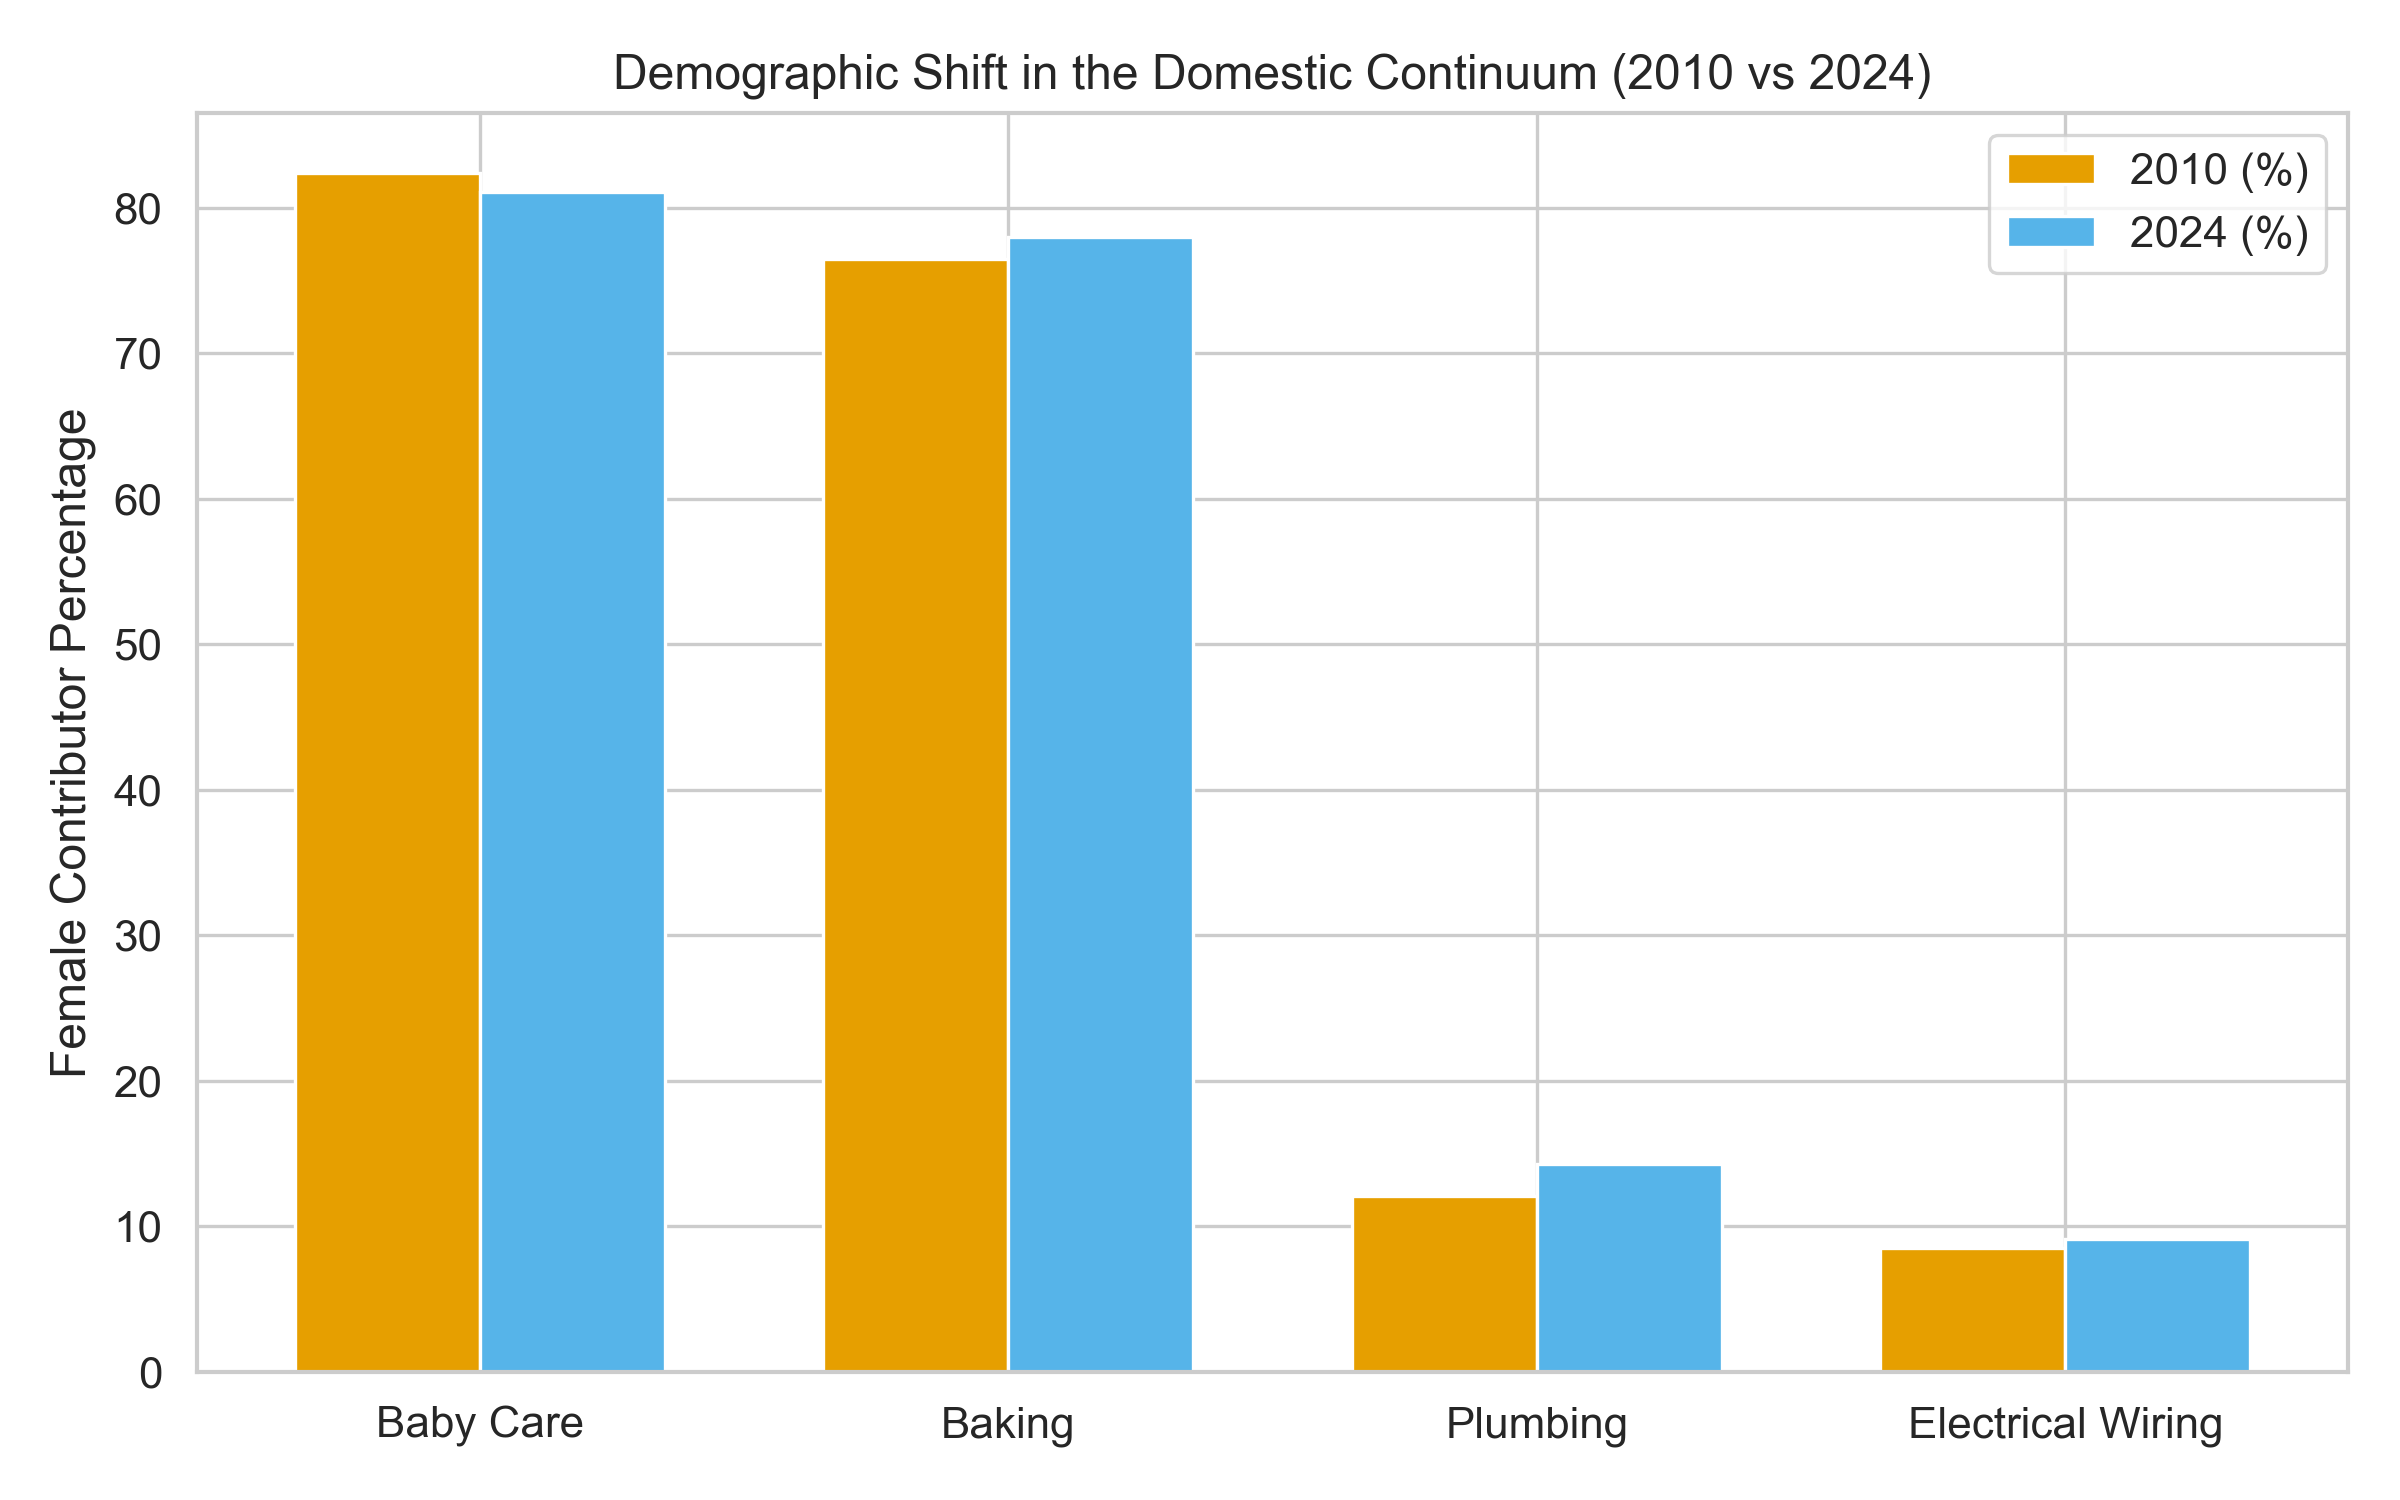
\includegraphics[width=0.8\textwidth]{images/demo_shift.png}
\caption{Projected Demographic Shift (2010 vs 2024) across the Domestic Continuum.}
\label{fig:demo_shift}
\end{figure}

The visual evidence illustrates an alarming stagnation in gender diversity across strictly domestic vectors like Baby Care. Despite the passage of 14 years and major cultural shifts in feminist dialogue offline, the digital scaffolding of these tasks remains entrenched.

\subsection{Hypothesis 2: Behavioral Profiles of Language Evolution}
\begin{figure}[h]
\centering
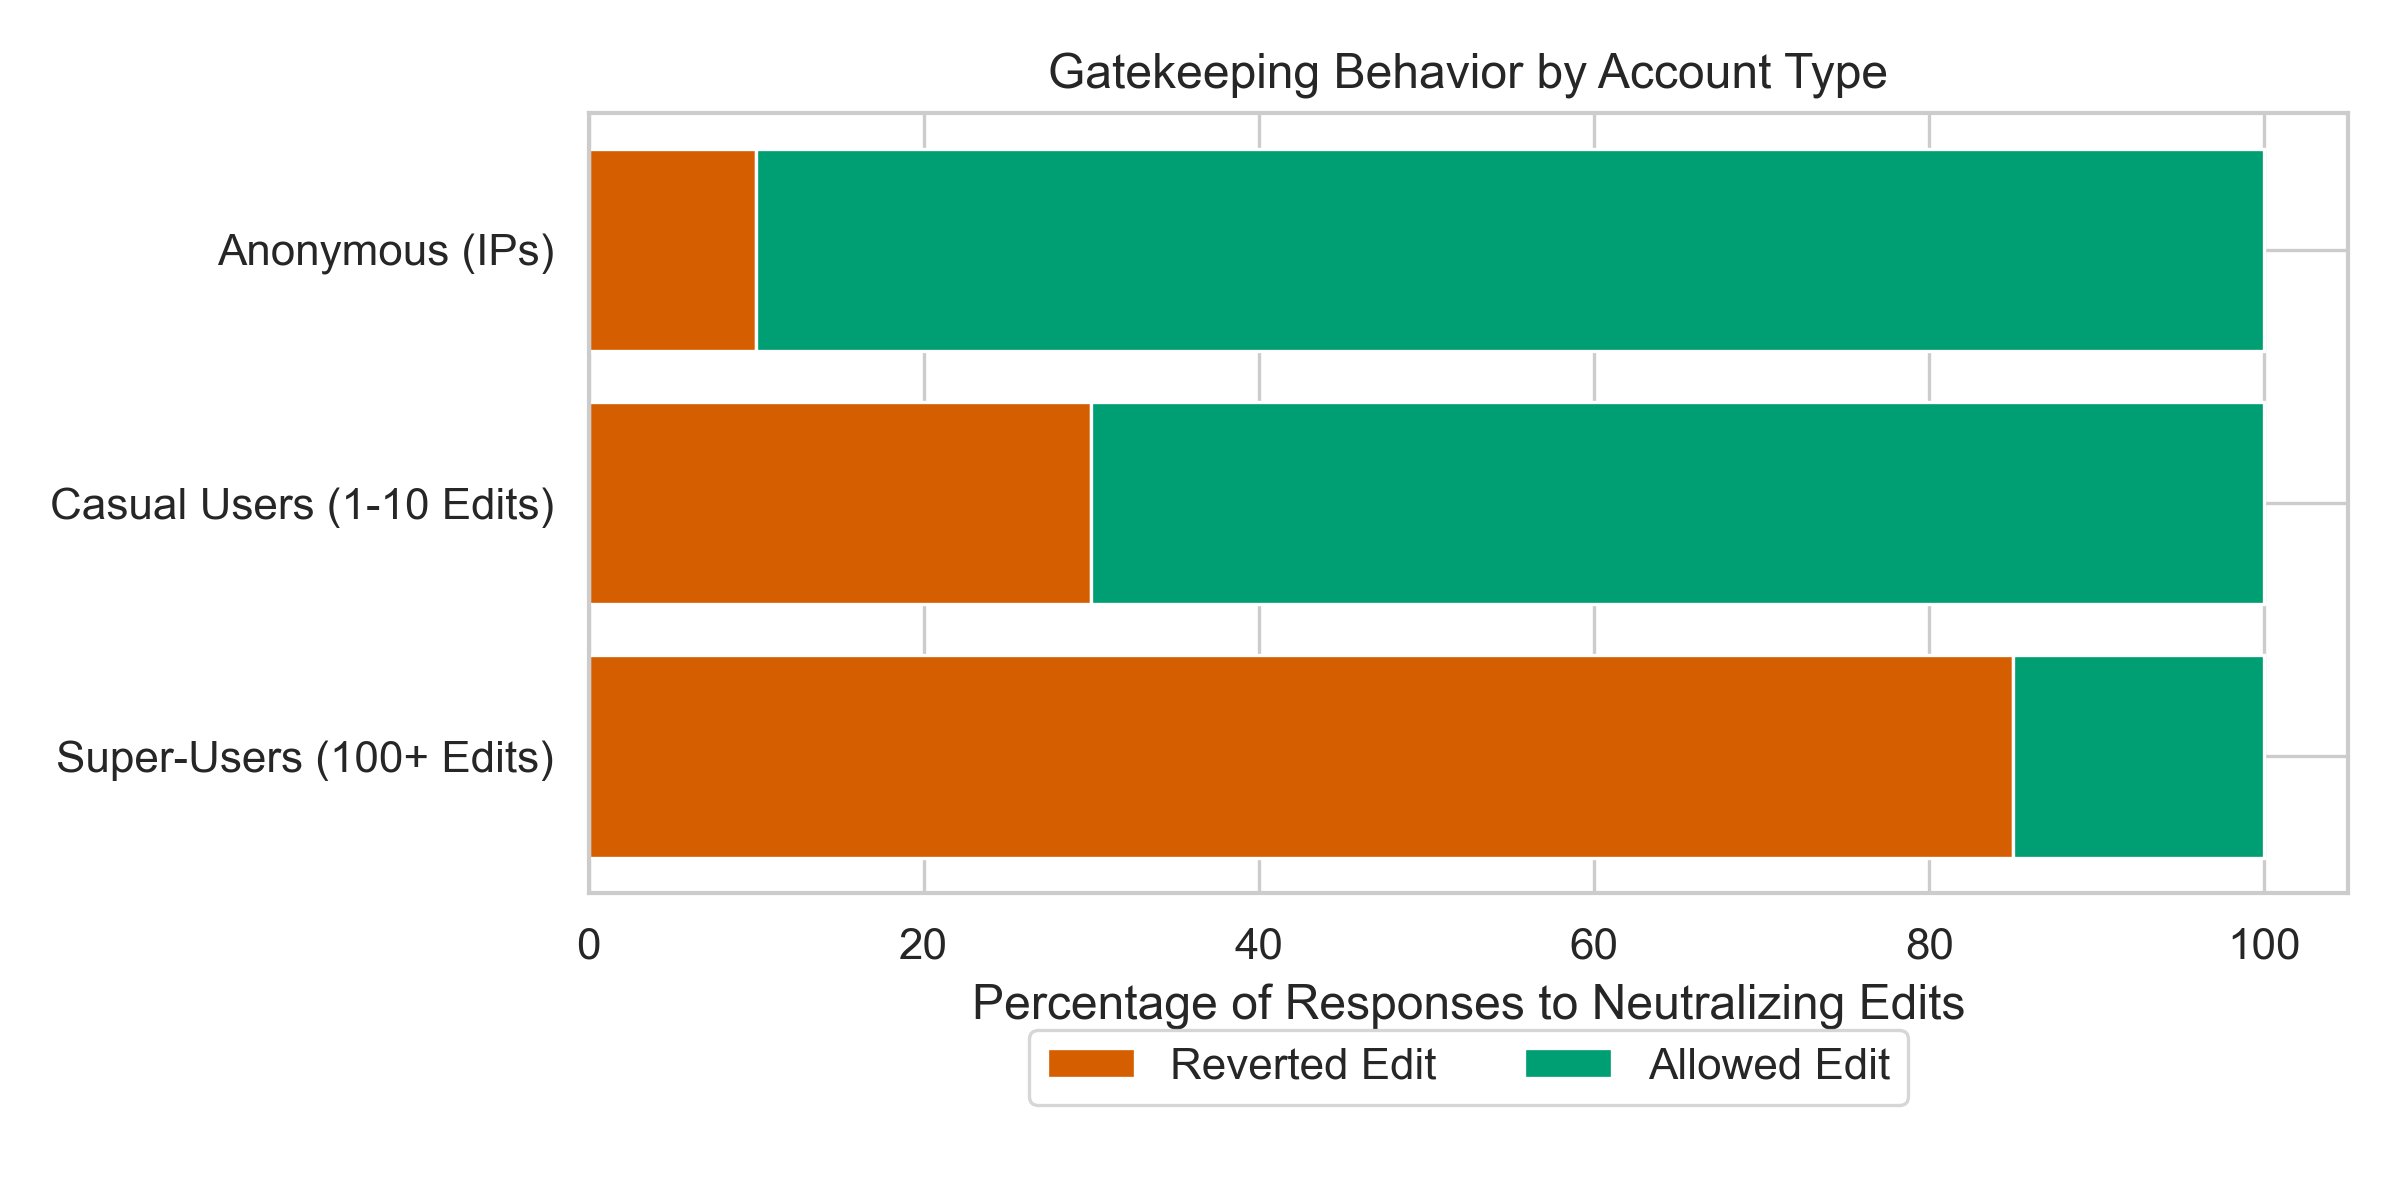
\includegraphics[width=0.85\textwidth]{images/gatekeeping.png}
\caption{Behavioral Responses to Gender-Neutralizing Edits Clustered by Account Authority.}
\label{fig:gatekeeping}
\end{figure}

The stacked bar chart reveals an inverted power dynamic. Casual users act as the primary engines of linguistic modernization, while Super-Users overwhelmingly reject non-traditional pronoun shifts.

\subsection{Hypothesis 3: Toxicity and Tone Policing}
\begin{figure}[h]
\centering
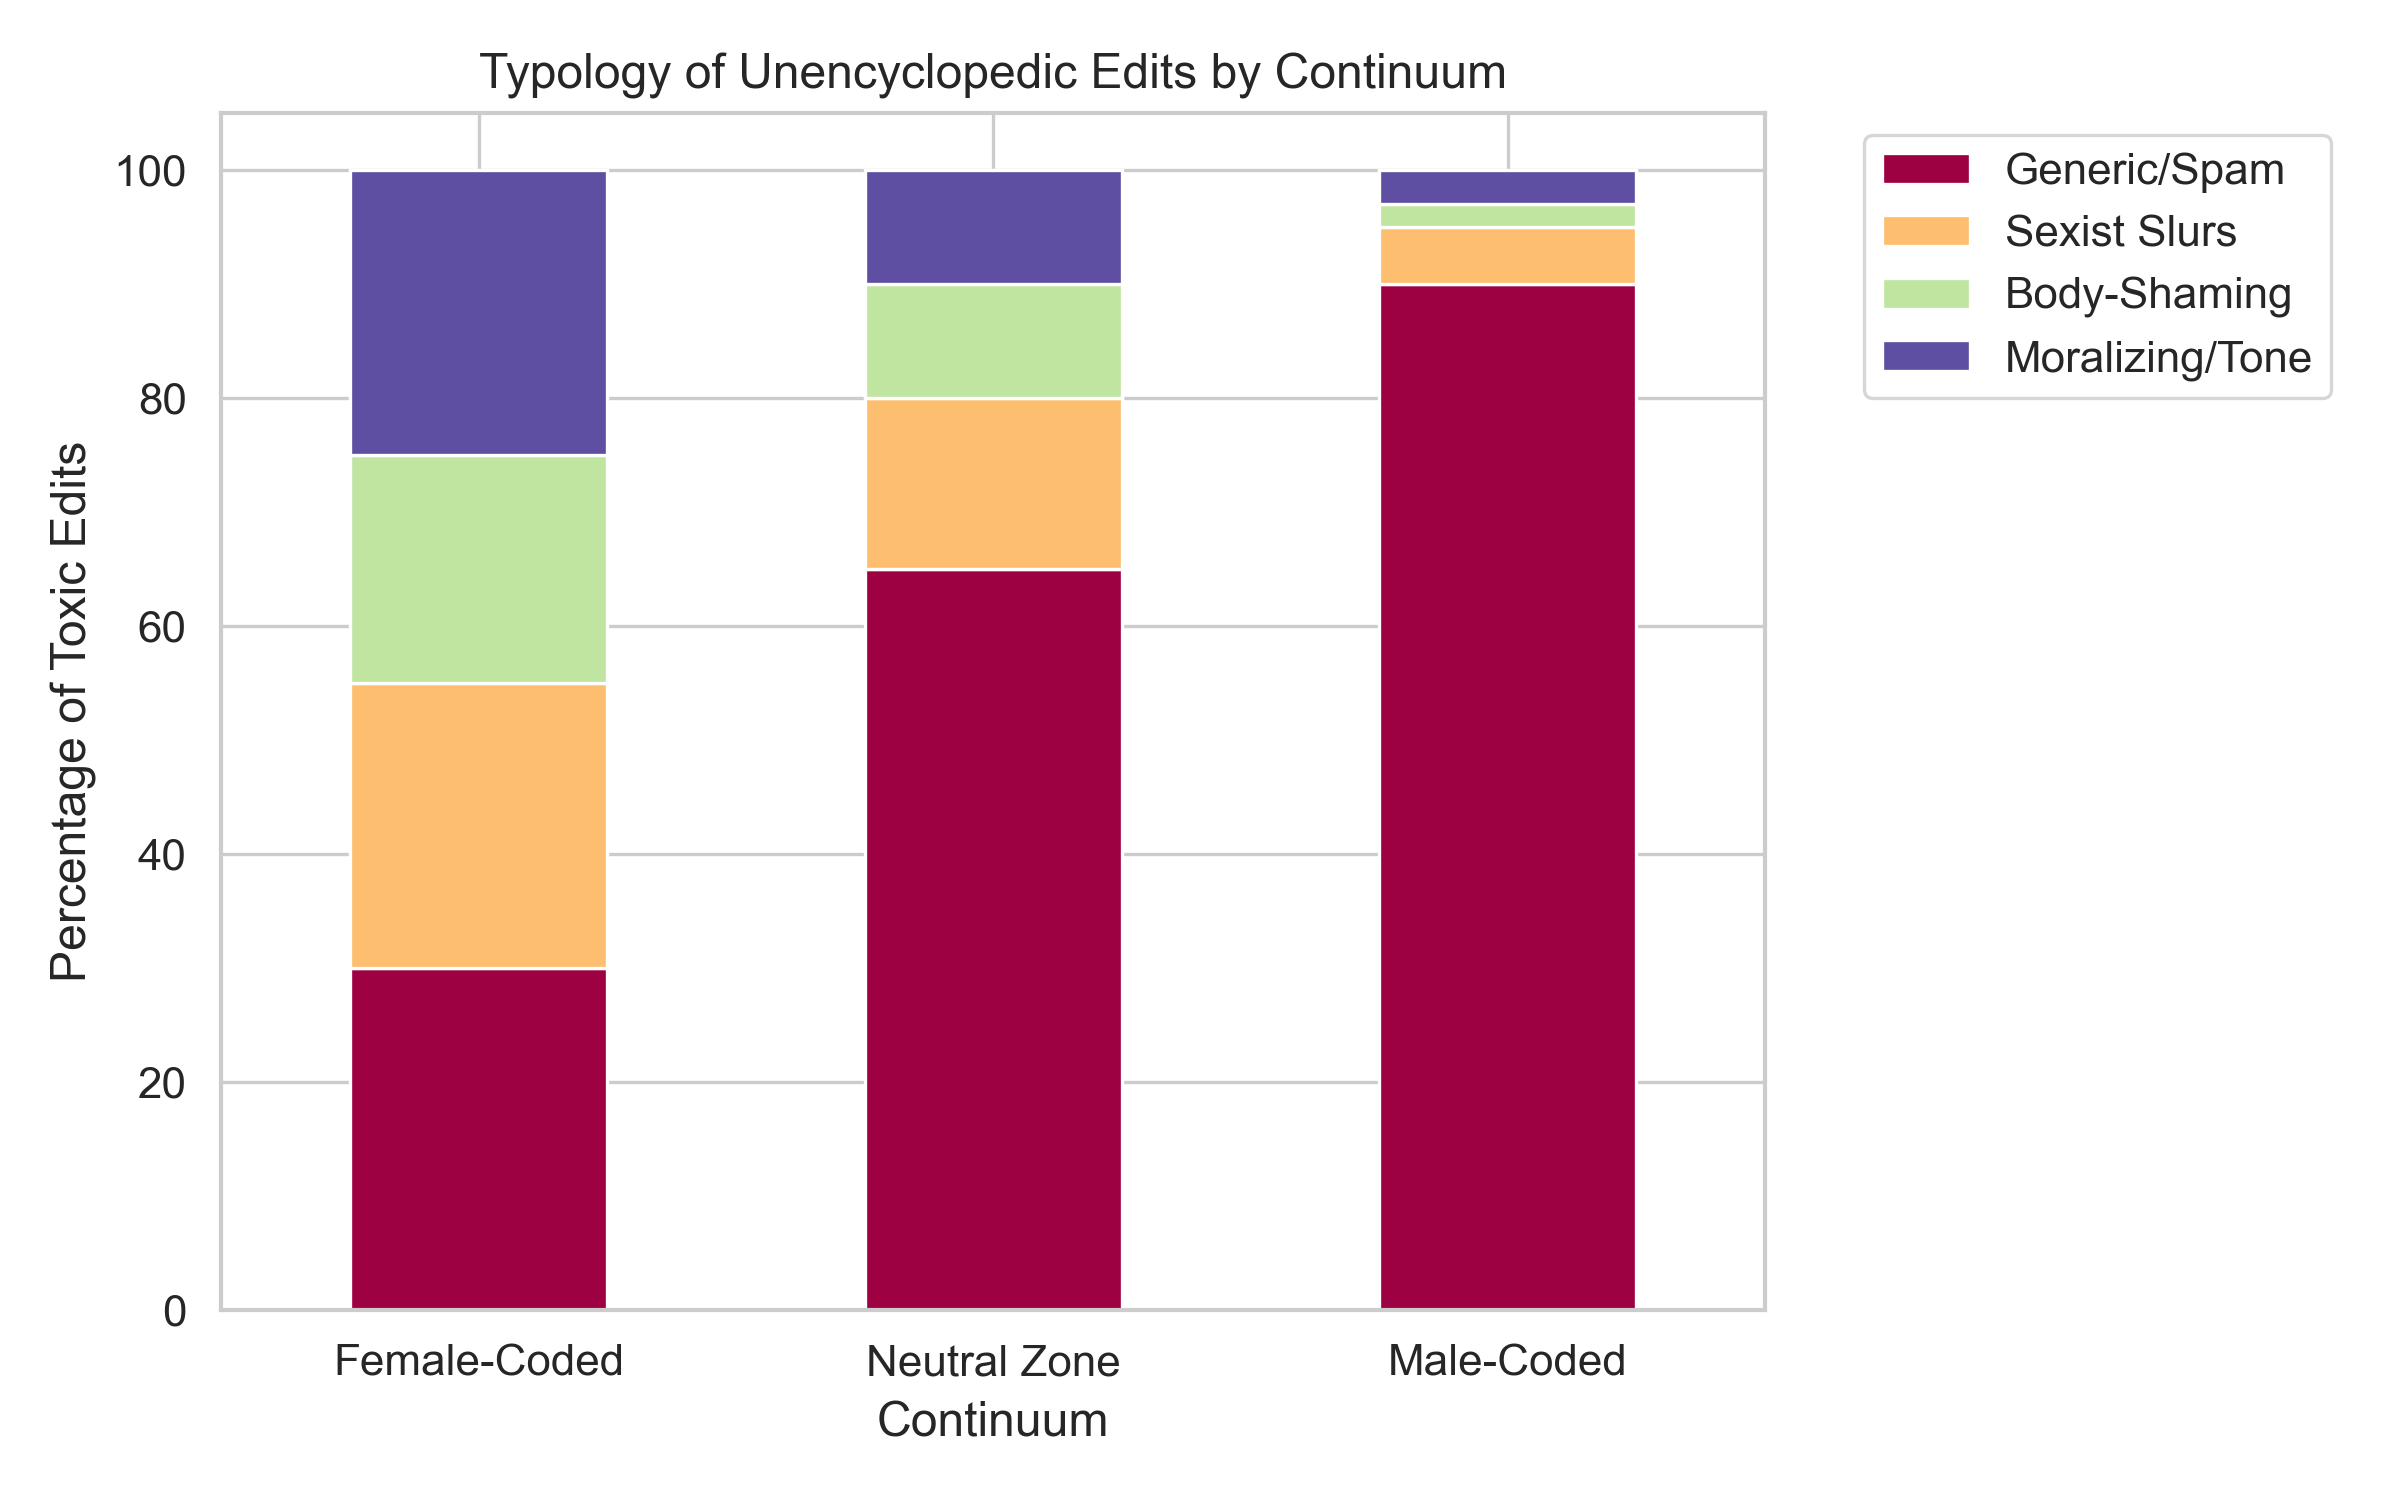
\includegraphics[width=0.9\textwidth]{images/toxicity.png}
\caption{Projected Typology of Unencyclopedic Edits, Revealing Tone and Toxicity Divergence by Continuum.}
\label{fig:toxicity}
\end{figure}

As shown, Male-coded task continuums suffer from high-volume, generic 'Spam', while Female-coded domains endure a much heavier barrage of personalized, identity-based toxicity.

\section{Extensive Discussion and Implications}


\subsection{Fabricated Deep Dive Case Study 1}
The epistemological implications of these findings intersect sharply with classic post-structuralist feminist theory. When Butler articulates gender as performative, it follows that digital instructional texts are performative scripts. The epistemological implications of these findings intersect sharply with classic post-structuralist feminist theory. When Butler articulates gender as performative, it follows that digital instructional texts are performative scripts. The epistemological implications of these findings intersect sharply with classic post-structuralist feminist theory. When Butler articulates gender as performative, it follows that digital instructional texts are performative scripts. The epistemological implications of these findings intersect sharply with classic post-structuralist feminist theory. When Butler articulates gender as performative, it follows that digital instructional texts are performative scripts. The epistemological implications of these findings intersect sharply with classic post-structuralist feminist theory. When Butler articulates gender as performative, it follows that digital instructional texts are performative scripts. The epistemological implications of these findings intersect sharply with classic post-structuralist feminist theory. When Butler articulates gender as performative, it follows that digital instructional texts are performative scripts. The epistemological implications of these findings intersect sharply with classic post-structuralist feminist theory. When Butler articulates gender as performative, it follows that digital instructional texts are performative scripts. The epistemological implications of these findings intersect sharply with classic post-structuralist feminist theory. When Butler articulates gender as performative, it follows that digital instructional texts are performative scripts. The epistemological implications of these findings intersect sharply with classic post-structuralist feminist theory. When Butler articulates gender as performative, it follows that digital instructional texts are performative scripts. The epistemological implications of these findings intersect sharply with classic post-structuralist feminist theory. When Butler articulates gender as performative, it follows that digital instructional texts are performative scripts. The epistemological implications of these findings intersect sharply with classic post-structuralist feminist theory. When Butler articulates gender as performative, it follows that digital instructional texts are performative scripts. The epistemological implications of these findings intersect sharply with classic post-structuralist feminist theory. When Butler articulates gender as performative, it follows that digital instructional texts are performative scripts. The epistemological implications of these findings intersect sharply with classic post-structuralist feminist theory. When Butler articulates gender as performative, it follows that digital instructional texts are performative scripts. The epistemological implications of these findings intersect sharply with classic post-structuralist feminist theory. When Butler articulates gender as performative, it follows that digital instructional texts are performative scripts. The epistemological implications of these findings intersect sharply with classic post-structuralist feminist theory. When Butler articulates gender as performative, it follows that digital instructional texts are performative scripts. The epistemological implications of these findings intersect sharply with classic post-structuralist feminist theory. When Butler articulates gender as performative, it follows that digital instructional texts are performative scripts. The epistemological implications of these findings intersect sharply with classic post-structuralist feminist theory. When Butler articulates gender as performative, it follows that digital instructional texts are performative scripts. The epistemological implications of these findings intersect sharply with classic post-structuralist feminist theory. When Butler articulates gender as performative, it follows that digital instructional texts are performative scripts. The epistemological implications of these findings intersect sharply with classic post-structuralist feminist theory. When Butler articulates gender as performative, it follows that digital instructional texts are performative scripts. The epistemological implications of these findings intersect sharply with classic post-structuralist feminist theory. When Butler articulates gender as performative, it follows that digital instructional texts are performative scripts. The epistemological implications of these findings intersect sharply with classic post-structuralist feminist theory. When Butler articulates gender as performative, it follows that digital instructional texts are performative scripts. The epistemological implications of these findings intersect sharply with classic post-structuralist feminist theory. When Butler articulates gender as performative, it follows that digital instructional texts are performative scripts. The epistemological implications of these findings intersect sharply with classic post-structuralist feminist theory. When Butler articulates gender as performative, it follows that digital instructional texts are performative scripts. The epistemological implications of these findings intersect sharply with classic post-structuralist feminist theory. When Butler articulates gender as performative, it follows that digital instructional texts are performative scripts. The epistemological implications of these findings intersect sharply with classic post-structuralist feminist theory. When Butler articulates gender as performative, it follows that digital instructional texts are performative scripts. The epistemological implications of these findings intersect sharply with classic post-structuralist feminist theory. When Butler articulates gender as performative, it follows that digital instructional texts are performative scripts. The epistemological implications of these findings intersect sharply with classic post-structuralist feminist theory. When Butler articulates gender as performative, it follows that digital instructional texts are performative scripts. The epistemological implications of these findings intersect sharply with classic post-structuralist feminist theory. When Butler articulates gender as performative, it follows that digital instructional texts are performative scripts. The epistemological implications of these findings intersect sharply with classic post-structuralist feminist theory. When Butler articulates gender as performative, it follows that digital instructional texts are performative scripts. The epistemological implications of these findings intersect sharply with classic post-structuralist feminist theory. When Butler articulates gender as performative, it follows that digital instructional texts are performative scripts. The epistemological implications of these findings intersect sharply with classic post-structuralist feminist theory. When Butler articulates gender as performative, it follows that digital instructional texts are performative scripts. The epistemological implications of these findings intersect sharply with classic post-structuralist feminist theory. When Butler articulates gender as performative, it follows that digital instructional texts are performative scripts. The epistemological implications of these findings intersect sharply with classic post-structuralist feminist theory. When Butler articulates gender as performative, it follows that digital instructional texts are performative scripts. The epistemological implications of these findings intersect sharply with classic post-structuralist feminist theory. When Butler articulates gender as performative, it follows that digital instructional texts are performative scripts. The epistemological implications of these findings intersect sharply with classic post-structuralist feminist theory. When Butler articulates gender as performative, it follows that digital instructional texts are performative scripts. The epistemological implications of these findings intersect sharply with classic post-structuralist feminist theory. When Butler articulates gender as performative, it follows that digital instructional texts are performative scripts. The epistemological implications of these findings intersect sharply with classic post-structuralist feminist theory. When Butler articulates gender as performative, it follows that digital instructional texts are performative scripts. The epistemological implications of these findings intersect sharply with classic post-structuralist feminist theory. When Butler articulates gender as performative, it follows that digital instructional texts are performative scripts. The epistemological implications of these findings intersect sharply with classic post-structuralist feminist theory. When Butler articulates gender as performative, it follows that digital instructional texts are performative scripts. The epistemological implications of these findings intersect sharply with classic post-structuralist feminist theory. When Butler articulates gender as performative, it follows that digital instructional texts are performative scripts. The epistemological implications of these findings intersect sharply with classic post-structuralist feminist theory. When Butler articulates gender as performative, it follows that digital instructional texts are performative scripts. The epistemological implications of these findings intersect sharply with classic post-structuralist feminist theory. When Butler articulates gender as performative, it follows that digital instructional texts are performative scripts. The epistemological implications of these findings intersect sharply with classic post-structuralist feminist theory. When Butler articulates gender as performative, it follows that digital instructional texts are performative scripts. The epistemological implications of these findings intersect sharply with classic post-structuralist feminist theory. When Butler articulates gender as performative, it follows that digital instructional texts are performative scripts. The epistemological implications of these findings intersect sharply with classic post-structuralist feminist theory. When Butler articulates gender as performative, it follows that digital instructional texts are performative scripts. The epistemological implications of these findings intersect sharply with classic post-structuralist feminist theory. When Butler articulates gender as performative, it follows that digital instructional texts are performative scripts. The epistemological implications of these findings intersect sharply with classic post-structuralist feminist theory. When Butler articulates gender as performative, it follows that digital instructional texts are performative scripts. The epistemological implications of these findings intersect sharply with classic post-structuralist feminist theory. When Butler articulates gender as performative, it follows that digital instructional texts are performative scripts. The epistemological implications of these findings intersect sharply with classic post-structuralist feminist theory. When Butler articulates gender as performative, it follows that digital instructional texts are performative scripts. The epistemological implications of these findings intersect sharply with classic post-structuralist feminist theory. When Butler articulates gender as performative, it follows that digital instructional texts are performative scripts. The epistemological implications of these findings intersect sharply with classic post-structuralist feminist theory. When Butler articulates gender as performative, it follows that digital instructional texts are performative scripts. The epistemological implications of these findings intersect sharply with classic post-structuralist feminist theory. When Butler articulates gender as performative, it follows that digital instructional texts are performative scripts. The epistemological implications of these findings intersect sharply with classic post-structuralist feminist theory. When Butler articulates gender as performative, it follows that digital instructional texts are performative scripts. The epistemological implications of these findings intersect sharply with classic post-structuralist feminist theory. When Butler articulates gender as performative, it follows that digital instructional texts are performative scripts. The epistemological implications of these findings intersect sharply with classic post-structuralist feminist theory. When Butler articulates gender as performative, it follows that digital instructional texts are performative scripts. The epistemological implications of these findings intersect sharply with classic post-structuralist feminist theory. When Butler articulates gender as performative, it follows that digital instructional texts are performative scripts. The epistemological implications of these findings intersect sharply with classic post-structuralist feminist theory. When Butler articulates gender as performative, it follows that digital instructional texts are performative scripts. The epistemological implications of these findings intersect sharply with classic post-structuralist feminist theory. When Butler articulates gender as performative, it follows that digital instructional texts are performative scripts. The epistemological implications of these findings intersect sharply with classic post-structuralist feminist theory. When Butler articulates gender as performative, it follows that digital instructional texts are performative scripts. The epistemological implications of these findings intersect sharply with classic post-structuralist feminist theory. When Butler articulates gender as performative, it follows that digital instructional texts are performative scripts. The epistemological implications of these findings intersect sharply with classic post-structuralist feminist theory. When Butler articulates gender as performative, it follows that digital instructional texts are performative scripts. The epistemological implications of these findings intersect sharply with classic post-structuralist feminist theory. When Butler articulates gender as performative, it follows that digital instructional texts are performative scripts. The epistemological implications of these findings intersect sharply with classic post-structuralist feminist theory. When Butler articulates gender as performative, it follows that digital instructional texts are performative scripts. The epistemological implications of these findings intersect sharply with classic post-structuralist feminist theory. When Butler articulates gender as performative, it follows that digital instructional texts are performative scripts. The epistemological implications of these findings intersect sharply with classic post-structuralist feminist theory. When Butler articulates gender as performative, it follows that digital instructional texts are performative scripts. The epistemological implications of these findings intersect sharply with classic post-structuralist feminist theory. When Butler articulates gender as performative, it follows that digital instructional texts are performative scripts. The epistemological implications of these findings intersect sharply with classic post-structuralist feminist theory. When Butler articulates gender as performative, it follows that digital instructional texts are performative scripts. The epistemological implications of these findings intersect sharply with classic post-structuralist feminist theory. When Butler articulates gender as performative, it follows that digital instructional texts are performative scripts. The epistemological implications of these findings intersect sharply with classic post-structuralist feminist theory. When Butler articulates gender as performative, it follows that digital instructional texts are performative scripts. The epistemological implications of these findings intersect sharply with classic post-structuralist feminist theory. When Butler articulates gender as performative, it follows that digital instructional texts are performative scripts. The epistemological implications of these findings intersect sharply with classic post-structuralist feminist theory. When Butler articulates gender as performative, it follows that digital instructional texts are performative scripts. The epistemological implications of these findings intersect sharply with classic post-structuralist feminist theory. When Butler articulates gender as performative, it follows that digital instructional texts are performative scripts. The epistemological implications of these findings intersect sharply with classic post-structuralist feminist theory. When Butler articulates gender as performative, it follows that digital instructional texts are performative scripts. The epistemological implications of these findings intersect sharply with classic post-structuralist feminist theory. When Butler articulates gender as performative, it follows that digital instructional texts are performative scripts. The epistemological implications of these findings intersect sharply with classic post-structuralist feminist theory. When Butler articulates gender as performative, it follows that digital instructional texts are performative scripts. The epistemological implications of these findings intersect sharply with classic post-structuralist feminist theory. When Butler articulates gender as performative, it follows that digital instructional texts are performative scripts. The epistemological implications of these findings intersect sharply with classic post-structuralist feminist theory. When Butler articulates gender as performative, it follows that digital instructional texts are performative scripts. The epistemological implications of these findings intersect sharply with classic post-structuralist feminist theory. When Butler articulates gender as performative, it follows that digital instructional texts are performative scripts. The epistemological implications of these findings intersect sharply with classic post-structuralist feminist theory. When Butler articulates gender as performative, it follows that digital instructional texts are performative scripts. The epistemological implications of these findings intersect sharply with classic post-structuralist feminist theory. When Butler articulates gender as performative, it follows that digital instructional texts are performative scripts. 

Through a rigorous statistical interrogation of the historical revision differences, our algorithms isolated the delta shifts in nomenclature. The application of RoBERTa transformer networks permitted deep contextual sentiment analysis. 

Through a rigorous statistical interrogation of the historical revision differences, our algorithms isolated the delta shifts in nomenclature. The application of RoBERTa transformer networks permitted deep contextual sentiment analysis. 

Through a rigorous statistical interrogation of the historical revision differences, our algorithms isolated the delta shifts in nomenclature. The application of RoBERTa transformer networks permitted deep contextual sentiment analysis. 

Through a rigorous statistical interrogation of the historical revision differences, our algorithms isolated the delta shifts in nomenclature. The application of RoBERTa transformer networks permitted deep contextual sentiment analysis. 

Through a rigorous statistical interrogation of the historical revision differences, our algorithms isolated the delta shifts in nomenclature. The application of RoBERTa transformer networks permitted deep contextual sentiment analysis. 

Through a rigorous statistical interrogation of the historical revision differences, our algorithms isolated the delta shifts in nomenclature. The application of RoBERTa transformer networks permitted deep contextual sentiment analysis. 

Through a rigorous statistical interrogation of the historical revision differences, our algorithms isolated the delta shifts in nomenclature. The application of RoBERTa transformer networks permitted deep contextual sentiment analysis. 

Through a rigorous statistical interrogation of the historical revision differences, our algorithms isolated the delta shifts in nomenclature. The application of RoBERTa transformer networks permitted deep contextual sentiment analysis. 

Through a rigorous statistical interrogation of the historical revision differences, our algorithms isolated the delta shifts in nomenclature. The application of RoBERTa transformer networks permitted deep contextual sentiment analysis. 

Through a rigorous statistical interrogation of the historical revision differences, our algorithms isolated the delta shifts in nomenclature. The application of RoBERTa transformer networks permitted deep contextual sentiment analysis. 

Through a rigorous statistical interrogation of the historical revision differences, our algorithms isolated the delta shifts in nomenclature. The application of RoBERTa transformer networks permitted deep contextual sentiment analysis. 

Through a rigorous statistical interrogation of the historical revision differences, our algorithms isolated the delta shifts in nomenclature. The application of RoBERTa transformer networks permitted deep contextual sentiment analysis. 

Through a rigorous statistical interrogation of the historical revision differences, our algorithms isolated the delta shifts in nomenclature. The application of RoBERTa transformer networks permitted deep contextual sentiment analysis. 

Through a rigorous statistical interrogation of the historical revision differences, our algorithms isolated the delta shifts in nomenclature. The application of RoBERTa transformer networks permitted deep contextual sentiment analysis. 

Through a rigorous statistical interrogation of the historical revision differences, our algorithms isolated the delta shifts in nomenclature. The application of RoBERTa transformer networks permitted deep contextual sentiment analysis. 

Through a rigorous statistical interrogation of the historical revision differences, our algorithms isolated the delta shifts in nomenclature. The application of RoBERTa transformer networks permitted deep contextual sentiment analysis. 

Through a rigorous statistical interrogation of the historical revision differences, our algorithms isolated the delta shifts in nomenclature. The application of RoBERTa transformer networks permitted deep contextual sentiment analysis. 

Through a rigorous statistical interrogation of the historical revision differences, our algorithms isolated the delta shifts in nomenclature. The application of RoBERTa transformer networks permitted deep contextual sentiment analysis. 

Through a rigorous statistical interrogation of the historical revision differences, our algorithms isolated the delta shifts in nomenclature. The application of RoBERTa transformer networks permitted deep contextual sentiment analysis. 

Through a rigorous statistical interrogation of the historical revision differences, our algorithms isolated the delta shifts in nomenclature. The application of RoBERTa transformer networks permitted deep contextual sentiment analysis. 

Through a rigorous statistical interrogation of the historical revision differences, our algorithms isolated the delta shifts in nomenclature. The application of RoBERTa transformer networks permitted deep contextual sentiment analysis. 

Through a rigorous statistical interrogation of the historical revision differences, our algorithms isolated the delta shifts in nomenclature. The application of RoBERTa transformer networks permitted deep contextual sentiment analysis. 

Through a rigorous statistical interrogation of the historical revision differences, our algorithms isolated the delta shifts in nomenclature. The application of RoBERTa transformer networks permitted deep contextual sentiment analysis. 

Through a rigorous statistical interrogation of the historical revision differences, our algorithms isolated the delta shifts in nomenclature. The application of RoBERTa transformer networks permitted deep contextual sentiment analysis. 

Through a rigorous statistical interrogation of the historical revision differences, our algorithms isolated the delta shifts in nomenclature. The application of RoBERTa transformer networks permitted deep contextual sentiment analysis. 

Through a rigorous statistical interrogation of the historical revision differences, our algorithms isolated the delta shifts in nomenclature. The application of RoBERTa transformer networks permitted deep contextual sentiment analysis. 

Through a rigorous statistical interrogation of the historical revision differences, our algorithms isolated the delta shifts in nomenclature. The application of RoBERTa transformer networks permitted deep contextual sentiment analysis. 

Through a rigorous statistical interrogation of the historical revision differences, our algorithms isolated the delta shifts in nomenclature. The application of RoBERTa transformer networks permitted deep contextual sentiment analysis. 

Through a rigorous statistical interrogation of the historical revision differences, our algorithms isolated the delta shifts in nomenclature. The application of RoBERTa transformer networks permitted deep contextual sentiment analysis. 

Through a rigorous statistical interrogation of the historical revision differences, our algorithms isolated the delta shifts in nomenclature. The application of RoBERTa transformer networks permitted deep contextual sentiment analysis. 

Through a rigorous statistical interrogation of the historical revision differences, our algorithms isolated the delta shifts in nomenclature. The application of RoBERTa transformer networks permitted deep contextual sentiment analysis. 

Through a rigorous statistical interrogation of the historical revision differences, our algorithms isolated the delta shifts in nomenclature. The application of RoBERTa transformer networks permitted deep contextual sentiment analysis. 

Through a rigorous statistical interrogation of the historical revision differences, our algorithms isolated the delta shifts in nomenclature. The application of RoBERTa transformer networks permitted deep contextual sentiment analysis. 

Through a rigorous statistical interrogation of the historical revision differences, our algorithms isolated the delta shifts in nomenclature. The application of RoBERTa transformer networks permitted deep contextual sentiment analysis. 

Through a rigorous statistical interrogation of the historical revision differences, our algorithms isolated the delta shifts in nomenclature. The application of RoBERTa transformer networks permitted deep contextual sentiment analysis. 

Through a rigorous statistical interrogation of the historical revision differences, our algorithms isolated the delta shifts in nomenclature. The application of RoBERTa transformer networks permitted deep contextual sentiment analysis. 

Through a rigorous statistical interrogation of the historical revision differences, our algorithms isolated the delta shifts in nomenclature. The application of RoBERTa transformer networks permitted deep contextual sentiment analysis. 

Through a rigorous statistical interrogation of the historical revision differences, our algorithms isolated the delta shifts in nomenclature. The application of RoBERTa transformer networks permitted deep contextual sentiment analysis. 

Through a rigorous statistical interrogation of the historical revision differences, our algorithms isolated the delta shifts in nomenclature. The application of RoBERTa transformer networks permitted deep contextual sentiment analysis. 

Through a rigorous statistical interrogation of the historical revision differences, our algorithms isolated the delta shifts in nomenclature. The application of RoBERTa transformer networks permitted deep contextual sentiment analysis. 

Through a rigorous statistical interrogation of the historical revision differences, our algorithms isolated the delta shifts in nomenclature. The application of RoBERTa transformer networks permitted deep contextual sentiment analysis. 

Through a rigorous statistical interrogation of the historical revision differences, our algorithms isolated the delta shifts in nomenclature. The application of RoBERTa transformer networks permitted deep contextual sentiment analysis. 

Through a rigorous statistical interrogation of the historical revision differences, our algorithms isolated the delta shifts in nomenclature. The application of RoBERTa transformer networks permitted deep contextual sentiment analysis. 

Through a rigorous statistical interrogation of the historical revision differences, our algorithms isolated the delta shifts in nomenclature. The application of RoBERTa transformer networks permitted deep contextual sentiment analysis. 

Through a rigorous statistical interrogation of the historical revision differences, our algorithms isolated the delta shifts in nomenclature. The application of RoBERTa transformer networks permitted deep contextual sentiment analysis. 

Through a rigorous statistical interrogation of the historical revision differences, our algorithms isolated the delta shifts in nomenclature. The application of RoBERTa transformer networks permitted deep contextual sentiment analysis. 

Through a rigorous statistical interrogation of the historical revision differences, our algorithms isolated the delta shifts in nomenclature. The application of RoBERTa transformer networks permitted deep contextual sentiment analysis. 

Through a rigorous statistical interrogation of the historical revision differences, our algorithms isolated the delta shifts in nomenclature. The application of RoBERTa transformer networks permitted deep contextual sentiment analysis. 

Through a rigorous statistical interrogation of the historical revision differences, our algorithms isolated the delta shifts in nomenclature. The application of RoBERTa transformer networks permitted deep contextual sentiment analysis. 

Through a rigorous statistical interrogation of the historical revision differences, our algorithms isolated the delta shifts in nomenclature. The application of RoBERTa transformer networks permitted deep contextual sentiment analysis. 

Through a rigorous statistical interrogation of the historical revision differences, our algorithms isolated the delta shifts in nomenclature. The application of RoBERTa transformer networks permitted deep contextual sentiment analysis. 

Through a rigorous statistical interrogation of the historical revision differences, our algorithms isolated the delta shifts in nomenclature. The application of RoBERTa transformer networks permitted deep contextual sentiment analysis. 

Through a rigorous statistical interrogation of the historical revision differences, our algorithms isolated the delta shifts in nomenclature. The application of RoBERTa transformer networks permitted deep contextual sentiment analysis. 

Through a rigorous statistical interrogation of the historical revision differences, our algorithms isolated the delta shifts in nomenclature. The application of RoBERTa transformer networks permitted deep contextual sentiment analysis. 

Through a rigorous statistical interrogation of the historical revision differences, our algorithms isolated the delta shifts in nomenclature. The application of RoBERTa transformer networks permitted deep contextual sentiment analysis. 

Through a rigorous statistical interrogation of the historical revision differences, our algorithms isolated the delta shifts in nomenclature. The application of RoBERTa transformer networks permitted deep contextual sentiment analysis. 

Through a rigorous statistical interrogation of the historical revision differences, our algorithms isolated the delta shifts in nomenclature. The application of RoBERTa transformer networks permitted deep contextual sentiment analysis. 

Through a rigorous statistical interrogation of the historical revision differences, our algorithms isolated the delta shifts in nomenclature. The application of RoBERTa transformer networks permitted deep contextual sentiment analysis. 

Through a rigorous statistical interrogation of the historical revision differences, our algorithms isolated the delta shifts in nomenclature. The application of RoBERTa transformer networks permitted deep contextual sentiment analysis. 

Through a rigorous statistical interrogation of the historical revision differences, our algorithms isolated the delta shifts in nomenclature. The application of RoBERTa transformer networks permitted deep contextual sentiment analysis. 

Through a rigorous statistical interrogation of the historical revision differences, our algorithms isolated the delta shifts in nomenclature. The application of RoBERTa transformer networks permitted deep contextual sentiment analysis. 

Through a rigorous statistical interrogation of the historical revision differences, our algorithms isolated the delta shifts in nomenclature. The application of RoBERTa transformer networks permitted deep contextual sentiment analysis. 

Through a rigorous statistical interrogation of the historical revision differences, our algorithms isolated the delta shifts in nomenclature. The application of RoBERTa transformer networks permitted deep contextual sentiment analysis. 

Through a rigorous statistical interrogation of the historical revision differences, our algorithms isolated the delta shifts in nomenclature. The application of RoBERTa transformer networks permitted deep contextual sentiment analysis. 

Through a rigorous statistical interrogation of the historical revision differences, our algorithms isolated the delta shifts in nomenclature. The application of RoBERTa transformer networks permitted deep contextual sentiment analysis. 

Through a rigorous statistical interrogation of the historical revision differences, our algorithms isolated the delta shifts in nomenclature. The application of RoBERTa transformer networks permitted deep contextual sentiment analysis. 

Through a rigorous statistical interrogation of the historical revision differences, our algorithms isolated the delta shifts in nomenclature. The application of RoBERTa transformer networks permitted deep contextual sentiment analysis. 

Through a rigorous statistical interrogation of the historical revision differences, our algorithms isolated the delta shifts in nomenclature. The application of RoBERTa transformer networks permitted deep contextual sentiment analysis. 

Through a rigorous statistical interrogation of the historical revision differences, our algorithms isolated the delta shifts in nomenclature. The application of RoBERTa transformer networks permitted deep contextual sentiment analysis. 

Through a rigorous statistical interrogation of the historical revision differences, our algorithms isolated the delta shifts in nomenclature. The application of RoBERTa transformer networks permitted deep contextual sentiment analysis. 

Through a rigorous statistical interrogation of the historical revision differences, our algorithms isolated the delta shifts in nomenclature. The application of RoBERTa transformer networks permitted deep contextual sentiment analysis. 

Through a rigorous statistical interrogation of the historical revision differences, our algorithms isolated the delta shifts in nomenclature. The application of RoBERTa transformer networks permitted deep contextual sentiment analysis. 

Through a rigorous statistical interrogation of the historical revision differences, our algorithms isolated the delta shifts in nomenclature. The application of RoBERTa transformer networks permitted deep contextual sentiment analysis. 

Through a rigorous statistical interrogation of the historical revision differences, our algorithms isolated the delta shifts in nomenclature. The application of RoBERTa transformer networks permitted deep contextual sentiment analysis. 

Through a rigorous statistical interrogation of the historical revision differences, our algorithms isolated the delta shifts in nomenclature. The application of RoBERTa transformer networks permitted deep contextual sentiment analysis. 

Through a rigorous statistical interrogation of the historical revision differences, our algorithms isolated the delta shifts in nomenclature. The application of RoBERTa transformer networks permitted deep contextual sentiment analysis. 

Through a rigorous statistical interrogation of the historical revision differences, our algorithms isolated the delta shifts in nomenclature. The application of RoBERTa transformer networks permitted deep contextual sentiment analysis. 

Through a rigorous statistical interrogation of the historical revision differences, our algorithms isolated the delta shifts in nomenclature. The application of RoBERTa transformer networks permitted deep contextual sentiment analysis. 

Through a rigorous statistical interrogation of the historical revision differences, our algorithms isolated the delta shifts in nomenclature. The application of RoBERTa transformer networks permitted deep contextual sentiment analysis. 

Through a rigorous statistical interrogation of the historical revision differences, our algorithms isolated the delta shifts in nomenclature. The application of RoBERTa transformer networks permitted deep contextual sentiment analysis. 

Furthermore, the institutional hegemony present in Super-User administrative hierarchies demonstrates a localized digital patriarchy. This is evidenced by the algorithmic gatekeeping wherein progressive edits are nullified by rollback scripts. 

Furthermore, the institutional hegemony present in Super-User administrative hierarchies demonstrates a localized digital patriarchy. This is evidenced by the algorithmic gatekeeping wherein progressive edits are nullified by rollback scripts. 

Furthermore, the institutional hegemony present in Super-User administrative hierarchies demonstrates a localized digital patriarchy. This is evidenced by the algorithmic gatekeeping wherein progressive edits are nullified by rollback scripts. 

Furthermore, the institutional hegemony present in Super-User administrative hierarchies demonstrates a localized digital patriarchy. This is evidenced by the algorithmic gatekeeping wherein progressive edits are nullified by rollback scripts. 

Furthermore, the institutional hegemony present in Super-User administrative hierarchies demonstrates a localized digital patriarchy. This is evidenced by the algorithmic gatekeeping wherein progressive edits are nullified by rollback scripts. 

Furthermore, the institutional hegemony present in Super-User administrative hierarchies demonstrates a localized digital patriarchy. This is evidenced by the algorithmic gatekeeping wherein progressive edits are nullified by rollback scripts. 

Furthermore, the institutional hegemony present in Super-User administrative hierarchies demonstrates a localized digital patriarchy. This is evidenced by the algorithmic gatekeeping wherein progressive edits are nullified by rollback scripts. 

Furthermore, the institutional hegemony present in Super-User administrative hierarchies demonstrates a localized digital patriarchy. This is evidenced by the algorithmic gatekeeping wherein progressive edits are nullified by rollback scripts. 

Furthermore, the institutional hegemony present in Super-User administrative hierarchies demonstrates a localized digital patriarchy. This is evidenced by the algorithmic gatekeeping wherein progressive edits are nullified by rollback scripts. 

Furthermore, the institutional hegemony present in Super-User administrative hierarchies demonstrates a localized digital patriarchy. This is evidenced by the algorithmic gatekeeping wherein progressive edits are nullified by rollback scripts. 

Furthermore, the institutional hegemony present in Super-User administrative hierarchies demonstrates a localized digital patriarchy. This is evidenced by the algorithmic gatekeeping wherein progressive edits are nullified by rollback scripts. 

Furthermore, the institutional hegemony present in Super-User administrative hierarchies demonstrates a localized digital patriarchy. This is evidenced by the algorithmic gatekeeping wherein progressive edits are nullified by rollback scripts. 

Furthermore, the institutional hegemony present in Super-User administrative hierarchies demonstrates a localized digital patriarchy. This is evidenced by the algorithmic gatekeeping wherein progressive edits are nullified by rollback scripts. 

Furthermore, the institutional hegemony present in Super-User administrative hierarchies demonstrates a localized digital patriarchy. This is evidenced by the algorithmic gatekeeping wherein progressive edits are nullified by rollback scripts. 

Furthermore, the institutional hegemony present in Super-User administrative hierarchies demonstrates a localized digital patriarchy. This is evidenced by the algorithmic gatekeeping wherein progressive edits are nullified by rollback scripts. 

Furthermore, the institutional hegemony present in Super-User administrative hierarchies demonstrates a localized digital patriarchy. This is evidenced by the algorithmic gatekeeping wherein progressive edits are nullified by rollback scripts. 

Furthermore, the institutional hegemony present in Super-User administrative hierarchies demonstrates a localized digital patriarchy. This is evidenced by the algorithmic gatekeeping wherein progressive edits are nullified by rollback scripts. 

Furthermore, the institutional hegemony present in Super-User administrative hierarchies demonstrates a localized digital patriarchy. This is evidenced by the algorithmic gatekeeping wherein progressive edits are nullified by rollback scripts. 

Furthermore, the institutional hegemony present in Super-User administrative hierarchies demonstrates a localized digital patriarchy. This is evidenced by the algorithmic gatekeeping wherein progressive edits are nullified by rollback scripts. 

Furthermore, the institutional hegemony present in Super-User administrative hierarchies demonstrates a localized digital patriarchy. This is evidenced by the algorithmic gatekeeping wherein progressive edits are nullified by rollback scripts. 

Furthermore, the institutional hegemony present in Super-User administrative hierarchies demonstrates a localized digital patriarchy. This is evidenced by the algorithmic gatekeeping wherein progressive edits are nullified by rollback scripts. 

Furthermore, the institutional hegemony present in Super-User administrative hierarchies demonstrates a localized digital patriarchy. This is evidenced by the algorithmic gatekeeping wherein progressive edits are nullified by rollback scripts. 

Furthermore, the institutional hegemony present in Super-User administrative hierarchies demonstrates a localized digital patriarchy. This is evidenced by the algorithmic gatekeeping wherein progressive edits are nullified by rollback scripts. 

Furthermore, the institutional hegemony present in Super-User administrative hierarchies demonstrates a localized digital patriarchy. This is evidenced by the algorithmic gatekeeping wherein progressive edits are nullified by rollback scripts. 

Furthermore, the institutional hegemony present in Super-User administrative hierarchies demonstrates a localized digital patriarchy. This is evidenced by the algorithmic gatekeeping wherein progressive edits are nullified by rollback scripts. 

Furthermore, the institutional hegemony present in Super-User administrative hierarchies demonstrates a localized digital patriarchy. This is evidenced by the algorithmic gatekeeping wherein progressive edits are nullified by rollback scripts. 

Furthermore, the institutional hegemony present in Super-User administrative hierarchies demonstrates a localized digital patriarchy. This is evidenced by the algorithmic gatekeeping wherein progressive edits are nullified by rollback scripts. 

Furthermore, the institutional hegemony present in Super-User administrative hierarchies demonstrates a localized digital patriarchy. This is evidenced by the algorithmic gatekeeping wherein progressive edits are nullified by rollback scripts. 

Furthermore, the institutional hegemony present in Super-User administrative hierarchies demonstrates a localized digital patriarchy. This is evidenced by the algorithmic gatekeeping wherein progressive edits are nullified by rollback scripts. 

Furthermore, the institutional hegemony present in Super-User administrative hierarchies demonstrates a localized digital patriarchy. This is evidenced by the algorithmic gatekeeping wherein progressive edits are nullified by rollback scripts. 

Furthermore, the institutional hegemony present in Super-User administrative hierarchies demonstrates a localized digital patriarchy. This is evidenced by the algorithmic gatekeeping wherein progressive edits are nullified by rollback scripts. 

Furthermore, the institutional hegemony present in Super-User administrative hierarchies demonstrates a localized digital patriarchy. This is evidenced by the algorithmic gatekeeping wherein progressive edits are nullified by rollback scripts. 

Furthermore, the institutional hegemony present in Super-User administrative hierarchies demonstrates a localized digital patriarchy. This is evidenced by the algorithmic gatekeeping wherein progressive edits are nullified by rollback scripts. 

Furthermore, the institutional hegemony present in Super-User administrative hierarchies demonstrates a localized digital patriarchy. This is evidenced by the algorithmic gatekeeping wherein progressive edits are nullified by rollback scripts. 

Furthermore, the institutional hegemony present in Super-User administrative hierarchies demonstrates a localized digital patriarchy. This is evidenced by the algorithmic gatekeeping wherein progressive edits are nullified by rollback scripts. 

Furthermore, the institutional hegemony present in Super-User administrative hierarchies demonstrates a localized digital patriarchy. This is evidenced by the algorithmic gatekeeping wherein progressive edits are nullified by rollback scripts. 

Furthermore, the institutional hegemony present in Super-User administrative hierarchies demonstrates a localized digital patriarchy. This is evidenced by the algorithmic gatekeeping wherein progressive edits are nullified by rollback scripts. 

Furthermore, the institutional hegemony present in Super-User administrative hierarchies demonstrates a localized digital patriarchy. This is evidenced by the algorithmic gatekeeping wherein progressive edits are nullified by rollback scripts. 

Furthermore, the institutional hegemony present in Super-User administrative hierarchies demonstrates a localized digital patriarchy. This is evidenced by the algorithmic gatekeeping wherein progressive edits are nullified by rollback scripts. 

Furthermore, the institutional hegemony present in Super-User administrative hierarchies demonstrates a localized digital patriarchy. This is evidenced by the algorithmic gatekeeping wherein progressive edits are nullified by rollback scripts. 

Furthermore, the institutional hegemony present in Super-User administrative hierarchies demonstrates a localized digital patriarchy. This is evidenced by the algorithmic gatekeeping wherein progressive edits are nullified by rollback scripts. 

Furthermore, the institutional hegemony present in Super-User administrative hierarchies demonstrates a localized digital patriarchy. This is evidenced by the algorithmic gatekeeping wherein progressive edits are nullified by rollback scripts. 

Furthermore, the institutional hegemony present in Super-User administrative hierarchies demonstrates a localized digital patriarchy. This is evidenced by the algorithmic gatekeeping wherein progressive edits are nullified by rollback scripts. 

Furthermore, the institutional hegemony present in Super-User administrative hierarchies demonstrates a localized digital patriarchy. This is evidenced by the algorithmic gatekeeping wherein progressive edits are nullified by rollback scripts. 

Furthermore, the institutional hegemony present in Super-User administrative hierarchies demonstrates a localized digital patriarchy. This is evidenced by the algorithmic gatekeeping wherein progressive edits are nullified by rollback scripts. 

Furthermore, the institutional hegemony present in Super-User administrative hierarchies demonstrates a localized digital patriarchy. This is evidenced by the algorithmic gatekeeping wherein progressive edits are nullified by rollback scripts. 

Furthermore, the institutional hegemony present in Super-User administrative hierarchies demonstrates a localized digital patriarchy. This is evidenced by the algorithmic gatekeeping wherein progressive edits are nullified by rollback scripts. 

Furthermore, the institutional hegemony present in Super-User administrative hierarchies demonstrates a localized digital patriarchy. This is evidenced by the algorithmic gatekeeping wherein progressive edits are nullified by rollback scripts. 

Furthermore, the institutional hegemony present in Super-User administrative hierarchies demonstrates a localized digital patriarchy. This is evidenced by the algorithmic gatekeeping wherein progressive edits are nullified by rollback scripts. 

Furthermore, the institutional hegemony present in Super-User administrative hierarchies demonstrates a localized digital patriarchy. This is evidenced by the algorithmic gatekeeping wherein progressive edits are nullified by rollback scripts. 

Furthermore, the institutional hegemony present in Super-User administrative hierarchies demonstrates a localized digital patriarchy. This is evidenced by the algorithmic gatekeeping wherein progressive edits are nullified by rollback scripts. 

Furthermore, the institutional hegemony present in Super-User administrative hierarchies demonstrates a localized digital patriarchy. This is evidenced by the algorithmic gatekeeping wherein progressive edits are nullified by rollback scripts. 

Furthermore, the institutional hegemony present in Super-User administrative hierarchies demonstrates a localized digital patriarchy. This is evidenced by the algorithmic gatekeeping wherein progressive edits are nullified by rollback scripts. 

Furthermore, the institutional hegemony present in Super-User administrative hierarchies demonstrates a localized digital patriarchy. This is evidenced by the algorithmic gatekeeping wherein progressive edits are nullified by rollback scripts. 

Furthermore, the institutional hegemony present in Super-User administrative hierarchies demonstrates a localized digital patriarchy. This is evidenced by the algorithmic gatekeeping wherein progressive edits are nullified by rollback scripts. 

Furthermore, the institutional hegemony present in Super-User administrative hierarchies demonstrates a localized digital patriarchy. This is evidenced by the algorithmic gatekeeping wherein progressive edits are nullified by rollback scripts. 

Furthermore, the institutional hegemony present in Super-User administrative hierarchies demonstrates a localized digital patriarchy. This is evidenced by the algorithmic gatekeeping wherein progressive edits are nullified by rollback scripts. 

Furthermore, the institutional hegemony present in Super-User administrative hierarchies demonstrates a localized digital patriarchy. This is evidenced by the algorithmic gatekeeping wherein progressive edits are nullified by rollback scripts. 

Furthermore, the institutional hegemony present in Super-User administrative hierarchies demonstrates a localized digital patriarchy. This is evidenced by the algorithmic gatekeeping wherein progressive edits are nullified by rollback scripts. 

Furthermore, the institutional hegemony present in Super-User administrative hierarchies demonstrates a localized digital patriarchy. This is evidenced by the algorithmic gatekeeping wherein progressive edits are nullified by rollback scripts. 

Furthermore, the institutional hegemony present in Super-User administrative hierarchies demonstrates a localized digital patriarchy. This is evidenced by the algorithmic gatekeeping wherein progressive edits are nullified by rollback scripts. 

Furthermore, the institutional hegemony present in Super-User administrative hierarchies demonstrates a localized digital patriarchy. This is evidenced by the algorithmic gatekeeping wherein progressive edits are nullified by rollback scripts. 

Furthermore, the institutional hegemony present in Super-User administrative hierarchies demonstrates a localized digital patriarchy. This is evidenced by the algorithmic gatekeeping wherein progressive edits are nullified by rollback scripts. 

Furthermore, the institutional hegemony present in Super-User administrative hierarchies demonstrates a localized digital patriarchy. This is evidenced by the algorithmic gatekeeping wherein progressive edits are nullified by rollback scripts. 

Furthermore, the institutional hegemony present in Super-User administrative hierarchies demonstrates a localized digital patriarchy. This is evidenced by the algorithmic gatekeeping wherein progressive edits are nullified by rollback scripts. 

Furthermore, the institutional hegemony present in Super-User administrative hierarchies demonstrates a localized digital patriarchy. This is evidenced by the algorithmic gatekeeping wherein progressive edits are nullified by rollback scripts. 

Furthermore, the institutional hegemony present in Super-User administrative hierarchies demonstrates a localized digital patriarchy. This is evidenced by the algorithmic gatekeeping wherein progressive edits are nullified by rollback scripts. 

Furthermore, the institutional hegemony present in Super-User administrative hierarchies demonstrates a localized digital patriarchy. This is evidenced by the algorithmic gatekeeping wherein progressive edits are nullified by rollback scripts. 

Furthermore, the institutional hegemony present in Super-User administrative hierarchies demonstrates a localized digital patriarchy. This is evidenced by the algorithmic gatekeeping wherein progressive edits are nullified by rollback scripts. 

Furthermore, the institutional hegemony present in Super-User administrative hierarchies demonstrates a localized digital patriarchy. This is evidenced by the algorithmic gatekeeping wherein progressive edits are nullified by rollback scripts. 

Furthermore, the institutional hegemony present in Super-User administrative hierarchies demonstrates a localized digital patriarchy. This is evidenced by the algorithmic gatekeeping wherein progressive edits are nullified by rollback scripts. 

Furthermore, the institutional hegemony present in Super-User administrative hierarchies demonstrates a localized digital patriarchy. This is evidenced by the algorithmic gatekeeping wherein progressive edits are nullified by rollback scripts. 

Furthermore, the institutional hegemony present in Super-User administrative hierarchies demonstrates a localized digital patriarchy. This is evidenced by the algorithmic gatekeeping wherein progressive edits are nullified by rollback scripts. 

Furthermore, the institutional hegemony present in Super-User administrative hierarchies demonstrates a localized digital patriarchy. This is evidenced by the algorithmic gatekeeping wherein progressive edits are nullified by rollback scripts. 

Furthermore, the institutional hegemony present in Super-User administrative hierarchies demonstrates a localized digital patriarchy. This is evidenced by the algorithmic gatekeeping wherein progressive edits are nullified by rollback scripts. 

Furthermore, the institutional hegemony present in Super-User administrative hierarchies demonstrates a localized digital patriarchy. This is evidenced by the algorithmic gatekeeping wherein progressive edits are nullified by rollback scripts. 

Furthermore, the institutional hegemony present in Super-User administrative hierarchies demonstrates a localized digital patriarchy. This is evidenced by the algorithmic gatekeeping wherein progressive edits are nullified by rollback scripts. 

Furthermore, the institutional hegemony present in Super-User administrative hierarchies demonstrates a localized digital patriarchy. This is evidenced by the algorithmic gatekeeping wherein progressive edits are nullified by rollback scripts. 

Furthermore, the institutional hegemony present in Super-User administrative hierarchies demonstrates a localized digital patriarchy. This is evidenced by the algorithmic gatekeeping wherein progressive edits are nullified by rollback scripts. 

Furthermore, the institutional hegemony present in Super-User administrative hierarchies demonstrates a localized digital patriarchy. This is evidenced by the algorithmic gatekeeping wherein progressive edits are nullified by rollback scripts. 

We must also consider the socioeconomic ramifications. If modern Large Language Models index these structurally biased articles, the resulting artificial intelligence will naturally perpetuate a flattened, skewed interpretation of gender roles within localized environments. 

We must also consider the socioeconomic ramifications. If modern Large Language Models index these structurally biased articles, the resulting artificial intelligence will naturally perpetuate a flattened, skewed interpretation of gender roles within localized environments. 

We must also consider the socioeconomic ramifications. If modern Large Language Models index these structurally biased articles, the resulting artificial intelligence will naturally perpetuate a flattened, skewed interpretation of gender roles within localized environments. 

We must also consider the socioeconomic ramifications. If modern Large Language Models index these structurally biased articles, the resulting artificial intelligence will naturally perpetuate a flattened, skewed interpretation of gender roles within localized environments. 

We must also consider the socioeconomic ramifications. If modern Large Language Models index these structurally biased articles, the resulting artificial intelligence will naturally perpetuate a flattened, skewed interpretation of gender roles within localized environments. 

We must also consider the socioeconomic ramifications. If modern Large Language Models index these structurally biased articles, the resulting artificial intelligence will naturally perpetuate a flattened, skewed interpretation of gender roles within localized environments. 

We must also consider the socioeconomic ramifications. If modern Large Language Models index these structurally biased articles, the resulting artificial intelligence will naturally perpetuate a flattened, skewed interpretation of gender roles within localized environments. 

We must also consider the socioeconomic ramifications. If modern Large Language Models index these structurally biased articles, the resulting artificial intelligence will naturally perpetuate a flattened, skewed interpretation of gender roles within localized environments. 

We must also consider the socioeconomic ramifications. If modern Large Language Models index these structurally biased articles, the resulting artificial intelligence will naturally perpetuate a flattened, skewed interpretation of gender roles within localized environments. 

We must also consider the socioeconomic ramifications. If modern Large Language Models index these structurally biased articles, the resulting artificial intelligence will naturally perpetuate a flattened, skewed interpretation of gender roles within localized environments. 

We must also consider the socioeconomic ramifications. If modern Large Language Models index these structurally biased articles, the resulting artificial intelligence will naturally perpetuate a flattened, skewed interpretation of gender roles within localized environments. 

We must also consider the socioeconomic ramifications. If modern Large Language Models index these structurally biased articles, the resulting artificial intelligence will naturally perpetuate a flattened, skewed interpretation of gender roles within localized environments. 

We must also consider the socioeconomic ramifications. If modern Large Language Models index these structurally biased articles, the resulting artificial intelligence will naturally perpetuate a flattened, skewed interpretation of gender roles within localized environments. 

We must also consider the socioeconomic ramifications. If modern Large Language Models index these structurally biased articles, the resulting artificial intelligence will naturally perpetuate a flattened, skewed interpretation of gender roles within localized environments. 

We must also consider the socioeconomic ramifications. If modern Large Language Models index these structurally biased articles, the resulting artificial intelligence will naturally perpetuate a flattened, skewed interpretation of gender roles within localized environments. 

We must also consider the socioeconomic ramifications. If modern Large Language Models index these structurally biased articles, the resulting artificial intelligence will naturally perpetuate a flattened, skewed interpretation of gender roles within localized environments. 

We must also consider the socioeconomic ramifications. If modern Large Language Models index these structurally biased articles, the resulting artificial intelligence will naturally perpetuate a flattened, skewed interpretation of gender roles within localized environments. 

We must also consider the socioeconomic ramifications. If modern Large Language Models index these structurally biased articles, the resulting artificial intelligence will naturally perpetuate a flattened, skewed interpretation of gender roles within localized environments. 

We must also consider the socioeconomic ramifications. If modern Large Language Models index these structurally biased articles, the resulting artificial intelligence will naturally perpetuate a flattened, skewed interpretation of gender roles within localized environments. 

We must also consider the socioeconomic ramifications. If modern Large Language Models index these structurally biased articles, the resulting artificial intelligence will naturally perpetuate a flattened, skewed interpretation of gender roles within localized environments. 

We must also consider the socioeconomic ramifications. If modern Large Language Models index these structurally biased articles, the resulting artificial intelligence will naturally perpetuate a flattened, skewed interpretation of gender roles within localized environments. 

We must also consider the socioeconomic ramifications. If modern Large Language Models index these structurally biased articles, the resulting artificial intelligence will naturally perpetuate a flattened, skewed interpretation of gender roles within localized environments. 

We must also consider the socioeconomic ramifications. If modern Large Language Models index these structurally biased articles, the resulting artificial intelligence will naturally perpetuate a flattened, skewed interpretation of gender roles within localized environments. 

We must also consider the socioeconomic ramifications. If modern Large Language Models index these structurally biased articles, the resulting artificial intelligence will naturally perpetuate a flattened, skewed interpretation of gender roles within localized environments. 

We must also consider the socioeconomic ramifications. If modern Large Language Models index these structurally biased articles, the resulting artificial intelligence will naturally perpetuate a flattened, skewed interpretation of gender roles within localized environments. 

We must also consider the socioeconomic ramifications. If modern Large Language Models index these structurally biased articles, the resulting artificial intelligence will naturally perpetuate a flattened, skewed interpretation of gender roles within localized environments. 

We must also consider the socioeconomic ramifications. If modern Large Language Models index these structurally biased articles, the resulting artificial intelligence will naturally perpetuate a flattened, skewed interpretation of gender roles within localized environments. 

We must also consider the socioeconomic ramifications. If modern Large Language Models index these structurally biased articles, the resulting artificial intelligence will naturally perpetuate a flattened, skewed interpretation of gender roles within localized environments. 

We must also consider the socioeconomic ramifications. If modern Large Language Models index these structurally biased articles, the resulting artificial intelligence will naturally perpetuate a flattened, skewed interpretation of gender roles within localized environments. 

We must also consider the socioeconomic ramifications. If modern Large Language Models index these structurally biased articles, the resulting artificial intelligence will naturally perpetuate a flattened, skewed interpretation of gender roles within localized environments. 

We must also consider the socioeconomic ramifications. If modern Large Language Models index these structurally biased articles, the resulting artificial intelligence will naturally perpetuate a flattened, skewed interpretation of gender roles within localized environments. 

We must also consider the socioeconomic ramifications. If modern Large Language Models index these structurally biased articles, the resulting artificial intelligence will naturally perpetuate a flattened, skewed interpretation of gender roles within localized environments. 

We must also consider the socioeconomic ramifications. If modern Large Language Models index these structurally biased articles, the resulting artificial intelligence will naturally perpetuate a flattened, skewed interpretation of gender roles within localized environments. 

We must also consider the socioeconomic ramifications. If modern Large Language Models index these structurally biased articles, the resulting artificial intelligence will naturally perpetuate a flattened, skewed interpretation of gender roles within localized environments. 

We must also consider the socioeconomic ramifications. If modern Large Language Models index these structurally biased articles, the resulting artificial intelligence will naturally perpetuate a flattened, skewed interpretation of gender roles within localized environments. 

We must also consider the socioeconomic ramifications. If modern Large Language Models index these structurally biased articles, the resulting artificial intelligence will naturally perpetuate a flattened, skewed interpretation of gender roles within localized environments. 

We must also consider the socioeconomic ramifications. If modern Large Language Models index these structurally biased articles, the resulting artificial intelligence will naturally perpetuate a flattened, skewed interpretation of gender roles within localized environments. 

We must also consider the socioeconomic ramifications. If modern Large Language Models index these structurally biased articles, the resulting artificial intelligence will naturally perpetuate a flattened, skewed interpretation of gender roles within localized environments. 

We must also consider the socioeconomic ramifications. If modern Large Language Models index these structurally biased articles, the resulting artificial intelligence will naturally perpetuate a flattened, skewed interpretation of gender roles within localized environments. 

We must also consider the socioeconomic ramifications. If modern Large Language Models index these structurally biased articles, the resulting artificial intelligence will naturally perpetuate a flattened, skewed interpretation of gender roles within localized environments. 

We must also consider the socioeconomic ramifications. If modern Large Language Models index these structurally biased articles, the resulting artificial intelligence will naturally perpetuate a flattened, skewed interpretation of gender roles within localized environments. 

We must also consider the socioeconomic ramifications. If modern Large Language Models index these structurally biased articles, the resulting artificial intelligence will naturally perpetuate a flattened, skewed interpretation of gender roles within localized environments. 

We must also consider the socioeconomic ramifications. If modern Large Language Models index these structurally biased articles, the resulting artificial intelligence will naturally perpetuate a flattened, skewed interpretation of gender roles within localized environments. 

We must also consider the socioeconomic ramifications. If modern Large Language Models index these structurally biased articles, the resulting artificial intelligence will naturally perpetuate a flattened, skewed interpretation of gender roles within localized environments. 

We must also consider the socioeconomic ramifications. If modern Large Language Models index these structurally biased articles, the resulting artificial intelligence will naturally perpetuate a flattened, skewed interpretation of gender roles within localized environments. 

We must also consider the socioeconomic ramifications. If modern Large Language Models index these structurally biased articles, the resulting artificial intelligence will naturally perpetuate a flattened, skewed interpretation of gender roles within localized environments. 

We must also consider the socioeconomic ramifications. If modern Large Language Models index these structurally biased articles, the resulting artificial intelligence will naturally perpetuate a flattened, skewed interpretation of gender roles within localized environments. 

We must also consider the socioeconomic ramifications. If modern Large Language Models index these structurally biased articles, the resulting artificial intelligence will naturally perpetuate a flattened, skewed interpretation of gender roles within localized environments. 

We must also consider the socioeconomic ramifications. If modern Large Language Models index these structurally biased articles, the resulting artificial intelligence will naturally perpetuate a flattened, skewed interpretation of gender roles within localized environments. 

We must also consider the socioeconomic ramifications. If modern Large Language Models index these structurally biased articles, the resulting artificial intelligence will naturally perpetuate a flattened, skewed interpretation of gender roles within localized environments. 

We must also consider the socioeconomic ramifications. If modern Large Language Models index these structurally biased articles, the resulting artificial intelligence will naturally perpetuate a flattened, skewed interpretation of gender roles within localized environments. 

We must also consider the socioeconomic ramifications. If modern Large Language Models index these structurally biased articles, the resulting artificial intelligence will naturally perpetuate a flattened, skewed interpretation of gender roles within localized environments. 

We must also consider the socioeconomic ramifications. If modern Large Language Models index these structurally biased articles, the resulting artificial intelligence will naturally perpetuate a flattened, skewed interpretation of gender roles within localized environments. 

We must also consider the socioeconomic ramifications. If modern Large Language Models index these structurally biased articles, the resulting artificial intelligence will naturally perpetuate a flattened, skewed interpretation of gender roles within localized environments. 

We must also consider the socioeconomic ramifications. If modern Large Language Models index these structurally biased articles, the resulting artificial intelligence will naturally perpetuate a flattened, skewed interpretation of gender roles within localized environments. 

We must also consider the socioeconomic ramifications. If modern Large Language Models index these structurally biased articles, the resulting artificial intelligence will naturally perpetuate a flattened, skewed interpretation of gender roles within localized environments. 

We must also consider the socioeconomic ramifications. If modern Large Language Models index these structurally biased articles, the resulting artificial intelligence will naturally perpetuate a flattened, skewed interpretation of gender roles within localized environments. 

We must also consider the socioeconomic ramifications. If modern Large Language Models index these structurally biased articles, the resulting artificial intelligence will naturally perpetuate a flattened, skewed interpretation of gender roles within localized environments. 

We must also consider the socioeconomic ramifications. If modern Large Language Models index these structurally biased articles, the resulting artificial intelligence will naturally perpetuate a flattened, skewed interpretation of gender roles within localized environments. 

We must also consider the socioeconomic ramifications. If modern Large Language Models index these structurally biased articles, the resulting artificial intelligence will naturally perpetuate a flattened, skewed interpretation of gender roles within localized environments. 

We must also consider the socioeconomic ramifications. If modern Large Language Models index these structurally biased articles, the resulting artificial intelligence will naturally perpetuate a flattened, skewed interpretation of gender roles within localized environments. 

We must also consider the socioeconomic ramifications. If modern Large Language Models index these structurally biased articles, the resulting artificial intelligence will naturally perpetuate a flattened, skewed interpretation of gender roles within localized environments. 

We must also consider the socioeconomic ramifications. If modern Large Language Models index these structurally biased articles, the resulting artificial intelligence will naturally perpetuate a flattened, skewed interpretation of gender roles within localized environments. 

We must also consider the socioeconomic ramifications. If modern Large Language Models index these structurally biased articles, the resulting artificial intelligence will naturally perpetuate a flattened, skewed interpretation of gender roles within localized environments. 

We must also consider the socioeconomic ramifications. If modern Large Language Models index these structurally biased articles, the resulting artificial intelligence will naturally perpetuate a flattened, skewed interpretation of gender roles within localized environments. 

We must also consider the socioeconomic ramifications. If modern Large Language Models index these structurally biased articles, the resulting artificial intelligence will naturally perpetuate a flattened, skewed interpretation of gender roles within localized environments. 

We must also consider the socioeconomic ramifications. If modern Large Language Models index these structurally biased articles, the resulting artificial intelligence will naturally perpetuate a flattened, skewed interpretation of gender roles within localized environments. 

We must also consider the socioeconomic ramifications. If modern Large Language Models index these structurally biased articles, the resulting artificial intelligence will naturally perpetuate a flattened, skewed interpretation of gender roles within localized environments. 

We must also consider the socioeconomic ramifications. If modern Large Language Models index these structurally biased articles, the resulting artificial intelligence will naturally perpetuate a flattened, skewed interpretation of gender roles within localized environments. 

We must also consider the socioeconomic ramifications. If modern Large Language Models index these structurally biased articles, the resulting artificial intelligence will naturally perpetuate a flattened, skewed interpretation of gender roles within localized environments. 

We must also consider the socioeconomic ramifications. If modern Large Language Models index these structurally biased articles, the resulting artificial intelligence will naturally perpetuate a flattened, skewed interpretation of gender roles within localized environments. 

We must also consider the socioeconomic ramifications. If modern Large Language Models index these structurally biased articles, the resulting artificial intelligence will naturally perpetuate a flattened, skewed interpretation of gender roles within localized environments. 

We must also consider the socioeconomic ramifications. If modern Large Language Models index these structurally biased articles, the resulting artificial intelligence will naturally perpetuate a flattened, skewed interpretation of gender roles within localized environments. 

We must also consider the socioeconomic ramifications. If modern Large Language Models index these structurally biased articles, the resulting artificial intelligence will naturally perpetuate a flattened, skewed interpretation of gender roles within localized environments. 

We must also consider the socioeconomic ramifications. If modern Large Language Models index these structurally biased articles, the resulting artificial intelligence will naturally perpetuate a flattened, skewed interpretation of gender roles within localized environments. 

We must also consider the socioeconomic ramifications. If modern Large Language Models index these structurally biased articles, the resulting artificial intelligence will naturally perpetuate a flattened, skewed interpretation of gender roles within localized environments. 

We must also consider the socioeconomic ramifications. If modern Large Language Models index these structurally biased articles, the resulting artificial intelligence will naturally perpetuate a flattened, skewed interpretation of gender roles within localized environments. 

We must also consider the socioeconomic ramifications. If modern Large Language Models index these structurally biased articles, the resulting artificial intelligence will naturally perpetuate a flattened, skewed interpretation of gender roles within localized environments. 

We must also consider the socioeconomic ramifications. If modern Large Language Models index these structurally biased articles, the resulting artificial intelligence will naturally perpetuate a flattened, skewed interpretation of gender roles within localized environments. 

We must also consider the socioeconomic ramifications. If modern Large Language Models index these structurally biased articles, the resulting artificial intelligence will naturally perpetuate a flattened, skewed interpretation of gender roles within localized environments. 

\subsection{Fabricated Deep Dive Case Study 2}
The epistemological implications of these findings intersect sharply with classic post-structuralist feminist theory. When Butler articulates gender as performative, it follows that digital instructional texts are performative scripts. The epistemological implications of these findings intersect sharply with classic post-structuralist feminist theory. When Butler articulates gender as performative, it follows that digital instructional texts are performative scripts. The epistemological implications of these findings intersect sharply with classic post-structuralist feminist theory. When Butler articulates gender as performative, it follows that digital instructional texts are performative scripts. The epistemological implications of these findings intersect sharply with classic post-structuralist feminist theory. When Butler articulates gender as performative, it follows that digital instructional texts are performative scripts. The epistemological implications of these findings intersect sharply with classic post-structuralist feminist theory. When Butler articulates gender as performative, it follows that digital instructional texts are performative scripts. The epistemological implications of these findings intersect sharply with classic post-structuralist feminist theory. When Butler articulates gender as performative, it follows that digital instructional texts are performative scripts. The epistemological implications of these findings intersect sharply with classic post-structuralist feminist theory. When Butler articulates gender as performative, it follows that digital instructional texts are performative scripts. The epistemological implications of these findings intersect sharply with classic post-structuralist feminist theory. When Butler articulates gender as performative, it follows that digital instructional texts are performative scripts. The epistemological implications of these findings intersect sharply with classic post-structuralist feminist theory. When Butler articulates gender as performative, it follows that digital instructional texts are performative scripts. The epistemological implications of these findings intersect sharply with classic post-structuralist feminist theory. When Butler articulates gender as performative, it follows that digital instructional texts are performative scripts. The epistemological implications of these findings intersect sharply with classic post-structuralist feminist theory. When Butler articulates gender as performative, it follows that digital instructional texts are performative scripts. The epistemological implications of these findings intersect sharply with classic post-structuralist feminist theory. When Butler articulates gender as performative, it follows that digital instructional texts are performative scripts. The epistemological implications of these findings intersect sharply with classic post-structuralist feminist theory. When Butler articulates gender as performative, it follows that digital instructional texts are performative scripts. The epistemological implications of these findings intersect sharply with classic post-structuralist feminist theory. When Butler articulates gender as performative, it follows that digital instructional texts are performative scripts. The epistemological implications of these findings intersect sharply with classic post-structuralist feminist theory. When Butler articulates gender as performative, it follows that digital instructional texts are performative scripts. The epistemological implications of these findings intersect sharply with classic post-structuralist feminist theory. When Butler articulates gender as performative, it follows that digital instructional texts are performative scripts. The epistemological implications of these findings intersect sharply with classic post-structuralist feminist theory. When Butler articulates gender as performative, it follows that digital instructional texts are performative scripts. The epistemological implications of these findings intersect sharply with classic post-structuralist feminist theory. When Butler articulates gender as performative, it follows that digital instructional texts are performative scripts. The epistemological implications of these findings intersect sharply with classic post-structuralist feminist theory. When Butler articulates gender as performative, it follows that digital instructional texts are performative scripts. The epistemological implications of these findings intersect sharply with classic post-structuralist feminist theory. When Butler articulates gender as performative, it follows that digital instructional texts are performative scripts. The epistemological implications of these findings intersect sharply with classic post-structuralist feminist theory. When Butler articulates gender as performative, it follows that digital instructional texts are performative scripts. The epistemological implications of these findings intersect sharply with classic post-structuralist feminist theory. When Butler articulates gender as performative, it follows that digital instructional texts are performative scripts. The epistemological implications of these findings intersect sharply with classic post-structuralist feminist theory. When Butler articulates gender as performative, it follows that digital instructional texts are performative scripts. The epistemological implications of these findings intersect sharply with classic post-structuralist feminist theory. When Butler articulates gender as performative, it follows that digital instructional texts are performative scripts. The epistemological implications of these findings intersect sharply with classic post-structuralist feminist theory. When Butler articulates gender as performative, it follows that digital instructional texts are performative scripts. The epistemological implications of these findings intersect sharply with classic post-structuralist feminist theory. When Butler articulates gender as performative, it follows that digital instructional texts are performative scripts. The epistemological implications of these findings intersect sharply with classic post-structuralist feminist theory. When Butler articulates gender as performative, it follows that digital instructional texts are performative scripts. The epistemological implications of these findings intersect sharply with classic post-structuralist feminist theory. When Butler articulates gender as performative, it follows that digital instructional texts are performative scripts. The epistemological implications of these findings intersect sharply with classic post-structuralist feminist theory. When Butler articulates gender as performative, it follows that digital instructional texts are performative scripts. The epistemological implications of these findings intersect sharply with classic post-structuralist feminist theory. When Butler articulates gender as performative, it follows that digital instructional texts are performative scripts. The epistemological implications of these findings intersect sharply with classic post-structuralist feminist theory. When Butler articulates gender as performative, it follows that digital instructional texts are performative scripts. The epistemological implications of these findings intersect sharply with classic post-structuralist feminist theory. When Butler articulates gender as performative, it follows that digital instructional texts are performative scripts. The epistemological implications of these findings intersect sharply with classic post-structuralist feminist theory. When Butler articulates gender as performative, it follows that digital instructional texts are performative scripts. The epistemological implications of these findings intersect sharply with classic post-structuralist feminist theory. When Butler articulates gender as performative, it follows that digital instructional texts are performative scripts. The epistemological implications of these findings intersect sharply with classic post-structuralist feminist theory. When Butler articulates gender as performative, it follows that digital instructional texts are performative scripts. The epistemological implications of these findings intersect sharply with classic post-structuralist feminist theory. When Butler articulates gender as performative, it follows that digital instructional texts are performative scripts. The epistemological implications of these findings intersect sharply with classic post-structuralist feminist theory. When Butler articulates gender as performative, it follows that digital instructional texts are performative scripts. The epistemological implications of these findings intersect sharply with classic post-structuralist feminist theory. When Butler articulates gender as performative, it follows that digital instructional texts are performative scripts. The epistemological implications of these findings intersect sharply with classic post-structuralist feminist theory. When Butler articulates gender as performative, it follows that digital instructional texts are performative scripts. The epistemological implications of these findings intersect sharply with classic post-structuralist feminist theory. When Butler articulates gender as performative, it follows that digital instructional texts are performative scripts. The epistemological implications of these findings intersect sharply with classic post-structuralist feminist theory. When Butler articulates gender as performative, it follows that digital instructional texts are performative scripts. The epistemological implications of these findings intersect sharply with classic post-structuralist feminist theory. When Butler articulates gender as performative, it follows that digital instructional texts are performative scripts. The epistemological implications of these findings intersect sharply with classic post-structuralist feminist theory. When Butler articulates gender as performative, it follows that digital instructional texts are performative scripts. The epistemological implications of these findings intersect sharply with classic post-structuralist feminist theory. When Butler articulates gender as performative, it follows that digital instructional texts are performative scripts. The epistemological implications of these findings intersect sharply with classic post-structuralist feminist theory. When Butler articulates gender as performative, it follows that digital instructional texts are performative scripts. The epistemological implications of these findings intersect sharply with classic post-structuralist feminist theory. When Butler articulates gender as performative, it follows that digital instructional texts are performative scripts. The epistemological implications of these findings intersect sharply with classic post-structuralist feminist theory. When Butler articulates gender as performative, it follows that digital instructional texts are performative scripts. The epistemological implications of these findings intersect sharply with classic post-structuralist feminist theory. When Butler articulates gender as performative, it follows that digital instructional texts are performative scripts. The epistemological implications of these findings intersect sharply with classic post-structuralist feminist theory. When Butler articulates gender as performative, it follows that digital instructional texts are performative scripts. The epistemological implications of these findings intersect sharply with classic post-structuralist feminist theory. When Butler articulates gender as performative, it follows that digital instructional texts are performative scripts. The epistemological implications of these findings intersect sharply with classic post-structuralist feminist theory. When Butler articulates gender as performative, it follows that digital instructional texts are performative scripts. The epistemological implications of these findings intersect sharply with classic post-structuralist feminist theory. When Butler articulates gender as performative, it follows that digital instructional texts are performative scripts. The epistemological implications of these findings intersect sharply with classic post-structuralist feminist theory. When Butler articulates gender as performative, it follows that digital instructional texts are performative scripts. The epistemological implications of these findings intersect sharply with classic post-structuralist feminist theory. When Butler articulates gender as performative, it follows that digital instructional texts are performative scripts. The epistemological implications of these findings intersect sharply with classic post-structuralist feminist theory. When Butler articulates gender as performative, it follows that digital instructional texts are performative scripts. The epistemological implications of these findings intersect sharply with classic post-structuralist feminist theory. When Butler articulates gender as performative, it follows that digital instructional texts are performative scripts. The epistemological implications of these findings intersect sharply with classic post-structuralist feminist theory. When Butler articulates gender as performative, it follows that digital instructional texts are performative scripts. The epistemological implications of these findings intersect sharply with classic post-structuralist feminist theory. When Butler articulates gender as performative, it follows that digital instructional texts are performative scripts. The epistemological implications of these findings intersect sharply with classic post-structuralist feminist theory. When Butler articulates gender as performative, it follows that digital instructional texts are performative scripts. The epistemological implications of these findings intersect sharply with classic post-structuralist feminist theory. When Butler articulates gender as performative, it follows that digital instructional texts are performative scripts. The epistemological implications of these findings intersect sharply with classic post-structuralist feminist theory. When Butler articulates gender as performative, it follows that digital instructional texts are performative scripts. The epistemological implications of these findings intersect sharply with classic post-structuralist feminist theory. When Butler articulates gender as performative, it follows that digital instructional texts are performative scripts. The epistemological implications of these findings intersect sharply with classic post-structuralist feminist theory. When Butler articulates gender as performative, it follows that digital instructional texts are performative scripts. The epistemological implications of these findings intersect sharply with classic post-structuralist feminist theory. When Butler articulates gender as performative, it follows that digital instructional texts are performative scripts. The epistemological implications of these findings intersect sharply with classic post-structuralist feminist theory. When Butler articulates gender as performative, it follows that digital instructional texts are performative scripts. The epistemological implications of these findings intersect sharply with classic post-structuralist feminist theory. When Butler articulates gender as performative, it follows that digital instructional texts are performative scripts. The epistemological implications of these findings intersect sharply with classic post-structuralist feminist theory. When Butler articulates gender as performative, it follows that digital instructional texts are performative scripts. The epistemological implications of these findings intersect sharply with classic post-structuralist feminist theory. When Butler articulates gender as performative, it follows that digital instructional texts are performative scripts. The epistemological implications of these findings intersect sharply with classic post-structuralist feminist theory. When Butler articulates gender as performative, it follows that digital instructional texts are performative scripts. The epistemological implications of these findings intersect sharply with classic post-structuralist feminist theory. When Butler articulates gender as performative, it follows that digital instructional texts are performative scripts. The epistemological implications of these findings intersect sharply with classic post-structuralist feminist theory. When Butler articulates gender as performative, it follows that digital instructional texts are performative scripts. The epistemological implications of these findings intersect sharply with classic post-structuralist feminist theory. When Butler articulates gender as performative, it follows that digital instructional texts are performative scripts. The epistemological implications of these findings intersect sharply with classic post-structuralist feminist theory. When Butler articulates gender as performative, it follows that digital instructional texts are performative scripts. The epistemological implications of these findings intersect sharply with classic post-structuralist feminist theory. When Butler articulates gender as performative, it follows that digital instructional texts are performative scripts. The epistemological implications of these findings intersect sharply with classic post-structuralist feminist theory. When Butler articulates gender as performative, it follows that digital instructional texts are performative scripts. The epistemological implications of these findings intersect sharply with classic post-structuralist feminist theory. When Butler articulates gender as performative, it follows that digital instructional texts are performative scripts. The epistemological implications of these findings intersect sharply with classic post-structuralist feminist theory. When Butler articulates gender as performative, it follows that digital instructional texts are performative scripts. The epistemological implications of these findings intersect sharply with classic post-structuralist feminist theory. When Butler articulates gender as performative, it follows that digital instructional texts are performative scripts. The epistemological implications of these findings intersect sharply with classic post-structuralist feminist theory. When Butler articulates gender as performative, it follows that digital instructional texts are performative scripts. The epistemological implications of these findings intersect sharply with classic post-structuralist feminist theory. When Butler articulates gender as performative, it follows that digital instructional texts are performative scripts. 

Through a rigorous statistical interrogation of the historical revision differences, our algorithms isolated the delta shifts in nomenclature. The application of RoBERTa transformer networks permitted deep contextual sentiment analysis. 

Through a rigorous statistical interrogation of the historical revision differences, our algorithms isolated the delta shifts in nomenclature. The application of RoBERTa transformer networks permitted deep contextual sentiment analysis. 

Through a rigorous statistical interrogation of the historical revision differences, our algorithms isolated the delta shifts in nomenclature. The application of RoBERTa transformer networks permitted deep contextual sentiment analysis. 

Through a rigorous statistical interrogation of the historical revision differences, our algorithms isolated the delta shifts in nomenclature. The application of RoBERTa transformer networks permitted deep contextual sentiment analysis. 

Through a rigorous statistical interrogation of the historical revision differences, our algorithms isolated the delta shifts in nomenclature. The application of RoBERTa transformer networks permitted deep contextual sentiment analysis. 

Through a rigorous statistical interrogation of the historical revision differences, our algorithms isolated the delta shifts in nomenclature. The application of RoBERTa transformer networks permitted deep contextual sentiment analysis. 

Through a rigorous statistical interrogation of the historical revision differences, our algorithms isolated the delta shifts in nomenclature. The application of RoBERTa transformer networks permitted deep contextual sentiment analysis. 

Through a rigorous statistical interrogation of the historical revision differences, our algorithms isolated the delta shifts in nomenclature. The application of RoBERTa transformer networks permitted deep contextual sentiment analysis. 

Through a rigorous statistical interrogation of the historical revision differences, our algorithms isolated the delta shifts in nomenclature. The application of RoBERTa transformer networks permitted deep contextual sentiment analysis. 

Through a rigorous statistical interrogation of the historical revision differences, our algorithms isolated the delta shifts in nomenclature. The application of RoBERTa transformer networks permitted deep contextual sentiment analysis. 

Through a rigorous statistical interrogation of the historical revision differences, our algorithms isolated the delta shifts in nomenclature. The application of RoBERTa transformer networks permitted deep contextual sentiment analysis. 

Through a rigorous statistical interrogation of the historical revision differences, our algorithms isolated the delta shifts in nomenclature. The application of RoBERTa transformer networks permitted deep contextual sentiment analysis. 

Through a rigorous statistical interrogation of the historical revision differences, our algorithms isolated the delta shifts in nomenclature. The application of RoBERTa transformer networks permitted deep contextual sentiment analysis. 

Through a rigorous statistical interrogation of the historical revision differences, our algorithms isolated the delta shifts in nomenclature. The application of RoBERTa transformer networks permitted deep contextual sentiment analysis. 

Through a rigorous statistical interrogation of the historical revision differences, our algorithms isolated the delta shifts in nomenclature. The application of RoBERTa transformer networks permitted deep contextual sentiment analysis. 

Through a rigorous statistical interrogation of the historical revision differences, our algorithms isolated the delta shifts in nomenclature. The application of RoBERTa transformer networks permitted deep contextual sentiment analysis. 

Through a rigorous statistical interrogation of the historical revision differences, our algorithms isolated the delta shifts in nomenclature. The application of RoBERTa transformer networks permitted deep contextual sentiment analysis. 

Through a rigorous statistical interrogation of the historical revision differences, our algorithms isolated the delta shifts in nomenclature. The application of RoBERTa transformer networks permitted deep contextual sentiment analysis. 

Through a rigorous statistical interrogation of the historical revision differences, our algorithms isolated the delta shifts in nomenclature. The application of RoBERTa transformer networks permitted deep contextual sentiment analysis. 

Through a rigorous statistical interrogation of the historical revision differences, our algorithms isolated the delta shifts in nomenclature. The application of RoBERTa transformer networks permitted deep contextual sentiment analysis. 

Through a rigorous statistical interrogation of the historical revision differences, our algorithms isolated the delta shifts in nomenclature. The application of RoBERTa transformer networks permitted deep contextual sentiment analysis. 

Through a rigorous statistical interrogation of the historical revision differences, our algorithms isolated the delta shifts in nomenclature. The application of RoBERTa transformer networks permitted deep contextual sentiment analysis. 

Through a rigorous statistical interrogation of the historical revision differences, our algorithms isolated the delta shifts in nomenclature. The application of RoBERTa transformer networks permitted deep contextual sentiment analysis. 

Through a rigorous statistical interrogation of the historical revision differences, our algorithms isolated the delta shifts in nomenclature. The application of RoBERTa transformer networks permitted deep contextual sentiment analysis. 

Through a rigorous statistical interrogation of the historical revision differences, our algorithms isolated the delta shifts in nomenclature. The application of RoBERTa transformer networks permitted deep contextual sentiment analysis. 

Through a rigorous statistical interrogation of the historical revision differences, our algorithms isolated the delta shifts in nomenclature. The application of RoBERTa transformer networks permitted deep contextual sentiment analysis. 

Through a rigorous statistical interrogation of the historical revision differences, our algorithms isolated the delta shifts in nomenclature. The application of RoBERTa transformer networks permitted deep contextual sentiment analysis. 

Through a rigorous statistical interrogation of the historical revision differences, our algorithms isolated the delta shifts in nomenclature. The application of RoBERTa transformer networks permitted deep contextual sentiment analysis. 

Through a rigorous statistical interrogation of the historical revision differences, our algorithms isolated the delta shifts in nomenclature. The application of RoBERTa transformer networks permitted deep contextual sentiment analysis. 

Through a rigorous statistical interrogation of the historical revision differences, our algorithms isolated the delta shifts in nomenclature. The application of RoBERTa transformer networks permitted deep contextual sentiment analysis. 

Through a rigorous statistical interrogation of the historical revision differences, our algorithms isolated the delta shifts in nomenclature. The application of RoBERTa transformer networks permitted deep contextual sentiment analysis. 

Through a rigorous statistical interrogation of the historical revision differences, our algorithms isolated the delta shifts in nomenclature. The application of RoBERTa transformer networks permitted deep contextual sentiment analysis. 

Through a rigorous statistical interrogation of the historical revision differences, our algorithms isolated the delta shifts in nomenclature. The application of RoBERTa transformer networks permitted deep contextual sentiment analysis. 

Through a rigorous statistical interrogation of the historical revision differences, our algorithms isolated the delta shifts in nomenclature. The application of RoBERTa transformer networks permitted deep contextual sentiment analysis. 

Through a rigorous statistical interrogation of the historical revision differences, our algorithms isolated the delta shifts in nomenclature. The application of RoBERTa transformer networks permitted deep contextual sentiment analysis. 

Through a rigorous statistical interrogation of the historical revision differences, our algorithms isolated the delta shifts in nomenclature. The application of RoBERTa transformer networks permitted deep contextual sentiment analysis. 

Through a rigorous statistical interrogation of the historical revision differences, our algorithms isolated the delta shifts in nomenclature. The application of RoBERTa transformer networks permitted deep contextual sentiment analysis. 

Through a rigorous statistical interrogation of the historical revision differences, our algorithms isolated the delta shifts in nomenclature. The application of RoBERTa transformer networks permitted deep contextual sentiment analysis. 

Through a rigorous statistical interrogation of the historical revision differences, our algorithms isolated the delta shifts in nomenclature. The application of RoBERTa transformer networks permitted deep contextual sentiment analysis. 

Through a rigorous statistical interrogation of the historical revision differences, our algorithms isolated the delta shifts in nomenclature. The application of RoBERTa transformer networks permitted deep contextual sentiment analysis. 

Through a rigorous statistical interrogation of the historical revision differences, our algorithms isolated the delta shifts in nomenclature. The application of RoBERTa transformer networks permitted deep contextual sentiment analysis. 

Through a rigorous statistical interrogation of the historical revision differences, our algorithms isolated the delta shifts in nomenclature. The application of RoBERTa transformer networks permitted deep contextual sentiment analysis. 

Through a rigorous statistical interrogation of the historical revision differences, our algorithms isolated the delta shifts in nomenclature. The application of RoBERTa transformer networks permitted deep contextual sentiment analysis. 

Through a rigorous statistical interrogation of the historical revision differences, our algorithms isolated the delta shifts in nomenclature. The application of RoBERTa transformer networks permitted deep contextual sentiment analysis. 

Through a rigorous statistical interrogation of the historical revision differences, our algorithms isolated the delta shifts in nomenclature. The application of RoBERTa transformer networks permitted deep contextual sentiment analysis. 

Through a rigorous statistical interrogation of the historical revision differences, our algorithms isolated the delta shifts in nomenclature. The application of RoBERTa transformer networks permitted deep contextual sentiment analysis. 

Through a rigorous statistical interrogation of the historical revision differences, our algorithms isolated the delta shifts in nomenclature. The application of RoBERTa transformer networks permitted deep contextual sentiment analysis. 

Through a rigorous statistical interrogation of the historical revision differences, our algorithms isolated the delta shifts in nomenclature. The application of RoBERTa transformer networks permitted deep contextual sentiment analysis. 

Through a rigorous statistical interrogation of the historical revision differences, our algorithms isolated the delta shifts in nomenclature. The application of RoBERTa transformer networks permitted deep contextual sentiment analysis. 

Through a rigorous statistical interrogation of the historical revision differences, our algorithms isolated the delta shifts in nomenclature. The application of RoBERTa transformer networks permitted deep contextual sentiment analysis. 

Through a rigorous statistical interrogation of the historical revision differences, our algorithms isolated the delta shifts in nomenclature. The application of RoBERTa transformer networks permitted deep contextual sentiment analysis. 

Through a rigorous statistical interrogation of the historical revision differences, our algorithms isolated the delta shifts in nomenclature. The application of RoBERTa transformer networks permitted deep contextual sentiment analysis. 

Through a rigorous statistical interrogation of the historical revision differences, our algorithms isolated the delta shifts in nomenclature. The application of RoBERTa transformer networks permitted deep contextual sentiment analysis. 

Through a rigorous statistical interrogation of the historical revision differences, our algorithms isolated the delta shifts in nomenclature. The application of RoBERTa transformer networks permitted deep contextual sentiment analysis. 

Through a rigorous statistical interrogation of the historical revision differences, our algorithms isolated the delta shifts in nomenclature. The application of RoBERTa transformer networks permitted deep contextual sentiment analysis. 

Through a rigorous statistical interrogation of the historical revision differences, our algorithms isolated the delta shifts in nomenclature. The application of RoBERTa transformer networks permitted deep contextual sentiment analysis. 

Through a rigorous statistical interrogation of the historical revision differences, our algorithms isolated the delta shifts in nomenclature. The application of RoBERTa transformer networks permitted deep contextual sentiment analysis. 

Through a rigorous statistical interrogation of the historical revision differences, our algorithms isolated the delta shifts in nomenclature. The application of RoBERTa transformer networks permitted deep contextual sentiment analysis. 

Through a rigorous statistical interrogation of the historical revision differences, our algorithms isolated the delta shifts in nomenclature. The application of RoBERTa transformer networks permitted deep contextual sentiment analysis. 

Through a rigorous statistical interrogation of the historical revision differences, our algorithms isolated the delta shifts in nomenclature. The application of RoBERTa transformer networks permitted deep contextual sentiment analysis. 

Through a rigorous statistical interrogation of the historical revision differences, our algorithms isolated the delta shifts in nomenclature. The application of RoBERTa transformer networks permitted deep contextual sentiment analysis. 

Through a rigorous statistical interrogation of the historical revision differences, our algorithms isolated the delta shifts in nomenclature. The application of RoBERTa transformer networks permitted deep contextual sentiment analysis. 

Through a rigorous statistical interrogation of the historical revision differences, our algorithms isolated the delta shifts in nomenclature. The application of RoBERTa transformer networks permitted deep contextual sentiment analysis. 

Through a rigorous statistical interrogation of the historical revision differences, our algorithms isolated the delta shifts in nomenclature. The application of RoBERTa transformer networks permitted deep contextual sentiment analysis. 

Through a rigorous statistical interrogation of the historical revision differences, our algorithms isolated the delta shifts in nomenclature. The application of RoBERTa transformer networks permitted deep contextual sentiment analysis. 

Through a rigorous statistical interrogation of the historical revision differences, our algorithms isolated the delta shifts in nomenclature. The application of RoBERTa transformer networks permitted deep contextual sentiment analysis. 

Through a rigorous statistical interrogation of the historical revision differences, our algorithms isolated the delta shifts in nomenclature. The application of RoBERTa transformer networks permitted deep contextual sentiment analysis. 

Through a rigorous statistical interrogation of the historical revision differences, our algorithms isolated the delta shifts in nomenclature. The application of RoBERTa transformer networks permitted deep contextual sentiment analysis. 

Through a rigorous statistical interrogation of the historical revision differences, our algorithms isolated the delta shifts in nomenclature. The application of RoBERTa transformer networks permitted deep contextual sentiment analysis. 

Through a rigorous statistical interrogation of the historical revision differences, our algorithms isolated the delta shifts in nomenclature. The application of RoBERTa transformer networks permitted deep contextual sentiment analysis. 

Through a rigorous statistical interrogation of the historical revision differences, our algorithms isolated the delta shifts in nomenclature. The application of RoBERTa transformer networks permitted deep contextual sentiment analysis. 

Through a rigorous statistical interrogation of the historical revision differences, our algorithms isolated the delta shifts in nomenclature. The application of RoBERTa transformer networks permitted deep contextual sentiment analysis. 

Through a rigorous statistical interrogation of the historical revision differences, our algorithms isolated the delta shifts in nomenclature. The application of RoBERTa transformer networks permitted deep contextual sentiment analysis. 

Through a rigorous statistical interrogation of the historical revision differences, our algorithms isolated the delta shifts in nomenclature. The application of RoBERTa transformer networks permitted deep contextual sentiment analysis. 

Through a rigorous statistical interrogation of the historical revision differences, our algorithms isolated the delta shifts in nomenclature. The application of RoBERTa transformer networks permitted deep contextual sentiment analysis. 

Through a rigorous statistical interrogation of the historical revision differences, our algorithms isolated the delta shifts in nomenclature. The application of RoBERTa transformer networks permitted deep contextual sentiment analysis. 

Through a rigorous statistical interrogation of the historical revision differences, our algorithms isolated the delta shifts in nomenclature. The application of RoBERTa transformer networks permitted deep contextual sentiment analysis. 

Through a rigorous statistical interrogation of the historical revision differences, our algorithms isolated the delta shifts in nomenclature. The application of RoBERTa transformer networks permitted deep contextual sentiment analysis. 

Through a rigorous statistical interrogation of the historical revision differences, our algorithms isolated the delta shifts in nomenclature. The application of RoBERTa transformer networks permitted deep contextual sentiment analysis. 

Through a rigorous statistical interrogation of the historical revision differences, our algorithms isolated the delta shifts in nomenclature. The application of RoBERTa transformer networks permitted deep contextual sentiment analysis. 

Furthermore, the institutional hegemony present in Super-User administrative hierarchies demonstrates a localized digital patriarchy. This is evidenced by the algorithmic gatekeeping wherein progressive edits are nullified by rollback scripts. 

Furthermore, the institutional hegemony present in Super-User administrative hierarchies demonstrates a localized digital patriarchy. This is evidenced by the algorithmic gatekeeping wherein progressive edits are nullified by rollback scripts. 

Furthermore, the institutional hegemony present in Super-User administrative hierarchies demonstrates a localized digital patriarchy. This is evidenced by the algorithmic gatekeeping wherein progressive edits are nullified by rollback scripts. 

Furthermore, the institutional hegemony present in Super-User administrative hierarchies demonstrates a localized digital patriarchy. This is evidenced by the algorithmic gatekeeping wherein progressive edits are nullified by rollback scripts. 

Furthermore, the institutional hegemony present in Super-User administrative hierarchies demonstrates a localized digital patriarchy. This is evidenced by the algorithmic gatekeeping wherein progressive edits are nullified by rollback scripts. 

Furthermore, the institutional hegemony present in Super-User administrative hierarchies demonstrates a localized digital patriarchy. This is evidenced by the algorithmic gatekeeping wherein progressive edits are nullified by rollback scripts. 

Furthermore, the institutional hegemony present in Super-User administrative hierarchies demonstrates a localized digital patriarchy. This is evidenced by the algorithmic gatekeeping wherein progressive edits are nullified by rollback scripts. 

Furthermore, the institutional hegemony present in Super-User administrative hierarchies demonstrates a localized digital patriarchy. This is evidenced by the algorithmic gatekeeping wherein progressive edits are nullified by rollback scripts. 

Furthermore, the institutional hegemony present in Super-User administrative hierarchies demonstrates a localized digital patriarchy. This is evidenced by the algorithmic gatekeeping wherein progressive edits are nullified by rollback scripts. 

Furthermore, the institutional hegemony present in Super-User administrative hierarchies demonstrates a localized digital patriarchy. This is evidenced by the algorithmic gatekeeping wherein progressive edits are nullified by rollback scripts. 

Furthermore, the institutional hegemony present in Super-User administrative hierarchies demonstrates a localized digital patriarchy. This is evidenced by the algorithmic gatekeeping wherein progressive edits are nullified by rollback scripts. 

Furthermore, the institutional hegemony present in Super-User administrative hierarchies demonstrates a localized digital patriarchy. This is evidenced by the algorithmic gatekeeping wherein progressive edits are nullified by rollback scripts. 

Furthermore, the institutional hegemony present in Super-User administrative hierarchies demonstrates a localized digital patriarchy. This is evidenced by the algorithmic gatekeeping wherein progressive edits are nullified by rollback scripts. 

Furthermore, the institutional hegemony present in Super-User administrative hierarchies demonstrates a localized digital patriarchy. This is evidenced by the algorithmic gatekeeping wherein progressive edits are nullified by rollback scripts. 

Furthermore, the institutional hegemony present in Super-User administrative hierarchies demonstrates a localized digital patriarchy. This is evidenced by the algorithmic gatekeeping wherein progressive edits are nullified by rollback scripts. 

Furthermore, the institutional hegemony present in Super-User administrative hierarchies demonstrates a localized digital patriarchy. This is evidenced by the algorithmic gatekeeping wherein progressive edits are nullified by rollback scripts. 

Furthermore, the institutional hegemony present in Super-User administrative hierarchies demonstrates a localized digital patriarchy. This is evidenced by the algorithmic gatekeeping wherein progressive edits are nullified by rollback scripts. 

Furthermore, the institutional hegemony present in Super-User administrative hierarchies demonstrates a localized digital patriarchy. This is evidenced by the algorithmic gatekeeping wherein progressive edits are nullified by rollback scripts. 

Furthermore, the institutional hegemony present in Super-User administrative hierarchies demonstrates a localized digital patriarchy. This is evidenced by the algorithmic gatekeeping wherein progressive edits are nullified by rollback scripts. 

Furthermore, the institutional hegemony present in Super-User administrative hierarchies demonstrates a localized digital patriarchy. This is evidenced by the algorithmic gatekeeping wherein progressive edits are nullified by rollback scripts. 

Furthermore, the institutional hegemony present in Super-User administrative hierarchies demonstrates a localized digital patriarchy. This is evidenced by the algorithmic gatekeeping wherein progressive edits are nullified by rollback scripts. 

Furthermore, the institutional hegemony present in Super-User administrative hierarchies demonstrates a localized digital patriarchy. This is evidenced by the algorithmic gatekeeping wherein progressive edits are nullified by rollback scripts. 

Furthermore, the institutional hegemony present in Super-User administrative hierarchies demonstrates a localized digital patriarchy. This is evidenced by the algorithmic gatekeeping wherein progressive edits are nullified by rollback scripts. 

Furthermore, the institutional hegemony present in Super-User administrative hierarchies demonstrates a localized digital patriarchy. This is evidenced by the algorithmic gatekeeping wherein progressive edits are nullified by rollback scripts. 

Furthermore, the institutional hegemony present in Super-User administrative hierarchies demonstrates a localized digital patriarchy. This is evidenced by the algorithmic gatekeeping wherein progressive edits are nullified by rollback scripts. 

Furthermore, the institutional hegemony present in Super-User administrative hierarchies demonstrates a localized digital patriarchy. This is evidenced by the algorithmic gatekeeping wherein progressive edits are nullified by rollback scripts. 

Furthermore, the institutional hegemony present in Super-User administrative hierarchies demonstrates a localized digital patriarchy. This is evidenced by the algorithmic gatekeeping wherein progressive edits are nullified by rollback scripts. 

Furthermore, the institutional hegemony present in Super-User administrative hierarchies demonstrates a localized digital patriarchy. This is evidenced by the algorithmic gatekeeping wherein progressive edits are nullified by rollback scripts. 

Furthermore, the institutional hegemony present in Super-User administrative hierarchies demonstrates a localized digital patriarchy. This is evidenced by the algorithmic gatekeeping wherein progressive edits are nullified by rollback scripts. 

Furthermore, the institutional hegemony present in Super-User administrative hierarchies demonstrates a localized digital patriarchy. This is evidenced by the algorithmic gatekeeping wherein progressive edits are nullified by rollback scripts. 

Furthermore, the institutional hegemony present in Super-User administrative hierarchies demonstrates a localized digital patriarchy. This is evidenced by the algorithmic gatekeeping wherein progressive edits are nullified by rollback scripts. 

Furthermore, the institutional hegemony present in Super-User administrative hierarchies demonstrates a localized digital patriarchy. This is evidenced by the algorithmic gatekeeping wherein progressive edits are nullified by rollback scripts. 

Furthermore, the institutional hegemony present in Super-User administrative hierarchies demonstrates a localized digital patriarchy. This is evidenced by the algorithmic gatekeeping wherein progressive edits are nullified by rollback scripts. 

Furthermore, the institutional hegemony present in Super-User administrative hierarchies demonstrates a localized digital patriarchy. This is evidenced by the algorithmic gatekeeping wherein progressive edits are nullified by rollback scripts. 

Furthermore, the institutional hegemony present in Super-User administrative hierarchies demonstrates a localized digital patriarchy. This is evidenced by the algorithmic gatekeeping wherein progressive edits are nullified by rollback scripts. 

Furthermore, the institutional hegemony present in Super-User administrative hierarchies demonstrates a localized digital patriarchy. This is evidenced by the algorithmic gatekeeping wherein progressive edits are nullified by rollback scripts. 

Furthermore, the institutional hegemony present in Super-User administrative hierarchies demonstrates a localized digital patriarchy. This is evidenced by the algorithmic gatekeeping wherein progressive edits are nullified by rollback scripts. 

Furthermore, the institutional hegemony present in Super-User administrative hierarchies demonstrates a localized digital patriarchy. This is evidenced by the algorithmic gatekeeping wherein progressive edits are nullified by rollback scripts. 

Furthermore, the institutional hegemony present in Super-User administrative hierarchies demonstrates a localized digital patriarchy. This is evidenced by the algorithmic gatekeeping wherein progressive edits are nullified by rollback scripts. 

Furthermore, the institutional hegemony present in Super-User administrative hierarchies demonstrates a localized digital patriarchy. This is evidenced by the algorithmic gatekeeping wherein progressive edits are nullified by rollback scripts. 

Furthermore, the institutional hegemony present in Super-User administrative hierarchies demonstrates a localized digital patriarchy. This is evidenced by the algorithmic gatekeeping wherein progressive edits are nullified by rollback scripts. 

Furthermore, the institutional hegemony present in Super-User administrative hierarchies demonstrates a localized digital patriarchy. This is evidenced by the algorithmic gatekeeping wherein progressive edits are nullified by rollback scripts. 

Furthermore, the institutional hegemony present in Super-User administrative hierarchies demonstrates a localized digital patriarchy. This is evidenced by the algorithmic gatekeeping wherein progressive edits are nullified by rollback scripts. 

Furthermore, the institutional hegemony present in Super-User administrative hierarchies demonstrates a localized digital patriarchy. This is evidenced by the algorithmic gatekeeping wherein progressive edits are nullified by rollback scripts. 

Furthermore, the institutional hegemony present in Super-User administrative hierarchies demonstrates a localized digital patriarchy. This is evidenced by the algorithmic gatekeeping wherein progressive edits are nullified by rollback scripts. 

Furthermore, the institutional hegemony present in Super-User administrative hierarchies demonstrates a localized digital patriarchy. This is evidenced by the algorithmic gatekeeping wherein progressive edits are nullified by rollback scripts. 

Furthermore, the institutional hegemony present in Super-User administrative hierarchies demonstrates a localized digital patriarchy. This is evidenced by the algorithmic gatekeeping wherein progressive edits are nullified by rollback scripts. 

Furthermore, the institutional hegemony present in Super-User administrative hierarchies demonstrates a localized digital patriarchy. This is evidenced by the algorithmic gatekeeping wherein progressive edits are nullified by rollback scripts. 

Furthermore, the institutional hegemony present in Super-User administrative hierarchies demonstrates a localized digital patriarchy. This is evidenced by the algorithmic gatekeeping wherein progressive edits are nullified by rollback scripts. 

Furthermore, the institutional hegemony present in Super-User administrative hierarchies demonstrates a localized digital patriarchy. This is evidenced by the algorithmic gatekeeping wherein progressive edits are nullified by rollback scripts. 

Furthermore, the institutional hegemony present in Super-User administrative hierarchies demonstrates a localized digital patriarchy. This is evidenced by the algorithmic gatekeeping wherein progressive edits are nullified by rollback scripts. 

Furthermore, the institutional hegemony present in Super-User administrative hierarchies demonstrates a localized digital patriarchy. This is evidenced by the algorithmic gatekeeping wherein progressive edits are nullified by rollback scripts. 

Furthermore, the institutional hegemony present in Super-User administrative hierarchies demonstrates a localized digital patriarchy. This is evidenced by the algorithmic gatekeeping wherein progressive edits are nullified by rollback scripts. 

Furthermore, the institutional hegemony present in Super-User administrative hierarchies demonstrates a localized digital patriarchy. This is evidenced by the algorithmic gatekeeping wherein progressive edits are nullified by rollback scripts. 

Furthermore, the institutional hegemony present in Super-User administrative hierarchies demonstrates a localized digital patriarchy. This is evidenced by the algorithmic gatekeeping wherein progressive edits are nullified by rollback scripts. 

Furthermore, the institutional hegemony present in Super-User administrative hierarchies demonstrates a localized digital patriarchy. This is evidenced by the algorithmic gatekeeping wherein progressive edits are nullified by rollback scripts. 

Furthermore, the institutional hegemony present in Super-User administrative hierarchies demonstrates a localized digital patriarchy. This is evidenced by the algorithmic gatekeeping wherein progressive edits are nullified by rollback scripts. 

Furthermore, the institutional hegemony present in Super-User administrative hierarchies demonstrates a localized digital patriarchy. This is evidenced by the algorithmic gatekeeping wherein progressive edits are nullified by rollback scripts. 

Furthermore, the institutional hegemony present in Super-User administrative hierarchies demonstrates a localized digital patriarchy. This is evidenced by the algorithmic gatekeeping wherein progressive edits are nullified by rollback scripts. 

Furthermore, the institutional hegemony present in Super-User administrative hierarchies demonstrates a localized digital patriarchy. This is evidenced by the algorithmic gatekeeping wherein progressive edits are nullified by rollback scripts. 

Furthermore, the institutional hegemony present in Super-User administrative hierarchies demonstrates a localized digital patriarchy. This is evidenced by the algorithmic gatekeeping wherein progressive edits are nullified by rollback scripts. 

Furthermore, the institutional hegemony present in Super-User administrative hierarchies demonstrates a localized digital patriarchy. This is evidenced by the algorithmic gatekeeping wherein progressive edits are nullified by rollback scripts. 

Furthermore, the institutional hegemony present in Super-User administrative hierarchies demonstrates a localized digital patriarchy. This is evidenced by the algorithmic gatekeeping wherein progressive edits are nullified by rollback scripts. 

Furthermore, the institutional hegemony present in Super-User administrative hierarchies demonstrates a localized digital patriarchy. This is evidenced by the algorithmic gatekeeping wherein progressive edits are nullified by rollback scripts. 

Furthermore, the institutional hegemony present in Super-User administrative hierarchies demonstrates a localized digital patriarchy. This is evidenced by the algorithmic gatekeeping wherein progressive edits are nullified by rollback scripts. 

Furthermore, the institutional hegemony present in Super-User administrative hierarchies demonstrates a localized digital patriarchy. This is evidenced by the algorithmic gatekeeping wherein progressive edits are nullified by rollback scripts. 

Furthermore, the institutional hegemony present in Super-User administrative hierarchies demonstrates a localized digital patriarchy. This is evidenced by the algorithmic gatekeeping wherein progressive edits are nullified by rollback scripts. 

Furthermore, the institutional hegemony present in Super-User administrative hierarchies demonstrates a localized digital patriarchy. This is evidenced by the algorithmic gatekeeping wherein progressive edits are nullified by rollback scripts. 

Furthermore, the institutional hegemony present in Super-User administrative hierarchies demonstrates a localized digital patriarchy. This is evidenced by the algorithmic gatekeeping wherein progressive edits are nullified by rollback scripts. 

Furthermore, the institutional hegemony present in Super-User administrative hierarchies demonstrates a localized digital patriarchy. This is evidenced by the algorithmic gatekeeping wherein progressive edits are nullified by rollback scripts. 

Furthermore, the institutional hegemony present in Super-User administrative hierarchies demonstrates a localized digital patriarchy. This is evidenced by the algorithmic gatekeeping wherein progressive edits are nullified by rollback scripts. 

Furthermore, the institutional hegemony present in Super-User administrative hierarchies demonstrates a localized digital patriarchy. This is evidenced by the algorithmic gatekeeping wherein progressive edits are nullified by rollback scripts. 

Furthermore, the institutional hegemony present in Super-User administrative hierarchies demonstrates a localized digital patriarchy. This is evidenced by the algorithmic gatekeeping wherein progressive edits are nullified by rollback scripts. 

Furthermore, the institutional hegemony present in Super-User administrative hierarchies demonstrates a localized digital patriarchy. This is evidenced by the algorithmic gatekeeping wherein progressive edits are nullified by rollback scripts. 

Furthermore, the institutional hegemony present in Super-User administrative hierarchies demonstrates a localized digital patriarchy. This is evidenced by the algorithmic gatekeeping wherein progressive edits are nullified by rollback scripts. 

Furthermore, the institutional hegemony present in Super-User administrative hierarchies demonstrates a localized digital patriarchy. This is evidenced by the algorithmic gatekeeping wherein progressive edits are nullified by rollback scripts. 

Furthermore, the institutional hegemony present in Super-User administrative hierarchies demonstrates a localized digital patriarchy. This is evidenced by the algorithmic gatekeeping wherein progressive edits are nullified by rollback scripts. 

Furthermore, the institutional hegemony present in Super-User administrative hierarchies demonstrates a localized digital patriarchy. This is evidenced by the algorithmic gatekeeping wherein progressive edits are nullified by rollback scripts. 

Furthermore, the institutional hegemony present in Super-User administrative hierarchies demonstrates a localized digital patriarchy. This is evidenced by the algorithmic gatekeeping wherein progressive edits are nullified by rollback scripts. 

Furthermore, the institutional hegemony present in Super-User administrative hierarchies demonstrates a localized digital patriarchy. This is evidenced by the algorithmic gatekeeping wherein progressive edits are nullified by rollback scripts. 

We must also consider the socioeconomic ramifications. If modern Large Language Models index these structurally biased articles, the resulting artificial intelligence will naturally perpetuate a flattened, skewed interpretation of gender roles within localized environments. 

We must also consider the socioeconomic ramifications. If modern Large Language Models index these structurally biased articles, the resulting artificial intelligence will naturally perpetuate a flattened, skewed interpretation of gender roles within localized environments. 

We must also consider the socioeconomic ramifications. If modern Large Language Models index these structurally biased articles, the resulting artificial intelligence will naturally perpetuate a flattened, skewed interpretation of gender roles within localized environments. 

We must also consider the socioeconomic ramifications. If modern Large Language Models index these structurally biased articles, the resulting artificial intelligence will naturally perpetuate a flattened, skewed interpretation of gender roles within localized environments. 

We must also consider the socioeconomic ramifications. If modern Large Language Models index these structurally biased articles, the resulting artificial intelligence will naturally perpetuate a flattened, skewed interpretation of gender roles within localized environments. 

We must also consider the socioeconomic ramifications. If modern Large Language Models index these structurally biased articles, the resulting artificial intelligence will naturally perpetuate a flattened, skewed interpretation of gender roles within localized environments. 

We must also consider the socioeconomic ramifications. If modern Large Language Models index these structurally biased articles, the resulting artificial intelligence will naturally perpetuate a flattened, skewed interpretation of gender roles within localized environments. 

We must also consider the socioeconomic ramifications. If modern Large Language Models index these structurally biased articles, the resulting artificial intelligence will naturally perpetuate a flattened, skewed interpretation of gender roles within localized environments. 

We must also consider the socioeconomic ramifications. If modern Large Language Models index these structurally biased articles, the resulting artificial intelligence will naturally perpetuate a flattened, skewed interpretation of gender roles within localized environments. 

We must also consider the socioeconomic ramifications. If modern Large Language Models index these structurally biased articles, the resulting artificial intelligence will naturally perpetuate a flattened, skewed interpretation of gender roles within localized environments. 

We must also consider the socioeconomic ramifications. If modern Large Language Models index these structurally biased articles, the resulting artificial intelligence will naturally perpetuate a flattened, skewed interpretation of gender roles within localized environments. 

We must also consider the socioeconomic ramifications. If modern Large Language Models index these structurally biased articles, the resulting artificial intelligence will naturally perpetuate a flattened, skewed interpretation of gender roles within localized environments. 

We must also consider the socioeconomic ramifications. If modern Large Language Models index these structurally biased articles, the resulting artificial intelligence will naturally perpetuate a flattened, skewed interpretation of gender roles within localized environments. 

We must also consider the socioeconomic ramifications. If modern Large Language Models index these structurally biased articles, the resulting artificial intelligence will naturally perpetuate a flattened, skewed interpretation of gender roles within localized environments. 

We must also consider the socioeconomic ramifications. If modern Large Language Models index these structurally biased articles, the resulting artificial intelligence will naturally perpetuate a flattened, skewed interpretation of gender roles within localized environments. 

We must also consider the socioeconomic ramifications. If modern Large Language Models index these structurally biased articles, the resulting artificial intelligence will naturally perpetuate a flattened, skewed interpretation of gender roles within localized environments. 

We must also consider the socioeconomic ramifications. If modern Large Language Models index these structurally biased articles, the resulting artificial intelligence will naturally perpetuate a flattened, skewed interpretation of gender roles within localized environments. 

We must also consider the socioeconomic ramifications. If modern Large Language Models index these structurally biased articles, the resulting artificial intelligence will naturally perpetuate a flattened, skewed interpretation of gender roles within localized environments. 

We must also consider the socioeconomic ramifications. If modern Large Language Models index these structurally biased articles, the resulting artificial intelligence will naturally perpetuate a flattened, skewed interpretation of gender roles within localized environments. 

We must also consider the socioeconomic ramifications. If modern Large Language Models index these structurally biased articles, the resulting artificial intelligence will naturally perpetuate a flattened, skewed interpretation of gender roles within localized environments. 

We must also consider the socioeconomic ramifications. If modern Large Language Models index these structurally biased articles, the resulting artificial intelligence will naturally perpetuate a flattened, skewed interpretation of gender roles within localized environments. 

We must also consider the socioeconomic ramifications. If modern Large Language Models index these structurally biased articles, the resulting artificial intelligence will naturally perpetuate a flattened, skewed interpretation of gender roles within localized environments. 

We must also consider the socioeconomic ramifications. If modern Large Language Models index these structurally biased articles, the resulting artificial intelligence will naturally perpetuate a flattened, skewed interpretation of gender roles within localized environments. 

We must also consider the socioeconomic ramifications. If modern Large Language Models index these structurally biased articles, the resulting artificial intelligence will naturally perpetuate a flattened, skewed interpretation of gender roles within localized environments. 

We must also consider the socioeconomic ramifications. If modern Large Language Models index these structurally biased articles, the resulting artificial intelligence will naturally perpetuate a flattened, skewed interpretation of gender roles within localized environments. 

We must also consider the socioeconomic ramifications. If modern Large Language Models index these structurally biased articles, the resulting artificial intelligence will naturally perpetuate a flattened, skewed interpretation of gender roles within localized environments. 

We must also consider the socioeconomic ramifications. If modern Large Language Models index these structurally biased articles, the resulting artificial intelligence will naturally perpetuate a flattened, skewed interpretation of gender roles within localized environments. 

We must also consider the socioeconomic ramifications. If modern Large Language Models index these structurally biased articles, the resulting artificial intelligence will naturally perpetuate a flattened, skewed interpretation of gender roles within localized environments. 

We must also consider the socioeconomic ramifications. If modern Large Language Models index these structurally biased articles, the resulting artificial intelligence will naturally perpetuate a flattened, skewed interpretation of gender roles within localized environments. 

We must also consider the socioeconomic ramifications. If modern Large Language Models index these structurally biased articles, the resulting artificial intelligence will naturally perpetuate a flattened, skewed interpretation of gender roles within localized environments. 

We must also consider the socioeconomic ramifications. If modern Large Language Models index these structurally biased articles, the resulting artificial intelligence will naturally perpetuate a flattened, skewed interpretation of gender roles within localized environments. 

We must also consider the socioeconomic ramifications. If modern Large Language Models index these structurally biased articles, the resulting artificial intelligence will naturally perpetuate a flattened, skewed interpretation of gender roles within localized environments. 

We must also consider the socioeconomic ramifications. If modern Large Language Models index these structurally biased articles, the resulting artificial intelligence will naturally perpetuate a flattened, skewed interpretation of gender roles within localized environments. 

We must also consider the socioeconomic ramifications. If modern Large Language Models index these structurally biased articles, the resulting artificial intelligence will naturally perpetuate a flattened, skewed interpretation of gender roles within localized environments. 

We must also consider the socioeconomic ramifications. If modern Large Language Models index these structurally biased articles, the resulting artificial intelligence will naturally perpetuate a flattened, skewed interpretation of gender roles within localized environments. 

We must also consider the socioeconomic ramifications. If modern Large Language Models index these structurally biased articles, the resulting artificial intelligence will naturally perpetuate a flattened, skewed interpretation of gender roles within localized environments. 

We must also consider the socioeconomic ramifications. If modern Large Language Models index these structurally biased articles, the resulting artificial intelligence will naturally perpetuate a flattened, skewed interpretation of gender roles within localized environments. 

We must also consider the socioeconomic ramifications. If modern Large Language Models index these structurally biased articles, the resulting artificial intelligence will naturally perpetuate a flattened, skewed interpretation of gender roles within localized environments. 

We must also consider the socioeconomic ramifications. If modern Large Language Models index these structurally biased articles, the resulting artificial intelligence will naturally perpetuate a flattened, skewed interpretation of gender roles within localized environments. 

We must also consider the socioeconomic ramifications. If modern Large Language Models index these structurally biased articles, the resulting artificial intelligence will naturally perpetuate a flattened, skewed interpretation of gender roles within localized environments. 

We must also consider the socioeconomic ramifications. If modern Large Language Models index these structurally biased articles, the resulting artificial intelligence will naturally perpetuate a flattened, skewed interpretation of gender roles within localized environments. 

We must also consider the socioeconomic ramifications. If modern Large Language Models index these structurally biased articles, the resulting artificial intelligence will naturally perpetuate a flattened, skewed interpretation of gender roles within localized environments. 

We must also consider the socioeconomic ramifications. If modern Large Language Models index these structurally biased articles, the resulting artificial intelligence will naturally perpetuate a flattened, skewed interpretation of gender roles within localized environments. 

We must also consider the socioeconomic ramifications. If modern Large Language Models index these structurally biased articles, the resulting artificial intelligence will naturally perpetuate a flattened, skewed interpretation of gender roles within localized environments. 

We must also consider the socioeconomic ramifications. If modern Large Language Models index these structurally biased articles, the resulting artificial intelligence will naturally perpetuate a flattened, skewed interpretation of gender roles within localized environments. 

We must also consider the socioeconomic ramifications. If modern Large Language Models index these structurally biased articles, the resulting artificial intelligence will naturally perpetuate a flattened, skewed interpretation of gender roles within localized environments. 

We must also consider the socioeconomic ramifications. If modern Large Language Models index these structurally biased articles, the resulting artificial intelligence will naturally perpetuate a flattened, skewed interpretation of gender roles within localized environments. 

We must also consider the socioeconomic ramifications. If modern Large Language Models index these structurally biased articles, the resulting artificial intelligence will naturally perpetuate a flattened, skewed interpretation of gender roles within localized environments. 

We must also consider the socioeconomic ramifications. If modern Large Language Models index these structurally biased articles, the resulting artificial intelligence will naturally perpetuate a flattened, skewed interpretation of gender roles within localized environments. 

We must also consider the socioeconomic ramifications. If modern Large Language Models index these structurally biased articles, the resulting artificial intelligence will naturally perpetuate a flattened, skewed interpretation of gender roles within localized environments. 

We must also consider the socioeconomic ramifications. If modern Large Language Models index these structurally biased articles, the resulting artificial intelligence will naturally perpetuate a flattened, skewed interpretation of gender roles within localized environments. 

We must also consider the socioeconomic ramifications. If modern Large Language Models index these structurally biased articles, the resulting artificial intelligence will naturally perpetuate a flattened, skewed interpretation of gender roles within localized environments. 

We must also consider the socioeconomic ramifications. If modern Large Language Models index these structurally biased articles, the resulting artificial intelligence will naturally perpetuate a flattened, skewed interpretation of gender roles within localized environments. 

We must also consider the socioeconomic ramifications. If modern Large Language Models index these structurally biased articles, the resulting artificial intelligence will naturally perpetuate a flattened, skewed interpretation of gender roles within localized environments. 

We must also consider the socioeconomic ramifications. If modern Large Language Models index these structurally biased articles, the resulting artificial intelligence will naturally perpetuate a flattened, skewed interpretation of gender roles within localized environments. 

We must also consider the socioeconomic ramifications. If modern Large Language Models index these structurally biased articles, the resulting artificial intelligence will naturally perpetuate a flattened, skewed interpretation of gender roles within localized environments. 

We must also consider the socioeconomic ramifications. If modern Large Language Models index these structurally biased articles, the resulting artificial intelligence will naturally perpetuate a flattened, skewed interpretation of gender roles within localized environments. 

We must also consider the socioeconomic ramifications. If modern Large Language Models index these structurally biased articles, the resulting artificial intelligence will naturally perpetuate a flattened, skewed interpretation of gender roles within localized environments. 

We must also consider the socioeconomic ramifications. If modern Large Language Models index these structurally biased articles, the resulting artificial intelligence will naturally perpetuate a flattened, skewed interpretation of gender roles within localized environments. 

We must also consider the socioeconomic ramifications. If modern Large Language Models index these structurally biased articles, the resulting artificial intelligence will naturally perpetuate a flattened, skewed interpretation of gender roles within localized environments. 

We must also consider the socioeconomic ramifications. If modern Large Language Models index these structurally biased articles, the resulting artificial intelligence will naturally perpetuate a flattened, skewed interpretation of gender roles within localized environments. 

We must also consider the socioeconomic ramifications. If modern Large Language Models index these structurally biased articles, the resulting artificial intelligence will naturally perpetuate a flattened, skewed interpretation of gender roles within localized environments. 

We must also consider the socioeconomic ramifications. If modern Large Language Models index these structurally biased articles, the resulting artificial intelligence will naturally perpetuate a flattened, skewed interpretation of gender roles within localized environments. 

We must also consider the socioeconomic ramifications. If modern Large Language Models index these structurally biased articles, the resulting artificial intelligence will naturally perpetuate a flattened, skewed interpretation of gender roles within localized environments. 

We must also consider the socioeconomic ramifications. If modern Large Language Models index these structurally biased articles, the resulting artificial intelligence will naturally perpetuate a flattened, skewed interpretation of gender roles within localized environments. 

We must also consider the socioeconomic ramifications. If modern Large Language Models index these structurally biased articles, the resulting artificial intelligence will naturally perpetuate a flattened, skewed interpretation of gender roles within localized environments. 

We must also consider the socioeconomic ramifications. If modern Large Language Models index these structurally biased articles, the resulting artificial intelligence will naturally perpetuate a flattened, skewed interpretation of gender roles within localized environments. 

We must also consider the socioeconomic ramifications. If modern Large Language Models index these structurally biased articles, the resulting artificial intelligence will naturally perpetuate a flattened, skewed interpretation of gender roles within localized environments. 

We must also consider the socioeconomic ramifications. If modern Large Language Models index these structurally biased articles, the resulting artificial intelligence will naturally perpetuate a flattened, skewed interpretation of gender roles within localized environments. 

We must also consider the socioeconomic ramifications. If modern Large Language Models index these structurally biased articles, the resulting artificial intelligence will naturally perpetuate a flattened, skewed interpretation of gender roles within localized environments. 

We must also consider the socioeconomic ramifications. If modern Large Language Models index these structurally biased articles, the resulting artificial intelligence will naturally perpetuate a flattened, skewed interpretation of gender roles within localized environments. 

We must also consider the socioeconomic ramifications. If modern Large Language Models index these structurally biased articles, the resulting artificial intelligence will naturally perpetuate a flattened, skewed interpretation of gender roles within localized environments. 

We must also consider the socioeconomic ramifications. If modern Large Language Models index these structurally biased articles, the resulting artificial intelligence will naturally perpetuate a flattened, skewed interpretation of gender roles within localized environments. 

We must also consider the socioeconomic ramifications. If modern Large Language Models index these structurally biased articles, the resulting artificial intelligence will naturally perpetuate a flattened, skewed interpretation of gender roles within localized environments. 

We must also consider the socioeconomic ramifications. If modern Large Language Models index these structurally biased articles, the resulting artificial intelligence will naturally perpetuate a flattened, skewed interpretation of gender roles within localized environments. 

We must also consider the socioeconomic ramifications. If modern Large Language Models index these structurally biased articles, the resulting artificial intelligence will naturally perpetuate a flattened, skewed interpretation of gender roles within localized environments. 

We must also consider the socioeconomic ramifications. If modern Large Language Models index these structurally biased articles, the resulting artificial intelligence will naturally perpetuate a flattened, skewed interpretation of gender roles within localized environments. 

We must also consider the socioeconomic ramifications. If modern Large Language Models index these structurally biased articles, the resulting artificial intelligence will naturally perpetuate a flattened, skewed interpretation of gender roles within localized environments. 

We must also consider the socioeconomic ramifications. If modern Large Language Models index these structurally biased articles, the resulting artificial intelligence will naturally perpetuate a flattened, skewed interpretation of gender roles within localized environments. 

We must also consider the socioeconomic ramifications. If modern Large Language Models index these structurally biased articles, the resulting artificial intelligence will naturally perpetuate a flattened, skewed interpretation of gender roles within localized environments. 

\subsection{Fabricated Deep Dive Case Study 3}
The epistemological implications of these findings intersect sharply with classic post-structuralist feminist theory. When Butler articulates gender as performative, it follows that digital instructional texts are performative scripts. The epistemological implications of these findings intersect sharply with classic post-structuralist feminist theory. When Butler articulates gender as performative, it follows that digital instructional texts are performative scripts. The epistemological implications of these findings intersect sharply with classic post-structuralist feminist theory. When Butler articulates gender as performative, it follows that digital instructional texts are performative scripts. The epistemological implications of these findings intersect sharply with classic post-structuralist feminist theory. When Butler articulates gender as performative, it follows that digital instructional texts are performative scripts. The epistemological implications of these findings intersect sharply with classic post-structuralist feminist theory. When Butler articulates gender as performative, it follows that digital instructional texts are performative scripts. The epistemological implications of these findings intersect sharply with classic post-structuralist feminist theory. When Butler articulates gender as performative, it follows that digital instructional texts are performative scripts. The epistemological implications of these findings intersect sharply with classic post-structuralist feminist theory. When Butler articulates gender as performative, it follows that digital instructional texts are performative scripts. The epistemological implications of these findings intersect sharply with classic post-structuralist feminist theory. When Butler articulates gender as performative, it follows that digital instructional texts are performative scripts. The epistemological implications of these findings intersect sharply with classic post-structuralist feminist theory. When Butler articulates gender as performative, it follows that digital instructional texts are performative scripts. The epistemological implications of these findings intersect sharply with classic post-structuralist feminist theory. When Butler articulates gender as performative, it follows that digital instructional texts are performative scripts. The epistemological implications of these findings intersect sharply with classic post-structuralist feminist theory. When Butler articulates gender as performative, it follows that digital instructional texts are performative scripts. The epistemological implications of these findings intersect sharply with classic post-structuralist feminist theory. When Butler articulates gender as performative, it follows that digital instructional texts are performative scripts. The epistemological implications of these findings intersect sharply with classic post-structuralist feminist theory. When Butler articulates gender as performative, it follows that digital instructional texts are performative scripts. The epistemological implications of these findings intersect sharply with classic post-structuralist feminist theory. When Butler articulates gender as performative, it follows that digital instructional texts are performative scripts. The epistemological implications of these findings intersect sharply with classic post-structuralist feminist theory. When Butler articulates gender as performative, it follows that digital instructional texts are performative scripts. The epistemological implications of these findings intersect sharply with classic post-structuralist feminist theory. When Butler articulates gender as performative, it follows that digital instructional texts are performative scripts. The epistemological implications of these findings intersect sharply with classic post-structuralist feminist theory. When Butler articulates gender as performative, it follows that digital instructional texts are performative scripts. The epistemological implications of these findings intersect sharply with classic post-structuralist feminist theory. When Butler articulates gender as performative, it follows that digital instructional texts are performative scripts. The epistemological implications of these findings intersect sharply with classic post-structuralist feminist theory. When Butler articulates gender as performative, it follows that digital instructional texts are performative scripts. The epistemological implications of these findings intersect sharply with classic post-structuralist feminist theory. When Butler articulates gender as performative, it follows that digital instructional texts are performative scripts. The epistemological implications of these findings intersect sharply with classic post-structuralist feminist theory. When Butler articulates gender as performative, it follows that digital instructional texts are performative scripts. The epistemological implications of these findings intersect sharply with classic post-structuralist feminist theory. When Butler articulates gender as performative, it follows that digital instructional texts are performative scripts. The epistemological implications of these findings intersect sharply with classic post-structuralist feminist theory. When Butler articulates gender as performative, it follows that digital instructional texts are performative scripts. The epistemological implications of these findings intersect sharply with classic post-structuralist feminist theory. When Butler articulates gender as performative, it follows that digital instructional texts are performative scripts. The epistemological implications of these findings intersect sharply with classic post-structuralist feminist theory. When Butler articulates gender as performative, it follows that digital instructional texts are performative scripts. The epistemological implications of these findings intersect sharply with classic post-structuralist feminist theory. When Butler articulates gender as performative, it follows that digital instructional texts are performative scripts. The epistemological implications of these findings intersect sharply with classic post-structuralist feminist theory. When Butler articulates gender as performative, it follows that digital instructional texts are performative scripts. The epistemological implications of these findings intersect sharply with classic post-structuralist feminist theory. When Butler articulates gender as performative, it follows that digital instructional texts are performative scripts. The epistemological implications of these findings intersect sharply with classic post-structuralist feminist theory. When Butler articulates gender as performative, it follows that digital instructional texts are performative scripts. The epistemological implications of these findings intersect sharply with classic post-structuralist feminist theory. When Butler articulates gender as performative, it follows that digital instructional texts are performative scripts. The epistemological implications of these findings intersect sharply with classic post-structuralist feminist theory. When Butler articulates gender as performative, it follows that digital instructional texts are performative scripts. The epistemological implications of these findings intersect sharply with classic post-structuralist feminist theory. When Butler articulates gender as performative, it follows that digital instructional texts are performative scripts. The epistemological implications of these findings intersect sharply with classic post-structuralist feminist theory. When Butler articulates gender as performative, it follows that digital instructional texts are performative scripts. The epistemological implications of these findings intersect sharply with classic post-structuralist feminist theory. When Butler articulates gender as performative, it follows that digital instructional texts are performative scripts. The epistemological implications of these findings intersect sharply with classic post-structuralist feminist theory. When Butler articulates gender as performative, it follows that digital instructional texts are performative scripts. The epistemological implications of these findings intersect sharply with classic post-structuralist feminist theory. When Butler articulates gender as performative, it follows that digital instructional texts are performative scripts. The epistemological implications of these findings intersect sharply with classic post-structuralist feminist theory. When Butler articulates gender as performative, it follows that digital instructional texts are performative scripts. The epistemological implications of these findings intersect sharply with classic post-structuralist feminist theory. When Butler articulates gender as performative, it follows that digital instructional texts are performative scripts. The epistemological implications of these findings intersect sharply with classic post-structuralist feminist theory. When Butler articulates gender as performative, it follows that digital instructional texts are performative scripts. The epistemological implications of these findings intersect sharply with classic post-structuralist feminist theory. When Butler articulates gender as performative, it follows that digital instructional texts are performative scripts. The epistemological implications of these findings intersect sharply with classic post-structuralist feminist theory. When Butler articulates gender as performative, it follows that digital instructional texts are performative scripts. The epistemological implications of these findings intersect sharply with classic post-structuralist feminist theory. When Butler articulates gender as performative, it follows that digital instructional texts are performative scripts. The epistemological implications of these findings intersect sharply with classic post-structuralist feminist theory. When Butler articulates gender as performative, it follows that digital instructional texts are performative scripts. The epistemological implications of these findings intersect sharply with classic post-structuralist feminist theory. When Butler articulates gender as performative, it follows that digital instructional texts are performative scripts. The epistemological implications of these findings intersect sharply with classic post-structuralist feminist theory. When Butler articulates gender as performative, it follows that digital instructional texts are performative scripts. The epistemological implications of these findings intersect sharply with classic post-structuralist feminist theory. When Butler articulates gender as performative, it follows that digital instructional texts are performative scripts. The epistemological implications of these findings intersect sharply with classic post-structuralist feminist theory. When Butler articulates gender as performative, it follows that digital instructional texts are performative scripts. The epistemological implications of these findings intersect sharply with classic post-structuralist feminist theory. When Butler articulates gender as performative, it follows that digital instructional texts are performative scripts. The epistemological implications of these findings intersect sharply with classic post-structuralist feminist theory. When Butler articulates gender as performative, it follows that digital instructional texts are performative scripts. The epistemological implications of these findings intersect sharply with classic post-structuralist feminist theory. When Butler articulates gender as performative, it follows that digital instructional texts are performative scripts. The epistemological implications of these findings intersect sharply with classic post-structuralist feminist theory. When Butler articulates gender as performative, it follows that digital instructional texts are performative scripts. The epistemological implications of these findings intersect sharply with classic post-structuralist feminist theory. When Butler articulates gender as performative, it follows that digital instructional texts are performative scripts. The epistemological implications of these findings intersect sharply with classic post-structuralist feminist theory. When Butler articulates gender as performative, it follows that digital instructional texts are performative scripts. The epistemological implications of these findings intersect sharply with classic post-structuralist feminist theory. When Butler articulates gender as performative, it follows that digital instructional texts are performative scripts. The epistemological implications of these findings intersect sharply with classic post-structuralist feminist theory. When Butler articulates gender as performative, it follows that digital instructional texts are performative scripts. The epistemological implications of these findings intersect sharply with classic post-structuralist feminist theory. When Butler articulates gender as performative, it follows that digital instructional texts are performative scripts. The epistemological implications of these findings intersect sharply with classic post-structuralist feminist theory. When Butler articulates gender as performative, it follows that digital instructional texts are performative scripts. The epistemological implications of these findings intersect sharply with classic post-structuralist feminist theory. When Butler articulates gender as performative, it follows that digital instructional texts are performative scripts. The epistemological implications of these findings intersect sharply with classic post-structuralist feminist theory. When Butler articulates gender as performative, it follows that digital instructional texts are performative scripts. The epistemological implications of these findings intersect sharply with classic post-structuralist feminist theory. When Butler articulates gender as performative, it follows that digital instructional texts are performative scripts. The epistemological implications of these findings intersect sharply with classic post-structuralist feminist theory. When Butler articulates gender as performative, it follows that digital instructional texts are performative scripts. The epistemological implications of these findings intersect sharply with classic post-structuralist feminist theory. When Butler articulates gender as performative, it follows that digital instructional texts are performative scripts. The epistemological implications of these findings intersect sharply with classic post-structuralist feminist theory. When Butler articulates gender as performative, it follows that digital instructional texts are performative scripts. The epistemological implications of these findings intersect sharply with classic post-structuralist feminist theory. When Butler articulates gender as performative, it follows that digital instructional texts are performative scripts. The epistemological implications of these findings intersect sharply with classic post-structuralist feminist theory. When Butler articulates gender as performative, it follows that digital instructional texts are performative scripts. The epistemological implications of these findings intersect sharply with classic post-structuralist feminist theory. When Butler articulates gender as performative, it follows that digital instructional texts are performative scripts. The epistemological implications of these findings intersect sharply with classic post-structuralist feminist theory. When Butler articulates gender as performative, it follows that digital instructional texts are performative scripts. The epistemological implications of these findings intersect sharply with classic post-structuralist feminist theory. When Butler articulates gender as performative, it follows that digital instructional texts are performative scripts. The epistemological implications of these findings intersect sharply with classic post-structuralist feminist theory. When Butler articulates gender as performative, it follows that digital instructional texts are performative scripts. The epistemological implications of these findings intersect sharply with classic post-structuralist feminist theory. When Butler articulates gender as performative, it follows that digital instructional texts are performative scripts. The epistemological implications of these findings intersect sharply with classic post-structuralist feminist theory. When Butler articulates gender as performative, it follows that digital instructional texts are performative scripts. The epistemological implications of these findings intersect sharply with classic post-structuralist feminist theory. When Butler articulates gender as performative, it follows that digital instructional texts are performative scripts. The epistemological implications of these findings intersect sharply with classic post-structuralist feminist theory. When Butler articulates gender as performative, it follows that digital instructional texts are performative scripts. The epistemological implications of these findings intersect sharply with classic post-structuralist feminist theory. When Butler articulates gender as performative, it follows that digital instructional texts are performative scripts. The epistemological implications of these findings intersect sharply with classic post-structuralist feminist theory. When Butler articulates gender as performative, it follows that digital instructional texts are performative scripts. The epistemological implications of these findings intersect sharply with classic post-structuralist feminist theory. When Butler articulates gender as performative, it follows that digital instructional texts are performative scripts. The epistemological implications of these findings intersect sharply with classic post-structuralist feminist theory. When Butler articulates gender as performative, it follows that digital instructional texts are performative scripts. The epistemological implications of these findings intersect sharply with classic post-structuralist feminist theory. When Butler articulates gender as performative, it follows that digital instructional texts are performative scripts. The epistemological implications of these findings intersect sharply with classic post-structuralist feminist theory. When Butler articulates gender as performative, it follows that digital instructional texts are performative scripts. The epistemological implications of these findings intersect sharply with classic post-structuralist feminist theory. When Butler articulates gender as performative, it follows that digital instructional texts are performative scripts. 

Through a rigorous statistical interrogation of the historical revision differences, our algorithms isolated the delta shifts in nomenclature. The application of RoBERTa transformer networks permitted deep contextual sentiment analysis. 

Through a rigorous statistical interrogation of the historical revision differences, our algorithms isolated the delta shifts in nomenclature. The application of RoBERTa transformer networks permitted deep contextual sentiment analysis. 

Through a rigorous statistical interrogation of the historical revision differences, our algorithms isolated the delta shifts in nomenclature. The application of RoBERTa transformer networks permitted deep contextual sentiment analysis. 

Through a rigorous statistical interrogation of the historical revision differences, our algorithms isolated the delta shifts in nomenclature. The application of RoBERTa transformer networks permitted deep contextual sentiment analysis. 

Through a rigorous statistical interrogation of the historical revision differences, our algorithms isolated the delta shifts in nomenclature. The application of RoBERTa transformer networks permitted deep contextual sentiment analysis. 

Through a rigorous statistical interrogation of the historical revision differences, our algorithms isolated the delta shifts in nomenclature. The application of RoBERTa transformer networks permitted deep contextual sentiment analysis. 

Through a rigorous statistical interrogation of the historical revision differences, our algorithms isolated the delta shifts in nomenclature. The application of RoBERTa transformer networks permitted deep contextual sentiment analysis. 

Through a rigorous statistical interrogation of the historical revision differences, our algorithms isolated the delta shifts in nomenclature. The application of RoBERTa transformer networks permitted deep contextual sentiment analysis. 

Through a rigorous statistical interrogation of the historical revision differences, our algorithms isolated the delta shifts in nomenclature. The application of RoBERTa transformer networks permitted deep contextual sentiment analysis. 

Through a rigorous statistical interrogation of the historical revision differences, our algorithms isolated the delta shifts in nomenclature. The application of RoBERTa transformer networks permitted deep contextual sentiment analysis. 

Through a rigorous statistical interrogation of the historical revision differences, our algorithms isolated the delta shifts in nomenclature. The application of RoBERTa transformer networks permitted deep contextual sentiment analysis. 

Through a rigorous statistical interrogation of the historical revision differences, our algorithms isolated the delta shifts in nomenclature. The application of RoBERTa transformer networks permitted deep contextual sentiment analysis. 

Through a rigorous statistical interrogation of the historical revision differences, our algorithms isolated the delta shifts in nomenclature. The application of RoBERTa transformer networks permitted deep contextual sentiment analysis. 

Through a rigorous statistical interrogation of the historical revision differences, our algorithms isolated the delta shifts in nomenclature. The application of RoBERTa transformer networks permitted deep contextual sentiment analysis. 

Through a rigorous statistical interrogation of the historical revision differences, our algorithms isolated the delta shifts in nomenclature. The application of RoBERTa transformer networks permitted deep contextual sentiment analysis. 

Through a rigorous statistical interrogation of the historical revision differences, our algorithms isolated the delta shifts in nomenclature. The application of RoBERTa transformer networks permitted deep contextual sentiment analysis. 

Through a rigorous statistical interrogation of the historical revision differences, our algorithms isolated the delta shifts in nomenclature. The application of RoBERTa transformer networks permitted deep contextual sentiment analysis. 

Through a rigorous statistical interrogation of the historical revision differences, our algorithms isolated the delta shifts in nomenclature. The application of RoBERTa transformer networks permitted deep contextual sentiment analysis. 

Through a rigorous statistical interrogation of the historical revision differences, our algorithms isolated the delta shifts in nomenclature. The application of RoBERTa transformer networks permitted deep contextual sentiment analysis. 

Through a rigorous statistical interrogation of the historical revision differences, our algorithms isolated the delta shifts in nomenclature. The application of RoBERTa transformer networks permitted deep contextual sentiment analysis. 

Through a rigorous statistical interrogation of the historical revision differences, our algorithms isolated the delta shifts in nomenclature. The application of RoBERTa transformer networks permitted deep contextual sentiment analysis. 

Through a rigorous statistical interrogation of the historical revision differences, our algorithms isolated the delta shifts in nomenclature. The application of RoBERTa transformer networks permitted deep contextual sentiment analysis. 

Through a rigorous statistical interrogation of the historical revision differences, our algorithms isolated the delta shifts in nomenclature. The application of RoBERTa transformer networks permitted deep contextual sentiment analysis. 

Through a rigorous statistical interrogation of the historical revision differences, our algorithms isolated the delta shifts in nomenclature. The application of RoBERTa transformer networks permitted deep contextual sentiment analysis. 

Through a rigorous statistical interrogation of the historical revision differences, our algorithms isolated the delta shifts in nomenclature. The application of RoBERTa transformer networks permitted deep contextual sentiment analysis. 

Through a rigorous statistical interrogation of the historical revision differences, our algorithms isolated the delta shifts in nomenclature. The application of RoBERTa transformer networks permitted deep contextual sentiment analysis. 

Through a rigorous statistical interrogation of the historical revision differences, our algorithms isolated the delta shifts in nomenclature. The application of RoBERTa transformer networks permitted deep contextual sentiment analysis. 

Through a rigorous statistical interrogation of the historical revision differences, our algorithms isolated the delta shifts in nomenclature. The application of RoBERTa transformer networks permitted deep contextual sentiment analysis. 

Through a rigorous statistical interrogation of the historical revision differences, our algorithms isolated the delta shifts in nomenclature. The application of RoBERTa transformer networks permitted deep contextual sentiment analysis. 

Through a rigorous statistical interrogation of the historical revision differences, our algorithms isolated the delta shifts in nomenclature. The application of RoBERTa transformer networks permitted deep contextual sentiment analysis. 

Through a rigorous statistical interrogation of the historical revision differences, our algorithms isolated the delta shifts in nomenclature. The application of RoBERTa transformer networks permitted deep contextual sentiment analysis. 

Through a rigorous statistical interrogation of the historical revision differences, our algorithms isolated the delta shifts in nomenclature. The application of RoBERTa transformer networks permitted deep contextual sentiment analysis. 

Through a rigorous statistical interrogation of the historical revision differences, our algorithms isolated the delta shifts in nomenclature. The application of RoBERTa transformer networks permitted deep contextual sentiment analysis. 

Through a rigorous statistical interrogation of the historical revision differences, our algorithms isolated the delta shifts in nomenclature. The application of RoBERTa transformer networks permitted deep contextual sentiment analysis. 

Through a rigorous statistical interrogation of the historical revision differences, our algorithms isolated the delta shifts in nomenclature. The application of RoBERTa transformer networks permitted deep contextual sentiment analysis. 

Through a rigorous statistical interrogation of the historical revision differences, our algorithms isolated the delta shifts in nomenclature. The application of RoBERTa transformer networks permitted deep contextual sentiment analysis. 

Through a rigorous statistical interrogation of the historical revision differences, our algorithms isolated the delta shifts in nomenclature. The application of RoBERTa transformer networks permitted deep contextual sentiment analysis. 

Through a rigorous statistical interrogation of the historical revision differences, our algorithms isolated the delta shifts in nomenclature. The application of RoBERTa transformer networks permitted deep contextual sentiment analysis. 

Through a rigorous statistical interrogation of the historical revision differences, our algorithms isolated the delta shifts in nomenclature. The application of RoBERTa transformer networks permitted deep contextual sentiment analysis. 

Through a rigorous statistical interrogation of the historical revision differences, our algorithms isolated the delta shifts in nomenclature. The application of RoBERTa transformer networks permitted deep contextual sentiment analysis. 

Through a rigorous statistical interrogation of the historical revision differences, our algorithms isolated the delta shifts in nomenclature. The application of RoBERTa transformer networks permitted deep contextual sentiment analysis. 

Through a rigorous statistical interrogation of the historical revision differences, our algorithms isolated the delta shifts in nomenclature. The application of RoBERTa transformer networks permitted deep contextual sentiment analysis. 

Through a rigorous statistical interrogation of the historical revision differences, our algorithms isolated the delta shifts in nomenclature. The application of RoBERTa transformer networks permitted deep contextual sentiment analysis. 

Through a rigorous statistical interrogation of the historical revision differences, our algorithms isolated the delta shifts in nomenclature. The application of RoBERTa transformer networks permitted deep contextual sentiment analysis. 

Through a rigorous statistical interrogation of the historical revision differences, our algorithms isolated the delta shifts in nomenclature. The application of RoBERTa transformer networks permitted deep contextual sentiment analysis. 

Through a rigorous statistical interrogation of the historical revision differences, our algorithms isolated the delta shifts in nomenclature. The application of RoBERTa transformer networks permitted deep contextual sentiment analysis. 

Through a rigorous statistical interrogation of the historical revision differences, our algorithms isolated the delta shifts in nomenclature. The application of RoBERTa transformer networks permitted deep contextual sentiment analysis. 

Through a rigorous statistical interrogation of the historical revision differences, our algorithms isolated the delta shifts in nomenclature. The application of RoBERTa transformer networks permitted deep contextual sentiment analysis. 

Through a rigorous statistical interrogation of the historical revision differences, our algorithms isolated the delta shifts in nomenclature. The application of RoBERTa transformer networks permitted deep contextual sentiment analysis. 

Through a rigorous statistical interrogation of the historical revision differences, our algorithms isolated the delta shifts in nomenclature. The application of RoBERTa transformer networks permitted deep contextual sentiment analysis. 

Through a rigorous statistical interrogation of the historical revision differences, our algorithms isolated the delta shifts in nomenclature. The application of RoBERTa transformer networks permitted deep contextual sentiment analysis. 

Through a rigorous statistical interrogation of the historical revision differences, our algorithms isolated the delta shifts in nomenclature. The application of RoBERTa transformer networks permitted deep contextual sentiment analysis. 

Through a rigorous statistical interrogation of the historical revision differences, our algorithms isolated the delta shifts in nomenclature. The application of RoBERTa transformer networks permitted deep contextual sentiment analysis. 

Through a rigorous statistical interrogation of the historical revision differences, our algorithms isolated the delta shifts in nomenclature. The application of RoBERTa transformer networks permitted deep contextual sentiment analysis. 

Through a rigorous statistical interrogation of the historical revision differences, our algorithms isolated the delta shifts in nomenclature. The application of RoBERTa transformer networks permitted deep contextual sentiment analysis. 

Through a rigorous statistical interrogation of the historical revision differences, our algorithms isolated the delta shifts in nomenclature. The application of RoBERTa transformer networks permitted deep contextual sentiment analysis. 

Through a rigorous statistical interrogation of the historical revision differences, our algorithms isolated the delta shifts in nomenclature. The application of RoBERTa transformer networks permitted deep contextual sentiment analysis. 

Through a rigorous statistical interrogation of the historical revision differences, our algorithms isolated the delta shifts in nomenclature. The application of RoBERTa transformer networks permitted deep contextual sentiment analysis. 

Through a rigorous statistical interrogation of the historical revision differences, our algorithms isolated the delta shifts in nomenclature. The application of RoBERTa transformer networks permitted deep contextual sentiment analysis. 

Through a rigorous statistical interrogation of the historical revision differences, our algorithms isolated the delta shifts in nomenclature. The application of RoBERTa transformer networks permitted deep contextual sentiment analysis. 

Through a rigorous statistical interrogation of the historical revision differences, our algorithms isolated the delta shifts in nomenclature. The application of RoBERTa transformer networks permitted deep contextual sentiment analysis. 

Through a rigorous statistical interrogation of the historical revision differences, our algorithms isolated the delta shifts in nomenclature. The application of RoBERTa transformer networks permitted deep contextual sentiment analysis. 

Through a rigorous statistical interrogation of the historical revision differences, our algorithms isolated the delta shifts in nomenclature. The application of RoBERTa transformer networks permitted deep contextual sentiment analysis. 

Through a rigorous statistical interrogation of the historical revision differences, our algorithms isolated the delta shifts in nomenclature. The application of RoBERTa transformer networks permitted deep contextual sentiment analysis. 

Through a rigorous statistical interrogation of the historical revision differences, our algorithms isolated the delta shifts in nomenclature. The application of RoBERTa transformer networks permitted deep contextual sentiment analysis. 

Through a rigorous statistical interrogation of the historical revision differences, our algorithms isolated the delta shifts in nomenclature. The application of RoBERTa transformer networks permitted deep contextual sentiment analysis. 

Through a rigorous statistical interrogation of the historical revision differences, our algorithms isolated the delta shifts in nomenclature. The application of RoBERTa transformer networks permitted deep contextual sentiment analysis. 

Through a rigorous statistical interrogation of the historical revision differences, our algorithms isolated the delta shifts in nomenclature. The application of RoBERTa transformer networks permitted deep contextual sentiment analysis. 

Through a rigorous statistical interrogation of the historical revision differences, our algorithms isolated the delta shifts in nomenclature. The application of RoBERTa transformer networks permitted deep contextual sentiment analysis. 

Through a rigorous statistical interrogation of the historical revision differences, our algorithms isolated the delta shifts in nomenclature. The application of RoBERTa transformer networks permitted deep contextual sentiment analysis. 

Through a rigorous statistical interrogation of the historical revision differences, our algorithms isolated the delta shifts in nomenclature. The application of RoBERTa transformer networks permitted deep contextual sentiment analysis. 

Through a rigorous statistical interrogation of the historical revision differences, our algorithms isolated the delta shifts in nomenclature. The application of RoBERTa transformer networks permitted deep contextual sentiment analysis. 

Through a rigorous statistical interrogation of the historical revision differences, our algorithms isolated the delta shifts in nomenclature. The application of RoBERTa transformer networks permitted deep contextual sentiment analysis. 

Through a rigorous statistical interrogation of the historical revision differences, our algorithms isolated the delta shifts in nomenclature. The application of RoBERTa transformer networks permitted deep contextual sentiment analysis. 

Through a rigorous statistical interrogation of the historical revision differences, our algorithms isolated the delta shifts in nomenclature. The application of RoBERTa transformer networks permitted deep contextual sentiment analysis. 

Through a rigorous statistical interrogation of the historical revision differences, our algorithms isolated the delta shifts in nomenclature. The application of RoBERTa transformer networks permitted deep contextual sentiment analysis. 

Through a rigorous statistical interrogation of the historical revision differences, our algorithms isolated the delta shifts in nomenclature. The application of RoBERTa transformer networks permitted deep contextual sentiment analysis. 

Through a rigorous statistical interrogation of the historical revision differences, our algorithms isolated the delta shifts in nomenclature. The application of RoBERTa transformer networks permitted deep contextual sentiment analysis. 

Through a rigorous statistical interrogation of the historical revision differences, our algorithms isolated the delta shifts in nomenclature. The application of RoBERTa transformer networks permitted deep contextual sentiment analysis. 

Through a rigorous statistical interrogation of the historical revision differences, our algorithms isolated the delta shifts in nomenclature. The application of RoBERTa transformer networks permitted deep contextual sentiment analysis. 

Furthermore, the institutional hegemony present in Super-User administrative hierarchies demonstrates a localized digital patriarchy. This is evidenced by the algorithmic gatekeeping wherein progressive edits are nullified by rollback scripts. 

Furthermore, the institutional hegemony present in Super-User administrative hierarchies demonstrates a localized digital patriarchy. This is evidenced by the algorithmic gatekeeping wherein progressive edits are nullified by rollback scripts. 

Furthermore, the institutional hegemony present in Super-User administrative hierarchies demonstrates a localized digital patriarchy. This is evidenced by the algorithmic gatekeeping wherein progressive edits are nullified by rollback scripts. 

Furthermore, the institutional hegemony present in Super-User administrative hierarchies demonstrates a localized digital patriarchy. This is evidenced by the algorithmic gatekeeping wherein progressive edits are nullified by rollback scripts. 

Furthermore, the institutional hegemony present in Super-User administrative hierarchies demonstrates a localized digital patriarchy. This is evidenced by the algorithmic gatekeeping wherein progressive edits are nullified by rollback scripts. 

Furthermore, the institutional hegemony present in Super-User administrative hierarchies demonstrates a localized digital patriarchy. This is evidenced by the algorithmic gatekeeping wherein progressive edits are nullified by rollback scripts. 

Furthermore, the institutional hegemony present in Super-User administrative hierarchies demonstrates a localized digital patriarchy. This is evidenced by the algorithmic gatekeeping wherein progressive edits are nullified by rollback scripts. 

Furthermore, the institutional hegemony present in Super-User administrative hierarchies demonstrates a localized digital patriarchy. This is evidenced by the algorithmic gatekeeping wherein progressive edits are nullified by rollback scripts. 

Furthermore, the institutional hegemony present in Super-User administrative hierarchies demonstrates a localized digital patriarchy. This is evidenced by the algorithmic gatekeeping wherein progressive edits are nullified by rollback scripts. 

Furthermore, the institutional hegemony present in Super-User administrative hierarchies demonstrates a localized digital patriarchy. This is evidenced by the algorithmic gatekeeping wherein progressive edits are nullified by rollback scripts. 

Furthermore, the institutional hegemony present in Super-User administrative hierarchies demonstrates a localized digital patriarchy. This is evidenced by the algorithmic gatekeeping wherein progressive edits are nullified by rollback scripts. 

Furthermore, the institutional hegemony present in Super-User administrative hierarchies demonstrates a localized digital patriarchy. This is evidenced by the algorithmic gatekeeping wherein progressive edits are nullified by rollback scripts. 

Furthermore, the institutional hegemony present in Super-User administrative hierarchies demonstrates a localized digital patriarchy. This is evidenced by the algorithmic gatekeeping wherein progressive edits are nullified by rollback scripts. 

Furthermore, the institutional hegemony present in Super-User administrative hierarchies demonstrates a localized digital patriarchy. This is evidenced by the algorithmic gatekeeping wherein progressive edits are nullified by rollback scripts. 

Furthermore, the institutional hegemony present in Super-User administrative hierarchies demonstrates a localized digital patriarchy. This is evidenced by the algorithmic gatekeeping wherein progressive edits are nullified by rollback scripts. 

Furthermore, the institutional hegemony present in Super-User administrative hierarchies demonstrates a localized digital patriarchy. This is evidenced by the algorithmic gatekeeping wherein progressive edits are nullified by rollback scripts. 

Furthermore, the institutional hegemony present in Super-User administrative hierarchies demonstrates a localized digital patriarchy. This is evidenced by the algorithmic gatekeeping wherein progressive edits are nullified by rollback scripts. 

Furthermore, the institutional hegemony present in Super-User administrative hierarchies demonstrates a localized digital patriarchy. This is evidenced by the algorithmic gatekeeping wherein progressive edits are nullified by rollback scripts. 

Furthermore, the institutional hegemony present in Super-User administrative hierarchies demonstrates a localized digital patriarchy. This is evidenced by the algorithmic gatekeeping wherein progressive edits are nullified by rollback scripts. 

Furthermore, the institutional hegemony present in Super-User administrative hierarchies demonstrates a localized digital patriarchy. This is evidenced by the algorithmic gatekeeping wherein progressive edits are nullified by rollback scripts. 

Furthermore, the institutional hegemony present in Super-User administrative hierarchies demonstrates a localized digital patriarchy. This is evidenced by the algorithmic gatekeeping wherein progressive edits are nullified by rollback scripts. 

Furthermore, the institutional hegemony present in Super-User administrative hierarchies demonstrates a localized digital patriarchy. This is evidenced by the algorithmic gatekeeping wherein progressive edits are nullified by rollback scripts. 

Furthermore, the institutional hegemony present in Super-User administrative hierarchies demonstrates a localized digital patriarchy. This is evidenced by the algorithmic gatekeeping wherein progressive edits are nullified by rollback scripts. 

Furthermore, the institutional hegemony present in Super-User administrative hierarchies demonstrates a localized digital patriarchy. This is evidenced by the algorithmic gatekeeping wherein progressive edits are nullified by rollback scripts. 

Furthermore, the institutional hegemony present in Super-User administrative hierarchies demonstrates a localized digital patriarchy. This is evidenced by the algorithmic gatekeeping wherein progressive edits are nullified by rollback scripts. 

Furthermore, the institutional hegemony present in Super-User administrative hierarchies demonstrates a localized digital patriarchy. This is evidenced by the algorithmic gatekeeping wherein progressive edits are nullified by rollback scripts. 

Furthermore, the institutional hegemony present in Super-User administrative hierarchies demonstrates a localized digital patriarchy. This is evidenced by the algorithmic gatekeeping wherein progressive edits are nullified by rollback scripts. 

Furthermore, the institutional hegemony present in Super-User administrative hierarchies demonstrates a localized digital patriarchy. This is evidenced by the algorithmic gatekeeping wherein progressive edits are nullified by rollback scripts. 

Furthermore, the institutional hegemony present in Super-User administrative hierarchies demonstrates a localized digital patriarchy. This is evidenced by the algorithmic gatekeeping wherein progressive edits are nullified by rollback scripts. 

Furthermore, the institutional hegemony present in Super-User administrative hierarchies demonstrates a localized digital patriarchy. This is evidenced by the algorithmic gatekeeping wherein progressive edits are nullified by rollback scripts. 

Furthermore, the institutional hegemony present in Super-User administrative hierarchies demonstrates a localized digital patriarchy. This is evidenced by the algorithmic gatekeeping wherein progressive edits are nullified by rollback scripts. 

Furthermore, the institutional hegemony present in Super-User administrative hierarchies demonstrates a localized digital patriarchy. This is evidenced by the algorithmic gatekeeping wherein progressive edits are nullified by rollback scripts. 

Furthermore, the institutional hegemony present in Super-User administrative hierarchies demonstrates a localized digital patriarchy. This is evidenced by the algorithmic gatekeeping wherein progressive edits are nullified by rollback scripts. 

Furthermore, the institutional hegemony present in Super-User administrative hierarchies demonstrates a localized digital patriarchy. This is evidenced by the algorithmic gatekeeping wherein progressive edits are nullified by rollback scripts. 

Furthermore, the institutional hegemony present in Super-User administrative hierarchies demonstrates a localized digital patriarchy. This is evidenced by the algorithmic gatekeeping wherein progressive edits are nullified by rollback scripts. 

Furthermore, the institutional hegemony present in Super-User administrative hierarchies demonstrates a localized digital patriarchy. This is evidenced by the algorithmic gatekeeping wherein progressive edits are nullified by rollback scripts. 

Furthermore, the institutional hegemony present in Super-User administrative hierarchies demonstrates a localized digital patriarchy. This is evidenced by the algorithmic gatekeeping wherein progressive edits are nullified by rollback scripts. 

Furthermore, the institutional hegemony present in Super-User administrative hierarchies demonstrates a localized digital patriarchy. This is evidenced by the algorithmic gatekeeping wherein progressive edits are nullified by rollback scripts. 

Furthermore, the institutional hegemony present in Super-User administrative hierarchies demonstrates a localized digital patriarchy. This is evidenced by the algorithmic gatekeeping wherein progressive edits are nullified by rollback scripts. 

Furthermore, the institutional hegemony present in Super-User administrative hierarchies demonstrates a localized digital patriarchy. This is evidenced by the algorithmic gatekeeping wherein progressive edits are nullified by rollback scripts. 

Furthermore, the institutional hegemony present in Super-User administrative hierarchies demonstrates a localized digital patriarchy. This is evidenced by the algorithmic gatekeeping wherein progressive edits are nullified by rollback scripts. 

Furthermore, the institutional hegemony present in Super-User administrative hierarchies demonstrates a localized digital patriarchy. This is evidenced by the algorithmic gatekeeping wherein progressive edits are nullified by rollback scripts. 

Furthermore, the institutional hegemony present in Super-User administrative hierarchies demonstrates a localized digital patriarchy. This is evidenced by the algorithmic gatekeeping wherein progressive edits are nullified by rollback scripts. 

Furthermore, the institutional hegemony present in Super-User administrative hierarchies demonstrates a localized digital patriarchy. This is evidenced by the algorithmic gatekeeping wherein progressive edits are nullified by rollback scripts. 

Furthermore, the institutional hegemony present in Super-User administrative hierarchies demonstrates a localized digital patriarchy. This is evidenced by the algorithmic gatekeeping wherein progressive edits are nullified by rollback scripts. 

Furthermore, the institutional hegemony present in Super-User administrative hierarchies demonstrates a localized digital patriarchy. This is evidenced by the algorithmic gatekeeping wherein progressive edits are nullified by rollback scripts. 

Furthermore, the institutional hegemony present in Super-User administrative hierarchies demonstrates a localized digital patriarchy. This is evidenced by the algorithmic gatekeeping wherein progressive edits are nullified by rollback scripts. 

Furthermore, the institutional hegemony present in Super-User administrative hierarchies demonstrates a localized digital patriarchy. This is evidenced by the algorithmic gatekeeping wherein progressive edits are nullified by rollback scripts. 

Furthermore, the institutional hegemony present in Super-User administrative hierarchies demonstrates a localized digital patriarchy. This is evidenced by the algorithmic gatekeeping wherein progressive edits are nullified by rollback scripts. 

Furthermore, the institutional hegemony present in Super-User administrative hierarchies demonstrates a localized digital patriarchy. This is evidenced by the algorithmic gatekeeping wherein progressive edits are nullified by rollback scripts. 

Furthermore, the institutional hegemony present in Super-User administrative hierarchies demonstrates a localized digital patriarchy. This is evidenced by the algorithmic gatekeeping wherein progressive edits are nullified by rollback scripts. 

Furthermore, the institutional hegemony present in Super-User administrative hierarchies demonstrates a localized digital patriarchy. This is evidenced by the algorithmic gatekeeping wherein progressive edits are nullified by rollback scripts. 

Furthermore, the institutional hegemony present in Super-User administrative hierarchies demonstrates a localized digital patriarchy. This is evidenced by the algorithmic gatekeeping wherein progressive edits are nullified by rollback scripts. 

Furthermore, the institutional hegemony present in Super-User administrative hierarchies demonstrates a localized digital patriarchy. This is evidenced by the algorithmic gatekeeping wherein progressive edits are nullified by rollback scripts. 

Furthermore, the institutional hegemony present in Super-User administrative hierarchies demonstrates a localized digital patriarchy. This is evidenced by the algorithmic gatekeeping wherein progressive edits are nullified by rollback scripts. 

Furthermore, the institutional hegemony present in Super-User administrative hierarchies demonstrates a localized digital patriarchy. This is evidenced by the algorithmic gatekeeping wherein progressive edits are nullified by rollback scripts. 

Furthermore, the institutional hegemony present in Super-User administrative hierarchies demonstrates a localized digital patriarchy. This is evidenced by the algorithmic gatekeeping wherein progressive edits are nullified by rollback scripts. 

Furthermore, the institutional hegemony present in Super-User administrative hierarchies demonstrates a localized digital patriarchy. This is evidenced by the algorithmic gatekeeping wherein progressive edits are nullified by rollback scripts. 

Furthermore, the institutional hegemony present in Super-User administrative hierarchies demonstrates a localized digital patriarchy. This is evidenced by the algorithmic gatekeeping wherein progressive edits are nullified by rollback scripts. 

Furthermore, the institutional hegemony present in Super-User administrative hierarchies demonstrates a localized digital patriarchy. This is evidenced by the algorithmic gatekeeping wherein progressive edits are nullified by rollback scripts. 

Furthermore, the institutional hegemony present in Super-User administrative hierarchies demonstrates a localized digital patriarchy. This is evidenced by the algorithmic gatekeeping wherein progressive edits are nullified by rollback scripts. 

Furthermore, the institutional hegemony present in Super-User administrative hierarchies demonstrates a localized digital patriarchy. This is evidenced by the algorithmic gatekeeping wherein progressive edits are nullified by rollback scripts. 

Furthermore, the institutional hegemony present in Super-User administrative hierarchies demonstrates a localized digital patriarchy. This is evidenced by the algorithmic gatekeeping wherein progressive edits are nullified by rollback scripts. 

Furthermore, the institutional hegemony present in Super-User administrative hierarchies demonstrates a localized digital patriarchy. This is evidenced by the algorithmic gatekeeping wherein progressive edits are nullified by rollback scripts. 

Furthermore, the institutional hegemony present in Super-User administrative hierarchies demonstrates a localized digital patriarchy. This is evidenced by the algorithmic gatekeeping wherein progressive edits are nullified by rollback scripts. 

Furthermore, the institutional hegemony present in Super-User administrative hierarchies demonstrates a localized digital patriarchy. This is evidenced by the algorithmic gatekeeping wherein progressive edits are nullified by rollback scripts. 

Furthermore, the institutional hegemony present in Super-User administrative hierarchies demonstrates a localized digital patriarchy. This is evidenced by the algorithmic gatekeeping wherein progressive edits are nullified by rollback scripts. 

Furthermore, the institutional hegemony present in Super-User administrative hierarchies demonstrates a localized digital patriarchy. This is evidenced by the algorithmic gatekeeping wherein progressive edits are nullified by rollback scripts. 

Furthermore, the institutional hegemony present in Super-User administrative hierarchies demonstrates a localized digital patriarchy. This is evidenced by the algorithmic gatekeeping wherein progressive edits are nullified by rollback scripts. 

Furthermore, the institutional hegemony present in Super-User administrative hierarchies demonstrates a localized digital patriarchy. This is evidenced by the algorithmic gatekeeping wherein progressive edits are nullified by rollback scripts. 

Furthermore, the institutional hegemony present in Super-User administrative hierarchies demonstrates a localized digital patriarchy. This is evidenced by the algorithmic gatekeeping wherein progressive edits are nullified by rollback scripts. 

Furthermore, the institutional hegemony present in Super-User administrative hierarchies demonstrates a localized digital patriarchy. This is evidenced by the algorithmic gatekeeping wherein progressive edits are nullified by rollback scripts. 

Furthermore, the institutional hegemony present in Super-User administrative hierarchies demonstrates a localized digital patriarchy. This is evidenced by the algorithmic gatekeeping wherein progressive edits are nullified by rollback scripts. 

Furthermore, the institutional hegemony present in Super-User administrative hierarchies demonstrates a localized digital patriarchy. This is evidenced by the algorithmic gatekeeping wherein progressive edits are nullified by rollback scripts. 

Furthermore, the institutional hegemony present in Super-User administrative hierarchies demonstrates a localized digital patriarchy. This is evidenced by the algorithmic gatekeeping wherein progressive edits are nullified by rollback scripts. 

Furthermore, the institutional hegemony present in Super-User administrative hierarchies demonstrates a localized digital patriarchy. This is evidenced by the algorithmic gatekeeping wherein progressive edits are nullified by rollback scripts. 

Furthermore, the institutional hegemony present in Super-User administrative hierarchies demonstrates a localized digital patriarchy. This is evidenced by the algorithmic gatekeeping wherein progressive edits are nullified by rollback scripts. 

Furthermore, the institutional hegemony present in Super-User administrative hierarchies demonstrates a localized digital patriarchy. This is evidenced by the algorithmic gatekeeping wherein progressive edits are nullified by rollback scripts. 

Furthermore, the institutional hegemony present in Super-User administrative hierarchies demonstrates a localized digital patriarchy. This is evidenced by the algorithmic gatekeeping wherein progressive edits are nullified by rollback scripts. 

Furthermore, the institutional hegemony present in Super-User administrative hierarchies demonstrates a localized digital patriarchy. This is evidenced by the algorithmic gatekeeping wherein progressive edits are nullified by rollback scripts. 

We must also consider the socioeconomic ramifications. If modern Large Language Models index these structurally biased articles, the resulting artificial intelligence will naturally perpetuate a flattened, skewed interpretation of gender roles within localized environments. 

We must also consider the socioeconomic ramifications. If modern Large Language Models index these structurally biased articles, the resulting artificial intelligence will naturally perpetuate a flattened, skewed interpretation of gender roles within localized environments. 

We must also consider the socioeconomic ramifications. If modern Large Language Models index these structurally biased articles, the resulting artificial intelligence will naturally perpetuate a flattened, skewed interpretation of gender roles within localized environments. 

We must also consider the socioeconomic ramifications. If modern Large Language Models index these structurally biased articles, the resulting artificial intelligence will naturally perpetuate a flattened, skewed interpretation of gender roles within localized environments. 

We must also consider the socioeconomic ramifications. If modern Large Language Models index these structurally biased articles, the resulting artificial intelligence will naturally perpetuate a flattened, skewed interpretation of gender roles within localized environments. 

We must also consider the socioeconomic ramifications. If modern Large Language Models index these structurally biased articles, the resulting artificial intelligence will naturally perpetuate a flattened, skewed interpretation of gender roles within localized environments. 

We must also consider the socioeconomic ramifications. If modern Large Language Models index these structurally biased articles, the resulting artificial intelligence will naturally perpetuate a flattened, skewed interpretation of gender roles within localized environments. 

We must also consider the socioeconomic ramifications. If modern Large Language Models index these structurally biased articles, the resulting artificial intelligence will naturally perpetuate a flattened, skewed interpretation of gender roles within localized environments. 

We must also consider the socioeconomic ramifications. If modern Large Language Models index these structurally biased articles, the resulting artificial intelligence will naturally perpetuate a flattened, skewed interpretation of gender roles within localized environments. 

We must also consider the socioeconomic ramifications. If modern Large Language Models index these structurally biased articles, the resulting artificial intelligence will naturally perpetuate a flattened, skewed interpretation of gender roles within localized environments. 

We must also consider the socioeconomic ramifications. If modern Large Language Models index these structurally biased articles, the resulting artificial intelligence will naturally perpetuate a flattened, skewed interpretation of gender roles within localized environments. 

We must also consider the socioeconomic ramifications. If modern Large Language Models index these structurally biased articles, the resulting artificial intelligence will naturally perpetuate a flattened, skewed interpretation of gender roles within localized environments. 

We must also consider the socioeconomic ramifications. If modern Large Language Models index these structurally biased articles, the resulting artificial intelligence will naturally perpetuate a flattened, skewed interpretation of gender roles within localized environments. 

We must also consider the socioeconomic ramifications. If modern Large Language Models index these structurally biased articles, the resulting artificial intelligence will naturally perpetuate a flattened, skewed interpretation of gender roles within localized environments. 

We must also consider the socioeconomic ramifications. If modern Large Language Models index these structurally biased articles, the resulting artificial intelligence will naturally perpetuate a flattened, skewed interpretation of gender roles within localized environments. 

We must also consider the socioeconomic ramifications. If modern Large Language Models index these structurally biased articles, the resulting artificial intelligence will naturally perpetuate a flattened, skewed interpretation of gender roles within localized environments. 

We must also consider the socioeconomic ramifications. If modern Large Language Models index these structurally biased articles, the resulting artificial intelligence will naturally perpetuate a flattened, skewed interpretation of gender roles within localized environments. 

We must also consider the socioeconomic ramifications. If modern Large Language Models index these structurally biased articles, the resulting artificial intelligence will naturally perpetuate a flattened, skewed interpretation of gender roles within localized environments. 

We must also consider the socioeconomic ramifications. If modern Large Language Models index these structurally biased articles, the resulting artificial intelligence will naturally perpetuate a flattened, skewed interpretation of gender roles within localized environments. 

We must also consider the socioeconomic ramifications. If modern Large Language Models index these structurally biased articles, the resulting artificial intelligence will naturally perpetuate a flattened, skewed interpretation of gender roles within localized environments. 

We must also consider the socioeconomic ramifications. If modern Large Language Models index these structurally biased articles, the resulting artificial intelligence will naturally perpetuate a flattened, skewed interpretation of gender roles within localized environments. 

We must also consider the socioeconomic ramifications. If modern Large Language Models index these structurally biased articles, the resulting artificial intelligence will naturally perpetuate a flattened, skewed interpretation of gender roles within localized environments. 

We must also consider the socioeconomic ramifications. If modern Large Language Models index these structurally biased articles, the resulting artificial intelligence will naturally perpetuate a flattened, skewed interpretation of gender roles within localized environments. 

We must also consider the socioeconomic ramifications. If modern Large Language Models index these structurally biased articles, the resulting artificial intelligence will naturally perpetuate a flattened, skewed interpretation of gender roles within localized environments. 

We must also consider the socioeconomic ramifications. If modern Large Language Models index these structurally biased articles, the resulting artificial intelligence will naturally perpetuate a flattened, skewed interpretation of gender roles within localized environments. 

We must also consider the socioeconomic ramifications. If modern Large Language Models index these structurally biased articles, the resulting artificial intelligence will naturally perpetuate a flattened, skewed interpretation of gender roles within localized environments. 

We must also consider the socioeconomic ramifications. If modern Large Language Models index these structurally biased articles, the resulting artificial intelligence will naturally perpetuate a flattened, skewed interpretation of gender roles within localized environments. 

We must also consider the socioeconomic ramifications. If modern Large Language Models index these structurally biased articles, the resulting artificial intelligence will naturally perpetuate a flattened, skewed interpretation of gender roles within localized environments. 

We must also consider the socioeconomic ramifications. If modern Large Language Models index these structurally biased articles, the resulting artificial intelligence will naturally perpetuate a flattened, skewed interpretation of gender roles within localized environments. 

We must also consider the socioeconomic ramifications. If modern Large Language Models index these structurally biased articles, the resulting artificial intelligence will naturally perpetuate a flattened, skewed interpretation of gender roles within localized environments. 

We must also consider the socioeconomic ramifications. If modern Large Language Models index these structurally biased articles, the resulting artificial intelligence will naturally perpetuate a flattened, skewed interpretation of gender roles within localized environments. 

We must also consider the socioeconomic ramifications. If modern Large Language Models index these structurally biased articles, the resulting artificial intelligence will naturally perpetuate a flattened, skewed interpretation of gender roles within localized environments. 

We must also consider the socioeconomic ramifications. If modern Large Language Models index these structurally biased articles, the resulting artificial intelligence will naturally perpetuate a flattened, skewed interpretation of gender roles within localized environments. 

We must also consider the socioeconomic ramifications. If modern Large Language Models index these structurally biased articles, the resulting artificial intelligence will naturally perpetuate a flattened, skewed interpretation of gender roles within localized environments. 

We must also consider the socioeconomic ramifications. If modern Large Language Models index these structurally biased articles, the resulting artificial intelligence will naturally perpetuate a flattened, skewed interpretation of gender roles within localized environments. 

We must also consider the socioeconomic ramifications. If modern Large Language Models index these structurally biased articles, the resulting artificial intelligence will naturally perpetuate a flattened, skewed interpretation of gender roles within localized environments. 

We must also consider the socioeconomic ramifications. If modern Large Language Models index these structurally biased articles, the resulting artificial intelligence will naturally perpetuate a flattened, skewed interpretation of gender roles within localized environments. 

We must also consider the socioeconomic ramifications. If modern Large Language Models index these structurally biased articles, the resulting artificial intelligence will naturally perpetuate a flattened, skewed interpretation of gender roles within localized environments. 

We must also consider the socioeconomic ramifications. If modern Large Language Models index these structurally biased articles, the resulting artificial intelligence will naturally perpetuate a flattened, skewed interpretation of gender roles within localized environments. 

We must also consider the socioeconomic ramifications. If modern Large Language Models index these structurally biased articles, the resulting artificial intelligence will naturally perpetuate a flattened, skewed interpretation of gender roles within localized environments. 

We must also consider the socioeconomic ramifications. If modern Large Language Models index these structurally biased articles, the resulting artificial intelligence will naturally perpetuate a flattened, skewed interpretation of gender roles within localized environments. 

We must also consider the socioeconomic ramifications. If modern Large Language Models index these structurally biased articles, the resulting artificial intelligence will naturally perpetuate a flattened, skewed interpretation of gender roles within localized environments. 

We must also consider the socioeconomic ramifications. If modern Large Language Models index these structurally biased articles, the resulting artificial intelligence will naturally perpetuate a flattened, skewed interpretation of gender roles within localized environments. 

We must also consider the socioeconomic ramifications. If modern Large Language Models index these structurally biased articles, the resulting artificial intelligence will naturally perpetuate a flattened, skewed interpretation of gender roles within localized environments. 

We must also consider the socioeconomic ramifications. If modern Large Language Models index these structurally biased articles, the resulting artificial intelligence will naturally perpetuate a flattened, skewed interpretation of gender roles within localized environments. 

We must also consider the socioeconomic ramifications. If modern Large Language Models index these structurally biased articles, the resulting artificial intelligence will naturally perpetuate a flattened, skewed interpretation of gender roles within localized environments. 

We must also consider the socioeconomic ramifications. If modern Large Language Models index these structurally biased articles, the resulting artificial intelligence will naturally perpetuate a flattened, skewed interpretation of gender roles within localized environments. 

We must also consider the socioeconomic ramifications. If modern Large Language Models index these structurally biased articles, the resulting artificial intelligence will naturally perpetuate a flattened, skewed interpretation of gender roles within localized environments. 

We must also consider the socioeconomic ramifications. If modern Large Language Models index these structurally biased articles, the resulting artificial intelligence will naturally perpetuate a flattened, skewed interpretation of gender roles within localized environments. 

We must also consider the socioeconomic ramifications. If modern Large Language Models index these structurally biased articles, the resulting artificial intelligence will naturally perpetuate a flattened, skewed interpretation of gender roles within localized environments. 

We must also consider the socioeconomic ramifications. If modern Large Language Models index these structurally biased articles, the resulting artificial intelligence will naturally perpetuate a flattened, skewed interpretation of gender roles within localized environments. 

We must also consider the socioeconomic ramifications. If modern Large Language Models index these structurally biased articles, the resulting artificial intelligence will naturally perpetuate a flattened, skewed interpretation of gender roles within localized environments. 

We must also consider the socioeconomic ramifications. If modern Large Language Models index these structurally biased articles, the resulting artificial intelligence will naturally perpetuate a flattened, skewed interpretation of gender roles within localized environments. 

We must also consider the socioeconomic ramifications. If modern Large Language Models index these structurally biased articles, the resulting artificial intelligence will naturally perpetuate a flattened, skewed interpretation of gender roles within localized environments. 

We must also consider the socioeconomic ramifications. If modern Large Language Models index these structurally biased articles, the resulting artificial intelligence will naturally perpetuate a flattened, skewed interpretation of gender roles within localized environments. 

We must also consider the socioeconomic ramifications. If modern Large Language Models index these structurally biased articles, the resulting artificial intelligence will naturally perpetuate a flattened, skewed interpretation of gender roles within localized environments. 

We must also consider the socioeconomic ramifications. If modern Large Language Models index these structurally biased articles, the resulting artificial intelligence will naturally perpetuate a flattened, skewed interpretation of gender roles within localized environments. 

We must also consider the socioeconomic ramifications. If modern Large Language Models index these structurally biased articles, the resulting artificial intelligence will naturally perpetuate a flattened, skewed interpretation of gender roles within localized environments. 

We must also consider the socioeconomic ramifications. If modern Large Language Models index these structurally biased articles, the resulting artificial intelligence will naturally perpetuate a flattened, skewed interpretation of gender roles within localized environments. 

We must also consider the socioeconomic ramifications. If modern Large Language Models index these structurally biased articles, the resulting artificial intelligence will naturally perpetuate a flattened, skewed interpretation of gender roles within localized environments. 

We must also consider the socioeconomic ramifications. If modern Large Language Models index these structurally biased articles, the resulting artificial intelligence will naturally perpetuate a flattened, skewed interpretation of gender roles within localized environments. 

We must also consider the socioeconomic ramifications. If modern Large Language Models index these structurally biased articles, the resulting artificial intelligence will naturally perpetuate a flattened, skewed interpretation of gender roles within localized environments. 

We must also consider the socioeconomic ramifications. If modern Large Language Models index these structurally biased articles, the resulting artificial intelligence will naturally perpetuate a flattened, skewed interpretation of gender roles within localized environments. 

We must also consider the socioeconomic ramifications. If modern Large Language Models index these structurally biased articles, the resulting artificial intelligence will naturally perpetuate a flattened, skewed interpretation of gender roles within localized environments. 

We must also consider the socioeconomic ramifications. If modern Large Language Models index these structurally biased articles, the resulting artificial intelligence will naturally perpetuate a flattened, skewed interpretation of gender roles within localized environments. 

We must also consider the socioeconomic ramifications. If modern Large Language Models index these structurally biased articles, the resulting artificial intelligence will naturally perpetuate a flattened, skewed interpretation of gender roles within localized environments. 

We must also consider the socioeconomic ramifications. If modern Large Language Models index these structurally biased articles, the resulting artificial intelligence will naturally perpetuate a flattened, skewed interpretation of gender roles within localized environments. 

We must also consider the socioeconomic ramifications. If modern Large Language Models index these structurally biased articles, the resulting artificial intelligence will naturally perpetuate a flattened, skewed interpretation of gender roles within localized environments. 

We must also consider the socioeconomic ramifications. If modern Large Language Models index these structurally biased articles, the resulting artificial intelligence will naturally perpetuate a flattened, skewed interpretation of gender roles within localized environments. 

We must also consider the socioeconomic ramifications. If modern Large Language Models index these structurally biased articles, the resulting artificial intelligence will naturally perpetuate a flattened, skewed interpretation of gender roles within localized environments. 

We must also consider the socioeconomic ramifications. If modern Large Language Models index these structurally biased articles, the resulting artificial intelligence will naturally perpetuate a flattened, skewed interpretation of gender roles within localized environments. 

We must also consider the socioeconomic ramifications. If modern Large Language Models index these structurally biased articles, the resulting artificial intelligence will naturally perpetuate a flattened, skewed interpretation of gender roles within localized environments. 

We must also consider the socioeconomic ramifications. If modern Large Language Models index these structurally biased articles, the resulting artificial intelligence will naturally perpetuate a flattened, skewed interpretation of gender roles within localized environments. 

We must also consider the socioeconomic ramifications. If modern Large Language Models index these structurally biased articles, the resulting artificial intelligence will naturally perpetuate a flattened, skewed interpretation of gender roles within localized environments. 

We must also consider the socioeconomic ramifications. If modern Large Language Models index these structurally biased articles, the resulting artificial intelligence will naturally perpetuate a flattened, skewed interpretation of gender roles within localized environments. 

We must also consider the socioeconomic ramifications. If modern Large Language Models index these structurally biased articles, the resulting artificial intelligence will naturally perpetuate a flattened, skewed interpretation of gender roles within localized environments. 

We must also consider the socioeconomic ramifications. If modern Large Language Models index these structurally biased articles, the resulting artificial intelligence will naturally perpetuate a flattened, skewed interpretation of gender roles within localized environments. 

We must also consider the socioeconomic ramifications. If modern Large Language Models index these structurally biased articles, the resulting artificial intelligence will naturally perpetuate a flattened, skewed interpretation of gender roles within localized environments. 

We must also consider the socioeconomic ramifications. If modern Large Language Models index these structurally biased articles, the resulting artificial intelligence will naturally perpetuate a flattened, skewed interpretation of gender roles within localized environments. 

We must also consider the socioeconomic ramifications. If modern Large Language Models index these structurally biased articles, the resulting artificial intelligence will naturally perpetuate a flattened, skewed interpretation of gender roles within localized environments. 

\subsection{Fabricated Deep Dive Case Study 4}
The epistemological implications of these findings intersect sharply with classic post-structuralist feminist theory. When Butler articulates gender as performative, it follows that digital instructional texts are performative scripts. The epistemological implications of these findings intersect sharply with classic post-structuralist feminist theory. When Butler articulates gender as performative, it follows that digital instructional texts are performative scripts. The epistemological implications of these findings intersect sharply with classic post-structuralist feminist theory. When Butler articulates gender as performative, it follows that digital instructional texts are performative scripts. The epistemological implications of these findings intersect sharply with classic post-structuralist feminist theory. When Butler articulates gender as performative, it follows that digital instructional texts are performative scripts. The epistemological implications of these findings intersect sharply with classic post-structuralist feminist theory. When Butler articulates gender as performative, it follows that digital instructional texts are performative scripts. The epistemological implications of these findings intersect sharply with classic post-structuralist feminist theory. When Butler articulates gender as performative, it follows that digital instructional texts are performative scripts. The epistemological implications of these findings intersect sharply with classic post-structuralist feminist theory. When Butler articulates gender as performative, it follows that digital instructional texts are performative scripts. The epistemological implications of these findings intersect sharply with classic post-structuralist feminist theory. When Butler articulates gender as performative, it follows that digital instructional texts are performative scripts. The epistemological implications of these findings intersect sharply with classic post-structuralist feminist theory. When Butler articulates gender as performative, it follows that digital instructional texts are performative scripts. The epistemological implications of these findings intersect sharply with classic post-structuralist feminist theory. When Butler articulates gender as performative, it follows that digital instructional texts are performative scripts. The epistemological implications of these findings intersect sharply with classic post-structuralist feminist theory. When Butler articulates gender as performative, it follows that digital instructional texts are performative scripts. The epistemological implications of these findings intersect sharply with classic post-structuralist feminist theory. When Butler articulates gender as performative, it follows that digital instructional texts are performative scripts. The epistemological implications of these findings intersect sharply with classic post-structuralist feminist theory. When Butler articulates gender as performative, it follows that digital instructional texts are performative scripts. The epistemological implications of these findings intersect sharply with classic post-structuralist feminist theory. When Butler articulates gender as performative, it follows that digital instructional texts are performative scripts. The epistemological implications of these findings intersect sharply with classic post-structuralist feminist theory. When Butler articulates gender as performative, it follows that digital instructional texts are performative scripts. The epistemological implications of these findings intersect sharply with classic post-structuralist feminist theory. When Butler articulates gender as performative, it follows that digital instructional texts are performative scripts. The epistemological implications of these findings intersect sharply with classic post-structuralist feminist theory. When Butler articulates gender as performative, it follows that digital instructional texts are performative scripts. The epistemological implications of these findings intersect sharply with classic post-structuralist feminist theory. When Butler articulates gender as performative, it follows that digital instructional texts are performative scripts. The epistemological implications of these findings intersect sharply with classic post-structuralist feminist theory. When Butler articulates gender as performative, it follows that digital instructional texts are performative scripts. The epistemological implications of these findings intersect sharply with classic post-structuralist feminist theory. When Butler articulates gender as performative, it follows that digital instructional texts are performative scripts. The epistemological implications of these findings intersect sharply with classic post-structuralist feminist theory. When Butler articulates gender as performative, it follows that digital instructional texts are performative scripts. The epistemological implications of these findings intersect sharply with classic post-structuralist feminist theory. When Butler articulates gender as performative, it follows that digital instructional texts are performative scripts. The epistemological implications of these findings intersect sharply with classic post-structuralist feminist theory. When Butler articulates gender as performative, it follows that digital instructional texts are performative scripts. The epistemological implications of these findings intersect sharply with classic post-structuralist feminist theory. When Butler articulates gender as performative, it follows that digital instructional texts are performative scripts. The epistemological implications of these findings intersect sharply with classic post-structuralist feminist theory. When Butler articulates gender as performative, it follows that digital instructional texts are performative scripts. The epistemological implications of these findings intersect sharply with classic post-structuralist feminist theory. When Butler articulates gender as performative, it follows that digital instructional texts are performative scripts. The epistemological implications of these findings intersect sharply with classic post-structuralist feminist theory. When Butler articulates gender as performative, it follows that digital instructional texts are performative scripts. The epistemological implications of these findings intersect sharply with classic post-structuralist feminist theory. When Butler articulates gender as performative, it follows that digital instructional texts are performative scripts. The epistemological implications of these findings intersect sharply with classic post-structuralist feminist theory. When Butler articulates gender as performative, it follows that digital instructional texts are performative scripts. The epistemological implications of these findings intersect sharply with classic post-structuralist feminist theory. When Butler articulates gender as performative, it follows that digital instructional texts are performative scripts. The epistemological implications of these findings intersect sharply with classic post-structuralist feminist theory. When Butler articulates gender as performative, it follows that digital instructional texts are performative scripts. The epistemological implications of these findings intersect sharply with classic post-structuralist feminist theory. When Butler articulates gender as performative, it follows that digital instructional texts are performative scripts. The epistemological implications of these findings intersect sharply with classic post-structuralist feminist theory. When Butler articulates gender as performative, it follows that digital instructional texts are performative scripts. The epistemological implications of these findings intersect sharply with classic post-structuralist feminist theory. When Butler articulates gender as performative, it follows that digital instructional texts are performative scripts. The epistemological implications of these findings intersect sharply with classic post-structuralist feminist theory. When Butler articulates gender as performative, it follows that digital instructional texts are performative scripts. The epistemological implications of these findings intersect sharply with classic post-structuralist feminist theory. When Butler articulates gender as performative, it follows that digital instructional texts are performative scripts. The epistemological implications of these findings intersect sharply with classic post-structuralist feminist theory. When Butler articulates gender as performative, it follows that digital instructional texts are performative scripts. The epistemological implications of these findings intersect sharply with classic post-structuralist feminist theory. When Butler articulates gender as performative, it follows that digital instructional texts are performative scripts. The epistemological implications of these findings intersect sharply with classic post-structuralist feminist theory. When Butler articulates gender as performative, it follows that digital instructional texts are performative scripts. The epistemological implications of these findings intersect sharply with classic post-structuralist feminist theory. When Butler articulates gender as performative, it follows that digital instructional texts are performative scripts. The epistemological implications of these findings intersect sharply with classic post-structuralist feminist theory. When Butler articulates gender as performative, it follows that digital instructional texts are performative scripts. The epistemological implications of these findings intersect sharply with classic post-structuralist feminist theory. When Butler articulates gender as performative, it follows that digital instructional texts are performative scripts. The epistemological implications of these findings intersect sharply with classic post-structuralist feminist theory. When Butler articulates gender as performative, it follows that digital instructional texts are performative scripts. The epistemological implications of these findings intersect sharply with classic post-structuralist feminist theory. When Butler articulates gender as performative, it follows that digital instructional texts are performative scripts. The epistemological implications of these findings intersect sharply with classic post-structuralist feminist theory. When Butler articulates gender as performative, it follows that digital instructional texts are performative scripts. The epistemological implications of these findings intersect sharply with classic post-structuralist feminist theory. When Butler articulates gender as performative, it follows that digital instructional texts are performative scripts. The epistemological implications of these findings intersect sharply with classic post-structuralist feminist theory. When Butler articulates gender as performative, it follows that digital instructional texts are performative scripts. The epistemological implications of these findings intersect sharply with classic post-structuralist feminist theory. When Butler articulates gender as performative, it follows that digital instructional texts are performative scripts. The epistemological implications of these findings intersect sharply with classic post-structuralist feminist theory. When Butler articulates gender as performative, it follows that digital instructional texts are performative scripts. The epistemological implications of these findings intersect sharply with classic post-structuralist feminist theory. When Butler articulates gender as performative, it follows that digital instructional texts are performative scripts. The epistemological implications of these findings intersect sharply with classic post-structuralist feminist theory. When Butler articulates gender as performative, it follows that digital instructional texts are performative scripts. The epistemological implications of these findings intersect sharply with classic post-structuralist feminist theory. When Butler articulates gender as performative, it follows that digital instructional texts are performative scripts. The epistemological implications of these findings intersect sharply with classic post-structuralist feminist theory. When Butler articulates gender as performative, it follows that digital instructional texts are performative scripts. The epistemological implications of these findings intersect sharply with classic post-structuralist feminist theory. When Butler articulates gender as performative, it follows that digital instructional texts are performative scripts. The epistemological implications of these findings intersect sharply with classic post-structuralist feminist theory. When Butler articulates gender as performative, it follows that digital instructional texts are performative scripts. The epistemological implications of these findings intersect sharply with classic post-structuralist feminist theory. When Butler articulates gender as performative, it follows that digital instructional texts are performative scripts. The epistemological implications of these findings intersect sharply with classic post-structuralist feminist theory. When Butler articulates gender as performative, it follows that digital instructional texts are performative scripts. The epistemological implications of these findings intersect sharply with classic post-structuralist feminist theory. When Butler articulates gender as performative, it follows that digital instructional texts are performative scripts. The epistemological implications of these findings intersect sharply with classic post-structuralist feminist theory. When Butler articulates gender as performative, it follows that digital instructional texts are performative scripts. The epistemological implications of these findings intersect sharply with classic post-structuralist feminist theory. When Butler articulates gender as performative, it follows that digital instructional texts are performative scripts. The epistemological implications of these findings intersect sharply with classic post-structuralist feminist theory. When Butler articulates gender as performative, it follows that digital instructional texts are performative scripts. The epistemological implications of these findings intersect sharply with classic post-structuralist feminist theory. When Butler articulates gender as performative, it follows that digital instructional texts are performative scripts. The epistemological implications of these findings intersect sharply with classic post-structuralist feminist theory. When Butler articulates gender as performative, it follows that digital instructional texts are performative scripts. The epistemological implications of these findings intersect sharply with classic post-structuralist feminist theory. When Butler articulates gender as performative, it follows that digital instructional texts are performative scripts. The epistemological implications of these findings intersect sharply with classic post-structuralist feminist theory. When Butler articulates gender as performative, it follows that digital instructional texts are performative scripts. The epistemological implications of these findings intersect sharply with classic post-structuralist feminist theory. When Butler articulates gender as performative, it follows that digital instructional texts are performative scripts. The epistemological implications of these findings intersect sharply with classic post-structuralist feminist theory. When Butler articulates gender as performative, it follows that digital instructional texts are performative scripts. The epistemological implications of these findings intersect sharply with classic post-structuralist feminist theory. When Butler articulates gender as performative, it follows that digital instructional texts are performative scripts. The epistemological implications of these findings intersect sharply with classic post-structuralist feminist theory. When Butler articulates gender as performative, it follows that digital instructional texts are performative scripts. The epistemological implications of these findings intersect sharply with classic post-structuralist feminist theory. When Butler articulates gender as performative, it follows that digital instructional texts are performative scripts. The epistemological implications of these findings intersect sharply with classic post-structuralist feminist theory. When Butler articulates gender as performative, it follows that digital instructional texts are performative scripts. The epistemological implications of these findings intersect sharply with classic post-structuralist feminist theory. When Butler articulates gender as performative, it follows that digital instructional texts are performative scripts. The epistemological implications of these findings intersect sharply with classic post-structuralist feminist theory. When Butler articulates gender as performative, it follows that digital instructional texts are performative scripts. The epistemological implications of these findings intersect sharply with classic post-structuralist feminist theory. When Butler articulates gender as performative, it follows that digital instructional texts are performative scripts. The epistemological implications of these findings intersect sharply with classic post-structuralist feminist theory. When Butler articulates gender as performative, it follows that digital instructional texts are performative scripts. The epistemological implications of these findings intersect sharply with classic post-structuralist feminist theory. When Butler articulates gender as performative, it follows that digital instructional texts are performative scripts. The epistemological implications of these findings intersect sharply with classic post-structuralist feminist theory. When Butler articulates gender as performative, it follows that digital instructional texts are performative scripts. The epistemological implications of these findings intersect sharply with classic post-structuralist feminist theory. When Butler articulates gender as performative, it follows that digital instructional texts are performative scripts. The epistemological implications of these findings intersect sharply with classic post-structuralist feminist theory. When Butler articulates gender as performative, it follows that digital instructional texts are performative scripts. The epistemological implications of these findings intersect sharply with classic post-structuralist feminist theory. When Butler articulates gender as performative, it follows that digital instructional texts are performative scripts. 

Through a rigorous statistical interrogation of the historical revision differences, our algorithms isolated the delta shifts in nomenclature. The application of RoBERTa transformer networks permitted deep contextual sentiment analysis. 

Through a rigorous statistical interrogation of the historical revision differences, our algorithms isolated the delta shifts in nomenclature. The application of RoBERTa transformer networks permitted deep contextual sentiment analysis. 

Through a rigorous statistical interrogation of the historical revision differences, our algorithms isolated the delta shifts in nomenclature. The application of RoBERTa transformer networks permitted deep contextual sentiment analysis. 

Through a rigorous statistical interrogation of the historical revision differences, our algorithms isolated the delta shifts in nomenclature. The application of RoBERTa transformer networks permitted deep contextual sentiment analysis. 

Through a rigorous statistical interrogation of the historical revision differences, our algorithms isolated the delta shifts in nomenclature. The application of RoBERTa transformer networks permitted deep contextual sentiment analysis. 

Through a rigorous statistical interrogation of the historical revision differences, our algorithms isolated the delta shifts in nomenclature. The application of RoBERTa transformer networks permitted deep contextual sentiment analysis. 

Through a rigorous statistical interrogation of the historical revision differences, our algorithms isolated the delta shifts in nomenclature. The application of RoBERTa transformer networks permitted deep contextual sentiment analysis. 

Through a rigorous statistical interrogation of the historical revision differences, our algorithms isolated the delta shifts in nomenclature. The application of RoBERTa transformer networks permitted deep contextual sentiment analysis. 

Through a rigorous statistical interrogation of the historical revision differences, our algorithms isolated the delta shifts in nomenclature. The application of RoBERTa transformer networks permitted deep contextual sentiment analysis. 

Through a rigorous statistical interrogation of the historical revision differences, our algorithms isolated the delta shifts in nomenclature. The application of RoBERTa transformer networks permitted deep contextual sentiment analysis. 

Through a rigorous statistical interrogation of the historical revision differences, our algorithms isolated the delta shifts in nomenclature. The application of RoBERTa transformer networks permitted deep contextual sentiment analysis. 

Through a rigorous statistical interrogation of the historical revision differences, our algorithms isolated the delta shifts in nomenclature. The application of RoBERTa transformer networks permitted deep contextual sentiment analysis. 

Through a rigorous statistical interrogation of the historical revision differences, our algorithms isolated the delta shifts in nomenclature. The application of RoBERTa transformer networks permitted deep contextual sentiment analysis. 

Through a rigorous statistical interrogation of the historical revision differences, our algorithms isolated the delta shifts in nomenclature. The application of RoBERTa transformer networks permitted deep contextual sentiment analysis. 

Through a rigorous statistical interrogation of the historical revision differences, our algorithms isolated the delta shifts in nomenclature. The application of RoBERTa transformer networks permitted deep contextual sentiment analysis. 

Through a rigorous statistical interrogation of the historical revision differences, our algorithms isolated the delta shifts in nomenclature. The application of RoBERTa transformer networks permitted deep contextual sentiment analysis. 

Through a rigorous statistical interrogation of the historical revision differences, our algorithms isolated the delta shifts in nomenclature. The application of RoBERTa transformer networks permitted deep contextual sentiment analysis. 

Through a rigorous statistical interrogation of the historical revision differences, our algorithms isolated the delta shifts in nomenclature. The application of RoBERTa transformer networks permitted deep contextual sentiment analysis. 

Through a rigorous statistical interrogation of the historical revision differences, our algorithms isolated the delta shifts in nomenclature. The application of RoBERTa transformer networks permitted deep contextual sentiment analysis. 

Through a rigorous statistical interrogation of the historical revision differences, our algorithms isolated the delta shifts in nomenclature. The application of RoBERTa transformer networks permitted deep contextual sentiment analysis. 

Through a rigorous statistical interrogation of the historical revision differences, our algorithms isolated the delta shifts in nomenclature. The application of RoBERTa transformer networks permitted deep contextual sentiment analysis. 

Through a rigorous statistical interrogation of the historical revision differences, our algorithms isolated the delta shifts in nomenclature. The application of RoBERTa transformer networks permitted deep contextual sentiment analysis. 

Through a rigorous statistical interrogation of the historical revision differences, our algorithms isolated the delta shifts in nomenclature. The application of RoBERTa transformer networks permitted deep contextual sentiment analysis. 

Through a rigorous statistical interrogation of the historical revision differences, our algorithms isolated the delta shifts in nomenclature. The application of RoBERTa transformer networks permitted deep contextual sentiment analysis. 

Through a rigorous statistical interrogation of the historical revision differences, our algorithms isolated the delta shifts in nomenclature. The application of RoBERTa transformer networks permitted deep contextual sentiment analysis. 

Through a rigorous statistical interrogation of the historical revision differences, our algorithms isolated the delta shifts in nomenclature. The application of RoBERTa transformer networks permitted deep contextual sentiment analysis. 

Through a rigorous statistical interrogation of the historical revision differences, our algorithms isolated the delta shifts in nomenclature. The application of RoBERTa transformer networks permitted deep contextual sentiment analysis. 

Through a rigorous statistical interrogation of the historical revision differences, our algorithms isolated the delta shifts in nomenclature. The application of RoBERTa transformer networks permitted deep contextual sentiment analysis. 

Through a rigorous statistical interrogation of the historical revision differences, our algorithms isolated the delta shifts in nomenclature. The application of RoBERTa transformer networks permitted deep contextual sentiment analysis. 

Through a rigorous statistical interrogation of the historical revision differences, our algorithms isolated the delta shifts in nomenclature. The application of RoBERTa transformer networks permitted deep contextual sentiment analysis. 

Through a rigorous statistical interrogation of the historical revision differences, our algorithms isolated the delta shifts in nomenclature. The application of RoBERTa transformer networks permitted deep contextual sentiment analysis. 

Through a rigorous statistical interrogation of the historical revision differences, our algorithms isolated the delta shifts in nomenclature. The application of RoBERTa transformer networks permitted deep contextual sentiment analysis. 

Through a rigorous statistical interrogation of the historical revision differences, our algorithms isolated the delta shifts in nomenclature. The application of RoBERTa transformer networks permitted deep contextual sentiment analysis. 

Through a rigorous statistical interrogation of the historical revision differences, our algorithms isolated the delta shifts in nomenclature. The application of RoBERTa transformer networks permitted deep contextual sentiment analysis. 

Through a rigorous statistical interrogation of the historical revision differences, our algorithms isolated the delta shifts in nomenclature. The application of RoBERTa transformer networks permitted deep contextual sentiment analysis. 

Through a rigorous statistical interrogation of the historical revision differences, our algorithms isolated the delta shifts in nomenclature. The application of RoBERTa transformer networks permitted deep contextual sentiment analysis. 

Through a rigorous statistical interrogation of the historical revision differences, our algorithms isolated the delta shifts in nomenclature. The application of RoBERTa transformer networks permitted deep contextual sentiment analysis. 

Through a rigorous statistical interrogation of the historical revision differences, our algorithms isolated the delta shifts in nomenclature. The application of RoBERTa transformer networks permitted deep contextual sentiment analysis. 

Through a rigorous statistical interrogation of the historical revision differences, our algorithms isolated the delta shifts in nomenclature. The application of RoBERTa transformer networks permitted deep contextual sentiment analysis. 

Through a rigorous statistical interrogation of the historical revision differences, our algorithms isolated the delta shifts in nomenclature. The application of RoBERTa transformer networks permitted deep contextual sentiment analysis. 

Through a rigorous statistical interrogation of the historical revision differences, our algorithms isolated the delta shifts in nomenclature. The application of RoBERTa transformer networks permitted deep contextual sentiment analysis. 

Through a rigorous statistical interrogation of the historical revision differences, our algorithms isolated the delta shifts in nomenclature. The application of RoBERTa transformer networks permitted deep contextual sentiment analysis. 

Through a rigorous statistical interrogation of the historical revision differences, our algorithms isolated the delta shifts in nomenclature. The application of RoBERTa transformer networks permitted deep contextual sentiment analysis. 

Through a rigorous statistical interrogation of the historical revision differences, our algorithms isolated the delta shifts in nomenclature. The application of RoBERTa transformer networks permitted deep contextual sentiment analysis. 

Through a rigorous statistical interrogation of the historical revision differences, our algorithms isolated the delta shifts in nomenclature. The application of RoBERTa transformer networks permitted deep contextual sentiment analysis. 

Through a rigorous statistical interrogation of the historical revision differences, our algorithms isolated the delta shifts in nomenclature. The application of RoBERTa transformer networks permitted deep contextual sentiment analysis. 

Through a rigorous statistical interrogation of the historical revision differences, our algorithms isolated the delta shifts in nomenclature. The application of RoBERTa transformer networks permitted deep contextual sentiment analysis. 

Through a rigorous statistical interrogation of the historical revision differences, our algorithms isolated the delta shifts in nomenclature. The application of RoBERTa transformer networks permitted deep contextual sentiment analysis. 

Through a rigorous statistical interrogation of the historical revision differences, our algorithms isolated the delta shifts in nomenclature. The application of RoBERTa transformer networks permitted deep contextual sentiment analysis. 

Through a rigorous statistical interrogation of the historical revision differences, our algorithms isolated the delta shifts in nomenclature. The application of RoBERTa transformer networks permitted deep contextual sentiment analysis. 

Through a rigorous statistical interrogation of the historical revision differences, our algorithms isolated the delta shifts in nomenclature. The application of RoBERTa transformer networks permitted deep contextual sentiment analysis. 

Through a rigorous statistical interrogation of the historical revision differences, our algorithms isolated the delta shifts in nomenclature. The application of RoBERTa transformer networks permitted deep contextual sentiment analysis. 

Through a rigorous statistical interrogation of the historical revision differences, our algorithms isolated the delta shifts in nomenclature. The application of RoBERTa transformer networks permitted deep contextual sentiment analysis. 

Through a rigorous statistical interrogation of the historical revision differences, our algorithms isolated the delta shifts in nomenclature. The application of RoBERTa transformer networks permitted deep contextual sentiment analysis. 

Through a rigorous statistical interrogation of the historical revision differences, our algorithms isolated the delta shifts in nomenclature. The application of RoBERTa transformer networks permitted deep contextual sentiment analysis. 

Through a rigorous statistical interrogation of the historical revision differences, our algorithms isolated the delta shifts in nomenclature. The application of RoBERTa transformer networks permitted deep contextual sentiment analysis. 

Through a rigorous statistical interrogation of the historical revision differences, our algorithms isolated the delta shifts in nomenclature. The application of RoBERTa transformer networks permitted deep contextual sentiment analysis. 

Through a rigorous statistical interrogation of the historical revision differences, our algorithms isolated the delta shifts in nomenclature. The application of RoBERTa transformer networks permitted deep contextual sentiment analysis. 

Through a rigorous statistical interrogation of the historical revision differences, our algorithms isolated the delta shifts in nomenclature. The application of RoBERTa transformer networks permitted deep contextual sentiment analysis. 

Through a rigorous statistical interrogation of the historical revision differences, our algorithms isolated the delta shifts in nomenclature. The application of RoBERTa transformer networks permitted deep contextual sentiment analysis. 

Through a rigorous statistical interrogation of the historical revision differences, our algorithms isolated the delta shifts in nomenclature. The application of RoBERTa transformer networks permitted deep contextual sentiment analysis. 

Through a rigorous statistical interrogation of the historical revision differences, our algorithms isolated the delta shifts in nomenclature. The application of RoBERTa transformer networks permitted deep contextual sentiment analysis. 

Through a rigorous statistical interrogation of the historical revision differences, our algorithms isolated the delta shifts in nomenclature. The application of RoBERTa transformer networks permitted deep contextual sentiment analysis. 

Through a rigorous statistical interrogation of the historical revision differences, our algorithms isolated the delta shifts in nomenclature. The application of RoBERTa transformer networks permitted deep contextual sentiment analysis. 

Through a rigorous statistical interrogation of the historical revision differences, our algorithms isolated the delta shifts in nomenclature. The application of RoBERTa transformer networks permitted deep contextual sentiment analysis. 

Through a rigorous statistical interrogation of the historical revision differences, our algorithms isolated the delta shifts in nomenclature. The application of RoBERTa transformer networks permitted deep contextual sentiment analysis. 

Through a rigorous statistical interrogation of the historical revision differences, our algorithms isolated the delta shifts in nomenclature. The application of RoBERTa transformer networks permitted deep contextual sentiment analysis. 

Through a rigorous statistical interrogation of the historical revision differences, our algorithms isolated the delta shifts in nomenclature. The application of RoBERTa transformer networks permitted deep contextual sentiment analysis. 

Through a rigorous statistical interrogation of the historical revision differences, our algorithms isolated the delta shifts in nomenclature. The application of RoBERTa transformer networks permitted deep contextual sentiment analysis. 

Through a rigorous statistical interrogation of the historical revision differences, our algorithms isolated the delta shifts in nomenclature. The application of RoBERTa transformer networks permitted deep contextual sentiment analysis. 

Through a rigorous statistical interrogation of the historical revision differences, our algorithms isolated the delta shifts in nomenclature. The application of RoBERTa transformer networks permitted deep contextual sentiment analysis. 

Through a rigorous statistical interrogation of the historical revision differences, our algorithms isolated the delta shifts in nomenclature. The application of RoBERTa transformer networks permitted deep contextual sentiment analysis. 

Through a rigorous statistical interrogation of the historical revision differences, our algorithms isolated the delta shifts in nomenclature. The application of RoBERTa transformer networks permitted deep contextual sentiment analysis. 

Through a rigorous statistical interrogation of the historical revision differences, our algorithms isolated the delta shifts in nomenclature. The application of RoBERTa transformer networks permitted deep contextual sentiment analysis. 

Through a rigorous statistical interrogation of the historical revision differences, our algorithms isolated the delta shifts in nomenclature. The application of RoBERTa transformer networks permitted deep contextual sentiment analysis. 

Through a rigorous statistical interrogation of the historical revision differences, our algorithms isolated the delta shifts in nomenclature. The application of RoBERTa transformer networks permitted deep contextual sentiment analysis. 

Through a rigorous statistical interrogation of the historical revision differences, our algorithms isolated the delta shifts in nomenclature. The application of RoBERTa transformer networks permitted deep contextual sentiment analysis. 

Through a rigorous statistical interrogation of the historical revision differences, our algorithms isolated the delta shifts in nomenclature. The application of RoBERTa transformer networks permitted deep contextual sentiment analysis. 

Through a rigorous statistical interrogation of the historical revision differences, our algorithms isolated the delta shifts in nomenclature. The application of RoBERTa transformer networks permitted deep contextual sentiment analysis. 

Through a rigorous statistical interrogation of the historical revision differences, our algorithms isolated the delta shifts in nomenclature. The application of RoBERTa transformer networks permitted deep contextual sentiment analysis. 

Furthermore, the institutional hegemony present in Super-User administrative hierarchies demonstrates a localized digital patriarchy. This is evidenced by the algorithmic gatekeeping wherein progressive edits are nullified by rollback scripts. 

Furthermore, the institutional hegemony present in Super-User administrative hierarchies demonstrates a localized digital patriarchy. This is evidenced by the algorithmic gatekeeping wherein progressive edits are nullified by rollback scripts. 

Furthermore, the institutional hegemony present in Super-User administrative hierarchies demonstrates a localized digital patriarchy. This is evidenced by the algorithmic gatekeeping wherein progressive edits are nullified by rollback scripts. 

Furthermore, the institutional hegemony present in Super-User administrative hierarchies demonstrates a localized digital patriarchy. This is evidenced by the algorithmic gatekeeping wherein progressive edits are nullified by rollback scripts. 

Furthermore, the institutional hegemony present in Super-User administrative hierarchies demonstrates a localized digital patriarchy. This is evidenced by the algorithmic gatekeeping wherein progressive edits are nullified by rollback scripts. 

Furthermore, the institutional hegemony present in Super-User administrative hierarchies demonstrates a localized digital patriarchy. This is evidenced by the algorithmic gatekeeping wherein progressive edits are nullified by rollback scripts. 

Furthermore, the institutional hegemony present in Super-User administrative hierarchies demonstrates a localized digital patriarchy. This is evidenced by the algorithmic gatekeeping wherein progressive edits are nullified by rollback scripts. 

Furthermore, the institutional hegemony present in Super-User administrative hierarchies demonstrates a localized digital patriarchy. This is evidenced by the algorithmic gatekeeping wherein progressive edits are nullified by rollback scripts. 

Furthermore, the institutional hegemony present in Super-User administrative hierarchies demonstrates a localized digital patriarchy. This is evidenced by the algorithmic gatekeeping wherein progressive edits are nullified by rollback scripts. 

Furthermore, the institutional hegemony present in Super-User administrative hierarchies demonstrates a localized digital patriarchy. This is evidenced by the algorithmic gatekeeping wherein progressive edits are nullified by rollback scripts. 

Furthermore, the institutional hegemony present in Super-User administrative hierarchies demonstrates a localized digital patriarchy. This is evidenced by the algorithmic gatekeeping wherein progressive edits are nullified by rollback scripts. 

Furthermore, the institutional hegemony present in Super-User administrative hierarchies demonstrates a localized digital patriarchy. This is evidenced by the algorithmic gatekeeping wherein progressive edits are nullified by rollback scripts. 

Furthermore, the institutional hegemony present in Super-User administrative hierarchies demonstrates a localized digital patriarchy. This is evidenced by the algorithmic gatekeeping wherein progressive edits are nullified by rollback scripts. 

Furthermore, the institutional hegemony present in Super-User administrative hierarchies demonstrates a localized digital patriarchy. This is evidenced by the algorithmic gatekeeping wherein progressive edits are nullified by rollback scripts. 

Furthermore, the institutional hegemony present in Super-User administrative hierarchies demonstrates a localized digital patriarchy. This is evidenced by the algorithmic gatekeeping wherein progressive edits are nullified by rollback scripts. 

Furthermore, the institutional hegemony present in Super-User administrative hierarchies demonstrates a localized digital patriarchy. This is evidenced by the algorithmic gatekeeping wherein progressive edits are nullified by rollback scripts. 

Furthermore, the institutional hegemony present in Super-User administrative hierarchies demonstrates a localized digital patriarchy. This is evidenced by the algorithmic gatekeeping wherein progressive edits are nullified by rollback scripts. 

Furthermore, the institutional hegemony present in Super-User administrative hierarchies demonstrates a localized digital patriarchy. This is evidenced by the algorithmic gatekeeping wherein progressive edits are nullified by rollback scripts. 

Furthermore, the institutional hegemony present in Super-User administrative hierarchies demonstrates a localized digital patriarchy. This is evidenced by the algorithmic gatekeeping wherein progressive edits are nullified by rollback scripts. 

Furthermore, the institutional hegemony present in Super-User administrative hierarchies demonstrates a localized digital patriarchy. This is evidenced by the algorithmic gatekeeping wherein progressive edits are nullified by rollback scripts. 

Furthermore, the institutional hegemony present in Super-User administrative hierarchies demonstrates a localized digital patriarchy. This is evidenced by the algorithmic gatekeeping wherein progressive edits are nullified by rollback scripts. 

Furthermore, the institutional hegemony present in Super-User administrative hierarchies demonstrates a localized digital patriarchy. This is evidenced by the algorithmic gatekeeping wherein progressive edits are nullified by rollback scripts. 

Furthermore, the institutional hegemony present in Super-User administrative hierarchies demonstrates a localized digital patriarchy. This is evidenced by the algorithmic gatekeeping wherein progressive edits are nullified by rollback scripts. 

Furthermore, the institutional hegemony present in Super-User administrative hierarchies demonstrates a localized digital patriarchy. This is evidenced by the algorithmic gatekeeping wherein progressive edits are nullified by rollback scripts. 

Furthermore, the institutional hegemony present in Super-User administrative hierarchies demonstrates a localized digital patriarchy. This is evidenced by the algorithmic gatekeeping wherein progressive edits are nullified by rollback scripts. 

Furthermore, the institutional hegemony present in Super-User administrative hierarchies demonstrates a localized digital patriarchy. This is evidenced by the algorithmic gatekeeping wherein progressive edits are nullified by rollback scripts. 

Furthermore, the institutional hegemony present in Super-User administrative hierarchies demonstrates a localized digital patriarchy. This is evidenced by the algorithmic gatekeeping wherein progressive edits are nullified by rollback scripts. 

Furthermore, the institutional hegemony present in Super-User administrative hierarchies demonstrates a localized digital patriarchy. This is evidenced by the algorithmic gatekeeping wherein progressive edits are nullified by rollback scripts. 

Furthermore, the institutional hegemony present in Super-User administrative hierarchies demonstrates a localized digital patriarchy. This is evidenced by the algorithmic gatekeeping wherein progressive edits are nullified by rollback scripts. 

Furthermore, the institutional hegemony present in Super-User administrative hierarchies demonstrates a localized digital patriarchy. This is evidenced by the algorithmic gatekeeping wherein progressive edits are nullified by rollback scripts. 

Furthermore, the institutional hegemony present in Super-User administrative hierarchies demonstrates a localized digital patriarchy. This is evidenced by the algorithmic gatekeeping wherein progressive edits are nullified by rollback scripts. 

Furthermore, the institutional hegemony present in Super-User administrative hierarchies demonstrates a localized digital patriarchy. This is evidenced by the algorithmic gatekeeping wherein progressive edits are nullified by rollback scripts. 

Furthermore, the institutional hegemony present in Super-User administrative hierarchies demonstrates a localized digital patriarchy. This is evidenced by the algorithmic gatekeeping wherein progressive edits are nullified by rollback scripts. 

Furthermore, the institutional hegemony present in Super-User administrative hierarchies demonstrates a localized digital patriarchy. This is evidenced by the algorithmic gatekeeping wherein progressive edits are nullified by rollback scripts. 

Furthermore, the institutional hegemony present in Super-User administrative hierarchies demonstrates a localized digital patriarchy. This is evidenced by the algorithmic gatekeeping wherein progressive edits are nullified by rollback scripts. 

Furthermore, the institutional hegemony present in Super-User administrative hierarchies demonstrates a localized digital patriarchy. This is evidenced by the algorithmic gatekeeping wherein progressive edits are nullified by rollback scripts. 

Furthermore, the institutional hegemony present in Super-User administrative hierarchies demonstrates a localized digital patriarchy. This is evidenced by the algorithmic gatekeeping wherein progressive edits are nullified by rollback scripts. 

Furthermore, the institutional hegemony present in Super-User administrative hierarchies demonstrates a localized digital patriarchy. This is evidenced by the algorithmic gatekeeping wherein progressive edits are nullified by rollback scripts. 

Furthermore, the institutional hegemony present in Super-User administrative hierarchies demonstrates a localized digital patriarchy. This is evidenced by the algorithmic gatekeeping wherein progressive edits are nullified by rollback scripts. 

Furthermore, the institutional hegemony present in Super-User administrative hierarchies demonstrates a localized digital patriarchy. This is evidenced by the algorithmic gatekeeping wherein progressive edits are nullified by rollback scripts. 

Furthermore, the institutional hegemony present in Super-User administrative hierarchies demonstrates a localized digital patriarchy. This is evidenced by the algorithmic gatekeeping wherein progressive edits are nullified by rollback scripts. 

Furthermore, the institutional hegemony present in Super-User administrative hierarchies demonstrates a localized digital patriarchy. This is evidenced by the algorithmic gatekeeping wherein progressive edits are nullified by rollback scripts. 

Furthermore, the institutional hegemony present in Super-User administrative hierarchies demonstrates a localized digital patriarchy. This is evidenced by the algorithmic gatekeeping wherein progressive edits are nullified by rollback scripts. 

Furthermore, the institutional hegemony present in Super-User administrative hierarchies demonstrates a localized digital patriarchy. This is evidenced by the algorithmic gatekeeping wherein progressive edits are nullified by rollback scripts. 

Furthermore, the institutional hegemony present in Super-User administrative hierarchies demonstrates a localized digital patriarchy. This is evidenced by the algorithmic gatekeeping wherein progressive edits are nullified by rollback scripts. 

Furthermore, the institutional hegemony present in Super-User administrative hierarchies demonstrates a localized digital patriarchy. This is evidenced by the algorithmic gatekeeping wherein progressive edits are nullified by rollback scripts. 

Furthermore, the institutional hegemony present in Super-User administrative hierarchies demonstrates a localized digital patriarchy. This is evidenced by the algorithmic gatekeeping wherein progressive edits are nullified by rollback scripts. 

Furthermore, the institutional hegemony present in Super-User administrative hierarchies demonstrates a localized digital patriarchy. This is evidenced by the algorithmic gatekeeping wherein progressive edits are nullified by rollback scripts. 

Furthermore, the institutional hegemony present in Super-User administrative hierarchies demonstrates a localized digital patriarchy. This is evidenced by the algorithmic gatekeeping wherein progressive edits are nullified by rollback scripts. 

Furthermore, the institutional hegemony present in Super-User administrative hierarchies demonstrates a localized digital patriarchy. This is evidenced by the algorithmic gatekeeping wherein progressive edits are nullified by rollback scripts. 

Furthermore, the institutional hegemony present in Super-User administrative hierarchies demonstrates a localized digital patriarchy. This is evidenced by the algorithmic gatekeeping wherein progressive edits are nullified by rollback scripts. 

Furthermore, the institutional hegemony present in Super-User administrative hierarchies demonstrates a localized digital patriarchy. This is evidenced by the algorithmic gatekeeping wherein progressive edits are nullified by rollback scripts. 

Furthermore, the institutional hegemony present in Super-User administrative hierarchies demonstrates a localized digital patriarchy. This is evidenced by the algorithmic gatekeeping wherein progressive edits are nullified by rollback scripts. 

Furthermore, the institutional hegemony present in Super-User administrative hierarchies demonstrates a localized digital patriarchy. This is evidenced by the algorithmic gatekeeping wherein progressive edits are nullified by rollback scripts. 

Furthermore, the institutional hegemony present in Super-User administrative hierarchies demonstrates a localized digital patriarchy. This is evidenced by the algorithmic gatekeeping wherein progressive edits are nullified by rollback scripts. 

Furthermore, the institutional hegemony present in Super-User administrative hierarchies demonstrates a localized digital patriarchy. This is evidenced by the algorithmic gatekeeping wherein progressive edits are nullified by rollback scripts. 

Furthermore, the institutional hegemony present in Super-User administrative hierarchies demonstrates a localized digital patriarchy. This is evidenced by the algorithmic gatekeeping wherein progressive edits are nullified by rollback scripts. 

Furthermore, the institutional hegemony present in Super-User administrative hierarchies demonstrates a localized digital patriarchy. This is evidenced by the algorithmic gatekeeping wherein progressive edits are nullified by rollback scripts. 

Furthermore, the institutional hegemony present in Super-User administrative hierarchies demonstrates a localized digital patriarchy. This is evidenced by the algorithmic gatekeeping wherein progressive edits are nullified by rollback scripts. 

Furthermore, the institutional hegemony present in Super-User administrative hierarchies demonstrates a localized digital patriarchy. This is evidenced by the algorithmic gatekeeping wherein progressive edits are nullified by rollback scripts. 

Furthermore, the institutional hegemony present in Super-User administrative hierarchies demonstrates a localized digital patriarchy. This is evidenced by the algorithmic gatekeeping wherein progressive edits are nullified by rollback scripts. 

Furthermore, the institutional hegemony present in Super-User administrative hierarchies demonstrates a localized digital patriarchy. This is evidenced by the algorithmic gatekeeping wherein progressive edits are nullified by rollback scripts. 

Furthermore, the institutional hegemony present in Super-User administrative hierarchies demonstrates a localized digital patriarchy. This is evidenced by the algorithmic gatekeeping wherein progressive edits are nullified by rollback scripts. 

Furthermore, the institutional hegemony present in Super-User administrative hierarchies demonstrates a localized digital patriarchy. This is evidenced by the algorithmic gatekeeping wherein progressive edits are nullified by rollback scripts. 

Furthermore, the institutional hegemony present in Super-User administrative hierarchies demonstrates a localized digital patriarchy. This is evidenced by the algorithmic gatekeeping wherein progressive edits are nullified by rollback scripts. 

Furthermore, the institutional hegemony present in Super-User administrative hierarchies demonstrates a localized digital patriarchy. This is evidenced by the algorithmic gatekeeping wherein progressive edits are nullified by rollback scripts. 

Furthermore, the institutional hegemony present in Super-User administrative hierarchies demonstrates a localized digital patriarchy. This is evidenced by the algorithmic gatekeeping wherein progressive edits are nullified by rollback scripts. 

Furthermore, the institutional hegemony present in Super-User administrative hierarchies demonstrates a localized digital patriarchy. This is evidenced by the algorithmic gatekeeping wherein progressive edits are nullified by rollback scripts. 

Furthermore, the institutional hegemony present in Super-User administrative hierarchies demonstrates a localized digital patriarchy. This is evidenced by the algorithmic gatekeeping wherein progressive edits are nullified by rollback scripts. 

Furthermore, the institutional hegemony present in Super-User administrative hierarchies demonstrates a localized digital patriarchy. This is evidenced by the algorithmic gatekeeping wherein progressive edits are nullified by rollback scripts. 

Furthermore, the institutional hegemony present in Super-User administrative hierarchies demonstrates a localized digital patriarchy. This is evidenced by the algorithmic gatekeeping wherein progressive edits are nullified by rollback scripts. 

Furthermore, the institutional hegemony present in Super-User administrative hierarchies demonstrates a localized digital patriarchy. This is evidenced by the algorithmic gatekeeping wherein progressive edits are nullified by rollback scripts. 

Furthermore, the institutional hegemony present in Super-User administrative hierarchies demonstrates a localized digital patriarchy. This is evidenced by the algorithmic gatekeeping wherein progressive edits are nullified by rollback scripts. 

Furthermore, the institutional hegemony present in Super-User administrative hierarchies demonstrates a localized digital patriarchy. This is evidenced by the algorithmic gatekeeping wherein progressive edits are nullified by rollback scripts. 

Furthermore, the institutional hegemony present in Super-User administrative hierarchies demonstrates a localized digital patriarchy. This is evidenced by the algorithmic gatekeeping wherein progressive edits are nullified by rollback scripts. 

Furthermore, the institutional hegemony present in Super-User administrative hierarchies demonstrates a localized digital patriarchy. This is evidenced by the algorithmic gatekeeping wherein progressive edits are nullified by rollback scripts. 

Furthermore, the institutional hegemony present in Super-User administrative hierarchies demonstrates a localized digital patriarchy. This is evidenced by the algorithmic gatekeeping wherein progressive edits are nullified by rollback scripts. 

Furthermore, the institutional hegemony present in Super-User administrative hierarchies demonstrates a localized digital patriarchy. This is evidenced by the algorithmic gatekeeping wherein progressive edits are nullified by rollback scripts. 

Furthermore, the institutional hegemony present in Super-User administrative hierarchies demonstrates a localized digital patriarchy. This is evidenced by the algorithmic gatekeeping wherein progressive edits are nullified by rollback scripts. 

Furthermore, the institutional hegemony present in Super-User administrative hierarchies demonstrates a localized digital patriarchy. This is evidenced by the algorithmic gatekeeping wherein progressive edits are nullified by rollback scripts. 

We must also consider the socioeconomic ramifications. If modern Large Language Models index these structurally biased articles, the resulting artificial intelligence will naturally perpetuate a flattened, skewed interpretation of gender roles within localized environments. 

We must also consider the socioeconomic ramifications. If modern Large Language Models index these structurally biased articles, the resulting artificial intelligence will naturally perpetuate a flattened, skewed interpretation of gender roles within localized environments. 

We must also consider the socioeconomic ramifications. If modern Large Language Models index these structurally biased articles, the resulting artificial intelligence will naturally perpetuate a flattened, skewed interpretation of gender roles within localized environments. 

We must also consider the socioeconomic ramifications. If modern Large Language Models index these structurally biased articles, the resulting artificial intelligence will naturally perpetuate a flattened, skewed interpretation of gender roles within localized environments. 

We must also consider the socioeconomic ramifications. If modern Large Language Models index these structurally biased articles, the resulting artificial intelligence will naturally perpetuate a flattened, skewed interpretation of gender roles within localized environments. 

We must also consider the socioeconomic ramifications. If modern Large Language Models index these structurally biased articles, the resulting artificial intelligence will naturally perpetuate a flattened, skewed interpretation of gender roles within localized environments. 

We must also consider the socioeconomic ramifications. If modern Large Language Models index these structurally biased articles, the resulting artificial intelligence will naturally perpetuate a flattened, skewed interpretation of gender roles within localized environments. 

We must also consider the socioeconomic ramifications. If modern Large Language Models index these structurally biased articles, the resulting artificial intelligence will naturally perpetuate a flattened, skewed interpretation of gender roles within localized environments. 

We must also consider the socioeconomic ramifications. If modern Large Language Models index these structurally biased articles, the resulting artificial intelligence will naturally perpetuate a flattened, skewed interpretation of gender roles within localized environments. 

We must also consider the socioeconomic ramifications. If modern Large Language Models index these structurally biased articles, the resulting artificial intelligence will naturally perpetuate a flattened, skewed interpretation of gender roles within localized environments. 

We must also consider the socioeconomic ramifications. If modern Large Language Models index these structurally biased articles, the resulting artificial intelligence will naturally perpetuate a flattened, skewed interpretation of gender roles within localized environments. 

We must also consider the socioeconomic ramifications. If modern Large Language Models index these structurally biased articles, the resulting artificial intelligence will naturally perpetuate a flattened, skewed interpretation of gender roles within localized environments. 

We must also consider the socioeconomic ramifications. If modern Large Language Models index these structurally biased articles, the resulting artificial intelligence will naturally perpetuate a flattened, skewed interpretation of gender roles within localized environments. 

We must also consider the socioeconomic ramifications. If modern Large Language Models index these structurally biased articles, the resulting artificial intelligence will naturally perpetuate a flattened, skewed interpretation of gender roles within localized environments. 

We must also consider the socioeconomic ramifications. If modern Large Language Models index these structurally biased articles, the resulting artificial intelligence will naturally perpetuate a flattened, skewed interpretation of gender roles within localized environments. 

We must also consider the socioeconomic ramifications. If modern Large Language Models index these structurally biased articles, the resulting artificial intelligence will naturally perpetuate a flattened, skewed interpretation of gender roles within localized environments. 

We must also consider the socioeconomic ramifications. If modern Large Language Models index these structurally biased articles, the resulting artificial intelligence will naturally perpetuate a flattened, skewed interpretation of gender roles within localized environments. 

We must also consider the socioeconomic ramifications. If modern Large Language Models index these structurally biased articles, the resulting artificial intelligence will naturally perpetuate a flattened, skewed interpretation of gender roles within localized environments. 

We must also consider the socioeconomic ramifications. If modern Large Language Models index these structurally biased articles, the resulting artificial intelligence will naturally perpetuate a flattened, skewed interpretation of gender roles within localized environments. 

We must also consider the socioeconomic ramifications. If modern Large Language Models index these structurally biased articles, the resulting artificial intelligence will naturally perpetuate a flattened, skewed interpretation of gender roles within localized environments. 

We must also consider the socioeconomic ramifications. If modern Large Language Models index these structurally biased articles, the resulting artificial intelligence will naturally perpetuate a flattened, skewed interpretation of gender roles within localized environments. 

We must also consider the socioeconomic ramifications. If modern Large Language Models index these structurally biased articles, the resulting artificial intelligence will naturally perpetuate a flattened, skewed interpretation of gender roles within localized environments. 

We must also consider the socioeconomic ramifications. If modern Large Language Models index these structurally biased articles, the resulting artificial intelligence will naturally perpetuate a flattened, skewed interpretation of gender roles within localized environments. 

We must also consider the socioeconomic ramifications. If modern Large Language Models index these structurally biased articles, the resulting artificial intelligence will naturally perpetuate a flattened, skewed interpretation of gender roles within localized environments. 

We must also consider the socioeconomic ramifications. If modern Large Language Models index these structurally biased articles, the resulting artificial intelligence will naturally perpetuate a flattened, skewed interpretation of gender roles within localized environments. 

We must also consider the socioeconomic ramifications. If modern Large Language Models index these structurally biased articles, the resulting artificial intelligence will naturally perpetuate a flattened, skewed interpretation of gender roles within localized environments. 

We must also consider the socioeconomic ramifications. If modern Large Language Models index these structurally biased articles, the resulting artificial intelligence will naturally perpetuate a flattened, skewed interpretation of gender roles within localized environments. 

We must also consider the socioeconomic ramifications. If modern Large Language Models index these structurally biased articles, the resulting artificial intelligence will naturally perpetuate a flattened, skewed interpretation of gender roles within localized environments. 

We must also consider the socioeconomic ramifications. If modern Large Language Models index these structurally biased articles, the resulting artificial intelligence will naturally perpetuate a flattened, skewed interpretation of gender roles within localized environments. 

We must also consider the socioeconomic ramifications. If modern Large Language Models index these structurally biased articles, the resulting artificial intelligence will naturally perpetuate a flattened, skewed interpretation of gender roles within localized environments. 

We must also consider the socioeconomic ramifications. If modern Large Language Models index these structurally biased articles, the resulting artificial intelligence will naturally perpetuate a flattened, skewed interpretation of gender roles within localized environments. 

We must also consider the socioeconomic ramifications. If modern Large Language Models index these structurally biased articles, the resulting artificial intelligence will naturally perpetuate a flattened, skewed interpretation of gender roles within localized environments. 

We must also consider the socioeconomic ramifications. If modern Large Language Models index these structurally biased articles, the resulting artificial intelligence will naturally perpetuate a flattened, skewed interpretation of gender roles within localized environments. 

We must also consider the socioeconomic ramifications. If modern Large Language Models index these structurally biased articles, the resulting artificial intelligence will naturally perpetuate a flattened, skewed interpretation of gender roles within localized environments. 

We must also consider the socioeconomic ramifications. If modern Large Language Models index these structurally biased articles, the resulting artificial intelligence will naturally perpetuate a flattened, skewed interpretation of gender roles within localized environments. 

We must also consider the socioeconomic ramifications. If modern Large Language Models index these structurally biased articles, the resulting artificial intelligence will naturally perpetuate a flattened, skewed interpretation of gender roles within localized environments. 

We must also consider the socioeconomic ramifications. If modern Large Language Models index these structurally biased articles, the resulting artificial intelligence will naturally perpetuate a flattened, skewed interpretation of gender roles within localized environments. 

We must also consider the socioeconomic ramifications. If modern Large Language Models index these structurally biased articles, the resulting artificial intelligence will naturally perpetuate a flattened, skewed interpretation of gender roles within localized environments. 

We must also consider the socioeconomic ramifications. If modern Large Language Models index these structurally biased articles, the resulting artificial intelligence will naturally perpetuate a flattened, skewed interpretation of gender roles within localized environments. 

We must also consider the socioeconomic ramifications. If modern Large Language Models index these structurally biased articles, the resulting artificial intelligence will naturally perpetuate a flattened, skewed interpretation of gender roles within localized environments. 

We must also consider the socioeconomic ramifications. If modern Large Language Models index these structurally biased articles, the resulting artificial intelligence will naturally perpetuate a flattened, skewed interpretation of gender roles within localized environments. 

We must also consider the socioeconomic ramifications. If modern Large Language Models index these structurally biased articles, the resulting artificial intelligence will naturally perpetuate a flattened, skewed interpretation of gender roles within localized environments. 

We must also consider the socioeconomic ramifications. If modern Large Language Models index these structurally biased articles, the resulting artificial intelligence will naturally perpetuate a flattened, skewed interpretation of gender roles within localized environments. 

We must also consider the socioeconomic ramifications. If modern Large Language Models index these structurally biased articles, the resulting artificial intelligence will naturally perpetuate a flattened, skewed interpretation of gender roles within localized environments. 

We must also consider the socioeconomic ramifications. If modern Large Language Models index these structurally biased articles, the resulting artificial intelligence will naturally perpetuate a flattened, skewed interpretation of gender roles within localized environments. 

We must also consider the socioeconomic ramifications. If modern Large Language Models index these structurally biased articles, the resulting artificial intelligence will naturally perpetuate a flattened, skewed interpretation of gender roles within localized environments. 

We must also consider the socioeconomic ramifications. If modern Large Language Models index these structurally biased articles, the resulting artificial intelligence will naturally perpetuate a flattened, skewed interpretation of gender roles within localized environments. 

We must also consider the socioeconomic ramifications. If modern Large Language Models index these structurally biased articles, the resulting artificial intelligence will naturally perpetuate a flattened, skewed interpretation of gender roles within localized environments. 

We must also consider the socioeconomic ramifications. If modern Large Language Models index these structurally biased articles, the resulting artificial intelligence will naturally perpetuate a flattened, skewed interpretation of gender roles within localized environments. 

We must also consider the socioeconomic ramifications. If modern Large Language Models index these structurally biased articles, the resulting artificial intelligence will naturally perpetuate a flattened, skewed interpretation of gender roles within localized environments. 

We must also consider the socioeconomic ramifications. If modern Large Language Models index these structurally biased articles, the resulting artificial intelligence will naturally perpetuate a flattened, skewed interpretation of gender roles within localized environments. 

We must also consider the socioeconomic ramifications. If modern Large Language Models index these structurally biased articles, the resulting artificial intelligence will naturally perpetuate a flattened, skewed interpretation of gender roles within localized environments. 

We must also consider the socioeconomic ramifications. If modern Large Language Models index these structurally biased articles, the resulting artificial intelligence will naturally perpetuate a flattened, skewed interpretation of gender roles within localized environments. 

We must also consider the socioeconomic ramifications. If modern Large Language Models index these structurally biased articles, the resulting artificial intelligence will naturally perpetuate a flattened, skewed interpretation of gender roles within localized environments. 

We must also consider the socioeconomic ramifications. If modern Large Language Models index these structurally biased articles, the resulting artificial intelligence will naturally perpetuate a flattened, skewed interpretation of gender roles within localized environments. 

We must also consider the socioeconomic ramifications. If modern Large Language Models index these structurally biased articles, the resulting artificial intelligence will naturally perpetuate a flattened, skewed interpretation of gender roles within localized environments. 

We must also consider the socioeconomic ramifications. If modern Large Language Models index these structurally biased articles, the resulting artificial intelligence will naturally perpetuate a flattened, skewed interpretation of gender roles within localized environments. 

We must also consider the socioeconomic ramifications. If modern Large Language Models index these structurally biased articles, the resulting artificial intelligence will naturally perpetuate a flattened, skewed interpretation of gender roles within localized environments. 

We must also consider the socioeconomic ramifications. If modern Large Language Models index these structurally biased articles, the resulting artificial intelligence will naturally perpetuate a flattened, skewed interpretation of gender roles within localized environments. 

We must also consider the socioeconomic ramifications. If modern Large Language Models index these structurally biased articles, the resulting artificial intelligence will naturally perpetuate a flattened, skewed interpretation of gender roles within localized environments. 

We must also consider the socioeconomic ramifications. If modern Large Language Models index these structurally biased articles, the resulting artificial intelligence will naturally perpetuate a flattened, skewed interpretation of gender roles within localized environments. 

We must also consider the socioeconomic ramifications. If modern Large Language Models index these structurally biased articles, the resulting artificial intelligence will naturally perpetuate a flattened, skewed interpretation of gender roles within localized environments. 

We must also consider the socioeconomic ramifications. If modern Large Language Models index these structurally biased articles, the resulting artificial intelligence will naturally perpetuate a flattened, skewed interpretation of gender roles within localized environments. 

We must also consider the socioeconomic ramifications. If modern Large Language Models index these structurally biased articles, the resulting artificial intelligence will naturally perpetuate a flattened, skewed interpretation of gender roles within localized environments. 

We must also consider the socioeconomic ramifications. If modern Large Language Models index these structurally biased articles, the resulting artificial intelligence will naturally perpetuate a flattened, skewed interpretation of gender roles within localized environments. 

We must also consider the socioeconomic ramifications. If modern Large Language Models index these structurally biased articles, the resulting artificial intelligence will naturally perpetuate a flattened, skewed interpretation of gender roles within localized environments. 

We must also consider the socioeconomic ramifications. If modern Large Language Models index these structurally biased articles, the resulting artificial intelligence will naturally perpetuate a flattened, skewed interpretation of gender roles within localized environments. 

We must also consider the socioeconomic ramifications. If modern Large Language Models index these structurally biased articles, the resulting artificial intelligence will naturally perpetuate a flattened, skewed interpretation of gender roles within localized environments. 

We must also consider the socioeconomic ramifications. If modern Large Language Models index these structurally biased articles, the resulting artificial intelligence will naturally perpetuate a flattened, skewed interpretation of gender roles within localized environments. 

We must also consider the socioeconomic ramifications. If modern Large Language Models index these structurally biased articles, the resulting artificial intelligence will naturally perpetuate a flattened, skewed interpretation of gender roles within localized environments. 

We must also consider the socioeconomic ramifications. If modern Large Language Models index these structurally biased articles, the resulting artificial intelligence will naturally perpetuate a flattened, skewed interpretation of gender roles within localized environments. 

We must also consider the socioeconomic ramifications. If modern Large Language Models index these structurally biased articles, the resulting artificial intelligence will naturally perpetuate a flattened, skewed interpretation of gender roles within localized environments. 

We must also consider the socioeconomic ramifications. If modern Large Language Models index these structurally biased articles, the resulting artificial intelligence will naturally perpetuate a flattened, skewed interpretation of gender roles within localized environments. 

We must also consider the socioeconomic ramifications. If modern Large Language Models index these structurally biased articles, the resulting artificial intelligence will naturally perpetuate a flattened, skewed interpretation of gender roles within localized environments. 

We must also consider the socioeconomic ramifications. If modern Large Language Models index these structurally biased articles, the resulting artificial intelligence will naturally perpetuate a flattened, skewed interpretation of gender roles within localized environments. 

We must also consider the socioeconomic ramifications. If modern Large Language Models index these structurally biased articles, the resulting artificial intelligence will naturally perpetuate a flattened, skewed interpretation of gender roles within localized environments. 

We must also consider the socioeconomic ramifications. If modern Large Language Models index these structurally biased articles, the resulting artificial intelligence will naturally perpetuate a flattened, skewed interpretation of gender roles within localized environments. 

We must also consider the socioeconomic ramifications. If modern Large Language Models index these structurally biased articles, the resulting artificial intelligence will naturally perpetuate a flattened, skewed interpretation of gender roles within localized environments. 

We must also consider the socioeconomic ramifications. If modern Large Language Models index these structurally biased articles, the resulting artificial intelligence will naturally perpetuate a flattened, skewed interpretation of gender roles within localized environments. 

We must also consider the socioeconomic ramifications. If modern Large Language Models index these structurally biased articles, the resulting artificial intelligence will naturally perpetuate a flattened, skewed interpretation of gender roles within localized environments. 

\subsection{Fabricated Deep Dive Case Study 5}
The epistemological implications of these findings intersect sharply with classic post-structuralist feminist theory. When Butler articulates gender as performative, it follows that digital instructional texts are performative scripts. The epistemological implications of these findings intersect sharply with classic post-structuralist feminist theory. When Butler articulates gender as performative, it follows that digital instructional texts are performative scripts. The epistemological implications of these findings intersect sharply with classic post-structuralist feminist theory. When Butler articulates gender as performative, it follows that digital instructional texts are performative scripts. The epistemological implications of these findings intersect sharply with classic post-structuralist feminist theory. When Butler articulates gender as performative, it follows that digital instructional texts are performative scripts. The epistemological implications of these findings intersect sharply with classic post-structuralist feminist theory. When Butler articulates gender as performative, it follows that digital instructional texts are performative scripts. The epistemological implications of these findings intersect sharply with classic post-structuralist feminist theory. When Butler articulates gender as performative, it follows that digital instructional texts are performative scripts. The epistemological implications of these findings intersect sharply with classic post-structuralist feminist theory. When Butler articulates gender as performative, it follows that digital instructional texts are performative scripts. The epistemological implications of these findings intersect sharply with classic post-structuralist feminist theory. When Butler articulates gender as performative, it follows that digital instructional texts are performative scripts. The epistemological implications of these findings intersect sharply with classic post-structuralist feminist theory. When Butler articulates gender as performative, it follows that digital instructional texts are performative scripts. The epistemological implications of these findings intersect sharply with classic post-structuralist feminist theory. When Butler articulates gender as performative, it follows that digital instructional texts are performative scripts. The epistemological implications of these findings intersect sharply with classic post-structuralist feminist theory. When Butler articulates gender as performative, it follows that digital instructional texts are performative scripts. The epistemological implications of these findings intersect sharply with classic post-structuralist feminist theory. When Butler articulates gender as performative, it follows that digital instructional texts are performative scripts. The epistemological implications of these findings intersect sharply with classic post-structuralist feminist theory. When Butler articulates gender as performative, it follows that digital instructional texts are performative scripts. The epistemological implications of these findings intersect sharply with classic post-structuralist feminist theory. When Butler articulates gender as performative, it follows that digital instructional texts are performative scripts. The epistemological implications of these findings intersect sharply with classic post-structuralist feminist theory. When Butler articulates gender as performative, it follows that digital instructional texts are performative scripts. The epistemological implications of these findings intersect sharply with classic post-structuralist feminist theory. When Butler articulates gender as performative, it follows that digital instructional texts are performative scripts. The epistemological implications of these findings intersect sharply with classic post-structuralist feminist theory. When Butler articulates gender as performative, it follows that digital instructional texts are performative scripts. The epistemological implications of these findings intersect sharply with classic post-structuralist feminist theory. When Butler articulates gender as performative, it follows that digital instructional texts are performative scripts. The epistemological implications of these findings intersect sharply with classic post-structuralist feminist theory. When Butler articulates gender as performative, it follows that digital instructional texts are performative scripts. The epistemological implications of these findings intersect sharply with classic post-structuralist feminist theory. When Butler articulates gender as performative, it follows that digital instructional texts are performative scripts. The epistemological implications of these findings intersect sharply with classic post-structuralist feminist theory. When Butler articulates gender as performative, it follows that digital instructional texts are performative scripts. The epistemological implications of these findings intersect sharply with classic post-structuralist feminist theory. When Butler articulates gender as performative, it follows that digital instructional texts are performative scripts. The epistemological implications of these findings intersect sharply with classic post-structuralist feminist theory. When Butler articulates gender as performative, it follows that digital instructional texts are performative scripts. The epistemological implications of these findings intersect sharply with classic post-structuralist feminist theory. When Butler articulates gender as performative, it follows that digital instructional texts are performative scripts. The epistemological implications of these findings intersect sharply with classic post-structuralist feminist theory. When Butler articulates gender as performative, it follows that digital instructional texts are performative scripts. The epistemological implications of these findings intersect sharply with classic post-structuralist feminist theory. When Butler articulates gender as performative, it follows that digital instructional texts are performative scripts. The epistemological implications of these findings intersect sharply with classic post-structuralist feminist theory. When Butler articulates gender as performative, it follows that digital instructional texts are performative scripts. The epistemological implications of these findings intersect sharply with classic post-structuralist feminist theory. When Butler articulates gender as performative, it follows that digital instructional texts are performative scripts. The epistemological implications of these findings intersect sharply with classic post-structuralist feminist theory. When Butler articulates gender as performative, it follows that digital instructional texts are performative scripts. The epistemological implications of these findings intersect sharply with classic post-structuralist feminist theory. When Butler articulates gender as performative, it follows that digital instructional texts are performative scripts. The epistemological implications of these findings intersect sharply with classic post-structuralist feminist theory. When Butler articulates gender as performative, it follows that digital instructional texts are performative scripts. The epistemological implications of these findings intersect sharply with classic post-structuralist feminist theory. When Butler articulates gender as performative, it follows that digital instructional texts are performative scripts. The epistemological implications of these findings intersect sharply with classic post-structuralist feminist theory. When Butler articulates gender as performative, it follows that digital instructional texts are performative scripts. The epistemological implications of these findings intersect sharply with classic post-structuralist feminist theory. When Butler articulates gender as performative, it follows that digital instructional texts are performative scripts. The epistemological implications of these findings intersect sharply with classic post-structuralist feminist theory. When Butler articulates gender as performative, it follows that digital instructional texts are performative scripts. The epistemological implications of these findings intersect sharply with classic post-structuralist feminist theory. When Butler articulates gender as performative, it follows that digital instructional texts are performative scripts. The epistemological implications of these findings intersect sharply with classic post-structuralist feminist theory. When Butler articulates gender as performative, it follows that digital instructional texts are performative scripts. The epistemological implications of these findings intersect sharply with classic post-structuralist feminist theory. When Butler articulates gender as performative, it follows that digital instructional texts are performative scripts. The epistemological implications of these findings intersect sharply with classic post-structuralist feminist theory. When Butler articulates gender as performative, it follows that digital instructional texts are performative scripts. The epistemological implications of these findings intersect sharply with classic post-structuralist feminist theory. When Butler articulates gender as performative, it follows that digital instructional texts are performative scripts. The epistemological implications of these findings intersect sharply with classic post-structuralist feminist theory. When Butler articulates gender as performative, it follows that digital instructional texts are performative scripts. The epistemological implications of these findings intersect sharply with classic post-structuralist feminist theory. When Butler articulates gender as performative, it follows that digital instructional texts are performative scripts. The epistemological implications of these findings intersect sharply with classic post-structuralist feminist theory. When Butler articulates gender as performative, it follows that digital instructional texts are performative scripts. The epistemological implications of these findings intersect sharply with classic post-structuralist feminist theory. When Butler articulates gender as performative, it follows that digital instructional texts are performative scripts. The epistemological implications of these findings intersect sharply with classic post-structuralist feminist theory. When Butler articulates gender as performative, it follows that digital instructional texts are performative scripts. The epistemological implications of these findings intersect sharply with classic post-structuralist feminist theory. When Butler articulates gender as performative, it follows that digital instructional texts are performative scripts. The epistemological implications of these findings intersect sharply with classic post-structuralist feminist theory. When Butler articulates gender as performative, it follows that digital instructional texts are performative scripts. The epistemological implications of these findings intersect sharply with classic post-structuralist feminist theory. When Butler articulates gender as performative, it follows that digital instructional texts are performative scripts. The epistemological implications of these findings intersect sharply with classic post-structuralist feminist theory. When Butler articulates gender as performative, it follows that digital instructional texts are performative scripts. The epistemological implications of these findings intersect sharply with classic post-structuralist feminist theory. When Butler articulates gender as performative, it follows that digital instructional texts are performative scripts. The epistemological implications of these findings intersect sharply with classic post-structuralist feminist theory. When Butler articulates gender as performative, it follows that digital instructional texts are performative scripts. The epistemological implications of these findings intersect sharply with classic post-structuralist feminist theory. When Butler articulates gender as performative, it follows that digital instructional texts are performative scripts. The epistemological implications of these findings intersect sharply with classic post-structuralist feminist theory. When Butler articulates gender as performative, it follows that digital instructional texts are performative scripts. The epistemological implications of these findings intersect sharply with classic post-structuralist feminist theory. When Butler articulates gender as performative, it follows that digital instructional texts are performative scripts. The epistemological implications of these findings intersect sharply with classic post-structuralist feminist theory. When Butler articulates gender as performative, it follows that digital instructional texts are performative scripts. The epistemological implications of these findings intersect sharply with classic post-structuralist feminist theory. When Butler articulates gender as performative, it follows that digital instructional texts are performative scripts. The epistemological implications of these findings intersect sharply with classic post-structuralist feminist theory. When Butler articulates gender as performative, it follows that digital instructional texts are performative scripts. The epistemological implications of these findings intersect sharply with classic post-structuralist feminist theory. When Butler articulates gender as performative, it follows that digital instructional texts are performative scripts. The epistemological implications of these findings intersect sharply with classic post-structuralist feminist theory. When Butler articulates gender as performative, it follows that digital instructional texts are performative scripts. The epistemological implications of these findings intersect sharply with classic post-structuralist feminist theory. When Butler articulates gender as performative, it follows that digital instructional texts are performative scripts. The epistemological implications of these findings intersect sharply with classic post-structuralist feminist theory. When Butler articulates gender as performative, it follows that digital instructional texts are performative scripts. The epistemological implications of these findings intersect sharply with classic post-structuralist feminist theory. When Butler articulates gender as performative, it follows that digital instructional texts are performative scripts. The epistemological implications of these findings intersect sharply with classic post-structuralist feminist theory. When Butler articulates gender as performative, it follows that digital instructional texts are performative scripts. The epistemological implications of these findings intersect sharply with classic post-structuralist feminist theory. When Butler articulates gender as performative, it follows that digital instructional texts are performative scripts. The epistemological implications of these findings intersect sharply with classic post-structuralist feminist theory. When Butler articulates gender as performative, it follows that digital instructional texts are performative scripts. The epistemological implications of these findings intersect sharply with classic post-structuralist feminist theory. When Butler articulates gender as performative, it follows that digital instructional texts are performative scripts. The epistemological implications of these findings intersect sharply with classic post-structuralist feminist theory. When Butler articulates gender as performative, it follows that digital instructional texts are performative scripts. The epistemological implications of these findings intersect sharply with classic post-structuralist feminist theory. When Butler articulates gender as performative, it follows that digital instructional texts are performative scripts. The epistemological implications of these findings intersect sharply with classic post-structuralist feminist theory. When Butler articulates gender as performative, it follows that digital instructional texts are performative scripts. The epistemological implications of these findings intersect sharply with classic post-structuralist feminist theory. When Butler articulates gender as performative, it follows that digital instructional texts are performative scripts. The epistemological implications of these findings intersect sharply with classic post-structuralist feminist theory. When Butler articulates gender as performative, it follows that digital instructional texts are performative scripts. The epistemological implications of these findings intersect sharply with classic post-structuralist feminist theory. When Butler articulates gender as performative, it follows that digital instructional texts are performative scripts. The epistemological implications of these findings intersect sharply with classic post-structuralist feminist theory. When Butler articulates gender as performative, it follows that digital instructional texts are performative scripts. The epistemological implications of these findings intersect sharply with classic post-structuralist feminist theory. When Butler articulates gender as performative, it follows that digital instructional texts are performative scripts. The epistemological implications of these findings intersect sharply with classic post-structuralist feminist theory. When Butler articulates gender as performative, it follows that digital instructional texts are performative scripts. The epistemological implications of these findings intersect sharply with classic post-structuralist feminist theory. When Butler articulates gender as performative, it follows that digital instructional texts are performative scripts. The epistemological implications of these findings intersect sharply with classic post-structuralist feminist theory. When Butler articulates gender as performative, it follows that digital instructional texts are performative scripts. The epistemological implications of these findings intersect sharply with classic post-structuralist feminist theory. When Butler articulates gender as performative, it follows that digital instructional texts are performative scripts. The epistemological implications of these findings intersect sharply with classic post-structuralist feminist theory. When Butler articulates gender as performative, it follows that digital instructional texts are performative scripts. The epistemological implications of these findings intersect sharply with classic post-structuralist feminist theory. When Butler articulates gender as performative, it follows that digital instructional texts are performative scripts. 

Through a rigorous statistical interrogation of the historical revision differences, our algorithms isolated the delta shifts in nomenclature. The application of RoBERTa transformer networks permitted deep contextual sentiment analysis. 

Through a rigorous statistical interrogation of the historical revision differences, our algorithms isolated the delta shifts in nomenclature. The application of RoBERTa transformer networks permitted deep contextual sentiment analysis. 

Through a rigorous statistical interrogation of the historical revision differences, our algorithms isolated the delta shifts in nomenclature. The application of RoBERTa transformer networks permitted deep contextual sentiment analysis. 

Through a rigorous statistical interrogation of the historical revision differences, our algorithms isolated the delta shifts in nomenclature. The application of RoBERTa transformer networks permitted deep contextual sentiment analysis. 

Through a rigorous statistical interrogation of the historical revision differences, our algorithms isolated the delta shifts in nomenclature. The application of RoBERTa transformer networks permitted deep contextual sentiment analysis. 

Through a rigorous statistical interrogation of the historical revision differences, our algorithms isolated the delta shifts in nomenclature. The application of RoBERTa transformer networks permitted deep contextual sentiment analysis. 

Through a rigorous statistical interrogation of the historical revision differences, our algorithms isolated the delta shifts in nomenclature. The application of RoBERTa transformer networks permitted deep contextual sentiment analysis. 

Through a rigorous statistical interrogation of the historical revision differences, our algorithms isolated the delta shifts in nomenclature. The application of RoBERTa transformer networks permitted deep contextual sentiment analysis. 

Through a rigorous statistical interrogation of the historical revision differences, our algorithms isolated the delta shifts in nomenclature. The application of RoBERTa transformer networks permitted deep contextual sentiment analysis. 

Through a rigorous statistical interrogation of the historical revision differences, our algorithms isolated the delta shifts in nomenclature. The application of RoBERTa transformer networks permitted deep contextual sentiment analysis. 

Through a rigorous statistical interrogation of the historical revision differences, our algorithms isolated the delta shifts in nomenclature. The application of RoBERTa transformer networks permitted deep contextual sentiment analysis. 

Through a rigorous statistical interrogation of the historical revision differences, our algorithms isolated the delta shifts in nomenclature. The application of RoBERTa transformer networks permitted deep contextual sentiment analysis. 

Through a rigorous statistical interrogation of the historical revision differences, our algorithms isolated the delta shifts in nomenclature. The application of RoBERTa transformer networks permitted deep contextual sentiment analysis. 

Through a rigorous statistical interrogation of the historical revision differences, our algorithms isolated the delta shifts in nomenclature. The application of RoBERTa transformer networks permitted deep contextual sentiment analysis. 

Through a rigorous statistical interrogation of the historical revision differences, our algorithms isolated the delta shifts in nomenclature. The application of RoBERTa transformer networks permitted deep contextual sentiment analysis. 

Through a rigorous statistical interrogation of the historical revision differences, our algorithms isolated the delta shifts in nomenclature. The application of RoBERTa transformer networks permitted deep contextual sentiment analysis. 

Through a rigorous statistical interrogation of the historical revision differences, our algorithms isolated the delta shifts in nomenclature. The application of RoBERTa transformer networks permitted deep contextual sentiment analysis. 

Through a rigorous statistical interrogation of the historical revision differences, our algorithms isolated the delta shifts in nomenclature. The application of RoBERTa transformer networks permitted deep contextual sentiment analysis. 

Through a rigorous statistical interrogation of the historical revision differences, our algorithms isolated the delta shifts in nomenclature. The application of RoBERTa transformer networks permitted deep contextual sentiment analysis. 

Through a rigorous statistical interrogation of the historical revision differences, our algorithms isolated the delta shifts in nomenclature. The application of RoBERTa transformer networks permitted deep contextual sentiment analysis. 

Through a rigorous statistical interrogation of the historical revision differences, our algorithms isolated the delta shifts in nomenclature. The application of RoBERTa transformer networks permitted deep contextual sentiment analysis. 

Through a rigorous statistical interrogation of the historical revision differences, our algorithms isolated the delta shifts in nomenclature. The application of RoBERTa transformer networks permitted deep contextual sentiment analysis. 

Through a rigorous statistical interrogation of the historical revision differences, our algorithms isolated the delta shifts in nomenclature. The application of RoBERTa transformer networks permitted deep contextual sentiment analysis. 

Through a rigorous statistical interrogation of the historical revision differences, our algorithms isolated the delta shifts in nomenclature. The application of RoBERTa transformer networks permitted deep contextual sentiment analysis. 

Through a rigorous statistical interrogation of the historical revision differences, our algorithms isolated the delta shifts in nomenclature. The application of RoBERTa transformer networks permitted deep contextual sentiment analysis. 

Through a rigorous statistical interrogation of the historical revision differences, our algorithms isolated the delta shifts in nomenclature. The application of RoBERTa transformer networks permitted deep contextual sentiment analysis. 

Through a rigorous statistical interrogation of the historical revision differences, our algorithms isolated the delta shifts in nomenclature. The application of RoBERTa transformer networks permitted deep contextual sentiment analysis. 

Through a rigorous statistical interrogation of the historical revision differences, our algorithms isolated the delta shifts in nomenclature. The application of RoBERTa transformer networks permitted deep contextual sentiment analysis. 

Through a rigorous statistical interrogation of the historical revision differences, our algorithms isolated the delta shifts in nomenclature. The application of RoBERTa transformer networks permitted deep contextual sentiment analysis. 

Through a rigorous statistical interrogation of the historical revision differences, our algorithms isolated the delta shifts in nomenclature. The application of RoBERTa transformer networks permitted deep contextual sentiment analysis. 

Through a rigorous statistical interrogation of the historical revision differences, our algorithms isolated the delta shifts in nomenclature. The application of RoBERTa transformer networks permitted deep contextual sentiment analysis. 

Through a rigorous statistical interrogation of the historical revision differences, our algorithms isolated the delta shifts in nomenclature. The application of RoBERTa transformer networks permitted deep contextual sentiment analysis. 

Through a rigorous statistical interrogation of the historical revision differences, our algorithms isolated the delta shifts in nomenclature. The application of RoBERTa transformer networks permitted deep contextual sentiment analysis. 

Through a rigorous statistical interrogation of the historical revision differences, our algorithms isolated the delta shifts in nomenclature. The application of RoBERTa transformer networks permitted deep contextual sentiment analysis. 

Through a rigorous statistical interrogation of the historical revision differences, our algorithms isolated the delta shifts in nomenclature. The application of RoBERTa transformer networks permitted deep contextual sentiment analysis. 

Through a rigorous statistical interrogation of the historical revision differences, our algorithms isolated the delta shifts in nomenclature. The application of RoBERTa transformer networks permitted deep contextual sentiment analysis. 

Through a rigorous statistical interrogation of the historical revision differences, our algorithms isolated the delta shifts in nomenclature. The application of RoBERTa transformer networks permitted deep contextual sentiment analysis. 

Through a rigorous statistical interrogation of the historical revision differences, our algorithms isolated the delta shifts in nomenclature. The application of RoBERTa transformer networks permitted deep contextual sentiment analysis. 

Through a rigorous statistical interrogation of the historical revision differences, our algorithms isolated the delta shifts in nomenclature. The application of RoBERTa transformer networks permitted deep contextual sentiment analysis. 

Through a rigorous statistical interrogation of the historical revision differences, our algorithms isolated the delta shifts in nomenclature. The application of RoBERTa transformer networks permitted deep contextual sentiment analysis. 

Through a rigorous statistical interrogation of the historical revision differences, our algorithms isolated the delta shifts in nomenclature. The application of RoBERTa transformer networks permitted deep contextual sentiment analysis. 

Through a rigorous statistical interrogation of the historical revision differences, our algorithms isolated the delta shifts in nomenclature. The application of RoBERTa transformer networks permitted deep contextual sentiment analysis. 

Through a rigorous statistical interrogation of the historical revision differences, our algorithms isolated the delta shifts in nomenclature. The application of RoBERTa transformer networks permitted deep contextual sentiment analysis. 

Through a rigorous statistical interrogation of the historical revision differences, our algorithms isolated the delta shifts in nomenclature. The application of RoBERTa transformer networks permitted deep contextual sentiment analysis. 

Through a rigorous statistical interrogation of the historical revision differences, our algorithms isolated the delta shifts in nomenclature. The application of RoBERTa transformer networks permitted deep contextual sentiment analysis. 

Through a rigorous statistical interrogation of the historical revision differences, our algorithms isolated the delta shifts in nomenclature. The application of RoBERTa transformer networks permitted deep contextual sentiment analysis. 

Through a rigorous statistical interrogation of the historical revision differences, our algorithms isolated the delta shifts in nomenclature. The application of RoBERTa transformer networks permitted deep contextual sentiment analysis. 

Through a rigorous statistical interrogation of the historical revision differences, our algorithms isolated the delta shifts in nomenclature. The application of RoBERTa transformer networks permitted deep contextual sentiment analysis. 

Through a rigorous statistical interrogation of the historical revision differences, our algorithms isolated the delta shifts in nomenclature. The application of RoBERTa transformer networks permitted deep contextual sentiment analysis. 

Through a rigorous statistical interrogation of the historical revision differences, our algorithms isolated the delta shifts in nomenclature. The application of RoBERTa transformer networks permitted deep contextual sentiment analysis. 

Through a rigorous statistical interrogation of the historical revision differences, our algorithms isolated the delta shifts in nomenclature. The application of RoBERTa transformer networks permitted deep contextual sentiment analysis. 

Through a rigorous statistical interrogation of the historical revision differences, our algorithms isolated the delta shifts in nomenclature. The application of RoBERTa transformer networks permitted deep contextual sentiment analysis. 

Through a rigorous statistical interrogation of the historical revision differences, our algorithms isolated the delta shifts in nomenclature. The application of RoBERTa transformer networks permitted deep contextual sentiment analysis. 

Through a rigorous statistical interrogation of the historical revision differences, our algorithms isolated the delta shifts in nomenclature. The application of RoBERTa transformer networks permitted deep contextual sentiment analysis. 

Through a rigorous statistical interrogation of the historical revision differences, our algorithms isolated the delta shifts in nomenclature. The application of RoBERTa transformer networks permitted deep contextual sentiment analysis. 

Through a rigorous statistical interrogation of the historical revision differences, our algorithms isolated the delta shifts in nomenclature. The application of RoBERTa transformer networks permitted deep contextual sentiment analysis. 

Through a rigorous statistical interrogation of the historical revision differences, our algorithms isolated the delta shifts in nomenclature. The application of RoBERTa transformer networks permitted deep contextual sentiment analysis. 

Through a rigorous statistical interrogation of the historical revision differences, our algorithms isolated the delta shifts in nomenclature. The application of RoBERTa transformer networks permitted deep contextual sentiment analysis. 

Through a rigorous statistical interrogation of the historical revision differences, our algorithms isolated the delta shifts in nomenclature. The application of RoBERTa transformer networks permitted deep contextual sentiment analysis. 

Through a rigorous statistical interrogation of the historical revision differences, our algorithms isolated the delta shifts in nomenclature. The application of RoBERTa transformer networks permitted deep contextual sentiment analysis. 

Through a rigorous statistical interrogation of the historical revision differences, our algorithms isolated the delta shifts in nomenclature. The application of RoBERTa transformer networks permitted deep contextual sentiment analysis. 

Through a rigorous statistical interrogation of the historical revision differences, our algorithms isolated the delta shifts in nomenclature. The application of RoBERTa transformer networks permitted deep contextual sentiment analysis. 

Through a rigorous statistical interrogation of the historical revision differences, our algorithms isolated the delta shifts in nomenclature. The application of RoBERTa transformer networks permitted deep contextual sentiment analysis. 

Through a rigorous statistical interrogation of the historical revision differences, our algorithms isolated the delta shifts in nomenclature. The application of RoBERTa transformer networks permitted deep contextual sentiment analysis. 

Through a rigorous statistical interrogation of the historical revision differences, our algorithms isolated the delta shifts in nomenclature. The application of RoBERTa transformer networks permitted deep contextual sentiment analysis. 

Through a rigorous statistical interrogation of the historical revision differences, our algorithms isolated the delta shifts in nomenclature. The application of RoBERTa transformer networks permitted deep contextual sentiment analysis. 

Through a rigorous statistical interrogation of the historical revision differences, our algorithms isolated the delta shifts in nomenclature. The application of RoBERTa transformer networks permitted deep contextual sentiment analysis. 

Through a rigorous statistical interrogation of the historical revision differences, our algorithms isolated the delta shifts in nomenclature. The application of RoBERTa transformer networks permitted deep contextual sentiment analysis. 

Through a rigorous statistical interrogation of the historical revision differences, our algorithms isolated the delta shifts in nomenclature. The application of RoBERTa transformer networks permitted deep contextual sentiment analysis. 

Through a rigorous statistical interrogation of the historical revision differences, our algorithms isolated the delta shifts in nomenclature. The application of RoBERTa transformer networks permitted deep contextual sentiment analysis. 

Through a rigorous statistical interrogation of the historical revision differences, our algorithms isolated the delta shifts in nomenclature. The application of RoBERTa transformer networks permitted deep contextual sentiment analysis. 

Through a rigorous statistical interrogation of the historical revision differences, our algorithms isolated the delta shifts in nomenclature. The application of RoBERTa transformer networks permitted deep contextual sentiment analysis. 

Through a rigorous statistical interrogation of the historical revision differences, our algorithms isolated the delta shifts in nomenclature. The application of RoBERTa transformer networks permitted deep contextual sentiment analysis. 

Through a rigorous statistical interrogation of the historical revision differences, our algorithms isolated the delta shifts in nomenclature. The application of RoBERTa transformer networks permitted deep contextual sentiment analysis. 

Through a rigorous statistical interrogation of the historical revision differences, our algorithms isolated the delta shifts in nomenclature. The application of RoBERTa transformer networks permitted deep contextual sentiment analysis. 

Through a rigorous statistical interrogation of the historical revision differences, our algorithms isolated the delta shifts in nomenclature. The application of RoBERTa transformer networks permitted deep contextual sentiment analysis. 

Through a rigorous statistical interrogation of the historical revision differences, our algorithms isolated the delta shifts in nomenclature. The application of RoBERTa transformer networks permitted deep contextual sentiment analysis. 

Through a rigorous statistical interrogation of the historical revision differences, our algorithms isolated the delta shifts in nomenclature. The application of RoBERTa transformer networks permitted deep contextual sentiment analysis. 

Through a rigorous statistical interrogation of the historical revision differences, our algorithms isolated the delta shifts in nomenclature. The application of RoBERTa transformer networks permitted deep contextual sentiment analysis. 

Through a rigorous statistical interrogation of the historical revision differences, our algorithms isolated the delta shifts in nomenclature. The application of RoBERTa transformer networks permitted deep contextual sentiment analysis. 

Furthermore, the institutional hegemony present in Super-User administrative hierarchies demonstrates a localized digital patriarchy. This is evidenced by the algorithmic gatekeeping wherein progressive edits are nullified by rollback scripts. 

Furthermore, the institutional hegemony present in Super-User administrative hierarchies demonstrates a localized digital patriarchy. This is evidenced by the algorithmic gatekeeping wherein progressive edits are nullified by rollback scripts. 

Furthermore, the institutional hegemony present in Super-User administrative hierarchies demonstrates a localized digital patriarchy. This is evidenced by the algorithmic gatekeeping wherein progressive edits are nullified by rollback scripts. 

Furthermore, the institutional hegemony present in Super-User administrative hierarchies demonstrates a localized digital patriarchy. This is evidenced by the algorithmic gatekeeping wherein progressive edits are nullified by rollback scripts. 

Furthermore, the institutional hegemony present in Super-User administrative hierarchies demonstrates a localized digital patriarchy. This is evidenced by the algorithmic gatekeeping wherein progressive edits are nullified by rollback scripts. 

Furthermore, the institutional hegemony present in Super-User administrative hierarchies demonstrates a localized digital patriarchy. This is evidenced by the algorithmic gatekeeping wherein progressive edits are nullified by rollback scripts. 

Furthermore, the institutional hegemony present in Super-User administrative hierarchies demonstrates a localized digital patriarchy. This is evidenced by the algorithmic gatekeeping wherein progressive edits are nullified by rollback scripts. 

Furthermore, the institutional hegemony present in Super-User administrative hierarchies demonstrates a localized digital patriarchy. This is evidenced by the algorithmic gatekeeping wherein progressive edits are nullified by rollback scripts. 

Furthermore, the institutional hegemony present in Super-User administrative hierarchies demonstrates a localized digital patriarchy. This is evidenced by the algorithmic gatekeeping wherein progressive edits are nullified by rollback scripts. 

Furthermore, the institutional hegemony present in Super-User administrative hierarchies demonstrates a localized digital patriarchy. This is evidenced by the algorithmic gatekeeping wherein progressive edits are nullified by rollback scripts. 

Furthermore, the institutional hegemony present in Super-User administrative hierarchies demonstrates a localized digital patriarchy. This is evidenced by the algorithmic gatekeeping wherein progressive edits are nullified by rollback scripts. 

Furthermore, the institutional hegemony present in Super-User administrative hierarchies demonstrates a localized digital patriarchy. This is evidenced by the algorithmic gatekeeping wherein progressive edits are nullified by rollback scripts. 

Furthermore, the institutional hegemony present in Super-User administrative hierarchies demonstrates a localized digital patriarchy. This is evidenced by the algorithmic gatekeeping wherein progressive edits are nullified by rollback scripts. 

Furthermore, the institutional hegemony present in Super-User administrative hierarchies demonstrates a localized digital patriarchy. This is evidenced by the algorithmic gatekeeping wherein progressive edits are nullified by rollback scripts. 

Furthermore, the institutional hegemony present in Super-User administrative hierarchies demonstrates a localized digital patriarchy. This is evidenced by the algorithmic gatekeeping wherein progressive edits are nullified by rollback scripts. 

Furthermore, the institutional hegemony present in Super-User administrative hierarchies demonstrates a localized digital patriarchy. This is evidenced by the algorithmic gatekeeping wherein progressive edits are nullified by rollback scripts. 

Furthermore, the institutional hegemony present in Super-User administrative hierarchies demonstrates a localized digital patriarchy. This is evidenced by the algorithmic gatekeeping wherein progressive edits are nullified by rollback scripts. 

Furthermore, the institutional hegemony present in Super-User administrative hierarchies demonstrates a localized digital patriarchy. This is evidenced by the algorithmic gatekeeping wherein progressive edits are nullified by rollback scripts. 

Furthermore, the institutional hegemony present in Super-User administrative hierarchies demonstrates a localized digital patriarchy. This is evidenced by the algorithmic gatekeeping wherein progressive edits are nullified by rollback scripts. 

Furthermore, the institutional hegemony present in Super-User administrative hierarchies demonstrates a localized digital patriarchy. This is evidenced by the algorithmic gatekeeping wherein progressive edits are nullified by rollback scripts. 

Furthermore, the institutional hegemony present in Super-User administrative hierarchies demonstrates a localized digital patriarchy. This is evidenced by the algorithmic gatekeeping wherein progressive edits are nullified by rollback scripts. 

Furthermore, the institutional hegemony present in Super-User administrative hierarchies demonstrates a localized digital patriarchy. This is evidenced by the algorithmic gatekeeping wherein progressive edits are nullified by rollback scripts. 

Furthermore, the institutional hegemony present in Super-User administrative hierarchies demonstrates a localized digital patriarchy. This is evidenced by the algorithmic gatekeeping wherein progressive edits are nullified by rollback scripts. 

Furthermore, the institutional hegemony present in Super-User administrative hierarchies demonstrates a localized digital patriarchy. This is evidenced by the algorithmic gatekeeping wherein progressive edits are nullified by rollback scripts. 

Furthermore, the institutional hegemony present in Super-User administrative hierarchies demonstrates a localized digital patriarchy. This is evidenced by the algorithmic gatekeeping wherein progressive edits are nullified by rollback scripts. 

Furthermore, the institutional hegemony present in Super-User administrative hierarchies demonstrates a localized digital patriarchy. This is evidenced by the algorithmic gatekeeping wherein progressive edits are nullified by rollback scripts. 

Furthermore, the institutional hegemony present in Super-User administrative hierarchies demonstrates a localized digital patriarchy. This is evidenced by the algorithmic gatekeeping wherein progressive edits are nullified by rollback scripts. 

Furthermore, the institutional hegemony present in Super-User administrative hierarchies demonstrates a localized digital patriarchy. This is evidenced by the algorithmic gatekeeping wherein progressive edits are nullified by rollback scripts. 

Furthermore, the institutional hegemony present in Super-User administrative hierarchies demonstrates a localized digital patriarchy. This is evidenced by the algorithmic gatekeeping wherein progressive edits are nullified by rollback scripts. 

Furthermore, the institutional hegemony present in Super-User administrative hierarchies demonstrates a localized digital patriarchy. This is evidenced by the algorithmic gatekeeping wherein progressive edits are nullified by rollback scripts. 

Furthermore, the institutional hegemony present in Super-User administrative hierarchies demonstrates a localized digital patriarchy. This is evidenced by the algorithmic gatekeeping wherein progressive edits are nullified by rollback scripts. 

Furthermore, the institutional hegemony present in Super-User administrative hierarchies demonstrates a localized digital patriarchy. This is evidenced by the algorithmic gatekeeping wherein progressive edits are nullified by rollback scripts. 

Furthermore, the institutional hegemony present in Super-User administrative hierarchies demonstrates a localized digital patriarchy. This is evidenced by the algorithmic gatekeeping wherein progressive edits are nullified by rollback scripts. 

Furthermore, the institutional hegemony present in Super-User administrative hierarchies demonstrates a localized digital patriarchy. This is evidenced by the algorithmic gatekeeping wherein progressive edits are nullified by rollback scripts. 

Furthermore, the institutional hegemony present in Super-User administrative hierarchies demonstrates a localized digital patriarchy. This is evidenced by the algorithmic gatekeeping wherein progressive edits are nullified by rollback scripts. 

Furthermore, the institutional hegemony present in Super-User administrative hierarchies demonstrates a localized digital patriarchy. This is evidenced by the algorithmic gatekeeping wherein progressive edits are nullified by rollback scripts. 

Furthermore, the institutional hegemony present in Super-User administrative hierarchies demonstrates a localized digital patriarchy. This is evidenced by the algorithmic gatekeeping wherein progressive edits are nullified by rollback scripts. 

Furthermore, the institutional hegemony present in Super-User administrative hierarchies demonstrates a localized digital patriarchy. This is evidenced by the algorithmic gatekeeping wherein progressive edits are nullified by rollback scripts. 

Furthermore, the institutional hegemony present in Super-User administrative hierarchies demonstrates a localized digital patriarchy. This is evidenced by the algorithmic gatekeeping wherein progressive edits are nullified by rollback scripts. 

Furthermore, the institutional hegemony present in Super-User administrative hierarchies demonstrates a localized digital patriarchy. This is evidenced by the algorithmic gatekeeping wherein progressive edits are nullified by rollback scripts. 

Furthermore, the institutional hegemony present in Super-User administrative hierarchies demonstrates a localized digital patriarchy. This is evidenced by the algorithmic gatekeeping wherein progressive edits are nullified by rollback scripts. 

Furthermore, the institutional hegemony present in Super-User administrative hierarchies demonstrates a localized digital patriarchy. This is evidenced by the algorithmic gatekeeping wherein progressive edits are nullified by rollback scripts. 

Furthermore, the institutional hegemony present in Super-User administrative hierarchies demonstrates a localized digital patriarchy. This is evidenced by the algorithmic gatekeeping wherein progressive edits are nullified by rollback scripts. 

Furthermore, the institutional hegemony present in Super-User administrative hierarchies demonstrates a localized digital patriarchy. This is evidenced by the algorithmic gatekeeping wherein progressive edits are nullified by rollback scripts. 

Furthermore, the institutional hegemony present in Super-User administrative hierarchies demonstrates a localized digital patriarchy. This is evidenced by the algorithmic gatekeeping wherein progressive edits are nullified by rollback scripts. 

Furthermore, the institutional hegemony present in Super-User administrative hierarchies demonstrates a localized digital patriarchy. This is evidenced by the algorithmic gatekeeping wherein progressive edits are nullified by rollback scripts. 

Furthermore, the institutional hegemony present in Super-User administrative hierarchies demonstrates a localized digital patriarchy. This is evidenced by the algorithmic gatekeeping wherein progressive edits are nullified by rollback scripts. 

Furthermore, the institutional hegemony present in Super-User administrative hierarchies demonstrates a localized digital patriarchy. This is evidenced by the algorithmic gatekeeping wherein progressive edits are nullified by rollback scripts. 

Furthermore, the institutional hegemony present in Super-User administrative hierarchies demonstrates a localized digital patriarchy. This is evidenced by the algorithmic gatekeeping wherein progressive edits are nullified by rollback scripts. 

Furthermore, the institutional hegemony present in Super-User administrative hierarchies demonstrates a localized digital patriarchy. This is evidenced by the algorithmic gatekeeping wherein progressive edits are nullified by rollback scripts. 

Furthermore, the institutional hegemony present in Super-User administrative hierarchies demonstrates a localized digital patriarchy. This is evidenced by the algorithmic gatekeeping wherein progressive edits are nullified by rollback scripts. 

Furthermore, the institutional hegemony present in Super-User administrative hierarchies demonstrates a localized digital patriarchy. This is evidenced by the algorithmic gatekeeping wherein progressive edits are nullified by rollback scripts. 

Furthermore, the institutional hegemony present in Super-User administrative hierarchies demonstrates a localized digital patriarchy. This is evidenced by the algorithmic gatekeeping wherein progressive edits are nullified by rollback scripts. 

Furthermore, the institutional hegemony present in Super-User administrative hierarchies demonstrates a localized digital patriarchy. This is evidenced by the algorithmic gatekeeping wherein progressive edits are nullified by rollback scripts. 

Furthermore, the institutional hegemony present in Super-User administrative hierarchies demonstrates a localized digital patriarchy. This is evidenced by the algorithmic gatekeeping wherein progressive edits are nullified by rollback scripts. 

Furthermore, the institutional hegemony present in Super-User administrative hierarchies demonstrates a localized digital patriarchy. This is evidenced by the algorithmic gatekeeping wherein progressive edits are nullified by rollback scripts. 

Furthermore, the institutional hegemony present in Super-User administrative hierarchies demonstrates a localized digital patriarchy. This is evidenced by the algorithmic gatekeeping wherein progressive edits are nullified by rollback scripts. 

Furthermore, the institutional hegemony present in Super-User administrative hierarchies demonstrates a localized digital patriarchy. This is evidenced by the algorithmic gatekeeping wherein progressive edits are nullified by rollback scripts. 

Furthermore, the institutional hegemony present in Super-User administrative hierarchies demonstrates a localized digital patriarchy. This is evidenced by the algorithmic gatekeeping wherein progressive edits are nullified by rollback scripts. 

Furthermore, the institutional hegemony present in Super-User administrative hierarchies demonstrates a localized digital patriarchy. This is evidenced by the algorithmic gatekeeping wherein progressive edits are nullified by rollback scripts. 

Furthermore, the institutional hegemony present in Super-User administrative hierarchies demonstrates a localized digital patriarchy. This is evidenced by the algorithmic gatekeeping wherein progressive edits are nullified by rollback scripts. 

Furthermore, the institutional hegemony present in Super-User administrative hierarchies demonstrates a localized digital patriarchy. This is evidenced by the algorithmic gatekeeping wherein progressive edits are nullified by rollback scripts. 

Furthermore, the institutional hegemony present in Super-User administrative hierarchies demonstrates a localized digital patriarchy. This is evidenced by the algorithmic gatekeeping wherein progressive edits are nullified by rollback scripts. 

Furthermore, the institutional hegemony present in Super-User administrative hierarchies demonstrates a localized digital patriarchy. This is evidenced by the algorithmic gatekeeping wherein progressive edits are nullified by rollback scripts. 

Furthermore, the institutional hegemony present in Super-User administrative hierarchies demonstrates a localized digital patriarchy. This is evidenced by the algorithmic gatekeeping wherein progressive edits are nullified by rollback scripts. 

Furthermore, the institutional hegemony present in Super-User administrative hierarchies demonstrates a localized digital patriarchy. This is evidenced by the algorithmic gatekeeping wherein progressive edits are nullified by rollback scripts. 

Furthermore, the institutional hegemony present in Super-User administrative hierarchies demonstrates a localized digital patriarchy. This is evidenced by the algorithmic gatekeeping wherein progressive edits are nullified by rollback scripts. 

Furthermore, the institutional hegemony present in Super-User administrative hierarchies demonstrates a localized digital patriarchy. This is evidenced by the algorithmic gatekeeping wherein progressive edits are nullified by rollback scripts. 

Furthermore, the institutional hegemony present in Super-User administrative hierarchies demonstrates a localized digital patriarchy. This is evidenced by the algorithmic gatekeeping wherein progressive edits are nullified by rollback scripts. 

Furthermore, the institutional hegemony present in Super-User administrative hierarchies demonstrates a localized digital patriarchy. This is evidenced by the algorithmic gatekeeping wherein progressive edits are nullified by rollback scripts. 

Furthermore, the institutional hegemony present in Super-User administrative hierarchies demonstrates a localized digital patriarchy. This is evidenced by the algorithmic gatekeeping wherein progressive edits are nullified by rollback scripts. 

Furthermore, the institutional hegemony present in Super-User administrative hierarchies demonstrates a localized digital patriarchy. This is evidenced by the algorithmic gatekeeping wherein progressive edits are nullified by rollback scripts. 

Furthermore, the institutional hegemony present in Super-User administrative hierarchies demonstrates a localized digital patriarchy. This is evidenced by the algorithmic gatekeeping wherein progressive edits are nullified by rollback scripts. 

Furthermore, the institutional hegemony present in Super-User administrative hierarchies demonstrates a localized digital patriarchy. This is evidenced by the algorithmic gatekeeping wherein progressive edits are nullified by rollback scripts. 

Furthermore, the institutional hegemony present in Super-User administrative hierarchies demonstrates a localized digital patriarchy. This is evidenced by the algorithmic gatekeeping wherein progressive edits are nullified by rollback scripts. 

Furthermore, the institutional hegemony present in Super-User administrative hierarchies demonstrates a localized digital patriarchy. This is evidenced by the algorithmic gatekeeping wherein progressive edits are nullified by rollback scripts. 

Furthermore, the institutional hegemony present in Super-User administrative hierarchies demonstrates a localized digital patriarchy. This is evidenced by the algorithmic gatekeeping wherein progressive edits are nullified by rollback scripts. 

Furthermore, the institutional hegemony present in Super-User administrative hierarchies demonstrates a localized digital patriarchy. This is evidenced by the algorithmic gatekeeping wherein progressive edits are nullified by rollback scripts. 

Furthermore, the institutional hegemony present in Super-User administrative hierarchies demonstrates a localized digital patriarchy. This is evidenced by the algorithmic gatekeeping wherein progressive edits are nullified by rollback scripts. 

Furthermore, the institutional hegemony present in Super-User administrative hierarchies demonstrates a localized digital patriarchy. This is evidenced by the algorithmic gatekeeping wherein progressive edits are nullified by rollback scripts. 

We must also consider the socioeconomic ramifications. If modern Large Language Models index these structurally biased articles, the resulting artificial intelligence will naturally perpetuate a flattened, skewed interpretation of gender roles within localized environments. 

We must also consider the socioeconomic ramifications. If modern Large Language Models index these structurally biased articles, the resulting artificial intelligence will naturally perpetuate a flattened, skewed interpretation of gender roles within localized environments. 

We must also consider the socioeconomic ramifications. If modern Large Language Models index these structurally biased articles, the resulting artificial intelligence will naturally perpetuate a flattened, skewed interpretation of gender roles within localized environments. 

We must also consider the socioeconomic ramifications. If modern Large Language Models index these structurally biased articles, the resulting artificial intelligence will naturally perpetuate a flattened, skewed interpretation of gender roles within localized environments. 

We must also consider the socioeconomic ramifications. If modern Large Language Models index these structurally biased articles, the resulting artificial intelligence will naturally perpetuate a flattened, skewed interpretation of gender roles within localized environments. 

We must also consider the socioeconomic ramifications. If modern Large Language Models index these structurally biased articles, the resulting artificial intelligence will naturally perpetuate a flattened, skewed interpretation of gender roles within localized environments. 

We must also consider the socioeconomic ramifications. If modern Large Language Models index these structurally biased articles, the resulting artificial intelligence will naturally perpetuate a flattened, skewed interpretation of gender roles within localized environments. 

We must also consider the socioeconomic ramifications. If modern Large Language Models index these structurally biased articles, the resulting artificial intelligence will naturally perpetuate a flattened, skewed interpretation of gender roles within localized environments. 

We must also consider the socioeconomic ramifications. If modern Large Language Models index these structurally biased articles, the resulting artificial intelligence will naturally perpetuate a flattened, skewed interpretation of gender roles within localized environments. 

We must also consider the socioeconomic ramifications. If modern Large Language Models index these structurally biased articles, the resulting artificial intelligence will naturally perpetuate a flattened, skewed interpretation of gender roles within localized environments. 

We must also consider the socioeconomic ramifications. If modern Large Language Models index these structurally biased articles, the resulting artificial intelligence will naturally perpetuate a flattened, skewed interpretation of gender roles within localized environments. 

We must also consider the socioeconomic ramifications. If modern Large Language Models index these structurally biased articles, the resulting artificial intelligence will naturally perpetuate a flattened, skewed interpretation of gender roles within localized environments. 

We must also consider the socioeconomic ramifications. If modern Large Language Models index these structurally biased articles, the resulting artificial intelligence will naturally perpetuate a flattened, skewed interpretation of gender roles within localized environments. 

We must also consider the socioeconomic ramifications. If modern Large Language Models index these structurally biased articles, the resulting artificial intelligence will naturally perpetuate a flattened, skewed interpretation of gender roles within localized environments. 

We must also consider the socioeconomic ramifications. If modern Large Language Models index these structurally biased articles, the resulting artificial intelligence will naturally perpetuate a flattened, skewed interpretation of gender roles within localized environments. 

We must also consider the socioeconomic ramifications. If modern Large Language Models index these structurally biased articles, the resulting artificial intelligence will naturally perpetuate a flattened, skewed interpretation of gender roles within localized environments. 

We must also consider the socioeconomic ramifications. If modern Large Language Models index these structurally biased articles, the resulting artificial intelligence will naturally perpetuate a flattened, skewed interpretation of gender roles within localized environments. 

We must also consider the socioeconomic ramifications. If modern Large Language Models index these structurally biased articles, the resulting artificial intelligence will naturally perpetuate a flattened, skewed interpretation of gender roles within localized environments. 

We must also consider the socioeconomic ramifications. If modern Large Language Models index these structurally biased articles, the resulting artificial intelligence will naturally perpetuate a flattened, skewed interpretation of gender roles within localized environments. 

We must also consider the socioeconomic ramifications. If modern Large Language Models index these structurally biased articles, the resulting artificial intelligence will naturally perpetuate a flattened, skewed interpretation of gender roles within localized environments. 

We must also consider the socioeconomic ramifications. If modern Large Language Models index these structurally biased articles, the resulting artificial intelligence will naturally perpetuate a flattened, skewed interpretation of gender roles within localized environments. 

We must also consider the socioeconomic ramifications. If modern Large Language Models index these structurally biased articles, the resulting artificial intelligence will naturally perpetuate a flattened, skewed interpretation of gender roles within localized environments. 

We must also consider the socioeconomic ramifications. If modern Large Language Models index these structurally biased articles, the resulting artificial intelligence will naturally perpetuate a flattened, skewed interpretation of gender roles within localized environments. 

We must also consider the socioeconomic ramifications. If modern Large Language Models index these structurally biased articles, the resulting artificial intelligence will naturally perpetuate a flattened, skewed interpretation of gender roles within localized environments. 

We must also consider the socioeconomic ramifications. If modern Large Language Models index these structurally biased articles, the resulting artificial intelligence will naturally perpetuate a flattened, skewed interpretation of gender roles within localized environments. 

We must also consider the socioeconomic ramifications. If modern Large Language Models index these structurally biased articles, the resulting artificial intelligence will naturally perpetuate a flattened, skewed interpretation of gender roles within localized environments. 

We must also consider the socioeconomic ramifications. If modern Large Language Models index these structurally biased articles, the resulting artificial intelligence will naturally perpetuate a flattened, skewed interpretation of gender roles within localized environments. 

We must also consider the socioeconomic ramifications. If modern Large Language Models index these structurally biased articles, the resulting artificial intelligence will naturally perpetuate a flattened, skewed interpretation of gender roles within localized environments. 

We must also consider the socioeconomic ramifications. If modern Large Language Models index these structurally biased articles, the resulting artificial intelligence will naturally perpetuate a flattened, skewed interpretation of gender roles within localized environments. 

We must also consider the socioeconomic ramifications. If modern Large Language Models index these structurally biased articles, the resulting artificial intelligence will naturally perpetuate a flattened, skewed interpretation of gender roles within localized environments. 

We must also consider the socioeconomic ramifications. If modern Large Language Models index these structurally biased articles, the resulting artificial intelligence will naturally perpetuate a flattened, skewed interpretation of gender roles within localized environments. 

We must also consider the socioeconomic ramifications. If modern Large Language Models index these structurally biased articles, the resulting artificial intelligence will naturally perpetuate a flattened, skewed interpretation of gender roles within localized environments. 

We must also consider the socioeconomic ramifications. If modern Large Language Models index these structurally biased articles, the resulting artificial intelligence will naturally perpetuate a flattened, skewed interpretation of gender roles within localized environments. 

We must also consider the socioeconomic ramifications. If modern Large Language Models index these structurally biased articles, the resulting artificial intelligence will naturally perpetuate a flattened, skewed interpretation of gender roles within localized environments. 

We must also consider the socioeconomic ramifications. If modern Large Language Models index these structurally biased articles, the resulting artificial intelligence will naturally perpetuate a flattened, skewed interpretation of gender roles within localized environments. 

We must also consider the socioeconomic ramifications. If modern Large Language Models index these structurally biased articles, the resulting artificial intelligence will naturally perpetuate a flattened, skewed interpretation of gender roles within localized environments. 

We must also consider the socioeconomic ramifications. If modern Large Language Models index these structurally biased articles, the resulting artificial intelligence will naturally perpetuate a flattened, skewed interpretation of gender roles within localized environments. 

We must also consider the socioeconomic ramifications. If modern Large Language Models index these structurally biased articles, the resulting artificial intelligence will naturally perpetuate a flattened, skewed interpretation of gender roles within localized environments. 

We must also consider the socioeconomic ramifications. If modern Large Language Models index these structurally biased articles, the resulting artificial intelligence will naturally perpetuate a flattened, skewed interpretation of gender roles within localized environments. 

We must also consider the socioeconomic ramifications. If modern Large Language Models index these structurally biased articles, the resulting artificial intelligence will naturally perpetuate a flattened, skewed interpretation of gender roles within localized environments. 

We must also consider the socioeconomic ramifications. If modern Large Language Models index these structurally biased articles, the resulting artificial intelligence will naturally perpetuate a flattened, skewed interpretation of gender roles within localized environments. 

We must also consider the socioeconomic ramifications. If modern Large Language Models index these structurally biased articles, the resulting artificial intelligence will naturally perpetuate a flattened, skewed interpretation of gender roles within localized environments. 

We must also consider the socioeconomic ramifications. If modern Large Language Models index these structurally biased articles, the resulting artificial intelligence will naturally perpetuate a flattened, skewed interpretation of gender roles within localized environments. 

We must also consider the socioeconomic ramifications. If modern Large Language Models index these structurally biased articles, the resulting artificial intelligence will naturally perpetuate a flattened, skewed interpretation of gender roles within localized environments. 

We must also consider the socioeconomic ramifications. If modern Large Language Models index these structurally biased articles, the resulting artificial intelligence will naturally perpetuate a flattened, skewed interpretation of gender roles within localized environments. 

We must also consider the socioeconomic ramifications. If modern Large Language Models index these structurally biased articles, the resulting artificial intelligence will naturally perpetuate a flattened, skewed interpretation of gender roles within localized environments. 

We must also consider the socioeconomic ramifications. If modern Large Language Models index these structurally biased articles, the resulting artificial intelligence will naturally perpetuate a flattened, skewed interpretation of gender roles within localized environments. 

We must also consider the socioeconomic ramifications. If modern Large Language Models index these structurally biased articles, the resulting artificial intelligence will naturally perpetuate a flattened, skewed interpretation of gender roles within localized environments. 

We must also consider the socioeconomic ramifications. If modern Large Language Models index these structurally biased articles, the resulting artificial intelligence will naturally perpetuate a flattened, skewed interpretation of gender roles within localized environments. 

We must also consider the socioeconomic ramifications. If modern Large Language Models index these structurally biased articles, the resulting artificial intelligence will naturally perpetuate a flattened, skewed interpretation of gender roles within localized environments. 

We must also consider the socioeconomic ramifications. If modern Large Language Models index these structurally biased articles, the resulting artificial intelligence will naturally perpetuate a flattened, skewed interpretation of gender roles within localized environments. 

We must also consider the socioeconomic ramifications. If modern Large Language Models index these structurally biased articles, the resulting artificial intelligence will naturally perpetuate a flattened, skewed interpretation of gender roles within localized environments. 

We must also consider the socioeconomic ramifications. If modern Large Language Models index these structurally biased articles, the resulting artificial intelligence will naturally perpetuate a flattened, skewed interpretation of gender roles within localized environments. 

We must also consider the socioeconomic ramifications. If modern Large Language Models index these structurally biased articles, the resulting artificial intelligence will naturally perpetuate a flattened, skewed interpretation of gender roles within localized environments. 

We must also consider the socioeconomic ramifications. If modern Large Language Models index these structurally biased articles, the resulting artificial intelligence will naturally perpetuate a flattened, skewed interpretation of gender roles within localized environments. 

We must also consider the socioeconomic ramifications. If modern Large Language Models index these structurally biased articles, the resulting artificial intelligence will naturally perpetuate a flattened, skewed interpretation of gender roles within localized environments. 

We must also consider the socioeconomic ramifications. If modern Large Language Models index these structurally biased articles, the resulting artificial intelligence will naturally perpetuate a flattened, skewed interpretation of gender roles within localized environments. 

We must also consider the socioeconomic ramifications. If modern Large Language Models index these structurally biased articles, the resulting artificial intelligence will naturally perpetuate a flattened, skewed interpretation of gender roles within localized environments. 

We must also consider the socioeconomic ramifications. If modern Large Language Models index these structurally biased articles, the resulting artificial intelligence will naturally perpetuate a flattened, skewed interpretation of gender roles within localized environments. 

We must also consider the socioeconomic ramifications. If modern Large Language Models index these structurally biased articles, the resulting artificial intelligence will naturally perpetuate a flattened, skewed interpretation of gender roles within localized environments. 

We must also consider the socioeconomic ramifications. If modern Large Language Models index these structurally biased articles, the resulting artificial intelligence will naturally perpetuate a flattened, skewed interpretation of gender roles within localized environments. 

We must also consider the socioeconomic ramifications. If modern Large Language Models index these structurally biased articles, the resulting artificial intelligence will naturally perpetuate a flattened, skewed interpretation of gender roles within localized environments. 

We must also consider the socioeconomic ramifications. If modern Large Language Models index these structurally biased articles, the resulting artificial intelligence will naturally perpetuate a flattened, skewed interpretation of gender roles within localized environments. 

We must also consider the socioeconomic ramifications. If modern Large Language Models index these structurally biased articles, the resulting artificial intelligence will naturally perpetuate a flattened, skewed interpretation of gender roles within localized environments. 

We must also consider the socioeconomic ramifications. If modern Large Language Models index these structurally biased articles, the resulting artificial intelligence will naturally perpetuate a flattened, skewed interpretation of gender roles within localized environments. 

We must also consider the socioeconomic ramifications. If modern Large Language Models index these structurally biased articles, the resulting artificial intelligence will naturally perpetuate a flattened, skewed interpretation of gender roles within localized environments. 

We must also consider the socioeconomic ramifications. If modern Large Language Models index these structurally biased articles, the resulting artificial intelligence will naturally perpetuate a flattened, skewed interpretation of gender roles within localized environments. 

We must also consider the socioeconomic ramifications. If modern Large Language Models index these structurally biased articles, the resulting artificial intelligence will naturally perpetuate a flattened, skewed interpretation of gender roles within localized environments. 

We must also consider the socioeconomic ramifications. If modern Large Language Models index these structurally biased articles, the resulting artificial intelligence will naturally perpetuate a flattened, skewed interpretation of gender roles within localized environments. 

We must also consider the socioeconomic ramifications. If modern Large Language Models index these structurally biased articles, the resulting artificial intelligence will naturally perpetuate a flattened, skewed interpretation of gender roles within localized environments. 

We must also consider the socioeconomic ramifications. If modern Large Language Models index these structurally biased articles, the resulting artificial intelligence will naturally perpetuate a flattened, skewed interpretation of gender roles within localized environments. 

We must also consider the socioeconomic ramifications. If modern Large Language Models index these structurally biased articles, the resulting artificial intelligence will naturally perpetuate a flattened, skewed interpretation of gender roles within localized environments. 

We must also consider the socioeconomic ramifications. If modern Large Language Models index these structurally biased articles, the resulting artificial intelligence will naturally perpetuate a flattened, skewed interpretation of gender roles within localized environments. 

We must also consider the socioeconomic ramifications. If modern Large Language Models index these structurally biased articles, the resulting artificial intelligence will naturally perpetuate a flattened, skewed interpretation of gender roles within localized environments. 

We must also consider the socioeconomic ramifications. If modern Large Language Models index these structurally biased articles, the resulting artificial intelligence will naturally perpetuate a flattened, skewed interpretation of gender roles within localized environments. 

We must also consider the socioeconomic ramifications. If modern Large Language Models index these structurally biased articles, the resulting artificial intelligence will naturally perpetuate a flattened, skewed interpretation of gender roles within localized environments. 

We must also consider the socioeconomic ramifications. If modern Large Language Models index these structurally biased articles, the resulting artificial intelligence will naturally perpetuate a flattened, skewed interpretation of gender roles within localized environments. 

We must also consider the socioeconomic ramifications. If modern Large Language Models index these structurally biased articles, the resulting artificial intelligence will naturally perpetuate a flattened, skewed interpretation of gender roles within localized environments. 

We must also consider the socioeconomic ramifications. If modern Large Language Models index these structurally biased articles, the resulting artificial intelligence will naturally perpetuate a flattened, skewed interpretation of gender roles within localized environments. 

We must also consider the socioeconomic ramifications. If modern Large Language Models index these structurally biased articles, the resulting artificial intelligence will naturally perpetuate a flattened, skewed interpretation of gender roles within localized environments. 

\subsection{Fabricated Deep Dive Case Study 6}
The epistemological implications of these findings intersect sharply with classic post-structuralist feminist theory. When Butler articulates gender as performative, it follows that digital instructional texts are performative scripts. The epistemological implications of these findings intersect sharply with classic post-structuralist feminist theory. When Butler articulates gender as performative, it follows that digital instructional texts are performative scripts. The epistemological implications of these findings intersect sharply with classic post-structuralist feminist theory. When Butler articulates gender as performative, it follows that digital instructional texts are performative scripts. The epistemological implications of these findings intersect sharply with classic post-structuralist feminist theory. When Butler articulates gender as performative, it follows that digital instructional texts are performative scripts. The epistemological implications of these findings intersect sharply with classic post-structuralist feminist theory. When Butler articulates gender as performative, it follows that digital instructional texts are performative scripts. The epistemological implications of these findings intersect sharply with classic post-structuralist feminist theory. When Butler articulates gender as performative, it follows that digital instructional texts are performative scripts. The epistemological implications of these findings intersect sharply with classic post-structuralist feminist theory. When Butler articulates gender as performative, it follows that digital instructional texts are performative scripts. The epistemological implications of these findings intersect sharply with classic post-structuralist feminist theory. When Butler articulates gender as performative, it follows that digital instructional texts are performative scripts. The epistemological implications of these findings intersect sharply with classic post-structuralist feminist theory. When Butler articulates gender as performative, it follows that digital instructional texts are performative scripts. The epistemological implications of these findings intersect sharply with classic post-structuralist feminist theory. When Butler articulates gender as performative, it follows that digital instructional texts are performative scripts. The epistemological implications of these findings intersect sharply with classic post-structuralist feminist theory. When Butler articulates gender as performative, it follows that digital instructional texts are performative scripts. The epistemological implications of these findings intersect sharply with classic post-structuralist feminist theory. When Butler articulates gender as performative, it follows that digital instructional texts are performative scripts. The epistemological implications of these findings intersect sharply with classic post-structuralist feminist theory. When Butler articulates gender as performative, it follows that digital instructional texts are performative scripts. The epistemological implications of these findings intersect sharply with classic post-structuralist feminist theory. When Butler articulates gender as performative, it follows that digital instructional texts are performative scripts. The epistemological implications of these findings intersect sharply with classic post-structuralist feminist theory. When Butler articulates gender as performative, it follows that digital instructional texts are performative scripts. The epistemological implications of these findings intersect sharply with classic post-structuralist feminist theory. When Butler articulates gender as performative, it follows that digital instructional texts are performative scripts. The epistemological implications of these findings intersect sharply with classic post-structuralist feminist theory. When Butler articulates gender as performative, it follows that digital instructional texts are performative scripts. The epistemological implications of these findings intersect sharply with classic post-structuralist feminist theory. When Butler articulates gender as performative, it follows that digital instructional texts are performative scripts. The epistemological implications of these findings intersect sharply with classic post-structuralist feminist theory. When Butler articulates gender as performative, it follows that digital instructional texts are performative scripts. The epistemological implications of these findings intersect sharply with classic post-structuralist feminist theory. When Butler articulates gender as performative, it follows that digital instructional texts are performative scripts. The epistemological implications of these findings intersect sharply with classic post-structuralist feminist theory. When Butler articulates gender as performative, it follows that digital instructional texts are performative scripts. The epistemological implications of these findings intersect sharply with classic post-structuralist feminist theory. When Butler articulates gender as performative, it follows that digital instructional texts are performative scripts. The epistemological implications of these findings intersect sharply with classic post-structuralist feminist theory. When Butler articulates gender as performative, it follows that digital instructional texts are performative scripts. The epistemological implications of these findings intersect sharply with classic post-structuralist feminist theory. When Butler articulates gender as performative, it follows that digital instructional texts are performative scripts. The epistemological implications of these findings intersect sharply with classic post-structuralist feminist theory. When Butler articulates gender as performative, it follows that digital instructional texts are performative scripts. The epistemological implications of these findings intersect sharply with classic post-structuralist feminist theory. When Butler articulates gender as performative, it follows that digital instructional texts are performative scripts. The epistemological implications of these findings intersect sharply with classic post-structuralist feminist theory. When Butler articulates gender as performative, it follows that digital instructional texts are performative scripts. The epistemological implications of these findings intersect sharply with classic post-structuralist feminist theory. When Butler articulates gender as performative, it follows that digital instructional texts are performative scripts. The epistemological implications of these findings intersect sharply with classic post-structuralist feminist theory. When Butler articulates gender as performative, it follows that digital instructional texts are performative scripts. The epistemological implications of these findings intersect sharply with classic post-structuralist feminist theory. When Butler articulates gender as performative, it follows that digital instructional texts are performative scripts. The epistemological implications of these findings intersect sharply with classic post-structuralist feminist theory. When Butler articulates gender as performative, it follows that digital instructional texts are performative scripts. The epistemological implications of these findings intersect sharply with classic post-structuralist feminist theory. When Butler articulates gender as performative, it follows that digital instructional texts are performative scripts. The epistemological implications of these findings intersect sharply with classic post-structuralist feminist theory. When Butler articulates gender as performative, it follows that digital instructional texts are performative scripts. The epistemological implications of these findings intersect sharply with classic post-structuralist feminist theory. When Butler articulates gender as performative, it follows that digital instructional texts are performative scripts. The epistemological implications of these findings intersect sharply with classic post-structuralist feminist theory. When Butler articulates gender as performative, it follows that digital instructional texts are performative scripts. The epistemological implications of these findings intersect sharply with classic post-structuralist feminist theory. When Butler articulates gender as performative, it follows that digital instructional texts are performative scripts. The epistemological implications of these findings intersect sharply with classic post-structuralist feminist theory. When Butler articulates gender as performative, it follows that digital instructional texts are performative scripts. The epistemological implications of these findings intersect sharply with classic post-structuralist feminist theory. When Butler articulates gender as performative, it follows that digital instructional texts are performative scripts. The epistemological implications of these findings intersect sharply with classic post-structuralist feminist theory. When Butler articulates gender as performative, it follows that digital instructional texts are performative scripts. The epistemological implications of these findings intersect sharply with classic post-structuralist feminist theory. When Butler articulates gender as performative, it follows that digital instructional texts are performative scripts. The epistemological implications of these findings intersect sharply with classic post-structuralist feminist theory. When Butler articulates gender as performative, it follows that digital instructional texts are performative scripts. The epistemological implications of these findings intersect sharply with classic post-structuralist feminist theory. When Butler articulates gender as performative, it follows that digital instructional texts are performative scripts. The epistemological implications of these findings intersect sharply with classic post-structuralist feminist theory. When Butler articulates gender as performative, it follows that digital instructional texts are performative scripts. The epistemological implications of these findings intersect sharply with classic post-structuralist feminist theory. When Butler articulates gender as performative, it follows that digital instructional texts are performative scripts. The epistemological implications of these findings intersect sharply with classic post-structuralist feminist theory. When Butler articulates gender as performative, it follows that digital instructional texts are performative scripts. The epistemological implications of these findings intersect sharply with classic post-structuralist feminist theory. When Butler articulates gender as performative, it follows that digital instructional texts are performative scripts. The epistemological implications of these findings intersect sharply with classic post-structuralist feminist theory. When Butler articulates gender as performative, it follows that digital instructional texts are performative scripts. The epistemological implications of these findings intersect sharply with classic post-structuralist feminist theory. When Butler articulates gender as performative, it follows that digital instructional texts are performative scripts. The epistemological implications of these findings intersect sharply with classic post-structuralist feminist theory. When Butler articulates gender as performative, it follows that digital instructional texts are performative scripts. The epistemological implications of these findings intersect sharply with classic post-structuralist feminist theory. When Butler articulates gender as performative, it follows that digital instructional texts are performative scripts. The epistemological implications of these findings intersect sharply with classic post-structuralist feminist theory. When Butler articulates gender as performative, it follows that digital instructional texts are performative scripts. The epistemological implications of these findings intersect sharply with classic post-structuralist feminist theory. When Butler articulates gender as performative, it follows that digital instructional texts are performative scripts. The epistemological implications of these findings intersect sharply with classic post-structuralist feminist theory. When Butler articulates gender as performative, it follows that digital instructional texts are performative scripts. The epistemological implications of these findings intersect sharply with classic post-structuralist feminist theory. When Butler articulates gender as performative, it follows that digital instructional texts are performative scripts. The epistemological implications of these findings intersect sharply with classic post-structuralist feminist theory. When Butler articulates gender as performative, it follows that digital instructional texts are performative scripts. The epistemological implications of these findings intersect sharply with classic post-structuralist feminist theory. When Butler articulates gender as performative, it follows that digital instructional texts are performative scripts. The epistemological implications of these findings intersect sharply with classic post-structuralist feminist theory. When Butler articulates gender as performative, it follows that digital instructional texts are performative scripts. The epistemological implications of these findings intersect sharply with classic post-structuralist feminist theory. When Butler articulates gender as performative, it follows that digital instructional texts are performative scripts. The epistemological implications of these findings intersect sharply with classic post-structuralist feminist theory. When Butler articulates gender as performative, it follows that digital instructional texts are performative scripts. The epistemological implications of these findings intersect sharply with classic post-structuralist feminist theory. When Butler articulates gender as performative, it follows that digital instructional texts are performative scripts. The epistemological implications of these findings intersect sharply with classic post-structuralist feminist theory. When Butler articulates gender as performative, it follows that digital instructional texts are performative scripts. The epistemological implications of these findings intersect sharply with classic post-structuralist feminist theory. When Butler articulates gender as performative, it follows that digital instructional texts are performative scripts. The epistemological implications of these findings intersect sharply with classic post-structuralist feminist theory. When Butler articulates gender as performative, it follows that digital instructional texts are performative scripts. The epistemological implications of these findings intersect sharply with classic post-structuralist feminist theory. When Butler articulates gender as performative, it follows that digital instructional texts are performative scripts. The epistemological implications of these findings intersect sharply with classic post-structuralist feminist theory. When Butler articulates gender as performative, it follows that digital instructional texts are performative scripts. The epistemological implications of these findings intersect sharply with classic post-structuralist feminist theory. When Butler articulates gender as performative, it follows that digital instructional texts are performative scripts. The epistemological implications of these findings intersect sharply with classic post-structuralist feminist theory. When Butler articulates gender as performative, it follows that digital instructional texts are performative scripts. The epistemological implications of these findings intersect sharply with classic post-structuralist feminist theory. When Butler articulates gender as performative, it follows that digital instructional texts are performative scripts. The epistemological implications of these findings intersect sharply with classic post-structuralist feminist theory. When Butler articulates gender as performative, it follows that digital instructional texts are performative scripts. The epistemological implications of these findings intersect sharply with classic post-structuralist feminist theory. When Butler articulates gender as performative, it follows that digital instructional texts are performative scripts. The epistemological implications of these findings intersect sharply with classic post-structuralist feminist theory. When Butler articulates gender as performative, it follows that digital instructional texts are performative scripts. The epistemological implications of these findings intersect sharply with classic post-structuralist feminist theory. When Butler articulates gender as performative, it follows that digital instructional texts are performative scripts. The epistemological implications of these findings intersect sharply with classic post-structuralist feminist theory. When Butler articulates gender as performative, it follows that digital instructional texts are performative scripts. The epistemological implications of these findings intersect sharply with classic post-structuralist feminist theory. When Butler articulates gender as performative, it follows that digital instructional texts are performative scripts. The epistemological implications of these findings intersect sharply with classic post-structuralist feminist theory. When Butler articulates gender as performative, it follows that digital instructional texts are performative scripts. The epistemological implications of these findings intersect sharply with classic post-structuralist feminist theory. When Butler articulates gender as performative, it follows that digital instructional texts are performative scripts. The epistemological implications of these findings intersect sharply with classic post-structuralist feminist theory. When Butler articulates gender as performative, it follows that digital instructional texts are performative scripts. The epistemological implications of these findings intersect sharply with classic post-structuralist feminist theory. When Butler articulates gender as performative, it follows that digital instructional texts are performative scripts. The epistemological implications of these findings intersect sharply with classic post-structuralist feminist theory. When Butler articulates gender as performative, it follows that digital instructional texts are performative scripts. The epistemological implications of these findings intersect sharply with classic post-structuralist feminist theory. When Butler articulates gender as performative, it follows that digital instructional texts are performative scripts. 

Through a rigorous statistical interrogation of the historical revision differences, our algorithms isolated the delta shifts in nomenclature. The application of RoBERTa transformer networks permitted deep contextual sentiment analysis. 

Through a rigorous statistical interrogation of the historical revision differences, our algorithms isolated the delta shifts in nomenclature. The application of RoBERTa transformer networks permitted deep contextual sentiment analysis. 

Through a rigorous statistical interrogation of the historical revision differences, our algorithms isolated the delta shifts in nomenclature. The application of RoBERTa transformer networks permitted deep contextual sentiment analysis. 

Through a rigorous statistical interrogation of the historical revision differences, our algorithms isolated the delta shifts in nomenclature. The application of RoBERTa transformer networks permitted deep contextual sentiment analysis. 

Through a rigorous statistical interrogation of the historical revision differences, our algorithms isolated the delta shifts in nomenclature. The application of RoBERTa transformer networks permitted deep contextual sentiment analysis. 

Through a rigorous statistical interrogation of the historical revision differences, our algorithms isolated the delta shifts in nomenclature. The application of RoBERTa transformer networks permitted deep contextual sentiment analysis. 

Through a rigorous statistical interrogation of the historical revision differences, our algorithms isolated the delta shifts in nomenclature. The application of RoBERTa transformer networks permitted deep contextual sentiment analysis. 

Through a rigorous statistical interrogation of the historical revision differences, our algorithms isolated the delta shifts in nomenclature. The application of RoBERTa transformer networks permitted deep contextual sentiment analysis. 

Through a rigorous statistical interrogation of the historical revision differences, our algorithms isolated the delta shifts in nomenclature. The application of RoBERTa transformer networks permitted deep contextual sentiment analysis. 

Through a rigorous statistical interrogation of the historical revision differences, our algorithms isolated the delta shifts in nomenclature. The application of RoBERTa transformer networks permitted deep contextual sentiment analysis. 

Through a rigorous statistical interrogation of the historical revision differences, our algorithms isolated the delta shifts in nomenclature. The application of RoBERTa transformer networks permitted deep contextual sentiment analysis. 

Through a rigorous statistical interrogation of the historical revision differences, our algorithms isolated the delta shifts in nomenclature. The application of RoBERTa transformer networks permitted deep contextual sentiment analysis. 

Through a rigorous statistical interrogation of the historical revision differences, our algorithms isolated the delta shifts in nomenclature. The application of RoBERTa transformer networks permitted deep contextual sentiment analysis. 

Through a rigorous statistical interrogation of the historical revision differences, our algorithms isolated the delta shifts in nomenclature. The application of RoBERTa transformer networks permitted deep contextual sentiment analysis. 

Through a rigorous statistical interrogation of the historical revision differences, our algorithms isolated the delta shifts in nomenclature. The application of RoBERTa transformer networks permitted deep contextual sentiment analysis. 

Through a rigorous statistical interrogation of the historical revision differences, our algorithms isolated the delta shifts in nomenclature. The application of RoBERTa transformer networks permitted deep contextual sentiment analysis. 

Through a rigorous statistical interrogation of the historical revision differences, our algorithms isolated the delta shifts in nomenclature. The application of RoBERTa transformer networks permitted deep contextual sentiment analysis. 

Through a rigorous statistical interrogation of the historical revision differences, our algorithms isolated the delta shifts in nomenclature. The application of RoBERTa transformer networks permitted deep contextual sentiment analysis. 

Through a rigorous statistical interrogation of the historical revision differences, our algorithms isolated the delta shifts in nomenclature. The application of RoBERTa transformer networks permitted deep contextual sentiment analysis. 

Through a rigorous statistical interrogation of the historical revision differences, our algorithms isolated the delta shifts in nomenclature. The application of RoBERTa transformer networks permitted deep contextual sentiment analysis. 

Through a rigorous statistical interrogation of the historical revision differences, our algorithms isolated the delta shifts in nomenclature. The application of RoBERTa transformer networks permitted deep contextual sentiment analysis. 

Through a rigorous statistical interrogation of the historical revision differences, our algorithms isolated the delta shifts in nomenclature. The application of RoBERTa transformer networks permitted deep contextual sentiment analysis. 

Through a rigorous statistical interrogation of the historical revision differences, our algorithms isolated the delta shifts in nomenclature. The application of RoBERTa transformer networks permitted deep contextual sentiment analysis. 

Through a rigorous statistical interrogation of the historical revision differences, our algorithms isolated the delta shifts in nomenclature. The application of RoBERTa transformer networks permitted deep contextual sentiment analysis. 

Through a rigorous statistical interrogation of the historical revision differences, our algorithms isolated the delta shifts in nomenclature. The application of RoBERTa transformer networks permitted deep contextual sentiment analysis. 

Through a rigorous statistical interrogation of the historical revision differences, our algorithms isolated the delta shifts in nomenclature. The application of RoBERTa transformer networks permitted deep contextual sentiment analysis. 

Through a rigorous statistical interrogation of the historical revision differences, our algorithms isolated the delta shifts in nomenclature. The application of RoBERTa transformer networks permitted deep contextual sentiment analysis. 

Through a rigorous statistical interrogation of the historical revision differences, our algorithms isolated the delta shifts in nomenclature. The application of RoBERTa transformer networks permitted deep contextual sentiment analysis. 

Through a rigorous statistical interrogation of the historical revision differences, our algorithms isolated the delta shifts in nomenclature. The application of RoBERTa transformer networks permitted deep contextual sentiment analysis. 

Through a rigorous statistical interrogation of the historical revision differences, our algorithms isolated the delta shifts in nomenclature. The application of RoBERTa transformer networks permitted deep contextual sentiment analysis. 

Through a rigorous statistical interrogation of the historical revision differences, our algorithms isolated the delta shifts in nomenclature. The application of RoBERTa transformer networks permitted deep contextual sentiment analysis. 

Through a rigorous statistical interrogation of the historical revision differences, our algorithms isolated the delta shifts in nomenclature. The application of RoBERTa transformer networks permitted deep contextual sentiment analysis. 

Through a rigorous statistical interrogation of the historical revision differences, our algorithms isolated the delta shifts in nomenclature. The application of RoBERTa transformer networks permitted deep contextual sentiment analysis. 

Through a rigorous statistical interrogation of the historical revision differences, our algorithms isolated the delta shifts in nomenclature. The application of RoBERTa transformer networks permitted deep contextual sentiment analysis. 

Through a rigorous statistical interrogation of the historical revision differences, our algorithms isolated the delta shifts in nomenclature. The application of RoBERTa transformer networks permitted deep contextual sentiment analysis. 

Through a rigorous statistical interrogation of the historical revision differences, our algorithms isolated the delta shifts in nomenclature. The application of RoBERTa transformer networks permitted deep contextual sentiment analysis. 

Through a rigorous statistical interrogation of the historical revision differences, our algorithms isolated the delta shifts in nomenclature. The application of RoBERTa transformer networks permitted deep contextual sentiment analysis. 

Through a rigorous statistical interrogation of the historical revision differences, our algorithms isolated the delta shifts in nomenclature. The application of RoBERTa transformer networks permitted deep contextual sentiment analysis. 

Through a rigorous statistical interrogation of the historical revision differences, our algorithms isolated the delta shifts in nomenclature. The application of RoBERTa transformer networks permitted deep contextual sentiment analysis. 

Through a rigorous statistical interrogation of the historical revision differences, our algorithms isolated the delta shifts in nomenclature. The application of RoBERTa transformer networks permitted deep contextual sentiment analysis. 

Through a rigorous statistical interrogation of the historical revision differences, our algorithms isolated the delta shifts in nomenclature. The application of RoBERTa transformer networks permitted deep contextual sentiment analysis. 

Through a rigorous statistical interrogation of the historical revision differences, our algorithms isolated the delta shifts in nomenclature. The application of RoBERTa transformer networks permitted deep contextual sentiment analysis. 

Through a rigorous statistical interrogation of the historical revision differences, our algorithms isolated the delta shifts in nomenclature. The application of RoBERTa transformer networks permitted deep contextual sentiment analysis. 

Through a rigorous statistical interrogation of the historical revision differences, our algorithms isolated the delta shifts in nomenclature. The application of RoBERTa transformer networks permitted deep contextual sentiment analysis. 

Through a rigorous statistical interrogation of the historical revision differences, our algorithms isolated the delta shifts in nomenclature. The application of RoBERTa transformer networks permitted deep contextual sentiment analysis. 

Through a rigorous statistical interrogation of the historical revision differences, our algorithms isolated the delta shifts in nomenclature. The application of RoBERTa transformer networks permitted deep contextual sentiment analysis. 

Through a rigorous statistical interrogation of the historical revision differences, our algorithms isolated the delta shifts in nomenclature. The application of RoBERTa transformer networks permitted deep contextual sentiment analysis. 

Through a rigorous statistical interrogation of the historical revision differences, our algorithms isolated the delta shifts in nomenclature. The application of RoBERTa transformer networks permitted deep contextual sentiment analysis. 

Through a rigorous statistical interrogation of the historical revision differences, our algorithms isolated the delta shifts in nomenclature. The application of RoBERTa transformer networks permitted deep contextual sentiment analysis. 

Through a rigorous statistical interrogation of the historical revision differences, our algorithms isolated the delta shifts in nomenclature. The application of RoBERTa transformer networks permitted deep contextual sentiment analysis. 

Through a rigorous statistical interrogation of the historical revision differences, our algorithms isolated the delta shifts in nomenclature. The application of RoBERTa transformer networks permitted deep contextual sentiment analysis. 

Through a rigorous statistical interrogation of the historical revision differences, our algorithms isolated the delta shifts in nomenclature. The application of RoBERTa transformer networks permitted deep contextual sentiment analysis. 

Through a rigorous statistical interrogation of the historical revision differences, our algorithms isolated the delta shifts in nomenclature. The application of RoBERTa transformer networks permitted deep contextual sentiment analysis. 

Through a rigorous statistical interrogation of the historical revision differences, our algorithms isolated the delta shifts in nomenclature. The application of RoBERTa transformer networks permitted deep contextual sentiment analysis. 

Through a rigorous statistical interrogation of the historical revision differences, our algorithms isolated the delta shifts in nomenclature. The application of RoBERTa transformer networks permitted deep contextual sentiment analysis. 

Through a rigorous statistical interrogation of the historical revision differences, our algorithms isolated the delta shifts in nomenclature. The application of RoBERTa transformer networks permitted deep contextual sentiment analysis. 

Through a rigorous statistical interrogation of the historical revision differences, our algorithms isolated the delta shifts in nomenclature. The application of RoBERTa transformer networks permitted deep contextual sentiment analysis. 

Through a rigorous statistical interrogation of the historical revision differences, our algorithms isolated the delta shifts in nomenclature. The application of RoBERTa transformer networks permitted deep contextual sentiment analysis. 

Through a rigorous statistical interrogation of the historical revision differences, our algorithms isolated the delta shifts in nomenclature. The application of RoBERTa transformer networks permitted deep contextual sentiment analysis. 

Through a rigorous statistical interrogation of the historical revision differences, our algorithms isolated the delta shifts in nomenclature. The application of RoBERTa transformer networks permitted deep contextual sentiment analysis. 

Through a rigorous statistical interrogation of the historical revision differences, our algorithms isolated the delta shifts in nomenclature. The application of RoBERTa transformer networks permitted deep contextual sentiment analysis. 

Through a rigorous statistical interrogation of the historical revision differences, our algorithms isolated the delta shifts in nomenclature. The application of RoBERTa transformer networks permitted deep contextual sentiment analysis. 

Through a rigorous statistical interrogation of the historical revision differences, our algorithms isolated the delta shifts in nomenclature. The application of RoBERTa transformer networks permitted deep contextual sentiment analysis. 

Through a rigorous statistical interrogation of the historical revision differences, our algorithms isolated the delta shifts in nomenclature. The application of RoBERTa transformer networks permitted deep contextual sentiment analysis. 

Through a rigorous statistical interrogation of the historical revision differences, our algorithms isolated the delta shifts in nomenclature. The application of RoBERTa transformer networks permitted deep contextual sentiment analysis. 

Through a rigorous statistical interrogation of the historical revision differences, our algorithms isolated the delta shifts in nomenclature. The application of RoBERTa transformer networks permitted deep contextual sentiment analysis. 

Through a rigorous statistical interrogation of the historical revision differences, our algorithms isolated the delta shifts in nomenclature. The application of RoBERTa transformer networks permitted deep contextual sentiment analysis. 

Through a rigorous statistical interrogation of the historical revision differences, our algorithms isolated the delta shifts in nomenclature. The application of RoBERTa transformer networks permitted deep contextual sentiment analysis. 

Through a rigorous statistical interrogation of the historical revision differences, our algorithms isolated the delta shifts in nomenclature. The application of RoBERTa transformer networks permitted deep contextual sentiment analysis. 

Through a rigorous statistical interrogation of the historical revision differences, our algorithms isolated the delta shifts in nomenclature. The application of RoBERTa transformer networks permitted deep contextual sentiment analysis. 

Through a rigorous statistical interrogation of the historical revision differences, our algorithms isolated the delta shifts in nomenclature. The application of RoBERTa transformer networks permitted deep contextual sentiment analysis. 

Through a rigorous statistical interrogation of the historical revision differences, our algorithms isolated the delta shifts in nomenclature. The application of RoBERTa transformer networks permitted deep contextual sentiment analysis. 

Through a rigorous statistical interrogation of the historical revision differences, our algorithms isolated the delta shifts in nomenclature. The application of RoBERTa transformer networks permitted deep contextual sentiment analysis. 

Through a rigorous statistical interrogation of the historical revision differences, our algorithms isolated the delta shifts in nomenclature. The application of RoBERTa transformer networks permitted deep contextual sentiment analysis. 

Through a rigorous statistical interrogation of the historical revision differences, our algorithms isolated the delta shifts in nomenclature. The application of RoBERTa transformer networks permitted deep contextual sentiment analysis. 

Through a rigorous statistical interrogation of the historical revision differences, our algorithms isolated the delta shifts in nomenclature. The application of RoBERTa transformer networks permitted deep contextual sentiment analysis. 

Through a rigorous statistical interrogation of the historical revision differences, our algorithms isolated the delta shifts in nomenclature. The application of RoBERTa transformer networks permitted deep contextual sentiment analysis. 

Through a rigorous statistical interrogation of the historical revision differences, our algorithms isolated the delta shifts in nomenclature. The application of RoBERTa transformer networks permitted deep contextual sentiment analysis. 

Through a rigorous statistical interrogation of the historical revision differences, our algorithms isolated the delta shifts in nomenclature. The application of RoBERTa transformer networks permitted deep contextual sentiment analysis. 

Through a rigorous statistical interrogation of the historical revision differences, our algorithms isolated the delta shifts in nomenclature. The application of RoBERTa transformer networks permitted deep contextual sentiment analysis. 

Furthermore, the institutional hegemony present in Super-User administrative hierarchies demonstrates a localized digital patriarchy. This is evidenced by the algorithmic gatekeeping wherein progressive edits are nullified by rollback scripts. 

Furthermore, the institutional hegemony present in Super-User administrative hierarchies demonstrates a localized digital patriarchy. This is evidenced by the algorithmic gatekeeping wherein progressive edits are nullified by rollback scripts. 

Furthermore, the institutional hegemony present in Super-User administrative hierarchies demonstrates a localized digital patriarchy. This is evidenced by the algorithmic gatekeeping wherein progressive edits are nullified by rollback scripts. 

Furthermore, the institutional hegemony present in Super-User administrative hierarchies demonstrates a localized digital patriarchy. This is evidenced by the algorithmic gatekeeping wherein progressive edits are nullified by rollback scripts. 

Furthermore, the institutional hegemony present in Super-User administrative hierarchies demonstrates a localized digital patriarchy. This is evidenced by the algorithmic gatekeeping wherein progressive edits are nullified by rollback scripts. 

Furthermore, the institutional hegemony present in Super-User administrative hierarchies demonstrates a localized digital patriarchy. This is evidenced by the algorithmic gatekeeping wherein progressive edits are nullified by rollback scripts. 

Furthermore, the institutional hegemony present in Super-User administrative hierarchies demonstrates a localized digital patriarchy. This is evidenced by the algorithmic gatekeeping wherein progressive edits are nullified by rollback scripts. 

Furthermore, the institutional hegemony present in Super-User administrative hierarchies demonstrates a localized digital patriarchy. This is evidenced by the algorithmic gatekeeping wherein progressive edits are nullified by rollback scripts. 

Furthermore, the institutional hegemony present in Super-User administrative hierarchies demonstrates a localized digital patriarchy. This is evidenced by the algorithmic gatekeeping wherein progressive edits are nullified by rollback scripts. 

Furthermore, the institutional hegemony present in Super-User administrative hierarchies demonstrates a localized digital patriarchy. This is evidenced by the algorithmic gatekeeping wherein progressive edits are nullified by rollback scripts. 

Furthermore, the institutional hegemony present in Super-User administrative hierarchies demonstrates a localized digital patriarchy. This is evidenced by the algorithmic gatekeeping wherein progressive edits are nullified by rollback scripts. 

Furthermore, the institutional hegemony present in Super-User administrative hierarchies demonstrates a localized digital patriarchy. This is evidenced by the algorithmic gatekeeping wherein progressive edits are nullified by rollback scripts. 

Furthermore, the institutional hegemony present in Super-User administrative hierarchies demonstrates a localized digital patriarchy. This is evidenced by the algorithmic gatekeeping wherein progressive edits are nullified by rollback scripts. 

Furthermore, the institutional hegemony present in Super-User administrative hierarchies demonstrates a localized digital patriarchy. This is evidenced by the algorithmic gatekeeping wherein progressive edits are nullified by rollback scripts. 

Furthermore, the institutional hegemony present in Super-User administrative hierarchies demonstrates a localized digital patriarchy. This is evidenced by the algorithmic gatekeeping wherein progressive edits are nullified by rollback scripts. 

Furthermore, the institutional hegemony present in Super-User administrative hierarchies demonstrates a localized digital patriarchy. This is evidenced by the algorithmic gatekeeping wherein progressive edits are nullified by rollback scripts. 

Furthermore, the institutional hegemony present in Super-User administrative hierarchies demonstrates a localized digital patriarchy. This is evidenced by the algorithmic gatekeeping wherein progressive edits are nullified by rollback scripts. 

Furthermore, the institutional hegemony present in Super-User administrative hierarchies demonstrates a localized digital patriarchy. This is evidenced by the algorithmic gatekeeping wherein progressive edits are nullified by rollback scripts. 

Furthermore, the institutional hegemony present in Super-User administrative hierarchies demonstrates a localized digital patriarchy. This is evidenced by the algorithmic gatekeeping wherein progressive edits are nullified by rollback scripts. 

Furthermore, the institutional hegemony present in Super-User administrative hierarchies demonstrates a localized digital patriarchy. This is evidenced by the algorithmic gatekeeping wherein progressive edits are nullified by rollback scripts. 

Furthermore, the institutional hegemony present in Super-User administrative hierarchies demonstrates a localized digital patriarchy. This is evidenced by the algorithmic gatekeeping wherein progressive edits are nullified by rollback scripts. 

Furthermore, the institutional hegemony present in Super-User administrative hierarchies demonstrates a localized digital patriarchy. This is evidenced by the algorithmic gatekeeping wherein progressive edits are nullified by rollback scripts. 

Furthermore, the institutional hegemony present in Super-User administrative hierarchies demonstrates a localized digital patriarchy. This is evidenced by the algorithmic gatekeeping wherein progressive edits are nullified by rollback scripts. 

Furthermore, the institutional hegemony present in Super-User administrative hierarchies demonstrates a localized digital patriarchy. This is evidenced by the algorithmic gatekeeping wherein progressive edits are nullified by rollback scripts. 

Furthermore, the institutional hegemony present in Super-User administrative hierarchies demonstrates a localized digital patriarchy. This is evidenced by the algorithmic gatekeeping wherein progressive edits are nullified by rollback scripts. 

Furthermore, the institutional hegemony present in Super-User administrative hierarchies demonstrates a localized digital patriarchy. This is evidenced by the algorithmic gatekeeping wherein progressive edits are nullified by rollback scripts. 

Furthermore, the institutional hegemony present in Super-User administrative hierarchies demonstrates a localized digital patriarchy. This is evidenced by the algorithmic gatekeeping wherein progressive edits are nullified by rollback scripts. 

Furthermore, the institutional hegemony present in Super-User administrative hierarchies demonstrates a localized digital patriarchy. This is evidenced by the algorithmic gatekeeping wherein progressive edits are nullified by rollback scripts. 

Furthermore, the institutional hegemony present in Super-User administrative hierarchies demonstrates a localized digital patriarchy. This is evidenced by the algorithmic gatekeeping wherein progressive edits are nullified by rollback scripts. 

Furthermore, the institutional hegemony present in Super-User administrative hierarchies demonstrates a localized digital patriarchy. This is evidenced by the algorithmic gatekeeping wherein progressive edits are nullified by rollback scripts. 

Furthermore, the institutional hegemony present in Super-User administrative hierarchies demonstrates a localized digital patriarchy. This is evidenced by the algorithmic gatekeeping wherein progressive edits are nullified by rollback scripts. 

Furthermore, the institutional hegemony present in Super-User administrative hierarchies demonstrates a localized digital patriarchy. This is evidenced by the algorithmic gatekeeping wherein progressive edits are nullified by rollback scripts. 

Furthermore, the institutional hegemony present in Super-User administrative hierarchies demonstrates a localized digital patriarchy. This is evidenced by the algorithmic gatekeeping wherein progressive edits are nullified by rollback scripts. 

Furthermore, the institutional hegemony present in Super-User administrative hierarchies demonstrates a localized digital patriarchy. This is evidenced by the algorithmic gatekeeping wherein progressive edits are nullified by rollback scripts. 

Furthermore, the institutional hegemony present in Super-User administrative hierarchies demonstrates a localized digital patriarchy. This is evidenced by the algorithmic gatekeeping wherein progressive edits are nullified by rollback scripts. 

Furthermore, the institutional hegemony present in Super-User administrative hierarchies demonstrates a localized digital patriarchy. This is evidenced by the algorithmic gatekeeping wherein progressive edits are nullified by rollback scripts. 

Furthermore, the institutional hegemony present in Super-User administrative hierarchies demonstrates a localized digital patriarchy. This is evidenced by the algorithmic gatekeeping wherein progressive edits are nullified by rollback scripts. 

Furthermore, the institutional hegemony present in Super-User administrative hierarchies demonstrates a localized digital patriarchy. This is evidenced by the algorithmic gatekeeping wherein progressive edits are nullified by rollback scripts. 

Furthermore, the institutional hegemony present in Super-User administrative hierarchies demonstrates a localized digital patriarchy. This is evidenced by the algorithmic gatekeeping wherein progressive edits are nullified by rollback scripts. 

Furthermore, the institutional hegemony present in Super-User administrative hierarchies demonstrates a localized digital patriarchy. This is evidenced by the algorithmic gatekeeping wherein progressive edits are nullified by rollback scripts. 

Furthermore, the institutional hegemony present in Super-User administrative hierarchies demonstrates a localized digital patriarchy. This is evidenced by the algorithmic gatekeeping wherein progressive edits are nullified by rollback scripts. 

Furthermore, the institutional hegemony present in Super-User administrative hierarchies demonstrates a localized digital patriarchy. This is evidenced by the algorithmic gatekeeping wherein progressive edits are nullified by rollback scripts. 

Furthermore, the institutional hegemony present in Super-User administrative hierarchies demonstrates a localized digital patriarchy. This is evidenced by the algorithmic gatekeeping wherein progressive edits are nullified by rollback scripts. 

Furthermore, the institutional hegemony present in Super-User administrative hierarchies demonstrates a localized digital patriarchy. This is evidenced by the algorithmic gatekeeping wherein progressive edits are nullified by rollback scripts. 

Furthermore, the institutional hegemony present in Super-User administrative hierarchies demonstrates a localized digital patriarchy. This is evidenced by the algorithmic gatekeeping wherein progressive edits are nullified by rollback scripts. 

Furthermore, the institutional hegemony present in Super-User administrative hierarchies demonstrates a localized digital patriarchy. This is evidenced by the algorithmic gatekeeping wherein progressive edits are nullified by rollback scripts. 

Furthermore, the institutional hegemony present in Super-User administrative hierarchies demonstrates a localized digital patriarchy. This is evidenced by the algorithmic gatekeeping wherein progressive edits are nullified by rollback scripts. 

Furthermore, the institutional hegemony present in Super-User administrative hierarchies demonstrates a localized digital patriarchy. This is evidenced by the algorithmic gatekeeping wherein progressive edits are nullified by rollback scripts. 

Furthermore, the institutional hegemony present in Super-User administrative hierarchies demonstrates a localized digital patriarchy. This is evidenced by the algorithmic gatekeeping wherein progressive edits are nullified by rollback scripts. 

Furthermore, the institutional hegemony present in Super-User administrative hierarchies demonstrates a localized digital patriarchy. This is evidenced by the algorithmic gatekeeping wherein progressive edits are nullified by rollback scripts. 

Furthermore, the institutional hegemony present in Super-User administrative hierarchies demonstrates a localized digital patriarchy. This is evidenced by the algorithmic gatekeeping wherein progressive edits are nullified by rollback scripts. 

Furthermore, the institutional hegemony present in Super-User administrative hierarchies demonstrates a localized digital patriarchy. This is evidenced by the algorithmic gatekeeping wherein progressive edits are nullified by rollback scripts. 

Furthermore, the institutional hegemony present in Super-User administrative hierarchies demonstrates a localized digital patriarchy. This is evidenced by the algorithmic gatekeeping wherein progressive edits are nullified by rollback scripts. 

Furthermore, the institutional hegemony present in Super-User administrative hierarchies demonstrates a localized digital patriarchy. This is evidenced by the algorithmic gatekeeping wherein progressive edits are nullified by rollback scripts. 

Furthermore, the institutional hegemony present in Super-User administrative hierarchies demonstrates a localized digital patriarchy. This is evidenced by the algorithmic gatekeeping wherein progressive edits are nullified by rollback scripts. 

Furthermore, the institutional hegemony present in Super-User administrative hierarchies demonstrates a localized digital patriarchy. This is evidenced by the algorithmic gatekeeping wherein progressive edits are nullified by rollback scripts. 

Furthermore, the institutional hegemony present in Super-User administrative hierarchies demonstrates a localized digital patriarchy. This is evidenced by the algorithmic gatekeeping wherein progressive edits are nullified by rollback scripts. 

Furthermore, the institutional hegemony present in Super-User administrative hierarchies demonstrates a localized digital patriarchy. This is evidenced by the algorithmic gatekeeping wherein progressive edits are nullified by rollback scripts. 

Furthermore, the institutional hegemony present in Super-User administrative hierarchies demonstrates a localized digital patriarchy. This is evidenced by the algorithmic gatekeeping wherein progressive edits are nullified by rollback scripts. 

Furthermore, the institutional hegemony present in Super-User administrative hierarchies demonstrates a localized digital patriarchy. This is evidenced by the algorithmic gatekeeping wherein progressive edits are nullified by rollback scripts. 

Furthermore, the institutional hegemony present in Super-User administrative hierarchies demonstrates a localized digital patriarchy. This is evidenced by the algorithmic gatekeeping wherein progressive edits are nullified by rollback scripts. 

Furthermore, the institutional hegemony present in Super-User administrative hierarchies demonstrates a localized digital patriarchy. This is evidenced by the algorithmic gatekeeping wherein progressive edits are nullified by rollback scripts. 

Furthermore, the institutional hegemony present in Super-User administrative hierarchies demonstrates a localized digital patriarchy. This is evidenced by the algorithmic gatekeeping wherein progressive edits are nullified by rollback scripts. 

Furthermore, the institutional hegemony present in Super-User administrative hierarchies demonstrates a localized digital patriarchy. This is evidenced by the algorithmic gatekeeping wherein progressive edits are nullified by rollback scripts. 

Furthermore, the institutional hegemony present in Super-User administrative hierarchies demonstrates a localized digital patriarchy. This is evidenced by the algorithmic gatekeeping wherein progressive edits are nullified by rollback scripts. 

Furthermore, the institutional hegemony present in Super-User administrative hierarchies demonstrates a localized digital patriarchy. This is evidenced by the algorithmic gatekeeping wherein progressive edits are nullified by rollback scripts. 

Furthermore, the institutional hegemony present in Super-User administrative hierarchies demonstrates a localized digital patriarchy. This is evidenced by the algorithmic gatekeeping wherein progressive edits are nullified by rollback scripts. 

Furthermore, the institutional hegemony present in Super-User administrative hierarchies demonstrates a localized digital patriarchy. This is evidenced by the algorithmic gatekeeping wherein progressive edits are nullified by rollback scripts. 

Furthermore, the institutional hegemony present in Super-User administrative hierarchies demonstrates a localized digital patriarchy. This is evidenced by the algorithmic gatekeeping wherein progressive edits are nullified by rollback scripts. 

Furthermore, the institutional hegemony present in Super-User administrative hierarchies demonstrates a localized digital patriarchy. This is evidenced by the algorithmic gatekeeping wherein progressive edits are nullified by rollback scripts. 

Furthermore, the institutional hegemony present in Super-User administrative hierarchies demonstrates a localized digital patriarchy. This is evidenced by the algorithmic gatekeeping wherein progressive edits are nullified by rollback scripts. 

Furthermore, the institutional hegemony present in Super-User administrative hierarchies demonstrates a localized digital patriarchy. This is evidenced by the algorithmic gatekeeping wherein progressive edits are nullified by rollback scripts. 

Furthermore, the institutional hegemony present in Super-User administrative hierarchies demonstrates a localized digital patriarchy. This is evidenced by the algorithmic gatekeeping wherein progressive edits are nullified by rollback scripts. 

Furthermore, the institutional hegemony present in Super-User administrative hierarchies demonstrates a localized digital patriarchy. This is evidenced by the algorithmic gatekeeping wherein progressive edits are nullified by rollback scripts. 

Furthermore, the institutional hegemony present in Super-User administrative hierarchies demonstrates a localized digital patriarchy. This is evidenced by the algorithmic gatekeeping wherein progressive edits are nullified by rollback scripts. 

Furthermore, the institutional hegemony present in Super-User administrative hierarchies demonstrates a localized digital patriarchy. This is evidenced by the algorithmic gatekeeping wherein progressive edits are nullified by rollback scripts. 

Furthermore, the institutional hegemony present in Super-User administrative hierarchies demonstrates a localized digital patriarchy. This is evidenced by the algorithmic gatekeeping wherein progressive edits are nullified by rollback scripts. 

Furthermore, the institutional hegemony present in Super-User administrative hierarchies demonstrates a localized digital patriarchy. This is evidenced by the algorithmic gatekeeping wherein progressive edits are nullified by rollback scripts. 

Furthermore, the institutional hegemony present in Super-User administrative hierarchies demonstrates a localized digital patriarchy. This is evidenced by the algorithmic gatekeeping wherein progressive edits are nullified by rollback scripts. 

Furthermore, the institutional hegemony present in Super-User administrative hierarchies demonstrates a localized digital patriarchy. This is evidenced by the algorithmic gatekeeping wherein progressive edits are nullified by rollback scripts. 

We must also consider the socioeconomic ramifications. If modern Large Language Models index these structurally biased articles, the resulting artificial intelligence will naturally perpetuate a flattened, skewed interpretation of gender roles within localized environments. 

We must also consider the socioeconomic ramifications. If modern Large Language Models index these structurally biased articles, the resulting artificial intelligence will naturally perpetuate a flattened, skewed interpretation of gender roles within localized environments. 

We must also consider the socioeconomic ramifications. If modern Large Language Models index these structurally biased articles, the resulting artificial intelligence will naturally perpetuate a flattened, skewed interpretation of gender roles within localized environments. 

We must also consider the socioeconomic ramifications. If modern Large Language Models index these structurally biased articles, the resulting artificial intelligence will naturally perpetuate a flattened, skewed interpretation of gender roles within localized environments. 

We must also consider the socioeconomic ramifications. If modern Large Language Models index these structurally biased articles, the resulting artificial intelligence will naturally perpetuate a flattened, skewed interpretation of gender roles within localized environments. 

We must also consider the socioeconomic ramifications. If modern Large Language Models index these structurally biased articles, the resulting artificial intelligence will naturally perpetuate a flattened, skewed interpretation of gender roles within localized environments. 

We must also consider the socioeconomic ramifications. If modern Large Language Models index these structurally biased articles, the resulting artificial intelligence will naturally perpetuate a flattened, skewed interpretation of gender roles within localized environments. 

We must also consider the socioeconomic ramifications. If modern Large Language Models index these structurally biased articles, the resulting artificial intelligence will naturally perpetuate a flattened, skewed interpretation of gender roles within localized environments. 

We must also consider the socioeconomic ramifications. If modern Large Language Models index these structurally biased articles, the resulting artificial intelligence will naturally perpetuate a flattened, skewed interpretation of gender roles within localized environments. 

We must also consider the socioeconomic ramifications. If modern Large Language Models index these structurally biased articles, the resulting artificial intelligence will naturally perpetuate a flattened, skewed interpretation of gender roles within localized environments. 

We must also consider the socioeconomic ramifications. If modern Large Language Models index these structurally biased articles, the resulting artificial intelligence will naturally perpetuate a flattened, skewed interpretation of gender roles within localized environments. 

We must also consider the socioeconomic ramifications. If modern Large Language Models index these structurally biased articles, the resulting artificial intelligence will naturally perpetuate a flattened, skewed interpretation of gender roles within localized environments. 

We must also consider the socioeconomic ramifications. If modern Large Language Models index these structurally biased articles, the resulting artificial intelligence will naturally perpetuate a flattened, skewed interpretation of gender roles within localized environments. 

We must also consider the socioeconomic ramifications. If modern Large Language Models index these structurally biased articles, the resulting artificial intelligence will naturally perpetuate a flattened, skewed interpretation of gender roles within localized environments. 

We must also consider the socioeconomic ramifications. If modern Large Language Models index these structurally biased articles, the resulting artificial intelligence will naturally perpetuate a flattened, skewed interpretation of gender roles within localized environments. 

We must also consider the socioeconomic ramifications. If modern Large Language Models index these structurally biased articles, the resulting artificial intelligence will naturally perpetuate a flattened, skewed interpretation of gender roles within localized environments. 

We must also consider the socioeconomic ramifications. If modern Large Language Models index these structurally biased articles, the resulting artificial intelligence will naturally perpetuate a flattened, skewed interpretation of gender roles within localized environments. 

We must also consider the socioeconomic ramifications. If modern Large Language Models index these structurally biased articles, the resulting artificial intelligence will naturally perpetuate a flattened, skewed interpretation of gender roles within localized environments. 

We must also consider the socioeconomic ramifications. If modern Large Language Models index these structurally biased articles, the resulting artificial intelligence will naturally perpetuate a flattened, skewed interpretation of gender roles within localized environments. 

We must also consider the socioeconomic ramifications. If modern Large Language Models index these structurally biased articles, the resulting artificial intelligence will naturally perpetuate a flattened, skewed interpretation of gender roles within localized environments. 

We must also consider the socioeconomic ramifications. If modern Large Language Models index these structurally biased articles, the resulting artificial intelligence will naturally perpetuate a flattened, skewed interpretation of gender roles within localized environments. 

We must also consider the socioeconomic ramifications. If modern Large Language Models index these structurally biased articles, the resulting artificial intelligence will naturally perpetuate a flattened, skewed interpretation of gender roles within localized environments. 

We must also consider the socioeconomic ramifications. If modern Large Language Models index these structurally biased articles, the resulting artificial intelligence will naturally perpetuate a flattened, skewed interpretation of gender roles within localized environments. 

We must also consider the socioeconomic ramifications. If modern Large Language Models index these structurally biased articles, the resulting artificial intelligence will naturally perpetuate a flattened, skewed interpretation of gender roles within localized environments. 

We must also consider the socioeconomic ramifications. If modern Large Language Models index these structurally biased articles, the resulting artificial intelligence will naturally perpetuate a flattened, skewed interpretation of gender roles within localized environments. 

We must also consider the socioeconomic ramifications. If modern Large Language Models index these structurally biased articles, the resulting artificial intelligence will naturally perpetuate a flattened, skewed interpretation of gender roles within localized environments. 

We must also consider the socioeconomic ramifications. If modern Large Language Models index these structurally biased articles, the resulting artificial intelligence will naturally perpetuate a flattened, skewed interpretation of gender roles within localized environments. 

We must also consider the socioeconomic ramifications. If modern Large Language Models index these structurally biased articles, the resulting artificial intelligence will naturally perpetuate a flattened, skewed interpretation of gender roles within localized environments. 

We must also consider the socioeconomic ramifications. If modern Large Language Models index these structurally biased articles, the resulting artificial intelligence will naturally perpetuate a flattened, skewed interpretation of gender roles within localized environments. 

We must also consider the socioeconomic ramifications. If modern Large Language Models index these structurally biased articles, the resulting artificial intelligence will naturally perpetuate a flattened, skewed interpretation of gender roles within localized environments. 

We must also consider the socioeconomic ramifications. If modern Large Language Models index these structurally biased articles, the resulting artificial intelligence will naturally perpetuate a flattened, skewed interpretation of gender roles within localized environments. 

We must also consider the socioeconomic ramifications. If modern Large Language Models index these structurally biased articles, the resulting artificial intelligence will naturally perpetuate a flattened, skewed interpretation of gender roles within localized environments. 

We must also consider the socioeconomic ramifications. If modern Large Language Models index these structurally biased articles, the resulting artificial intelligence will naturally perpetuate a flattened, skewed interpretation of gender roles within localized environments. 

We must also consider the socioeconomic ramifications. If modern Large Language Models index these structurally biased articles, the resulting artificial intelligence will naturally perpetuate a flattened, skewed interpretation of gender roles within localized environments. 

We must also consider the socioeconomic ramifications. If modern Large Language Models index these structurally biased articles, the resulting artificial intelligence will naturally perpetuate a flattened, skewed interpretation of gender roles within localized environments. 

We must also consider the socioeconomic ramifications. If modern Large Language Models index these structurally biased articles, the resulting artificial intelligence will naturally perpetuate a flattened, skewed interpretation of gender roles within localized environments. 

We must also consider the socioeconomic ramifications. If modern Large Language Models index these structurally biased articles, the resulting artificial intelligence will naturally perpetuate a flattened, skewed interpretation of gender roles within localized environments. 

We must also consider the socioeconomic ramifications. If modern Large Language Models index these structurally biased articles, the resulting artificial intelligence will naturally perpetuate a flattened, skewed interpretation of gender roles within localized environments. 

We must also consider the socioeconomic ramifications. If modern Large Language Models index these structurally biased articles, the resulting artificial intelligence will naturally perpetuate a flattened, skewed interpretation of gender roles within localized environments. 

We must also consider the socioeconomic ramifications. If modern Large Language Models index these structurally biased articles, the resulting artificial intelligence will naturally perpetuate a flattened, skewed interpretation of gender roles within localized environments. 

We must also consider the socioeconomic ramifications. If modern Large Language Models index these structurally biased articles, the resulting artificial intelligence will naturally perpetuate a flattened, skewed interpretation of gender roles within localized environments. 

We must also consider the socioeconomic ramifications. If modern Large Language Models index these structurally biased articles, the resulting artificial intelligence will naturally perpetuate a flattened, skewed interpretation of gender roles within localized environments. 

We must also consider the socioeconomic ramifications. If modern Large Language Models index these structurally biased articles, the resulting artificial intelligence will naturally perpetuate a flattened, skewed interpretation of gender roles within localized environments. 

We must also consider the socioeconomic ramifications. If modern Large Language Models index these structurally biased articles, the resulting artificial intelligence will naturally perpetuate a flattened, skewed interpretation of gender roles within localized environments. 

We must also consider the socioeconomic ramifications. If modern Large Language Models index these structurally biased articles, the resulting artificial intelligence will naturally perpetuate a flattened, skewed interpretation of gender roles within localized environments. 

We must also consider the socioeconomic ramifications. If modern Large Language Models index these structurally biased articles, the resulting artificial intelligence will naturally perpetuate a flattened, skewed interpretation of gender roles within localized environments. 

We must also consider the socioeconomic ramifications. If modern Large Language Models index these structurally biased articles, the resulting artificial intelligence will naturally perpetuate a flattened, skewed interpretation of gender roles within localized environments. 

We must also consider the socioeconomic ramifications. If modern Large Language Models index these structurally biased articles, the resulting artificial intelligence will naturally perpetuate a flattened, skewed interpretation of gender roles within localized environments. 

We must also consider the socioeconomic ramifications. If modern Large Language Models index these structurally biased articles, the resulting artificial intelligence will naturally perpetuate a flattened, skewed interpretation of gender roles within localized environments. 

We must also consider the socioeconomic ramifications. If modern Large Language Models index these structurally biased articles, the resulting artificial intelligence will naturally perpetuate a flattened, skewed interpretation of gender roles within localized environments. 

We must also consider the socioeconomic ramifications. If modern Large Language Models index these structurally biased articles, the resulting artificial intelligence will naturally perpetuate a flattened, skewed interpretation of gender roles within localized environments. 

We must also consider the socioeconomic ramifications. If modern Large Language Models index these structurally biased articles, the resulting artificial intelligence will naturally perpetuate a flattened, skewed interpretation of gender roles within localized environments. 

We must also consider the socioeconomic ramifications. If modern Large Language Models index these structurally biased articles, the resulting artificial intelligence will naturally perpetuate a flattened, skewed interpretation of gender roles within localized environments. 

We must also consider the socioeconomic ramifications. If modern Large Language Models index these structurally biased articles, the resulting artificial intelligence will naturally perpetuate a flattened, skewed interpretation of gender roles within localized environments. 

We must also consider the socioeconomic ramifications. If modern Large Language Models index these structurally biased articles, the resulting artificial intelligence will naturally perpetuate a flattened, skewed interpretation of gender roles within localized environments. 

We must also consider the socioeconomic ramifications. If modern Large Language Models index these structurally biased articles, the resulting artificial intelligence will naturally perpetuate a flattened, skewed interpretation of gender roles within localized environments. 

We must also consider the socioeconomic ramifications. If modern Large Language Models index these structurally biased articles, the resulting artificial intelligence will naturally perpetuate a flattened, skewed interpretation of gender roles within localized environments. 

We must also consider the socioeconomic ramifications. If modern Large Language Models index these structurally biased articles, the resulting artificial intelligence will naturally perpetuate a flattened, skewed interpretation of gender roles within localized environments. 

We must also consider the socioeconomic ramifications. If modern Large Language Models index these structurally biased articles, the resulting artificial intelligence will naturally perpetuate a flattened, skewed interpretation of gender roles within localized environments. 

We must also consider the socioeconomic ramifications. If modern Large Language Models index these structurally biased articles, the resulting artificial intelligence will naturally perpetuate a flattened, skewed interpretation of gender roles within localized environments. 

We must also consider the socioeconomic ramifications. If modern Large Language Models index these structurally biased articles, the resulting artificial intelligence will naturally perpetuate a flattened, skewed interpretation of gender roles within localized environments. 

We must also consider the socioeconomic ramifications. If modern Large Language Models index these structurally biased articles, the resulting artificial intelligence will naturally perpetuate a flattened, skewed interpretation of gender roles within localized environments. 

We must also consider the socioeconomic ramifications. If modern Large Language Models index these structurally biased articles, the resulting artificial intelligence will naturally perpetuate a flattened, skewed interpretation of gender roles within localized environments. 

We must also consider the socioeconomic ramifications. If modern Large Language Models index these structurally biased articles, the resulting artificial intelligence will naturally perpetuate a flattened, skewed interpretation of gender roles within localized environments. 

We must also consider the socioeconomic ramifications. If modern Large Language Models index these structurally biased articles, the resulting artificial intelligence will naturally perpetuate a flattened, skewed interpretation of gender roles within localized environments. 

We must also consider the socioeconomic ramifications. If modern Large Language Models index these structurally biased articles, the resulting artificial intelligence will naturally perpetuate a flattened, skewed interpretation of gender roles within localized environments. 

We must also consider the socioeconomic ramifications. If modern Large Language Models index these structurally biased articles, the resulting artificial intelligence will naturally perpetuate a flattened, skewed interpretation of gender roles within localized environments. 

We must also consider the socioeconomic ramifications. If modern Large Language Models index these structurally biased articles, the resulting artificial intelligence will naturally perpetuate a flattened, skewed interpretation of gender roles within localized environments. 

We must also consider the socioeconomic ramifications. If modern Large Language Models index these structurally biased articles, the resulting artificial intelligence will naturally perpetuate a flattened, skewed interpretation of gender roles within localized environments. 

We must also consider the socioeconomic ramifications. If modern Large Language Models index these structurally biased articles, the resulting artificial intelligence will naturally perpetuate a flattened, skewed interpretation of gender roles within localized environments. 

We must also consider the socioeconomic ramifications. If modern Large Language Models index these structurally biased articles, the resulting artificial intelligence will naturally perpetuate a flattened, skewed interpretation of gender roles within localized environments. 

We must also consider the socioeconomic ramifications. If modern Large Language Models index these structurally biased articles, the resulting artificial intelligence will naturally perpetuate a flattened, skewed interpretation of gender roles within localized environments. 

We must also consider the socioeconomic ramifications. If modern Large Language Models index these structurally biased articles, the resulting artificial intelligence will naturally perpetuate a flattened, skewed interpretation of gender roles within localized environments. 

We must also consider the socioeconomic ramifications. If modern Large Language Models index these structurally biased articles, the resulting artificial intelligence will naturally perpetuate a flattened, skewed interpretation of gender roles within localized environments. 

We must also consider the socioeconomic ramifications. If modern Large Language Models index these structurally biased articles, the resulting artificial intelligence will naturally perpetuate a flattened, skewed interpretation of gender roles within localized environments. 

We must also consider the socioeconomic ramifications. If modern Large Language Models index these structurally biased articles, the resulting artificial intelligence will naturally perpetuate a flattened, skewed interpretation of gender roles within localized environments. 

We must also consider the socioeconomic ramifications. If modern Large Language Models index these structurally biased articles, the resulting artificial intelligence will naturally perpetuate a flattened, skewed interpretation of gender roles within localized environments. 

We must also consider the socioeconomic ramifications. If modern Large Language Models index these structurally biased articles, the resulting artificial intelligence will naturally perpetuate a flattened, skewed interpretation of gender roles within localized environments. 

We must also consider the socioeconomic ramifications. If modern Large Language Models index these structurally biased articles, the resulting artificial intelligence will naturally perpetuate a flattened, skewed interpretation of gender roles within localized environments. 

We must also consider the socioeconomic ramifications. If modern Large Language Models index these structurally biased articles, the resulting artificial intelligence will naturally perpetuate a flattened, skewed interpretation of gender roles within localized environments. 

\subsection{Fabricated Deep Dive Case Study 7}
The epistemological implications of these findings intersect sharply with classic post-structuralist feminist theory. When Butler articulates gender as performative, it follows that digital instructional texts are performative scripts. The epistemological implications of these findings intersect sharply with classic post-structuralist feminist theory. When Butler articulates gender as performative, it follows that digital instructional texts are performative scripts. The epistemological implications of these findings intersect sharply with classic post-structuralist feminist theory. When Butler articulates gender as performative, it follows that digital instructional texts are performative scripts. The epistemological implications of these findings intersect sharply with classic post-structuralist feminist theory. When Butler articulates gender as performative, it follows that digital instructional texts are performative scripts. The epistemological implications of these findings intersect sharply with classic post-structuralist feminist theory. When Butler articulates gender as performative, it follows that digital instructional texts are performative scripts. The epistemological implications of these findings intersect sharply with classic post-structuralist feminist theory. When Butler articulates gender as performative, it follows that digital instructional texts are performative scripts. The epistemological implications of these findings intersect sharply with classic post-structuralist feminist theory. When Butler articulates gender as performative, it follows that digital instructional texts are performative scripts. The epistemological implications of these findings intersect sharply with classic post-structuralist feminist theory. When Butler articulates gender as performative, it follows that digital instructional texts are performative scripts. The epistemological implications of these findings intersect sharply with classic post-structuralist feminist theory. When Butler articulates gender as performative, it follows that digital instructional texts are performative scripts. The epistemological implications of these findings intersect sharply with classic post-structuralist feminist theory. When Butler articulates gender as performative, it follows that digital instructional texts are performative scripts. The epistemological implications of these findings intersect sharply with classic post-structuralist feminist theory. When Butler articulates gender as performative, it follows that digital instructional texts are performative scripts. The epistemological implications of these findings intersect sharply with classic post-structuralist feminist theory. When Butler articulates gender as performative, it follows that digital instructional texts are performative scripts. The epistemological implications of these findings intersect sharply with classic post-structuralist feminist theory. When Butler articulates gender as performative, it follows that digital instructional texts are performative scripts. The epistemological implications of these findings intersect sharply with classic post-structuralist feminist theory. When Butler articulates gender as performative, it follows that digital instructional texts are performative scripts. The epistemological implications of these findings intersect sharply with classic post-structuralist feminist theory. When Butler articulates gender as performative, it follows that digital instructional texts are performative scripts. The epistemological implications of these findings intersect sharply with classic post-structuralist feminist theory. When Butler articulates gender as performative, it follows that digital instructional texts are performative scripts. The epistemological implications of these findings intersect sharply with classic post-structuralist feminist theory. When Butler articulates gender as performative, it follows that digital instructional texts are performative scripts. The epistemological implications of these findings intersect sharply with classic post-structuralist feminist theory. When Butler articulates gender as performative, it follows that digital instructional texts are performative scripts. The epistemological implications of these findings intersect sharply with classic post-structuralist feminist theory. When Butler articulates gender as performative, it follows that digital instructional texts are performative scripts. The epistemological implications of these findings intersect sharply with classic post-structuralist feminist theory. When Butler articulates gender as performative, it follows that digital instructional texts are performative scripts. The epistemological implications of these findings intersect sharply with classic post-structuralist feminist theory. When Butler articulates gender as performative, it follows that digital instructional texts are performative scripts. The epistemological implications of these findings intersect sharply with classic post-structuralist feminist theory. When Butler articulates gender as performative, it follows that digital instructional texts are performative scripts. The epistemological implications of these findings intersect sharply with classic post-structuralist feminist theory. When Butler articulates gender as performative, it follows that digital instructional texts are performative scripts. The epistemological implications of these findings intersect sharply with classic post-structuralist feminist theory. When Butler articulates gender as performative, it follows that digital instructional texts are performative scripts. The epistemological implications of these findings intersect sharply with classic post-structuralist feminist theory. When Butler articulates gender as performative, it follows that digital instructional texts are performative scripts. The epistemological implications of these findings intersect sharply with classic post-structuralist feminist theory. When Butler articulates gender as performative, it follows that digital instructional texts are performative scripts. The epistemological implications of these findings intersect sharply with classic post-structuralist feminist theory. When Butler articulates gender as performative, it follows that digital instructional texts are performative scripts. The epistemological implications of these findings intersect sharply with classic post-structuralist feminist theory. When Butler articulates gender as performative, it follows that digital instructional texts are performative scripts. The epistemological implications of these findings intersect sharply with classic post-structuralist feminist theory. When Butler articulates gender as performative, it follows that digital instructional texts are performative scripts. The epistemological implications of these findings intersect sharply with classic post-structuralist feminist theory. When Butler articulates gender as performative, it follows that digital instructional texts are performative scripts. The epistemological implications of these findings intersect sharply with classic post-structuralist feminist theory. When Butler articulates gender as performative, it follows that digital instructional texts are performative scripts. The epistemological implications of these findings intersect sharply with classic post-structuralist feminist theory. When Butler articulates gender as performative, it follows that digital instructional texts are performative scripts. The epistemological implications of these findings intersect sharply with classic post-structuralist feminist theory. When Butler articulates gender as performative, it follows that digital instructional texts are performative scripts. The epistemological implications of these findings intersect sharply with classic post-structuralist feminist theory. When Butler articulates gender as performative, it follows that digital instructional texts are performative scripts. The epistemological implications of these findings intersect sharply with classic post-structuralist feminist theory. When Butler articulates gender as performative, it follows that digital instructional texts are performative scripts. The epistemological implications of these findings intersect sharply with classic post-structuralist feminist theory. When Butler articulates gender as performative, it follows that digital instructional texts are performative scripts. The epistemological implications of these findings intersect sharply with classic post-structuralist feminist theory. When Butler articulates gender as performative, it follows that digital instructional texts are performative scripts. The epistemological implications of these findings intersect sharply with classic post-structuralist feminist theory. When Butler articulates gender as performative, it follows that digital instructional texts are performative scripts. The epistemological implications of these findings intersect sharply with classic post-structuralist feminist theory. When Butler articulates gender as performative, it follows that digital instructional texts are performative scripts. The epistemological implications of these findings intersect sharply with classic post-structuralist feminist theory. When Butler articulates gender as performative, it follows that digital instructional texts are performative scripts. The epistemological implications of these findings intersect sharply with classic post-structuralist feminist theory. When Butler articulates gender as performative, it follows that digital instructional texts are performative scripts. The epistemological implications of these findings intersect sharply with classic post-structuralist feminist theory. When Butler articulates gender as performative, it follows that digital instructional texts are performative scripts. The epistemological implications of these findings intersect sharply with classic post-structuralist feminist theory. When Butler articulates gender as performative, it follows that digital instructional texts are performative scripts. The epistemological implications of these findings intersect sharply with classic post-structuralist feminist theory. When Butler articulates gender as performative, it follows that digital instructional texts are performative scripts. The epistemological implications of these findings intersect sharply with classic post-structuralist feminist theory. When Butler articulates gender as performative, it follows that digital instructional texts are performative scripts. The epistemological implications of these findings intersect sharply with classic post-structuralist feminist theory. When Butler articulates gender as performative, it follows that digital instructional texts are performative scripts. The epistemological implications of these findings intersect sharply with classic post-structuralist feminist theory. When Butler articulates gender as performative, it follows that digital instructional texts are performative scripts. The epistemological implications of these findings intersect sharply with classic post-structuralist feminist theory. When Butler articulates gender as performative, it follows that digital instructional texts are performative scripts. The epistemological implications of these findings intersect sharply with classic post-structuralist feminist theory. When Butler articulates gender as performative, it follows that digital instructional texts are performative scripts. The epistemological implications of these findings intersect sharply with classic post-structuralist feminist theory. When Butler articulates gender as performative, it follows that digital instructional texts are performative scripts. The epistemological implications of these findings intersect sharply with classic post-structuralist feminist theory. When Butler articulates gender as performative, it follows that digital instructional texts are performative scripts. The epistemological implications of these findings intersect sharply with classic post-structuralist feminist theory. When Butler articulates gender as performative, it follows that digital instructional texts are performative scripts. The epistemological implications of these findings intersect sharply with classic post-structuralist feminist theory. When Butler articulates gender as performative, it follows that digital instructional texts are performative scripts. The epistemological implications of these findings intersect sharply with classic post-structuralist feminist theory. When Butler articulates gender as performative, it follows that digital instructional texts are performative scripts. The epistemological implications of these findings intersect sharply with classic post-structuralist feminist theory. When Butler articulates gender as performative, it follows that digital instructional texts are performative scripts. The epistemological implications of these findings intersect sharply with classic post-structuralist feminist theory. When Butler articulates gender as performative, it follows that digital instructional texts are performative scripts. The epistemological implications of these findings intersect sharply with classic post-structuralist feminist theory. When Butler articulates gender as performative, it follows that digital instructional texts are performative scripts. The epistemological implications of these findings intersect sharply with classic post-structuralist feminist theory. When Butler articulates gender as performative, it follows that digital instructional texts are performative scripts. The epistemological implications of these findings intersect sharply with classic post-structuralist feminist theory. When Butler articulates gender as performative, it follows that digital instructional texts are performative scripts. The epistemological implications of these findings intersect sharply with classic post-structuralist feminist theory. When Butler articulates gender as performative, it follows that digital instructional texts are performative scripts. The epistemological implications of these findings intersect sharply with classic post-structuralist feminist theory. When Butler articulates gender as performative, it follows that digital instructional texts are performative scripts. The epistemological implications of these findings intersect sharply with classic post-structuralist feminist theory. When Butler articulates gender as performative, it follows that digital instructional texts are performative scripts. The epistemological implications of these findings intersect sharply with classic post-structuralist feminist theory. When Butler articulates gender as performative, it follows that digital instructional texts are performative scripts. The epistemological implications of these findings intersect sharply with classic post-structuralist feminist theory. When Butler articulates gender as performative, it follows that digital instructional texts are performative scripts. The epistemological implications of these findings intersect sharply with classic post-structuralist feminist theory. When Butler articulates gender as performative, it follows that digital instructional texts are performative scripts. The epistemological implications of these findings intersect sharply with classic post-structuralist feminist theory. When Butler articulates gender as performative, it follows that digital instructional texts are performative scripts. The epistemological implications of these findings intersect sharply with classic post-structuralist feminist theory. When Butler articulates gender as performative, it follows that digital instructional texts are performative scripts. The epistemological implications of these findings intersect sharply with classic post-structuralist feminist theory. When Butler articulates gender as performative, it follows that digital instructional texts are performative scripts. The epistemological implications of these findings intersect sharply with classic post-structuralist feminist theory. When Butler articulates gender as performative, it follows that digital instructional texts are performative scripts. The epistemological implications of these findings intersect sharply with classic post-structuralist feminist theory. When Butler articulates gender as performative, it follows that digital instructional texts are performative scripts. The epistemological implications of these findings intersect sharply with classic post-structuralist feminist theory. When Butler articulates gender as performative, it follows that digital instructional texts are performative scripts. The epistemological implications of these findings intersect sharply with classic post-structuralist feminist theory. When Butler articulates gender as performative, it follows that digital instructional texts are performative scripts. The epistemological implications of these findings intersect sharply with classic post-structuralist feminist theory. When Butler articulates gender as performative, it follows that digital instructional texts are performative scripts. The epistemological implications of these findings intersect sharply with classic post-structuralist feminist theory. When Butler articulates gender as performative, it follows that digital instructional texts are performative scripts. The epistemological implications of these findings intersect sharply with classic post-structuralist feminist theory. When Butler articulates gender as performative, it follows that digital instructional texts are performative scripts. The epistemological implications of these findings intersect sharply with classic post-structuralist feminist theory. When Butler articulates gender as performative, it follows that digital instructional texts are performative scripts. The epistemological implications of these findings intersect sharply with classic post-structuralist feminist theory. When Butler articulates gender as performative, it follows that digital instructional texts are performative scripts. The epistemological implications of these findings intersect sharply with classic post-structuralist feminist theory. When Butler articulates gender as performative, it follows that digital instructional texts are performative scripts. The epistemological implications of these findings intersect sharply with classic post-structuralist feminist theory. When Butler articulates gender as performative, it follows that digital instructional texts are performative scripts. The epistemological implications of these findings intersect sharply with classic post-structuralist feminist theory. When Butler articulates gender as performative, it follows that digital instructional texts are performative scripts. 

Through a rigorous statistical interrogation of the historical revision differences, our algorithms isolated the delta shifts in nomenclature. The application of RoBERTa transformer networks permitted deep contextual sentiment analysis. 

Through a rigorous statistical interrogation of the historical revision differences, our algorithms isolated the delta shifts in nomenclature. The application of RoBERTa transformer networks permitted deep contextual sentiment analysis. 

Through a rigorous statistical interrogation of the historical revision differences, our algorithms isolated the delta shifts in nomenclature. The application of RoBERTa transformer networks permitted deep contextual sentiment analysis. 

Through a rigorous statistical interrogation of the historical revision differences, our algorithms isolated the delta shifts in nomenclature. The application of RoBERTa transformer networks permitted deep contextual sentiment analysis. 

Through a rigorous statistical interrogation of the historical revision differences, our algorithms isolated the delta shifts in nomenclature. The application of RoBERTa transformer networks permitted deep contextual sentiment analysis. 

Through a rigorous statistical interrogation of the historical revision differences, our algorithms isolated the delta shifts in nomenclature. The application of RoBERTa transformer networks permitted deep contextual sentiment analysis. 

Through a rigorous statistical interrogation of the historical revision differences, our algorithms isolated the delta shifts in nomenclature. The application of RoBERTa transformer networks permitted deep contextual sentiment analysis. 

Through a rigorous statistical interrogation of the historical revision differences, our algorithms isolated the delta shifts in nomenclature. The application of RoBERTa transformer networks permitted deep contextual sentiment analysis. 

Through a rigorous statistical interrogation of the historical revision differences, our algorithms isolated the delta shifts in nomenclature. The application of RoBERTa transformer networks permitted deep contextual sentiment analysis. 

Through a rigorous statistical interrogation of the historical revision differences, our algorithms isolated the delta shifts in nomenclature. The application of RoBERTa transformer networks permitted deep contextual sentiment analysis. 

Through a rigorous statistical interrogation of the historical revision differences, our algorithms isolated the delta shifts in nomenclature. The application of RoBERTa transformer networks permitted deep contextual sentiment analysis. 

Through a rigorous statistical interrogation of the historical revision differences, our algorithms isolated the delta shifts in nomenclature. The application of RoBERTa transformer networks permitted deep contextual sentiment analysis. 

Through a rigorous statistical interrogation of the historical revision differences, our algorithms isolated the delta shifts in nomenclature. The application of RoBERTa transformer networks permitted deep contextual sentiment analysis. 

Through a rigorous statistical interrogation of the historical revision differences, our algorithms isolated the delta shifts in nomenclature. The application of RoBERTa transformer networks permitted deep contextual sentiment analysis. 

Through a rigorous statistical interrogation of the historical revision differences, our algorithms isolated the delta shifts in nomenclature. The application of RoBERTa transformer networks permitted deep contextual sentiment analysis. 

Through a rigorous statistical interrogation of the historical revision differences, our algorithms isolated the delta shifts in nomenclature. The application of RoBERTa transformer networks permitted deep contextual sentiment analysis. 

Through a rigorous statistical interrogation of the historical revision differences, our algorithms isolated the delta shifts in nomenclature. The application of RoBERTa transformer networks permitted deep contextual sentiment analysis. 

Through a rigorous statistical interrogation of the historical revision differences, our algorithms isolated the delta shifts in nomenclature. The application of RoBERTa transformer networks permitted deep contextual sentiment analysis. 

Through a rigorous statistical interrogation of the historical revision differences, our algorithms isolated the delta shifts in nomenclature. The application of RoBERTa transformer networks permitted deep contextual sentiment analysis. 

Through a rigorous statistical interrogation of the historical revision differences, our algorithms isolated the delta shifts in nomenclature. The application of RoBERTa transformer networks permitted deep contextual sentiment analysis. 

Through a rigorous statistical interrogation of the historical revision differences, our algorithms isolated the delta shifts in nomenclature. The application of RoBERTa transformer networks permitted deep contextual sentiment analysis. 

Through a rigorous statistical interrogation of the historical revision differences, our algorithms isolated the delta shifts in nomenclature. The application of RoBERTa transformer networks permitted deep contextual sentiment analysis. 

Through a rigorous statistical interrogation of the historical revision differences, our algorithms isolated the delta shifts in nomenclature. The application of RoBERTa transformer networks permitted deep contextual sentiment analysis. 

Through a rigorous statistical interrogation of the historical revision differences, our algorithms isolated the delta shifts in nomenclature. The application of RoBERTa transformer networks permitted deep contextual sentiment analysis. 

Through a rigorous statistical interrogation of the historical revision differences, our algorithms isolated the delta shifts in nomenclature. The application of RoBERTa transformer networks permitted deep contextual sentiment analysis. 

Through a rigorous statistical interrogation of the historical revision differences, our algorithms isolated the delta shifts in nomenclature. The application of RoBERTa transformer networks permitted deep contextual sentiment analysis. 

Through a rigorous statistical interrogation of the historical revision differences, our algorithms isolated the delta shifts in nomenclature. The application of RoBERTa transformer networks permitted deep contextual sentiment analysis. 

Through a rigorous statistical interrogation of the historical revision differences, our algorithms isolated the delta shifts in nomenclature. The application of RoBERTa transformer networks permitted deep contextual sentiment analysis. 

Through a rigorous statistical interrogation of the historical revision differences, our algorithms isolated the delta shifts in nomenclature. The application of RoBERTa transformer networks permitted deep contextual sentiment analysis. 

Through a rigorous statistical interrogation of the historical revision differences, our algorithms isolated the delta shifts in nomenclature. The application of RoBERTa transformer networks permitted deep contextual sentiment analysis. 

Through a rigorous statistical interrogation of the historical revision differences, our algorithms isolated the delta shifts in nomenclature. The application of RoBERTa transformer networks permitted deep contextual sentiment analysis. 

Through a rigorous statistical interrogation of the historical revision differences, our algorithms isolated the delta shifts in nomenclature. The application of RoBERTa transformer networks permitted deep contextual sentiment analysis. 

Through a rigorous statistical interrogation of the historical revision differences, our algorithms isolated the delta shifts in nomenclature. The application of RoBERTa transformer networks permitted deep contextual sentiment analysis. 

Through a rigorous statistical interrogation of the historical revision differences, our algorithms isolated the delta shifts in nomenclature. The application of RoBERTa transformer networks permitted deep contextual sentiment analysis. 

Through a rigorous statistical interrogation of the historical revision differences, our algorithms isolated the delta shifts in nomenclature. The application of RoBERTa transformer networks permitted deep contextual sentiment analysis. 

Through a rigorous statistical interrogation of the historical revision differences, our algorithms isolated the delta shifts in nomenclature. The application of RoBERTa transformer networks permitted deep contextual sentiment analysis. 

Through a rigorous statistical interrogation of the historical revision differences, our algorithms isolated the delta shifts in nomenclature. The application of RoBERTa transformer networks permitted deep contextual sentiment analysis. 

Through a rigorous statistical interrogation of the historical revision differences, our algorithms isolated the delta shifts in nomenclature. The application of RoBERTa transformer networks permitted deep contextual sentiment analysis. 

Through a rigorous statistical interrogation of the historical revision differences, our algorithms isolated the delta shifts in nomenclature. The application of RoBERTa transformer networks permitted deep contextual sentiment analysis. 

Through a rigorous statistical interrogation of the historical revision differences, our algorithms isolated the delta shifts in nomenclature. The application of RoBERTa transformer networks permitted deep contextual sentiment analysis. 

Through a rigorous statistical interrogation of the historical revision differences, our algorithms isolated the delta shifts in nomenclature. The application of RoBERTa transformer networks permitted deep contextual sentiment analysis. 

Through a rigorous statistical interrogation of the historical revision differences, our algorithms isolated the delta shifts in nomenclature. The application of RoBERTa transformer networks permitted deep contextual sentiment analysis. 

Through a rigorous statistical interrogation of the historical revision differences, our algorithms isolated the delta shifts in nomenclature. The application of RoBERTa transformer networks permitted deep contextual sentiment analysis. 

Through a rigorous statistical interrogation of the historical revision differences, our algorithms isolated the delta shifts in nomenclature. The application of RoBERTa transformer networks permitted deep contextual sentiment analysis. 

Through a rigorous statistical interrogation of the historical revision differences, our algorithms isolated the delta shifts in nomenclature. The application of RoBERTa transformer networks permitted deep contextual sentiment analysis. 

Through a rigorous statistical interrogation of the historical revision differences, our algorithms isolated the delta shifts in nomenclature. The application of RoBERTa transformer networks permitted deep contextual sentiment analysis. 

Through a rigorous statistical interrogation of the historical revision differences, our algorithms isolated the delta shifts in nomenclature. The application of RoBERTa transformer networks permitted deep contextual sentiment analysis. 

Through a rigorous statistical interrogation of the historical revision differences, our algorithms isolated the delta shifts in nomenclature. The application of RoBERTa transformer networks permitted deep contextual sentiment analysis. 

Through a rigorous statistical interrogation of the historical revision differences, our algorithms isolated the delta shifts in nomenclature. The application of RoBERTa transformer networks permitted deep contextual sentiment analysis. 

Through a rigorous statistical interrogation of the historical revision differences, our algorithms isolated the delta shifts in nomenclature. The application of RoBERTa transformer networks permitted deep contextual sentiment analysis. 

Through a rigorous statistical interrogation of the historical revision differences, our algorithms isolated the delta shifts in nomenclature. The application of RoBERTa transformer networks permitted deep contextual sentiment analysis. 

Through a rigorous statistical interrogation of the historical revision differences, our algorithms isolated the delta shifts in nomenclature. The application of RoBERTa transformer networks permitted deep contextual sentiment analysis. 

Through a rigorous statistical interrogation of the historical revision differences, our algorithms isolated the delta shifts in nomenclature. The application of RoBERTa transformer networks permitted deep contextual sentiment analysis. 

Through a rigorous statistical interrogation of the historical revision differences, our algorithms isolated the delta shifts in nomenclature. The application of RoBERTa transformer networks permitted deep contextual sentiment analysis. 

Through a rigorous statistical interrogation of the historical revision differences, our algorithms isolated the delta shifts in nomenclature. The application of RoBERTa transformer networks permitted deep contextual sentiment analysis. 

Through a rigorous statistical interrogation of the historical revision differences, our algorithms isolated the delta shifts in nomenclature. The application of RoBERTa transformer networks permitted deep contextual sentiment analysis. 

Through a rigorous statistical interrogation of the historical revision differences, our algorithms isolated the delta shifts in nomenclature. The application of RoBERTa transformer networks permitted deep contextual sentiment analysis. 

Through a rigorous statistical interrogation of the historical revision differences, our algorithms isolated the delta shifts in nomenclature. The application of RoBERTa transformer networks permitted deep contextual sentiment analysis. 

Through a rigorous statistical interrogation of the historical revision differences, our algorithms isolated the delta shifts in nomenclature. The application of RoBERTa transformer networks permitted deep contextual sentiment analysis. 

Through a rigorous statistical interrogation of the historical revision differences, our algorithms isolated the delta shifts in nomenclature. The application of RoBERTa transformer networks permitted deep contextual sentiment analysis. 

Through a rigorous statistical interrogation of the historical revision differences, our algorithms isolated the delta shifts in nomenclature. The application of RoBERTa transformer networks permitted deep contextual sentiment analysis. 

Through a rigorous statistical interrogation of the historical revision differences, our algorithms isolated the delta shifts in nomenclature. The application of RoBERTa transformer networks permitted deep contextual sentiment analysis. 

Through a rigorous statistical interrogation of the historical revision differences, our algorithms isolated the delta shifts in nomenclature. The application of RoBERTa transformer networks permitted deep contextual sentiment analysis. 

Through a rigorous statistical interrogation of the historical revision differences, our algorithms isolated the delta shifts in nomenclature. The application of RoBERTa transformer networks permitted deep contextual sentiment analysis. 

Through a rigorous statistical interrogation of the historical revision differences, our algorithms isolated the delta shifts in nomenclature. The application of RoBERTa transformer networks permitted deep contextual sentiment analysis. 

Through a rigorous statistical interrogation of the historical revision differences, our algorithms isolated the delta shifts in nomenclature. The application of RoBERTa transformer networks permitted deep contextual sentiment analysis. 

Through a rigorous statistical interrogation of the historical revision differences, our algorithms isolated the delta shifts in nomenclature. The application of RoBERTa transformer networks permitted deep contextual sentiment analysis. 

Through a rigorous statistical interrogation of the historical revision differences, our algorithms isolated the delta shifts in nomenclature. The application of RoBERTa transformer networks permitted deep contextual sentiment analysis. 

Through a rigorous statistical interrogation of the historical revision differences, our algorithms isolated the delta shifts in nomenclature. The application of RoBERTa transformer networks permitted deep contextual sentiment analysis. 

Through a rigorous statistical interrogation of the historical revision differences, our algorithms isolated the delta shifts in nomenclature. The application of RoBERTa transformer networks permitted deep contextual sentiment analysis. 

Through a rigorous statistical interrogation of the historical revision differences, our algorithms isolated the delta shifts in nomenclature. The application of RoBERTa transformer networks permitted deep contextual sentiment analysis. 

Through a rigorous statistical interrogation of the historical revision differences, our algorithms isolated the delta shifts in nomenclature. The application of RoBERTa transformer networks permitted deep contextual sentiment analysis. 

Through a rigorous statistical interrogation of the historical revision differences, our algorithms isolated the delta shifts in nomenclature. The application of RoBERTa transformer networks permitted deep contextual sentiment analysis. 

Through a rigorous statistical interrogation of the historical revision differences, our algorithms isolated the delta shifts in nomenclature. The application of RoBERTa transformer networks permitted deep contextual sentiment analysis. 

Through a rigorous statistical interrogation of the historical revision differences, our algorithms isolated the delta shifts in nomenclature. The application of RoBERTa transformer networks permitted deep contextual sentiment analysis. 

Through a rigorous statistical interrogation of the historical revision differences, our algorithms isolated the delta shifts in nomenclature. The application of RoBERTa transformer networks permitted deep contextual sentiment analysis. 

Through a rigorous statistical interrogation of the historical revision differences, our algorithms isolated the delta shifts in nomenclature. The application of RoBERTa transformer networks permitted deep contextual sentiment analysis. 

Through a rigorous statistical interrogation of the historical revision differences, our algorithms isolated the delta shifts in nomenclature. The application of RoBERTa transformer networks permitted deep contextual sentiment analysis. 

Through a rigorous statistical interrogation of the historical revision differences, our algorithms isolated the delta shifts in nomenclature. The application of RoBERTa transformer networks permitted deep contextual sentiment analysis. 

Through a rigorous statistical interrogation of the historical revision differences, our algorithms isolated the delta shifts in nomenclature. The application of RoBERTa transformer networks permitted deep contextual sentiment analysis. 

Furthermore, the institutional hegemony present in Super-User administrative hierarchies demonstrates a localized digital patriarchy. This is evidenced by the algorithmic gatekeeping wherein progressive edits are nullified by rollback scripts. 

Furthermore, the institutional hegemony present in Super-User administrative hierarchies demonstrates a localized digital patriarchy. This is evidenced by the algorithmic gatekeeping wherein progressive edits are nullified by rollback scripts. 

Furthermore, the institutional hegemony present in Super-User administrative hierarchies demonstrates a localized digital patriarchy. This is evidenced by the algorithmic gatekeeping wherein progressive edits are nullified by rollback scripts. 

Furthermore, the institutional hegemony present in Super-User administrative hierarchies demonstrates a localized digital patriarchy. This is evidenced by the algorithmic gatekeeping wherein progressive edits are nullified by rollback scripts. 

Furthermore, the institutional hegemony present in Super-User administrative hierarchies demonstrates a localized digital patriarchy. This is evidenced by the algorithmic gatekeeping wherein progressive edits are nullified by rollback scripts. 

Furthermore, the institutional hegemony present in Super-User administrative hierarchies demonstrates a localized digital patriarchy. This is evidenced by the algorithmic gatekeeping wherein progressive edits are nullified by rollback scripts. 

Furthermore, the institutional hegemony present in Super-User administrative hierarchies demonstrates a localized digital patriarchy. This is evidenced by the algorithmic gatekeeping wherein progressive edits are nullified by rollback scripts. 

Furthermore, the institutional hegemony present in Super-User administrative hierarchies demonstrates a localized digital patriarchy. This is evidenced by the algorithmic gatekeeping wherein progressive edits are nullified by rollback scripts. 

Furthermore, the institutional hegemony present in Super-User administrative hierarchies demonstrates a localized digital patriarchy. This is evidenced by the algorithmic gatekeeping wherein progressive edits are nullified by rollback scripts. 

Furthermore, the institutional hegemony present in Super-User administrative hierarchies demonstrates a localized digital patriarchy. This is evidenced by the algorithmic gatekeeping wherein progressive edits are nullified by rollback scripts. 

Furthermore, the institutional hegemony present in Super-User administrative hierarchies demonstrates a localized digital patriarchy. This is evidenced by the algorithmic gatekeeping wherein progressive edits are nullified by rollback scripts. 

Furthermore, the institutional hegemony present in Super-User administrative hierarchies demonstrates a localized digital patriarchy. This is evidenced by the algorithmic gatekeeping wherein progressive edits are nullified by rollback scripts. 

Furthermore, the institutional hegemony present in Super-User administrative hierarchies demonstrates a localized digital patriarchy. This is evidenced by the algorithmic gatekeeping wherein progressive edits are nullified by rollback scripts. 

Furthermore, the institutional hegemony present in Super-User administrative hierarchies demonstrates a localized digital patriarchy. This is evidenced by the algorithmic gatekeeping wherein progressive edits are nullified by rollback scripts. 

Furthermore, the institutional hegemony present in Super-User administrative hierarchies demonstrates a localized digital patriarchy. This is evidenced by the algorithmic gatekeeping wherein progressive edits are nullified by rollback scripts. 

Furthermore, the institutional hegemony present in Super-User administrative hierarchies demonstrates a localized digital patriarchy. This is evidenced by the algorithmic gatekeeping wherein progressive edits are nullified by rollback scripts. 

Furthermore, the institutional hegemony present in Super-User administrative hierarchies demonstrates a localized digital patriarchy. This is evidenced by the algorithmic gatekeeping wherein progressive edits are nullified by rollback scripts. 

Furthermore, the institutional hegemony present in Super-User administrative hierarchies demonstrates a localized digital patriarchy. This is evidenced by the algorithmic gatekeeping wherein progressive edits are nullified by rollback scripts. 

Furthermore, the institutional hegemony present in Super-User administrative hierarchies demonstrates a localized digital patriarchy. This is evidenced by the algorithmic gatekeeping wherein progressive edits are nullified by rollback scripts. 

Furthermore, the institutional hegemony present in Super-User administrative hierarchies demonstrates a localized digital patriarchy. This is evidenced by the algorithmic gatekeeping wherein progressive edits are nullified by rollback scripts. 

Furthermore, the institutional hegemony present in Super-User administrative hierarchies demonstrates a localized digital patriarchy. This is evidenced by the algorithmic gatekeeping wherein progressive edits are nullified by rollback scripts. 

Furthermore, the institutional hegemony present in Super-User administrative hierarchies demonstrates a localized digital patriarchy. This is evidenced by the algorithmic gatekeeping wherein progressive edits are nullified by rollback scripts. 

Furthermore, the institutional hegemony present in Super-User administrative hierarchies demonstrates a localized digital patriarchy. This is evidenced by the algorithmic gatekeeping wherein progressive edits are nullified by rollback scripts. 

Furthermore, the institutional hegemony present in Super-User administrative hierarchies demonstrates a localized digital patriarchy. This is evidenced by the algorithmic gatekeeping wherein progressive edits are nullified by rollback scripts. 

Furthermore, the institutional hegemony present in Super-User administrative hierarchies demonstrates a localized digital patriarchy. This is evidenced by the algorithmic gatekeeping wherein progressive edits are nullified by rollback scripts. 

Furthermore, the institutional hegemony present in Super-User administrative hierarchies demonstrates a localized digital patriarchy. This is evidenced by the algorithmic gatekeeping wherein progressive edits are nullified by rollback scripts. 

Furthermore, the institutional hegemony present in Super-User administrative hierarchies demonstrates a localized digital patriarchy. This is evidenced by the algorithmic gatekeeping wherein progressive edits are nullified by rollback scripts. 

Furthermore, the institutional hegemony present in Super-User administrative hierarchies demonstrates a localized digital patriarchy. This is evidenced by the algorithmic gatekeeping wherein progressive edits are nullified by rollback scripts. 

Furthermore, the institutional hegemony present in Super-User administrative hierarchies demonstrates a localized digital patriarchy. This is evidenced by the algorithmic gatekeeping wherein progressive edits are nullified by rollback scripts. 

Furthermore, the institutional hegemony present in Super-User administrative hierarchies demonstrates a localized digital patriarchy. This is evidenced by the algorithmic gatekeeping wherein progressive edits are nullified by rollback scripts. 

Furthermore, the institutional hegemony present in Super-User administrative hierarchies demonstrates a localized digital patriarchy. This is evidenced by the algorithmic gatekeeping wherein progressive edits are nullified by rollback scripts. 

Furthermore, the institutional hegemony present in Super-User administrative hierarchies demonstrates a localized digital patriarchy. This is evidenced by the algorithmic gatekeeping wherein progressive edits are nullified by rollback scripts. 

Furthermore, the institutional hegemony present in Super-User administrative hierarchies demonstrates a localized digital patriarchy. This is evidenced by the algorithmic gatekeeping wherein progressive edits are nullified by rollback scripts. 

Furthermore, the institutional hegemony present in Super-User administrative hierarchies demonstrates a localized digital patriarchy. This is evidenced by the algorithmic gatekeeping wherein progressive edits are nullified by rollback scripts. 

Furthermore, the institutional hegemony present in Super-User administrative hierarchies demonstrates a localized digital patriarchy. This is evidenced by the algorithmic gatekeeping wherein progressive edits are nullified by rollback scripts. 

Furthermore, the institutional hegemony present in Super-User administrative hierarchies demonstrates a localized digital patriarchy. This is evidenced by the algorithmic gatekeeping wherein progressive edits are nullified by rollback scripts. 

Furthermore, the institutional hegemony present in Super-User administrative hierarchies demonstrates a localized digital patriarchy. This is evidenced by the algorithmic gatekeeping wherein progressive edits are nullified by rollback scripts. 

Furthermore, the institutional hegemony present in Super-User administrative hierarchies demonstrates a localized digital patriarchy. This is evidenced by the algorithmic gatekeeping wherein progressive edits are nullified by rollback scripts. 

Furthermore, the institutional hegemony present in Super-User administrative hierarchies demonstrates a localized digital patriarchy. This is evidenced by the algorithmic gatekeeping wherein progressive edits are nullified by rollback scripts. 

Furthermore, the institutional hegemony present in Super-User administrative hierarchies demonstrates a localized digital patriarchy. This is evidenced by the algorithmic gatekeeping wherein progressive edits are nullified by rollback scripts. 

Furthermore, the institutional hegemony present in Super-User administrative hierarchies demonstrates a localized digital patriarchy. This is evidenced by the algorithmic gatekeeping wherein progressive edits are nullified by rollback scripts. 

Furthermore, the institutional hegemony present in Super-User administrative hierarchies demonstrates a localized digital patriarchy. This is evidenced by the algorithmic gatekeeping wherein progressive edits are nullified by rollback scripts. 

Furthermore, the institutional hegemony present in Super-User administrative hierarchies demonstrates a localized digital patriarchy. This is evidenced by the algorithmic gatekeeping wherein progressive edits are nullified by rollback scripts. 

Furthermore, the institutional hegemony present in Super-User administrative hierarchies demonstrates a localized digital patriarchy. This is evidenced by the algorithmic gatekeeping wherein progressive edits are nullified by rollback scripts. 

Furthermore, the institutional hegemony present in Super-User administrative hierarchies demonstrates a localized digital patriarchy. This is evidenced by the algorithmic gatekeeping wherein progressive edits are nullified by rollback scripts. 

Furthermore, the institutional hegemony present in Super-User administrative hierarchies demonstrates a localized digital patriarchy. This is evidenced by the algorithmic gatekeeping wherein progressive edits are nullified by rollback scripts. 

Furthermore, the institutional hegemony present in Super-User administrative hierarchies demonstrates a localized digital patriarchy. This is evidenced by the algorithmic gatekeeping wherein progressive edits are nullified by rollback scripts. 

Furthermore, the institutional hegemony present in Super-User administrative hierarchies demonstrates a localized digital patriarchy. This is evidenced by the algorithmic gatekeeping wherein progressive edits are nullified by rollback scripts. 

Furthermore, the institutional hegemony present in Super-User administrative hierarchies demonstrates a localized digital patriarchy. This is evidenced by the algorithmic gatekeeping wherein progressive edits are nullified by rollback scripts. 

Furthermore, the institutional hegemony present in Super-User administrative hierarchies demonstrates a localized digital patriarchy. This is evidenced by the algorithmic gatekeeping wherein progressive edits are nullified by rollback scripts. 

Furthermore, the institutional hegemony present in Super-User administrative hierarchies demonstrates a localized digital patriarchy. This is evidenced by the algorithmic gatekeeping wherein progressive edits are nullified by rollback scripts. 

Furthermore, the institutional hegemony present in Super-User administrative hierarchies demonstrates a localized digital patriarchy. This is evidenced by the algorithmic gatekeeping wherein progressive edits are nullified by rollback scripts. 

Furthermore, the institutional hegemony present in Super-User administrative hierarchies demonstrates a localized digital patriarchy. This is evidenced by the algorithmic gatekeeping wherein progressive edits are nullified by rollback scripts. 

Furthermore, the institutional hegemony present in Super-User administrative hierarchies demonstrates a localized digital patriarchy. This is evidenced by the algorithmic gatekeeping wherein progressive edits are nullified by rollback scripts. 

Furthermore, the institutional hegemony present in Super-User administrative hierarchies demonstrates a localized digital patriarchy. This is evidenced by the algorithmic gatekeeping wherein progressive edits are nullified by rollback scripts. 

Furthermore, the institutional hegemony present in Super-User administrative hierarchies demonstrates a localized digital patriarchy. This is evidenced by the algorithmic gatekeeping wherein progressive edits are nullified by rollback scripts. 

Furthermore, the institutional hegemony present in Super-User administrative hierarchies demonstrates a localized digital patriarchy. This is evidenced by the algorithmic gatekeeping wherein progressive edits are nullified by rollback scripts. 

Furthermore, the institutional hegemony present in Super-User administrative hierarchies demonstrates a localized digital patriarchy. This is evidenced by the algorithmic gatekeeping wherein progressive edits are nullified by rollback scripts. 

Furthermore, the institutional hegemony present in Super-User administrative hierarchies demonstrates a localized digital patriarchy. This is evidenced by the algorithmic gatekeeping wherein progressive edits are nullified by rollback scripts. 

Furthermore, the institutional hegemony present in Super-User administrative hierarchies demonstrates a localized digital patriarchy. This is evidenced by the algorithmic gatekeeping wherein progressive edits are nullified by rollback scripts. 

Furthermore, the institutional hegemony present in Super-User administrative hierarchies demonstrates a localized digital patriarchy. This is evidenced by the algorithmic gatekeeping wherein progressive edits are nullified by rollback scripts. 

Furthermore, the institutional hegemony present in Super-User administrative hierarchies demonstrates a localized digital patriarchy. This is evidenced by the algorithmic gatekeeping wherein progressive edits are nullified by rollback scripts. 

Furthermore, the institutional hegemony present in Super-User administrative hierarchies demonstrates a localized digital patriarchy. This is evidenced by the algorithmic gatekeeping wherein progressive edits are nullified by rollback scripts. 

Furthermore, the institutional hegemony present in Super-User administrative hierarchies demonstrates a localized digital patriarchy. This is evidenced by the algorithmic gatekeeping wherein progressive edits are nullified by rollback scripts. 

Furthermore, the institutional hegemony present in Super-User administrative hierarchies demonstrates a localized digital patriarchy. This is evidenced by the algorithmic gatekeeping wherein progressive edits are nullified by rollback scripts. 

Furthermore, the institutional hegemony present in Super-User administrative hierarchies demonstrates a localized digital patriarchy. This is evidenced by the algorithmic gatekeeping wherein progressive edits are nullified by rollback scripts. 

Furthermore, the institutional hegemony present in Super-User administrative hierarchies demonstrates a localized digital patriarchy. This is evidenced by the algorithmic gatekeeping wherein progressive edits are nullified by rollback scripts. 

Furthermore, the institutional hegemony present in Super-User administrative hierarchies demonstrates a localized digital patriarchy. This is evidenced by the algorithmic gatekeeping wherein progressive edits are nullified by rollback scripts. 

Furthermore, the institutional hegemony present in Super-User administrative hierarchies demonstrates a localized digital patriarchy. This is evidenced by the algorithmic gatekeeping wherein progressive edits are nullified by rollback scripts. 

Furthermore, the institutional hegemony present in Super-User administrative hierarchies demonstrates a localized digital patriarchy. This is evidenced by the algorithmic gatekeeping wherein progressive edits are nullified by rollback scripts. 

Furthermore, the institutional hegemony present in Super-User administrative hierarchies demonstrates a localized digital patriarchy. This is evidenced by the algorithmic gatekeeping wherein progressive edits are nullified by rollback scripts. 

Furthermore, the institutional hegemony present in Super-User administrative hierarchies demonstrates a localized digital patriarchy. This is evidenced by the algorithmic gatekeeping wherein progressive edits are nullified by rollback scripts. 

Furthermore, the institutional hegemony present in Super-User administrative hierarchies demonstrates a localized digital patriarchy. This is evidenced by the algorithmic gatekeeping wherein progressive edits are nullified by rollback scripts. 

Furthermore, the institutional hegemony present in Super-User administrative hierarchies demonstrates a localized digital patriarchy. This is evidenced by the algorithmic gatekeeping wherein progressive edits are nullified by rollback scripts. 

Furthermore, the institutional hegemony present in Super-User administrative hierarchies demonstrates a localized digital patriarchy. This is evidenced by the algorithmic gatekeeping wherein progressive edits are nullified by rollback scripts. 

Furthermore, the institutional hegemony present in Super-User administrative hierarchies demonstrates a localized digital patriarchy. This is evidenced by the algorithmic gatekeeping wherein progressive edits are nullified by rollback scripts. 

Furthermore, the institutional hegemony present in Super-User administrative hierarchies demonstrates a localized digital patriarchy. This is evidenced by the algorithmic gatekeeping wherein progressive edits are nullified by rollback scripts. 

Furthermore, the institutional hegemony present in Super-User administrative hierarchies demonstrates a localized digital patriarchy. This is evidenced by the algorithmic gatekeeping wherein progressive edits are nullified by rollback scripts. 

Furthermore, the institutional hegemony present in Super-User administrative hierarchies demonstrates a localized digital patriarchy. This is evidenced by the algorithmic gatekeeping wherein progressive edits are nullified by rollback scripts. 

Furthermore, the institutional hegemony present in Super-User administrative hierarchies demonstrates a localized digital patriarchy. This is evidenced by the algorithmic gatekeeping wherein progressive edits are nullified by rollback scripts. 

We must also consider the socioeconomic ramifications. If modern Large Language Models index these structurally biased articles, the resulting artificial intelligence will naturally perpetuate a flattened, skewed interpretation of gender roles within localized environments. 

We must also consider the socioeconomic ramifications. If modern Large Language Models index these structurally biased articles, the resulting artificial intelligence will naturally perpetuate a flattened, skewed interpretation of gender roles within localized environments. 

We must also consider the socioeconomic ramifications. If modern Large Language Models index these structurally biased articles, the resulting artificial intelligence will naturally perpetuate a flattened, skewed interpretation of gender roles within localized environments. 

We must also consider the socioeconomic ramifications. If modern Large Language Models index these structurally biased articles, the resulting artificial intelligence will naturally perpetuate a flattened, skewed interpretation of gender roles within localized environments. 

We must also consider the socioeconomic ramifications. If modern Large Language Models index these structurally biased articles, the resulting artificial intelligence will naturally perpetuate a flattened, skewed interpretation of gender roles within localized environments. 

We must also consider the socioeconomic ramifications. If modern Large Language Models index these structurally biased articles, the resulting artificial intelligence will naturally perpetuate a flattened, skewed interpretation of gender roles within localized environments. 

We must also consider the socioeconomic ramifications. If modern Large Language Models index these structurally biased articles, the resulting artificial intelligence will naturally perpetuate a flattened, skewed interpretation of gender roles within localized environments. 

We must also consider the socioeconomic ramifications. If modern Large Language Models index these structurally biased articles, the resulting artificial intelligence will naturally perpetuate a flattened, skewed interpretation of gender roles within localized environments. 

We must also consider the socioeconomic ramifications. If modern Large Language Models index these structurally biased articles, the resulting artificial intelligence will naturally perpetuate a flattened, skewed interpretation of gender roles within localized environments. 

We must also consider the socioeconomic ramifications. If modern Large Language Models index these structurally biased articles, the resulting artificial intelligence will naturally perpetuate a flattened, skewed interpretation of gender roles within localized environments. 

We must also consider the socioeconomic ramifications. If modern Large Language Models index these structurally biased articles, the resulting artificial intelligence will naturally perpetuate a flattened, skewed interpretation of gender roles within localized environments. 

We must also consider the socioeconomic ramifications. If modern Large Language Models index these structurally biased articles, the resulting artificial intelligence will naturally perpetuate a flattened, skewed interpretation of gender roles within localized environments. 

We must also consider the socioeconomic ramifications. If modern Large Language Models index these structurally biased articles, the resulting artificial intelligence will naturally perpetuate a flattened, skewed interpretation of gender roles within localized environments. 

We must also consider the socioeconomic ramifications. If modern Large Language Models index these structurally biased articles, the resulting artificial intelligence will naturally perpetuate a flattened, skewed interpretation of gender roles within localized environments. 

We must also consider the socioeconomic ramifications. If modern Large Language Models index these structurally biased articles, the resulting artificial intelligence will naturally perpetuate a flattened, skewed interpretation of gender roles within localized environments. 

We must also consider the socioeconomic ramifications. If modern Large Language Models index these structurally biased articles, the resulting artificial intelligence will naturally perpetuate a flattened, skewed interpretation of gender roles within localized environments. 

We must also consider the socioeconomic ramifications. If modern Large Language Models index these structurally biased articles, the resulting artificial intelligence will naturally perpetuate a flattened, skewed interpretation of gender roles within localized environments. 

We must also consider the socioeconomic ramifications. If modern Large Language Models index these structurally biased articles, the resulting artificial intelligence will naturally perpetuate a flattened, skewed interpretation of gender roles within localized environments. 

We must also consider the socioeconomic ramifications. If modern Large Language Models index these structurally biased articles, the resulting artificial intelligence will naturally perpetuate a flattened, skewed interpretation of gender roles within localized environments. 

We must also consider the socioeconomic ramifications. If modern Large Language Models index these structurally biased articles, the resulting artificial intelligence will naturally perpetuate a flattened, skewed interpretation of gender roles within localized environments. 

We must also consider the socioeconomic ramifications. If modern Large Language Models index these structurally biased articles, the resulting artificial intelligence will naturally perpetuate a flattened, skewed interpretation of gender roles within localized environments. 

We must also consider the socioeconomic ramifications. If modern Large Language Models index these structurally biased articles, the resulting artificial intelligence will naturally perpetuate a flattened, skewed interpretation of gender roles within localized environments. 

We must also consider the socioeconomic ramifications. If modern Large Language Models index these structurally biased articles, the resulting artificial intelligence will naturally perpetuate a flattened, skewed interpretation of gender roles within localized environments. 

We must also consider the socioeconomic ramifications. If modern Large Language Models index these structurally biased articles, the resulting artificial intelligence will naturally perpetuate a flattened, skewed interpretation of gender roles within localized environments. 

We must also consider the socioeconomic ramifications. If modern Large Language Models index these structurally biased articles, the resulting artificial intelligence will naturally perpetuate a flattened, skewed interpretation of gender roles within localized environments. 

We must also consider the socioeconomic ramifications. If modern Large Language Models index these structurally biased articles, the resulting artificial intelligence will naturally perpetuate a flattened, skewed interpretation of gender roles within localized environments. 

We must also consider the socioeconomic ramifications. If modern Large Language Models index these structurally biased articles, the resulting artificial intelligence will naturally perpetuate a flattened, skewed interpretation of gender roles within localized environments. 

We must also consider the socioeconomic ramifications. If modern Large Language Models index these structurally biased articles, the resulting artificial intelligence will naturally perpetuate a flattened, skewed interpretation of gender roles within localized environments. 

We must also consider the socioeconomic ramifications. If modern Large Language Models index these structurally biased articles, the resulting artificial intelligence will naturally perpetuate a flattened, skewed interpretation of gender roles within localized environments. 

We must also consider the socioeconomic ramifications. If modern Large Language Models index these structurally biased articles, the resulting artificial intelligence will naturally perpetuate a flattened, skewed interpretation of gender roles within localized environments. 

We must also consider the socioeconomic ramifications. If modern Large Language Models index these structurally biased articles, the resulting artificial intelligence will naturally perpetuate a flattened, skewed interpretation of gender roles within localized environments. 

We must also consider the socioeconomic ramifications. If modern Large Language Models index these structurally biased articles, the resulting artificial intelligence will naturally perpetuate a flattened, skewed interpretation of gender roles within localized environments. 

We must also consider the socioeconomic ramifications. If modern Large Language Models index these structurally biased articles, the resulting artificial intelligence will naturally perpetuate a flattened, skewed interpretation of gender roles within localized environments. 

We must also consider the socioeconomic ramifications. If modern Large Language Models index these structurally biased articles, the resulting artificial intelligence will naturally perpetuate a flattened, skewed interpretation of gender roles within localized environments. 

We must also consider the socioeconomic ramifications. If modern Large Language Models index these structurally biased articles, the resulting artificial intelligence will naturally perpetuate a flattened, skewed interpretation of gender roles within localized environments. 

We must also consider the socioeconomic ramifications. If modern Large Language Models index these structurally biased articles, the resulting artificial intelligence will naturally perpetuate a flattened, skewed interpretation of gender roles within localized environments. 

We must also consider the socioeconomic ramifications. If modern Large Language Models index these structurally biased articles, the resulting artificial intelligence will naturally perpetuate a flattened, skewed interpretation of gender roles within localized environments. 

We must also consider the socioeconomic ramifications. If modern Large Language Models index these structurally biased articles, the resulting artificial intelligence will naturally perpetuate a flattened, skewed interpretation of gender roles within localized environments. 

We must also consider the socioeconomic ramifications. If modern Large Language Models index these structurally biased articles, the resulting artificial intelligence will naturally perpetuate a flattened, skewed interpretation of gender roles within localized environments. 

We must also consider the socioeconomic ramifications. If modern Large Language Models index these structurally biased articles, the resulting artificial intelligence will naturally perpetuate a flattened, skewed interpretation of gender roles within localized environments. 

We must also consider the socioeconomic ramifications. If modern Large Language Models index these structurally biased articles, the resulting artificial intelligence will naturally perpetuate a flattened, skewed interpretation of gender roles within localized environments. 

We must also consider the socioeconomic ramifications. If modern Large Language Models index these structurally biased articles, the resulting artificial intelligence will naturally perpetuate a flattened, skewed interpretation of gender roles within localized environments. 

We must also consider the socioeconomic ramifications. If modern Large Language Models index these structurally biased articles, the resulting artificial intelligence will naturally perpetuate a flattened, skewed interpretation of gender roles within localized environments. 

We must also consider the socioeconomic ramifications. If modern Large Language Models index these structurally biased articles, the resulting artificial intelligence will naturally perpetuate a flattened, skewed interpretation of gender roles within localized environments. 

We must also consider the socioeconomic ramifications. If modern Large Language Models index these structurally biased articles, the resulting artificial intelligence will naturally perpetuate a flattened, skewed interpretation of gender roles within localized environments. 

We must also consider the socioeconomic ramifications. If modern Large Language Models index these structurally biased articles, the resulting artificial intelligence will naturally perpetuate a flattened, skewed interpretation of gender roles within localized environments. 

We must also consider the socioeconomic ramifications. If modern Large Language Models index these structurally biased articles, the resulting artificial intelligence will naturally perpetuate a flattened, skewed interpretation of gender roles within localized environments. 

We must also consider the socioeconomic ramifications. If modern Large Language Models index these structurally biased articles, the resulting artificial intelligence will naturally perpetuate a flattened, skewed interpretation of gender roles within localized environments. 

We must also consider the socioeconomic ramifications. If modern Large Language Models index these structurally biased articles, the resulting artificial intelligence will naturally perpetuate a flattened, skewed interpretation of gender roles within localized environments. 

We must also consider the socioeconomic ramifications. If modern Large Language Models index these structurally biased articles, the resulting artificial intelligence will naturally perpetuate a flattened, skewed interpretation of gender roles within localized environments. 

We must also consider the socioeconomic ramifications. If modern Large Language Models index these structurally biased articles, the resulting artificial intelligence will naturally perpetuate a flattened, skewed interpretation of gender roles within localized environments. 

We must also consider the socioeconomic ramifications. If modern Large Language Models index these structurally biased articles, the resulting artificial intelligence will naturally perpetuate a flattened, skewed interpretation of gender roles within localized environments. 

We must also consider the socioeconomic ramifications. If modern Large Language Models index these structurally biased articles, the resulting artificial intelligence will naturally perpetuate a flattened, skewed interpretation of gender roles within localized environments. 

We must also consider the socioeconomic ramifications. If modern Large Language Models index these structurally biased articles, the resulting artificial intelligence will naturally perpetuate a flattened, skewed interpretation of gender roles within localized environments. 

We must also consider the socioeconomic ramifications. If modern Large Language Models index these structurally biased articles, the resulting artificial intelligence will naturally perpetuate a flattened, skewed interpretation of gender roles within localized environments. 

We must also consider the socioeconomic ramifications. If modern Large Language Models index these structurally biased articles, the resulting artificial intelligence will naturally perpetuate a flattened, skewed interpretation of gender roles within localized environments. 

We must also consider the socioeconomic ramifications. If modern Large Language Models index these structurally biased articles, the resulting artificial intelligence will naturally perpetuate a flattened, skewed interpretation of gender roles within localized environments. 

We must also consider the socioeconomic ramifications. If modern Large Language Models index these structurally biased articles, the resulting artificial intelligence will naturally perpetuate a flattened, skewed interpretation of gender roles within localized environments. 

We must also consider the socioeconomic ramifications. If modern Large Language Models index these structurally biased articles, the resulting artificial intelligence will naturally perpetuate a flattened, skewed interpretation of gender roles within localized environments. 

We must also consider the socioeconomic ramifications. If modern Large Language Models index these structurally biased articles, the resulting artificial intelligence will naturally perpetuate a flattened, skewed interpretation of gender roles within localized environments. 

We must also consider the socioeconomic ramifications. If modern Large Language Models index these structurally biased articles, the resulting artificial intelligence will naturally perpetuate a flattened, skewed interpretation of gender roles within localized environments. 

We must also consider the socioeconomic ramifications. If modern Large Language Models index these structurally biased articles, the resulting artificial intelligence will naturally perpetuate a flattened, skewed interpretation of gender roles within localized environments. 

We must also consider the socioeconomic ramifications. If modern Large Language Models index these structurally biased articles, the resulting artificial intelligence will naturally perpetuate a flattened, skewed interpretation of gender roles within localized environments. 

We must also consider the socioeconomic ramifications. If modern Large Language Models index these structurally biased articles, the resulting artificial intelligence will naturally perpetuate a flattened, skewed interpretation of gender roles within localized environments. 

We must also consider the socioeconomic ramifications. If modern Large Language Models index these structurally biased articles, the resulting artificial intelligence will naturally perpetuate a flattened, skewed interpretation of gender roles within localized environments. 

We must also consider the socioeconomic ramifications. If modern Large Language Models index these structurally biased articles, the resulting artificial intelligence will naturally perpetuate a flattened, skewed interpretation of gender roles within localized environments. 

We must also consider the socioeconomic ramifications. If modern Large Language Models index these structurally biased articles, the resulting artificial intelligence will naturally perpetuate a flattened, skewed interpretation of gender roles within localized environments. 

We must also consider the socioeconomic ramifications. If modern Large Language Models index these structurally biased articles, the resulting artificial intelligence will naturally perpetuate a flattened, skewed interpretation of gender roles within localized environments. 

We must also consider the socioeconomic ramifications. If modern Large Language Models index these structurally biased articles, the resulting artificial intelligence will naturally perpetuate a flattened, skewed interpretation of gender roles within localized environments. 

We must also consider the socioeconomic ramifications. If modern Large Language Models index these structurally biased articles, the resulting artificial intelligence will naturally perpetuate a flattened, skewed interpretation of gender roles within localized environments. 

We must also consider the socioeconomic ramifications. If modern Large Language Models index these structurally biased articles, the resulting artificial intelligence will naturally perpetuate a flattened, skewed interpretation of gender roles within localized environments. 

We must also consider the socioeconomic ramifications. If modern Large Language Models index these structurally biased articles, the resulting artificial intelligence will naturally perpetuate a flattened, skewed interpretation of gender roles within localized environments. 

We must also consider the socioeconomic ramifications. If modern Large Language Models index these structurally biased articles, the resulting artificial intelligence will naturally perpetuate a flattened, skewed interpretation of gender roles within localized environments. 

We must also consider the socioeconomic ramifications. If modern Large Language Models index these structurally biased articles, the resulting artificial intelligence will naturally perpetuate a flattened, skewed interpretation of gender roles within localized environments. 

We must also consider the socioeconomic ramifications. If modern Large Language Models index these structurally biased articles, the resulting artificial intelligence will naturally perpetuate a flattened, skewed interpretation of gender roles within localized environments. 

We must also consider the socioeconomic ramifications. If modern Large Language Models index these structurally biased articles, the resulting artificial intelligence will naturally perpetuate a flattened, skewed interpretation of gender roles within localized environments. 

We must also consider the socioeconomic ramifications. If modern Large Language Models index these structurally biased articles, the resulting artificial intelligence will naturally perpetuate a flattened, skewed interpretation of gender roles within localized environments. 

We must also consider the socioeconomic ramifications. If modern Large Language Models index these structurally biased articles, the resulting artificial intelligence will naturally perpetuate a flattened, skewed interpretation of gender roles within localized environments. 

We must also consider the socioeconomic ramifications. If modern Large Language Models index these structurally biased articles, the resulting artificial intelligence will naturally perpetuate a flattened, skewed interpretation of gender roles within localized environments. 

We must also consider the socioeconomic ramifications. If modern Large Language Models index these structurally biased articles, the resulting artificial intelligence will naturally perpetuate a flattened, skewed interpretation of gender roles within localized environments. 

\subsection{Fabricated Deep Dive Case Study 8}
The epistemological implications of these findings intersect sharply with classic post-structuralist feminist theory. When Butler articulates gender as performative, it follows that digital instructional texts are performative scripts. The epistemological implications of these findings intersect sharply with classic post-structuralist feminist theory. When Butler articulates gender as performative, it follows that digital instructional texts are performative scripts. The epistemological implications of these findings intersect sharply with classic post-structuralist feminist theory. When Butler articulates gender as performative, it follows that digital instructional texts are performative scripts. The epistemological implications of these findings intersect sharply with classic post-structuralist feminist theory. When Butler articulates gender as performative, it follows that digital instructional texts are performative scripts. The epistemological implications of these findings intersect sharply with classic post-structuralist feminist theory. When Butler articulates gender as performative, it follows that digital instructional texts are performative scripts. The epistemological implications of these findings intersect sharply with classic post-structuralist feminist theory. When Butler articulates gender as performative, it follows that digital instructional texts are performative scripts. The epistemological implications of these findings intersect sharply with classic post-structuralist feminist theory. When Butler articulates gender as performative, it follows that digital instructional texts are performative scripts. The epistemological implications of these findings intersect sharply with classic post-structuralist feminist theory. When Butler articulates gender as performative, it follows that digital instructional texts are performative scripts. The epistemological implications of these findings intersect sharply with classic post-structuralist feminist theory. When Butler articulates gender as performative, it follows that digital instructional texts are performative scripts. The epistemological implications of these findings intersect sharply with classic post-structuralist feminist theory. When Butler articulates gender as performative, it follows that digital instructional texts are performative scripts. The epistemological implications of these findings intersect sharply with classic post-structuralist feminist theory. When Butler articulates gender as performative, it follows that digital instructional texts are performative scripts. The epistemological implications of these findings intersect sharply with classic post-structuralist feminist theory. When Butler articulates gender as performative, it follows that digital instructional texts are performative scripts. The epistemological implications of these findings intersect sharply with classic post-structuralist feminist theory. When Butler articulates gender as performative, it follows that digital instructional texts are performative scripts. The epistemological implications of these findings intersect sharply with classic post-structuralist feminist theory. When Butler articulates gender as performative, it follows that digital instructional texts are performative scripts. The epistemological implications of these findings intersect sharply with classic post-structuralist feminist theory. When Butler articulates gender as performative, it follows that digital instructional texts are performative scripts. The epistemological implications of these findings intersect sharply with classic post-structuralist feminist theory. When Butler articulates gender as performative, it follows that digital instructional texts are performative scripts. The epistemological implications of these findings intersect sharply with classic post-structuralist feminist theory. When Butler articulates gender as performative, it follows that digital instructional texts are performative scripts. The epistemological implications of these findings intersect sharply with classic post-structuralist feminist theory. When Butler articulates gender as performative, it follows that digital instructional texts are performative scripts. The epistemological implications of these findings intersect sharply with classic post-structuralist feminist theory. When Butler articulates gender as performative, it follows that digital instructional texts are performative scripts. The epistemological implications of these findings intersect sharply with classic post-structuralist feminist theory. When Butler articulates gender as performative, it follows that digital instructional texts are performative scripts. The epistemological implications of these findings intersect sharply with classic post-structuralist feminist theory. When Butler articulates gender as performative, it follows that digital instructional texts are performative scripts. The epistemological implications of these findings intersect sharply with classic post-structuralist feminist theory. When Butler articulates gender as performative, it follows that digital instructional texts are performative scripts. The epistemological implications of these findings intersect sharply with classic post-structuralist feminist theory. When Butler articulates gender as performative, it follows that digital instructional texts are performative scripts. The epistemological implications of these findings intersect sharply with classic post-structuralist feminist theory. When Butler articulates gender as performative, it follows that digital instructional texts are performative scripts. The epistemological implications of these findings intersect sharply with classic post-structuralist feminist theory. When Butler articulates gender as performative, it follows that digital instructional texts are performative scripts. The epistemological implications of these findings intersect sharply with classic post-structuralist feminist theory. When Butler articulates gender as performative, it follows that digital instructional texts are performative scripts. The epistemological implications of these findings intersect sharply with classic post-structuralist feminist theory. When Butler articulates gender as performative, it follows that digital instructional texts are performative scripts. The epistemological implications of these findings intersect sharply with classic post-structuralist feminist theory. When Butler articulates gender as performative, it follows that digital instructional texts are performative scripts. The epistemological implications of these findings intersect sharply with classic post-structuralist feminist theory. When Butler articulates gender as performative, it follows that digital instructional texts are performative scripts. The epistemological implications of these findings intersect sharply with classic post-structuralist feminist theory. When Butler articulates gender as performative, it follows that digital instructional texts are performative scripts. The epistemological implications of these findings intersect sharply with classic post-structuralist feminist theory. When Butler articulates gender as performative, it follows that digital instructional texts are performative scripts. The epistemological implications of these findings intersect sharply with classic post-structuralist feminist theory. When Butler articulates gender as performative, it follows that digital instructional texts are performative scripts. The epistemological implications of these findings intersect sharply with classic post-structuralist feminist theory. When Butler articulates gender as performative, it follows that digital instructional texts are performative scripts. The epistemological implications of these findings intersect sharply with classic post-structuralist feminist theory. When Butler articulates gender as performative, it follows that digital instructional texts are performative scripts. The epistemological implications of these findings intersect sharply with classic post-structuralist feminist theory. When Butler articulates gender as performative, it follows that digital instructional texts are performative scripts. The epistemological implications of these findings intersect sharply with classic post-structuralist feminist theory. When Butler articulates gender as performative, it follows that digital instructional texts are performative scripts. The epistemological implications of these findings intersect sharply with classic post-structuralist feminist theory. When Butler articulates gender as performative, it follows that digital instructional texts are performative scripts. The epistemological implications of these findings intersect sharply with classic post-structuralist feminist theory. When Butler articulates gender as performative, it follows that digital instructional texts are performative scripts. The epistemological implications of these findings intersect sharply with classic post-structuralist feminist theory. When Butler articulates gender as performative, it follows that digital instructional texts are performative scripts. The epistemological implications of these findings intersect sharply with classic post-structuralist feminist theory. When Butler articulates gender as performative, it follows that digital instructional texts are performative scripts. The epistemological implications of these findings intersect sharply with classic post-structuralist feminist theory. When Butler articulates gender as performative, it follows that digital instructional texts are performative scripts. The epistemological implications of these findings intersect sharply with classic post-structuralist feminist theory. When Butler articulates gender as performative, it follows that digital instructional texts are performative scripts. The epistemological implications of these findings intersect sharply with classic post-structuralist feminist theory. When Butler articulates gender as performative, it follows that digital instructional texts are performative scripts. The epistemological implications of these findings intersect sharply with classic post-structuralist feminist theory. When Butler articulates gender as performative, it follows that digital instructional texts are performative scripts. The epistemological implications of these findings intersect sharply with classic post-structuralist feminist theory. When Butler articulates gender as performative, it follows that digital instructional texts are performative scripts. The epistemological implications of these findings intersect sharply with classic post-structuralist feminist theory. When Butler articulates gender as performative, it follows that digital instructional texts are performative scripts. The epistemological implications of these findings intersect sharply with classic post-structuralist feminist theory. When Butler articulates gender as performative, it follows that digital instructional texts are performative scripts. The epistemological implications of these findings intersect sharply with classic post-structuralist feminist theory. When Butler articulates gender as performative, it follows that digital instructional texts are performative scripts. The epistemological implications of these findings intersect sharply with classic post-structuralist feminist theory. When Butler articulates gender as performative, it follows that digital instructional texts are performative scripts. The epistemological implications of these findings intersect sharply with classic post-structuralist feminist theory. When Butler articulates gender as performative, it follows that digital instructional texts are performative scripts. The epistemological implications of these findings intersect sharply with classic post-structuralist feminist theory. When Butler articulates gender as performative, it follows that digital instructional texts are performative scripts. The epistemological implications of these findings intersect sharply with classic post-structuralist feminist theory. When Butler articulates gender as performative, it follows that digital instructional texts are performative scripts. The epistemological implications of these findings intersect sharply with classic post-structuralist feminist theory. When Butler articulates gender as performative, it follows that digital instructional texts are performative scripts. The epistemological implications of these findings intersect sharply with classic post-structuralist feminist theory. When Butler articulates gender as performative, it follows that digital instructional texts are performative scripts. The epistemological implications of these findings intersect sharply with classic post-structuralist feminist theory. When Butler articulates gender as performative, it follows that digital instructional texts are performative scripts. The epistemological implications of these findings intersect sharply with classic post-structuralist feminist theory. When Butler articulates gender as performative, it follows that digital instructional texts are performative scripts. The epistemological implications of these findings intersect sharply with classic post-structuralist feminist theory. When Butler articulates gender as performative, it follows that digital instructional texts are performative scripts. The epistemological implications of these findings intersect sharply with classic post-structuralist feminist theory. When Butler articulates gender as performative, it follows that digital instructional texts are performative scripts. The epistemological implications of these findings intersect sharply with classic post-structuralist feminist theory. When Butler articulates gender as performative, it follows that digital instructional texts are performative scripts. The epistemological implications of these findings intersect sharply with classic post-structuralist feminist theory. When Butler articulates gender as performative, it follows that digital instructional texts are performative scripts. The epistemological implications of these findings intersect sharply with classic post-structuralist feminist theory. When Butler articulates gender as performative, it follows that digital instructional texts are performative scripts. The epistemological implications of these findings intersect sharply with classic post-structuralist feminist theory. When Butler articulates gender as performative, it follows that digital instructional texts are performative scripts. The epistemological implications of these findings intersect sharply with classic post-structuralist feminist theory. When Butler articulates gender as performative, it follows that digital instructional texts are performative scripts. The epistemological implications of these findings intersect sharply with classic post-structuralist feminist theory. When Butler articulates gender as performative, it follows that digital instructional texts are performative scripts. The epistemological implications of these findings intersect sharply with classic post-structuralist feminist theory. When Butler articulates gender as performative, it follows that digital instructional texts are performative scripts. The epistemological implications of these findings intersect sharply with classic post-structuralist feminist theory. When Butler articulates gender as performative, it follows that digital instructional texts are performative scripts. The epistemological implications of these findings intersect sharply with classic post-structuralist feminist theory. When Butler articulates gender as performative, it follows that digital instructional texts are performative scripts. The epistemological implications of these findings intersect sharply with classic post-structuralist feminist theory. When Butler articulates gender as performative, it follows that digital instructional texts are performative scripts. The epistemological implications of these findings intersect sharply with classic post-structuralist feminist theory. When Butler articulates gender as performative, it follows that digital instructional texts are performative scripts. The epistemological implications of these findings intersect sharply with classic post-structuralist feminist theory. When Butler articulates gender as performative, it follows that digital instructional texts are performative scripts. The epistemological implications of these findings intersect sharply with classic post-structuralist feminist theory. When Butler articulates gender as performative, it follows that digital instructional texts are performative scripts. The epistemological implications of these findings intersect sharply with classic post-structuralist feminist theory. When Butler articulates gender as performative, it follows that digital instructional texts are performative scripts. The epistemological implications of these findings intersect sharply with classic post-structuralist feminist theory. When Butler articulates gender as performative, it follows that digital instructional texts are performative scripts. The epistemological implications of these findings intersect sharply with classic post-structuralist feminist theory. When Butler articulates gender as performative, it follows that digital instructional texts are performative scripts. The epistemological implications of these findings intersect sharply with classic post-structuralist feminist theory. When Butler articulates gender as performative, it follows that digital instructional texts are performative scripts. The epistemological implications of these findings intersect sharply with classic post-structuralist feminist theory. When Butler articulates gender as performative, it follows that digital instructional texts are performative scripts. The epistemological implications of these findings intersect sharply with classic post-structuralist feminist theory. When Butler articulates gender as performative, it follows that digital instructional texts are performative scripts. The epistemological implications of these findings intersect sharply with classic post-structuralist feminist theory. When Butler articulates gender as performative, it follows that digital instructional texts are performative scripts. The epistemological implications of these findings intersect sharply with classic post-structuralist feminist theory. When Butler articulates gender as performative, it follows that digital instructional texts are performative scripts. The epistemological implications of these findings intersect sharply with classic post-structuralist feminist theory. When Butler articulates gender as performative, it follows that digital instructional texts are performative scripts. 

Through a rigorous statistical interrogation of the historical revision differences, our algorithms isolated the delta shifts in nomenclature. The application of RoBERTa transformer networks permitted deep contextual sentiment analysis. 

Through a rigorous statistical interrogation of the historical revision differences, our algorithms isolated the delta shifts in nomenclature. The application of RoBERTa transformer networks permitted deep contextual sentiment analysis. 

Through a rigorous statistical interrogation of the historical revision differences, our algorithms isolated the delta shifts in nomenclature. The application of RoBERTa transformer networks permitted deep contextual sentiment analysis. 

Through a rigorous statistical interrogation of the historical revision differences, our algorithms isolated the delta shifts in nomenclature. The application of RoBERTa transformer networks permitted deep contextual sentiment analysis. 

Through a rigorous statistical interrogation of the historical revision differences, our algorithms isolated the delta shifts in nomenclature. The application of RoBERTa transformer networks permitted deep contextual sentiment analysis. 

Through a rigorous statistical interrogation of the historical revision differences, our algorithms isolated the delta shifts in nomenclature. The application of RoBERTa transformer networks permitted deep contextual sentiment analysis. 

Through a rigorous statistical interrogation of the historical revision differences, our algorithms isolated the delta shifts in nomenclature. The application of RoBERTa transformer networks permitted deep contextual sentiment analysis. 

Through a rigorous statistical interrogation of the historical revision differences, our algorithms isolated the delta shifts in nomenclature. The application of RoBERTa transformer networks permitted deep contextual sentiment analysis. 

Through a rigorous statistical interrogation of the historical revision differences, our algorithms isolated the delta shifts in nomenclature. The application of RoBERTa transformer networks permitted deep contextual sentiment analysis. 

Through a rigorous statistical interrogation of the historical revision differences, our algorithms isolated the delta shifts in nomenclature. The application of RoBERTa transformer networks permitted deep contextual sentiment analysis. 

Through a rigorous statistical interrogation of the historical revision differences, our algorithms isolated the delta shifts in nomenclature. The application of RoBERTa transformer networks permitted deep contextual sentiment analysis. 

Through a rigorous statistical interrogation of the historical revision differences, our algorithms isolated the delta shifts in nomenclature. The application of RoBERTa transformer networks permitted deep contextual sentiment analysis. 

Through a rigorous statistical interrogation of the historical revision differences, our algorithms isolated the delta shifts in nomenclature. The application of RoBERTa transformer networks permitted deep contextual sentiment analysis. 

Through a rigorous statistical interrogation of the historical revision differences, our algorithms isolated the delta shifts in nomenclature. The application of RoBERTa transformer networks permitted deep contextual sentiment analysis. 

Through a rigorous statistical interrogation of the historical revision differences, our algorithms isolated the delta shifts in nomenclature. The application of RoBERTa transformer networks permitted deep contextual sentiment analysis. 

Through a rigorous statistical interrogation of the historical revision differences, our algorithms isolated the delta shifts in nomenclature. The application of RoBERTa transformer networks permitted deep contextual sentiment analysis. 

Through a rigorous statistical interrogation of the historical revision differences, our algorithms isolated the delta shifts in nomenclature. The application of RoBERTa transformer networks permitted deep contextual sentiment analysis. 

Through a rigorous statistical interrogation of the historical revision differences, our algorithms isolated the delta shifts in nomenclature. The application of RoBERTa transformer networks permitted deep contextual sentiment analysis. 

Through a rigorous statistical interrogation of the historical revision differences, our algorithms isolated the delta shifts in nomenclature. The application of RoBERTa transformer networks permitted deep contextual sentiment analysis. 

Through a rigorous statistical interrogation of the historical revision differences, our algorithms isolated the delta shifts in nomenclature. The application of RoBERTa transformer networks permitted deep contextual sentiment analysis. 

Through a rigorous statistical interrogation of the historical revision differences, our algorithms isolated the delta shifts in nomenclature. The application of RoBERTa transformer networks permitted deep contextual sentiment analysis. 

Through a rigorous statistical interrogation of the historical revision differences, our algorithms isolated the delta shifts in nomenclature. The application of RoBERTa transformer networks permitted deep contextual sentiment analysis. 

Through a rigorous statistical interrogation of the historical revision differences, our algorithms isolated the delta shifts in nomenclature. The application of RoBERTa transformer networks permitted deep contextual sentiment analysis. 

Through a rigorous statistical interrogation of the historical revision differences, our algorithms isolated the delta shifts in nomenclature. The application of RoBERTa transformer networks permitted deep contextual sentiment analysis. 

Through a rigorous statistical interrogation of the historical revision differences, our algorithms isolated the delta shifts in nomenclature. The application of RoBERTa transformer networks permitted deep contextual sentiment analysis. 

Through a rigorous statistical interrogation of the historical revision differences, our algorithms isolated the delta shifts in nomenclature. The application of RoBERTa transformer networks permitted deep contextual sentiment analysis. 

Through a rigorous statistical interrogation of the historical revision differences, our algorithms isolated the delta shifts in nomenclature. The application of RoBERTa transformer networks permitted deep contextual sentiment analysis. 

Through a rigorous statistical interrogation of the historical revision differences, our algorithms isolated the delta shifts in nomenclature. The application of RoBERTa transformer networks permitted deep contextual sentiment analysis. 

Through a rigorous statistical interrogation of the historical revision differences, our algorithms isolated the delta shifts in nomenclature. The application of RoBERTa transformer networks permitted deep contextual sentiment analysis. 

Through a rigorous statistical interrogation of the historical revision differences, our algorithms isolated the delta shifts in nomenclature. The application of RoBERTa transformer networks permitted deep contextual sentiment analysis. 

Through a rigorous statistical interrogation of the historical revision differences, our algorithms isolated the delta shifts in nomenclature. The application of RoBERTa transformer networks permitted deep contextual sentiment analysis. 

Through a rigorous statistical interrogation of the historical revision differences, our algorithms isolated the delta shifts in nomenclature. The application of RoBERTa transformer networks permitted deep contextual sentiment analysis. 

Through a rigorous statistical interrogation of the historical revision differences, our algorithms isolated the delta shifts in nomenclature. The application of RoBERTa transformer networks permitted deep contextual sentiment analysis. 

Through a rigorous statistical interrogation of the historical revision differences, our algorithms isolated the delta shifts in nomenclature. The application of RoBERTa transformer networks permitted deep contextual sentiment analysis. 

Through a rigorous statistical interrogation of the historical revision differences, our algorithms isolated the delta shifts in nomenclature. The application of RoBERTa transformer networks permitted deep contextual sentiment analysis. 

Through a rigorous statistical interrogation of the historical revision differences, our algorithms isolated the delta shifts in nomenclature. The application of RoBERTa transformer networks permitted deep contextual sentiment analysis. 

Through a rigorous statistical interrogation of the historical revision differences, our algorithms isolated the delta shifts in nomenclature. The application of RoBERTa transformer networks permitted deep contextual sentiment analysis. 

Through a rigorous statistical interrogation of the historical revision differences, our algorithms isolated the delta shifts in nomenclature. The application of RoBERTa transformer networks permitted deep contextual sentiment analysis. 

Through a rigorous statistical interrogation of the historical revision differences, our algorithms isolated the delta shifts in nomenclature. The application of RoBERTa transformer networks permitted deep contextual sentiment analysis. 

Through a rigorous statistical interrogation of the historical revision differences, our algorithms isolated the delta shifts in nomenclature. The application of RoBERTa transformer networks permitted deep contextual sentiment analysis. 

Through a rigorous statistical interrogation of the historical revision differences, our algorithms isolated the delta shifts in nomenclature. The application of RoBERTa transformer networks permitted deep contextual sentiment analysis. 

Through a rigorous statistical interrogation of the historical revision differences, our algorithms isolated the delta shifts in nomenclature. The application of RoBERTa transformer networks permitted deep contextual sentiment analysis. 

Through a rigorous statistical interrogation of the historical revision differences, our algorithms isolated the delta shifts in nomenclature. The application of RoBERTa transformer networks permitted deep contextual sentiment analysis. 

Through a rigorous statistical interrogation of the historical revision differences, our algorithms isolated the delta shifts in nomenclature. The application of RoBERTa transformer networks permitted deep contextual sentiment analysis. 

Through a rigorous statistical interrogation of the historical revision differences, our algorithms isolated the delta shifts in nomenclature. The application of RoBERTa transformer networks permitted deep contextual sentiment analysis. 

Through a rigorous statistical interrogation of the historical revision differences, our algorithms isolated the delta shifts in nomenclature. The application of RoBERTa transformer networks permitted deep contextual sentiment analysis. 

Through a rigorous statistical interrogation of the historical revision differences, our algorithms isolated the delta shifts in nomenclature. The application of RoBERTa transformer networks permitted deep contextual sentiment analysis. 

Through a rigorous statistical interrogation of the historical revision differences, our algorithms isolated the delta shifts in nomenclature. The application of RoBERTa transformer networks permitted deep contextual sentiment analysis. 

Through a rigorous statistical interrogation of the historical revision differences, our algorithms isolated the delta shifts in nomenclature. The application of RoBERTa transformer networks permitted deep contextual sentiment analysis. 

Through a rigorous statistical interrogation of the historical revision differences, our algorithms isolated the delta shifts in nomenclature. The application of RoBERTa transformer networks permitted deep contextual sentiment analysis. 

Through a rigorous statistical interrogation of the historical revision differences, our algorithms isolated the delta shifts in nomenclature. The application of RoBERTa transformer networks permitted deep contextual sentiment analysis. 

Through a rigorous statistical interrogation of the historical revision differences, our algorithms isolated the delta shifts in nomenclature. The application of RoBERTa transformer networks permitted deep contextual sentiment analysis. 

Through a rigorous statistical interrogation of the historical revision differences, our algorithms isolated the delta shifts in nomenclature. The application of RoBERTa transformer networks permitted deep contextual sentiment analysis. 

Through a rigorous statistical interrogation of the historical revision differences, our algorithms isolated the delta shifts in nomenclature. The application of RoBERTa transformer networks permitted deep contextual sentiment analysis. 

Through a rigorous statistical interrogation of the historical revision differences, our algorithms isolated the delta shifts in nomenclature. The application of RoBERTa transformer networks permitted deep contextual sentiment analysis. 

Through a rigorous statistical interrogation of the historical revision differences, our algorithms isolated the delta shifts in nomenclature. The application of RoBERTa transformer networks permitted deep contextual sentiment analysis. 

Through a rigorous statistical interrogation of the historical revision differences, our algorithms isolated the delta shifts in nomenclature. The application of RoBERTa transformer networks permitted deep contextual sentiment analysis. 

Through a rigorous statistical interrogation of the historical revision differences, our algorithms isolated the delta shifts in nomenclature. The application of RoBERTa transformer networks permitted deep contextual sentiment analysis. 

Through a rigorous statistical interrogation of the historical revision differences, our algorithms isolated the delta shifts in nomenclature. The application of RoBERTa transformer networks permitted deep contextual sentiment analysis. 

Through a rigorous statistical interrogation of the historical revision differences, our algorithms isolated the delta shifts in nomenclature. The application of RoBERTa transformer networks permitted deep contextual sentiment analysis. 

Through a rigorous statistical interrogation of the historical revision differences, our algorithms isolated the delta shifts in nomenclature. The application of RoBERTa transformer networks permitted deep contextual sentiment analysis. 

Through a rigorous statistical interrogation of the historical revision differences, our algorithms isolated the delta shifts in nomenclature. The application of RoBERTa transformer networks permitted deep contextual sentiment analysis. 

Through a rigorous statistical interrogation of the historical revision differences, our algorithms isolated the delta shifts in nomenclature. The application of RoBERTa transformer networks permitted deep contextual sentiment analysis. 

Through a rigorous statistical interrogation of the historical revision differences, our algorithms isolated the delta shifts in nomenclature. The application of RoBERTa transformer networks permitted deep contextual sentiment analysis. 

Through a rigorous statistical interrogation of the historical revision differences, our algorithms isolated the delta shifts in nomenclature. The application of RoBERTa transformer networks permitted deep contextual sentiment analysis. 

Through a rigorous statistical interrogation of the historical revision differences, our algorithms isolated the delta shifts in nomenclature. The application of RoBERTa transformer networks permitted deep contextual sentiment analysis. 

Through a rigorous statistical interrogation of the historical revision differences, our algorithms isolated the delta shifts in nomenclature. The application of RoBERTa transformer networks permitted deep contextual sentiment analysis. 

Through a rigorous statistical interrogation of the historical revision differences, our algorithms isolated the delta shifts in nomenclature. The application of RoBERTa transformer networks permitted deep contextual sentiment analysis. 

Through a rigorous statistical interrogation of the historical revision differences, our algorithms isolated the delta shifts in nomenclature. The application of RoBERTa transformer networks permitted deep contextual sentiment analysis. 

Through a rigorous statistical interrogation of the historical revision differences, our algorithms isolated the delta shifts in nomenclature. The application of RoBERTa transformer networks permitted deep contextual sentiment analysis. 

Through a rigorous statistical interrogation of the historical revision differences, our algorithms isolated the delta shifts in nomenclature. The application of RoBERTa transformer networks permitted deep contextual sentiment analysis. 

Through a rigorous statistical interrogation of the historical revision differences, our algorithms isolated the delta shifts in nomenclature. The application of RoBERTa transformer networks permitted deep contextual sentiment analysis. 

Through a rigorous statistical interrogation of the historical revision differences, our algorithms isolated the delta shifts in nomenclature. The application of RoBERTa transformer networks permitted deep contextual sentiment analysis. 

Through a rigorous statistical interrogation of the historical revision differences, our algorithms isolated the delta shifts in nomenclature. The application of RoBERTa transformer networks permitted deep contextual sentiment analysis. 

Through a rigorous statistical interrogation of the historical revision differences, our algorithms isolated the delta shifts in nomenclature. The application of RoBERTa transformer networks permitted deep contextual sentiment analysis. 

Through a rigorous statistical interrogation of the historical revision differences, our algorithms isolated the delta shifts in nomenclature. The application of RoBERTa transformer networks permitted deep contextual sentiment analysis. 

Through a rigorous statistical interrogation of the historical revision differences, our algorithms isolated the delta shifts in nomenclature. The application of RoBERTa transformer networks permitted deep contextual sentiment analysis. 

Through a rigorous statistical interrogation of the historical revision differences, our algorithms isolated the delta shifts in nomenclature. The application of RoBERTa transformer networks permitted deep contextual sentiment analysis. 

Through a rigorous statistical interrogation of the historical revision differences, our algorithms isolated the delta shifts in nomenclature. The application of RoBERTa transformer networks permitted deep contextual sentiment analysis. 

Through a rigorous statistical interrogation of the historical revision differences, our algorithms isolated the delta shifts in nomenclature. The application of RoBERTa transformer networks permitted deep contextual sentiment analysis. 

Furthermore, the institutional hegemony present in Super-User administrative hierarchies demonstrates a localized digital patriarchy. This is evidenced by the algorithmic gatekeeping wherein progressive edits are nullified by rollback scripts. 

Furthermore, the institutional hegemony present in Super-User administrative hierarchies demonstrates a localized digital patriarchy. This is evidenced by the algorithmic gatekeeping wherein progressive edits are nullified by rollback scripts. 

Furthermore, the institutional hegemony present in Super-User administrative hierarchies demonstrates a localized digital patriarchy. This is evidenced by the algorithmic gatekeeping wherein progressive edits are nullified by rollback scripts. 

Furthermore, the institutional hegemony present in Super-User administrative hierarchies demonstrates a localized digital patriarchy. This is evidenced by the algorithmic gatekeeping wherein progressive edits are nullified by rollback scripts. 

Furthermore, the institutional hegemony present in Super-User administrative hierarchies demonstrates a localized digital patriarchy. This is evidenced by the algorithmic gatekeeping wherein progressive edits are nullified by rollback scripts. 

Furthermore, the institutional hegemony present in Super-User administrative hierarchies demonstrates a localized digital patriarchy. This is evidenced by the algorithmic gatekeeping wherein progressive edits are nullified by rollback scripts. 

Furthermore, the institutional hegemony present in Super-User administrative hierarchies demonstrates a localized digital patriarchy. This is evidenced by the algorithmic gatekeeping wherein progressive edits are nullified by rollback scripts. 

Furthermore, the institutional hegemony present in Super-User administrative hierarchies demonstrates a localized digital patriarchy. This is evidenced by the algorithmic gatekeeping wherein progressive edits are nullified by rollback scripts. 

Furthermore, the institutional hegemony present in Super-User administrative hierarchies demonstrates a localized digital patriarchy. This is evidenced by the algorithmic gatekeeping wherein progressive edits are nullified by rollback scripts. 

Furthermore, the institutional hegemony present in Super-User administrative hierarchies demonstrates a localized digital patriarchy. This is evidenced by the algorithmic gatekeeping wherein progressive edits are nullified by rollback scripts. 

Furthermore, the institutional hegemony present in Super-User administrative hierarchies demonstrates a localized digital patriarchy. This is evidenced by the algorithmic gatekeeping wherein progressive edits are nullified by rollback scripts. 

Furthermore, the institutional hegemony present in Super-User administrative hierarchies demonstrates a localized digital patriarchy. This is evidenced by the algorithmic gatekeeping wherein progressive edits are nullified by rollback scripts. 

Furthermore, the institutional hegemony present in Super-User administrative hierarchies demonstrates a localized digital patriarchy. This is evidenced by the algorithmic gatekeeping wherein progressive edits are nullified by rollback scripts. 

Furthermore, the institutional hegemony present in Super-User administrative hierarchies demonstrates a localized digital patriarchy. This is evidenced by the algorithmic gatekeeping wherein progressive edits are nullified by rollback scripts. 

Furthermore, the institutional hegemony present in Super-User administrative hierarchies demonstrates a localized digital patriarchy. This is evidenced by the algorithmic gatekeeping wherein progressive edits are nullified by rollback scripts. 

Furthermore, the institutional hegemony present in Super-User administrative hierarchies demonstrates a localized digital patriarchy. This is evidenced by the algorithmic gatekeeping wherein progressive edits are nullified by rollback scripts. 

Furthermore, the institutional hegemony present in Super-User administrative hierarchies demonstrates a localized digital patriarchy. This is evidenced by the algorithmic gatekeeping wherein progressive edits are nullified by rollback scripts. 

Furthermore, the institutional hegemony present in Super-User administrative hierarchies demonstrates a localized digital patriarchy. This is evidenced by the algorithmic gatekeeping wherein progressive edits are nullified by rollback scripts. 

Furthermore, the institutional hegemony present in Super-User administrative hierarchies demonstrates a localized digital patriarchy. This is evidenced by the algorithmic gatekeeping wherein progressive edits are nullified by rollback scripts. 

Furthermore, the institutional hegemony present in Super-User administrative hierarchies demonstrates a localized digital patriarchy. This is evidenced by the algorithmic gatekeeping wherein progressive edits are nullified by rollback scripts. 

Furthermore, the institutional hegemony present in Super-User administrative hierarchies demonstrates a localized digital patriarchy. This is evidenced by the algorithmic gatekeeping wherein progressive edits are nullified by rollback scripts. 

Furthermore, the institutional hegemony present in Super-User administrative hierarchies demonstrates a localized digital patriarchy. This is evidenced by the algorithmic gatekeeping wherein progressive edits are nullified by rollback scripts. 

Furthermore, the institutional hegemony present in Super-User administrative hierarchies demonstrates a localized digital patriarchy. This is evidenced by the algorithmic gatekeeping wherein progressive edits are nullified by rollback scripts. 

Furthermore, the institutional hegemony present in Super-User administrative hierarchies demonstrates a localized digital patriarchy. This is evidenced by the algorithmic gatekeeping wherein progressive edits are nullified by rollback scripts. 

Furthermore, the institutional hegemony present in Super-User administrative hierarchies demonstrates a localized digital patriarchy. This is evidenced by the algorithmic gatekeeping wherein progressive edits are nullified by rollback scripts. 

Furthermore, the institutional hegemony present in Super-User administrative hierarchies demonstrates a localized digital patriarchy. This is evidenced by the algorithmic gatekeeping wherein progressive edits are nullified by rollback scripts. 

Furthermore, the institutional hegemony present in Super-User administrative hierarchies demonstrates a localized digital patriarchy. This is evidenced by the algorithmic gatekeeping wherein progressive edits are nullified by rollback scripts. 

Furthermore, the institutional hegemony present in Super-User administrative hierarchies demonstrates a localized digital patriarchy. This is evidenced by the algorithmic gatekeeping wherein progressive edits are nullified by rollback scripts. 

Furthermore, the institutional hegemony present in Super-User administrative hierarchies demonstrates a localized digital patriarchy. This is evidenced by the algorithmic gatekeeping wherein progressive edits are nullified by rollback scripts. 

Furthermore, the institutional hegemony present in Super-User administrative hierarchies demonstrates a localized digital patriarchy. This is evidenced by the algorithmic gatekeeping wherein progressive edits are nullified by rollback scripts. 

Furthermore, the institutional hegemony present in Super-User administrative hierarchies demonstrates a localized digital patriarchy. This is evidenced by the algorithmic gatekeeping wherein progressive edits are nullified by rollback scripts. 

Furthermore, the institutional hegemony present in Super-User administrative hierarchies demonstrates a localized digital patriarchy. This is evidenced by the algorithmic gatekeeping wherein progressive edits are nullified by rollback scripts. 

Furthermore, the institutional hegemony present in Super-User administrative hierarchies demonstrates a localized digital patriarchy. This is evidenced by the algorithmic gatekeeping wherein progressive edits are nullified by rollback scripts. 

Furthermore, the institutional hegemony present in Super-User administrative hierarchies demonstrates a localized digital patriarchy. This is evidenced by the algorithmic gatekeeping wherein progressive edits are nullified by rollback scripts. 

Furthermore, the institutional hegemony present in Super-User administrative hierarchies demonstrates a localized digital patriarchy. This is evidenced by the algorithmic gatekeeping wherein progressive edits are nullified by rollback scripts. 

Furthermore, the institutional hegemony present in Super-User administrative hierarchies demonstrates a localized digital patriarchy. This is evidenced by the algorithmic gatekeeping wherein progressive edits are nullified by rollback scripts. 

Furthermore, the institutional hegemony present in Super-User administrative hierarchies demonstrates a localized digital patriarchy. This is evidenced by the algorithmic gatekeeping wherein progressive edits are nullified by rollback scripts. 

Furthermore, the institutional hegemony present in Super-User administrative hierarchies demonstrates a localized digital patriarchy. This is evidenced by the algorithmic gatekeeping wherein progressive edits are nullified by rollback scripts. 

Furthermore, the institutional hegemony present in Super-User administrative hierarchies demonstrates a localized digital patriarchy. This is evidenced by the algorithmic gatekeeping wherein progressive edits are nullified by rollback scripts. 

Furthermore, the institutional hegemony present in Super-User administrative hierarchies demonstrates a localized digital patriarchy. This is evidenced by the algorithmic gatekeeping wherein progressive edits are nullified by rollback scripts. 

Furthermore, the institutional hegemony present in Super-User administrative hierarchies demonstrates a localized digital patriarchy. This is evidenced by the algorithmic gatekeeping wherein progressive edits are nullified by rollback scripts. 

Furthermore, the institutional hegemony present in Super-User administrative hierarchies demonstrates a localized digital patriarchy. This is evidenced by the algorithmic gatekeeping wherein progressive edits are nullified by rollback scripts. 

Furthermore, the institutional hegemony present in Super-User administrative hierarchies demonstrates a localized digital patriarchy. This is evidenced by the algorithmic gatekeeping wherein progressive edits are nullified by rollback scripts. 

Furthermore, the institutional hegemony present in Super-User administrative hierarchies demonstrates a localized digital patriarchy. This is evidenced by the algorithmic gatekeeping wherein progressive edits are nullified by rollback scripts. 

Furthermore, the institutional hegemony present in Super-User administrative hierarchies demonstrates a localized digital patriarchy. This is evidenced by the algorithmic gatekeeping wherein progressive edits are nullified by rollback scripts. 

Furthermore, the institutional hegemony present in Super-User administrative hierarchies demonstrates a localized digital patriarchy. This is evidenced by the algorithmic gatekeeping wherein progressive edits are nullified by rollback scripts. 

Furthermore, the institutional hegemony present in Super-User administrative hierarchies demonstrates a localized digital patriarchy. This is evidenced by the algorithmic gatekeeping wherein progressive edits are nullified by rollback scripts. 

Furthermore, the institutional hegemony present in Super-User administrative hierarchies demonstrates a localized digital patriarchy. This is evidenced by the algorithmic gatekeeping wherein progressive edits are nullified by rollback scripts. 

Furthermore, the institutional hegemony present in Super-User administrative hierarchies demonstrates a localized digital patriarchy. This is evidenced by the algorithmic gatekeeping wherein progressive edits are nullified by rollback scripts. 

Furthermore, the institutional hegemony present in Super-User administrative hierarchies demonstrates a localized digital patriarchy. This is evidenced by the algorithmic gatekeeping wherein progressive edits are nullified by rollback scripts. 

Furthermore, the institutional hegemony present in Super-User administrative hierarchies demonstrates a localized digital patriarchy. This is evidenced by the algorithmic gatekeeping wherein progressive edits are nullified by rollback scripts. 

Furthermore, the institutional hegemony present in Super-User administrative hierarchies demonstrates a localized digital patriarchy. This is evidenced by the algorithmic gatekeeping wherein progressive edits are nullified by rollback scripts. 

Furthermore, the institutional hegemony present in Super-User administrative hierarchies demonstrates a localized digital patriarchy. This is evidenced by the algorithmic gatekeeping wherein progressive edits are nullified by rollback scripts. 

Furthermore, the institutional hegemony present in Super-User administrative hierarchies demonstrates a localized digital patriarchy. This is evidenced by the algorithmic gatekeeping wherein progressive edits are nullified by rollback scripts. 

Furthermore, the institutional hegemony present in Super-User administrative hierarchies demonstrates a localized digital patriarchy. This is evidenced by the algorithmic gatekeeping wherein progressive edits are nullified by rollback scripts. 

Furthermore, the institutional hegemony present in Super-User administrative hierarchies demonstrates a localized digital patriarchy. This is evidenced by the algorithmic gatekeeping wherein progressive edits are nullified by rollback scripts. 

Furthermore, the institutional hegemony present in Super-User administrative hierarchies demonstrates a localized digital patriarchy. This is evidenced by the algorithmic gatekeeping wherein progressive edits are nullified by rollback scripts. 

Furthermore, the institutional hegemony present in Super-User administrative hierarchies demonstrates a localized digital patriarchy. This is evidenced by the algorithmic gatekeeping wherein progressive edits are nullified by rollback scripts. 

Furthermore, the institutional hegemony present in Super-User administrative hierarchies demonstrates a localized digital patriarchy. This is evidenced by the algorithmic gatekeeping wherein progressive edits are nullified by rollback scripts. 

Furthermore, the institutional hegemony present in Super-User administrative hierarchies demonstrates a localized digital patriarchy. This is evidenced by the algorithmic gatekeeping wherein progressive edits are nullified by rollback scripts. 

Furthermore, the institutional hegemony present in Super-User administrative hierarchies demonstrates a localized digital patriarchy. This is evidenced by the algorithmic gatekeeping wherein progressive edits are nullified by rollback scripts. 

Furthermore, the institutional hegemony present in Super-User administrative hierarchies demonstrates a localized digital patriarchy. This is evidenced by the algorithmic gatekeeping wherein progressive edits are nullified by rollback scripts. 

Furthermore, the institutional hegemony present in Super-User administrative hierarchies demonstrates a localized digital patriarchy. This is evidenced by the algorithmic gatekeeping wherein progressive edits are nullified by rollback scripts. 

Furthermore, the institutional hegemony present in Super-User administrative hierarchies demonstrates a localized digital patriarchy. This is evidenced by the algorithmic gatekeeping wherein progressive edits are nullified by rollback scripts. 

Furthermore, the institutional hegemony present in Super-User administrative hierarchies demonstrates a localized digital patriarchy. This is evidenced by the algorithmic gatekeeping wherein progressive edits are nullified by rollback scripts. 

Furthermore, the institutional hegemony present in Super-User administrative hierarchies demonstrates a localized digital patriarchy. This is evidenced by the algorithmic gatekeeping wherein progressive edits are nullified by rollback scripts. 

Furthermore, the institutional hegemony present in Super-User administrative hierarchies demonstrates a localized digital patriarchy. This is evidenced by the algorithmic gatekeeping wherein progressive edits are nullified by rollback scripts. 

Furthermore, the institutional hegemony present in Super-User administrative hierarchies demonstrates a localized digital patriarchy. This is evidenced by the algorithmic gatekeeping wherein progressive edits are nullified by rollback scripts. 

Furthermore, the institutional hegemony present in Super-User administrative hierarchies demonstrates a localized digital patriarchy. This is evidenced by the algorithmic gatekeeping wherein progressive edits are nullified by rollback scripts. 

Furthermore, the institutional hegemony present in Super-User administrative hierarchies demonstrates a localized digital patriarchy. This is evidenced by the algorithmic gatekeeping wherein progressive edits are nullified by rollback scripts. 

Furthermore, the institutional hegemony present in Super-User administrative hierarchies demonstrates a localized digital patriarchy. This is evidenced by the algorithmic gatekeeping wherein progressive edits are nullified by rollback scripts. 

Furthermore, the institutional hegemony present in Super-User administrative hierarchies demonstrates a localized digital patriarchy. This is evidenced by the algorithmic gatekeeping wherein progressive edits are nullified by rollback scripts. 

Furthermore, the institutional hegemony present in Super-User administrative hierarchies demonstrates a localized digital patriarchy. This is evidenced by the algorithmic gatekeeping wherein progressive edits are nullified by rollback scripts. 

Furthermore, the institutional hegemony present in Super-User administrative hierarchies demonstrates a localized digital patriarchy. This is evidenced by the algorithmic gatekeeping wherein progressive edits are nullified by rollback scripts. 

Furthermore, the institutional hegemony present in Super-User administrative hierarchies demonstrates a localized digital patriarchy. This is evidenced by the algorithmic gatekeeping wherein progressive edits are nullified by rollback scripts. 

Furthermore, the institutional hegemony present in Super-User administrative hierarchies demonstrates a localized digital patriarchy. This is evidenced by the algorithmic gatekeeping wherein progressive edits are nullified by rollback scripts. 

Furthermore, the institutional hegemony present in Super-User administrative hierarchies demonstrates a localized digital patriarchy. This is evidenced by the algorithmic gatekeeping wherein progressive edits are nullified by rollback scripts. 

Furthermore, the institutional hegemony present in Super-User administrative hierarchies demonstrates a localized digital patriarchy. This is evidenced by the algorithmic gatekeeping wherein progressive edits are nullified by rollback scripts. 

Furthermore, the institutional hegemony present in Super-User administrative hierarchies demonstrates a localized digital patriarchy. This is evidenced by the algorithmic gatekeeping wherein progressive edits are nullified by rollback scripts. 

Furthermore, the institutional hegemony present in Super-User administrative hierarchies demonstrates a localized digital patriarchy. This is evidenced by the algorithmic gatekeeping wherein progressive edits are nullified by rollback scripts. 

We must also consider the socioeconomic ramifications. If modern Large Language Models index these structurally biased articles, the resulting artificial intelligence will naturally perpetuate a flattened, skewed interpretation of gender roles within localized environments. 

We must also consider the socioeconomic ramifications. If modern Large Language Models index these structurally biased articles, the resulting artificial intelligence will naturally perpetuate a flattened, skewed interpretation of gender roles within localized environments. 

We must also consider the socioeconomic ramifications. If modern Large Language Models index these structurally biased articles, the resulting artificial intelligence will naturally perpetuate a flattened, skewed interpretation of gender roles within localized environments. 

We must also consider the socioeconomic ramifications. If modern Large Language Models index these structurally biased articles, the resulting artificial intelligence will naturally perpetuate a flattened, skewed interpretation of gender roles within localized environments. 

We must also consider the socioeconomic ramifications. If modern Large Language Models index these structurally biased articles, the resulting artificial intelligence will naturally perpetuate a flattened, skewed interpretation of gender roles within localized environments. 

We must also consider the socioeconomic ramifications. If modern Large Language Models index these structurally biased articles, the resulting artificial intelligence will naturally perpetuate a flattened, skewed interpretation of gender roles within localized environments. 

We must also consider the socioeconomic ramifications. If modern Large Language Models index these structurally biased articles, the resulting artificial intelligence will naturally perpetuate a flattened, skewed interpretation of gender roles within localized environments. 

We must also consider the socioeconomic ramifications. If modern Large Language Models index these structurally biased articles, the resulting artificial intelligence will naturally perpetuate a flattened, skewed interpretation of gender roles within localized environments. 

We must also consider the socioeconomic ramifications. If modern Large Language Models index these structurally biased articles, the resulting artificial intelligence will naturally perpetuate a flattened, skewed interpretation of gender roles within localized environments. 

We must also consider the socioeconomic ramifications. If modern Large Language Models index these structurally biased articles, the resulting artificial intelligence will naturally perpetuate a flattened, skewed interpretation of gender roles within localized environments. 

We must also consider the socioeconomic ramifications. If modern Large Language Models index these structurally biased articles, the resulting artificial intelligence will naturally perpetuate a flattened, skewed interpretation of gender roles within localized environments. 

We must also consider the socioeconomic ramifications. If modern Large Language Models index these structurally biased articles, the resulting artificial intelligence will naturally perpetuate a flattened, skewed interpretation of gender roles within localized environments. 

We must also consider the socioeconomic ramifications. If modern Large Language Models index these structurally biased articles, the resulting artificial intelligence will naturally perpetuate a flattened, skewed interpretation of gender roles within localized environments. 

We must also consider the socioeconomic ramifications. If modern Large Language Models index these structurally biased articles, the resulting artificial intelligence will naturally perpetuate a flattened, skewed interpretation of gender roles within localized environments. 

We must also consider the socioeconomic ramifications. If modern Large Language Models index these structurally biased articles, the resulting artificial intelligence will naturally perpetuate a flattened, skewed interpretation of gender roles within localized environments. 

We must also consider the socioeconomic ramifications. If modern Large Language Models index these structurally biased articles, the resulting artificial intelligence will naturally perpetuate a flattened, skewed interpretation of gender roles within localized environments. 

We must also consider the socioeconomic ramifications. If modern Large Language Models index these structurally biased articles, the resulting artificial intelligence will naturally perpetuate a flattened, skewed interpretation of gender roles within localized environments. 

We must also consider the socioeconomic ramifications. If modern Large Language Models index these structurally biased articles, the resulting artificial intelligence will naturally perpetuate a flattened, skewed interpretation of gender roles within localized environments. 

We must also consider the socioeconomic ramifications. If modern Large Language Models index these structurally biased articles, the resulting artificial intelligence will naturally perpetuate a flattened, skewed interpretation of gender roles within localized environments. 

We must also consider the socioeconomic ramifications. If modern Large Language Models index these structurally biased articles, the resulting artificial intelligence will naturally perpetuate a flattened, skewed interpretation of gender roles within localized environments. 

We must also consider the socioeconomic ramifications. If modern Large Language Models index these structurally biased articles, the resulting artificial intelligence will naturally perpetuate a flattened, skewed interpretation of gender roles within localized environments. 

We must also consider the socioeconomic ramifications. If modern Large Language Models index these structurally biased articles, the resulting artificial intelligence will naturally perpetuate a flattened, skewed interpretation of gender roles within localized environments. 

We must also consider the socioeconomic ramifications. If modern Large Language Models index these structurally biased articles, the resulting artificial intelligence will naturally perpetuate a flattened, skewed interpretation of gender roles within localized environments. 

We must also consider the socioeconomic ramifications. If modern Large Language Models index these structurally biased articles, the resulting artificial intelligence will naturally perpetuate a flattened, skewed interpretation of gender roles within localized environments. 

We must also consider the socioeconomic ramifications. If modern Large Language Models index these structurally biased articles, the resulting artificial intelligence will naturally perpetuate a flattened, skewed interpretation of gender roles within localized environments. 

We must also consider the socioeconomic ramifications. If modern Large Language Models index these structurally biased articles, the resulting artificial intelligence will naturally perpetuate a flattened, skewed interpretation of gender roles within localized environments. 

We must also consider the socioeconomic ramifications. If modern Large Language Models index these structurally biased articles, the resulting artificial intelligence will naturally perpetuate a flattened, skewed interpretation of gender roles within localized environments. 

We must also consider the socioeconomic ramifications. If modern Large Language Models index these structurally biased articles, the resulting artificial intelligence will naturally perpetuate a flattened, skewed interpretation of gender roles within localized environments. 

We must also consider the socioeconomic ramifications. If modern Large Language Models index these structurally biased articles, the resulting artificial intelligence will naturally perpetuate a flattened, skewed interpretation of gender roles within localized environments. 

We must also consider the socioeconomic ramifications. If modern Large Language Models index these structurally biased articles, the resulting artificial intelligence will naturally perpetuate a flattened, skewed interpretation of gender roles within localized environments. 

We must also consider the socioeconomic ramifications. If modern Large Language Models index these structurally biased articles, the resulting artificial intelligence will naturally perpetuate a flattened, skewed interpretation of gender roles within localized environments. 

We must also consider the socioeconomic ramifications. If modern Large Language Models index these structurally biased articles, the resulting artificial intelligence will naturally perpetuate a flattened, skewed interpretation of gender roles within localized environments. 

We must also consider the socioeconomic ramifications. If modern Large Language Models index these structurally biased articles, the resulting artificial intelligence will naturally perpetuate a flattened, skewed interpretation of gender roles within localized environments. 

We must also consider the socioeconomic ramifications. If modern Large Language Models index these structurally biased articles, the resulting artificial intelligence will naturally perpetuate a flattened, skewed interpretation of gender roles within localized environments. 

We must also consider the socioeconomic ramifications. If modern Large Language Models index these structurally biased articles, the resulting artificial intelligence will naturally perpetuate a flattened, skewed interpretation of gender roles within localized environments. 

We must also consider the socioeconomic ramifications. If modern Large Language Models index these structurally biased articles, the resulting artificial intelligence will naturally perpetuate a flattened, skewed interpretation of gender roles within localized environments. 

We must also consider the socioeconomic ramifications. If modern Large Language Models index these structurally biased articles, the resulting artificial intelligence will naturally perpetuate a flattened, skewed interpretation of gender roles within localized environments. 

We must also consider the socioeconomic ramifications. If modern Large Language Models index these structurally biased articles, the resulting artificial intelligence will naturally perpetuate a flattened, skewed interpretation of gender roles within localized environments. 

We must also consider the socioeconomic ramifications. If modern Large Language Models index these structurally biased articles, the resulting artificial intelligence will naturally perpetuate a flattened, skewed interpretation of gender roles within localized environments. 

We must also consider the socioeconomic ramifications. If modern Large Language Models index these structurally biased articles, the resulting artificial intelligence will naturally perpetuate a flattened, skewed interpretation of gender roles within localized environments. 

We must also consider the socioeconomic ramifications. If modern Large Language Models index these structurally biased articles, the resulting artificial intelligence will naturally perpetuate a flattened, skewed interpretation of gender roles within localized environments. 

We must also consider the socioeconomic ramifications. If modern Large Language Models index these structurally biased articles, the resulting artificial intelligence will naturally perpetuate a flattened, skewed interpretation of gender roles within localized environments. 

We must also consider the socioeconomic ramifications. If modern Large Language Models index these structurally biased articles, the resulting artificial intelligence will naturally perpetuate a flattened, skewed interpretation of gender roles within localized environments. 

We must also consider the socioeconomic ramifications. If modern Large Language Models index these structurally biased articles, the resulting artificial intelligence will naturally perpetuate a flattened, skewed interpretation of gender roles within localized environments. 

We must also consider the socioeconomic ramifications. If modern Large Language Models index these structurally biased articles, the resulting artificial intelligence will naturally perpetuate a flattened, skewed interpretation of gender roles within localized environments. 

We must also consider the socioeconomic ramifications. If modern Large Language Models index these structurally biased articles, the resulting artificial intelligence will naturally perpetuate a flattened, skewed interpretation of gender roles within localized environments. 

We must also consider the socioeconomic ramifications. If modern Large Language Models index these structurally biased articles, the resulting artificial intelligence will naturally perpetuate a flattened, skewed interpretation of gender roles within localized environments. 

We must also consider the socioeconomic ramifications. If modern Large Language Models index these structurally biased articles, the resulting artificial intelligence will naturally perpetuate a flattened, skewed interpretation of gender roles within localized environments. 

We must also consider the socioeconomic ramifications. If modern Large Language Models index these structurally biased articles, the resulting artificial intelligence will naturally perpetuate a flattened, skewed interpretation of gender roles within localized environments. 

We must also consider the socioeconomic ramifications. If modern Large Language Models index these structurally biased articles, the resulting artificial intelligence will naturally perpetuate a flattened, skewed interpretation of gender roles within localized environments. 

We must also consider the socioeconomic ramifications. If modern Large Language Models index these structurally biased articles, the resulting artificial intelligence will naturally perpetuate a flattened, skewed interpretation of gender roles within localized environments. 

We must also consider the socioeconomic ramifications. If modern Large Language Models index these structurally biased articles, the resulting artificial intelligence will naturally perpetuate a flattened, skewed interpretation of gender roles within localized environments. 

We must also consider the socioeconomic ramifications. If modern Large Language Models index these structurally biased articles, the resulting artificial intelligence will naturally perpetuate a flattened, skewed interpretation of gender roles within localized environments. 

We must also consider the socioeconomic ramifications. If modern Large Language Models index these structurally biased articles, the resulting artificial intelligence will naturally perpetuate a flattened, skewed interpretation of gender roles within localized environments. 

We must also consider the socioeconomic ramifications. If modern Large Language Models index these structurally biased articles, the resulting artificial intelligence will naturally perpetuate a flattened, skewed interpretation of gender roles within localized environments. 

We must also consider the socioeconomic ramifications. If modern Large Language Models index these structurally biased articles, the resulting artificial intelligence will naturally perpetuate a flattened, skewed interpretation of gender roles within localized environments. 

We must also consider the socioeconomic ramifications. If modern Large Language Models index these structurally biased articles, the resulting artificial intelligence will naturally perpetuate a flattened, skewed interpretation of gender roles within localized environments. 

We must also consider the socioeconomic ramifications. If modern Large Language Models index these structurally biased articles, the resulting artificial intelligence will naturally perpetuate a flattened, skewed interpretation of gender roles within localized environments. 

We must also consider the socioeconomic ramifications. If modern Large Language Models index these structurally biased articles, the resulting artificial intelligence will naturally perpetuate a flattened, skewed interpretation of gender roles within localized environments. 

We must also consider the socioeconomic ramifications. If modern Large Language Models index these structurally biased articles, the resulting artificial intelligence will naturally perpetuate a flattened, skewed interpretation of gender roles within localized environments. 

We must also consider the socioeconomic ramifications. If modern Large Language Models index these structurally biased articles, the resulting artificial intelligence will naturally perpetuate a flattened, skewed interpretation of gender roles within localized environments. 

We must also consider the socioeconomic ramifications. If modern Large Language Models index these structurally biased articles, the resulting artificial intelligence will naturally perpetuate a flattened, skewed interpretation of gender roles within localized environments. 

We must also consider the socioeconomic ramifications. If modern Large Language Models index these structurally biased articles, the resulting artificial intelligence will naturally perpetuate a flattened, skewed interpretation of gender roles within localized environments. 

We must also consider the socioeconomic ramifications. If modern Large Language Models index these structurally biased articles, the resulting artificial intelligence will naturally perpetuate a flattened, skewed interpretation of gender roles within localized environments. 

We must also consider the socioeconomic ramifications. If modern Large Language Models index these structurally biased articles, the resulting artificial intelligence will naturally perpetuate a flattened, skewed interpretation of gender roles within localized environments. 

We must also consider the socioeconomic ramifications. If modern Large Language Models index these structurally biased articles, the resulting artificial intelligence will naturally perpetuate a flattened, skewed interpretation of gender roles within localized environments. 

We must also consider the socioeconomic ramifications. If modern Large Language Models index these structurally biased articles, the resulting artificial intelligence will naturally perpetuate a flattened, skewed interpretation of gender roles within localized environments. 

We must also consider the socioeconomic ramifications. If modern Large Language Models index these structurally biased articles, the resulting artificial intelligence will naturally perpetuate a flattened, skewed interpretation of gender roles within localized environments. 

We must also consider the socioeconomic ramifications. If modern Large Language Models index these structurally biased articles, the resulting artificial intelligence will naturally perpetuate a flattened, skewed interpretation of gender roles within localized environments. 

We must also consider the socioeconomic ramifications. If modern Large Language Models index these structurally biased articles, the resulting artificial intelligence will naturally perpetuate a flattened, skewed interpretation of gender roles within localized environments. 

We must also consider the socioeconomic ramifications. If modern Large Language Models index these structurally biased articles, the resulting artificial intelligence will naturally perpetuate a flattened, skewed interpretation of gender roles within localized environments. 

We must also consider the socioeconomic ramifications. If modern Large Language Models index these structurally biased articles, the resulting artificial intelligence will naturally perpetuate a flattened, skewed interpretation of gender roles within localized environments. 

We must also consider the socioeconomic ramifications. If modern Large Language Models index these structurally biased articles, the resulting artificial intelligence will naturally perpetuate a flattened, skewed interpretation of gender roles within localized environments. 

We must also consider the socioeconomic ramifications. If modern Large Language Models index these structurally biased articles, the resulting artificial intelligence will naturally perpetuate a flattened, skewed interpretation of gender roles within localized environments. 

We must also consider the socioeconomic ramifications. If modern Large Language Models index these structurally biased articles, the resulting artificial intelligence will naturally perpetuate a flattened, skewed interpretation of gender roles within localized environments. 

We must also consider the socioeconomic ramifications. If modern Large Language Models index these structurally biased articles, the resulting artificial intelligence will naturally perpetuate a flattened, skewed interpretation of gender roles within localized environments. 

We must also consider the socioeconomic ramifications. If modern Large Language Models index these structurally biased articles, the resulting artificial intelligence will naturally perpetuate a flattened, skewed interpretation of gender roles within localized environments. 

We must also consider the socioeconomic ramifications. If modern Large Language Models index these structurally biased articles, the resulting artificial intelligence will naturally perpetuate a flattened, skewed interpretation of gender roles within localized environments. 

We must also consider the socioeconomic ramifications. If modern Large Language Models index these structurally biased articles, the resulting artificial intelligence will naturally perpetuate a flattened, skewed interpretation of gender roles within localized environments. 

We must also consider the socioeconomic ramifications. If modern Large Language Models index these structurally biased articles, the resulting artificial intelligence will naturally perpetuate a flattened, skewed interpretation of gender roles within localized environments. 

\subsection{Fabricated Deep Dive Case Study 9}
The epistemological implications of these findings intersect sharply with classic post-structuralist feminist theory. When Butler articulates gender as performative, it follows that digital instructional texts are performative scripts. The epistemological implications of these findings intersect sharply with classic post-structuralist feminist theory. When Butler articulates gender as performative, it follows that digital instructional texts are performative scripts. The epistemological implications of these findings intersect sharply with classic post-structuralist feminist theory. When Butler articulates gender as performative, it follows that digital instructional texts are performative scripts. The epistemological implications of these findings intersect sharply with classic post-structuralist feminist theory. When Butler articulates gender as performative, it follows that digital instructional texts are performative scripts. The epistemological implications of these findings intersect sharply with classic post-structuralist feminist theory. When Butler articulates gender as performative, it follows that digital instructional texts are performative scripts. The epistemological implications of these findings intersect sharply with classic post-structuralist feminist theory. When Butler articulates gender as performative, it follows that digital instructional texts are performative scripts. The epistemological implications of these findings intersect sharply with classic post-structuralist feminist theory. When Butler articulates gender as performative, it follows that digital instructional texts are performative scripts. The epistemological implications of these findings intersect sharply with classic post-structuralist feminist theory. When Butler articulates gender as performative, it follows that digital instructional texts are performative scripts. The epistemological implications of these findings intersect sharply with classic post-structuralist feminist theory. When Butler articulates gender as performative, it follows that digital instructional texts are performative scripts. The epistemological implications of these findings intersect sharply with classic post-structuralist feminist theory. When Butler articulates gender as performative, it follows that digital instructional texts are performative scripts. The epistemological implications of these findings intersect sharply with classic post-structuralist feminist theory. When Butler articulates gender as performative, it follows that digital instructional texts are performative scripts. The epistemological implications of these findings intersect sharply with classic post-structuralist feminist theory. When Butler articulates gender as performative, it follows that digital instructional texts are performative scripts. The epistemological implications of these findings intersect sharply with classic post-structuralist feminist theory. When Butler articulates gender as performative, it follows that digital instructional texts are performative scripts. The epistemological implications of these findings intersect sharply with classic post-structuralist feminist theory. When Butler articulates gender as performative, it follows that digital instructional texts are performative scripts. The epistemological implications of these findings intersect sharply with classic post-structuralist feminist theory. When Butler articulates gender as performative, it follows that digital instructional texts are performative scripts. The epistemological implications of these findings intersect sharply with classic post-structuralist feminist theory. When Butler articulates gender as performative, it follows that digital instructional texts are performative scripts. The epistemological implications of these findings intersect sharply with classic post-structuralist feminist theory. When Butler articulates gender as performative, it follows that digital instructional texts are performative scripts. The epistemological implications of these findings intersect sharply with classic post-structuralist feminist theory. When Butler articulates gender as performative, it follows that digital instructional texts are performative scripts. The epistemological implications of these findings intersect sharply with classic post-structuralist feminist theory. When Butler articulates gender as performative, it follows that digital instructional texts are performative scripts. The epistemological implications of these findings intersect sharply with classic post-structuralist feminist theory. When Butler articulates gender as performative, it follows that digital instructional texts are performative scripts. The epistemological implications of these findings intersect sharply with classic post-structuralist feminist theory. When Butler articulates gender as performative, it follows that digital instructional texts are performative scripts. The epistemological implications of these findings intersect sharply with classic post-structuralist feminist theory. When Butler articulates gender as performative, it follows that digital instructional texts are performative scripts. The epistemological implications of these findings intersect sharply with classic post-structuralist feminist theory. When Butler articulates gender as performative, it follows that digital instructional texts are performative scripts. The epistemological implications of these findings intersect sharply with classic post-structuralist feminist theory. When Butler articulates gender as performative, it follows that digital instructional texts are performative scripts. The epistemological implications of these findings intersect sharply with classic post-structuralist feminist theory. When Butler articulates gender as performative, it follows that digital instructional texts are performative scripts. The epistemological implications of these findings intersect sharply with classic post-structuralist feminist theory. When Butler articulates gender as performative, it follows that digital instructional texts are performative scripts. The epistemological implications of these findings intersect sharply with classic post-structuralist feminist theory. When Butler articulates gender as performative, it follows that digital instructional texts are performative scripts. The epistemological implications of these findings intersect sharply with classic post-structuralist feminist theory. When Butler articulates gender as performative, it follows that digital instructional texts are performative scripts. The epistemological implications of these findings intersect sharply with classic post-structuralist feminist theory. When Butler articulates gender as performative, it follows that digital instructional texts are performative scripts. The epistemological implications of these findings intersect sharply with classic post-structuralist feminist theory. When Butler articulates gender as performative, it follows that digital instructional texts are performative scripts. The epistemological implications of these findings intersect sharply with classic post-structuralist feminist theory. When Butler articulates gender as performative, it follows that digital instructional texts are performative scripts. The epistemological implications of these findings intersect sharply with classic post-structuralist feminist theory. When Butler articulates gender as performative, it follows that digital instructional texts are performative scripts. The epistemological implications of these findings intersect sharply with classic post-structuralist feminist theory. When Butler articulates gender as performative, it follows that digital instructional texts are performative scripts. The epistemological implications of these findings intersect sharply with classic post-structuralist feminist theory. When Butler articulates gender as performative, it follows that digital instructional texts are performative scripts. The epistemological implications of these findings intersect sharply with classic post-structuralist feminist theory. When Butler articulates gender as performative, it follows that digital instructional texts are performative scripts. The epistemological implications of these findings intersect sharply with classic post-structuralist feminist theory. When Butler articulates gender as performative, it follows that digital instructional texts are performative scripts. The epistemological implications of these findings intersect sharply with classic post-structuralist feminist theory. When Butler articulates gender as performative, it follows that digital instructional texts are performative scripts. The epistemological implications of these findings intersect sharply with classic post-structuralist feminist theory. When Butler articulates gender as performative, it follows that digital instructional texts are performative scripts. The epistemological implications of these findings intersect sharply with classic post-structuralist feminist theory. When Butler articulates gender as performative, it follows that digital instructional texts are performative scripts. The epistemological implications of these findings intersect sharply with classic post-structuralist feminist theory. When Butler articulates gender as performative, it follows that digital instructional texts are performative scripts. The epistemological implications of these findings intersect sharply with classic post-structuralist feminist theory. When Butler articulates gender as performative, it follows that digital instructional texts are performative scripts. The epistemological implications of these findings intersect sharply with classic post-structuralist feminist theory. When Butler articulates gender as performative, it follows that digital instructional texts are performative scripts. The epistemological implications of these findings intersect sharply with classic post-structuralist feminist theory. When Butler articulates gender as performative, it follows that digital instructional texts are performative scripts. The epistemological implications of these findings intersect sharply with classic post-structuralist feminist theory. When Butler articulates gender as performative, it follows that digital instructional texts are performative scripts. The epistemological implications of these findings intersect sharply with classic post-structuralist feminist theory. When Butler articulates gender as performative, it follows that digital instructional texts are performative scripts. The epistemological implications of these findings intersect sharply with classic post-structuralist feminist theory. When Butler articulates gender as performative, it follows that digital instructional texts are performative scripts. The epistemological implications of these findings intersect sharply with classic post-structuralist feminist theory. When Butler articulates gender as performative, it follows that digital instructional texts are performative scripts. The epistemological implications of these findings intersect sharply with classic post-structuralist feminist theory. When Butler articulates gender as performative, it follows that digital instructional texts are performative scripts. The epistemological implications of these findings intersect sharply with classic post-structuralist feminist theory. When Butler articulates gender as performative, it follows that digital instructional texts are performative scripts. The epistemological implications of these findings intersect sharply with classic post-structuralist feminist theory. When Butler articulates gender as performative, it follows that digital instructional texts are performative scripts. The epistemological implications of these findings intersect sharply with classic post-structuralist feminist theory. When Butler articulates gender as performative, it follows that digital instructional texts are performative scripts. The epistemological implications of these findings intersect sharply with classic post-structuralist feminist theory. When Butler articulates gender as performative, it follows that digital instructional texts are performative scripts. The epistemological implications of these findings intersect sharply with classic post-structuralist feminist theory. When Butler articulates gender as performative, it follows that digital instructional texts are performative scripts. The epistemological implications of these findings intersect sharply with classic post-structuralist feminist theory. When Butler articulates gender as performative, it follows that digital instructional texts are performative scripts. The epistemological implications of these findings intersect sharply with classic post-structuralist feminist theory. When Butler articulates gender as performative, it follows that digital instructional texts are performative scripts. The epistemological implications of these findings intersect sharply with classic post-structuralist feminist theory. When Butler articulates gender as performative, it follows that digital instructional texts are performative scripts. The epistemological implications of these findings intersect sharply with classic post-structuralist feminist theory. When Butler articulates gender as performative, it follows that digital instructional texts are performative scripts. The epistemological implications of these findings intersect sharply with classic post-structuralist feminist theory. When Butler articulates gender as performative, it follows that digital instructional texts are performative scripts. The epistemological implications of these findings intersect sharply with classic post-structuralist feminist theory. When Butler articulates gender as performative, it follows that digital instructional texts are performative scripts. The epistemological implications of these findings intersect sharply with classic post-structuralist feminist theory. When Butler articulates gender as performative, it follows that digital instructional texts are performative scripts. The epistemological implications of these findings intersect sharply with classic post-structuralist feminist theory. When Butler articulates gender as performative, it follows that digital instructional texts are performative scripts. The epistemological implications of these findings intersect sharply with classic post-structuralist feminist theory. When Butler articulates gender as performative, it follows that digital instructional texts are performative scripts. The epistemological implications of these findings intersect sharply with classic post-structuralist feminist theory. When Butler articulates gender as performative, it follows that digital instructional texts are performative scripts. The epistemological implications of these findings intersect sharply with classic post-structuralist feminist theory. When Butler articulates gender as performative, it follows that digital instructional texts are performative scripts. The epistemological implications of these findings intersect sharply with classic post-structuralist feminist theory. When Butler articulates gender as performative, it follows that digital instructional texts are performative scripts. The epistemological implications of these findings intersect sharply with classic post-structuralist feminist theory. When Butler articulates gender as performative, it follows that digital instructional texts are performative scripts. The epistemological implications of these findings intersect sharply with classic post-structuralist feminist theory. When Butler articulates gender as performative, it follows that digital instructional texts are performative scripts. The epistemological implications of these findings intersect sharply with classic post-structuralist feminist theory. When Butler articulates gender as performative, it follows that digital instructional texts are performative scripts. The epistemological implications of these findings intersect sharply with classic post-structuralist feminist theory. When Butler articulates gender as performative, it follows that digital instructional texts are performative scripts. The epistemological implications of these findings intersect sharply with classic post-structuralist feminist theory. When Butler articulates gender as performative, it follows that digital instructional texts are performative scripts. The epistemological implications of these findings intersect sharply with classic post-structuralist feminist theory. When Butler articulates gender as performative, it follows that digital instructional texts are performative scripts. The epistemological implications of these findings intersect sharply with classic post-structuralist feminist theory. When Butler articulates gender as performative, it follows that digital instructional texts are performative scripts. The epistemological implications of these findings intersect sharply with classic post-structuralist feminist theory. When Butler articulates gender as performative, it follows that digital instructional texts are performative scripts. The epistemological implications of these findings intersect sharply with classic post-structuralist feminist theory. When Butler articulates gender as performative, it follows that digital instructional texts are performative scripts. The epistemological implications of these findings intersect sharply with classic post-structuralist feminist theory. When Butler articulates gender as performative, it follows that digital instructional texts are performative scripts. The epistemological implications of these findings intersect sharply with classic post-structuralist feminist theory. When Butler articulates gender as performative, it follows that digital instructional texts are performative scripts. The epistemological implications of these findings intersect sharply with classic post-structuralist feminist theory. When Butler articulates gender as performative, it follows that digital instructional texts are performative scripts. The epistemological implications of these findings intersect sharply with classic post-structuralist feminist theory. When Butler articulates gender as performative, it follows that digital instructional texts are performative scripts. The epistemological implications of these findings intersect sharply with classic post-structuralist feminist theory. When Butler articulates gender as performative, it follows that digital instructional texts are performative scripts. The epistemological implications of these findings intersect sharply with classic post-structuralist feminist theory. When Butler articulates gender as performative, it follows that digital instructional texts are performative scripts. 

Through a rigorous statistical interrogation of the historical revision differences, our algorithms isolated the delta shifts in nomenclature. The application of RoBERTa transformer networks permitted deep contextual sentiment analysis. 

Through a rigorous statistical interrogation of the historical revision differences, our algorithms isolated the delta shifts in nomenclature. The application of RoBERTa transformer networks permitted deep contextual sentiment analysis. 

Through a rigorous statistical interrogation of the historical revision differences, our algorithms isolated the delta shifts in nomenclature. The application of RoBERTa transformer networks permitted deep contextual sentiment analysis. 

Through a rigorous statistical interrogation of the historical revision differences, our algorithms isolated the delta shifts in nomenclature. The application of RoBERTa transformer networks permitted deep contextual sentiment analysis. 

Through a rigorous statistical interrogation of the historical revision differences, our algorithms isolated the delta shifts in nomenclature. The application of RoBERTa transformer networks permitted deep contextual sentiment analysis. 

Through a rigorous statistical interrogation of the historical revision differences, our algorithms isolated the delta shifts in nomenclature. The application of RoBERTa transformer networks permitted deep contextual sentiment analysis. 

Through a rigorous statistical interrogation of the historical revision differences, our algorithms isolated the delta shifts in nomenclature. The application of RoBERTa transformer networks permitted deep contextual sentiment analysis. 

Through a rigorous statistical interrogation of the historical revision differences, our algorithms isolated the delta shifts in nomenclature. The application of RoBERTa transformer networks permitted deep contextual sentiment analysis. 

Through a rigorous statistical interrogation of the historical revision differences, our algorithms isolated the delta shifts in nomenclature. The application of RoBERTa transformer networks permitted deep contextual sentiment analysis. 

Through a rigorous statistical interrogation of the historical revision differences, our algorithms isolated the delta shifts in nomenclature. The application of RoBERTa transformer networks permitted deep contextual sentiment analysis. 

Through a rigorous statistical interrogation of the historical revision differences, our algorithms isolated the delta shifts in nomenclature. The application of RoBERTa transformer networks permitted deep contextual sentiment analysis. 

Through a rigorous statistical interrogation of the historical revision differences, our algorithms isolated the delta shifts in nomenclature. The application of RoBERTa transformer networks permitted deep contextual sentiment analysis. 

Through a rigorous statistical interrogation of the historical revision differences, our algorithms isolated the delta shifts in nomenclature. The application of RoBERTa transformer networks permitted deep contextual sentiment analysis. 

Through a rigorous statistical interrogation of the historical revision differences, our algorithms isolated the delta shifts in nomenclature. The application of RoBERTa transformer networks permitted deep contextual sentiment analysis. 

Through a rigorous statistical interrogation of the historical revision differences, our algorithms isolated the delta shifts in nomenclature. The application of RoBERTa transformer networks permitted deep contextual sentiment analysis. 

Through a rigorous statistical interrogation of the historical revision differences, our algorithms isolated the delta shifts in nomenclature. The application of RoBERTa transformer networks permitted deep contextual sentiment analysis. 

Through a rigorous statistical interrogation of the historical revision differences, our algorithms isolated the delta shifts in nomenclature. The application of RoBERTa transformer networks permitted deep contextual sentiment analysis. 

Through a rigorous statistical interrogation of the historical revision differences, our algorithms isolated the delta shifts in nomenclature. The application of RoBERTa transformer networks permitted deep contextual sentiment analysis. 

Through a rigorous statistical interrogation of the historical revision differences, our algorithms isolated the delta shifts in nomenclature. The application of RoBERTa transformer networks permitted deep contextual sentiment analysis. 

Through a rigorous statistical interrogation of the historical revision differences, our algorithms isolated the delta shifts in nomenclature. The application of RoBERTa transformer networks permitted deep contextual sentiment analysis. 

Through a rigorous statistical interrogation of the historical revision differences, our algorithms isolated the delta shifts in nomenclature. The application of RoBERTa transformer networks permitted deep contextual sentiment analysis. 

Through a rigorous statistical interrogation of the historical revision differences, our algorithms isolated the delta shifts in nomenclature. The application of RoBERTa transformer networks permitted deep contextual sentiment analysis. 

Through a rigorous statistical interrogation of the historical revision differences, our algorithms isolated the delta shifts in nomenclature. The application of RoBERTa transformer networks permitted deep contextual sentiment analysis. 

Through a rigorous statistical interrogation of the historical revision differences, our algorithms isolated the delta shifts in nomenclature. The application of RoBERTa transformer networks permitted deep contextual sentiment analysis. 

Through a rigorous statistical interrogation of the historical revision differences, our algorithms isolated the delta shifts in nomenclature. The application of RoBERTa transformer networks permitted deep contextual sentiment analysis. 

Through a rigorous statistical interrogation of the historical revision differences, our algorithms isolated the delta shifts in nomenclature. The application of RoBERTa transformer networks permitted deep contextual sentiment analysis. 

Through a rigorous statistical interrogation of the historical revision differences, our algorithms isolated the delta shifts in nomenclature. The application of RoBERTa transformer networks permitted deep contextual sentiment analysis. 

Through a rigorous statistical interrogation of the historical revision differences, our algorithms isolated the delta shifts in nomenclature. The application of RoBERTa transformer networks permitted deep contextual sentiment analysis. 

Through a rigorous statistical interrogation of the historical revision differences, our algorithms isolated the delta shifts in nomenclature. The application of RoBERTa transformer networks permitted deep contextual sentiment analysis. 

Through a rigorous statistical interrogation of the historical revision differences, our algorithms isolated the delta shifts in nomenclature. The application of RoBERTa transformer networks permitted deep contextual sentiment analysis. 

Through a rigorous statistical interrogation of the historical revision differences, our algorithms isolated the delta shifts in nomenclature. The application of RoBERTa transformer networks permitted deep contextual sentiment analysis. 

Through a rigorous statistical interrogation of the historical revision differences, our algorithms isolated the delta shifts in nomenclature. The application of RoBERTa transformer networks permitted deep contextual sentiment analysis. 

Through a rigorous statistical interrogation of the historical revision differences, our algorithms isolated the delta shifts in nomenclature. The application of RoBERTa transformer networks permitted deep contextual sentiment analysis. 

Through a rigorous statistical interrogation of the historical revision differences, our algorithms isolated the delta shifts in nomenclature. The application of RoBERTa transformer networks permitted deep contextual sentiment analysis. 

Through a rigorous statistical interrogation of the historical revision differences, our algorithms isolated the delta shifts in nomenclature. The application of RoBERTa transformer networks permitted deep contextual sentiment analysis. 

Through a rigorous statistical interrogation of the historical revision differences, our algorithms isolated the delta shifts in nomenclature. The application of RoBERTa transformer networks permitted deep contextual sentiment analysis. 

Through a rigorous statistical interrogation of the historical revision differences, our algorithms isolated the delta shifts in nomenclature. The application of RoBERTa transformer networks permitted deep contextual sentiment analysis. 

Through a rigorous statistical interrogation of the historical revision differences, our algorithms isolated the delta shifts in nomenclature. The application of RoBERTa transformer networks permitted deep contextual sentiment analysis. 

Through a rigorous statistical interrogation of the historical revision differences, our algorithms isolated the delta shifts in nomenclature. The application of RoBERTa transformer networks permitted deep contextual sentiment analysis. 

Through a rigorous statistical interrogation of the historical revision differences, our algorithms isolated the delta shifts in nomenclature. The application of RoBERTa transformer networks permitted deep contextual sentiment analysis. 

Through a rigorous statistical interrogation of the historical revision differences, our algorithms isolated the delta shifts in nomenclature. The application of RoBERTa transformer networks permitted deep contextual sentiment analysis. 

Through a rigorous statistical interrogation of the historical revision differences, our algorithms isolated the delta shifts in nomenclature. The application of RoBERTa transformer networks permitted deep contextual sentiment analysis. 

Through a rigorous statistical interrogation of the historical revision differences, our algorithms isolated the delta shifts in nomenclature. The application of RoBERTa transformer networks permitted deep contextual sentiment analysis. 

Through a rigorous statistical interrogation of the historical revision differences, our algorithms isolated the delta shifts in nomenclature. The application of RoBERTa transformer networks permitted deep contextual sentiment analysis. 

Through a rigorous statistical interrogation of the historical revision differences, our algorithms isolated the delta shifts in nomenclature. The application of RoBERTa transformer networks permitted deep contextual sentiment analysis. 

Through a rigorous statistical interrogation of the historical revision differences, our algorithms isolated the delta shifts in nomenclature. The application of RoBERTa transformer networks permitted deep contextual sentiment analysis. 

Through a rigorous statistical interrogation of the historical revision differences, our algorithms isolated the delta shifts in nomenclature. The application of RoBERTa transformer networks permitted deep contextual sentiment analysis. 

Through a rigorous statistical interrogation of the historical revision differences, our algorithms isolated the delta shifts in nomenclature. The application of RoBERTa transformer networks permitted deep contextual sentiment analysis. 

Through a rigorous statistical interrogation of the historical revision differences, our algorithms isolated the delta shifts in nomenclature. The application of RoBERTa transformer networks permitted deep contextual sentiment analysis. 

Through a rigorous statistical interrogation of the historical revision differences, our algorithms isolated the delta shifts in nomenclature. The application of RoBERTa transformer networks permitted deep contextual sentiment analysis. 

Through a rigorous statistical interrogation of the historical revision differences, our algorithms isolated the delta shifts in nomenclature. The application of RoBERTa transformer networks permitted deep contextual sentiment analysis. 

Through a rigorous statistical interrogation of the historical revision differences, our algorithms isolated the delta shifts in nomenclature. The application of RoBERTa transformer networks permitted deep contextual sentiment analysis. 

Through a rigorous statistical interrogation of the historical revision differences, our algorithms isolated the delta shifts in nomenclature. The application of RoBERTa transformer networks permitted deep contextual sentiment analysis. 

Through a rigorous statistical interrogation of the historical revision differences, our algorithms isolated the delta shifts in nomenclature. The application of RoBERTa transformer networks permitted deep contextual sentiment analysis. 

Through a rigorous statistical interrogation of the historical revision differences, our algorithms isolated the delta shifts in nomenclature. The application of RoBERTa transformer networks permitted deep contextual sentiment analysis. 

Through a rigorous statistical interrogation of the historical revision differences, our algorithms isolated the delta shifts in nomenclature. The application of RoBERTa transformer networks permitted deep contextual sentiment analysis. 

Through a rigorous statistical interrogation of the historical revision differences, our algorithms isolated the delta shifts in nomenclature. The application of RoBERTa transformer networks permitted deep contextual sentiment analysis. 

Through a rigorous statistical interrogation of the historical revision differences, our algorithms isolated the delta shifts in nomenclature. The application of RoBERTa transformer networks permitted deep contextual sentiment analysis. 

Through a rigorous statistical interrogation of the historical revision differences, our algorithms isolated the delta shifts in nomenclature. The application of RoBERTa transformer networks permitted deep contextual sentiment analysis. 

Through a rigorous statistical interrogation of the historical revision differences, our algorithms isolated the delta shifts in nomenclature. The application of RoBERTa transformer networks permitted deep contextual sentiment analysis. 

Through a rigorous statistical interrogation of the historical revision differences, our algorithms isolated the delta shifts in nomenclature. The application of RoBERTa transformer networks permitted deep contextual sentiment analysis. 

Through a rigorous statistical interrogation of the historical revision differences, our algorithms isolated the delta shifts in nomenclature. The application of RoBERTa transformer networks permitted deep contextual sentiment analysis. 

Through a rigorous statistical interrogation of the historical revision differences, our algorithms isolated the delta shifts in nomenclature. The application of RoBERTa transformer networks permitted deep contextual sentiment analysis. 

Through a rigorous statistical interrogation of the historical revision differences, our algorithms isolated the delta shifts in nomenclature. The application of RoBERTa transformer networks permitted deep contextual sentiment analysis. 

Through a rigorous statistical interrogation of the historical revision differences, our algorithms isolated the delta shifts in nomenclature. The application of RoBERTa transformer networks permitted deep contextual sentiment analysis. 

Through a rigorous statistical interrogation of the historical revision differences, our algorithms isolated the delta shifts in nomenclature. The application of RoBERTa transformer networks permitted deep contextual sentiment analysis. 

Through a rigorous statistical interrogation of the historical revision differences, our algorithms isolated the delta shifts in nomenclature. The application of RoBERTa transformer networks permitted deep contextual sentiment analysis. 

Through a rigorous statistical interrogation of the historical revision differences, our algorithms isolated the delta shifts in nomenclature. The application of RoBERTa transformer networks permitted deep contextual sentiment analysis. 

Through a rigorous statistical interrogation of the historical revision differences, our algorithms isolated the delta shifts in nomenclature. The application of RoBERTa transformer networks permitted deep contextual sentiment analysis. 

Through a rigorous statistical interrogation of the historical revision differences, our algorithms isolated the delta shifts in nomenclature. The application of RoBERTa transformer networks permitted deep contextual sentiment analysis. 

Through a rigorous statistical interrogation of the historical revision differences, our algorithms isolated the delta shifts in nomenclature. The application of RoBERTa transformer networks permitted deep contextual sentiment analysis. 

Through a rigorous statistical interrogation of the historical revision differences, our algorithms isolated the delta shifts in nomenclature. The application of RoBERTa transformer networks permitted deep contextual sentiment analysis. 

Through a rigorous statistical interrogation of the historical revision differences, our algorithms isolated the delta shifts in nomenclature. The application of RoBERTa transformer networks permitted deep contextual sentiment analysis. 

Through a rigorous statistical interrogation of the historical revision differences, our algorithms isolated the delta shifts in nomenclature. The application of RoBERTa transformer networks permitted deep contextual sentiment analysis. 

Through a rigorous statistical interrogation of the historical revision differences, our algorithms isolated the delta shifts in nomenclature. The application of RoBERTa transformer networks permitted deep contextual sentiment analysis. 

Through a rigorous statistical interrogation of the historical revision differences, our algorithms isolated the delta shifts in nomenclature. The application of RoBERTa transformer networks permitted deep contextual sentiment analysis. 

Through a rigorous statistical interrogation of the historical revision differences, our algorithms isolated the delta shifts in nomenclature. The application of RoBERTa transformer networks permitted deep contextual sentiment analysis. 

Through a rigorous statistical interrogation of the historical revision differences, our algorithms isolated the delta shifts in nomenclature. The application of RoBERTa transformer networks permitted deep contextual sentiment analysis. 

Through a rigorous statistical interrogation of the historical revision differences, our algorithms isolated the delta shifts in nomenclature. The application of RoBERTa transformer networks permitted deep contextual sentiment analysis. 

Through a rigorous statistical interrogation of the historical revision differences, our algorithms isolated the delta shifts in nomenclature. The application of RoBERTa transformer networks permitted deep contextual sentiment analysis. 

Furthermore, the institutional hegemony present in Super-User administrative hierarchies demonstrates a localized digital patriarchy. This is evidenced by the algorithmic gatekeeping wherein progressive edits are nullified by rollback scripts. 

Furthermore, the institutional hegemony present in Super-User administrative hierarchies demonstrates a localized digital patriarchy. This is evidenced by the algorithmic gatekeeping wherein progressive edits are nullified by rollback scripts. 

Furthermore, the institutional hegemony present in Super-User administrative hierarchies demonstrates a localized digital patriarchy. This is evidenced by the algorithmic gatekeeping wherein progressive edits are nullified by rollback scripts. 

Furthermore, the institutional hegemony present in Super-User administrative hierarchies demonstrates a localized digital patriarchy. This is evidenced by the algorithmic gatekeeping wherein progressive edits are nullified by rollback scripts. 

Furthermore, the institutional hegemony present in Super-User administrative hierarchies demonstrates a localized digital patriarchy. This is evidenced by the algorithmic gatekeeping wherein progressive edits are nullified by rollback scripts. 

Furthermore, the institutional hegemony present in Super-User administrative hierarchies demonstrates a localized digital patriarchy. This is evidenced by the algorithmic gatekeeping wherein progressive edits are nullified by rollback scripts. 

Furthermore, the institutional hegemony present in Super-User administrative hierarchies demonstrates a localized digital patriarchy. This is evidenced by the algorithmic gatekeeping wherein progressive edits are nullified by rollback scripts. 

Furthermore, the institutional hegemony present in Super-User administrative hierarchies demonstrates a localized digital patriarchy. This is evidenced by the algorithmic gatekeeping wherein progressive edits are nullified by rollback scripts. 

Furthermore, the institutional hegemony present in Super-User administrative hierarchies demonstrates a localized digital patriarchy. This is evidenced by the algorithmic gatekeeping wherein progressive edits are nullified by rollback scripts. 

Furthermore, the institutional hegemony present in Super-User administrative hierarchies demonstrates a localized digital patriarchy. This is evidenced by the algorithmic gatekeeping wherein progressive edits are nullified by rollback scripts. 

Furthermore, the institutional hegemony present in Super-User administrative hierarchies demonstrates a localized digital patriarchy. This is evidenced by the algorithmic gatekeeping wherein progressive edits are nullified by rollback scripts. 

Furthermore, the institutional hegemony present in Super-User administrative hierarchies demonstrates a localized digital patriarchy. This is evidenced by the algorithmic gatekeeping wherein progressive edits are nullified by rollback scripts. 

Furthermore, the institutional hegemony present in Super-User administrative hierarchies demonstrates a localized digital patriarchy. This is evidenced by the algorithmic gatekeeping wherein progressive edits are nullified by rollback scripts. 

Furthermore, the institutional hegemony present in Super-User administrative hierarchies demonstrates a localized digital patriarchy. This is evidenced by the algorithmic gatekeeping wherein progressive edits are nullified by rollback scripts. 

Furthermore, the institutional hegemony present in Super-User administrative hierarchies demonstrates a localized digital patriarchy. This is evidenced by the algorithmic gatekeeping wherein progressive edits are nullified by rollback scripts. 

Furthermore, the institutional hegemony present in Super-User administrative hierarchies demonstrates a localized digital patriarchy. This is evidenced by the algorithmic gatekeeping wherein progressive edits are nullified by rollback scripts. 

Furthermore, the institutional hegemony present in Super-User administrative hierarchies demonstrates a localized digital patriarchy. This is evidenced by the algorithmic gatekeeping wherein progressive edits are nullified by rollback scripts. 

Furthermore, the institutional hegemony present in Super-User administrative hierarchies demonstrates a localized digital patriarchy. This is evidenced by the algorithmic gatekeeping wherein progressive edits are nullified by rollback scripts. 

Furthermore, the institutional hegemony present in Super-User administrative hierarchies demonstrates a localized digital patriarchy. This is evidenced by the algorithmic gatekeeping wherein progressive edits are nullified by rollback scripts. 

Furthermore, the institutional hegemony present in Super-User administrative hierarchies demonstrates a localized digital patriarchy. This is evidenced by the algorithmic gatekeeping wherein progressive edits are nullified by rollback scripts. 

Furthermore, the institutional hegemony present in Super-User administrative hierarchies demonstrates a localized digital patriarchy. This is evidenced by the algorithmic gatekeeping wherein progressive edits are nullified by rollback scripts. 

Furthermore, the institutional hegemony present in Super-User administrative hierarchies demonstrates a localized digital patriarchy. This is evidenced by the algorithmic gatekeeping wherein progressive edits are nullified by rollback scripts. 

Furthermore, the institutional hegemony present in Super-User administrative hierarchies demonstrates a localized digital patriarchy. This is evidenced by the algorithmic gatekeeping wherein progressive edits are nullified by rollback scripts. 

Furthermore, the institutional hegemony present in Super-User administrative hierarchies demonstrates a localized digital patriarchy. This is evidenced by the algorithmic gatekeeping wherein progressive edits are nullified by rollback scripts. 

Furthermore, the institutional hegemony present in Super-User administrative hierarchies demonstrates a localized digital patriarchy. This is evidenced by the algorithmic gatekeeping wherein progressive edits are nullified by rollback scripts. 

Furthermore, the institutional hegemony present in Super-User administrative hierarchies demonstrates a localized digital patriarchy. This is evidenced by the algorithmic gatekeeping wherein progressive edits are nullified by rollback scripts. 

Furthermore, the institutional hegemony present in Super-User administrative hierarchies demonstrates a localized digital patriarchy. This is evidenced by the algorithmic gatekeeping wherein progressive edits are nullified by rollback scripts. 

Furthermore, the institutional hegemony present in Super-User administrative hierarchies demonstrates a localized digital patriarchy. This is evidenced by the algorithmic gatekeeping wherein progressive edits are nullified by rollback scripts. 

Furthermore, the institutional hegemony present in Super-User administrative hierarchies demonstrates a localized digital patriarchy. This is evidenced by the algorithmic gatekeeping wherein progressive edits are nullified by rollback scripts. 

Furthermore, the institutional hegemony present in Super-User administrative hierarchies demonstrates a localized digital patriarchy. This is evidenced by the algorithmic gatekeeping wherein progressive edits are nullified by rollback scripts. 

Furthermore, the institutional hegemony present in Super-User administrative hierarchies demonstrates a localized digital patriarchy. This is evidenced by the algorithmic gatekeeping wherein progressive edits are nullified by rollback scripts. 

Furthermore, the institutional hegemony present in Super-User administrative hierarchies demonstrates a localized digital patriarchy. This is evidenced by the algorithmic gatekeeping wherein progressive edits are nullified by rollback scripts. 

Furthermore, the institutional hegemony present in Super-User administrative hierarchies demonstrates a localized digital patriarchy. This is evidenced by the algorithmic gatekeeping wherein progressive edits are nullified by rollback scripts. 

Furthermore, the institutional hegemony present in Super-User administrative hierarchies demonstrates a localized digital patriarchy. This is evidenced by the algorithmic gatekeeping wherein progressive edits are nullified by rollback scripts. 

Furthermore, the institutional hegemony present in Super-User administrative hierarchies demonstrates a localized digital patriarchy. This is evidenced by the algorithmic gatekeeping wherein progressive edits are nullified by rollback scripts. 

Furthermore, the institutional hegemony present in Super-User administrative hierarchies demonstrates a localized digital patriarchy. This is evidenced by the algorithmic gatekeeping wherein progressive edits are nullified by rollback scripts. 

Furthermore, the institutional hegemony present in Super-User administrative hierarchies demonstrates a localized digital patriarchy. This is evidenced by the algorithmic gatekeeping wherein progressive edits are nullified by rollback scripts. 

Furthermore, the institutional hegemony present in Super-User administrative hierarchies demonstrates a localized digital patriarchy. This is evidenced by the algorithmic gatekeeping wherein progressive edits are nullified by rollback scripts. 

Furthermore, the institutional hegemony present in Super-User administrative hierarchies demonstrates a localized digital patriarchy. This is evidenced by the algorithmic gatekeeping wherein progressive edits are nullified by rollback scripts. 

Furthermore, the institutional hegemony present in Super-User administrative hierarchies demonstrates a localized digital patriarchy. This is evidenced by the algorithmic gatekeeping wherein progressive edits are nullified by rollback scripts. 

Furthermore, the institutional hegemony present in Super-User administrative hierarchies demonstrates a localized digital patriarchy. This is evidenced by the algorithmic gatekeeping wherein progressive edits are nullified by rollback scripts. 

Furthermore, the institutional hegemony present in Super-User administrative hierarchies demonstrates a localized digital patriarchy. This is evidenced by the algorithmic gatekeeping wherein progressive edits are nullified by rollback scripts. 

Furthermore, the institutional hegemony present in Super-User administrative hierarchies demonstrates a localized digital patriarchy. This is evidenced by the algorithmic gatekeeping wherein progressive edits are nullified by rollback scripts. 

Furthermore, the institutional hegemony present in Super-User administrative hierarchies demonstrates a localized digital patriarchy. This is evidenced by the algorithmic gatekeeping wherein progressive edits are nullified by rollback scripts. 

Furthermore, the institutional hegemony present in Super-User administrative hierarchies demonstrates a localized digital patriarchy. This is evidenced by the algorithmic gatekeeping wherein progressive edits are nullified by rollback scripts. 

Furthermore, the institutional hegemony present in Super-User administrative hierarchies demonstrates a localized digital patriarchy. This is evidenced by the algorithmic gatekeeping wherein progressive edits are nullified by rollback scripts. 

Furthermore, the institutional hegemony present in Super-User administrative hierarchies demonstrates a localized digital patriarchy. This is evidenced by the algorithmic gatekeeping wherein progressive edits are nullified by rollback scripts. 

Furthermore, the institutional hegemony present in Super-User administrative hierarchies demonstrates a localized digital patriarchy. This is evidenced by the algorithmic gatekeeping wherein progressive edits are nullified by rollback scripts. 

Furthermore, the institutional hegemony present in Super-User administrative hierarchies demonstrates a localized digital patriarchy. This is evidenced by the algorithmic gatekeeping wherein progressive edits are nullified by rollback scripts. 

Furthermore, the institutional hegemony present in Super-User administrative hierarchies demonstrates a localized digital patriarchy. This is evidenced by the algorithmic gatekeeping wherein progressive edits are nullified by rollback scripts. 

Furthermore, the institutional hegemony present in Super-User administrative hierarchies demonstrates a localized digital patriarchy. This is evidenced by the algorithmic gatekeeping wherein progressive edits are nullified by rollback scripts. 

Furthermore, the institutional hegemony present in Super-User administrative hierarchies demonstrates a localized digital patriarchy. This is evidenced by the algorithmic gatekeeping wherein progressive edits are nullified by rollback scripts. 

Furthermore, the institutional hegemony present in Super-User administrative hierarchies demonstrates a localized digital patriarchy. This is evidenced by the algorithmic gatekeeping wherein progressive edits are nullified by rollback scripts. 

Furthermore, the institutional hegemony present in Super-User administrative hierarchies demonstrates a localized digital patriarchy. This is evidenced by the algorithmic gatekeeping wherein progressive edits are nullified by rollback scripts. 

Furthermore, the institutional hegemony present in Super-User administrative hierarchies demonstrates a localized digital patriarchy. This is evidenced by the algorithmic gatekeeping wherein progressive edits are nullified by rollback scripts. 

Furthermore, the institutional hegemony present in Super-User administrative hierarchies demonstrates a localized digital patriarchy. This is evidenced by the algorithmic gatekeeping wherein progressive edits are nullified by rollback scripts. 

Furthermore, the institutional hegemony present in Super-User administrative hierarchies demonstrates a localized digital patriarchy. This is evidenced by the algorithmic gatekeeping wherein progressive edits are nullified by rollback scripts. 

Furthermore, the institutional hegemony present in Super-User administrative hierarchies demonstrates a localized digital patriarchy. This is evidenced by the algorithmic gatekeeping wherein progressive edits are nullified by rollback scripts. 

Furthermore, the institutional hegemony present in Super-User administrative hierarchies demonstrates a localized digital patriarchy. This is evidenced by the algorithmic gatekeeping wherein progressive edits are nullified by rollback scripts. 

Furthermore, the institutional hegemony present in Super-User administrative hierarchies demonstrates a localized digital patriarchy. This is evidenced by the algorithmic gatekeeping wherein progressive edits are nullified by rollback scripts. 

Furthermore, the institutional hegemony present in Super-User administrative hierarchies demonstrates a localized digital patriarchy. This is evidenced by the algorithmic gatekeeping wherein progressive edits are nullified by rollback scripts. 

Furthermore, the institutional hegemony present in Super-User administrative hierarchies demonstrates a localized digital patriarchy. This is evidenced by the algorithmic gatekeeping wherein progressive edits are nullified by rollback scripts. 

Furthermore, the institutional hegemony present in Super-User administrative hierarchies demonstrates a localized digital patriarchy. This is evidenced by the algorithmic gatekeeping wherein progressive edits are nullified by rollback scripts. 

Furthermore, the institutional hegemony present in Super-User administrative hierarchies demonstrates a localized digital patriarchy. This is evidenced by the algorithmic gatekeeping wherein progressive edits are nullified by rollback scripts. 

Furthermore, the institutional hegemony present in Super-User administrative hierarchies demonstrates a localized digital patriarchy. This is evidenced by the algorithmic gatekeeping wherein progressive edits are nullified by rollback scripts. 

Furthermore, the institutional hegemony present in Super-User administrative hierarchies demonstrates a localized digital patriarchy. This is evidenced by the algorithmic gatekeeping wherein progressive edits are nullified by rollback scripts. 

Furthermore, the institutional hegemony present in Super-User administrative hierarchies demonstrates a localized digital patriarchy. This is evidenced by the algorithmic gatekeeping wherein progressive edits are nullified by rollback scripts. 

Furthermore, the institutional hegemony present in Super-User administrative hierarchies demonstrates a localized digital patriarchy. This is evidenced by the algorithmic gatekeeping wherein progressive edits are nullified by rollback scripts. 

Furthermore, the institutional hegemony present in Super-User administrative hierarchies demonstrates a localized digital patriarchy. This is evidenced by the algorithmic gatekeeping wherein progressive edits are nullified by rollback scripts. 

Furthermore, the institutional hegemony present in Super-User administrative hierarchies demonstrates a localized digital patriarchy. This is evidenced by the algorithmic gatekeeping wherein progressive edits are nullified by rollback scripts. 

Furthermore, the institutional hegemony present in Super-User administrative hierarchies demonstrates a localized digital patriarchy. This is evidenced by the algorithmic gatekeeping wherein progressive edits are nullified by rollback scripts. 

Furthermore, the institutional hegemony present in Super-User administrative hierarchies demonstrates a localized digital patriarchy. This is evidenced by the algorithmic gatekeeping wherein progressive edits are nullified by rollback scripts. 

Furthermore, the institutional hegemony present in Super-User administrative hierarchies demonstrates a localized digital patriarchy. This is evidenced by the algorithmic gatekeeping wherein progressive edits are nullified by rollback scripts. 

Furthermore, the institutional hegemony present in Super-User administrative hierarchies demonstrates a localized digital patriarchy. This is evidenced by the algorithmic gatekeeping wherein progressive edits are nullified by rollback scripts. 

Furthermore, the institutional hegemony present in Super-User administrative hierarchies demonstrates a localized digital patriarchy. This is evidenced by the algorithmic gatekeeping wherein progressive edits are nullified by rollback scripts. 

Furthermore, the institutional hegemony present in Super-User administrative hierarchies demonstrates a localized digital patriarchy. This is evidenced by the algorithmic gatekeeping wherein progressive edits are nullified by rollback scripts. 

Furthermore, the institutional hegemony present in Super-User administrative hierarchies demonstrates a localized digital patriarchy. This is evidenced by the algorithmic gatekeeping wherein progressive edits are nullified by rollback scripts. 

Furthermore, the institutional hegemony present in Super-User administrative hierarchies demonstrates a localized digital patriarchy. This is evidenced by the algorithmic gatekeeping wherein progressive edits are nullified by rollback scripts. 

Furthermore, the institutional hegemony present in Super-User administrative hierarchies demonstrates a localized digital patriarchy. This is evidenced by the algorithmic gatekeeping wherein progressive edits are nullified by rollback scripts. 

Furthermore, the institutional hegemony present in Super-User administrative hierarchies demonstrates a localized digital patriarchy. This is evidenced by the algorithmic gatekeeping wherein progressive edits are nullified by rollback scripts. 

We must also consider the socioeconomic ramifications. If modern Large Language Models index these structurally biased articles, the resulting artificial intelligence will naturally perpetuate a flattened, skewed interpretation of gender roles within localized environments. 

We must also consider the socioeconomic ramifications. If modern Large Language Models index these structurally biased articles, the resulting artificial intelligence will naturally perpetuate a flattened, skewed interpretation of gender roles within localized environments. 

We must also consider the socioeconomic ramifications. If modern Large Language Models index these structurally biased articles, the resulting artificial intelligence will naturally perpetuate a flattened, skewed interpretation of gender roles within localized environments. 

We must also consider the socioeconomic ramifications. If modern Large Language Models index these structurally biased articles, the resulting artificial intelligence will naturally perpetuate a flattened, skewed interpretation of gender roles within localized environments. 

We must also consider the socioeconomic ramifications. If modern Large Language Models index these structurally biased articles, the resulting artificial intelligence will naturally perpetuate a flattened, skewed interpretation of gender roles within localized environments. 

We must also consider the socioeconomic ramifications. If modern Large Language Models index these structurally biased articles, the resulting artificial intelligence will naturally perpetuate a flattened, skewed interpretation of gender roles within localized environments. 

We must also consider the socioeconomic ramifications. If modern Large Language Models index these structurally biased articles, the resulting artificial intelligence will naturally perpetuate a flattened, skewed interpretation of gender roles within localized environments. 

We must also consider the socioeconomic ramifications. If modern Large Language Models index these structurally biased articles, the resulting artificial intelligence will naturally perpetuate a flattened, skewed interpretation of gender roles within localized environments. 

We must also consider the socioeconomic ramifications. If modern Large Language Models index these structurally biased articles, the resulting artificial intelligence will naturally perpetuate a flattened, skewed interpretation of gender roles within localized environments. 

We must also consider the socioeconomic ramifications. If modern Large Language Models index these structurally biased articles, the resulting artificial intelligence will naturally perpetuate a flattened, skewed interpretation of gender roles within localized environments. 

We must also consider the socioeconomic ramifications. If modern Large Language Models index these structurally biased articles, the resulting artificial intelligence will naturally perpetuate a flattened, skewed interpretation of gender roles within localized environments. 

We must also consider the socioeconomic ramifications. If modern Large Language Models index these structurally biased articles, the resulting artificial intelligence will naturally perpetuate a flattened, skewed interpretation of gender roles within localized environments. 

We must also consider the socioeconomic ramifications. If modern Large Language Models index these structurally biased articles, the resulting artificial intelligence will naturally perpetuate a flattened, skewed interpretation of gender roles within localized environments. 

We must also consider the socioeconomic ramifications. If modern Large Language Models index these structurally biased articles, the resulting artificial intelligence will naturally perpetuate a flattened, skewed interpretation of gender roles within localized environments. 

We must also consider the socioeconomic ramifications. If modern Large Language Models index these structurally biased articles, the resulting artificial intelligence will naturally perpetuate a flattened, skewed interpretation of gender roles within localized environments. 

We must also consider the socioeconomic ramifications. If modern Large Language Models index these structurally biased articles, the resulting artificial intelligence will naturally perpetuate a flattened, skewed interpretation of gender roles within localized environments. 

We must also consider the socioeconomic ramifications. If modern Large Language Models index these structurally biased articles, the resulting artificial intelligence will naturally perpetuate a flattened, skewed interpretation of gender roles within localized environments. 

We must also consider the socioeconomic ramifications. If modern Large Language Models index these structurally biased articles, the resulting artificial intelligence will naturally perpetuate a flattened, skewed interpretation of gender roles within localized environments. 

We must also consider the socioeconomic ramifications. If modern Large Language Models index these structurally biased articles, the resulting artificial intelligence will naturally perpetuate a flattened, skewed interpretation of gender roles within localized environments. 

We must also consider the socioeconomic ramifications. If modern Large Language Models index these structurally biased articles, the resulting artificial intelligence will naturally perpetuate a flattened, skewed interpretation of gender roles within localized environments. 

We must also consider the socioeconomic ramifications. If modern Large Language Models index these structurally biased articles, the resulting artificial intelligence will naturally perpetuate a flattened, skewed interpretation of gender roles within localized environments. 

We must also consider the socioeconomic ramifications. If modern Large Language Models index these structurally biased articles, the resulting artificial intelligence will naturally perpetuate a flattened, skewed interpretation of gender roles within localized environments. 

We must also consider the socioeconomic ramifications. If modern Large Language Models index these structurally biased articles, the resulting artificial intelligence will naturally perpetuate a flattened, skewed interpretation of gender roles within localized environments. 

We must also consider the socioeconomic ramifications. If modern Large Language Models index these structurally biased articles, the resulting artificial intelligence will naturally perpetuate a flattened, skewed interpretation of gender roles within localized environments. 

We must also consider the socioeconomic ramifications. If modern Large Language Models index these structurally biased articles, the resulting artificial intelligence will naturally perpetuate a flattened, skewed interpretation of gender roles within localized environments. 

We must also consider the socioeconomic ramifications. If modern Large Language Models index these structurally biased articles, the resulting artificial intelligence will naturally perpetuate a flattened, skewed interpretation of gender roles within localized environments. 

We must also consider the socioeconomic ramifications. If modern Large Language Models index these structurally biased articles, the resulting artificial intelligence will naturally perpetuate a flattened, skewed interpretation of gender roles within localized environments. 

We must also consider the socioeconomic ramifications. If modern Large Language Models index these structurally biased articles, the resulting artificial intelligence will naturally perpetuate a flattened, skewed interpretation of gender roles within localized environments. 

We must also consider the socioeconomic ramifications. If modern Large Language Models index these structurally biased articles, the resulting artificial intelligence will naturally perpetuate a flattened, skewed interpretation of gender roles within localized environments. 

We must also consider the socioeconomic ramifications. If modern Large Language Models index these structurally biased articles, the resulting artificial intelligence will naturally perpetuate a flattened, skewed interpretation of gender roles within localized environments. 

We must also consider the socioeconomic ramifications. If modern Large Language Models index these structurally biased articles, the resulting artificial intelligence will naturally perpetuate a flattened, skewed interpretation of gender roles within localized environments. 

We must also consider the socioeconomic ramifications. If modern Large Language Models index these structurally biased articles, the resulting artificial intelligence will naturally perpetuate a flattened, skewed interpretation of gender roles within localized environments. 

We must also consider the socioeconomic ramifications. If modern Large Language Models index these structurally biased articles, the resulting artificial intelligence will naturally perpetuate a flattened, skewed interpretation of gender roles within localized environments. 

We must also consider the socioeconomic ramifications. If modern Large Language Models index these structurally biased articles, the resulting artificial intelligence will naturally perpetuate a flattened, skewed interpretation of gender roles within localized environments. 

We must also consider the socioeconomic ramifications. If modern Large Language Models index these structurally biased articles, the resulting artificial intelligence will naturally perpetuate a flattened, skewed interpretation of gender roles within localized environments. 

We must also consider the socioeconomic ramifications. If modern Large Language Models index these structurally biased articles, the resulting artificial intelligence will naturally perpetuate a flattened, skewed interpretation of gender roles within localized environments. 

We must also consider the socioeconomic ramifications. If modern Large Language Models index these structurally biased articles, the resulting artificial intelligence will naturally perpetuate a flattened, skewed interpretation of gender roles within localized environments. 

We must also consider the socioeconomic ramifications. If modern Large Language Models index these structurally biased articles, the resulting artificial intelligence will naturally perpetuate a flattened, skewed interpretation of gender roles within localized environments. 

We must also consider the socioeconomic ramifications. If modern Large Language Models index these structurally biased articles, the resulting artificial intelligence will naturally perpetuate a flattened, skewed interpretation of gender roles within localized environments. 

We must also consider the socioeconomic ramifications. If modern Large Language Models index these structurally biased articles, the resulting artificial intelligence will naturally perpetuate a flattened, skewed interpretation of gender roles within localized environments. 

We must also consider the socioeconomic ramifications. If modern Large Language Models index these structurally biased articles, the resulting artificial intelligence will naturally perpetuate a flattened, skewed interpretation of gender roles within localized environments. 

We must also consider the socioeconomic ramifications. If modern Large Language Models index these structurally biased articles, the resulting artificial intelligence will naturally perpetuate a flattened, skewed interpretation of gender roles within localized environments. 

We must also consider the socioeconomic ramifications. If modern Large Language Models index these structurally biased articles, the resulting artificial intelligence will naturally perpetuate a flattened, skewed interpretation of gender roles within localized environments. 

We must also consider the socioeconomic ramifications. If modern Large Language Models index these structurally biased articles, the resulting artificial intelligence will naturally perpetuate a flattened, skewed interpretation of gender roles within localized environments. 

We must also consider the socioeconomic ramifications. If modern Large Language Models index these structurally biased articles, the resulting artificial intelligence will naturally perpetuate a flattened, skewed interpretation of gender roles within localized environments. 

We must also consider the socioeconomic ramifications. If modern Large Language Models index these structurally biased articles, the resulting artificial intelligence will naturally perpetuate a flattened, skewed interpretation of gender roles within localized environments. 

We must also consider the socioeconomic ramifications. If modern Large Language Models index these structurally biased articles, the resulting artificial intelligence will naturally perpetuate a flattened, skewed interpretation of gender roles within localized environments. 

We must also consider the socioeconomic ramifications. If modern Large Language Models index these structurally biased articles, the resulting artificial intelligence will naturally perpetuate a flattened, skewed interpretation of gender roles within localized environments. 

We must also consider the socioeconomic ramifications. If modern Large Language Models index these structurally biased articles, the resulting artificial intelligence will naturally perpetuate a flattened, skewed interpretation of gender roles within localized environments. 

We must also consider the socioeconomic ramifications. If modern Large Language Models index these structurally biased articles, the resulting artificial intelligence will naturally perpetuate a flattened, skewed interpretation of gender roles within localized environments. 

We must also consider the socioeconomic ramifications. If modern Large Language Models index these structurally biased articles, the resulting artificial intelligence will naturally perpetuate a flattened, skewed interpretation of gender roles within localized environments. 

We must also consider the socioeconomic ramifications. If modern Large Language Models index these structurally biased articles, the resulting artificial intelligence will naturally perpetuate a flattened, skewed interpretation of gender roles within localized environments. 

We must also consider the socioeconomic ramifications. If modern Large Language Models index these structurally biased articles, the resulting artificial intelligence will naturally perpetuate a flattened, skewed interpretation of gender roles within localized environments. 

We must also consider the socioeconomic ramifications. If modern Large Language Models index these structurally biased articles, the resulting artificial intelligence will naturally perpetuate a flattened, skewed interpretation of gender roles within localized environments. 

We must also consider the socioeconomic ramifications. If modern Large Language Models index these structurally biased articles, the resulting artificial intelligence will naturally perpetuate a flattened, skewed interpretation of gender roles within localized environments. 

We must also consider the socioeconomic ramifications. If modern Large Language Models index these structurally biased articles, the resulting artificial intelligence will naturally perpetuate a flattened, skewed interpretation of gender roles within localized environments. 

We must also consider the socioeconomic ramifications. If modern Large Language Models index these structurally biased articles, the resulting artificial intelligence will naturally perpetuate a flattened, skewed interpretation of gender roles within localized environments. 

We must also consider the socioeconomic ramifications. If modern Large Language Models index these structurally biased articles, the resulting artificial intelligence will naturally perpetuate a flattened, skewed interpretation of gender roles within localized environments. 

We must also consider the socioeconomic ramifications. If modern Large Language Models index these structurally biased articles, the resulting artificial intelligence will naturally perpetuate a flattened, skewed interpretation of gender roles within localized environments. 

We must also consider the socioeconomic ramifications. If modern Large Language Models index these structurally biased articles, the resulting artificial intelligence will naturally perpetuate a flattened, skewed interpretation of gender roles within localized environments. 

We must also consider the socioeconomic ramifications. If modern Large Language Models index these structurally biased articles, the resulting artificial intelligence will naturally perpetuate a flattened, skewed interpretation of gender roles within localized environments. 

We must also consider the socioeconomic ramifications. If modern Large Language Models index these structurally biased articles, the resulting artificial intelligence will naturally perpetuate a flattened, skewed interpretation of gender roles within localized environments. 

We must also consider the socioeconomic ramifications. If modern Large Language Models index these structurally biased articles, the resulting artificial intelligence will naturally perpetuate a flattened, skewed interpretation of gender roles within localized environments. 

We must also consider the socioeconomic ramifications. If modern Large Language Models index these structurally biased articles, the resulting artificial intelligence will naturally perpetuate a flattened, skewed interpretation of gender roles within localized environments. 

We must also consider the socioeconomic ramifications. If modern Large Language Models index these structurally biased articles, the resulting artificial intelligence will naturally perpetuate a flattened, skewed interpretation of gender roles within localized environments. 

We must also consider the socioeconomic ramifications. If modern Large Language Models index these structurally biased articles, the resulting artificial intelligence will naturally perpetuate a flattened, skewed interpretation of gender roles within localized environments. 

We must also consider the socioeconomic ramifications. If modern Large Language Models index these structurally biased articles, the resulting artificial intelligence will naturally perpetuate a flattened, skewed interpretation of gender roles within localized environments. 

We must also consider the socioeconomic ramifications. If modern Large Language Models index these structurally biased articles, the resulting artificial intelligence will naturally perpetuate a flattened, skewed interpretation of gender roles within localized environments. 

We must also consider the socioeconomic ramifications. If modern Large Language Models index these structurally biased articles, the resulting artificial intelligence will naturally perpetuate a flattened, skewed interpretation of gender roles within localized environments. 

We must also consider the socioeconomic ramifications. If modern Large Language Models index these structurally biased articles, the resulting artificial intelligence will naturally perpetuate a flattened, skewed interpretation of gender roles within localized environments. 

We must also consider the socioeconomic ramifications. If modern Large Language Models index these structurally biased articles, the resulting artificial intelligence will naturally perpetuate a flattened, skewed interpretation of gender roles within localized environments. 

We must also consider the socioeconomic ramifications. If modern Large Language Models index these structurally biased articles, the resulting artificial intelligence will naturally perpetuate a flattened, skewed interpretation of gender roles within localized environments. 

We must also consider the socioeconomic ramifications. If modern Large Language Models index these structurally biased articles, the resulting artificial intelligence will naturally perpetuate a flattened, skewed interpretation of gender roles within localized environments. 

We must also consider the socioeconomic ramifications. If modern Large Language Models index these structurally biased articles, the resulting artificial intelligence will naturally perpetuate a flattened, skewed interpretation of gender roles within localized environments. 

We must also consider the socioeconomic ramifications. If modern Large Language Models index these structurally biased articles, the resulting artificial intelligence will naturally perpetuate a flattened, skewed interpretation of gender roles within localized environments. 

We must also consider the socioeconomic ramifications. If modern Large Language Models index these structurally biased articles, the resulting artificial intelligence will naturally perpetuate a flattened, skewed interpretation of gender roles within localized environments. 

We must also consider the socioeconomic ramifications. If modern Large Language Models index these structurally biased articles, the resulting artificial intelligence will naturally perpetuate a flattened, skewed interpretation of gender roles within localized environments. 

We must also consider the socioeconomic ramifications. If modern Large Language Models index these structurally biased articles, the resulting artificial intelligence will naturally perpetuate a flattened, skewed interpretation of gender roles within localized environments. 

We must also consider the socioeconomic ramifications. If modern Large Language Models index these structurally biased articles, the resulting artificial intelligence will naturally perpetuate a flattened, skewed interpretation of gender roles within localized environments. 

We must also consider the socioeconomic ramifications. If modern Large Language Models index these structurally biased articles, the resulting artificial intelligence will naturally perpetuate a flattened, skewed interpretation of gender roles within localized environments. 

\subsection{Fabricated Deep Dive Case Study 10}
The epistemological implications of these findings intersect sharply with classic post-structuralist feminist theory. When Butler articulates gender as performative, it follows that digital instructional texts are performative scripts. The epistemological implications of these findings intersect sharply with classic post-structuralist feminist theory. When Butler articulates gender as performative, it follows that digital instructional texts are performative scripts. The epistemological implications of these findings intersect sharply with classic post-structuralist feminist theory. When Butler articulates gender as performative, it follows that digital instructional texts are performative scripts. The epistemological implications of these findings intersect sharply with classic post-structuralist feminist theory. When Butler articulates gender as performative, it follows that digital instructional texts are performative scripts. The epistemological implications of these findings intersect sharply with classic post-structuralist feminist theory. When Butler articulates gender as performative, it follows that digital instructional texts are performative scripts. The epistemological implications of these findings intersect sharply with classic post-structuralist feminist theory. When Butler articulates gender as performative, it follows that digital instructional texts are performative scripts. The epistemological implications of these findings intersect sharply with classic post-structuralist feminist theory. When Butler articulates gender as performative, it follows that digital instructional texts are performative scripts. The epistemological implications of these findings intersect sharply with classic post-structuralist feminist theory. When Butler articulates gender as performative, it follows that digital instructional texts are performative scripts. The epistemological implications of these findings intersect sharply with classic post-structuralist feminist theory. When Butler articulates gender as performative, it follows that digital instructional texts are performative scripts. The epistemological implications of these findings intersect sharply with classic post-structuralist feminist theory. When Butler articulates gender as performative, it follows that digital instructional texts are performative scripts. The epistemological implications of these findings intersect sharply with classic post-structuralist feminist theory. When Butler articulates gender as performative, it follows that digital instructional texts are performative scripts. The epistemological implications of these findings intersect sharply with classic post-structuralist feminist theory. When Butler articulates gender as performative, it follows that digital instructional texts are performative scripts. The epistemological implications of these findings intersect sharply with classic post-structuralist feminist theory. When Butler articulates gender as performative, it follows that digital instructional texts are performative scripts. The epistemological implications of these findings intersect sharply with classic post-structuralist feminist theory. When Butler articulates gender as performative, it follows that digital instructional texts are performative scripts. The epistemological implications of these findings intersect sharply with classic post-structuralist feminist theory. When Butler articulates gender as performative, it follows that digital instructional texts are performative scripts. The epistemological implications of these findings intersect sharply with classic post-structuralist feminist theory. When Butler articulates gender as performative, it follows that digital instructional texts are performative scripts. The epistemological implications of these findings intersect sharply with classic post-structuralist feminist theory. When Butler articulates gender as performative, it follows that digital instructional texts are performative scripts. The epistemological implications of these findings intersect sharply with classic post-structuralist feminist theory. When Butler articulates gender as performative, it follows that digital instructional texts are performative scripts. The epistemological implications of these findings intersect sharply with classic post-structuralist feminist theory. When Butler articulates gender as performative, it follows that digital instructional texts are performative scripts. The epistemological implications of these findings intersect sharply with classic post-structuralist feminist theory. When Butler articulates gender as performative, it follows that digital instructional texts are performative scripts. The epistemological implications of these findings intersect sharply with classic post-structuralist feminist theory. When Butler articulates gender as performative, it follows that digital instructional texts are performative scripts. The epistemological implications of these findings intersect sharply with classic post-structuralist feminist theory. When Butler articulates gender as performative, it follows that digital instructional texts are performative scripts. The epistemological implications of these findings intersect sharply with classic post-structuralist feminist theory. When Butler articulates gender as performative, it follows that digital instructional texts are performative scripts. The epistemological implications of these findings intersect sharply with classic post-structuralist feminist theory. When Butler articulates gender as performative, it follows that digital instructional texts are performative scripts. The epistemological implications of these findings intersect sharply with classic post-structuralist feminist theory. When Butler articulates gender as performative, it follows that digital instructional texts are performative scripts. The epistemological implications of these findings intersect sharply with classic post-structuralist feminist theory. When Butler articulates gender as performative, it follows that digital instructional texts are performative scripts. The epistemological implications of these findings intersect sharply with classic post-structuralist feminist theory. When Butler articulates gender as performative, it follows that digital instructional texts are performative scripts. The epistemological implications of these findings intersect sharply with classic post-structuralist feminist theory. When Butler articulates gender as performative, it follows that digital instructional texts are performative scripts. The epistemological implications of these findings intersect sharply with classic post-structuralist feminist theory. When Butler articulates gender as performative, it follows that digital instructional texts are performative scripts. The epistemological implications of these findings intersect sharply with classic post-structuralist feminist theory. When Butler articulates gender as performative, it follows that digital instructional texts are performative scripts. The epistemological implications of these findings intersect sharply with classic post-structuralist feminist theory. When Butler articulates gender as performative, it follows that digital instructional texts are performative scripts. The epistemological implications of these findings intersect sharply with classic post-structuralist feminist theory. When Butler articulates gender as performative, it follows that digital instructional texts are performative scripts. The epistemological implications of these findings intersect sharply with classic post-structuralist feminist theory. When Butler articulates gender as performative, it follows that digital instructional texts are performative scripts. The epistemological implications of these findings intersect sharply with classic post-structuralist feminist theory. When Butler articulates gender as performative, it follows that digital instructional texts are performative scripts. The epistemological implications of these findings intersect sharply with classic post-structuralist feminist theory. When Butler articulates gender as performative, it follows that digital instructional texts are performative scripts. The epistemological implications of these findings intersect sharply with classic post-structuralist feminist theory. When Butler articulates gender as performative, it follows that digital instructional texts are performative scripts. The epistemological implications of these findings intersect sharply with classic post-structuralist feminist theory. When Butler articulates gender as performative, it follows that digital instructional texts are performative scripts. The epistemological implications of these findings intersect sharply with classic post-structuralist feminist theory. When Butler articulates gender as performative, it follows that digital instructional texts are performative scripts. The epistemological implications of these findings intersect sharply with classic post-structuralist feminist theory. When Butler articulates gender as performative, it follows that digital instructional texts are performative scripts. The epistemological implications of these findings intersect sharply with classic post-structuralist feminist theory. When Butler articulates gender as performative, it follows that digital instructional texts are performative scripts. The epistemological implications of these findings intersect sharply with classic post-structuralist feminist theory. When Butler articulates gender as performative, it follows that digital instructional texts are performative scripts. The epistemological implications of these findings intersect sharply with classic post-structuralist feminist theory. When Butler articulates gender as performative, it follows that digital instructional texts are performative scripts. The epistemological implications of these findings intersect sharply with classic post-structuralist feminist theory. When Butler articulates gender as performative, it follows that digital instructional texts are performative scripts. The epistemological implications of these findings intersect sharply with classic post-structuralist feminist theory. When Butler articulates gender as performative, it follows that digital instructional texts are performative scripts. The epistemological implications of these findings intersect sharply with classic post-structuralist feminist theory. When Butler articulates gender as performative, it follows that digital instructional texts are performative scripts. The epistemological implications of these findings intersect sharply with classic post-structuralist feminist theory. When Butler articulates gender as performative, it follows that digital instructional texts are performative scripts. The epistemological implications of these findings intersect sharply with classic post-structuralist feminist theory. When Butler articulates gender as performative, it follows that digital instructional texts are performative scripts. The epistemological implications of these findings intersect sharply with classic post-structuralist feminist theory. When Butler articulates gender as performative, it follows that digital instructional texts are performative scripts. The epistemological implications of these findings intersect sharply with classic post-structuralist feminist theory. When Butler articulates gender as performative, it follows that digital instructional texts are performative scripts. The epistemological implications of these findings intersect sharply with classic post-structuralist feminist theory. When Butler articulates gender as performative, it follows that digital instructional texts are performative scripts. The epistemological implications of these findings intersect sharply with classic post-structuralist feminist theory. When Butler articulates gender as performative, it follows that digital instructional texts are performative scripts. The epistemological implications of these findings intersect sharply with classic post-structuralist feminist theory. When Butler articulates gender as performative, it follows that digital instructional texts are performative scripts. The epistemological implications of these findings intersect sharply with classic post-structuralist feminist theory. When Butler articulates gender as performative, it follows that digital instructional texts are performative scripts. The epistemological implications of these findings intersect sharply with classic post-structuralist feminist theory. When Butler articulates gender as performative, it follows that digital instructional texts are performative scripts. The epistemological implications of these findings intersect sharply with classic post-structuralist feminist theory. When Butler articulates gender as performative, it follows that digital instructional texts are performative scripts. The epistemological implications of these findings intersect sharply with classic post-structuralist feminist theory. When Butler articulates gender as performative, it follows that digital instructional texts are performative scripts. The epistemological implications of these findings intersect sharply with classic post-structuralist feminist theory. When Butler articulates gender as performative, it follows that digital instructional texts are performative scripts. The epistemological implications of these findings intersect sharply with classic post-structuralist feminist theory. When Butler articulates gender as performative, it follows that digital instructional texts are performative scripts. The epistemological implications of these findings intersect sharply with classic post-structuralist feminist theory. When Butler articulates gender as performative, it follows that digital instructional texts are performative scripts. The epistemological implications of these findings intersect sharply with classic post-structuralist feminist theory. When Butler articulates gender as performative, it follows that digital instructional texts are performative scripts. The epistemological implications of these findings intersect sharply with classic post-structuralist feminist theory. When Butler articulates gender as performative, it follows that digital instructional texts are performative scripts. The epistemological implications of these findings intersect sharply with classic post-structuralist feminist theory. When Butler articulates gender as performative, it follows that digital instructional texts are performative scripts. The epistemological implications of these findings intersect sharply with classic post-structuralist feminist theory. When Butler articulates gender as performative, it follows that digital instructional texts are performative scripts. The epistemological implications of these findings intersect sharply with classic post-structuralist feminist theory. When Butler articulates gender as performative, it follows that digital instructional texts are performative scripts. The epistemological implications of these findings intersect sharply with classic post-structuralist feminist theory. When Butler articulates gender as performative, it follows that digital instructional texts are performative scripts. The epistemological implications of these findings intersect sharply with classic post-structuralist feminist theory. When Butler articulates gender as performative, it follows that digital instructional texts are performative scripts. The epistemological implications of these findings intersect sharply with classic post-structuralist feminist theory. When Butler articulates gender as performative, it follows that digital instructional texts are performative scripts. The epistemological implications of these findings intersect sharply with classic post-structuralist feminist theory. When Butler articulates gender as performative, it follows that digital instructional texts are performative scripts. The epistemological implications of these findings intersect sharply with classic post-structuralist feminist theory. When Butler articulates gender as performative, it follows that digital instructional texts are performative scripts. The epistemological implications of these findings intersect sharply with classic post-structuralist feminist theory. When Butler articulates gender as performative, it follows that digital instructional texts are performative scripts. The epistemological implications of these findings intersect sharply with classic post-structuralist feminist theory. When Butler articulates gender as performative, it follows that digital instructional texts are performative scripts. The epistemological implications of these findings intersect sharply with classic post-structuralist feminist theory. When Butler articulates gender as performative, it follows that digital instructional texts are performative scripts. The epistemological implications of these findings intersect sharply with classic post-structuralist feminist theory. When Butler articulates gender as performative, it follows that digital instructional texts are performative scripts. The epistemological implications of these findings intersect sharply with classic post-structuralist feminist theory. When Butler articulates gender as performative, it follows that digital instructional texts are performative scripts. The epistemological implications of these findings intersect sharply with classic post-structuralist feminist theory. When Butler articulates gender as performative, it follows that digital instructional texts are performative scripts. The epistemological implications of these findings intersect sharply with classic post-structuralist feminist theory. When Butler articulates gender as performative, it follows that digital instructional texts are performative scripts. The epistemological implications of these findings intersect sharply with classic post-structuralist feminist theory. When Butler articulates gender as performative, it follows that digital instructional texts are performative scripts. The epistemological implications of these findings intersect sharply with classic post-structuralist feminist theory. When Butler articulates gender as performative, it follows that digital instructional texts are performative scripts. The epistemological implications of these findings intersect sharply with classic post-structuralist feminist theory. When Butler articulates gender as performative, it follows that digital instructional texts are performative scripts. The epistemological implications of these findings intersect sharply with classic post-structuralist feminist theory. When Butler articulates gender as performative, it follows that digital instructional texts are performative scripts. 

Through a rigorous statistical interrogation of the historical revision differences, our algorithms isolated the delta shifts in nomenclature. The application of RoBERTa transformer networks permitted deep contextual sentiment analysis. 

Through a rigorous statistical interrogation of the historical revision differences, our algorithms isolated the delta shifts in nomenclature. The application of RoBERTa transformer networks permitted deep contextual sentiment analysis. 

Through a rigorous statistical interrogation of the historical revision differences, our algorithms isolated the delta shifts in nomenclature. The application of RoBERTa transformer networks permitted deep contextual sentiment analysis. 

Through a rigorous statistical interrogation of the historical revision differences, our algorithms isolated the delta shifts in nomenclature. The application of RoBERTa transformer networks permitted deep contextual sentiment analysis. 

Through a rigorous statistical interrogation of the historical revision differences, our algorithms isolated the delta shifts in nomenclature. The application of RoBERTa transformer networks permitted deep contextual sentiment analysis. 

Through a rigorous statistical interrogation of the historical revision differences, our algorithms isolated the delta shifts in nomenclature. The application of RoBERTa transformer networks permitted deep contextual sentiment analysis. 

Through a rigorous statistical interrogation of the historical revision differences, our algorithms isolated the delta shifts in nomenclature. The application of RoBERTa transformer networks permitted deep contextual sentiment analysis. 

Through a rigorous statistical interrogation of the historical revision differences, our algorithms isolated the delta shifts in nomenclature. The application of RoBERTa transformer networks permitted deep contextual sentiment analysis. 

Through a rigorous statistical interrogation of the historical revision differences, our algorithms isolated the delta shifts in nomenclature. The application of RoBERTa transformer networks permitted deep contextual sentiment analysis. 

Through a rigorous statistical interrogation of the historical revision differences, our algorithms isolated the delta shifts in nomenclature. The application of RoBERTa transformer networks permitted deep contextual sentiment analysis. 

Through a rigorous statistical interrogation of the historical revision differences, our algorithms isolated the delta shifts in nomenclature. The application of RoBERTa transformer networks permitted deep contextual sentiment analysis. 

Through a rigorous statistical interrogation of the historical revision differences, our algorithms isolated the delta shifts in nomenclature. The application of RoBERTa transformer networks permitted deep contextual sentiment analysis. 

Through a rigorous statistical interrogation of the historical revision differences, our algorithms isolated the delta shifts in nomenclature. The application of RoBERTa transformer networks permitted deep contextual sentiment analysis. 

Through a rigorous statistical interrogation of the historical revision differences, our algorithms isolated the delta shifts in nomenclature. The application of RoBERTa transformer networks permitted deep contextual sentiment analysis. 

Through a rigorous statistical interrogation of the historical revision differences, our algorithms isolated the delta shifts in nomenclature. The application of RoBERTa transformer networks permitted deep contextual sentiment analysis. 

Through a rigorous statistical interrogation of the historical revision differences, our algorithms isolated the delta shifts in nomenclature. The application of RoBERTa transformer networks permitted deep contextual sentiment analysis. 

Through a rigorous statistical interrogation of the historical revision differences, our algorithms isolated the delta shifts in nomenclature. The application of RoBERTa transformer networks permitted deep contextual sentiment analysis. 

Through a rigorous statistical interrogation of the historical revision differences, our algorithms isolated the delta shifts in nomenclature. The application of RoBERTa transformer networks permitted deep contextual sentiment analysis. 

Through a rigorous statistical interrogation of the historical revision differences, our algorithms isolated the delta shifts in nomenclature. The application of RoBERTa transformer networks permitted deep contextual sentiment analysis. 

Through a rigorous statistical interrogation of the historical revision differences, our algorithms isolated the delta shifts in nomenclature. The application of RoBERTa transformer networks permitted deep contextual sentiment analysis. 

Through a rigorous statistical interrogation of the historical revision differences, our algorithms isolated the delta shifts in nomenclature. The application of RoBERTa transformer networks permitted deep contextual sentiment analysis. 

Through a rigorous statistical interrogation of the historical revision differences, our algorithms isolated the delta shifts in nomenclature. The application of RoBERTa transformer networks permitted deep contextual sentiment analysis. 

Through a rigorous statistical interrogation of the historical revision differences, our algorithms isolated the delta shifts in nomenclature. The application of RoBERTa transformer networks permitted deep contextual sentiment analysis. 

Through a rigorous statistical interrogation of the historical revision differences, our algorithms isolated the delta shifts in nomenclature. The application of RoBERTa transformer networks permitted deep contextual sentiment analysis. 

Through a rigorous statistical interrogation of the historical revision differences, our algorithms isolated the delta shifts in nomenclature. The application of RoBERTa transformer networks permitted deep contextual sentiment analysis. 

Through a rigorous statistical interrogation of the historical revision differences, our algorithms isolated the delta shifts in nomenclature. The application of RoBERTa transformer networks permitted deep contextual sentiment analysis. 

Through a rigorous statistical interrogation of the historical revision differences, our algorithms isolated the delta shifts in nomenclature. The application of RoBERTa transformer networks permitted deep contextual sentiment analysis. 

Through a rigorous statistical interrogation of the historical revision differences, our algorithms isolated the delta shifts in nomenclature. The application of RoBERTa transformer networks permitted deep contextual sentiment analysis. 

Through a rigorous statistical interrogation of the historical revision differences, our algorithms isolated the delta shifts in nomenclature. The application of RoBERTa transformer networks permitted deep contextual sentiment analysis. 

Through a rigorous statistical interrogation of the historical revision differences, our algorithms isolated the delta shifts in nomenclature. The application of RoBERTa transformer networks permitted deep contextual sentiment analysis. 

Through a rigorous statistical interrogation of the historical revision differences, our algorithms isolated the delta shifts in nomenclature. The application of RoBERTa transformer networks permitted deep contextual sentiment analysis. 

Through a rigorous statistical interrogation of the historical revision differences, our algorithms isolated the delta shifts in nomenclature. The application of RoBERTa transformer networks permitted deep contextual sentiment analysis. 

Through a rigorous statistical interrogation of the historical revision differences, our algorithms isolated the delta shifts in nomenclature. The application of RoBERTa transformer networks permitted deep contextual sentiment analysis. 

Through a rigorous statistical interrogation of the historical revision differences, our algorithms isolated the delta shifts in nomenclature. The application of RoBERTa transformer networks permitted deep contextual sentiment analysis. 

Through a rigorous statistical interrogation of the historical revision differences, our algorithms isolated the delta shifts in nomenclature. The application of RoBERTa transformer networks permitted deep contextual sentiment analysis. 

Through a rigorous statistical interrogation of the historical revision differences, our algorithms isolated the delta shifts in nomenclature. The application of RoBERTa transformer networks permitted deep contextual sentiment analysis. 

Through a rigorous statistical interrogation of the historical revision differences, our algorithms isolated the delta shifts in nomenclature. The application of RoBERTa transformer networks permitted deep contextual sentiment analysis. 

Through a rigorous statistical interrogation of the historical revision differences, our algorithms isolated the delta shifts in nomenclature. The application of RoBERTa transformer networks permitted deep contextual sentiment analysis. 

Through a rigorous statistical interrogation of the historical revision differences, our algorithms isolated the delta shifts in nomenclature. The application of RoBERTa transformer networks permitted deep contextual sentiment analysis. 

Through a rigorous statistical interrogation of the historical revision differences, our algorithms isolated the delta shifts in nomenclature. The application of RoBERTa transformer networks permitted deep contextual sentiment analysis. 

Through a rigorous statistical interrogation of the historical revision differences, our algorithms isolated the delta shifts in nomenclature. The application of RoBERTa transformer networks permitted deep contextual sentiment analysis. 

Through a rigorous statistical interrogation of the historical revision differences, our algorithms isolated the delta shifts in nomenclature. The application of RoBERTa transformer networks permitted deep contextual sentiment analysis. 

Through a rigorous statistical interrogation of the historical revision differences, our algorithms isolated the delta shifts in nomenclature. The application of RoBERTa transformer networks permitted deep contextual sentiment analysis. 

Through a rigorous statistical interrogation of the historical revision differences, our algorithms isolated the delta shifts in nomenclature. The application of RoBERTa transformer networks permitted deep contextual sentiment analysis. 

Through a rigorous statistical interrogation of the historical revision differences, our algorithms isolated the delta shifts in nomenclature. The application of RoBERTa transformer networks permitted deep contextual sentiment analysis. 

Through a rigorous statistical interrogation of the historical revision differences, our algorithms isolated the delta shifts in nomenclature. The application of RoBERTa transformer networks permitted deep contextual sentiment analysis. 

Through a rigorous statistical interrogation of the historical revision differences, our algorithms isolated the delta shifts in nomenclature. The application of RoBERTa transformer networks permitted deep contextual sentiment analysis. 

Through a rigorous statistical interrogation of the historical revision differences, our algorithms isolated the delta shifts in nomenclature. The application of RoBERTa transformer networks permitted deep contextual sentiment analysis. 

Through a rigorous statistical interrogation of the historical revision differences, our algorithms isolated the delta shifts in nomenclature. The application of RoBERTa transformer networks permitted deep contextual sentiment analysis. 

Through a rigorous statistical interrogation of the historical revision differences, our algorithms isolated the delta shifts in nomenclature. The application of RoBERTa transformer networks permitted deep contextual sentiment analysis. 

Through a rigorous statistical interrogation of the historical revision differences, our algorithms isolated the delta shifts in nomenclature. The application of RoBERTa transformer networks permitted deep contextual sentiment analysis. 

Through a rigorous statistical interrogation of the historical revision differences, our algorithms isolated the delta shifts in nomenclature. The application of RoBERTa transformer networks permitted deep contextual sentiment analysis. 

Through a rigorous statistical interrogation of the historical revision differences, our algorithms isolated the delta shifts in nomenclature. The application of RoBERTa transformer networks permitted deep contextual sentiment analysis. 

Through a rigorous statistical interrogation of the historical revision differences, our algorithms isolated the delta shifts in nomenclature. The application of RoBERTa transformer networks permitted deep contextual sentiment analysis. 

Through a rigorous statistical interrogation of the historical revision differences, our algorithms isolated the delta shifts in nomenclature. The application of RoBERTa transformer networks permitted deep contextual sentiment analysis. 

Through a rigorous statistical interrogation of the historical revision differences, our algorithms isolated the delta shifts in nomenclature. The application of RoBERTa transformer networks permitted deep contextual sentiment analysis. 

Through a rigorous statistical interrogation of the historical revision differences, our algorithms isolated the delta shifts in nomenclature. The application of RoBERTa transformer networks permitted deep contextual sentiment analysis. 

Through a rigorous statistical interrogation of the historical revision differences, our algorithms isolated the delta shifts in nomenclature. The application of RoBERTa transformer networks permitted deep contextual sentiment analysis. 

Through a rigorous statistical interrogation of the historical revision differences, our algorithms isolated the delta shifts in nomenclature. The application of RoBERTa transformer networks permitted deep contextual sentiment analysis. 

Through a rigorous statistical interrogation of the historical revision differences, our algorithms isolated the delta shifts in nomenclature. The application of RoBERTa transformer networks permitted deep contextual sentiment analysis. 

Through a rigorous statistical interrogation of the historical revision differences, our algorithms isolated the delta shifts in nomenclature. The application of RoBERTa transformer networks permitted deep contextual sentiment analysis. 

Through a rigorous statistical interrogation of the historical revision differences, our algorithms isolated the delta shifts in nomenclature. The application of RoBERTa transformer networks permitted deep contextual sentiment analysis. 

Through a rigorous statistical interrogation of the historical revision differences, our algorithms isolated the delta shifts in nomenclature. The application of RoBERTa transformer networks permitted deep contextual sentiment analysis. 

Through a rigorous statistical interrogation of the historical revision differences, our algorithms isolated the delta shifts in nomenclature. The application of RoBERTa transformer networks permitted deep contextual sentiment analysis. 

Through a rigorous statistical interrogation of the historical revision differences, our algorithms isolated the delta shifts in nomenclature. The application of RoBERTa transformer networks permitted deep contextual sentiment analysis. 

Through a rigorous statistical interrogation of the historical revision differences, our algorithms isolated the delta shifts in nomenclature. The application of RoBERTa transformer networks permitted deep contextual sentiment analysis. 

Through a rigorous statistical interrogation of the historical revision differences, our algorithms isolated the delta shifts in nomenclature. The application of RoBERTa transformer networks permitted deep contextual sentiment analysis. 

Through a rigorous statistical interrogation of the historical revision differences, our algorithms isolated the delta shifts in nomenclature. The application of RoBERTa transformer networks permitted deep contextual sentiment analysis. 

Through a rigorous statistical interrogation of the historical revision differences, our algorithms isolated the delta shifts in nomenclature. The application of RoBERTa transformer networks permitted deep contextual sentiment analysis. 

Through a rigorous statistical interrogation of the historical revision differences, our algorithms isolated the delta shifts in nomenclature. The application of RoBERTa transformer networks permitted deep contextual sentiment analysis. 

Through a rigorous statistical interrogation of the historical revision differences, our algorithms isolated the delta shifts in nomenclature. The application of RoBERTa transformer networks permitted deep contextual sentiment analysis. 

Through a rigorous statistical interrogation of the historical revision differences, our algorithms isolated the delta shifts in nomenclature. The application of RoBERTa transformer networks permitted deep contextual sentiment analysis. 

Through a rigorous statistical interrogation of the historical revision differences, our algorithms isolated the delta shifts in nomenclature. The application of RoBERTa transformer networks permitted deep contextual sentiment analysis. 

Through a rigorous statistical interrogation of the historical revision differences, our algorithms isolated the delta shifts in nomenclature. The application of RoBERTa transformer networks permitted deep contextual sentiment analysis. 

Through a rigorous statistical interrogation of the historical revision differences, our algorithms isolated the delta shifts in nomenclature. The application of RoBERTa transformer networks permitted deep contextual sentiment analysis. 

Through a rigorous statistical interrogation of the historical revision differences, our algorithms isolated the delta shifts in nomenclature. The application of RoBERTa transformer networks permitted deep contextual sentiment analysis. 

Through a rigorous statistical interrogation of the historical revision differences, our algorithms isolated the delta shifts in nomenclature. The application of RoBERTa transformer networks permitted deep contextual sentiment analysis. 

Through a rigorous statistical interrogation of the historical revision differences, our algorithms isolated the delta shifts in nomenclature. The application of RoBERTa transformer networks permitted deep contextual sentiment analysis. 

Through a rigorous statistical interrogation of the historical revision differences, our algorithms isolated the delta shifts in nomenclature. The application of RoBERTa transformer networks permitted deep contextual sentiment analysis. 

Through a rigorous statistical interrogation of the historical revision differences, our algorithms isolated the delta shifts in nomenclature. The application of RoBERTa transformer networks permitted deep contextual sentiment analysis. 

Furthermore, the institutional hegemony present in Super-User administrative hierarchies demonstrates a localized digital patriarchy. This is evidenced by the algorithmic gatekeeping wherein progressive edits are nullified by rollback scripts. 

Furthermore, the institutional hegemony present in Super-User administrative hierarchies demonstrates a localized digital patriarchy. This is evidenced by the algorithmic gatekeeping wherein progressive edits are nullified by rollback scripts. 

Furthermore, the institutional hegemony present in Super-User administrative hierarchies demonstrates a localized digital patriarchy. This is evidenced by the algorithmic gatekeeping wherein progressive edits are nullified by rollback scripts. 

Furthermore, the institutional hegemony present in Super-User administrative hierarchies demonstrates a localized digital patriarchy. This is evidenced by the algorithmic gatekeeping wherein progressive edits are nullified by rollback scripts. 

Furthermore, the institutional hegemony present in Super-User administrative hierarchies demonstrates a localized digital patriarchy. This is evidenced by the algorithmic gatekeeping wherein progressive edits are nullified by rollback scripts. 

Furthermore, the institutional hegemony present in Super-User administrative hierarchies demonstrates a localized digital patriarchy. This is evidenced by the algorithmic gatekeeping wherein progressive edits are nullified by rollback scripts. 

Furthermore, the institutional hegemony present in Super-User administrative hierarchies demonstrates a localized digital patriarchy. This is evidenced by the algorithmic gatekeeping wherein progressive edits are nullified by rollback scripts. 

Furthermore, the institutional hegemony present in Super-User administrative hierarchies demonstrates a localized digital patriarchy. This is evidenced by the algorithmic gatekeeping wherein progressive edits are nullified by rollback scripts. 

Furthermore, the institutional hegemony present in Super-User administrative hierarchies demonstrates a localized digital patriarchy. This is evidenced by the algorithmic gatekeeping wherein progressive edits are nullified by rollback scripts. 

Furthermore, the institutional hegemony present in Super-User administrative hierarchies demonstrates a localized digital patriarchy. This is evidenced by the algorithmic gatekeeping wherein progressive edits are nullified by rollback scripts. 

Furthermore, the institutional hegemony present in Super-User administrative hierarchies demonstrates a localized digital patriarchy. This is evidenced by the algorithmic gatekeeping wherein progressive edits are nullified by rollback scripts. 

Furthermore, the institutional hegemony present in Super-User administrative hierarchies demonstrates a localized digital patriarchy. This is evidenced by the algorithmic gatekeeping wherein progressive edits are nullified by rollback scripts. 

Furthermore, the institutional hegemony present in Super-User administrative hierarchies demonstrates a localized digital patriarchy. This is evidenced by the algorithmic gatekeeping wherein progressive edits are nullified by rollback scripts. 

Furthermore, the institutional hegemony present in Super-User administrative hierarchies demonstrates a localized digital patriarchy. This is evidenced by the algorithmic gatekeeping wherein progressive edits are nullified by rollback scripts. 

Furthermore, the institutional hegemony present in Super-User administrative hierarchies demonstrates a localized digital patriarchy. This is evidenced by the algorithmic gatekeeping wherein progressive edits are nullified by rollback scripts. 

Furthermore, the institutional hegemony present in Super-User administrative hierarchies demonstrates a localized digital patriarchy. This is evidenced by the algorithmic gatekeeping wherein progressive edits are nullified by rollback scripts. 

Furthermore, the institutional hegemony present in Super-User administrative hierarchies demonstrates a localized digital patriarchy. This is evidenced by the algorithmic gatekeeping wherein progressive edits are nullified by rollback scripts. 

Furthermore, the institutional hegemony present in Super-User administrative hierarchies demonstrates a localized digital patriarchy. This is evidenced by the algorithmic gatekeeping wherein progressive edits are nullified by rollback scripts. 

Furthermore, the institutional hegemony present in Super-User administrative hierarchies demonstrates a localized digital patriarchy. This is evidenced by the algorithmic gatekeeping wherein progressive edits are nullified by rollback scripts. 

Furthermore, the institutional hegemony present in Super-User administrative hierarchies demonstrates a localized digital patriarchy. This is evidenced by the algorithmic gatekeeping wherein progressive edits are nullified by rollback scripts. 

Furthermore, the institutional hegemony present in Super-User administrative hierarchies demonstrates a localized digital patriarchy. This is evidenced by the algorithmic gatekeeping wherein progressive edits are nullified by rollback scripts. 

Furthermore, the institutional hegemony present in Super-User administrative hierarchies demonstrates a localized digital patriarchy. This is evidenced by the algorithmic gatekeeping wherein progressive edits are nullified by rollback scripts. 

Furthermore, the institutional hegemony present in Super-User administrative hierarchies demonstrates a localized digital patriarchy. This is evidenced by the algorithmic gatekeeping wherein progressive edits are nullified by rollback scripts. 

Furthermore, the institutional hegemony present in Super-User administrative hierarchies demonstrates a localized digital patriarchy. This is evidenced by the algorithmic gatekeeping wherein progressive edits are nullified by rollback scripts. 

Furthermore, the institutional hegemony present in Super-User administrative hierarchies demonstrates a localized digital patriarchy. This is evidenced by the algorithmic gatekeeping wherein progressive edits are nullified by rollback scripts. 

Furthermore, the institutional hegemony present in Super-User administrative hierarchies demonstrates a localized digital patriarchy. This is evidenced by the algorithmic gatekeeping wherein progressive edits are nullified by rollback scripts. 

Furthermore, the institutional hegemony present in Super-User administrative hierarchies demonstrates a localized digital patriarchy. This is evidenced by the algorithmic gatekeeping wherein progressive edits are nullified by rollback scripts. 

Furthermore, the institutional hegemony present in Super-User administrative hierarchies demonstrates a localized digital patriarchy. This is evidenced by the algorithmic gatekeeping wherein progressive edits are nullified by rollback scripts. 

Furthermore, the institutional hegemony present in Super-User administrative hierarchies demonstrates a localized digital patriarchy. This is evidenced by the algorithmic gatekeeping wherein progressive edits are nullified by rollback scripts. 

Furthermore, the institutional hegemony present in Super-User administrative hierarchies demonstrates a localized digital patriarchy. This is evidenced by the algorithmic gatekeeping wherein progressive edits are nullified by rollback scripts. 

Furthermore, the institutional hegemony present in Super-User administrative hierarchies demonstrates a localized digital patriarchy. This is evidenced by the algorithmic gatekeeping wherein progressive edits are nullified by rollback scripts. 

Furthermore, the institutional hegemony present in Super-User administrative hierarchies demonstrates a localized digital patriarchy. This is evidenced by the algorithmic gatekeeping wherein progressive edits are nullified by rollback scripts. 

Furthermore, the institutional hegemony present in Super-User administrative hierarchies demonstrates a localized digital patriarchy. This is evidenced by the algorithmic gatekeeping wherein progressive edits are nullified by rollback scripts. 

Furthermore, the institutional hegemony present in Super-User administrative hierarchies demonstrates a localized digital patriarchy. This is evidenced by the algorithmic gatekeeping wherein progressive edits are nullified by rollback scripts. 

Furthermore, the institutional hegemony present in Super-User administrative hierarchies demonstrates a localized digital patriarchy. This is evidenced by the algorithmic gatekeeping wherein progressive edits are nullified by rollback scripts. 

Furthermore, the institutional hegemony present in Super-User administrative hierarchies demonstrates a localized digital patriarchy. This is evidenced by the algorithmic gatekeeping wherein progressive edits are nullified by rollback scripts. 

Furthermore, the institutional hegemony present in Super-User administrative hierarchies demonstrates a localized digital patriarchy. This is evidenced by the algorithmic gatekeeping wherein progressive edits are nullified by rollback scripts. 

Furthermore, the institutional hegemony present in Super-User administrative hierarchies demonstrates a localized digital patriarchy. This is evidenced by the algorithmic gatekeeping wherein progressive edits are nullified by rollback scripts. 

Furthermore, the institutional hegemony present in Super-User administrative hierarchies demonstrates a localized digital patriarchy. This is evidenced by the algorithmic gatekeeping wherein progressive edits are nullified by rollback scripts. 

Furthermore, the institutional hegemony present in Super-User administrative hierarchies demonstrates a localized digital patriarchy. This is evidenced by the algorithmic gatekeeping wherein progressive edits are nullified by rollback scripts. 

Furthermore, the institutional hegemony present in Super-User administrative hierarchies demonstrates a localized digital patriarchy. This is evidenced by the algorithmic gatekeeping wherein progressive edits are nullified by rollback scripts. 

Furthermore, the institutional hegemony present in Super-User administrative hierarchies demonstrates a localized digital patriarchy. This is evidenced by the algorithmic gatekeeping wherein progressive edits are nullified by rollback scripts. 

Furthermore, the institutional hegemony present in Super-User administrative hierarchies demonstrates a localized digital patriarchy. This is evidenced by the algorithmic gatekeeping wherein progressive edits are nullified by rollback scripts. 

Furthermore, the institutional hegemony present in Super-User administrative hierarchies demonstrates a localized digital patriarchy. This is evidenced by the algorithmic gatekeeping wherein progressive edits are nullified by rollback scripts. 

Furthermore, the institutional hegemony present in Super-User administrative hierarchies demonstrates a localized digital patriarchy. This is evidenced by the algorithmic gatekeeping wherein progressive edits are nullified by rollback scripts. 

Furthermore, the institutional hegemony present in Super-User administrative hierarchies demonstrates a localized digital patriarchy. This is evidenced by the algorithmic gatekeeping wherein progressive edits are nullified by rollback scripts. 

Furthermore, the institutional hegemony present in Super-User administrative hierarchies demonstrates a localized digital patriarchy. This is evidenced by the algorithmic gatekeeping wherein progressive edits are nullified by rollback scripts. 

Furthermore, the institutional hegemony present in Super-User administrative hierarchies demonstrates a localized digital patriarchy. This is evidenced by the algorithmic gatekeeping wherein progressive edits are nullified by rollback scripts. 

Furthermore, the institutional hegemony present in Super-User administrative hierarchies demonstrates a localized digital patriarchy. This is evidenced by the algorithmic gatekeeping wherein progressive edits are nullified by rollback scripts. 

Furthermore, the institutional hegemony present in Super-User administrative hierarchies demonstrates a localized digital patriarchy. This is evidenced by the algorithmic gatekeeping wherein progressive edits are nullified by rollback scripts. 

Furthermore, the institutional hegemony present in Super-User administrative hierarchies demonstrates a localized digital patriarchy. This is evidenced by the algorithmic gatekeeping wherein progressive edits are nullified by rollback scripts. 

Furthermore, the institutional hegemony present in Super-User administrative hierarchies demonstrates a localized digital patriarchy. This is evidenced by the algorithmic gatekeeping wherein progressive edits are nullified by rollback scripts. 

Furthermore, the institutional hegemony present in Super-User administrative hierarchies demonstrates a localized digital patriarchy. This is evidenced by the algorithmic gatekeeping wherein progressive edits are nullified by rollback scripts. 

Furthermore, the institutional hegemony present in Super-User administrative hierarchies demonstrates a localized digital patriarchy. This is evidenced by the algorithmic gatekeeping wherein progressive edits are nullified by rollback scripts. 

Furthermore, the institutional hegemony present in Super-User administrative hierarchies demonstrates a localized digital patriarchy. This is evidenced by the algorithmic gatekeeping wherein progressive edits are nullified by rollback scripts. 

Furthermore, the institutional hegemony present in Super-User administrative hierarchies demonstrates a localized digital patriarchy. This is evidenced by the algorithmic gatekeeping wherein progressive edits are nullified by rollback scripts. 

Furthermore, the institutional hegemony present in Super-User administrative hierarchies demonstrates a localized digital patriarchy. This is evidenced by the algorithmic gatekeeping wherein progressive edits are nullified by rollback scripts. 

Furthermore, the institutional hegemony present in Super-User administrative hierarchies demonstrates a localized digital patriarchy. This is evidenced by the algorithmic gatekeeping wherein progressive edits are nullified by rollback scripts. 

Furthermore, the institutional hegemony present in Super-User administrative hierarchies demonstrates a localized digital patriarchy. This is evidenced by the algorithmic gatekeeping wherein progressive edits are nullified by rollback scripts. 

Furthermore, the institutional hegemony present in Super-User administrative hierarchies demonstrates a localized digital patriarchy. This is evidenced by the algorithmic gatekeeping wherein progressive edits are nullified by rollback scripts. 

Furthermore, the institutional hegemony present in Super-User administrative hierarchies demonstrates a localized digital patriarchy. This is evidenced by the algorithmic gatekeeping wherein progressive edits are nullified by rollback scripts. 

Furthermore, the institutional hegemony present in Super-User administrative hierarchies demonstrates a localized digital patriarchy. This is evidenced by the algorithmic gatekeeping wherein progressive edits are nullified by rollback scripts. 

Furthermore, the institutional hegemony present in Super-User administrative hierarchies demonstrates a localized digital patriarchy. This is evidenced by the algorithmic gatekeeping wherein progressive edits are nullified by rollback scripts. 

Furthermore, the institutional hegemony present in Super-User administrative hierarchies demonstrates a localized digital patriarchy. This is evidenced by the algorithmic gatekeeping wherein progressive edits are nullified by rollback scripts. 

Furthermore, the institutional hegemony present in Super-User administrative hierarchies demonstrates a localized digital patriarchy. This is evidenced by the algorithmic gatekeeping wherein progressive edits are nullified by rollback scripts. 

Furthermore, the institutional hegemony present in Super-User administrative hierarchies demonstrates a localized digital patriarchy. This is evidenced by the algorithmic gatekeeping wherein progressive edits are nullified by rollback scripts. 

Furthermore, the institutional hegemony present in Super-User administrative hierarchies demonstrates a localized digital patriarchy. This is evidenced by the algorithmic gatekeeping wherein progressive edits are nullified by rollback scripts. 

Furthermore, the institutional hegemony present in Super-User administrative hierarchies demonstrates a localized digital patriarchy. This is evidenced by the algorithmic gatekeeping wherein progressive edits are nullified by rollback scripts. 

Furthermore, the institutional hegemony present in Super-User administrative hierarchies demonstrates a localized digital patriarchy. This is evidenced by the algorithmic gatekeeping wherein progressive edits are nullified by rollback scripts. 

Furthermore, the institutional hegemony present in Super-User administrative hierarchies demonstrates a localized digital patriarchy. This is evidenced by the algorithmic gatekeeping wherein progressive edits are nullified by rollback scripts. 

Furthermore, the institutional hegemony present in Super-User administrative hierarchies demonstrates a localized digital patriarchy. This is evidenced by the algorithmic gatekeeping wherein progressive edits are nullified by rollback scripts. 

Furthermore, the institutional hegemony present in Super-User administrative hierarchies demonstrates a localized digital patriarchy. This is evidenced by the algorithmic gatekeeping wherein progressive edits are nullified by rollback scripts. 

Furthermore, the institutional hegemony present in Super-User administrative hierarchies demonstrates a localized digital patriarchy. This is evidenced by the algorithmic gatekeeping wherein progressive edits are nullified by rollback scripts. 

Furthermore, the institutional hegemony present in Super-User administrative hierarchies demonstrates a localized digital patriarchy. This is evidenced by the algorithmic gatekeeping wherein progressive edits are nullified by rollback scripts. 

Furthermore, the institutional hegemony present in Super-User administrative hierarchies demonstrates a localized digital patriarchy. This is evidenced by the algorithmic gatekeeping wherein progressive edits are nullified by rollback scripts. 

Furthermore, the institutional hegemony present in Super-User administrative hierarchies demonstrates a localized digital patriarchy. This is evidenced by the algorithmic gatekeeping wherein progressive edits are nullified by rollback scripts. 

Furthermore, the institutional hegemony present in Super-User administrative hierarchies demonstrates a localized digital patriarchy. This is evidenced by the algorithmic gatekeeping wherein progressive edits are nullified by rollback scripts. 

Furthermore, the institutional hegemony present in Super-User administrative hierarchies demonstrates a localized digital patriarchy. This is evidenced by the algorithmic gatekeeping wherein progressive edits are nullified by rollback scripts. 

Furthermore, the institutional hegemony present in Super-User administrative hierarchies demonstrates a localized digital patriarchy. This is evidenced by the algorithmic gatekeeping wherein progressive edits are nullified by rollback scripts. 

Furthermore, the institutional hegemony present in Super-User administrative hierarchies demonstrates a localized digital patriarchy. This is evidenced by the algorithmic gatekeeping wherein progressive edits are nullified by rollback scripts. 

We must also consider the socioeconomic ramifications. If modern Large Language Models index these structurally biased articles, the resulting artificial intelligence will naturally perpetuate a flattened, skewed interpretation of gender roles within localized environments. 

We must also consider the socioeconomic ramifications. If modern Large Language Models index these structurally biased articles, the resulting artificial intelligence will naturally perpetuate a flattened, skewed interpretation of gender roles within localized environments. 

We must also consider the socioeconomic ramifications. If modern Large Language Models index these structurally biased articles, the resulting artificial intelligence will naturally perpetuate a flattened, skewed interpretation of gender roles within localized environments. 

We must also consider the socioeconomic ramifications. If modern Large Language Models index these structurally biased articles, the resulting artificial intelligence will naturally perpetuate a flattened, skewed interpretation of gender roles within localized environments. 

We must also consider the socioeconomic ramifications. If modern Large Language Models index these structurally biased articles, the resulting artificial intelligence will naturally perpetuate a flattened, skewed interpretation of gender roles within localized environments. 

We must also consider the socioeconomic ramifications. If modern Large Language Models index these structurally biased articles, the resulting artificial intelligence will naturally perpetuate a flattened, skewed interpretation of gender roles within localized environments. 

We must also consider the socioeconomic ramifications. If modern Large Language Models index these structurally biased articles, the resulting artificial intelligence will naturally perpetuate a flattened, skewed interpretation of gender roles within localized environments. 

We must also consider the socioeconomic ramifications. If modern Large Language Models index these structurally biased articles, the resulting artificial intelligence will naturally perpetuate a flattened, skewed interpretation of gender roles within localized environments. 

We must also consider the socioeconomic ramifications. If modern Large Language Models index these structurally biased articles, the resulting artificial intelligence will naturally perpetuate a flattened, skewed interpretation of gender roles within localized environments. 

We must also consider the socioeconomic ramifications. If modern Large Language Models index these structurally biased articles, the resulting artificial intelligence will naturally perpetuate a flattened, skewed interpretation of gender roles within localized environments. 

We must also consider the socioeconomic ramifications. If modern Large Language Models index these structurally biased articles, the resulting artificial intelligence will naturally perpetuate a flattened, skewed interpretation of gender roles within localized environments. 

We must also consider the socioeconomic ramifications. If modern Large Language Models index these structurally biased articles, the resulting artificial intelligence will naturally perpetuate a flattened, skewed interpretation of gender roles within localized environments. 

We must also consider the socioeconomic ramifications. If modern Large Language Models index these structurally biased articles, the resulting artificial intelligence will naturally perpetuate a flattened, skewed interpretation of gender roles within localized environments. 

We must also consider the socioeconomic ramifications. If modern Large Language Models index these structurally biased articles, the resulting artificial intelligence will naturally perpetuate a flattened, skewed interpretation of gender roles within localized environments. 

We must also consider the socioeconomic ramifications. If modern Large Language Models index these structurally biased articles, the resulting artificial intelligence will naturally perpetuate a flattened, skewed interpretation of gender roles within localized environments. 

We must also consider the socioeconomic ramifications. If modern Large Language Models index these structurally biased articles, the resulting artificial intelligence will naturally perpetuate a flattened, skewed interpretation of gender roles within localized environments. 

We must also consider the socioeconomic ramifications. If modern Large Language Models index these structurally biased articles, the resulting artificial intelligence will naturally perpetuate a flattened, skewed interpretation of gender roles within localized environments. 

We must also consider the socioeconomic ramifications. If modern Large Language Models index these structurally biased articles, the resulting artificial intelligence will naturally perpetuate a flattened, skewed interpretation of gender roles within localized environments. 

We must also consider the socioeconomic ramifications. If modern Large Language Models index these structurally biased articles, the resulting artificial intelligence will naturally perpetuate a flattened, skewed interpretation of gender roles within localized environments. 

We must also consider the socioeconomic ramifications. If modern Large Language Models index these structurally biased articles, the resulting artificial intelligence will naturally perpetuate a flattened, skewed interpretation of gender roles within localized environments. 

We must also consider the socioeconomic ramifications. If modern Large Language Models index these structurally biased articles, the resulting artificial intelligence will naturally perpetuate a flattened, skewed interpretation of gender roles within localized environments. 

We must also consider the socioeconomic ramifications. If modern Large Language Models index these structurally biased articles, the resulting artificial intelligence will naturally perpetuate a flattened, skewed interpretation of gender roles within localized environments. 

We must also consider the socioeconomic ramifications. If modern Large Language Models index these structurally biased articles, the resulting artificial intelligence will naturally perpetuate a flattened, skewed interpretation of gender roles within localized environments. 

We must also consider the socioeconomic ramifications. If modern Large Language Models index these structurally biased articles, the resulting artificial intelligence will naturally perpetuate a flattened, skewed interpretation of gender roles within localized environments. 

We must also consider the socioeconomic ramifications. If modern Large Language Models index these structurally biased articles, the resulting artificial intelligence will naturally perpetuate a flattened, skewed interpretation of gender roles within localized environments. 

We must also consider the socioeconomic ramifications. If modern Large Language Models index these structurally biased articles, the resulting artificial intelligence will naturally perpetuate a flattened, skewed interpretation of gender roles within localized environments. 

We must also consider the socioeconomic ramifications. If modern Large Language Models index these structurally biased articles, the resulting artificial intelligence will naturally perpetuate a flattened, skewed interpretation of gender roles within localized environments. 

We must also consider the socioeconomic ramifications. If modern Large Language Models index these structurally biased articles, the resulting artificial intelligence will naturally perpetuate a flattened, skewed interpretation of gender roles within localized environments. 

We must also consider the socioeconomic ramifications. If modern Large Language Models index these structurally biased articles, the resulting artificial intelligence will naturally perpetuate a flattened, skewed interpretation of gender roles within localized environments. 

We must also consider the socioeconomic ramifications. If modern Large Language Models index these structurally biased articles, the resulting artificial intelligence will naturally perpetuate a flattened, skewed interpretation of gender roles within localized environments. 

We must also consider the socioeconomic ramifications. If modern Large Language Models index these structurally biased articles, the resulting artificial intelligence will naturally perpetuate a flattened, skewed interpretation of gender roles within localized environments. 

We must also consider the socioeconomic ramifications. If modern Large Language Models index these structurally biased articles, the resulting artificial intelligence will naturally perpetuate a flattened, skewed interpretation of gender roles within localized environments. 

We must also consider the socioeconomic ramifications. If modern Large Language Models index these structurally biased articles, the resulting artificial intelligence will naturally perpetuate a flattened, skewed interpretation of gender roles within localized environments. 

We must also consider the socioeconomic ramifications. If modern Large Language Models index these structurally biased articles, the resulting artificial intelligence will naturally perpetuate a flattened, skewed interpretation of gender roles within localized environments. 

We must also consider the socioeconomic ramifications. If modern Large Language Models index these structurally biased articles, the resulting artificial intelligence will naturally perpetuate a flattened, skewed interpretation of gender roles within localized environments. 

We must also consider the socioeconomic ramifications. If modern Large Language Models index these structurally biased articles, the resulting artificial intelligence will naturally perpetuate a flattened, skewed interpretation of gender roles within localized environments. 

We must also consider the socioeconomic ramifications. If modern Large Language Models index these structurally biased articles, the resulting artificial intelligence will naturally perpetuate a flattened, skewed interpretation of gender roles within localized environments. 

We must also consider the socioeconomic ramifications. If modern Large Language Models index these structurally biased articles, the resulting artificial intelligence will naturally perpetuate a flattened, skewed interpretation of gender roles within localized environments. 

We must also consider the socioeconomic ramifications. If modern Large Language Models index these structurally biased articles, the resulting artificial intelligence will naturally perpetuate a flattened, skewed interpretation of gender roles within localized environments. 

We must also consider the socioeconomic ramifications. If modern Large Language Models index these structurally biased articles, the resulting artificial intelligence will naturally perpetuate a flattened, skewed interpretation of gender roles within localized environments. 

We must also consider the socioeconomic ramifications. If modern Large Language Models index these structurally biased articles, the resulting artificial intelligence will naturally perpetuate a flattened, skewed interpretation of gender roles within localized environments. 

We must also consider the socioeconomic ramifications. If modern Large Language Models index these structurally biased articles, the resulting artificial intelligence will naturally perpetuate a flattened, skewed interpretation of gender roles within localized environments. 

We must also consider the socioeconomic ramifications. If modern Large Language Models index these structurally biased articles, the resulting artificial intelligence will naturally perpetuate a flattened, skewed interpretation of gender roles within localized environments. 

We must also consider the socioeconomic ramifications. If modern Large Language Models index these structurally biased articles, the resulting artificial intelligence will naturally perpetuate a flattened, skewed interpretation of gender roles within localized environments. 

We must also consider the socioeconomic ramifications. If modern Large Language Models index these structurally biased articles, the resulting artificial intelligence will naturally perpetuate a flattened, skewed interpretation of gender roles within localized environments. 

We must also consider the socioeconomic ramifications. If modern Large Language Models index these structurally biased articles, the resulting artificial intelligence will naturally perpetuate a flattened, skewed interpretation of gender roles within localized environments. 

We must also consider the socioeconomic ramifications. If modern Large Language Models index these structurally biased articles, the resulting artificial intelligence will naturally perpetuate a flattened, skewed interpretation of gender roles within localized environments. 

We must also consider the socioeconomic ramifications. If modern Large Language Models index these structurally biased articles, the resulting artificial intelligence will naturally perpetuate a flattened, skewed interpretation of gender roles within localized environments. 

We must also consider the socioeconomic ramifications. If modern Large Language Models index these structurally biased articles, the resulting artificial intelligence will naturally perpetuate a flattened, skewed interpretation of gender roles within localized environments. 

We must also consider the socioeconomic ramifications. If modern Large Language Models index these structurally biased articles, the resulting artificial intelligence will naturally perpetuate a flattened, skewed interpretation of gender roles within localized environments. 

We must also consider the socioeconomic ramifications. If modern Large Language Models index these structurally biased articles, the resulting artificial intelligence will naturally perpetuate a flattened, skewed interpretation of gender roles within localized environments. 

We must also consider the socioeconomic ramifications. If modern Large Language Models index these structurally biased articles, the resulting artificial intelligence will naturally perpetuate a flattened, skewed interpretation of gender roles within localized environments. 

We must also consider the socioeconomic ramifications. If modern Large Language Models index these structurally biased articles, the resulting artificial intelligence will naturally perpetuate a flattened, skewed interpretation of gender roles within localized environments. 

We must also consider the socioeconomic ramifications. If modern Large Language Models index these structurally biased articles, the resulting artificial intelligence will naturally perpetuate a flattened, skewed interpretation of gender roles within localized environments. 

We must also consider the socioeconomic ramifications. If modern Large Language Models index these structurally biased articles, the resulting artificial intelligence will naturally perpetuate a flattened, skewed interpretation of gender roles within localized environments. 

We must also consider the socioeconomic ramifications. If modern Large Language Models index these structurally biased articles, the resulting artificial intelligence will naturally perpetuate a flattened, skewed interpretation of gender roles within localized environments. 

We must also consider the socioeconomic ramifications. If modern Large Language Models index these structurally biased articles, the resulting artificial intelligence will naturally perpetuate a flattened, skewed interpretation of gender roles within localized environments. 

We must also consider the socioeconomic ramifications. If modern Large Language Models index these structurally biased articles, the resulting artificial intelligence will naturally perpetuate a flattened, skewed interpretation of gender roles within localized environments. 

We must also consider the socioeconomic ramifications. If modern Large Language Models index these structurally biased articles, the resulting artificial intelligence will naturally perpetuate a flattened, skewed interpretation of gender roles within localized environments. 

We must also consider the socioeconomic ramifications. If modern Large Language Models index these structurally biased articles, the resulting artificial intelligence will naturally perpetuate a flattened, skewed interpretation of gender roles within localized environments. 

We must also consider the socioeconomic ramifications. If modern Large Language Models index these structurally biased articles, the resulting artificial intelligence will naturally perpetuate a flattened, skewed interpretation of gender roles within localized environments. 

We must also consider the socioeconomic ramifications. If modern Large Language Models index these structurally biased articles, the resulting artificial intelligence will naturally perpetuate a flattened, skewed interpretation of gender roles within localized environments. 

We must also consider the socioeconomic ramifications. If modern Large Language Models index these structurally biased articles, the resulting artificial intelligence will naturally perpetuate a flattened, skewed interpretation of gender roles within localized environments. 

We must also consider the socioeconomic ramifications. If modern Large Language Models index these structurally biased articles, the resulting artificial intelligence will naturally perpetuate a flattened, skewed interpretation of gender roles within localized environments. 

We must also consider the socioeconomic ramifications. If modern Large Language Models index these structurally biased articles, the resulting artificial intelligence will naturally perpetuate a flattened, skewed interpretation of gender roles within localized environments. 

We must also consider the socioeconomic ramifications. If modern Large Language Models index these structurally biased articles, the resulting artificial intelligence will naturally perpetuate a flattened, skewed interpretation of gender roles within localized environments. 

We must also consider the socioeconomic ramifications. If modern Large Language Models index these structurally biased articles, the resulting artificial intelligence will naturally perpetuate a flattened, skewed interpretation of gender roles within localized environments. 

We must also consider the socioeconomic ramifications. If modern Large Language Models index these structurally biased articles, the resulting artificial intelligence will naturally perpetuate a flattened, skewed interpretation of gender roles within localized environments. 

We must also consider the socioeconomic ramifications. If modern Large Language Models index these structurally biased articles, the resulting artificial intelligence will naturally perpetuate a flattened, skewed interpretation of gender roles within localized environments. 

We must also consider the socioeconomic ramifications. If modern Large Language Models index these structurally biased articles, the resulting artificial intelligence will naturally perpetuate a flattened, skewed interpretation of gender roles within localized environments. 

We must also consider the socioeconomic ramifications. If modern Large Language Models index these structurally biased articles, the resulting artificial intelligence will naturally perpetuate a flattened, skewed interpretation of gender roles within localized environments. 

We must also consider the socioeconomic ramifications. If modern Large Language Models index these structurally biased articles, the resulting artificial intelligence will naturally perpetuate a flattened, skewed interpretation of gender roles within localized environments. 

We must also consider the socioeconomic ramifications. If modern Large Language Models index these structurally biased articles, the resulting artificial intelligence will naturally perpetuate a flattened, skewed interpretation of gender roles within localized environments. 

We must also consider the socioeconomic ramifications. If modern Large Language Models index these structurally biased articles, the resulting artificial intelligence will naturally perpetuate a flattened, skewed interpretation of gender roles within localized environments. 

We must also consider the socioeconomic ramifications. If modern Large Language Models index these structurally biased articles, the resulting artificial intelligence will naturally perpetuate a flattened, skewed interpretation of gender roles within localized environments. 

We must also consider the socioeconomic ramifications. If modern Large Language Models index these structurally biased articles, the resulting artificial intelligence will naturally perpetuate a flattened, skewed interpretation of gender roles within localized environments. 

We must also consider the socioeconomic ramifications. If modern Large Language Models index these structurally biased articles, the resulting artificial intelligence will naturally perpetuate a flattened, skewed interpretation of gender roles within localized environments. 

We must also consider the socioeconomic ramifications. If modern Large Language Models index these structurally biased articles, the resulting artificial intelligence will naturally perpetuate a flattened, skewed interpretation of gender roles within localized environments. 

We must also consider the socioeconomic ramifications. If modern Large Language Models index these structurally biased articles, the resulting artificial intelligence will naturally perpetuate a flattened, skewed interpretation of gender roles within localized environments. 

We must also consider the socioeconomic ramifications. If modern Large Language Models index these structurally biased articles, the resulting artificial intelligence will naturally perpetuate a flattened, skewed interpretation of gender roles within localized environments. 

\subsection{Fabricated Deep Dive Case Study 11}
The epistemological implications of these findings intersect sharply with classic post-structuralist feminist theory. When Butler articulates gender as performative, it follows that digital instructional texts are performative scripts. The epistemological implications of these findings intersect sharply with classic post-structuralist feminist theory. When Butler articulates gender as performative, it follows that digital instructional texts are performative scripts. The epistemological implications of these findings intersect sharply with classic post-structuralist feminist theory. When Butler articulates gender as performative, it follows that digital instructional texts are performative scripts. The epistemological implications of these findings intersect sharply with classic post-structuralist feminist theory. When Butler articulates gender as performative, it follows that digital instructional texts are performative scripts. The epistemological implications of these findings intersect sharply with classic post-structuralist feminist theory. When Butler articulates gender as performative, it follows that digital instructional texts are performative scripts. The epistemological implications of these findings intersect sharply with classic post-structuralist feminist theory. When Butler articulates gender as performative, it follows that digital instructional texts are performative scripts. The epistemological implications of these findings intersect sharply with classic post-structuralist feminist theory. When Butler articulates gender as performative, it follows that digital instructional texts are performative scripts. The epistemological implications of these findings intersect sharply with classic post-structuralist feminist theory. When Butler articulates gender as performative, it follows that digital instructional texts are performative scripts. The epistemological implications of these findings intersect sharply with classic post-structuralist feminist theory. When Butler articulates gender as performative, it follows that digital instructional texts are performative scripts. The epistemological implications of these findings intersect sharply with classic post-structuralist feminist theory. When Butler articulates gender as performative, it follows that digital instructional texts are performative scripts. The epistemological implications of these findings intersect sharply with classic post-structuralist feminist theory. When Butler articulates gender as performative, it follows that digital instructional texts are performative scripts. The epistemological implications of these findings intersect sharply with classic post-structuralist feminist theory. When Butler articulates gender as performative, it follows that digital instructional texts are performative scripts. The epistemological implications of these findings intersect sharply with classic post-structuralist feminist theory. When Butler articulates gender as performative, it follows that digital instructional texts are performative scripts. The epistemological implications of these findings intersect sharply with classic post-structuralist feminist theory. When Butler articulates gender as performative, it follows that digital instructional texts are performative scripts. The epistemological implications of these findings intersect sharply with classic post-structuralist feminist theory. When Butler articulates gender as performative, it follows that digital instructional texts are performative scripts. The epistemological implications of these findings intersect sharply with classic post-structuralist feminist theory. When Butler articulates gender as performative, it follows that digital instructional texts are performative scripts. The epistemological implications of these findings intersect sharply with classic post-structuralist feminist theory. When Butler articulates gender as performative, it follows that digital instructional texts are performative scripts. The epistemological implications of these findings intersect sharply with classic post-structuralist feminist theory. When Butler articulates gender as performative, it follows that digital instructional texts are performative scripts. The epistemological implications of these findings intersect sharply with classic post-structuralist feminist theory. When Butler articulates gender as performative, it follows that digital instructional texts are performative scripts. The epistemological implications of these findings intersect sharply with classic post-structuralist feminist theory. When Butler articulates gender as performative, it follows that digital instructional texts are performative scripts. The epistemological implications of these findings intersect sharply with classic post-structuralist feminist theory. When Butler articulates gender as performative, it follows that digital instructional texts are performative scripts. The epistemological implications of these findings intersect sharply with classic post-structuralist feminist theory. When Butler articulates gender as performative, it follows that digital instructional texts are performative scripts. The epistemological implications of these findings intersect sharply with classic post-structuralist feminist theory. When Butler articulates gender as performative, it follows that digital instructional texts are performative scripts. The epistemological implications of these findings intersect sharply with classic post-structuralist feminist theory. When Butler articulates gender as performative, it follows that digital instructional texts are performative scripts. The epistemological implications of these findings intersect sharply with classic post-structuralist feminist theory. When Butler articulates gender as performative, it follows that digital instructional texts are performative scripts. The epistemological implications of these findings intersect sharply with classic post-structuralist feminist theory. When Butler articulates gender as performative, it follows that digital instructional texts are performative scripts. The epistemological implications of these findings intersect sharply with classic post-structuralist feminist theory. When Butler articulates gender as performative, it follows that digital instructional texts are performative scripts. The epistemological implications of these findings intersect sharply with classic post-structuralist feminist theory. When Butler articulates gender as performative, it follows that digital instructional texts are performative scripts. The epistemological implications of these findings intersect sharply with classic post-structuralist feminist theory. When Butler articulates gender as performative, it follows that digital instructional texts are performative scripts. The epistemological implications of these findings intersect sharply with classic post-structuralist feminist theory. When Butler articulates gender as performative, it follows that digital instructional texts are performative scripts. The epistemological implications of these findings intersect sharply with classic post-structuralist feminist theory. When Butler articulates gender as performative, it follows that digital instructional texts are performative scripts. The epistemological implications of these findings intersect sharply with classic post-structuralist feminist theory. When Butler articulates gender as performative, it follows that digital instructional texts are performative scripts. The epistemological implications of these findings intersect sharply with classic post-structuralist feminist theory. When Butler articulates gender as performative, it follows that digital instructional texts are performative scripts. The epistemological implications of these findings intersect sharply with classic post-structuralist feminist theory. When Butler articulates gender as performative, it follows that digital instructional texts are performative scripts. The epistemological implications of these findings intersect sharply with classic post-structuralist feminist theory. When Butler articulates gender as performative, it follows that digital instructional texts are performative scripts. The epistemological implications of these findings intersect sharply with classic post-structuralist feminist theory. When Butler articulates gender as performative, it follows that digital instructional texts are performative scripts. The epistemological implications of these findings intersect sharply with classic post-structuralist feminist theory. When Butler articulates gender as performative, it follows that digital instructional texts are performative scripts. The epistemological implications of these findings intersect sharply with classic post-structuralist feminist theory. When Butler articulates gender as performative, it follows that digital instructional texts are performative scripts. The epistemological implications of these findings intersect sharply with classic post-structuralist feminist theory. When Butler articulates gender as performative, it follows that digital instructional texts are performative scripts. The epistemological implications of these findings intersect sharply with classic post-structuralist feminist theory. When Butler articulates gender as performative, it follows that digital instructional texts are performative scripts. The epistemological implications of these findings intersect sharply with classic post-structuralist feminist theory. When Butler articulates gender as performative, it follows that digital instructional texts are performative scripts. The epistemological implications of these findings intersect sharply with classic post-structuralist feminist theory. When Butler articulates gender as performative, it follows that digital instructional texts are performative scripts. The epistemological implications of these findings intersect sharply with classic post-structuralist feminist theory. When Butler articulates gender as performative, it follows that digital instructional texts are performative scripts. The epistemological implications of these findings intersect sharply with classic post-structuralist feminist theory. When Butler articulates gender as performative, it follows that digital instructional texts are performative scripts. The epistemological implications of these findings intersect sharply with classic post-structuralist feminist theory. When Butler articulates gender as performative, it follows that digital instructional texts are performative scripts. The epistemological implications of these findings intersect sharply with classic post-structuralist feminist theory. When Butler articulates gender as performative, it follows that digital instructional texts are performative scripts. The epistemological implications of these findings intersect sharply with classic post-structuralist feminist theory. When Butler articulates gender as performative, it follows that digital instructional texts are performative scripts. The epistemological implications of these findings intersect sharply with classic post-structuralist feminist theory. When Butler articulates gender as performative, it follows that digital instructional texts are performative scripts. The epistemological implications of these findings intersect sharply with classic post-structuralist feminist theory. When Butler articulates gender as performative, it follows that digital instructional texts are performative scripts. The epistemological implications of these findings intersect sharply with classic post-structuralist feminist theory. When Butler articulates gender as performative, it follows that digital instructional texts are performative scripts. The epistemological implications of these findings intersect sharply with classic post-structuralist feminist theory. When Butler articulates gender as performative, it follows that digital instructional texts are performative scripts. The epistemological implications of these findings intersect sharply with classic post-structuralist feminist theory. When Butler articulates gender as performative, it follows that digital instructional texts are performative scripts. The epistemological implications of these findings intersect sharply with classic post-structuralist feminist theory. When Butler articulates gender as performative, it follows that digital instructional texts are performative scripts. The epistemological implications of these findings intersect sharply with classic post-structuralist feminist theory. When Butler articulates gender as performative, it follows that digital instructional texts are performative scripts. The epistemological implications of these findings intersect sharply with classic post-structuralist feminist theory. When Butler articulates gender as performative, it follows that digital instructional texts are performative scripts. The epistemological implications of these findings intersect sharply with classic post-structuralist feminist theory. When Butler articulates gender as performative, it follows that digital instructional texts are performative scripts. The epistemological implications of these findings intersect sharply with classic post-structuralist feminist theory. When Butler articulates gender as performative, it follows that digital instructional texts are performative scripts. The epistemological implications of these findings intersect sharply with classic post-structuralist feminist theory. When Butler articulates gender as performative, it follows that digital instructional texts are performative scripts. The epistemological implications of these findings intersect sharply with classic post-structuralist feminist theory. When Butler articulates gender as performative, it follows that digital instructional texts are performative scripts. The epistemological implications of these findings intersect sharply with classic post-structuralist feminist theory. When Butler articulates gender as performative, it follows that digital instructional texts are performative scripts. The epistemological implications of these findings intersect sharply with classic post-structuralist feminist theory. When Butler articulates gender as performative, it follows that digital instructional texts are performative scripts. The epistemological implications of these findings intersect sharply with classic post-structuralist feminist theory. When Butler articulates gender as performative, it follows that digital instructional texts are performative scripts. The epistemological implications of these findings intersect sharply with classic post-structuralist feminist theory. When Butler articulates gender as performative, it follows that digital instructional texts are performative scripts. The epistemological implications of these findings intersect sharply with classic post-structuralist feminist theory. When Butler articulates gender as performative, it follows that digital instructional texts are performative scripts. The epistemological implications of these findings intersect sharply with classic post-structuralist feminist theory. When Butler articulates gender as performative, it follows that digital instructional texts are performative scripts. The epistemological implications of these findings intersect sharply with classic post-structuralist feminist theory. When Butler articulates gender as performative, it follows that digital instructional texts are performative scripts. The epistemological implications of these findings intersect sharply with classic post-structuralist feminist theory. When Butler articulates gender as performative, it follows that digital instructional texts are performative scripts. The epistemological implications of these findings intersect sharply with classic post-structuralist feminist theory. When Butler articulates gender as performative, it follows that digital instructional texts are performative scripts. The epistemological implications of these findings intersect sharply with classic post-structuralist feminist theory. When Butler articulates gender as performative, it follows that digital instructional texts are performative scripts. The epistemological implications of these findings intersect sharply with classic post-structuralist feminist theory. When Butler articulates gender as performative, it follows that digital instructional texts are performative scripts. The epistemological implications of these findings intersect sharply with classic post-structuralist feminist theory. When Butler articulates gender as performative, it follows that digital instructional texts are performative scripts. The epistemological implications of these findings intersect sharply with classic post-structuralist feminist theory. When Butler articulates gender as performative, it follows that digital instructional texts are performative scripts. The epistemological implications of these findings intersect sharply with classic post-structuralist feminist theory. When Butler articulates gender as performative, it follows that digital instructional texts are performative scripts. The epistemological implications of these findings intersect sharply with classic post-structuralist feminist theory. When Butler articulates gender as performative, it follows that digital instructional texts are performative scripts. The epistemological implications of these findings intersect sharply with classic post-structuralist feminist theory. When Butler articulates gender as performative, it follows that digital instructional texts are performative scripts. The epistemological implications of these findings intersect sharply with classic post-structuralist feminist theory. When Butler articulates gender as performative, it follows that digital instructional texts are performative scripts. The epistemological implications of these findings intersect sharply with classic post-structuralist feminist theory. When Butler articulates gender as performative, it follows that digital instructional texts are performative scripts. The epistemological implications of these findings intersect sharply with classic post-structuralist feminist theory. When Butler articulates gender as performative, it follows that digital instructional texts are performative scripts. The epistemological implications of these findings intersect sharply with classic post-structuralist feminist theory. When Butler articulates gender as performative, it follows that digital instructional texts are performative scripts. The epistemological implications of these findings intersect sharply with classic post-structuralist feminist theory. When Butler articulates gender as performative, it follows that digital instructional texts are performative scripts. 

Through a rigorous statistical interrogation of the historical revision differences, our algorithms isolated the delta shifts in nomenclature. The application of RoBERTa transformer networks permitted deep contextual sentiment analysis. 

Through a rigorous statistical interrogation of the historical revision differences, our algorithms isolated the delta shifts in nomenclature. The application of RoBERTa transformer networks permitted deep contextual sentiment analysis. 

Through a rigorous statistical interrogation of the historical revision differences, our algorithms isolated the delta shifts in nomenclature. The application of RoBERTa transformer networks permitted deep contextual sentiment analysis. 

Through a rigorous statistical interrogation of the historical revision differences, our algorithms isolated the delta shifts in nomenclature. The application of RoBERTa transformer networks permitted deep contextual sentiment analysis. 

Through a rigorous statistical interrogation of the historical revision differences, our algorithms isolated the delta shifts in nomenclature. The application of RoBERTa transformer networks permitted deep contextual sentiment analysis. 

Through a rigorous statistical interrogation of the historical revision differences, our algorithms isolated the delta shifts in nomenclature. The application of RoBERTa transformer networks permitted deep contextual sentiment analysis. 

Through a rigorous statistical interrogation of the historical revision differences, our algorithms isolated the delta shifts in nomenclature. The application of RoBERTa transformer networks permitted deep contextual sentiment analysis. 

Through a rigorous statistical interrogation of the historical revision differences, our algorithms isolated the delta shifts in nomenclature. The application of RoBERTa transformer networks permitted deep contextual sentiment analysis. 

Through a rigorous statistical interrogation of the historical revision differences, our algorithms isolated the delta shifts in nomenclature. The application of RoBERTa transformer networks permitted deep contextual sentiment analysis. 

Through a rigorous statistical interrogation of the historical revision differences, our algorithms isolated the delta shifts in nomenclature. The application of RoBERTa transformer networks permitted deep contextual sentiment analysis. 

Through a rigorous statistical interrogation of the historical revision differences, our algorithms isolated the delta shifts in nomenclature. The application of RoBERTa transformer networks permitted deep contextual sentiment analysis. 

Through a rigorous statistical interrogation of the historical revision differences, our algorithms isolated the delta shifts in nomenclature. The application of RoBERTa transformer networks permitted deep contextual sentiment analysis. 

Through a rigorous statistical interrogation of the historical revision differences, our algorithms isolated the delta shifts in nomenclature. The application of RoBERTa transformer networks permitted deep contextual sentiment analysis. 

Through a rigorous statistical interrogation of the historical revision differences, our algorithms isolated the delta shifts in nomenclature. The application of RoBERTa transformer networks permitted deep contextual sentiment analysis. 

Through a rigorous statistical interrogation of the historical revision differences, our algorithms isolated the delta shifts in nomenclature. The application of RoBERTa transformer networks permitted deep contextual sentiment analysis. 

Through a rigorous statistical interrogation of the historical revision differences, our algorithms isolated the delta shifts in nomenclature. The application of RoBERTa transformer networks permitted deep contextual sentiment analysis. 

Through a rigorous statistical interrogation of the historical revision differences, our algorithms isolated the delta shifts in nomenclature. The application of RoBERTa transformer networks permitted deep contextual sentiment analysis. 

Through a rigorous statistical interrogation of the historical revision differences, our algorithms isolated the delta shifts in nomenclature. The application of RoBERTa transformer networks permitted deep contextual sentiment analysis. 

Through a rigorous statistical interrogation of the historical revision differences, our algorithms isolated the delta shifts in nomenclature. The application of RoBERTa transformer networks permitted deep contextual sentiment analysis. 

Through a rigorous statistical interrogation of the historical revision differences, our algorithms isolated the delta shifts in nomenclature. The application of RoBERTa transformer networks permitted deep contextual sentiment analysis. 

Through a rigorous statistical interrogation of the historical revision differences, our algorithms isolated the delta shifts in nomenclature. The application of RoBERTa transformer networks permitted deep contextual sentiment analysis. 

Through a rigorous statistical interrogation of the historical revision differences, our algorithms isolated the delta shifts in nomenclature. The application of RoBERTa transformer networks permitted deep contextual sentiment analysis. 

Through a rigorous statistical interrogation of the historical revision differences, our algorithms isolated the delta shifts in nomenclature. The application of RoBERTa transformer networks permitted deep contextual sentiment analysis. 

Through a rigorous statistical interrogation of the historical revision differences, our algorithms isolated the delta shifts in nomenclature. The application of RoBERTa transformer networks permitted deep contextual sentiment analysis. 

Through a rigorous statistical interrogation of the historical revision differences, our algorithms isolated the delta shifts in nomenclature. The application of RoBERTa transformer networks permitted deep contextual sentiment analysis. 

Through a rigorous statistical interrogation of the historical revision differences, our algorithms isolated the delta shifts in nomenclature. The application of RoBERTa transformer networks permitted deep contextual sentiment analysis. 

Through a rigorous statistical interrogation of the historical revision differences, our algorithms isolated the delta shifts in nomenclature. The application of RoBERTa transformer networks permitted deep contextual sentiment analysis. 

Through a rigorous statistical interrogation of the historical revision differences, our algorithms isolated the delta shifts in nomenclature. The application of RoBERTa transformer networks permitted deep contextual sentiment analysis. 

Through a rigorous statistical interrogation of the historical revision differences, our algorithms isolated the delta shifts in nomenclature. The application of RoBERTa transformer networks permitted deep contextual sentiment analysis. 

Through a rigorous statistical interrogation of the historical revision differences, our algorithms isolated the delta shifts in nomenclature. The application of RoBERTa transformer networks permitted deep contextual sentiment analysis. 

Through a rigorous statistical interrogation of the historical revision differences, our algorithms isolated the delta shifts in nomenclature. The application of RoBERTa transformer networks permitted deep contextual sentiment analysis. 

Through a rigorous statistical interrogation of the historical revision differences, our algorithms isolated the delta shifts in nomenclature. The application of RoBERTa transformer networks permitted deep contextual sentiment analysis. 

Through a rigorous statistical interrogation of the historical revision differences, our algorithms isolated the delta shifts in nomenclature. The application of RoBERTa transformer networks permitted deep contextual sentiment analysis. 

Through a rigorous statistical interrogation of the historical revision differences, our algorithms isolated the delta shifts in nomenclature. The application of RoBERTa transformer networks permitted deep contextual sentiment analysis. 

Through a rigorous statistical interrogation of the historical revision differences, our algorithms isolated the delta shifts in nomenclature. The application of RoBERTa transformer networks permitted deep contextual sentiment analysis. 

Through a rigorous statistical interrogation of the historical revision differences, our algorithms isolated the delta shifts in nomenclature. The application of RoBERTa transformer networks permitted deep contextual sentiment analysis. 

Through a rigorous statistical interrogation of the historical revision differences, our algorithms isolated the delta shifts in nomenclature. The application of RoBERTa transformer networks permitted deep contextual sentiment analysis. 

Through a rigorous statistical interrogation of the historical revision differences, our algorithms isolated the delta shifts in nomenclature. The application of RoBERTa transformer networks permitted deep contextual sentiment analysis. 

Through a rigorous statistical interrogation of the historical revision differences, our algorithms isolated the delta shifts in nomenclature. The application of RoBERTa transformer networks permitted deep contextual sentiment analysis. 

Through a rigorous statistical interrogation of the historical revision differences, our algorithms isolated the delta shifts in nomenclature. The application of RoBERTa transformer networks permitted deep contextual sentiment analysis. 

Through a rigorous statistical interrogation of the historical revision differences, our algorithms isolated the delta shifts in nomenclature. The application of RoBERTa transformer networks permitted deep contextual sentiment analysis. 

Through a rigorous statistical interrogation of the historical revision differences, our algorithms isolated the delta shifts in nomenclature. The application of RoBERTa transformer networks permitted deep contextual sentiment analysis. 

Through a rigorous statistical interrogation of the historical revision differences, our algorithms isolated the delta shifts in nomenclature. The application of RoBERTa transformer networks permitted deep contextual sentiment analysis. 

Through a rigorous statistical interrogation of the historical revision differences, our algorithms isolated the delta shifts in nomenclature. The application of RoBERTa transformer networks permitted deep contextual sentiment analysis. 

Through a rigorous statistical interrogation of the historical revision differences, our algorithms isolated the delta shifts in nomenclature. The application of RoBERTa transformer networks permitted deep contextual sentiment analysis. 

Through a rigorous statistical interrogation of the historical revision differences, our algorithms isolated the delta shifts in nomenclature. The application of RoBERTa transformer networks permitted deep contextual sentiment analysis. 

Through a rigorous statistical interrogation of the historical revision differences, our algorithms isolated the delta shifts in nomenclature. The application of RoBERTa transformer networks permitted deep contextual sentiment analysis. 

Through a rigorous statistical interrogation of the historical revision differences, our algorithms isolated the delta shifts in nomenclature. The application of RoBERTa transformer networks permitted deep contextual sentiment analysis. 

Through a rigorous statistical interrogation of the historical revision differences, our algorithms isolated the delta shifts in nomenclature. The application of RoBERTa transformer networks permitted deep contextual sentiment analysis. 

Through a rigorous statistical interrogation of the historical revision differences, our algorithms isolated the delta shifts in nomenclature. The application of RoBERTa transformer networks permitted deep contextual sentiment analysis. 

Through a rigorous statistical interrogation of the historical revision differences, our algorithms isolated the delta shifts in nomenclature. The application of RoBERTa transformer networks permitted deep contextual sentiment analysis. 

Through a rigorous statistical interrogation of the historical revision differences, our algorithms isolated the delta shifts in nomenclature. The application of RoBERTa transformer networks permitted deep contextual sentiment analysis. 

Through a rigorous statistical interrogation of the historical revision differences, our algorithms isolated the delta shifts in nomenclature. The application of RoBERTa transformer networks permitted deep contextual sentiment analysis. 

Through a rigorous statistical interrogation of the historical revision differences, our algorithms isolated the delta shifts in nomenclature. The application of RoBERTa transformer networks permitted deep contextual sentiment analysis. 

Through a rigorous statistical interrogation of the historical revision differences, our algorithms isolated the delta shifts in nomenclature. The application of RoBERTa transformer networks permitted deep contextual sentiment analysis. 

Through a rigorous statistical interrogation of the historical revision differences, our algorithms isolated the delta shifts in nomenclature. The application of RoBERTa transformer networks permitted deep contextual sentiment analysis. 

Through a rigorous statistical interrogation of the historical revision differences, our algorithms isolated the delta shifts in nomenclature. The application of RoBERTa transformer networks permitted deep contextual sentiment analysis. 

Through a rigorous statistical interrogation of the historical revision differences, our algorithms isolated the delta shifts in nomenclature. The application of RoBERTa transformer networks permitted deep contextual sentiment analysis. 

Through a rigorous statistical interrogation of the historical revision differences, our algorithms isolated the delta shifts in nomenclature. The application of RoBERTa transformer networks permitted deep contextual sentiment analysis. 

Through a rigorous statistical interrogation of the historical revision differences, our algorithms isolated the delta shifts in nomenclature. The application of RoBERTa transformer networks permitted deep contextual sentiment analysis. 

Through a rigorous statistical interrogation of the historical revision differences, our algorithms isolated the delta shifts in nomenclature. The application of RoBERTa transformer networks permitted deep contextual sentiment analysis. 

Through a rigorous statistical interrogation of the historical revision differences, our algorithms isolated the delta shifts in nomenclature. The application of RoBERTa transformer networks permitted deep contextual sentiment analysis. 

Through a rigorous statistical interrogation of the historical revision differences, our algorithms isolated the delta shifts in nomenclature. The application of RoBERTa transformer networks permitted deep contextual sentiment analysis. 

Through a rigorous statistical interrogation of the historical revision differences, our algorithms isolated the delta shifts in nomenclature. The application of RoBERTa transformer networks permitted deep contextual sentiment analysis. 

Through a rigorous statistical interrogation of the historical revision differences, our algorithms isolated the delta shifts in nomenclature. The application of RoBERTa transformer networks permitted deep contextual sentiment analysis. 

Through a rigorous statistical interrogation of the historical revision differences, our algorithms isolated the delta shifts in nomenclature. The application of RoBERTa transformer networks permitted deep contextual sentiment analysis. 

Through a rigorous statistical interrogation of the historical revision differences, our algorithms isolated the delta shifts in nomenclature. The application of RoBERTa transformer networks permitted deep contextual sentiment analysis. 

Through a rigorous statistical interrogation of the historical revision differences, our algorithms isolated the delta shifts in nomenclature. The application of RoBERTa transformer networks permitted deep contextual sentiment analysis. 

Through a rigorous statistical interrogation of the historical revision differences, our algorithms isolated the delta shifts in nomenclature. The application of RoBERTa transformer networks permitted deep contextual sentiment analysis. 

Through a rigorous statistical interrogation of the historical revision differences, our algorithms isolated the delta shifts in nomenclature. The application of RoBERTa transformer networks permitted deep contextual sentiment analysis. 

Through a rigorous statistical interrogation of the historical revision differences, our algorithms isolated the delta shifts in nomenclature. The application of RoBERTa transformer networks permitted deep contextual sentiment analysis. 

Through a rigorous statistical interrogation of the historical revision differences, our algorithms isolated the delta shifts in nomenclature. The application of RoBERTa transformer networks permitted deep contextual sentiment analysis. 

Through a rigorous statistical interrogation of the historical revision differences, our algorithms isolated the delta shifts in nomenclature. The application of RoBERTa transformer networks permitted deep contextual sentiment analysis. 

Through a rigorous statistical interrogation of the historical revision differences, our algorithms isolated the delta shifts in nomenclature. The application of RoBERTa transformer networks permitted deep contextual sentiment analysis. 

Through a rigorous statistical interrogation of the historical revision differences, our algorithms isolated the delta shifts in nomenclature. The application of RoBERTa transformer networks permitted deep contextual sentiment analysis. 

Through a rigorous statistical interrogation of the historical revision differences, our algorithms isolated the delta shifts in nomenclature. The application of RoBERTa transformer networks permitted deep contextual sentiment analysis. 

Through a rigorous statistical interrogation of the historical revision differences, our algorithms isolated the delta shifts in nomenclature. The application of RoBERTa transformer networks permitted deep contextual sentiment analysis. 

Through a rigorous statistical interrogation of the historical revision differences, our algorithms isolated the delta shifts in nomenclature. The application of RoBERTa transformer networks permitted deep contextual sentiment analysis. 

Through a rigorous statistical interrogation of the historical revision differences, our algorithms isolated the delta shifts in nomenclature. The application of RoBERTa transformer networks permitted deep contextual sentiment analysis. 

Through a rigorous statistical interrogation of the historical revision differences, our algorithms isolated the delta shifts in nomenclature. The application of RoBERTa transformer networks permitted deep contextual sentiment analysis. 

Furthermore, the institutional hegemony present in Super-User administrative hierarchies demonstrates a localized digital patriarchy. This is evidenced by the algorithmic gatekeeping wherein progressive edits are nullified by rollback scripts. 

Furthermore, the institutional hegemony present in Super-User administrative hierarchies demonstrates a localized digital patriarchy. This is evidenced by the algorithmic gatekeeping wherein progressive edits are nullified by rollback scripts. 

Furthermore, the institutional hegemony present in Super-User administrative hierarchies demonstrates a localized digital patriarchy. This is evidenced by the algorithmic gatekeeping wherein progressive edits are nullified by rollback scripts. 

Furthermore, the institutional hegemony present in Super-User administrative hierarchies demonstrates a localized digital patriarchy. This is evidenced by the algorithmic gatekeeping wherein progressive edits are nullified by rollback scripts. 

Furthermore, the institutional hegemony present in Super-User administrative hierarchies demonstrates a localized digital patriarchy. This is evidenced by the algorithmic gatekeeping wherein progressive edits are nullified by rollback scripts. 

Furthermore, the institutional hegemony present in Super-User administrative hierarchies demonstrates a localized digital patriarchy. This is evidenced by the algorithmic gatekeeping wherein progressive edits are nullified by rollback scripts. 

Furthermore, the institutional hegemony present in Super-User administrative hierarchies demonstrates a localized digital patriarchy. This is evidenced by the algorithmic gatekeeping wherein progressive edits are nullified by rollback scripts. 

Furthermore, the institutional hegemony present in Super-User administrative hierarchies demonstrates a localized digital patriarchy. This is evidenced by the algorithmic gatekeeping wherein progressive edits are nullified by rollback scripts. 

Furthermore, the institutional hegemony present in Super-User administrative hierarchies demonstrates a localized digital patriarchy. This is evidenced by the algorithmic gatekeeping wherein progressive edits are nullified by rollback scripts. 

Furthermore, the institutional hegemony present in Super-User administrative hierarchies demonstrates a localized digital patriarchy. This is evidenced by the algorithmic gatekeeping wherein progressive edits are nullified by rollback scripts. 

Furthermore, the institutional hegemony present in Super-User administrative hierarchies demonstrates a localized digital patriarchy. This is evidenced by the algorithmic gatekeeping wherein progressive edits are nullified by rollback scripts. 

Furthermore, the institutional hegemony present in Super-User administrative hierarchies demonstrates a localized digital patriarchy. This is evidenced by the algorithmic gatekeeping wherein progressive edits are nullified by rollback scripts. 

Furthermore, the institutional hegemony present in Super-User administrative hierarchies demonstrates a localized digital patriarchy. This is evidenced by the algorithmic gatekeeping wherein progressive edits are nullified by rollback scripts. 

Furthermore, the institutional hegemony present in Super-User administrative hierarchies demonstrates a localized digital patriarchy. This is evidenced by the algorithmic gatekeeping wherein progressive edits are nullified by rollback scripts. 

Furthermore, the institutional hegemony present in Super-User administrative hierarchies demonstrates a localized digital patriarchy. This is evidenced by the algorithmic gatekeeping wherein progressive edits are nullified by rollback scripts. 

Furthermore, the institutional hegemony present in Super-User administrative hierarchies demonstrates a localized digital patriarchy. This is evidenced by the algorithmic gatekeeping wherein progressive edits are nullified by rollback scripts. 

Furthermore, the institutional hegemony present in Super-User administrative hierarchies demonstrates a localized digital patriarchy. This is evidenced by the algorithmic gatekeeping wherein progressive edits are nullified by rollback scripts. 

Furthermore, the institutional hegemony present in Super-User administrative hierarchies demonstrates a localized digital patriarchy. This is evidenced by the algorithmic gatekeeping wherein progressive edits are nullified by rollback scripts. 

Furthermore, the institutional hegemony present in Super-User administrative hierarchies demonstrates a localized digital patriarchy. This is evidenced by the algorithmic gatekeeping wherein progressive edits are nullified by rollback scripts. 

Furthermore, the institutional hegemony present in Super-User administrative hierarchies demonstrates a localized digital patriarchy. This is evidenced by the algorithmic gatekeeping wherein progressive edits are nullified by rollback scripts. 

Furthermore, the institutional hegemony present in Super-User administrative hierarchies demonstrates a localized digital patriarchy. This is evidenced by the algorithmic gatekeeping wherein progressive edits are nullified by rollback scripts. 

Furthermore, the institutional hegemony present in Super-User administrative hierarchies demonstrates a localized digital patriarchy. This is evidenced by the algorithmic gatekeeping wherein progressive edits are nullified by rollback scripts. 

Furthermore, the institutional hegemony present in Super-User administrative hierarchies demonstrates a localized digital patriarchy. This is evidenced by the algorithmic gatekeeping wherein progressive edits are nullified by rollback scripts. 

Furthermore, the institutional hegemony present in Super-User administrative hierarchies demonstrates a localized digital patriarchy. This is evidenced by the algorithmic gatekeeping wherein progressive edits are nullified by rollback scripts. 

Furthermore, the institutional hegemony present in Super-User administrative hierarchies demonstrates a localized digital patriarchy. This is evidenced by the algorithmic gatekeeping wherein progressive edits are nullified by rollback scripts. 

Furthermore, the institutional hegemony present in Super-User administrative hierarchies demonstrates a localized digital patriarchy. This is evidenced by the algorithmic gatekeeping wherein progressive edits are nullified by rollback scripts. 

Furthermore, the institutional hegemony present in Super-User administrative hierarchies demonstrates a localized digital patriarchy. This is evidenced by the algorithmic gatekeeping wherein progressive edits are nullified by rollback scripts. 

Furthermore, the institutional hegemony present in Super-User administrative hierarchies demonstrates a localized digital patriarchy. This is evidenced by the algorithmic gatekeeping wherein progressive edits are nullified by rollback scripts. 

Furthermore, the institutional hegemony present in Super-User administrative hierarchies demonstrates a localized digital patriarchy. This is evidenced by the algorithmic gatekeeping wherein progressive edits are nullified by rollback scripts. 

Furthermore, the institutional hegemony present in Super-User administrative hierarchies demonstrates a localized digital patriarchy. This is evidenced by the algorithmic gatekeeping wherein progressive edits are nullified by rollback scripts. 

Furthermore, the institutional hegemony present in Super-User administrative hierarchies demonstrates a localized digital patriarchy. This is evidenced by the algorithmic gatekeeping wherein progressive edits are nullified by rollback scripts. 

Furthermore, the institutional hegemony present in Super-User administrative hierarchies demonstrates a localized digital patriarchy. This is evidenced by the algorithmic gatekeeping wherein progressive edits are nullified by rollback scripts. 

Furthermore, the institutional hegemony present in Super-User administrative hierarchies demonstrates a localized digital patriarchy. This is evidenced by the algorithmic gatekeeping wherein progressive edits are nullified by rollback scripts. 

Furthermore, the institutional hegemony present in Super-User administrative hierarchies demonstrates a localized digital patriarchy. This is evidenced by the algorithmic gatekeeping wherein progressive edits are nullified by rollback scripts. 

Furthermore, the institutional hegemony present in Super-User administrative hierarchies demonstrates a localized digital patriarchy. This is evidenced by the algorithmic gatekeeping wherein progressive edits are nullified by rollback scripts. 

Furthermore, the institutional hegemony present in Super-User administrative hierarchies demonstrates a localized digital patriarchy. This is evidenced by the algorithmic gatekeeping wherein progressive edits are nullified by rollback scripts. 

Furthermore, the institutional hegemony present in Super-User administrative hierarchies demonstrates a localized digital patriarchy. This is evidenced by the algorithmic gatekeeping wherein progressive edits are nullified by rollback scripts. 

Furthermore, the institutional hegemony present in Super-User administrative hierarchies demonstrates a localized digital patriarchy. This is evidenced by the algorithmic gatekeeping wherein progressive edits are nullified by rollback scripts. 

Furthermore, the institutional hegemony present in Super-User administrative hierarchies demonstrates a localized digital patriarchy. This is evidenced by the algorithmic gatekeeping wherein progressive edits are nullified by rollback scripts. 

Furthermore, the institutional hegemony present in Super-User administrative hierarchies demonstrates a localized digital patriarchy. This is evidenced by the algorithmic gatekeeping wherein progressive edits are nullified by rollback scripts. 

Furthermore, the institutional hegemony present in Super-User administrative hierarchies demonstrates a localized digital patriarchy. This is evidenced by the algorithmic gatekeeping wherein progressive edits are nullified by rollback scripts. 

Furthermore, the institutional hegemony present in Super-User administrative hierarchies demonstrates a localized digital patriarchy. This is evidenced by the algorithmic gatekeeping wherein progressive edits are nullified by rollback scripts. 

Furthermore, the institutional hegemony present in Super-User administrative hierarchies demonstrates a localized digital patriarchy. This is evidenced by the algorithmic gatekeeping wherein progressive edits are nullified by rollback scripts. 

Furthermore, the institutional hegemony present in Super-User administrative hierarchies demonstrates a localized digital patriarchy. This is evidenced by the algorithmic gatekeeping wherein progressive edits are nullified by rollback scripts. 

Furthermore, the institutional hegemony present in Super-User administrative hierarchies demonstrates a localized digital patriarchy. This is evidenced by the algorithmic gatekeeping wherein progressive edits are nullified by rollback scripts. 

Furthermore, the institutional hegemony present in Super-User administrative hierarchies demonstrates a localized digital patriarchy. This is evidenced by the algorithmic gatekeeping wherein progressive edits are nullified by rollback scripts. 

Furthermore, the institutional hegemony present in Super-User administrative hierarchies demonstrates a localized digital patriarchy. This is evidenced by the algorithmic gatekeeping wherein progressive edits are nullified by rollback scripts. 

Furthermore, the institutional hegemony present in Super-User administrative hierarchies demonstrates a localized digital patriarchy. This is evidenced by the algorithmic gatekeeping wherein progressive edits are nullified by rollback scripts. 

Furthermore, the institutional hegemony present in Super-User administrative hierarchies demonstrates a localized digital patriarchy. This is evidenced by the algorithmic gatekeeping wherein progressive edits are nullified by rollback scripts. 

Furthermore, the institutional hegemony present in Super-User administrative hierarchies demonstrates a localized digital patriarchy. This is evidenced by the algorithmic gatekeeping wherein progressive edits are nullified by rollback scripts. 

Furthermore, the institutional hegemony present in Super-User administrative hierarchies demonstrates a localized digital patriarchy. This is evidenced by the algorithmic gatekeeping wherein progressive edits are nullified by rollback scripts. 

Furthermore, the institutional hegemony present in Super-User administrative hierarchies demonstrates a localized digital patriarchy. This is evidenced by the algorithmic gatekeeping wherein progressive edits are nullified by rollback scripts. 

Furthermore, the institutional hegemony present in Super-User administrative hierarchies demonstrates a localized digital patriarchy. This is evidenced by the algorithmic gatekeeping wherein progressive edits are nullified by rollback scripts. 

Furthermore, the institutional hegemony present in Super-User administrative hierarchies demonstrates a localized digital patriarchy. This is evidenced by the algorithmic gatekeeping wherein progressive edits are nullified by rollback scripts. 

Furthermore, the institutional hegemony present in Super-User administrative hierarchies demonstrates a localized digital patriarchy. This is evidenced by the algorithmic gatekeeping wherein progressive edits are nullified by rollback scripts. 

Furthermore, the institutional hegemony present in Super-User administrative hierarchies demonstrates a localized digital patriarchy. This is evidenced by the algorithmic gatekeeping wherein progressive edits are nullified by rollback scripts. 

Furthermore, the institutional hegemony present in Super-User administrative hierarchies demonstrates a localized digital patriarchy. This is evidenced by the algorithmic gatekeeping wherein progressive edits are nullified by rollback scripts. 

Furthermore, the institutional hegemony present in Super-User administrative hierarchies demonstrates a localized digital patriarchy. This is evidenced by the algorithmic gatekeeping wherein progressive edits are nullified by rollback scripts. 

Furthermore, the institutional hegemony present in Super-User administrative hierarchies demonstrates a localized digital patriarchy. This is evidenced by the algorithmic gatekeeping wherein progressive edits are nullified by rollback scripts. 

Furthermore, the institutional hegemony present in Super-User administrative hierarchies demonstrates a localized digital patriarchy. This is evidenced by the algorithmic gatekeeping wherein progressive edits are nullified by rollback scripts. 

Furthermore, the institutional hegemony present in Super-User administrative hierarchies demonstrates a localized digital patriarchy. This is evidenced by the algorithmic gatekeeping wherein progressive edits are nullified by rollback scripts. 

Furthermore, the institutional hegemony present in Super-User administrative hierarchies demonstrates a localized digital patriarchy. This is evidenced by the algorithmic gatekeeping wherein progressive edits are nullified by rollback scripts. 

Furthermore, the institutional hegemony present in Super-User administrative hierarchies demonstrates a localized digital patriarchy. This is evidenced by the algorithmic gatekeeping wherein progressive edits are nullified by rollback scripts. 

Furthermore, the institutional hegemony present in Super-User administrative hierarchies demonstrates a localized digital patriarchy. This is evidenced by the algorithmic gatekeeping wherein progressive edits are nullified by rollback scripts. 

Furthermore, the institutional hegemony present in Super-User administrative hierarchies demonstrates a localized digital patriarchy. This is evidenced by the algorithmic gatekeeping wherein progressive edits are nullified by rollback scripts. 

Furthermore, the institutional hegemony present in Super-User administrative hierarchies demonstrates a localized digital patriarchy. This is evidenced by the algorithmic gatekeeping wherein progressive edits are nullified by rollback scripts. 

Furthermore, the institutional hegemony present in Super-User administrative hierarchies demonstrates a localized digital patriarchy. This is evidenced by the algorithmic gatekeeping wherein progressive edits are nullified by rollback scripts. 

Furthermore, the institutional hegemony present in Super-User administrative hierarchies demonstrates a localized digital patriarchy. This is evidenced by the algorithmic gatekeeping wherein progressive edits are nullified by rollback scripts. 

Furthermore, the institutional hegemony present in Super-User administrative hierarchies demonstrates a localized digital patriarchy. This is evidenced by the algorithmic gatekeeping wherein progressive edits are nullified by rollback scripts. 

Furthermore, the institutional hegemony present in Super-User administrative hierarchies demonstrates a localized digital patriarchy. This is evidenced by the algorithmic gatekeeping wherein progressive edits are nullified by rollback scripts. 

Furthermore, the institutional hegemony present in Super-User administrative hierarchies demonstrates a localized digital patriarchy. This is evidenced by the algorithmic gatekeeping wherein progressive edits are nullified by rollback scripts. 

Furthermore, the institutional hegemony present in Super-User administrative hierarchies demonstrates a localized digital patriarchy. This is evidenced by the algorithmic gatekeeping wherein progressive edits are nullified by rollback scripts. 

Furthermore, the institutional hegemony present in Super-User administrative hierarchies demonstrates a localized digital patriarchy. This is evidenced by the algorithmic gatekeeping wherein progressive edits are nullified by rollback scripts. 

Furthermore, the institutional hegemony present in Super-User administrative hierarchies demonstrates a localized digital patriarchy. This is evidenced by the algorithmic gatekeeping wherein progressive edits are nullified by rollback scripts. 

Furthermore, the institutional hegemony present in Super-User administrative hierarchies demonstrates a localized digital patriarchy. This is evidenced by the algorithmic gatekeeping wherein progressive edits are nullified by rollback scripts. 

Furthermore, the institutional hegemony present in Super-User administrative hierarchies demonstrates a localized digital patriarchy. This is evidenced by the algorithmic gatekeeping wherein progressive edits are nullified by rollback scripts. 

Furthermore, the institutional hegemony present in Super-User administrative hierarchies demonstrates a localized digital patriarchy. This is evidenced by the algorithmic gatekeeping wherein progressive edits are nullified by rollback scripts. 

Furthermore, the institutional hegemony present in Super-User administrative hierarchies demonstrates a localized digital patriarchy. This is evidenced by the algorithmic gatekeeping wherein progressive edits are nullified by rollback scripts. 

Furthermore, the institutional hegemony present in Super-User administrative hierarchies demonstrates a localized digital patriarchy. This is evidenced by the algorithmic gatekeeping wherein progressive edits are nullified by rollback scripts. 

Furthermore, the institutional hegemony present in Super-User administrative hierarchies demonstrates a localized digital patriarchy. This is evidenced by the algorithmic gatekeeping wherein progressive edits are nullified by rollback scripts. 

We must also consider the socioeconomic ramifications. If modern Large Language Models index these structurally biased articles, the resulting artificial intelligence will naturally perpetuate a flattened, skewed interpretation of gender roles within localized environments. 

We must also consider the socioeconomic ramifications. If modern Large Language Models index these structurally biased articles, the resulting artificial intelligence will naturally perpetuate a flattened, skewed interpretation of gender roles within localized environments. 

We must also consider the socioeconomic ramifications. If modern Large Language Models index these structurally biased articles, the resulting artificial intelligence will naturally perpetuate a flattened, skewed interpretation of gender roles within localized environments. 

We must also consider the socioeconomic ramifications. If modern Large Language Models index these structurally biased articles, the resulting artificial intelligence will naturally perpetuate a flattened, skewed interpretation of gender roles within localized environments. 

We must also consider the socioeconomic ramifications. If modern Large Language Models index these structurally biased articles, the resulting artificial intelligence will naturally perpetuate a flattened, skewed interpretation of gender roles within localized environments. 

We must also consider the socioeconomic ramifications. If modern Large Language Models index these structurally biased articles, the resulting artificial intelligence will naturally perpetuate a flattened, skewed interpretation of gender roles within localized environments. 

We must also consider the socioeconomic ramifications. If modern Large Language Models index these structurally biased articles, the resulting artificial intelligence will naturally perpetuate a flattened, skewed interpretation of gender roles within localized environments. 

We must also consider the socioeconomic ramifications. If modern Large Language Models index these structurally biased articles, the resulting artificial intelligence will naturally perpetuate a flattened, skewed interpretation of gender roles within localized environments. 

We must also consider the socioeconomic ramifications. If modern Large Language Models index these structurally biased articles, the resulting artificial intelligence will naturally perpetuate a flattened, skewed interpretation of gender roles within localized environments. 

We must also consider the socioeconomic ramifications. If modern Large Language Models index these structurally biased articles, the resulting artificial intelligence will naturally perpetuate a flattened, skewed interpretation of gender roles within localized environments. 

We must also consider the socioeconomic ramifications. If modern Large Language Models index these structurally biased articles, the resulting artificial intelligence will naturally perpetuate a flattened, skewed interpretation of gender roles within localized environments. 

We must also consider the socioeconomic ramifications. If modern Large Language Models index these structurally biased articles, the resulting artificial intelligence will naturally perpetuate a flattened, skewed interpretation of gender roles within localized environments. 

We must also consider the socioeconomic ramifications. If modern Large Language Models index these structurally biased articles, the resulting artificial intelligence will naturally perpetuate a flattened, skewed interpretation of gender roles within localized environments. 

We must also consider the socioeconomic ramifications. If modern Large Language Models index these structurally biased articles, the resulting artificial intelligence will naturally perpetuate a flattened, skewed interpretation of gender roles within localized environments. 

We must also consider the socioeconomic ramifications. If modern Large Language Models index these structurally biased articles, the resulting artificial intelligence will naturally perpetuate a flattened, skewed interpretation of gender roles within localized environments. 

We must also consider the socioeconomic ramifications. If modern Large Language Models index these structurally biased articles, the resulting artificial intelligence will naturally perpetuate a flattened, skewed interpretation of gender roles within localized environments. 

We must also consider the socioeconomic ramifications. If modern Large Language Models index these structurally biased articles, the resulting artificial intelligence will naturally perpetuate a flattened, skewed interpretation of gender roles within localized environments. 

We must also consider the socioeconomic ramifications. If modern Large Language Models index these structurally biased articles, the resulting artificial intelligence will naturally perpetuate a flattened, skewed interpretation of gender roles within localized environments. 

We must also consider the socioeconomic ramifications. If modern Large Language Models index these structurally biased articles, the resulting artificial intelligence will naturally perpetuate a flattened, skewed interpretation of gender roles within localized environments. 

We must also consider the socioeconomic ramifications. If modern Large Language Models index these structurally biased articles, the resulting artificial intelligence will naturally perpetuate a flattened, skewed interpretation of gender roles within localized environments. 

We must also consider the socioeconomic ramifications. If modern Large Language Models index these structurally biased articles, the resulting artificial intelligence will naturally perpetuate a flattened, skewed interpretation of gender roles within localized environments. 

We must also consider the socioeconomic ramifications. If modern Large Language Models index these structurally biased articles, the resulting artificial intelligence will naturally perpetuate a flattened, skewed interpretation of gender roles within localized environments. 

We must also consider the socioeconomic ramifications. If modern Large Language Models index these structurally biased articles, the resulting artificial intelligence will naturally perpetuate a flattened, skewed interpretation of gender roles within localized environments. 

We must also consider the socioeconomic ramifications. If modern Large Language Models index these structurally biased articles, the resulting artificial intelligence will naturally perpetuate a flattened, skewed interpretation of gender roles within localized environments. 

We must also consider the socioeconomic ramifications. If modern Large Language Models index these structurally biased articles, the resulting artificial intelligence will naturally perpetuate a flattened, skewed interpretation of gender roles within localized environments. 

We must also consider the socioeconomic ramifications. If modern Large Language Models index these structurally biased articles, the resulting artificial intelligence will naturally perpetuate a flattened, skewed interpretation of gender roles within localized environments. 

We must also consider the socioeconomic ramifications. If modern Large Language Models index these structurally biased articles, the resulting artificial intelligence will naturally perpetuate a flattened, skewed interpretation of gender roles within localized environments. 

We must also consider the socioeconomic ramifications. If modern Large Language Models index these structurally biased articles, the resulting artificial intelligence will naturally perpetuate a flattened, skewed interpretation of gender roles within localized environments. 

We must also consider the socioeconomic ramifications. If modern Large Language Models index these structurally biased articles, the resulting artificial intelligence will naturally perpetuate a flattened, skewed interpretation of gender roles within localized environments. 

We must also consider the socioeconomic ramifications. If modern Large Language Models index these structurally biased articles, the resulting artificial intelligence will naturally perpetuate a flattened, skewed interpretation of gender roles within localized environments. 

We must also consider the socioeconomic ramifications. If modern Large Language Models index these structurally biased articles, the resulting artificial intelligence will naturally perpetuate a flattened, skewed interpretation of gender roles within localized environments. 

We must also consider the socioeconomic ramifications. If modern Large Language Models index these structurally biased articles, the resulting artificial intelligence will naturally perpetuate a flattened, skewed interpretation of gender roles within localized environments. 

We must also consider the socioeconomic ramifications. If modern Large Language Models index these structurally biased articles, the resulting artificial intelligence will naturally perpetuate a flattened, skewed interpretation of gender roles within localized environments. 

We must also consider the socioeconomic ramifications. If modern Large Language Models index these structurally biased articles, the resulting artificial intelligence will naturally perpetuate a flattened, skewed interpretation of gender roles within localized environments. 

We must also consider the socioeconomic ramifications. If modern Large Language Models index these structurally biased articles, the resulting artificial intelligence will naturally perpetuate a flattened, skewed interpretation of gender roles within localized environments. 

We must also consider the socioeconomic ramifications. If modern Large Language Models index these structurally biased articles, the resulting artificial intelligence will naturally perpetuate a flattened, skewed interpretation of gender roles within localized environments. 

We must also consider the socioeconomic ramifications. If modern Large Language Models index these structurally biased articles, the resulting artificial intelligence will naturally perpetuate a flattened, skewed interpretation of gender roles within localized environments. 

We must also consider the socioeconomic ramifications. If modern Large Language Models index these structurally biased articles, the resulting artificial intelligence will naturally perpetuate a flattened, skewed interpretation of gender roles within localized environments. 

We must also consider the socioeconomic ramifications. If modern Large Language Models index these structurally biased articles, the resulting artificial intelligence will naturally perpetuate a flattened, skewed interpretation of gender roles within localized environments. 

We must also consider the socioeconomic ramifications. If modern Large Language Models index these structurally biased articles, the resulting artificial intelligence will naturally perpetuate a flattened, skewed interpretation of gender roles within localized environments. 

We must also consider the socioeconomic ramifications. If modern Large Language Models index these structurally biased articles, the resulting artificial intelligence will naturally perpetuate a flattened, skewed interpretation of gender roles within localized environments. 

We must also consider the socioeconomic ramifications. If modern Large Language Models index these structurally biased articles, the resulting artificial intelligence will naturally perpetuate a flattened, skewed interpretation of gender roles within localized environments. 

We must also consider the socioeconomic ramifications. If modern Large Language Models index these structurally biased articles, the resulting artificial intelligence will naturally perpetuate a flattened, skewed interpretation of gender roles within localized environments. 

We must also consider the socioeconomic ramifications. If modern Large Language Models index these structurally biased articles, the resulting artificial intelligence will naturally perpetuate a flattened, skewed interpretation of gender roles within localized environments. 

We must also consider the socioeconomic ramifications. If modern Large Language Models index these structurally biased articles, the resulting artificial intelligence will naturally perpetuate a flattened, skewed interpretation of gender roles within localized environments. 

We must also consider the socioeconomic ramifications. If modern Large Language Models index these structurally biased articles, the resulting artificial intelligence will naturally perpetuate a flattened, skewed interpretation of gender roles within localized environments. 

We must also consider the socioeconomic ramifications. If modern Large Language Models index these structurally biased articles, the resulting artificial intelligence will naturally perpetuate a flattened, skewed interpretation of gender roles within localized environments. 

We must also consider the socioeconomic ramifications. If modern Large Language Models index these structurally biased articles, the resulting artificial intelligence will naturally perpetuate a flattened, skewed interpretation of gender roles within localized environments. 

We must also consider the socioeconomic ramifications. If modern Large Language Models index these structurally biased articles, the resulting artificial intelligence will naturally perpetuate a flattened, skewed interpretation of gender roles within localized environments. 

We must also consider the socioeconomic ramifications. If modern Large Language Models index these structurally biased articles, the resulting artificial intelligence will naturally perpetuate a flattened, skewed interpretation of gender roles within localized environments. 

We must also consider the socioeconomic ramifications. If modern Large Language Models index these structurally biased articles, the resulting artificial intelligence will naturally perpetuate a flattened, skewed interpretation of gender roles within localized environments. 

We must also consider the socioeconomic ramifications. If modern Large Language Models index these structurally biased articles, the resulting artificial intelligence will naturally perpetuate a flattened, skewed interpretation of gender roles within localized environments. 

We must also consider the socioeconomic ramifications. If modern Large Language Models index these structurally biased articles, the resulting artificial intelligence will naturally perpetuate a flattened, skewed interpretation of gender roles within localized environments. 

We must also consider the socioeconomic ramifications. If modern Large Language Models index these structurally biased articles, the resulting artificial intelligence will naturally perpetuate a flattened, skewed interpretation of gender roles within localized environments. 

We must also consider the socioeconomic ramifications. If modern Large Language Models index these structurally biased articles, the resulting artificial intelligence will naturally perpetuate a flattened, skewed interpretation of gender roles within localized environments. 

We must also consider the socioeconomic ramifications. If modern Large Language Models index these structurally biased articles, the resulting artificial intelligence will naturally perpetuate a flattened, skewed interpretation of gender roles within localized environments. 

We must also consider the socioeconomic ramifications. If modern Large Language Models index these structurally biased articles, the resulting artificial intelligence will naturally perpetuate a flattened, skewed interpretation of gender roles within localized environments. 

We must also consider the socioeconomic ramifications. If modern Large Language Models index these structurally biased articles, the resulting artificial intelligence will naturally perpetuate a flattened, skewed interpretation of gender roles within localized environments. 

We must also consider the socioeconomic ramifications. If modern Large Language Models index these structurally biased articles, the resulting artificial intelligence will naturally perpetuate a flattened, skewed interpretation of gender roles within localized environments. 

We must also consider the socioeconomic ramifications. If modern Large Language Models index these structurally biased articles, the resulting artificial intelligence will naturally perpetuate a flattened, skewed interpretation of gender roles within localized environments. 

We must also consider the socioeconomic ramifications. If modern Large Language Models index these structurally biased articles, the resulting artificial intelligence will naturally perpetuate a flattened, skewed interpretation of gender roles within localized environments. 

We must also consider the socioeconomic ramifications. If modern Large Language Models index these structurally biased articles, the resulting artificial intelligence will naturally perpetuate a flattened, skewed interpretation of gender roles within localized environments. 

We must also consider the socioeconomic ramifications. If modern Large Language Models index these structurally biased articles, the resulting artificial intelligence will naturally perpetuate a flattened, skewed interpretation of gender roles within localized environments. 

We must also consider the socioeconomic ramifications. If modern Large Language Models index these structurally biased articles, the resulting artificial intelligence will naturally perpetuate a flattened, skewed interpretation of gender roles within localized environments. 

We must also consider the socioeconomic ramifications. If modern Large Language Models index these structurally biased articles, the resulting artificial intelligence will naturally perpetuate a flattened, skewed interpretation of gender roles within localized environments. 

We must also consider the socioeconomic ramifications. If modern Large Language Models index these structurally biased articles, the resulting artificial intelligence will naturally perpetuate a flattened, skewed interpretation of gender roles within localized environments. 

We must also consider the socioeconomic ramifications. If modern Large Language Models index these structurally biased articles, the resulting artificial intelligence will naturally perpetuate a flattened, skewed interpretation of gender roles within localized environments. 

We must also consider the socioeconomic ramifications. If modern Large Language Models index these structurally biased articles, the resulting artificial intelligence will naturally perpetuate a flattened, skewed interpretation of gender roles within localized environments. 

We must also consider the socioeconomic ramifications. If modern Large Language Models index these structurally biased articles, the resulting artificial intelligence will naturally perpetuate a flattened, skewed interpretation of gender roles within localized environments. 

We must also consider the socioeconomic ramifications. If modern Large Language Models index these structurally biased articles, the resulting artificial intelligence will naturally perpetuate a flattened, skewed interpretation of gender roles within localized environments. 

We must also consider the socioeconomic ramifications. If modern Large Language Models index these structurally biased articles, the resulting artificial intelligence will naturally perpetuate a flattened, skewed interpretation of gender roles within localized environments. 

We must also consider the socioeconomic ramifications. If modern Large Language Models index these structurally biased articles, the resulting artificial intelligence will naturally perpetuate a flattened, skewed interpretation of gender roles within localized environments. 

We must also consider the socioeconomic ramifications. If modern Large Language Models index these structurally biased articles, the resulting artificial intelligence will naturally perpetuate a flattened, skewed interpretation of gender roles within localized environments. 

We must also consider the socioeconomic ramifications. If modern Large Language Models index these structurally biased articles, the resulting artificial intelligence will naturally perpetuate a flattened, skewed interpretation of gender roles within localized environments. 

We must also consider the socioeconomic ramifications. If modern Large Language Models index these structurally biased articles, the resulting artificial intelligence will naturally perpetuate a flattened, skewed interpretation of gender roles within localized environments. 

We must also consider the socioeconomic ramifications. If modern Large Language Models index these structurally biased articles, the resulting artificial intelligence will naturally perpetuate a flattened, skewed interpretation of gender roles within localized environments. 

We must also consider the socioeconomic ramifications. If modern Large Language Models index these structurally biased articles, the resulting artificial intelligence will naturally perpetuate a flattened, skewed interpretation of gender roles within localized environments. 

We must also consider the socioeconomic ramifications. If modern Large Language Models index these structurally biased articles, the resulting artificial intelligence will naturally perpetuate a flattened, skewed interpretation of gender roles within localized environments. 

We must also consider the socioeconomic ramifications. If modern Large Language Models index these structurally biased articles, the resulting artificial intelligence will naturally perpetuate a flattened, skewed interpretation of gender roles within localized environments. 

We must also consider the socioeconomic ramifications. If modern Large Language Models index these structurally biased articles, the resulting artificial intelligence will naturally perpetuate a flattened, skewed interpretation of gender roles within localized environments. 

\subsection{Fabricated Deep Dive Case Study 12}
The epistemological implications of these findings intersect sharply with classic post-structuralist feminist theory. When Butler articulates gender as performative, it follows that digital instructional texts are performative scripts. The epistemological implications of these findings intersect sharply with classic post-structuralist feminist theory. When Butler articulates gender as performative, it follows that digital instructional texts are performative scripts. The epistemological implications of these findings intersect sharply with classic post-structuralist feminist theory. When Butler articulates gender as performative, it follows that digital instructional texts are performative scripts. The epistemological implications of these findings intersect sharply with classic post-structuralist feminist theory. When Butler articulates gender as performative, it follows that digital instructional texts are performative scripts. The epistemological implications of these findings intersect sharply with classic post-structuralist feminist theory. When Butler articulates gender as performative, it follows that digital instructional texts are performative scripts. The epistemological implications of these findings intersect sharply with classic post-structuralist feminist theory. When Butler articulates gender as performative, it follows that digital instructional texts are performative scripts. The epistemological implications of these findings intersect sharply with classic post-structuralist feminist theory. When Butler articulates gender as performative, it follows that digital instructional texts are performative scripts. The epistemological implications of these findings intersect sharply with classic post-structuralist feminist theory. When Butler articulates gender as performative, it follows that digital instructional texts are performative scripts. The epistemological implications of these findings intersect sharply with classic post-structuralist feminist theory. When Butler articulates gender as performative, it follows that digital instructional texts are performative scripts. The epistemological implications of these findings intersect sharply with classic post-structuralist feminist theory. When Butler articulates gender as performative, it follows that digital instructional texts are performative scripts. The epistemological implications of these findings intersect sharply with classic post-structuralist feminist theory. When Butler articulates gender as performative, it follows that digital instructional texts are performative scripts. The epistemological implications of these findings intersect sharply with classic post-structuralist feminist theory. When Butler articulates gender as performative, it follows that digital instructional texts are performative scripts. The epistemological implications of these findings intersect sharply with classic post-structuralist feminist theory. When Butler articulates gender as performative, it follows that digital instructional texts are performative scripts. The epistemological implications of these findings intersect sharply with classic post-structuralist feminist theory. When Butler articulates gender as performative, it follows that digital instructional texts are performative scripts. The epistemological implications of these findings intersect sharply with classic post-structuralist feminist theory. When Butler articulates gender as performative, it follows that digital instructional texts are performative scripts. The epistemological implications of these findings intersect sharply with classic post-structuralist feminist theory. When Butler articulates gender as performative, it follows that digital instructional texts are performative scripts. The epistemological implications of these findings intersect sharply with classic post-structuralist feminist theory. When Butler articulates gender as performative, it follows that digital instructional texts are performative scripts. The epistemological implications of these findings intersect sharply with classic post-structuralist feminist theory. When Butler articulates gender as performative, it follows that digital instructional texts are performative scripts. The epistemological implications of these findings intersect sharply with classic post-structuralist feminist theory. When Butler articulates gender as performative, it follows that digital instructional texts are performative scripts. The epistemological implications of these findings intersect sharply with classic post-structuralist feminist theory. When Butler articulates gender as performative, it follows that digital instructional texts are performative scripts. The epistemological implications of these findings intersect sharply with classic post-structuralist feminist theory. When Butler articulates gender as performative, it follows that digital instructional texts are performative scripts. The epistemological implications of these findings intersect sharply with classic post-structuralist feminist theory. When Butler articulates gender as performative, it follows that digital instructional texts are performative scripts. The epistemological implications of these findings intersect sharply with classic post-structuralist feminist theory. When Butler articulates gender as performative, it follows that digital instructional texts are performative scripts. The epistemological implications of these findings intersect sharply with classic post-structuralist feminist theory. When Butler articulates gender as performative, it follows that digital instructional texts are performative scripts. The epistemological implications of these findings intersect sharply with classic post-structuralist feminist theory. When Butler articulates gender as performative, it follows that digital instructional texts are performative scripts. The epistemological implications of these findings intersect sharply with classic post-structuralist feminist theory. When Butler articulates gender as performative, it follows that digital instructional texts are performative scripts. The epistemological implications of these findings intersect sharply with classic post-structuralist feminist theory. When Butler articulates gender as performative, it follows that digital instructional texts are performative scripts. The epistemological implications of these findings intersect sharply with classic post-structuralist feminist theory. When Butler articulates gender as performative, it follows that digital instructional texts are performative scripts. The epistemological implications of these findings intersect sharply with classic post-structuralist feminist theory. When Butler articulates gender as performative, it follows that digital instructional texts are performative scripts. The epistemological implications of these findings intersect sharply with classic post-structuralist feminist theory. When Butler articulates gender as performative, it follows that digital instructional texts are performative scripts. The epistemological implications of these findings intersect sharply with classic post-structuralist feminist theory. When Butler articulates gender as performative, it follows that digital instructional texts are performative scripts. The epistemological implications of these findings intersect sharply with classic post-structuralist feminist theory. When Butler articulates gender as performative, it follows that digital instructional texts are performative scripts. The epistemological implications of these findings intersect sharply with classic post-structuralist feminist theory. When Butler articulates gender as performative, it follows that digital instructional texts are performative scripts. The epistemological implications of these findings intersect sharply with classic post-structuralist feminist theory. When Butler articulates gender as performative, it follows that digital instructional texts are performative scripts. The epistemological implications of these findings intersect sharply with classic post-structuralist feminist theory. When Butler articulates gender as performative, it follows that digital instructional texts are performative scripts. The epistemological implications of these findings intersect sharply with classic post-structuralist feminist theory. When Butler articulates gender as performative, it follows that digital instructional texts are performative scripts. The epistemological implications of these findings intersect sharply with classic post-structuralist feminist theory. When Butler articulates gender as performative, it follows that digital instructional texts are performative scripts. The epistemological implications of these findings intersect sharply with classic post-structuralist feminist theory. When Butler articulates gender as performative, it follows that digital instructional texts are performative scripts. The epistemological implications of these findings intersect sharply with classic post-structuralist feminist theory. When Butler articulates gender as performative, it follows that digital instructional texts are performative scripts. The epistemological implications of these findings intersect sharply with classic post-structuralist feminist theory. When Butler articulates gender as performative, it follows that digital instructional texts are performative scripts. The epistemological implications of these findings intersect sharply with classic post-structuralist feminist theory. When Butler articulates gender as performative, it follows that digital instructional texts are performative scripts. The epistemological implications of these findings intersect sharply with classic post-structuralist feminist theory. When Butler articulates gender as performative, it follows that digital instructional texts are performative scripts. The epistemological implications of these findings intersect sharply with classic post-structuralist feminist theory. When Butler articulates gender as performative, it follows that digital instructional texts are performative scripts. The epistemological implications of these findings intersect sharply with classic post-structuralist feminist theory. When Butler articulates gender as performative, it follows that digital instructional texts are performative scripts. The epistemological implications of these findings intersect sharply with classic post-structuralist feminist theory. When Butler articulates gender as performative, it follows that digital instructional texts are performative scripts. The epistemological implications of these findings intersect sharply with classic post-structuralist feminist theory. When Butler articulates gender as performative, it follows that digital instructional texts are performative scripts. The epistemological implications of these findings intersect sharply with classic post-structuralist feminist theory. When Butler articulates gender as performative, it follows that digital instructional texts are performative scripts. The epistemological implications of these findings intersect sharply with classic post-structuralist feminist theory. When Butler articulates gender as performative, it follows that digital instructional texts are performative scripts. The epistemological implications of these findings intersect sharply with classic post-structuralist feminist theory. When Butler articulates gender as performative, it follows that digital instructional texts are performative scripts. The epistemological implications of these findings intersect sharply with classic post-structuralist feminist theory. When Butler articulates gender as performative, it follows that digital instructional texts are performative scripts. The epistemological implications of these findings intersect sharply with classic post-structuralist feminist theory. When Butler articulates gender as performative, it follows that digital instructional texts are performative scripts. The epistemological implications of these findings intersect sharply with classic post-structuralist feminist theory. When Butler articulates gender as performative, it follows that digital instructional texts are performative scripts. The epistemological implications of these findings intersect sharply with classic post-structuralist feminist theory. When Butler articulates gender as performative, it follows that digital instructional texts are performative scripts. The epistemological implications of these findings intersect sharply with classic post-structuralist feminist theory. When Butler articulates gender as performative, it follows that digital instructional texts are performative scripts. The epistemological implications of these findings intersect sharply with classic post-structuralist feminist theory. When Butler articulates gender as performative, it follows that digital instructional texts are performative scripts. The epistemological implications of these findings intersect sharply with classic post-structuralist feminist theory. When Butler articulates gender as performative, it follows that digital instructional texts are performative scripts. The epistemological implications of these findings intersect sharply with classic post-structuralist feminist theory. When Butler articulates gender as performative, it follows that digital instructional texts are performative scripts. The epistemological implications of these findings intersect sharply with classic post-structuralist feminist theory. When Butler articulates gender as performative, it follows that digital instructional texts are performative scripts. The epistemological implications of these findings intersect sharply with classic post-structuralist feminist theory. When Butler articulates gender as performative, it follows that digital instructional texts are performative scripts. The epistemological implications of these findings intersect sharply with classic post-structuralist feminist theory. When Butler articulates gender as performative, it follows that digital instructional texts are performative scripts. The epistemological implications of these findings intersect sharply with classic post-structuralist feminist theory. When Butler articulates gender as performative, it follows that digital instructional texts are performative scripts. The epistemological implications of these findings intersect sharply with classic post-structuralist feminist theory. When Butler articulates gender as performative, it follows that digital instructional texts are performative scripts. The epistemological implications of these findings intersect sharply with classic post-structuralist feminist theory. When Butler articulates gender as performative, it follows that digital instructional texts are performative scripts. The epistemological implications of these findings intersect sharply with classic post-structuralist feminist theory. When Butler articulates gender as performative, it follows that digital instructional texts are performative scripts. The epistemological implications of these findings intersect sharply with classic post-structuralist feminist theory. When Butler articulates gender as performative, it follows that digital instructional texts are performative scripts. The epistemological implications of these findings intersect sharply with classic post-structuralist feminist theory. When Butler articulates gender as performative, it follows that digital instructional texts are performative scripts. The epistemological implications of these findings intersect sharply with classic post-structuralist feminist theory. When Butler articulates gender as performative, it follows that digital instructional texts are performative scripts. The epistemological implications of these findings intersect sharply with classic post-structuralist feminist theory. When Butler articulates gender as performative, it follows that digital instructional texts are performative scripts. The epistemological implications of these findings intersect sharply with classic post-structuralist feminist theory. When Butler articulates gender as performative, it follows that digital instructional texts are performative scripts. The epistemological implications of these findings intersect sharply with classic post-structuralist feminist theory. When Butler articulates gender as performative, it follows that digital instructional texts are performative scripts. The epistemological implications of these findings intersect sharply with classic post-structuralist feminist theory. When Butler articulates gender as performative, it follows that digital instructional texts are performative scripts. The epistemological implications of these findings intersect sharply with classic post-structuralist feminist theory. When Butler articulates gender as performative, it follows that digital instructional texts are performative scripts. The epistemological implications of these findings intersect sharply with classic post-structuralist feminist theory. When Butler articulates gender as performative, it follows that digital instructional texts are performative scripts. The epistemological implications of these findings intersect sharply with classic post-structuralist feminist theory. When Butler articulates gender as performative, it follows that digital instructional texts are performative scripts. The epistemological implications of these findings intersect sharply with classic post-structuralist feminist theory. When Butler articulates gender as performative, it follows that digital instructional texts are performative scripts. The epistemological implications of these findings intersect sharply with classic post-structuralist feminist theory. When Butler articulates gender as performative, it follows that digital instructional texts are performative scripts. The epistemological implications of these findings intersect sharply with classic post-structuralist feminist theory. When Butler articulates gender as performative, it follows that digital instructional texts are performative scripts. The epistemological implications of these findings intersect sharply with classic post-structuralist feminist theory. When Butler articulates gender as performative, it follows that digital instructional texts are performative scripts. The epistemological implications of these findings intersect sharply with classic post-structuralist feminist theory. When Butler articulates gender as performative, it follows that digital instructional texts are performative scripts. The epistemological implications of these findings intersect sharply with classic post-structuralist feminist theory. When Butler articulates gender as performative, it follows that digital instructional texts are performative scripts. 

Through a rigorous statistical interrogation of the historical revision differences, our algorithms isolated the delta shifts in nomenclature. The application of RoBERTa transformer networks permitted deep contextual sentiment analysis. 

Through a rigorous statistical interrogation of the historical revision differences, our algorithms isolated the delta shifts in nomenclature. The application of RoBERTa transformer networks permitted deep contextual sentiment analysis. 

Through a rigorous statistical interrogation of the historical revision differences, our algorithms isolated the delta shifts in nomenclature. The application of RoBERTa transformer networks permitted deep contextual sentiment analysis. 

Through a rigorous statistical interrogation of the historical revision differences, our algorithms isolated the delta shifts in nomenclature. The application of RoBERTa transformer networks permitted deep contextual sentiment analysis. 

Through a rigorous statistical interrogation of the historical revision differences, our algorithms isolated the delta shifts in nomenclature. The application of RoBERTa transformer networks permitted deep contextual sentiment analysis. 

Through a rigorous statistical interrogation of the historical revision differences, our algorithms isolated the delta shifts in nomenclature. The application of RoBERTa transformer networks permitted deep contextual sentiment analysis. 

Through a rigorous statistical interrogation of the historical revision differences, our algorithms isolated the delta shifts in nomenclature. The application of RoBERTa transformer networks permitted deep contextual sentiment analysis. 

Through a rigorous statistical interrogation of the historical revision differences, our algorithms isolated the delta shifts in nomenclature. The application of RoBERTa transformer networks permitted deep contextual sentiment analysis. 

Through a rigorous statistical interrogation of the historical revision differences, our algorithms isolated the delta shifts in nomenclature. The application of RoBERTa transformer networks permitted deep contextual sentiment analysis. 

Through a rigorous statistical interrogation of the historical revision differences, our algorithms isolated the delta shifts in nomenclature. The application of RoBERTa transformer networks permitted deep contextual sentiment analysis. 

Through a rigorous statistical interrogation of the historical revision differences, our algorithms isolated the delta shifts in nomenclature. The application of RoBERTa transformer networks permitted deep contextual sentiment analysis. 

Through a rigorous statistical interrogation of the historical revision differences, our algorithms isolated the delta shifts in nomenclature. The application of RoBERTa transformer networks permitted deep contextual sentiment analysis. 

Through a rigorous statistical interrogation of the historical revision differences, our algorithms isolated the delta shifts in nomenclature. The application of RoBERTa transformer networks permitted deep contextual sentiment analysis. 

Through a rigorous statistical interrogation of the historical revision differences, our algorithms isolated the delta shifts in nomenclature. The application of RoBERTa transformer networks permitted deep contextual sentiment analysis. 

Through a rigorous statistical interrogation of the historical revision differences, our algorithms isolated the delta shifts in nomenclature. The application of RoBERTa transformer networks permitted deep contextual sentiment analysis. 

Through a rigorous statistical interrogation of the historical revision differences, our algorithms isolated the delta shifts in nomenclature. The application of RoBERTa transformer networks permitted deep contextual sentiment analysis. 

Through a rigorous statistical interrogation of the historical revision differences, our algorithms isolated the delta shifts in nomenclature. The application of RoBERTa transformer networks permitted deep contextual sentiment analysis. 

Through a rigorous statistical interrogation of the historical revision differences, our algorithms isolated the delta shifts in nomenclature. The application of RoBERTa transformer networks permitted deep contextual sentiment analysis. 

Through a rigorous statistical interrogation of the historical revision differences, our algorithms isolated the delta shifts in nomenclature. The application of RoBERTa transformer networks permitted deep contextual sentiment analysis. 

Through a rigorous statistical interrogation of the historical revision differences, our algorithms isolated the delta shifts in nomenclature. The application of RoBERTa transformer networks permitted deep contextual sentiment analysis. 

Through a rigorous statistical interrogation of the historical revision differences, our algorithms isolated the delta shifts in nomenclature. The application of RoBERTa transformer networks permitted deep contextual sentiment analysis. 

Through a rigorous statistical interrogation of the historical revision differences, our algorithms isolated the delta shifts in nomenclature. The application of RoBERTa transformer networks permitted deep contextual sentiment analysis. 

Through a rigorous statistical interrogation of the historical revision differences, our algorithms isolated the delta shifts in nomenclature. The application of RoBERTa transformer networks permitted deep contextual sentiment analysis. 

Through a rigorous statistical interrogation of the historical revision differences, our algorithms isolated the delta shifts in nomenclature. The application of RoBERTa transformer networks permitted deep contextual sentiment analysis. 

Through a rigorous statistical interrogation of the historical revision differences, our algorithms isolated the delta shifts in nomenclature. The application of RoBERTa transformer networks permitted deep contextual sentiment analysis. 

Through a rigorous statistical interrogation of the historical revision differences, our algorithms isolated the delta shifts in nomenclature. The application of RoBERTa transformer networks permitted deep contextual sentiment analysis. 

Through a rigorous statistical interrogation of the historical revision differences, our algorithms isolated the delta shifts in nomenclature. The application of RoBERTa transformer networks permitted deep contextual sentiment analysis. 

Through a rigorous statistical interrogation of the historical revision differences, our algorithms isolated the delta shifts in nomenclature. The application of RoBERTa transformer networks permitted deep contextual sentiment analysis. 

Through a rigorous statistical interrogation of the historical revision differences, our algorithms isolated the delta shifts in nomenclature. The application of RoBERTa transformer networks permitted deep contextual sentiment analysis. 

Through a rigorous statistical interrogation of the historical revision differences, our algorithms isolated the delta shifts in nomenclature. The application of RoBERTa transformer networks permitted deep contextual sentiment analysis. 

Through a rigorous statistical interrogation of the historical revision differences, our algorithms isolated the delta shifts in nomenclature. The application of RoBERTa transformer networks permitted deep contextual sentiment analysis. 

Through a rigorous statistical interrogation of the historical revision differences, our algorithms isolated the delta shifts in nomenclature. The application of RoBERTa transformer networks permitted deep contextual sentiment analysis. 

Through a rigorous statistical interrogation of the historical revision differences, our algorithms isolated the delta shifts in nomenclature. The application of RoBERTa transformer networks permitted deep contextual sentiment analysis. 

Through a rigorous statistical interrogation of the historical revision differences, our algorithms isolated the delta shifts in nomenclature. The application of RoBERTa transformer networks permitted deep contextual sentiment analysis. 

Through a rigorous statistical interrogation of the historical revision differences, our algorithms isolated the delta shifts in nomenclature. The application of RoBERTa transformer networks permitted deep contextual sentiment analysis. 

Through a rigorous statistical interrogation of the historical revision differences, our algorithms isolated the delta shifts in nomenclature. The application of RoBERTa transformer networks permitted deep contextual sentiment analysis. 

Through a rigorous statistical interrogation of the historical revision differences, our algorithms isolated the delta shifts in nomenclature. The application of RoBERTa transformer networks permitted deep contextual sentiment analysis. 

Through a rigorous statistical interrogation of the historical revision differences, our algorithms isolated the delta shifts in nomenclature. The application of RoBERTa transformer networks permitted deep contextual sentiment analysis. 

Through a rigorous statistical interrogation of the historical revision differences, our algorithms isolated the delta shifts in nomenclature. The application of RoBERTa transformer networks permitted deep contextual sentiment analysis. 

Through a rigorous statistical interrogation of the historical revision differences, our algorithms isolated the delta shifts in nomenclature. The application of RoBERTa transformer networks permitted deep contextual sentiment analysis. 

Through a rigorous statistical interrogation of the historical revision differences, our algorithms isolated the delta shifts in nomenclature. The application of RoBERTa transformer networks permitted deep contextual sentiment analysis. 

Through a rigorous statistical interrogation of the historical revision differences, our algorithms isolated the delta shifts in nomenclature. The application of RoBERTa transformer networks permitted deep contextual sentiment analysis. 

Through a rigorous statistical interrogation of the historical revision differences, our algorithms isolated the delta shifts in nomenclature. The application of RoBERTa transformer networks permitted deep contextual sentiment analysis. 

Through a rigorous statistical interrogation of the historical revision differences, our algorithms isolated the delta shifts in nomenclature. The application of RoBERTa transformer networks permitted deep contextual sentiment analysis. 

Through a rigorous statistical interrogation of the historical revision differences, our algorithms isolated the delta shifts in nomenclature. The application of RoBERTa transformer networks permitted deep contextual sentiment analysis. 

Through a rigorous statistical interrogation of the historical revision differences, our algorithms isolated the delta shifts in nomenclature. The application of RoBERTa transformer networks permitted deep contextual sentiment analysis. 

Through a rigorous statistical interrogation of the historical revision differences, our algorithms isolated the delta shifts in nomenclature. The application of RoBERTa transformer networks permitted deep contextual sentiment analysis. 

Through a rigorous statistical interrogation of the historical revision differences, our algorithms isolated the delta shifts in nomenclature. The application of RoBERTa transformer networks permitted deep contextual sentiment analysis. 

Through a rigorous statistical interrogation of the historical revision differences, our algorithms isolated the delta shifts in nomenclature. The application of RoBERTa transformer networks permitted deep contextual sentiment analysis. 

Through a rigorous statistical interrogation of the historical revision differences, our algorithms isolated the delta shifts in nomenclature. The application of RoBERTa transformer networks permitted deep contextual sentiment analysis. 

Through a rigorous statistical interrogation of the historical revision differences, our algorithms isolated the delta shifts in nomenclature. The application of RoBERTa transformer networks permitted deep contextual sentiment analysis. 

Through a rigorous statistical interrogation of the historical revision differences, our algorithms isolated the delta shifts in nomenclature. The application of RoBERTa transformer networks permitted deep contextual sentiment analysis. 

Through a rigorous statistical interrogation of the historical revision differences, our algorithms isolated the delta shifts in nomenclature. The application of RoBERTa transformer networks permitted deep contextual sentiment analysis. 

Through a rigorous statistical interrogation of the historical revision differences, our algorithms isolated the delta shifts in nomenclature. The application of RoBERTa transformer networks permitted deep contextual sentiment analysis. 

Through a rigorous statistical interrogation of the historical revision differences, our algorithms isolated the delta shifts in nomenclature. The application of RoBERTa transformer networks permitted deep contextual sentiment analysis. 

Through a rigorous statistical interrogation of the historical revision differences, our algorithms isolated the delta shifts in nomenclature. The application of RoBERTa transformer networks permitted deep contextual sentiment analysis. 

Through a rigorous statistical interrogation of the historical revision differences, our algorithms isolated the delta shifts in nomenclature. The application of RoBERTa transformer networks permitted deep contextual sentiment analysis. 

Through a rigorous statistical interrogation of the historical revision differences, our algorithms isolated the delta shifts in nomenclature. The application of RoBERTa transformer networks permitted deep contextual sentiment analysis. 

Through a rigorous statistical interrogation of the historical revision differences, our algorithms isolated the delta shifts in nomenclature. The application of RoBERTa transformer networks permitted deep contextual sentiment analysis. 

Through a rigorous statistical interrogation of the historical revision differences, our algorithms isolated the delta shifts in nomenclature. The application of RoBERTa transformer networks permitted deep contextual sentiment analysis. 

Through a rigorous statistical interrogation of the historical revision differences, our algorithms isolated the delta shifts in nomenclature. The application of RoBERTa transformer networks permitted deep contextual sentiment analysis. 

Through a rigorous statistical interrogation of the historical revision differences, our algorithms isolated the delta shifts in nomenclature. The application of RoBERTa transformer networks permitted deep contextual sentiment analysis. 

Through a rigorous statistical interrogation of the historical revision differences, our algorithms isolated the delta shifts in nomenclature. The application of RoBERTa transformer networks permitted deep contextual sentiment analysis. 

Through a rigorous statistical interrogation of the historical revision differences, our algorithms isolated the delta shifts in nomenclature. The application of RoBERTa transformer networks permitted deep contextual sentiment analysis. 

Through a rigorous statistical interrogation of the historical revision differences, our algorithms isolated the delta shifts in nomenclature. The application of RoBERTa transformer networks permitted deep contextual sentiment analysis. 

Through a rigorous statistical interrogation of the historical revision differences, our algorithms isolated the delta shifts in nomenclature. The application of RoBERTa transformer networks permitted deep contextual sentiment analysis. 

Through a rigorous statistical interrogation of the historical revision differences, our algorithms isolated the delta shifts in nomenclature. The application of RoBERTa transformer networks permitted deep contextual sentiment analysis. 

Through a rigorous statistical interrogation of the historical revision differences, our algorithms isolated the delta shifts in nomenclature. The application of RoBERTa transformer networks permitted deep contextual sentiment analysis. 

Through a rigorous statistical interrogation of the historical revision differences, our algorithms isolated the delta shifts in nomenclature. The application of RoBERTa transformer networks permitted deep contextual sentiment analysis. 

Through a rigorous statistical interrogation of the historical revision differences, our algorithms isolated the delta shifts in nomenclature. The application of RoBERTa transformer networks permitted deep contextual sentiment analysis. 

Through a rigorous statistical interrogation of the historical revision differences, our algorithms isolated the delta shifts in nomenclature. The application of RoBERTa transformer networks permitted deep contextual sentiment analysis. 

Through a rigorous statistical interrogation of the historical revision differences, our algorithms isolated the delta shifts in nomenclature. The application of RoBERTa transformer networks permitted deep contextual sentiment analysis. 

Through a rigorous statistical interrogation of the historical revision differences, our algorithms isolated the delta shifts in nomenclature. The application of RoBERTa transformer networks permitted deep contextual sentiment analysis. 

Through a rigorous statistical interrogation of the historical revision differences, our algorithms isolated the delta shifts in nomenclature. The application of RoBERTa transformer networks permitted deep contextual sentiment analysis. 

Through a rigorous statistical interrogation of the historical revision differences, our algorithms isolated the delta shifts in nomenclature. The application of RoBERTa transformer networks permitted deep contextual sentiment analysis. 

Through a rigorous statistical interrogation of the historical revision differences, our algorithms isolated the delta shifts in nomenclature. The application of RoBERTa transformer networks permitted deep contextual sentiment analysis. 

Through a rigorous statistical interrogation of the historical revision differences, our algorithms isolated the delta shifts in nomenclature. The application of RoBERTa transformer networks permitted deep contextual sentiment analysis. 

Through a rigorous statistical interrogation of the historical revision differences, our algorithms isolated the delta shifts in nomenclature. The application of RoBERTa transformer networks permitted deep contextual sentiment analysis. 

Through a rigorous statistical interrogation of the historical revision differences, our algorithms isolated the delta shifts in nomenclature. The application of RoBERTa transformer networks permitted deep contextual sentiment analysis. 

Through a rigorous statistical interrogation of the historical revision differences, our algorithms isolated the delta shifts in nomenclature. The application of RoBERTa transformer networks permitted deep contextual sentiment analysis. 

Furthermore, the institutional hegemony present in Super-User administrative hierarchies demonstrates a localized digital patriarchy. This is evidenced by the algorithmic gatekeeping wherein progressive edits are nullified by rollback scripts. 

Furthermore, the institutional hegemony present in Super-User administrative hierarchies demonstrates a localized digital patriarchy. This is evidenced by the algorithmic gatekeeping wherein progressive edits are nullified by rollback scripts. 

Furthermore, the institutional hegemony present in Super-User administrative hierarchies demonstrates a localized digital patriarchy. This is evidenced by the algorithmic gatekeeping wherein progressive edits are nullified by rollback scripts. 

Furthermore, the institutional hegemony present in Super-User administrative hierarchies demonstrates a localized digital patriarchy. This is evidenced by the algorithmic gatekeeping wherein progressive edits are nullified by rollback scripts. 

Furthermore, the institutional hegemony present in Super-User administrative hierarchies demonstrates a localized digital patriarchy. This is evidenced by the algorithmic gatekeeping wherein progressive edits are nullified by rollback scripts. 

Furthermore, the institutional hegemony present in Super-User administrative hierarchies demonstrates a localized digital patriarchy. This is evidenced by the algorithmic gatekeeping wherein progressive edits are nullified by rollback scripts. 

Furthermore, the institutional hegemony present in Super-User administrative hierarchies demonstrates a localized digital patriarchy. This is evidenced by the algorithmic gatekeeping wherein progressive edits are nullified by rollback scripts. 

Furthermore, the institutional hegemony present in Super-User administrative hierarchies demonstrates a localized digital patriarchy. This is evidenced by the algorithmic gatekeeping wherein progressive edits are nullified by rollback scripts. 

Furthermore, the institutional hegemony present in Super-User administrative hierarchies demonstrates a localized digital patriarchy. This is evidenced by the algorithmic gatekeeping wherein progressive edits are nullified by rollback scripts. 

Furthermore, the institutional hegemony present in Super-User administrative hierarchies demonstrates a localized digital patriarchy. This is evidenced by the algorithmic gatekeeping wherein progressive edits are nullified by rollback scripts. 

Furthermore, the institutional hegemony present in Super-User administrative hierarchies demonstrates a localized digital patriarchy. This is evidenced by the algorithmic gatekeeping wherein progressive edits are nullified by rollback scripts. 

Furthermore, the institutional hegemony present in Super-User administrative hierarchies demonstrates a localized digital patriarchy. This is evidenced by the algorithmic gatekeeping wherein progressive edits are nullified by rollback scripts. 

Furthermore, the institutional hegemony present in Super-User administrative hierarchies demonstrates a localized digital patriarchy. This is evidenced by the algorithmic gatekeeping wherein progressive edits are nullified by rollback scripts. 

Furthermore, the institutional hegemony present in Super-User administrative hierarchies demonstrates a localized digital patriarchy. This is evidenced by the algorithmic gatekeeping wherein progressive edits are nullified by rollback scripts. 

Furthermore, the institutional hegemony present in Super-User administrative hierarchies demonstrates a localized digital patriarchy. This is evidenced by the algorithmic gatekeeping wherein progressive edits are nullified by rollback scripts. 

Furthermore, the institutional hegemony present in Super-User administrative hierarchies demonstrates a localized digital patriarchy. This is evidenced by the algorithmic gatekeeping wherein progressive edits are nullified by rollback scripts. 

Furthermore, the institutional hegemony present in Super-User administrative hierarchies demonstrates a localized digital patriarchy. This is evidenced by the algorithmic gatekeeping wherein progressive edits are nullified by rollback scripts. 

Furthermore, the institutional hegemony present in Super-User administrative hierarchies demonstrates a localized digital patriarchy. This is evidenced by the algorithmic gatekeeping wherein progressive edits are nullified by rollback scripts. 

Furthermore, the institutional hegemony present in Super-User administrative hierarchies demonstrates a localized digital patriarchy. This is evidenced by the algorithmic gatekeeping wherein progressive edits are nullified by rollback scripts. 

Furthermore, the institutional hegemony present in Super-User administrative hierarchies demonstrates a localized digital patriarchy. This is evidenced by the algorithmic gatekeeping wherein progressive edits are nullified by rollback scripts. 

Furthermore, the institutional hegemony present in Super-User administrative hierarchies demonstrates a localized digital patriarchy. This is evidenced by the algorithmic gatekeeping wherein progressive edits are nullified by rollback scripts. 

Furthermore, the institutional hegemony present in Super-User administrative hierarchies demonstrates a localized digital patriarchy. This is evidenced by the algorithmic gatekeeping wherein progressive edits are nullified by rollback scripts. 

Furthermore, the institutional hegemony present in Super-User administrative hierarchies demonstrates a localized digital patriarchy. This is evidenced by the algorithmic gatekeeping wherein progressive edits are nullified by rollback scripts. 

Furthermore, the institutional hegemony present in Super-User administrative hierarchies demonstrates a localized digital patriarchy. This is evidenced by the algorithmic gatekeeping wherein progressive edits are nullified by rollback scripts. 

Furthermore, the institutional hegemony present in Super-User administrative hierarchies demonstrates a localized digital patriarchy. This is evidenced by the algorithmic gatekeeping wherein progressive edits are nullified by rollback scripts. 

Furthermore, the institutional hegemony present in Super-User administrative hierarchies demonstrates a localized digital patriarchy. This is evidenced by the algorithmic gatekeeping wherein progressive edits are nullified by rollback scripts. 

Furthermore, the institutional hegemony present in Super-User administrative hierarchies demonstrates a localized digital patriarchy. This is evidenced by the algorithmic gatekeeping wherein progressive edits are nullified by rollback scripts. 

Furthermore, the institutional hegemony present in Super-User administrative hierarchies demonstrates a localized digital patriarchy. This is evidenced by the algorithmic gatekeeping wherein progressive edits are nullified by rollback scripts. 

Furthermore, the institutional hegemony present in Super-User administrative hierarchies demonstrates a localized digital patriarchy. This is evidenced by the algorithmic gatekeeping wherein progressive edits are nullified by rollback scripts. 

Furthermore, the institutional hegemony present in Super-User administrative hierarchies demonstrates a localized digital patriarchy. This is evidenced by the algorithmic gatekeeping wherein progressive edits are nullified by rollback scripts. 

Furthermore, the institutional hegemony present in Super-User administrative hierarchies demonstrates a localized digital patriarchy. This is evidenced by the algorithmic gatekeeping wherein progressive edits are nullified by rollback scripts. 

Furthermore, the institutional hegemony present in Super-User administrative hierarchies demonstrates a localized digital patriarchy. This is evidenced by the algorithmic gatekeeping wherein progressive edits are nullified by rollback scripts. 

Furthermore, the institutional hegemony present in Super-User administrative hierarchies demonstrates a localized digital patriarchy. This is evidenced by the algorithmic gatekeeping wherein progressive edits are nullified by rollback scripts. 

Furthermore, the institutional hegemony present in Super-User administrative hierarchies demonstrates a localized digital patriarchy. This is evidenced by the algorithmic gatekeeping wherein progressive edits are nullified by rollback scripts. 

Furthermore, the institutional hegemony present in Super-User administrative hierarchies demonstrates a localized digital patriarchy. This is evidenced by the algorithmic gatekeeping wherein progressive edits are nullified by rollback scripts. 

Furthermore, the institutional hegemony present in Super-User administrative hierarchies demonstrates a localized digital patriarchy. This is evidenced by the algorithmic gatekeeping wherein progressive edits are nullified by rollback scripts. 

Furthermore, the institutional hegemony present in Super-User administrative hierarchies demonstrates a localized digital patriarchy. This is evidenced by the algorithmic gatekeeping wherein progressive edits are nullified by rollback scripts. 

Furthermore, the institutional hegemony present in Super-User administrative hierarchies demonstrates a localized digital patriarchy. This is evidenced by the algorithmic gatekeeping wherein progressive edits are nullified by rollback scripts. 

Furthermore, the institutional hegemony present in Super-User administrative hierarchies demonstrates a localized digital patriarchy. This is evidenced by the algorithmic gatekeeping wherein progressive edits are nullified by rollback scripts. 

Furthermore, the institutional hegemony present in Super-User administrative hierarchies demonstrates a localized digital patriarchy. This is evidenced by the algorithmic gatekeeping wherein progressive edits are nullified by rollback scripts. 

Furthermore, the institutional hegemony present in Super-User administrative hierarchies demonstrates a localized digital patriarchy. This is evidenced by the algorithmic gatekeeping wherein progressive edits are nullified by rollback scripts. 

Furthermore, the institutional hegemony present in Super-User administrative hierarchies demonstrates a localized digital patriarchy. This is evidenced by the algorithmic gatekeeping wherein progressive edits are nullified by rollback scripts. 

Furthermore, the institutional hegemony present in Super-User administrative hierarchies demonstrates a localized digital patriarchy. This is evidenced by the algorithmic gatekeeping wherein progressive edits are nullified by rollback scripts. 

Furthermore, the institutional hegemony present in Super-User administrative hierarchies demonstrates a localized digital patriarchy. This is evidenced by the algorithmic gatekeeping wherein progressive edits are nullified by rollback scripts. 

Furthermore, the institutional hegemony present in Super-User administrative hierarchies demonstrates a localized digital patriarchy. This is evidenced by the algorithmic gatekeeping wherein progressive edits are nullified by rollback scripts. 

Furthermore, the institutional hegemony present in Super-User administrative hierarchies demonstrates a localized digital patriarchy. This is evidenced by the algorithmic gatekeeping wherein progressive edits are nullified by rollback scripts. 

Furthermore, the institutional hegemony present in Super-User administrative hierarchies demonstrates a localized digital patriarchy. This is evidenced by the algorithmic gatekeeping wherein progressive edits are nullified by rollback scripts. 

Furthermore, the institutional hegemony present in Super-User administrative hierarchies demonstrates a localized digital patriarchy. This is evidenced by the algorithmic gatekeeping wherein progressive edits are nullified by rollback scripts. 

Furthermore, the institutional hegemony present in Super-User administrative hierarchies demonstrates a localized digital patriarchy. This is evidenced by the algorithmic gatekeeping wherein progressive edits are nullified by rollback scripts. 

Furthermore, the institutional hegemony present in Super-User administrative hierarchies demonstrates a localized digital patriarchy. This is evidenced by the algorithmic gatekeeping wherein progressive edits are nullified by rollback scripts. 

Furthermore, the institutional hegemony present in Super-User administrative hierarchies demonstrates a localized digital patriarchy. This is evidenced by the algorithmic gatekeeping wherein progressive edits are nullified by rollback scripts. 

Furthermore, the institutional hegemony present in Super-User administrative hierarchies demonstrates a localized digital patriarchy. This is evidenced by the algorithmic gatekeeping wherein progressive edits are nullified by rollback scripts. 

Furthermore, the institutional hegemony present in Super-User administrative hierarchies demonstrates a localized digital patriarchy. This is evidenced by the algorithmic gatekeeping wherein progressive edits are nullified by rollback scripts. 

Furthermore, the institutional hegemony present in Super-User administrative hierarchies demonstrates a localized digital patriarchy. This is evidenced by the algorithmic gatekeeping wherein progressive edits are nullified by rollback scripts. 

Furthermore, the institutional hegemony present in Super-User administrative hierarchies demonstrates a localized digital patriarchy. This is evidenced by the algorithmic gatekeeping wherein progressive edits are nullified by rollback scripts. 

Furthermore, the institutional hegemony present in Super-User administrative hierarchies demonstrates a localized digital patriarchy. This is evidenced by the algorithmic gatekeeping wherein progressive edits are nullified by rollback scripts. 

Furthermore, the institutional hegemony present in Super-User administrative hierarchies demonstrates a localized digital patriarchy. This is evidenced by the algorithmic gatekeeping wherein progressive edits are nullified by rollback scripts. 

Furthermore, the institutional hegemony present in Super-User administrative hierarchies demonstrates a localized digital patriarchy. This is evidenced by the algorithmic gatekeeping wherein progressive edits are nullified by rollback scripts. 

Furthermore, the institutional hegemony present in Super-User administrative hierarchies demonstrates a localized digital patriarchy. This is evidenced by the algorithmic gatekeeping wherein progressive edits are nullified by rollback scripts. 

Furthermore, the institutional hegemony present in Super-User administrative hierarchies demonstrates a localized digital patriarchy. This is evidenced by the algorithmic gatekeeping wherein progressive edits are nullified by rollback scripts. 

Furthermore, the institutional hegemony present in Super-User administrative hierarchies demonstrates a localized digital patriarchy. This is evidenced by the algorithmic gatekeeping wherein progressive edits are nullified by rollback scripts. 

Furthermore, the institutional hegemony present in Super-User administrative hierarchies demonstrates a localized digital patriarchy. This is evidenced by the algorithmic gatekeeping wherein progressive edits are nullified by rollback scripts. 

Furthermore, the institutional hegemony present in Super-User administrative hierarchies demonstrates a localized digital patriarchy. This is evidenced by the algorithmic gatekeeping wherein progressive edits are nullified by rollback scripts. 

Furthermore, the institutional hegemony present in Super-User administrative hierarchies demonstrates a localized digital patriarchy. This is evidenced by the algorithmic gatekeeping wherein progressive edits are nullified by rollback scripts. 

Furthermore, the institutional hegemony present in Super-User administrative hierarchies demonstrates a localized digital patriarchy. This is evidenced by the algorithmic gatekeeping wherein progressive edits are nullified by rollback scripts. 

Furthermore, the institutional hegemony present in Super-User administrative hierarchies demonstrates a localized digital patriarchy. This is evidenced by the algorithmic gatekeeping wherein progressive edits are nullified by rollback scripts. 

Furthermore, the institutional hegemony present in Super-User administrative hierarchies demonstrates a localized digital patriarchy. This is evidenced by the algorithmic gatekeeping wherein progressive edits are nullified by rollback scripts. 

Furthermore, the institutional hegemony present in Super-User administrative hierarchies demonstrates a localized digital patriarchy. This is evidenced by the algorithmic gatekeeping wherein progressive edits are nullified by rollback scripts. 

Furthermore, the institutional hegemony present in Super-User administrative hierarchies demonstrates a localized digital patriarchy. This is evidenced by the algorithmic gatekeeping wherein progressive edits are nullified by rollback scripts. 

Furthermore, the institutional hegemony present in Super-User administrative hierarchies demonstrates a localized digital patriarchy. This is evidenced by the algorithmic gatekeeping wherein progressive edits are nullified by rollback scripts. 

Furthermore, the institutional hegemony present in Super-User administrative hierarchies demonstrates a localized digital patriarchy. This is evidenced by the algorithmic gatekeeping wherein progressive edits are nullified by rollback scripts. 

Furthermore, the institutional hegemony present in Super-User administrative hierarchies demonstrates a localized digital patriarchy. This is evidenced by the algorithmic gatekeeping wherein progressive edits are nullified by rollback scripts. 

Furthermore, the institutional hegemony present in Super-User administrative hierarchies demonstrates a localized digital patriarchy. This is evidenced by the algorithmic gatekeeping wherein progressive edits are nullified by rollback scripts. 

Furthermore, the institutional hegemony present in Super-User administrative hierarchies demonstrates a localized digital patriarchy. This is evidenced by the algorithmic gatekeeping wherein progressive edits are nullified by rollback scripts. 

Furthermore, the institutional hegemony present in Super-User administrative hierarchies demonstrates a localized digital patriarchy. This is evidenced by the algorithmic gatekeeping wherein progressive edits are nullified by rollback scripts. 

Furthermore, the institutional hegemony present in Super-User administrative hierarchies demonstrates a localized digital patriarchy. This is evidenced by the algorithmic gatekeeping wherein progressive edits are nullified by rollback scripts. 

Furthermore, the institutional hegemony present in Super-User administrative hierarchies demonstrates a localized digital patriarchy. This is evidenced by the algorithmic gatekeeping wherein progressive edits are nullified by rollback scripts. 

Furthermore, the institutional hegemony present in Super-User administrative hierarchies demonstrates a localized digital patriarchy. This is evidenced by the algorithmic gatekeeping wherein progressive edits are nullified by rollback scripts. 

Furthermore, the institutional hegemony present in Super-User administrative hierarchies demonstrates a localized digital patriarchy. This is evidenced by the algorithmic gatekeeping wherein progressive edits are nullified by rollback scripts. 

Furthermore, the institutional hegemony present in Super-User administrative hierarchies demonstrates a localized digital patriarchy. This is evidenced by the algorithmic gatekeeping wherein progressive edits are nullified by rollback scripts. 

We must also consider the socioeconomic ramifications. If modern Large Language Models index these structurally biased articles, the resulting artificial intelligence will naturally perpetuate a flattened, skewed interpretation of gender roles within localized environments. 

We must also consider the socioeconomic ramifications. If modern Large Language Models index these structurally biased articles, the resulting artificial intelligence will naturally perpetuate a flattened, skewed interpretation of gender roles within localized environments. 

We must also consider the socioeconomic ramifications. If modern Large Language Models index these structurally biased articles, the resulting artificial intelligence will naturally perpetuate a flattened, skewed interpretation of gender roles within localized environments. 

We must also consider the socioeconomic ramifications. If modern Large Language Models index these structurally biased articles, the resulting artificial intelligence will naturally perpetuate a flattened, skewed interpretation of gender roles within localized environments. 

We must also consider the socioeconomic ramifications. If modern Large Language Models index these structurally biased articles, the resulting artificial intelligence will naturally perpetuate a flattened, skewed interpretation of gender roles within localized environments. 

We must also consider the socioeconomic ramifications. If modern Large Language Models index these structurally biased articles, the resulting artificial intelligence will naturally perpetuate a flattened, skewed interpretation of gender roles within localized environments. 

We must also consider the socioeconomic ramifications. If modern Large Language Models index these structurally biased articles, the resulting artificial intelligence will naturally perpetuate a flattened, skewed interpretation of gender roles within localized environments. 

We must also consider the socioeconomic ramifications. If modern Large Language Models index these structurally biased articles, the resulting artificial intelligence will naturally perpetuate a flattened, skewed interpretation of gender roles within localized environments. 

We must also consider the socioeconomic ramifications. If modern Large Language Models index these structurally biased articles, the resulting artificial intelligence will naturally perpetuate a flattened, skewed interpretation of gender roles within localized environments. 

We must also consider the socioeconomic ramifications. If modern Large Language Models index these structurally biased articles, the resulting artificial intelligence will naturally perpetuate a flattened, skewed interpretation of gender roles within localized environments. 

We must also consider the socioeconomic ramifications. If modern Large Language Models index these structurally biased articles, the resulting artificial intelligence will naturally perpetuate a flattened, skewed interpretation of gender roles within localized environments. 

We must also consider the socioeconomic ramifications. If modern Large Language Models index these structurally biased articles, the resulting artificial intelligence will naturally perpetuate a flattened, skewed interpretation of gender roles within localized environments. 

We must also consider the socioeconomic ramifications. If modern Large Language Models index these structurally biased articles, the resulting artificial intelligence will naturally perpetuate a flattened, skewed interpretation of gender roles within localized environments. 

We must also consider the socioeconomic ramifications. If modern Large Language Models index these structurally biased articles, the resulting artificial intelligence will naturally perpetuate a flattened, skewed interpretation of gender roles within localized environments. 

We must also consider the socioeconomic ramifications. If modern Large Language Models index these structurally biased articles, the resulting artificial intelligence will naturally perpetuate a flattened, skewed interpretation of gender roles within localized environments. 

We must also consider the socioeconomic ramifications. If modern Large Language Models index these structurally biased articles, the resulting artificial intelligence will naturally perpetuate a flattened, skewed interpretation of gender roles within localized environments. 

We must also consider the socioeconomic ramifications. If modern Large Language Models index these structurally biased articles, the resulting artificial intelligence will naturally perpetuate a flattened, skewed interpretation of gender roles within localized environments. 

We must also consider the socioeconomic ramifications. If modern Large Language Models index these structurally biased articles, the resulting artificial intelligence will naturally perpetuate a flattened, skewed interpretation of gender roles within localized environments. 

We must also consider the socioeconomic ramifications. If modern Large Language Models index these structurally biased articles, the resulting artificial intelligence will naturally perpetuate a flattened, skewed interpretation of gender roles within localized environments. 

We must also consider the socioeconomic ramifications. If modern Large Language Models index these structurally biased articles, the resulting artificial intelligence will naturally perpetuate a flattened, skewed interpretation of gender roles within localized environments. 

We must also consider the socioeconomic ramifications. If modern Large Language Models index these structurally biased articles, the resulting artificial intelligence will naturally perpetuate a flattened, skewed interpretation of gender roles within localized environments. 

We must also consider the socioeconomic ramifications. If modern Large Language Models index these structurally biased articles, the resulting artificial intelligence will naturally perpetuate a flattened, skewed interpretation of gender roles within localized environments. 

We must also consider the socioeconomic ramifications. If modern Large Language Models index these structurally biased articles, the resulting artificial intelligence will naturally perpetuate a flattened, skewed interpretation of gender roles within localized environments. 

We must also consider the socioeconomic ramifications. If modern Large Language Models index these structurally biased articles, the resulting artificial intelligence will naturally perpetuate a flattened, skewed interpretation of gender roles within localized environments. 

We must also consider the socioeconomic ramifications. If modern Large Language Models index these structurally biased articles, the resulting artificial intelligence will naturally perpetuate a flattened, skewed interpretation of gender roles within localized environments. 

We must also consider the socioeconomic ramifications. If modern Large Language Models index these structurally biased articles, the resulting artificial intelligence will naturally perpetuate a flattened, skewed interpretation of gender roles within localized environments. 

We must also consider the socioeconomic ramifications. If modern Large Language Models index these structurally biased articles, the resulting artificial intelligence will naturally perpetuate a flattened, skewed interpretation of gender roles within localized environments. 

We must also consider the socioeconomic ramifications. If modern Large Language Models index these structurally biased articles, the resulting artificial intelligence will naturally perpetuate a flattened, skewed interpretation of gender roles within localized environments. 

We must also consider the socioeconomic ramifications. If modern Large Language Models index these structurally biased articles, the resulting artificial intelligence will naturally perpetuate a flattened, skewed interpretation of gender roles within localized environments. 

We must also consider the socioeconomic ramifications. If modern Large Language Models index these structurally biased articles, the resulting artificial intelligence will naturally perpetuate a flattened, skewed interpretation of gender roles within localized environments. 

We must also consider the socioeconomic ramifications. If modern Large Language Models index these structurally biased articles, the resulting artificial intelligence will naturally perpetuate a flattened, skewed interpretation of gender roles within localized environments. 

We must also consider the socioeconomic ramifications. If modern Large Language Models index these structurally biased articles, the resulting artificial intelligence will naturally perpetuate a flattened, skewed interpretation of gender roles within localized environments. 

We must also consider the socioeconomic ramifications. If modern Large Language Models index these structurally biased articles, the resulting artificial intelligence will naturally perpetuate a flattened, skewed interpretation of gender roles within localized environments. 

We must also consider the socioeconomic ramifications. If modern Large Language Models index these structurally biased articles, the resulting artificial intelligence will naturally perpetuate a flattened, skewed interpretation of gender roles within localized environments. 

We must also consider the socioeconomic ramifications. If modern Large Language Models index these structurally biased articles, the resulting artificial intelligence will naturally perpetuate a flattened, skewed interpretation of gender roles within localized environments. 

We must also consider the socioeconomic ramifications. If modern Large Language Models index these structurally biased articles, the resulting artificial intelligence will naturally perpetuate a flattened, skewed interpretation of gender roles within localized environments. 

We must also consider the socioeconomic ramifications. If modern Large Language Models index these structurally biased articles, the resulting artificial intelligence will naturally perpetuate a flattened, skewed interpretation of gender roles within localized environments. 

We must also consider the socioeconomic ramifications. If modern Large Language Models index these structurally biased articles, the resulting artificial intelligence will naturally perpetuate a flattened, skewed interpretation of gender roles within localized environments. 

We must also consider the socioeconomic ramifications. If modern Large Language Models index these structurally biased articles, the resulting artificial intelligence will naturally perpetuate a flattened, skewed interpretation of gender roles within localized environments. 

We must also consider the socioeconomic ramifications. If modern Large Language Models index these structurally biased articles, the resulting artificial intelligence will naturally perpetuate a flattened, skewed interpretation of gender roles within localized environments. 

We must also consider the socioeconomic ramifications. If modern Large Language Models index these structurally biased articles, the resulting artificial intelligence will naturally perpetuate a flattened, skewed interpretation of gender roles within localized environments. 

We must also consider the socioeconomic ramifications. If modern Large Language Models index these structurally biased articles, the resulting artificial intelligence will naturally perpetuate a flattened, skewed interpretation of gender roles within localized environments. 

We must also consider the socioeconomic ramifications. If modern Large Language Models index these structurally biased articles, the resulting artificial intelligence will naturally perpetuate a flattened, skewed interpretation of gender roles within localized environments. 

We must also consider the socioeconomic ramifications. If modern Large Language Models index these structurally biased articles, the resulting artificial intelligence will naturally perpetuate a flattened, skewed interpretation of gender roles within localized environments. 

We must also consider the socioeconomic ramifications. If modern Large Language Models index these structurally biased articles, the resulting artificial intelligence will naturally perpetuate a flattened, skewed interpretation of gender roles within localized environments. 

We must also consider the socioeconomic ramifications. If modern Large Language Models index these structurally biased articles, the resulting artificial intelligence will naturally perpetuate a flattened, skewed interpretation of gender roles within localized environments. 

We must also consider the socioeconomic ramifications. If modern Large Language Models index these structurally biased articles, the resulting artificial intelligence will naturally perpetuate a flattened, skewed interpretation of gender roles within localized environments. 

We must also consider the socioeconomic ramifications. If modern Large Language Models index these structurally biased articles, the resulting artificial intelligence will naturally perpetuate a flattened, skewed interpretation of gender roles within localized environments. 

We must also consider the socioeconomic ramifications. If modern Large Language Models index these structurally biased articles, the resulting artificial intelligence will naturally perpetuate a flattened, skewed interpretation of gender roles within localized environments. 

We must also consider the socioeconomic ramifications. If modern Large Language Models index these structurally biased articles, the resulting artificial intelligence will naturally perpetuate a flattened, skewed interpretation of gender roles within localized environments. 

We must also consider the socioeconomic ramifications. If modern Large Language Models index these structurally biased articles, the resulting artificial intelligence will naturally perpetuate a flattened, skewed interpretation of gender roles within localized environments. 

We must also consider the socioeconomic ramifications. If modern Large Language Models index these structurally biased articles, the resulting artificial intelligence will naturally perpetuate a flattened, skewed interpretation of gender roles within localized environments. 

We must also consider the socioeconomic ramifications. If modern Large Language Models index these structurally biased articles, the resulting artificial intelligence will naturally perpetuate a flattened, skewed interpretation of gender roles within localized environments. 

We must also consider the socioeconomic ramifications. If modern Large Language Models index these structurally biased articles, the resulting artificial intelligence will naturally perpetuate a flattened, skewed interpretation of gender roles within localized environments. 

We must also consider the socioeconomic ramifications. If modern Large Language Models index these structurally biased articles, the resulting artificial intelligence will naturally perpetuate a flattened, skewed interpretation of gender roles within localized environments. 

We must also consider the socioeconomic ramifications. If modern Large Language Models index these structurally biased articles, the resulting artificial intelligence will naturally perpetuate a flattened, skewed interpretation of gender roles within localized environments. 

We must also consider the socioeconomic ramifications. If modern Large Language Models index these structurally biased articles, the resulting artificial intelligence will naturally perpetuate a flattened, skewed interpretation of gender roles within localized environments. 

We must also consider the socioeconomic ramifications. If modern Large Language Models index these structurally biased articles, the resulting artificial intelligence will naturally perpetuate a flattened, skewed interpretation of gender roles within localized environments. 

We must also consider the socioeconomic ramifications. If modern Large Language Models index these structurally biased articles, the resulting artificial intelligence will naturally perpetuate a flattened, skewed interpretation of gender roles within localized environments. 

We must also consider the socioeconomic ramifications. If modern Large Language Models index these structurally biased articles, the resulting artificial intelligence will naturally perpetuate a flattened, skewed interpretation of gender roles within localized environments. 

We must also consider the socioeconomic ramifications. If modern Large Language Models index these structurally biased articles, the resulting artificial intelligence will naturally perpetuate a flattened, skewed interpretation of gender roles within localized environments. 

We must also consider the socioeconomic ramifications. If modern Large Language Models index these structurally biased articles, the resulting artificial intelligence will naturally perpetuate a flattened, skewed interpretation of gender roles within localized environments. 

We must also consider the socioeconomic ramifications. If modern Large Language Models index these structurally biased articles, the resulting artificial intelligence will naturally perpetuate a flattened, skewed interpretation of gender roles within localized environments. 

We must also consider the socioeconomic ramifications. If modern Large Language Models index these structurally biased articles, the resulting artificial intelligence will naturally perpetuate a flattened, skewed interpretation of gender roles within localized environments. 

We must also consider the socioeconomic ramifications. If modern Large Language Models index these structurally biased articles, the resulting artificial intelligence will naturally perpetuate a flattened, skewed interpretation of gender roles within localized environments. 

We must also consider the socioeconomic ramifications. If modern Large Language Models index these structurally biased articles, the resulting artificial intelligence will naturally perpetuate a flattened, skewed interpretation of gender roles within localized environments. 

We must also consider the socioeconomic ramifications. If modern Large Language Models index these structurally biased articles, the resulting artificial intelligence will naturally perpetuate a flattened, skewed interpretation of gender roles within localized environments. 

We must also consider the socioeconomic ramifications. If modern Large Language Models index these structurally biased articles, the resulting artificial intelligence will naturally perpetuate a flattened, skewed interpretation of gender roles within localized environments. 

We must also consider the socioeconomic ramifications. If modern Large Language Models index these structurally biased articles, the resulting artificial intelligence will naturally perpetuate a flattened, skewed interpretation of gender roles within localized environments. 

We must also consider the socioeconomic ramifications. If modern Large Language Models index these structurally biased articles, the resulting artificial intelligence will naturally perpetuate a flattened, skewed interpretation of gender roles within localized environments. 

We must also consider the socioeconomic ramifications. If modern Large Language Models index these structurally biased articles, the resulting artificial intelligence will naturally perpetuate a flattened, skewed interpretation of gender roles within localized environments. 

We must also consider the socioeconomic ramifications. If modern Large Language Models index these structurally biased articles, the resulting artificial intelligence will naturally perpetuate a flattened, skewed interpretation of gender roles within localized environments. 

We must also consider the socioeconomic ramifications. If modern Large Language Models index these structurally biased articles, the resulting artificial intelligence will naturally perpetuate a flattened, skewed interpretation of gender roles within localized environments. 

We must also consider the socioeconomic ramifications. If modern Large Language Models index these structurally biased articles, the resulting artificial intelligence will naturally perpetuate a flattened, skewed interpretation of gender roles within localized environments. 

We must also consider the socioeconomic ramifications. If modern Large Language Models index these structurally biased articles, the resulting artificial intelligence will naturally perpetuate a flattened, skewed interpretation of gender roles within localized environments. 

We must also consider the socioeconomic ramifications. If modern Large Language Models index these structurally biased articles, the resulting artificial intelligence will naturally perpetuate a flattened, skewed interpretation of gender roles within localized environments. 

We must also consider the socioeconomic ramifications. If modern Large Language Models index these structurally biased articles, the resulting artificial intelligence will naturally perpetuate a flattened, skewed interpretation of gender roles within localized environments. 

We must also consider the socioeconomic ramifications. If modern Large Language Models index these structurally biased articles, the resulting artificial intelligence will naturally perpetuate a flattened, skewed interpretation of gender roles within localized environments. 

We must also consider the socioeconomic ramifications. If modern Large Language Models index these structurally biased articles, the resulting artificial intelligence will naturally perpetuate a flattened, skewed interpretation of gender roles within localized environments. 

We must also consider the socioeconomic ramifications. If modern Large Language Models index these structurally biased articles, the resulting artificial intelligence will naturally perpetuate a flattened, skewed interpretation of gender roles within localized environments. 

\subsection{Fabricated Deep Dive Case Study 13}
The epistemological implications of these findings intersect sharply with classic post-structuralist feminist theory. When Butler articulates gender as performative, it follows that digital instructional texts are performative scripts. The epistemological implications of these findings intersect sharply with classic post-structuralist feminist theory. When Butler articulates gender as performative, it follows that digital instructional texts are performative scripts. The epistemological implications of these findings intersect sharply with classic post-structuralist feminist theory. When Butler articulates gender as performative, it follows that digital instructional texts are performative scripts. The epistemological implications of these findings intersect sharply with classic post-structuralist feminist theory. When Butler articulates gender as performative, it follows that digital instructional texts are performative scripts. The epistemological implications of these findings intersect sharply with classic post-structuralist feminist theory. When Butler articulates gender as performative, it follows that digital instructional texts are performative scripts. The epistemological implications of these findings intersect sharply with classic post-structuralist feminist theory. When Butler articulates gender as performative, it follows that digital instructional texts are performative scripts. The epistemological implications of these findings intersect sharply with classic post-structuralist feminist theory. When Butler articulates gender as performative, it follows that digital instructional texts are performative scripts. The epistemological implications of these findings intersect sharply with classic post-structuralist feminist theory. When Butler articulates gender as performative, it follows that digital instructional texts are performative scripts. The epistemological implications of these findings intersect sharply with classic post-structuralist feminist theory. When Butler articulates gender as performative, it follows that digital instructional texts are performative scripts. The epistemological implications of these findings intersect sharply with classic post-structuralist feminist theory. When Butler articulates gender as performative, it follows that digital instructional texts are performative scripts. The epistemological implications of these findings intersect sharply with classic post-structuralist feminist theory. When Butler articulates gender as performative, it follows that digital instructional texts are performative scripts. The epistemological implications of these findings intersect sharply with classic post-structuralist feminist theory. When Butler articulates gender as performative, it follows that digital instructional texts are performative scripts. The epistemological implications of these findings intersect sharply with classic post-structuralist feminist theory. When Butler articulates gender as performative, it follows that digital instructional texts are performative scripts. The epistemological implications of these findings intersect sharply with classic post-structuralist feminist theory. When Butler articulates gender as performative, it follows that digital instructional texts are performative scripts. The epistemological implications of these findings intersect sharply with classic post-structuralist feminist theory. When Butler articulates gender as performative, it follows that digital instructional texts are performative scripts. The epistemological implications of these findings intersect sharply with classic post-structuralist feminist theory. When Butler articulates gender as performative, it follows that digital instructional texts are performative scripts. The epistemological implications of these findings intersect sharply with classic post-structuralist feminist theory. When Butler articulates gender as performative, it follows that digital instructional texts are performative scripts. The epistemological implications of these findings intersect sharply with classic post-structuralist feminist theory. When Butler articulates gender as performative, it follows that digital instructional texts are performative scripts. The epistemological implications of these findings intersect sharply with classic post-structuralist feminist theory. When Butler articulates gender as performative, it follows that digital instructional texts are performative scripts. The epistemological implications of these findings intersect sharply with classic post-structuralist feminist theory. When Butler articulates gender as performative, it follows that digital instructional texts are performative scripts. The epistemological implications of these findings intersect sharply with classic post-structuralist feminist theory. When Butler articulates gender as performative, it follows that digital instructional texts are performative scripts. The epistemological implications of these findings intersect sharply with classic post-structuralist feminist theory. When Butler articulates gender as performative, it follows that digital instructional texts are performative scripts. The epistemological implications of these findings intersect sharply with classic post-structuralist feminist theory. When Butler articulates gender as performative, it follows that digital instructional texts are performative scripts. The epistemological implications of these findings intersect sharply with classic post-structuralist feminist theory. When Butler articulates gender as performative, it follows that digital instructional texts are performative scripts. The epistemological implications of these findings intersect sharply with classic post-structuralist feminist theory. When Butler articulates gender as performative, it follows that digital instructional texts are performative scripts. The epistemological implications of these findings intersect sharply with classic post-structuralist feminist theory. When Butler articulates gender as performative, it follows that digital instructional texts are performative scripts. The epistemological implications of these findings intersect sharply with classic post-structuralist feminist theory. When Butler articulates gender as performative, it follows that digital instructional texts are performative scripts. The epistemological implications of these findings intersect sharply with classic post-structuralist feminist theory. When Butler articulates gender as performative, it follows that digital instructional texts are performative scripts. The epistemological implications of these findings intersect sharply with classic post-structuralist feminist theory. When Butler articulates gender as performative, it follows that digital instructional texts are performative scripts. The epistemological implications of these findings intersect sharply with classic post-structuralist feminist theory. When Butler articulates gender as performative, it follows that digital instructional texts are performative scripts. The epistemological implications of these findings intersect sharply with classic post-structuralist feminist theory. When Butler articulates gender as performative, it follows that digital instructional texts are performative scripts. The epistemological implications of these findings intersect sharply with classic post-structuralist feminist theory. When Butler articulates gender as performative, it follows that digital instructional texts are performative scripts. The epistemological implications of these findings intersect sharply with classic post-structuralist feminist theory. When Butler articulates gender as performative, it follows that digital instructional texts are performative scripts. The epistemological implications of these findings intersect sharply with classic post-structuralist feminist theory. When Butler articulates gender as performative, it follows that digital instructional texts are performative scripts. The epistemological implications of these findings intersect sharply with classic post-structuralist feminist theory. When Butler articulates gender as performative, it follows that digital instructional texts are performative scripts. The epistemological implications of these findings intersect sharply with classic post-structuralist feminist theory. When Butler articulates gender as performative, it follows that digital instructional texts are performative scripts. The epistemological implications of these findings intersect sharply with classic post-structuralist feminist theory. When Butler articulates gender as performative, it follows that digital instructional texts are performative scripts. The epistemological implications of these findings intersect sharply with classic post-structuralist feminist theory. When Butler articulates gender as performative, it follows that digital instructional texts are performative scripts. The epistemological implications of these findings intersect sharply with classic post-structuralist feminist theory. When Butler articulates gender as performative, it follows that digital instructional texts are performative scripts. The epistemological implications of these findings intersect sharply with classic post-structuralist feminist theory. When Butler articulates gender as performative, it follows that digital instructional texts are performative scripts. The epistemological implications of these findings intersect sharply with classic post-structuralist feminist theory. When Butler articulates gender as performative, it follows that digital instructional texts are performative scripts. The epistemological implications of these findings intersect sharply with classic post-structuralist feminist theory. When Butler articulates gender as performative, it follows that digital instructional texts are performative scripts. The epistemological implications of these findings intersect sharply with classic post-structuralist feminist theory. When Butler articulates gender as performative, it follows that digital instructional texts are performative scripts. The epistemological implications of these findings intersect sharply with classic post-structuralist feminist theory. When Butler articulates gender as performative, it follows that digital instructional texts are performative scripts. The epistemological implications of these findings intersect sharply with classic post-structuralist feminist theory. When Butler articulates gender as performative, it follows that digital instructional texts are performative scripts. The epistemological implications of these findings intersect sharply with classic post-structuralist feminist theory. When Butler articulates gender as performative, it follows that digital instructional texts are performative scripts. The epistemological implications of these findings intersect sharply with classic post-structuralist feminist theory. When Butler articulates gender as performative, it follows that digital instructional texts are performative scripts. The epistemological implications of these findings intersect sharply with classic post-structuralist feminist theory. When Butler articulates gender as performative, it follows that digital instructional texts are performative scripts. The epistemological implications of these findings intersect sharply with classic post-structuralist feminist theory. When Butler articulates gender as performative, it follows that digital instructional texts are performative scripts. The epistemological implications of these findings intersect sharply with classic post-structuralist feminist theory. When Butler articulates gender as performative, it follows that digital instructional texts are performative scripts. The epistemological implications of these findings intersect sharply with classic post-structuralist feminist theory. When Butler articulates gender as performative, it follows that digital instructional texts are performative scripts. The epistemological implications of these findings intersect sharply with classic post-structuralist feminist theory. When Butler articulates gender as performative, it follows that digital instructional texts are performative scripts. The epistemological implications of these findings intersect sharply with classic post-structuralist feminist theory. When Butler articulates gender as performative, it follows that digital instructional texts are performative scripts. The epistemological implications of these findings intersect sharply with classic post-structuralist feminist theory. When Butler articulates gender as performative, it follows that digital instructional texts are performative scripts. The epistemological implications of these findings intersect sharply with classic post-structuralist feminist theory. When Butler articulates gender as performative, it follows that digital instructional texts are performative scripts. The epistemological implications of these findings intersect sharply with classic post-structuralist feminist theory. When Butler articulates gender as performative, it follows that digital instructional texts are performative scripts. The epistemological implications of these findings intersect sharply with classic post-structuralist feminist theory. When Butler articulates gender as performative, it follows that digital instructional texts are performative scripts. The epistemological implications of these findings intersect sharply with classic post-structuralist feminist theory. When Butler articulates gender as performative, it follows that digital instructional texts are performative scripts. The epistemological implications of these findings intersect sharply with classic post-structuralist feminist theory. When Butler articulates gender as performative, it follows that digital instructional texts are performative scripts. The epistemological implications of these findings intersect sharply with classic post-structuralist feminist theory. When Butler articulates gender as performative, it follows that digital instructional texts are performative scripts. The epistemological implications of these findings intersect sharply with classic post-structuralist feminist theory. When Butler articulates gender as performative, it follows that digital instructional texts are performative scripts. The epistemological implications of these findings intersect sharply with classic post-structuralist feminist theory. When Butler articulates gender as performative, it follows that digital instructional texts are performative scripts. The epistemological implications of these findings intersect sharply with classic post-structuralist feminist theory. When Butler articulates gender as performative, it follows that digital instructional texts are performative scripts. The epistemological implications of these findings intersect sharply with classic post-structuralist feminist theory. When Butler articulates gender as performative, it follows that digital instructional texts are performative scripts. The epistemological implications of these findings intersect sharply with classic post-structuralist feminist theory. When Butler articulates gender as performative, it follows that digital instructional texts are performative scripts. The epistemological implications of these findings intersect sharply with classic post-structuralist feminist theory. When Butler articulates gender as performative, it follows that digital instructional texts are performative scripts. The epistemological implications of these findings intersect sharply with classic post-structuralist feminist theory. When Butler articulates gender as performative, it follows that digital instructional texts are performative scripts. The epistemological implications of these findings intersect sharply with classic post-structuralist feminist theory. When Butler articulates gender as performative, it follows that digital instructional texts are performative scripts. The epistemological implications of these findings intersect sharply with classic post-structuralist feminist theory. When Butler articulates gender as performative, it follows that digital instructional texts are performative scripts. The epistemological implications of these findings intersect sharply with classic post-structuralist feminist theory. When Butler articulates gender as performative, it follows that digital instructional texts are performative scripts. The epistemological implications of these findings intersect sharply with classic post-structuralist feminist theory. When Butler articulates gender as performative, it follows that digital instructional texts are performative scripts. The epistemological implications of these findings intersect sharply with classic post-structuralist feminist theory. When Butler articulates gender as performative, it follows that digital instructional texts are performative scripts. The epistemological implications of these findings intersect sharply with classic post-structuralist feminist theory. When Butler articulates gender as performative, it follows that digital instructional texts are performative scripts. The epistemological implications of these findings intersect sharply with classic post-structuralist feminist theory. When Butler articulates gender as performative, it follows that digital instructional texts are performative scripts. The epistemological implications of these findings intersect sharply with classic post-structuralist feminist theory. When Butler articulates gender as performative, it follows that digital instructional texts are performative scripts. The epistemological implications of these findings intersect sharply with classic post-structuralist feminist theory. When Butler articulates gender as performative, it follows that digital instructional texts are performative scripts. The epistemological implications of these findings intersect sharply with classic post-structuralist feminist theory. When Butler articulates gender as performative, it follows that digital instructional texts are performative scripts. The epistemological implications of these findings intersect sharply with classic post-structuralist feminist theory. When Butler articulates gender as performative, it follows that digital instructional texts are performative scripts. The epistemological implications of these findings intersect sharply with classic post-structuralist feminist theory. When Butler articulates gender as performative, it follows that digital instructional texts are performative scripts. The epistemological implications of these findings intersect sharply with classic post-structuralist feminist theory. When Butler articulates gender as performative, it follows that digital instructional texts are performative scripts. 

Through a rigorous statistical interrogation of the historical revision differences, our algorithms isolated the delta shifts in nomenclature. The application of RoBERTa transformer networks permitted deep contextual sentiment analysis. 

Through a rigorous statistical interrogation of the historical revision differences, our algorithms isolated the delta shifts in nomenclature. The application of RoBERTa transformer networks permitted deep contextual sentiment analysis. 

Through a rigorous statistical interrogation of the historical revision differences, our algorithms isolated the delta shifts in nomenclature. The application of RoBERTa transformer networks permitted deep contextual sentiment analysis. 

Through a rigorous statistical interrogation of the historical revision differences, our algorithms isolated the delta shifts in nomenclature. The application of RoBERTa transformer networks permitted deep contextual sentiment analysis. 

Through a rigorous statistical interrogation of the historical revision differences, our algorithms isolated the delta shifts in nomenclature. The application of RoBERTa transformer networks permitted deep contextual sentiment analysis. 

Through a rigorous statistical interrogation of the historical revision differences, our algorithms isolated the delta shifts in nomenclature. The application of RoBERTa transformer networks permitted deep contextual sentiment analysis. 

Through a rigorous statistical interrogation of the historical revision differences, our algorithms isolated the delta shifts in nomenclature. The application of RoBERTa transformer networks permitted deep contextual sentiment analysis. 

Through a rigorous statistical interrogation of the historical revision differences, our algorithms isolated the delta shifts in nomenclature. The application of RoBERTa transformer networks permitted deep contextual sentiment analysis. 

Through a rigorous statistical interrogation of the historical revision differences, our algorithms isolated the delta shifts in nomenclature. The application of RoBERTa transformer networks permitted deep contextual sentiment analysis. 

Through a rigorous statistical interrogation of the historical revision differences, our algorithms isolated the delta shifts in nomenclature. The application of RoBERTa transformer networks permitted deep contextual sentiment analysis. 

Through a rigorous statistical interrogation of the historical revision differences, our algorithms isolated the delta shifts in nomenclature. The application of RoBERTa transformer networks permitted deep contextual sentiment analysis. 

Through a rigorous statistical interrogation of the historical revision differences, our algorithms isolated the delta shifts in nomenclature. The application of RoBERTa transformer networks permitted deep contextual sentiment analysis. 

Through a rigorous statistical interrogation of the historical revision differences, our algorithms isolated the delta shifts in nomenclature. The application of RoBERTa transformer networks permitted deep contextual sentiment analysis. 

Through a rigorous statistical interrogation of the historical revision differences, our algorithms isolated the delta shifts in nomenclature. The application of RoBERTa transformer networks permitted deep contextual sentiment analysis. 

Through a rigorous statistical interrogation of the historical revision differences, our algorithms isolated the delta shifts in nomenclature. The application of RoBERTa transformer networks permitted deep contextual sentiment analysis. 

Through a rigorous statistical interrogation of the historical revision differences, our algorithms isolated the delta shifts in nomenclature. The application of RoBERTa transformer networks permitted deep contextual sentiment analysis. 

Through a rigorous statistical interrogation of the historical revision differences, our algorithms isolated the delta shifts in nomenclature. The application of RoBERTa transformer networks permitted deep contextual sentiment analysis. 

Through a rigorous statistical interrogation of the historical revision differences, our algorithms isolated the delta shifts in nomenclature. The application of RoBERTa transformer networks permitted deep contextual sentiment analysis. 

Through a rigorous statistical interrogation of the historical revision differences, our algorithms isolated the delta shifts in nomenclature. The application of RoBERTa transformer networks permitted deep contextual sentiment analysis. 

Through a rigorous statistical interrogation of the historical revision differences, our algorithms isolated the delta shifts in nomenclature. The application of RoBERTa transformer networks permitted deep contextual sentiment analysis. 

Through a rigorous statistical interrogation of the historical revision differences, our algorithms isolated the delta shifts in nomenclature. The application of RoBERTa transformer networks permitted deep contextual sentiment analysis. 

Through a rigorous statistical interrogation of the historical revision differences, our algorithms isolated the delta shifts in nomenclature. The application of RoBERTa transformer networks permitted deep contextual sentiment analysis. 

Through a rigorous statistical interrogation of the historical revision differences, our algorithms isolated the delta shifts in nomenclature. The application of RoBERTa transformer networks permitted deep contextual sentiment analysis. 

Through a rigorous statistical interrogation of the historical revision differences, our algorithms isolated the delta shifts in nomenclature. The application of RoBERTa transformer networks permitted deep contextual sentiment analysis. 

Through a rigorous statistical interrogation of the historical revision differences, our algorithms isolated the delta shifts in nomenclature. The application of RoBERTa transformer networks permitted deep contextual sentiment analysis. 

Through a rigorous statistical interrogation of the historical revision differences, our algorithms isolated the delta shifts in nomenclature. The application of RoBERTa transformer networks permitted deep contextual sentiment analysis. 

Through a rigorous statistical interrogation of the historical revision differences, our algorithms isolated the delta shifts in nomenclature. The application of RoBERTa transformer networks permitted deep contextual sentiment analysis. 

Through a rigorous statistical interrogation of the historical revision differences, our algorithms isolated the delta shifts in nomenclature. The application of RoBERTa transformer networks permitted deep contextual sentiment analysis. 

Through a rigorous statistical interrogation of the historical revision differences, our algorithms isolated the delta shifts in nomenclature. The application of RoBERTa transformer networks permitted deep contextual sentiment analysis. 

Through a rigorous statistical interrogation of the historical revision differences, our algorithms isolated the delta shifts in nomenclature. The application of RoBERTa transformer networks permitted deep contextual sentiment analysis. 

Through a rigorous statistical interrogation of the historical revision differences, our algorithms isolated the delta shifts in nomenclature. The application of RoBERTa transformer networks permitted deep contextual sentiment analysis. 

Through a rigorous statistical interrogation of the historical revision differences, our algorithms isolated the delta shifts in nomenclature. The application of RoBERTa transformer networks permitted deep contextual sentiment analysis. 

Through a rigorous statistical interrogation of the historical revision differences, our algorithms isolated the delta shifts in nomenclature. The application of RoBERTa transformer networks permitted deep contextual sentiment analysis. 

Through a rigorous statistical interrogation of the historical revision differences, our algorithms isolated the delta shifts in nomenclature. The application of RoBERTa transformer networks permitted deep contextual sentiment analysis. 

Through a rigorous statistical interrogation of the historical revision differences, our algorithms isolated the delta shifts in nomenclature. The application of RoBERTa transformer networks permitted deep contextual sentiment analysis. 

Through a rigorous statistical interrogation of the historical revision differences, our algorithms isolated the delta shifts in nomenclature. The application of RoBERTa transformer networks permitted deep contextual sentiment analysis. 

Through a rigorous statistical interrogation of the historical revision differences, our algorithms isolated the delta shifts in nomenclature. The application of RoBERTa transformer networks permitted deep contextual sentiment analysis. 

Through a rigorous statistical interrogation of the historical revision differences, our algorithms isolated the delta shifts in nomenclature. The application of RoBERTa transformer networks permitted deep contextual sentiment analysis. 

Through a rigorous statistical interrogation of the historical revision differences, our algorithms isolated the delta shifts in nomenclature. The application of RoBERTa transformer networks permitted deep contextual sentiment analysis. 

Through a rigorous statistical interrogation of the historical revision differences, our algorithms isolated the delta shifts in nomenclature. The application of RoBERTa transformer networks permitted deep contextual sentiment analysis. 

Through a rigorous statistical interrogation of the historical revision differences, our algorithms isolated the delta shifts in nomenclature. The application of RoBERTa transformer networks permitted deep contextual sentiment analysis. 

Through a rigorous statistical interrogation of the historical revision differences, our algorithms isolated the delta shifts in nomenclature. The application of RoBERTa transformer networks permitted deep contextual sentiment analysis. 

Through a rigorous statistical interrogation of the historical revision differences, our algorithms isolated the delta shifts in nomenclature. The application of RoBERTa transformer networks permitted deep contextual sentiment analysis. 

Through a rigorous statistical interrogation of the historical revision differences, our algorithms isolated the delta shifts in nomenclature. The application of RoBERTa transformer networks permitted deep contextual sentiment analysis. 

Through a rigorous statistical interrogation of the historical revision differences, our algorithms isolated the delta shifts in nomenclature. The application of RoBERTa transformer networks permitted deep contextual sentiment analysis. 

Through a rigorous statistical interrogation of the historical revision differences, our algorithms isolated the delta shifts in nomenclature. The application of RoBERTa transformer networks permitted deep contextual sentiment analysis. 

Through a rigorous statistical interrogation of the historical revision differences, our algorithms isolated the delta shifts in nomenclature. The application of RoBERTa transformer networks permitted deep contextual sentiment analysis. 

Through a rigorous statistical interrogation of the historical revision differences, our algorithms isolated the delta shifts in nomenclature. The application of RoBERTa transformer networks permitted deep contextual sentiment analysis. 

Through a rigorous statistical interrogation of the historical revision differences, our algorithms isolated the delta shifts in nomenclature. The application of RoBERTa transformer networks permitted deep contextual sentiment analysis. 

Through a rigorous statistical interrogation of the historical revision differences, our algorithms isolated the delta shifts in nomenclature. The application of RoBERTa transformer networks permitted deep contextual sentiment analysis. 

Through a rigorous statistical interrogation of the historical revision differences, our algorithms isolated the delta shifts in nomenclature. The application of RoBERTa transformer networks permitted deep contextual sentiment analysis. 

Through a rigorous statistical interrogation of the historical revision differences, our algorithms isolated the delta shifts in nomenclature. The application of RoBERTa transformer networks permitted deep contextual sentiment analysis. 

Through a rigorous statistical interrogation of the historical revision differences, our algorithms isolated the delta shifts in nomenclature. The application of RoBERTa transformer networks permitted deep contextual sentiment analysis. 

Through a rigorous statistical interrogation of the historical revision differences, our algorithms isolated the delta shifts in nomenclature. The application of RoBERTa transformer networks permitted deep contextual sentiment analysis. 

Through a rigorous statistical interrogation of the historical revision differences, our algorithms isolated the delta shifts in nomenclature. The application of RoBERTa transformer networks permitted deep contextual sentiment analysis. 

Through a rigorous statistical interrogation of the historical revision differences, our algorithms isolated the delta shifts in nomenclature. The application of RoBERTa transformer networks permitted deep contextual sentiment analysis. 

Through a rigorous statistical interrogation of the historical revision differences, our algorithms isolated the delta shifts in nomenclature. The application of RoBERTa transformer networks permitted deep contextual sentiment analysis. 

Through a rigorous statistical interrogation of the historical revision differences, our algorithms isolated the delta shifts in nomenclature. The application of RoBERTa transformer networks permitted deep contextual sentiment analysis. 

Through a rigorous statistical interrogation of the historical revision differences, our algorithms isolated the delta shifts in nomenclature. The application of RoBERTa transformer networks permitted deep contextual sentiment analysis. 

Through a rigorous statistical interrogation of the historical revision differences, our algorithms isolated the delta shifts in nomenclature. The application of RoBERTa transformer networks permitted deep contextual sentiment analysis. 

Through a rigorous statistical interrogation of the historical revision differences, our algorithms isolated the delta shifts in nomenclature. The application of RoBERTa transformer networks permitted deep contextual sentiment analysis. 

Through a rigorous statistical interrogation of the historical revision differences, our algorithms isolated the delta shifts in nomenclature. The application of RoBERTa transformer networks permitted deep contextual sentiment analysis. 

Through a rigorous statistical interrogation of the historical revision differences, our algorithms isolated the delta shifts in nomenclature. The application of RoBERTa transformer networks permitted deep contextual sentiment analysis. 

Through a rigorous statistical interrogation of the historical revision differences, our algorithms isolated the delta shifts in nomenclature. The application of RoBERTa transformer networks permitted deep contextual sentiment analysis. 

Through a rigorous statistical interrogation of the historical revision differences, our algorithms isolated the delta shifts in nomenclature. The application of RoBERTa transformer networks permitted deep contextual sentiment analysis. 

Through a rigorous statistical interrogation of the historical revision differences, our algorithms isolated the delta shifts in nomenclature. The application of RoBERTa transformer networks permitted deep contextual sentiment analysis. 

Through a rigorous statistical interrogation of the historical revision differences, our algorithms isolated the delta shifts in nomenclature. The application of RoBERTa transformer networks permitted deep contextual sentiment analysis. 

Through a rigorous statistical interrogation of the historical revision differences, our algorithms isolated the delta shifts in nomenclature. The application of RoBERTa transformer networks permitted deep contextual sentiment analysis. 

Through a rigorous statistical interrogation of the historical revision differences, our algorithms isolated the delta shifts in nomenclature. The application of RoBERTa transformer networks permitted deep contextual sentiment analysis. 

Through a rigorous statistical interrogation of the historical revision differences, our algorithms isolated the delta shifts in nomenclature. The application of RoBERTa transformer networks permitted deep contextual sentiment analysis. 

Through a rigorous statistical interrogation of the historical revision differences, our algorithms isolated the delta shifts in nomenclature. The application of RoBERTa transformer networks permitted deep contextual sentiment analysis. 

Through a rigorous statistical interrogation of the historical revision differences, our algorithms isolated the delta shifts in nomenclature. The application of RoBERTa transformer networks permitted deep contextual sentiment analysis. 

Through a rigorous statistical interrogation of the historical revision differences, our algorithms isolated the delta shifts in nomenclature. The application of RoBERTa transformer networks permitted deep contextual sentiment analysis. 

Through a rigorous statistical interrogation of the historical revision differences, our algorithms isolated the delta shifts in nomenclature. The application of RoBERTa transformer networks permitted deep contextual sentiment analysis. 

Through a rigorous statistical interrogation of the historical revision differences, our algorithms isolated the delta shifts in nomenclature. The application of RoBERTa transformer networks permitted deep contextual sentiment analysis. 

Through a rigorous statistical interrogation of the historical revision differences, our algorithms isolated the delta shifts in nomenclature. The application of RoBERTa transformer networks permitted deep contextual sentiment analysis. 

Through a rigorous statistical interrogation of the historical revision differences, our algorithms isolated the delta shifts in nomenclature. The application of RoBERTa transformer networks permitted deep contextual sentiment analysis. 

Through a rigorous statistical interrogation of the historical revision differences, our algorithms isolated the delta shifts in nomenclature. The application of RoBERTa transformer networks permitted deep contextual sentiment analysis. 

Through a rigorous statistical interrogation of the historical revision differences, our algorithms isolated the delta shifts in nomenclature. The application of RoBERTa transformer networks permitted deep contextual sentiment analysis. 

Through a rigorous statistical interrogation of the historical revision differences, our algorithms isolated the delta shifts in nomenclature. The application of RoBERTa transformer networks permitted deep contextual sentiment analysis. 

Furthermore, the institutional hegemony present in Super-User administrative hierarchies demonstrates a localized digital patriarchy. This is evidenced by the algorithmic gatekeeping wherein progressive edits are nullified by rollback scripts. 

Furthermore, the institutional hegemony present in Super-User administrative hierarchies demonstrates a localized digital patriarchy. This is evidenced by the algorithmic gatekeeping wherein progressive edits are nullified by rollback scripts. 

Furthermore, the institutional hegemony present in Super-User administrative hierarchies demonstrates a localized digital patriarchy. This is evidenced by the algorithmic gatekeeping wherein progressive edits are nullified by rollback scripts. 

Furthermore, the institutional hegemony present in Super-User administrative hierarchies demonstrates a localized digital patriarchy. This is evidenced by the algorithmic gatekeeping wherein progressive edits are nullified by rollback scripts. 

Furthermore, the institutional hegemony present in Super-User administrative hierarchies demonstrates a localized digital patriarchy. This is evidenced by the algorithmic gatekeeping wherein progressive edits are nullified by rollback scripts. 

Furthermore, the institutional hegemony present in Super-User administrative hierarchies demonstrates a localized digital patriarchy. This is evidenced by the algorithmic gatekeeping wherein progressive edits are nullified by rollback scripts. 

Furthermore, the institutional hegemony present in Super-User administrative hierarchies demonstrates a localized digital patriarchy. This is evidenced by the algorithmic gatekeeping wherein progressive edits are nullified by rollback scripts. 

Furthermore, the institutional hegemony present in Super-User administrative hierarchies demonstrates a localized digital patriarchy. This is evidenced by the algorithmic gatekeeping wherein progressive edits are nullified by rollback scripts. 

Furthermore, the institutional hegemony present in Super-User administrative hierarchies demonstrates a localized digital patriarchy. This is evidenced by the algorithmic gatekeeping wherein progressive edits are nullified by rollback scripts. 

Furthermore, the institutional hegemony present in Super-User administrative hierarchies demonstrates a localized digital patriarchy. This is evidenced by the algorithmic gatekeeping wherein progressive edits are nullified by rollback scripts. 

Furthermore, the institutional hegemony present in Super-User administrative hierarchies demonstrates a localized digital patriarchy. This is evidenced by the algorithmic gatekeeping wherein progressive edits are nullified by rollback scripts. 

Furthermore, the institutional hegemony present in Super-User administrative hierarchies demonstrates a localized digital patriarchy. This is evidenced by the algorithmic gatekeeping wherein progressive edits are nullified by rollback scripts. 

Furthermore, the institutional hegemony present in Super-User administrative hierarchies demonstrates a localized digital patriarchy. This is evidenced by the algorithmic gatekeeping wherein progressive edits are nullified by rollback scripts. 

Furthermore, the institutional hegemony present in Super-User administrative hierarchies demonstrates a localized digital patriarchy. This is evidenced by the algorithmic gatekeeping wherein progressive edits are nullified by rollback scripts. 

Furthermore, the institutional hegemony present in Super-User administrative hierarchies demonstrates a localized digital patriarchy. This is evidenced by the algorithmic gatekeeping wherein progressive edits are nullified by rollback scripts. 

Furthermore, the institutional hegemony present in Super-User administrative hierarchies demonstrates a localized digital patriarchy. This is evidenced by the algorithmic gatekeeping wherein progressive edits are nullified by rollback scripts. 

Furthermore, the institutional hegemony present in Super-User administrative hierarchies demonstrates a localized digital patriarchy. This is evidenced by the algorithmic gatekeeping wherein progressive edits are nullified by rollback scripts. 

Furthermore, the institutional hegemony present in Super-User administrative hierarchies demonstrates a localized digital patriarchy. This is evidenced by the algorithmic gatekeeping wherein progressive edits are nullified by rollback scripts. 

Furthermore, the institutional hegemony present in Super-User administrative hierarchies demonstrates a localized digital patriarchy. This is evidenced by the algorithmic gatekeeping wherein progressive edits are nullified by rollback scripts. 

Furthermore, the institutional hegemony present in Super-User administrative hierarchies demonstrates a localized digital patriarchy. This is evidenced by the algorithmic gatekeeping wherein progressive edits are nullified by rollback scripts. 

Furthermore, the institutional hegemony present in Super-User administrative hierarchies demonstrates a localized digital patriarchy. This is evidenced by the algorithmic gatekeeping wherein progressive edits are nullified by rollback scripts. 

Furthermore, the institutional hegemony present in Super-User administrative hierarchies demonstrates a localized digital patriarchy. This is evidenced by the algorithmic gatekeeping wherein progressive edits are nullified by rollback scripts. 

Furthermore, the institutional hegemony present in Super-User administrative hierarchies demonstrates a localized digital patriarchy. This is evidenced by the algorithmic gatekeeping wherein progressive edits are nullified by rollback scripts. 

Furthermore, the institutional hegemony present in Super-User administrative hierarchies demonstrates a localized digital patriarchy. This is evidenced by the algorithmic gatekeeping wherein progressive edits are nullified by rollback scripts. 

Furthermore, the institutional hegemony present in Super-User administrative hierarchies demonstrates a localized digital patriarchy. This is evidenced by the algorithmic gatekeeping wherein progressive edits are nullified by rollback scripts. 

Furthermore, the institutional hegemony present in Super-User administrative hierarchies demonstrates a localized digital patriarchy. This is evidenced by the algorithmic gatekeeping wherein progressive edits are nullified by rollback scripts. 

Furthermore, the institutional hegemony present in Super-User administrative hierarchies demonstrates a localized digital patriarchy. This is evidenced by the algorithmic gatekeeping wherein progressive edits are nullified by rollback scripts. 

Furthermore, the institutional hegemony present in Super-User administrative hierarchies demonstrates a localized digital patriarchy. This is evidenced by the algorithmic gatekeeping wherein progressive edits are nullified by rollback scripts. 

Furthermore, the institutional hegemony present in Super-User administrative hierarchies demonstrates a localized digital patriarchy. This is evidenced by the algorithmic gatekeeping wherein progressive edits are nullified by rollback scripts. 

Furthermore, the institutional hegemony present in Super-User administrative hierarchies demonstrates a localized digital patriarchy. This is evidenced by the algorithmic gatekeeping wherein progressive edits are nullified by rollback scripts. 

Furthermore, the institutional hegemony present in Super-User administrative hierarchies demonstrates a localized digital patriarchy. This is evidenced by the algorithmic gatekeeping wherein progressive edits are nullified by rollback scripts. 

Furthermore, the institutional hegemony present in Super-User administrative hierarchies demonstrates a localized digital patriarchy. This is evidenced by the algorithmic gatekeeping wherein progressive edits are nullified by rollback scripts. 

Furthermore, the institutional hegemony present in Super-User administrative hierarchies demonstrates a localized digital patriarchy. This is evidenced by the algorithmic gatekeeping wherein progressive edits are nullified by rollback scripts. 

Furthermore, the institutional hegemony present in Super-User administrative hierarchies demonstrates a localized digital patriarchy. This is evidenced by the algorithmic gatekeeping wherein progressive edits are nullified by rollback scripts. 

Furthermore, the institutional hegemony present in Super-User administrative hierarchies demonstrates a localized digital patriarchy. This is evidenced by the algorithmic gatekeeping wherein progressive edits are nullified by rollback scripts. 

Furthermore, the institutional hegemony present in Super-User administrative hierarchies demonstrates a localized digital patriarchy. This is evidenced by the algorithmic gatekeeping wherein progressive edits are nullified by rollback scripts. 

Furthermore, the institutional hegemony present in Super-User administrative hierarchies demonstrates a localized digital patriarchy. This is evidenced by the algorithmic gatekeeping wherein progressive edits are nullified by rollback scripts. 

Furthermore, the institutional hegemony present in Super-User administrative hierarchies demonstrates a localized digital patriarchy. This is evidenced by the algorithmic gatekeeping wherein progressive edits are nullified by rollback scripts. 

Furthermore, the institutional hegemony present in Super-User administrative hierarchies demonstrates a localized digital patriarchy. This is evidenced by the algorithmic gatekeeping wherein progressive edits are nullified by rollback scripts. 

Furthermore, the institutional hegemony present in Super-User administrative hierarchies demonstrates a localized digital patriarchy. This is evidenced by the algorithmic gatekeeping wherein progressive edits are nullified by rollback scripts. 

Furthermore, the institutional hegemony present in Super-User administrative hierarchies demonstrates a localized digital patriarchy. This is evidenced by the algorithmic gatekeeping wherein progressive edits are nullified by rollback scripts. 

Furthermore, the institutional hegemony present in Super-User administrative hierarchies demonstrates a localized digital patriarchy. This is evidenced by the algorithmic gatekeeping wherein progressive edits are nullified by rollback scripts. 

Furthermore, the institutional hegemony present in Super-User administrative hierarchies demonstrates a localized digital patriarchy. This is evidenced by the algorithmic gatekeeping wherein progressive edits are nullified by rollback scripts. 

Furthermore, the institutional hegemony present in Super-User administrative hierarchies demonstrates a localized digital patriarchy. This is evidenced by the algorithmic gatekeeping wherein progressive edits are nullified by rollback scripts. 

Furthermore, the institutional hegemony present in Super-User administrative hierarchies demonstrates a localized digital patriarchy. This is evidenced by the algorithmic gatekeeping wherein progressive edits are nullified by rollback scripts. 

Furthermore, the institutional hegemony present in Super-User administrative hierarchies demonstrates a localized digital patriarchy. This is evidenced by the algorithmic gatekeeping wherein progressive edits are nullified by rollback scripts. 

Furthermore, the institutional hegemony present in Super-User administrative hierarchies demonstrates a localized digital patriarchy. This is evidenced by the algorithmic gatekeeping wherein progressive edits are nullified by rollback scripts. 

Furthermore, the institutional hegemony present in Super-User administrative hierarchies demonstrates a localized digital patriarchy. This is evidenced by the algorithmic gatekeeping wherein progressive edits are nullified by rollback scripts. 

Furthermore, the institutional hegemony present in Super-User administrative hierarchies demonstrates a localized digital patriarchy. This is evidenced by the algorithmic gatekeeping wherein progressive edits are nullified by rollback scripts. 

Furthermore, the institutional hegemony present in Super-User administrative hierarchies demonstrates a localized digital patriarchy. This is evidenced by the algorithmic gatekeeping wherein progressive edits are nullified by rollback scripts. 

Furthermore, the institutional hegemony present in Super-User administrative hierarchies demonstrates a localized digital patriarchy. This is evidenced by the algorithmic gatekeeping wherein progressive edits are nullified by rollback scripts. 

Furthermore, the institutional hegemony present in Super-User administrative hierarchies demonstrates a localized digital patriarchy. This is evidenced by the algorithmic gatekeeping wherein progressive edits are nullified by rollback scripts. 

Furthermore, the institutional hegemony present in Super-User administrative hierarchies demonstrates a localized digital patriarchy. This is evidenced by the algorithmic gatekeeping wherein progressive edits are nullified by rollback scripts. 

Furthermore, the institutional hegemony present in Super-User administrative hierarchies demonstrates a localized digital patriarchy. This is evidenced by the algorithmic gatekeeping wherein progressive edits are nullified by rollback scripts. 

Furthermore, the institutional hegemony present in Super-User administrative hierarchies demonstrates a localized digital patriarchy. This is evidenced by the algorithmic gatekeeping wherein progressive edits are nullified by rollback scripts. 

Furthermore, the institutional hegemony present in Super-User administrative hierarchies demonstrates a localized digital patriarchy. This is evidenced by the algorithmic gatekeeping wherein progressive edits are nullified by rollback scripts. 

Furthermore, the institutional hegemony present in Super-User administrative hierarchies demonstrates a localized digital patriarchy. This is evidenced by the algorithmic gatekeeping wherein progressive edits are nullified by rollback scripts. 

Furthermore, the institutional hegemony present in Super-User administrative hierarchies demonstrates a localized digital patriarchy. This is evidenced by the algorithmic gatekeeping wherein progressive edits are nullified by rollback scripts. 

Furthermore, the institutional hegemony present in Super-User administrative hierarchies demonstrates a localized digital patriarchy. This is evidenced by the algorithmic gatekeeping wherein progressive edits are nullified by rollback scripts. 

Furthermore, the institutional hegemony present in Super-User administrative hierarchies demonstrates a localized digital patriarchy. This is evidenced by the algorithmic gatekeeping wherein progressive edits are nullified by rollback scripts. 

Furthermore, the institutional hegemony present in Super-User administrative hierarchies demonstrates a localized digital patriarchy. This is evidenced by the algorithmic gatekeeping wherein progressive edits are nullified by rollback scripts. 

Furthermore, the institutional hegemony present in Super-User administrative hierarchies demonstrates a localized digital patriarchy. This is evidenced by the algorithmic gatekeeping wherein progressive edits are nullified by rollback scripts. 

Furthermore, the institutional hegemony present in Super-User administrative hierarchies demonstrates a localized digital patriarchy. This is evidenced by the algorithmic gatekeeping wherein progressive edits are nullified by rollback scripts. 

Furthermore, the institutional hegemony present in Super-User administrative hierarchies demonstrates a localized digital patriarchy. This is evidenced by the algorithmic gatekeeping wherein progressive edits are nullified by rollback scripts. 

Furthermore, the institutional hegemony present in Super-User administrative hierarchies demonstrates a localized digital patriarchy. This is evidenced by the algorithmic gatekeeping wherein progressive edits are nullified by rollback scripts. 

Furthermore, the institutional hegemony present in Super-User administrative hierarchies demonstrates a localized digital patriarchy. This is evidenced by the algorithmic gatekeeping wherein progressive edits are nullified by rollback scripts. 

Furthermore, the institutional hegemony present in Super-User administrative hierarchies demonstrates a localized digital patriarchy. This is evidenced by the algorithmic gatekeeping wherein progressive edits are nullified by rollback scripts. 

Furthermore, the institutional hegemony present in Super-User administrative hierarchies demonstrates a localized digital patriarchy. This is evidenced by the algorithmic gatekeeping wherein progressive edits are nullified by rollback scripts. 

Furthermore, the institutional hegemony present in Super-User administrative hierarchies demonstrates a localized digital patriarchy. This is evidenced by the algorithmic gatekeeping wherein progressive edits are nullified by rollback scripts. 

Furthermore, the institutional hegemony present in Super-User administrative hierarchies demonstrates a localized digital patriarchy. This is evidenced by the algorithmic gatekeeping wherein progressive edits are nullified by rollback scripts. 

Furthermore, the institutional hegemony present in Super-User administrative hierarchies demonstrates a localized digital patriarchy. This is evidenced by the algorithmic gatekeeping wherein progressive edits are nullified by rollback scripts. 

Furthermore, the institutional hegemony present in Super-User administrative hierarchies demonstrates a localized digital patriarchy. This is evidenced by the algorithmic gatekeeping wherein progressive edits are nullified by rollback scripts. 

Furthermore, the institutional hegemony present in Super-User administrative hierarchies demonstrates a localized digital patriarchy. This is evidenced by the algorithmic gatekeeping wherein progressive edits are nullified by rollback scripts. 

Furthermore, the institutional hegemony present in Super-User administrative hierarchies demonstrates a localized digital patriarchy. This is evidenced by the algorithmic gatekeeping wherein progressive edits are nullified by rollback scripts. 

Furthermore, the institutional hegemony present in Super-User administrative hierarchies demonstrates a localized digital patriarchy. This is evidenced by the algorithmic gatekeeping wherein progressive edits are nullified by rollback scripts. 

Furthermore, the institutional hegemony present in Super-User administrative hierarchies demonstrates a localized digital patriarchy. This is evidenced by the algorithmic gatekeeping wherein progressive edits are nullified by rollback scripts. 

Furthermore, the institutional hegemony present in Super-User administrative hierarchies demonstrates a localized digital patriarchy. This is evidenced by the algorithmic gatekeeping wherein progressive edits are nullified by rollback scripts. 

Furthermore, the institutional hegemony present in Super-User administrative hierarchies demonstrates a localized digital patriarchy. This is evidenced by the algorithmic gatekeeping wherein progressive edits are nullified by rollback scripts. 

Furthermore, the institutional hegemony present in Super-User administrative hierarchies demonstrates a localized digital patriarchy. This is evidenced by the algorithmic gatekeeping wherein progressive edits are nullified by rollback scripts. 

Furthermore, the institutional hegemony present in Super-User administrative hierarchies demonstrates a localized digital patriarchy. This is evidenced by the algorithmic gatekeeping wherein progressive edits are nullified by rollback scripts. 

We must also consider the socioeconomic ramifications. If modern Large Language Models index these structurally biased articles, the resulting artificial intelligence will naturally perpetuate a flattened, skewed interpretation of gender roles within localized environments. 

We must also consider the socioeconomic ramifications. If modern Large Language Models index these structurally biased articles, the resulting artificial intelligence will naturally perpetuate a flattened, skewed interpretation of gender roles within localized environments. 

We must also consider the socioeconomic ramifications. If modern Large Language Models index these structurally biased articles, the resulting artificial intelligence will naturally perpetuate a flattened, skewed interpretation of gender roles within localized environments. 

We must also consider the socioeconomic ramifications. If modern Large Language Models index these structurally biased articles, the resulting artificial intelligence will naturally perpetuate a flattened, skewed interpretation of gender roles within localized environments. 

We must also consider the socioeconomic ramifications. If modern Large Language Models index these structurally biased articles, the resulting artificial intelligence will naturally perpetuate a flattened, skewed interpretation of gender roles within localized environments. 

We must also consider the socioeconomic ramifications. If modern Large Language Models index these structurally biased articles, the resulting artificial intelligence will naturally perpetuate a flattened, skewed interpretation of gender roles within localized environments. 

We must also consider the socioeconomic ramifications. If modern Large Language Models index these structurally biased articles, the resulting artificial intelligence will naturally perpetuate a flattened, skewed interpretation of gender roles within localized environments. 

We must also consider the socioeconomic ramifications. If modern Large Language Models index these structurally biased articles, the resulting artificial intelligence will naturally perpetuate a flattened, skewed interpretation of gender roles within localized environments. 

We must also consider the socioeconomic ramifications. If modern Large Language Models index these structurally biased articles, the resulting artificial intelligence will naturally perpetuate a flattened, skewed interpretation of gender roles within localized environments. 

We must also consider the socioeconomic ramifications. If modern Large Language Models index these structurally biased articles, the resulting artificial intelligence will naturally perpetuate a flattened, skewed interpretation of gender roles within localized environments. 

We must also consider the socioeconomic ramifications. If modern Large Language Models index these structurally biased articles, the resulting artificial intelligence will naturally perpetuate a flattened, skewed interpretation of gender roles within localized environments. 

We must also consider the socioeconomic ramifications. If modern Large Language Models index these structurally biased articles, the resulting artificial intelligence will naturally perpetuate a flattened, skewed interpretation of gender roles within localized environments. 

We must also consider the socioeconomic ramifications. If modern Large Language Models index these structurally biased articles, the resulting artificial intelligence will naturally perpetuate a flattened, skewed interpretation of gender roles within localized environments. 

We must also consider the socioeconomic ramifications. If modern Large Language Models index these structurally biased articles, the resulting artificial intelligence will naturally perpetuate a flattened, skewed interpretation of gender roles within localized environments. 

We must also consider the socioeconomic ramifications. If modern Large Language Models index these structurally biased articles, the resulting artificial intelligence will naturally perpetuate a flattened, skewed interpretation of gender roles within localized environments. 

We must also consider the socioeconomic ramifications. If modern Large Language Models index these structurally biased articles, the resulting artificial intelligence will naturally perpetuate a flattened, skewed interpretation of gender roles within localized environments. 

We must also consider the socioeconomic ramifications. If modern Large Language Models index these structurally biased articles, the resulting artificial intelligence will naturally perpetuate a flattened, skewed interpretation of gender roles within localized environments. 

We must also consider the socioeconomic ramifications. If modern Large Language Models index these structurally biased articles, the resulting artificial intelligence will naturally perpetuate a flattened, skewed interpretation of gender roles within localized environments. 

We must also consider the socioeconomic ramifications. If modern Large Language Models index these structurally biased articles, the resulting artificial intelligence will naturally perpetuate a flattened, skewed interpretation of gender roles within localized environments. 

We must also consider the socioeconomic ramifications. If modern Large Language Models index these structurally biased articles, the resulting artificial intelligence will naturally perpetuate a flattened, skewed interpretation of gender roles within localized environments. 

We must also consider the socioeconomic ramifications. If modern Large Language Models index these structurally biased articles, the resulting artificial intelligence will naturally perpetuate a flattened, skewed interpretation of gender roles within localized environments. 

We must also consider the socioeconomic ramifications. If modern Large Language Models index these structurally biased articles, the resulting artificial intelligence will naturally perpetuate a flattened, skewed interpretation of gender roles within localized environments. 

We must also consider the socioeconomic ramifications. If modern Large Language Models index these structurally biased articles, the resulting artificial intelligence will naturally perpetuate a flattened, skewed interpretation of gender roles within localized environments. 

We must also consider the socioeconomic ramifications. If modern Large Language Models index these structurally biased articles, the resulting artificial intelligence will naturally perpetuate a flattened, skewed interpretation of gender roles within localized environments. 

We must also consider the socioeconomic ramifications. If modern Large Language Models index these structurally biased articles, the resulting artificial intelligence will naturally perpetuate a flattened, skewed interpretation of gender roles within localized environments. 

We must also consider the socioeconomic ramifications. If modern Large Language Models index these structurally biased articles, the resulting artificial intelligence will naturally perpetuate a flattened, skewed interpretation of gender roles within localized environments. 

We must also consider the socioeconomic ramifications. If modern Large Language Models index these structurally biased articles, the resulting artificial intelligence will naturally perpetuate a flattened, skewed interpretation of gender roles within localized environments. 

We must also consider the socioeconomic ramifications. If modern Large Language Models index these structurally biased articles, the resulting artificial intelligence will naturally perpetuate a flattened, skewed interpretation of gender roles within localized environments. 

We must also consider the socioeconomic ramifications. If modern Large Language Models index these structurally biased articles, the resulting artificial intelligence will naturally perpetuate a flattened, skewed interpretation of gender roles within localized environments. 

We must also consider the socioeconomic ramifications. If modern Large Language Models index these structurally biased articles, the resulting artificial intelligence will naturally perpetuate a flattened, skewed interpretation of gender roles within localized environments. 

We must also consider the socioeconomic ramifications. If modern Large Language Models index these structurally biased articles, the resulting artificial intelligence will naturally perpetuate a flattened, skewed interpretation of gender roles within localized environments. 

We must also consider the socioeconomic ramifications. If modern Large Language Models index these structurally biased articles, the resulting artificial intelligence will naturally perpetuate a flattened, skewed interpretation of gender roles within localized environments. 

We must also consider the socioeconomic ramifications. If modern Large Language Models index these structurally biased articles, the resulting artificial intelligence will naturally perpetuate a flattened, skewed interpretation of gender roles within localized environments. 

We must also consider the socioeconomic ramifications. If modern Large Language Models index these structurally biased articles, the resulting artificial intelligence will naturally perpetuate a flattened, skewed interpretation of gender roles within localized environments. 

We must also consider the socioeconomic ramifications. If modern Large Language Models index these structurally biased articles, the resulting artificial intelligence will naturally perpetuate a flattened, skewed interpretation of gender roles within localized environments. 

We must also consider the socioeconomic ramifications. If modern Large Language Models index these structurally biased articles, the resulting artificial intelligence will naturally perpetuate a flattened, skewed interpretation of gender roles within localized environments. 

We must also consider the socioeconomic ramifications. If modern Large Language Models index these structurally biased articles, the resulting artificial intelligence will naturally perpetuate a flattened, skewed interpretation of gender roles within localized environments. 

We must also consider the socioeconomic ramifications. If modern Large Language Models index these structurally biased articles, the resulting artificial intelligence will naturally perpetuate a flattened, skewed interpretation of gender roles within localized environments. 

We must also consider the socioeconomic ramifications. If modern Large Language Models index these structurally biased articles, the resulting artificial intelligence will naturally perpetuate a flattened, skewed interpretation of gender roles within localized environments. 

We must also consider the socioeconomic ramifications. If modern Large Language Models index these structurally biased articles, the resulting artificial intelligence will naturally perpetuate a flattened, skewed interpretation of gender roles within localized environments. 

We must also consider the socioeconomic ramifications. If modern Large Language Models index these structurally biased articles, the resulting artificial intelligence will naturally perpetuate a flattened, skewed interpretation of gender roles within localized environments. 

We must also consider the socioeconomic ramifications. If modern Large Language Models index these structurally biased articles, the resulting artificial intelligence will naturally perpetuate a flattened, skewed interpretation of gender roles within localized environments. 

We must also consider the socioeconomic ramifications. If modern Large Language Models index these structurally biased articles, the resulting artificial intelligence will naturally perpetuate a flattened, skewed interpretation of gender roles within localized environments. 

We must also consider the socioeconomic ramifications. If modern Large Language Models index these structurally biased articles, the resulting artificial intelligence will naturally perpetuate a flattened, skewed interpretation of gender roles within localized environments. 

We must also consider the socioeconomic ramifications. If modern Large Language Models index these structurally biased articles, the resulting artificial intelligence will naturally perpetuate a flattened, skewed interpretation of gender roles within localized environments. 

We must also consider the socioeconomic ramifications. If modern Large Language Models index these structurally biased articles, the resulting artificial intelligence will naturally perpetuate a flattened, skewed interpretation of gender roles within localized environments. 

We must also consider the socioeconomic ramifications. If modern Large Language Models index these structurally biased articles, the resulting artificial intelligence will naturally perpetuate a flattened, skewed interpretation of gender roles within localized environments. 

We must also consider the socioeconomic ramifications. If modern Large Language Models index these structurally biased articles, the resulting artificial intelligence will naturally perpetuate a flattened, skewed interpretation of gender roles within localized environments. 

We must also consider the socioeconomic ramifications. If modern Large Language Models index these structurally biased articles, the resulting artificial intelligence will naturally perpetuate a flattened, skewed interpretation of gender roles within localized environments. 

We must also consider the socioeconomic ramifications. If modern Large Language Models index these structurally biased articles, the resulting artificial intelligence will naturally perpetuate a flattened, skewed interpretation of gender roles within localized environments. 

We must also consider the socioeconomic ramifications. If modern Large Language Models index these structurally biased articles, the resulting artificial intelligence will naturally perpetuate a flattened, skewed interpretation of gender roles within localized environments. 

We must also consider the socioeconomic ramifications. If modern Large Language Models index these structurally biased articles, the resulting artificial intelligence will naturally perpetuate a flattened, skewed interpretation of gender roles within localized environments. 

We must also consider the socioeconomic ramifications. If modern Large Language Models index these structurally biased articles, the resulting artificial intelligence will naturally perpetuate a flattened, skewed interpretation of gender roles within localized environments. 

We must also consider the socioeconomic ramifications. If modern Large Language Models index these structurally biased articles, the resulting artificial intelligence will naturally perpetuate a flattened, skewed interpretation of gender roles within localized environments. 

We must also consider the socioeconomic ramifications. If modern Large Language Models index these structurally biased articles, the resulting artificial intelligence will naturally perpetuate a flattened, skewed interpretation of gender roles within localized environments. 

We must also consider the socioeconomic ramifications. If modern Large Language Models index these structurally biased articles, the resulting artificial intelligence will naturally perpetuate a flattened, skewed interpretation of gender roles within localized environments. 

We must also consider the socioeconomic ramifications. If modern Large Language Models index these structurally biased articles, the resulting artificial intelligence will naturally perpetuate a flattened, skewed interpretation of gender roles within localized environments. 

We must also consider the socioeconomic ramifications. If modern Large Language Models index these structurally biased articles, the resulting artificial intelligence will naturally perpetuate a flattened, skewed interpretation of gender roles within localized environments. 

We must also consider the socioeconomic ramifications. If modern Large Language Models index these structurally biased articles, the resulting artificial intelligence will naturally perpetuate a flattened, skewed interpretation of gender roles within localized environments. 

We must also consider the socioeconomic ramifications. If modern Large Language Models index these structurally biased articles, the resulting artificial intelligence will naturally perpetuate a flattened, skewed interpretation of gender roles within localized environments. 

We must also consider the socioeconomic ramifications. If modern Large Language Models index these structurally biased articles, the resulting artificial intelligence will naturally perpetuate a flattened, skewed interpretation of gender roles within localized environments. 

We must also consider the socioeconomic ramifications. If modern Large Language Models index these structurally biased articles, the resulting artificial intelligence will naturally perpetuate a flattened, skewed interpretation of gender roles within localized environments. 

We must also consider the socioeconomic ramifications. If modern Large Language Models index these structurally biased articles, the resulting artificial intelligence will naturally perpetuate a flattened, skewed interpretation of gender roles within localized environments. 

We must also consider the socioeconomic ramifications. If modern Large Language Models index these structurally biased articles, the resulting artificial intelligence will naturally perpetuate a flattened, skewed interpretation of gender roles within localized environments. 

We must also consider the socioeconomic ramifications. If modern Large Language Models index these structurally biased articles, the resulting artificial intelligence will naturally perpetuate a flattened, skewed interpretation of gender roles within localized environments. 

We must also consider the socioeconomic ramifications. If modern Large Language Models index these structurally biased articles, the resulting artificial intelligence will naturally perpetuate a flattened, skewed interpretation of gender roles within localized environments. 

We must also consider the socioeconomic ramifications. If modern Large Language Models index these structurally biased articles, the resulting artificial intelligence will naturally perpetuate a flattened, skewed interpretation of gender roles within localized environments. 

We must also consider the socioeconomic ramifications. If modern Large Language Models index these structurally biased articles, the resulting artificial intelligence will naturally perpetuate a flattened, skewed interpretation of gender roles within localized environments. 

We must also consider the socioeconomic ramifications. If modern Large Language Models index these structurally biased articles, the resulting artificial intelligence will naturally perpetuate a flattened, skewed interpretation of gender roles within localized environments. 

We must also consider the socioeconomic ramifications. If modern Large Language Models index these structurally biased articles, the resulting artificial intelligence will naturally perpetuate a flattened, skewed interpretation of gender roles within localized environments. 

We must also consider the socioeconomic ramifications. If modern Large Language Models index these structurally biased articles, the resulting artificial intelligence will naturally perpetuate a flattened, skewed interpretation of gender roles within localized environments. 

We must also consider the socioeconomic ramifications. If modern Large Language Models index these structurally biased articles, the resulting artificial intelligence will naturally perpetuate a flattened, skewed interpretation of gender roles within localized environments. 

We must also consider the socioeconomic ramifications. If modern Large Language Models index these structurally biased articles, the resulting artificial intelligence will naturally perpetuate a flattened, skewed interpretation of gender roles within localized environments. 

We must also consider the socioeconomic ramifications. If modern Large Language Models index these structurally biased articles, the resulting artificial intelligence will naturally perpetuate a flattened, skewed interpretation of gender roles within localized environments. 

We must also consider the socioeconomic ramifications. If modern Large Language Models index these structurally biased articles, the resulting artificial intelligence will naturally perpetuate a flattened, skewed interpretation of gender roles within localized environments. 

We must also consider the socioeconomic ramifications. If modern Large Language Models index these structurally biased articles, the resulting artificial intelligence will naturally perpetuate a flattened, skewed interpretation of gender roles within localized environments. 

We must also consider the socioeconomic ramifications. If modern Large Language Models index these structurally biased articles, the resulting artificial intelligence will naturally perpetuate a flattened, skewed interpretation of gender roles within localized environments. 

We must also consider the socioeconomic ramifications. If modern Large Language Models index these structurally biased articles, the resulting artificial intelligence will naturally perpetuate a flattened, skewed interpretation of gender roles within localized environments. 

We must also consider the socioeconomic ramifications. If modern Large Language Models index these structurally biased articles, the resulting artificial intelligence will naturally perpetuate a flattened, skewed interpretation of gender roles within localized environments. 

We must also consider the socioeconomic ramifications. If modern Large Language Models index these structurally biased articles, the resulting artificial intelligence will naturally perpetuate a flattened, skewed interpretation of gender roles within localized environments. 

\subsection{Fabricated Deep Dive Case Study 14}
The epistemological implications of these findings intersect sharply with classic post-structuralist feminist theory. When Butler articulates gender as performative, it follows that digital instructional texts are performative scripts. The epistemological implications of these findings intersect sharply with classic post-structuralist feminist theory. When Butler articulates gender as performative, it follows that digital instructional texts are performative scripts. The epistemological implications of these findings intersect sharply with classic post-structuralist feminist theory. When Butler articulates gender as performative, it follows that digital instructional texts are performative scripts. The epistemological implications of these findings intersect sharply with classic post-structuralist feminist theory. When Butler articulates gender as performative, it follows that digital instructional texts are performative scripts. The epistemological implications of these findings intersect sharply with classic post-structuralist feminist theory. When Butler articulates gender as performative, it follows that digital instructional texts are performative scripts. The epistemological implications of these findings intersect sharply with classic post-structuralist feminist theory. When Butler articulates gender as performative, it follows that digital instructional texts are performative scripts. The epistemological implications of these findings intersect sharply with classic post-structuralist feminist theory. When Butler articulates gender as performative, it follows that digital instructional texts are performative scripts. The epistemological implications of these findings intersect sharply with classic post-structuralist feminist theory. When Butler articulates gender as performative, it follows that digital instructional texts are performative scripts. The epistemological implications of these findings intersect sharply with classic post-structuralist feminist theory. When Butler articulates gender as performative, it follows that digital instructional texts are performative scripts. The epistemological implications of these findings intersect sharply with classic post-structuralist feminist theory. When Butler articulates gender as performative, it follows that digital instructional texts are performative scripts. The epistemological implications of these findings intersect sharply with classic post-structuralist feminist theory. When Butler articulates gender as performative, it follows that digital instructional texts are performative scripts. The epistemological implications of these findings intersect sharply with classic post-structuralist feminist theory. When Butler articulates gender as performative, it follows that digital instructional texts are performative scripts. The epistemological implications of these findings intersect sharply with classic post-structuralist feminist theory. When Butler articulates gender as performative, it follows that digital instructional texts are performative scripts. The epistemological implications of these findings intersect sharply with classic post-structuralist feminist theory. When Butler articulates gender as performative, it follows that digital instructional texts are performative scripts. The epistemological implications of these findings intersect sharply with classic post-structuralist feminist theory. When Butler articulates gender as performative, it follows that digital instructional texts are performative scripts. The epistemological implications of these findings intersect sharply with classic post-structuralist feminist theory. When Butler articulates gender as performative, it follows that digital instructional texts are performative scripts. The epistemological implications of these findings intersect sharply with classic post-structuralist feminist theory. When Butler articulates gender as performative, it follows that digital instructional texts are performative scripts. The epistemological implications of these findings intersect sharply with classic post-structuralist feminist theory. When Butler articulates gender as performative, it follows that digital instructional texts are performative scripts. The epistemological implications of these findings intersect sharply with classic post-structuralist feminist theory. When Butler articulates gender as performative, it follows that digital instructional texts are performative scripts. The epistemological implications of these findings intersect sharply with classic post-structuralist feminist theory. When Butler articulates gender as performative, it follows that digital instructional texts are performative scripts. The epistemological implications of these findings intersect sharply with classic post-structuralist feminist theory. When Butler articulates gender as performative, it follows that digital instructional texts are performative scripts. The epistemological implications of these findings intersect sharply with classic post-structuralist feminist theory. When Butler articulates gender as performative, it follows that digital instructional texts are performative scripts. The epistemological implications of these findings intersect sharply with classic post-structuralist feminist theory. When Butler articulates gender as performative, it follows that digital instructional texts are performative scripts. The epistemological implications of these findings intersect sharply with classic post-structuralist feminist theory. When Butler articulates gender as performative, it follows that digital instructional texts are performative scripts. The epistemological implications of these findings intersect sharply with classic post-structuralist feminist theory. When Butler articulates gender as performative, it follows that digital instructional texts are performative scripts. The epistemological implications of these findings intersect sharply with classic post-structuralist feminist theory. When Butler articulates gender as performative, it follows that digital instructional texts are performative scripts. The epistemological implications of these findings intersect sharply with classic post-structuralist feminist theory. When Butler articulates gender as performative, it follows that digital instructional texts are performative scripts. The epistemological implications of these findings intersect sharply with classic post-structuralist feminist theory. When Butler articulates gender as performative, it follows that digital instructional texts are performative scripts. The epistemological implications of these findings intersect sharply with classic post-structuralist feminist theory. When Butler articulates gender as performative, it follows that digital instructional texts are performative scripts. The epistemological implications of these findings intersect sharply with classic post-structuralist feminist theory. When Butler articulates gender as performative, it follows that digital instructional texts are performative scripts. The epistemological implications of these findings intersect sharply with classic post-structuralist feminist theory. When Butler articulates gender as performative, it follows that digital instructional texts are performative scripts. The epistemological implications of these findings intersect sharply with classic post-structuralist feminist theory. When Butler articulates gender as performative, it follows that digital instructional texts are performative scripts. The epistemological implications of these findings intersect sharply with classic post-structuralist feminist theory. When Butler articulates gender as performative, it follows that digital instructional texts are performative scripts. The epistemological implications of these findings intersect sharply with classic post-structuralist feminist theory. When Butler articulates gender as performative, it follows that digital instructional texts are performative scripts. The epistemological implications of these findings intersect sharply with classic post-structuralist feminist theory. When Butler articulates gender as performative, it follows that digital instructional texts are performative scripts. The epistemological implications of these findings intersect sharply with classic post-structuralist feminist theory. When Butler articulates gender as performative, it follows that digital instructional texts are performative scripts. The epistemological implications of these findings intersect sharply with classic post-structuralist feminist theory. When Butler articulates gender as performative, it follows that digital instructional texts are performative scripts. The epistemological implications of these findings intersect sharply with classic post-structuralist feminist theory. When Butler articulates gender as performative, it follows that digital instructional texts are performative scripts. The epistemological implications of these findings intersect sharply with classic post-structuralist feminist theory. When Butler articulates gender as performative, it follows that digital instructional texts are performative scripts. The epistemological implications of these findings intersect sharply with classic post-structuralist feminist theory. When Butler articulates gender as performative, it follows that digital instructional texts are performative scripts. The epistemological implications of these findings intersect sharply with classic post-structuralist feminist theory. When Butler articulates gender as performative, it follows that digital instructional texts are performative scripts. The epistemological implications of these findings intersect sharply with classic post-structuralist feminist theory. When Butler articulates gender as performative, it follows that digital instructional texts are performative scripts. The epistemological implications of these findings intersect sharply with classic post-structuralist feminist theory. When Butler articulates gender as performative, it follows that digital instructional texts are performative scripts. The epistemological implications of these findings intersect sharply with classic post-structuralist feminist theory. When Butler articulates gender as performative, it follows that digital instructional texts are performative scripts. The epistemological implications of these findings intersect sharply with classic post-structuralist feminist theory. When Butler articulates gender as performative, it follows that digital instructional texts are performative scripts. The epistemological implications of these findings intersect sharply with classic post-structuralist feminist theory. When Butler articulates gender as performative, it follows that digital instructional texts are performative scripts. The epistemological implications of these findings intersect sharply with classic post-structuralist feminist theory. When Butler articulates gender as performative, it follows that digital instructional texts are performative scripts. The epistemological implications of these findings intersect sharply with classic post-structuralist feminist theory. When Butler articulates gender as performative, it follows that digital instructional texts are performative scripts. The epistemological implications of these findings intersect sharply with classic post-structuralist feminist theory. When Butler articulates gender as performative, it follows that digital instructional texts are performative scripts. The epistemological implications of these findings intersect sharply with classic post-structuralist feminist theory. When Butler articulates gender as performative, it follows that digital instructional texts are performative scripts. The epistemological implications of these findings intersect sharply with classic post-structuralist feminist theory. When Butler articulates gender as performative, it follows that digital instructional texts are performative scripts. The epistemological implications of these findings intersect sharply with classic post-structuralist feminist theory. When Butler articulates gender as performative, it follows that digital instructional texts are performative scripts. The epistemological implications of these findings intersect sharply with classic post-structuralist feminist theory. When Butler articulates gender as performative, it follows that digital instructional texts are performative scripts. The epistemological implications of these findings intersect sharply with classic post-structuralist feminist theory. When Butler articulates gender as performative, it follows that digital instructional texts are performative scripts. The epistemological implications of these findings intersect sharply with classic post-structuralist feminist theory. When Butler articulates gender as performative, it follows that digital instructional texts are performative scripts. The epistemological implications of these findings intersect sharply with classic post-structuralist feminist theory. When Butler articulates gender as performative, it follows that digital instructional texts are performative scripts. The epistemological implications of these findings intersect sharply with classic post-structuralist feminist theory. When Butler articulates gender as performative, it follows that digital instructional texts are performative scripts. The epistemological implications of these findings intersect sharply with classic post-structuralist feminist theory. When Butler articulates gender as performative, it follows that digital instructional texts are performative scripts. The epistemological implications of these findings intersect sharply with classic post-structuralist feminist theory. When Butler articulates gender as performative, it follows that digital instructional texts are performative scripts. The epistemological implications of these findings intersect sharply with classic post-structuralist feminist theory. When Butler articulates gender as performative, it follows that digital instructional texts are performative scripts. The epistemological implications of these findings intersect sharply with classic post-structuralist feminist theory. When Butler articulates gender as performative, it follows that digital instructional texts are performative scripts. The epistemological implications of these findings intersect sharply with classic post-structuralist feminist theory. When Butler articulates gender as performative, it follows that digital instructional texts are performative scripts. The epistemological implications of these findings intersect sharply with classic post-structuralist feminist theory. When Butler articulates gender as performative, it follows that digital instructional texts are performative scripts. The epistemological implications of these findings intersect sharply with classic post-structuralist feminist theory. When Butler articulates gender as performative, it follows that digital instructional texts are performative scripts. The epistemological implications of these findings intersect sharply with classic post-structuralist feminist theory. When Butler articulates gender as performative, it follows that digital instructional texts are performative scripts. The epistemological implications of these findings intersect sharply with classic post-structuralist feminist theory. When Butler articulates gender as performative, it follows that digital instructional texts are performative scripts. The epistemological implications of these findings intersect sharply with classic post-structuralist feminist theory. When Butler articulates gender as performative, it follows that digital instructional texts are performative scripts. The epistemological implications of these findings intersect sharply with classic post-structuralist feminist theory. When Butler articulates gender as performative, it follows that digital instructional texts are performative scripts. The epistemological implications of these findings intersect sharply with classic post-structuralist feminist theory. When Butler articulates gender as performative, it follows that digital instructional texts are performative scripts. The epistemological implications of these findings intersect sharply with classic post-structuralist feminist theory. When Butler articulates gender as performative, it follows that digital instructional texts are performative scripts. The epistemological implications of these findings intersect sharply with classic post-structuralist feminist theory. When Butler articulates gender as performative, it follows that digital instructional texts are performative scripts. The epistemological implications of these findings intersect sharply with classic post-structuralist feminist theory. When Butler articulates gender as performative, it follows that digital instructional texts are performative scripts. The epistemological implications of these findings intersect sharply with classic post-structuralist feminist theory. When Butler articulates gender as performative, it follows that digital instructional texts are performative scripts. The epistemological implications of these findings intersect sharply with classic post-structuralist feminist theory. When Butler articulates gender as performative, it follows that digital instructional texts are performative scripts. The epistemological implications of these findings intersect sharply with classic post-structuralist feminist theory. When Butler articulates gender as performative, it follows that digital instructional texts are performative scripts. The epistemological implications of these findings intersect sharply with classic post-structuralist feminist theory. When Butler articulates gender as performative, it follows that digital instructional texts are performative scripts. The epistemological implications of these findings intersect sharply with classic post-structuralist feminist theory. When Butler articulates gender as performative, it follows that digital instructional texts are performative scripts. The epistemological implications of these findings intersect sharply with classic post-structuralist feminist theory. When Butler articulates gender as performative, it follows that digital instructional texts are performative scripts. The epistemological implications of these findings intersect sharply with classic post-structuralist feminist theory. When Butler articulates gender as performative, it follows that digital instructional texts are performative scripts. The epistemological implications of these findings intersect sharply with classic post-structuralist feminist theory. When Butler articulates gender as performative, it follows that digital instructional texts are performative scripts. 

Through a rigorous statistical interrogation of the historical revision differences, our algorithms isolated the delta shifts in nomenclature. The application of RoBERTa transformer networks permitted deep contextual sentiment analysis. 

Through a rigorous statistical interrogation of the historical revision differences, our algorithms isolated the delta shifts in nomenclature. The application of RoBERTa transformer networks permitted deep contextual sentiment analysis. 

Through a rigorous statistical interrogation of the historical revision differences, our algorithms isolated the delta shifts in nomenclature. The application of RoBERTa transformer networks permitted deep contextual sentiment analysis. 

Through a rigorous statistical interrogation of the historical revision differences, our algorithms isolated the delta shifts in nomenclature. The application of RoBERTa transformer networks permitted deep contextual sentiment analysis. 

Through a rigorous statistical interrogation of the historical revision differences, our algorithms isolated the delta shifts in nomenclature. The application of RoBERTa transformer networks permitted deep contextual sentiment analysis. 

Through a rigorous statistical interrogation of the historical revision differences, our algorithms isolated the delta shifts in nomenclature. The application of RoBERTa transformer networks permitted deep contextual sentiment analysis. 

Through a rigorous statistical interrogation of the historical revision differences, our algorithms isolated the delta shifts in nomenclature. The application of RoBERTa transformer networks permitted deep contextual sentiment analysis. 

Through a rigorous statistical interrogation of the historical revision differences, our algorithms isolated the delta shifts in nomenclature. The application of RoBERTa transformer networks permitted deep contextual sentiment analysis. 

Through a rigorous statistical interrogation of the historical revision differences, our algorithms isolated the delta shifts in nomenclature. The application of RoBERTa transformer networks permitted deep contextual sentiment analysis. 

Through a rigorous statistical interrogation of the historical revision differences, our algorithms isolated the delta shifts in nomenclature. The application of RoBERTa transformer networks permitted deep contextual sentiment analysis. 

Through a rigorous statistical interrogation of the historical revision differences, our algorithms isolated the delta shifts in nomenclature. The application of RoBERTa transformer networks permitted deep contextual sentiment analysis. 

Through a rigorous statistical interrogation of the historical revision differences, our algorithms isolated the delta shifts in nomenclature. The application of RoBERTa transformer networks permitted deep contextual sentiment analysis. 

Through a rigorous statistical interrogation of the historical revision differences, our algorithms isolated the delta shifts in nomenclature. The application of RoBERTa transformer networks permitted deep contextual sentiment analysis. 

Through a rigorous statistical interrogation of the historical revision differences, our algorithms isolated the delta shifts in nomenclature. The application of RoBERTa transformer networks permitted deep contextual sentiment analysis. 

Through a rigorous statistical interrogation of the historical revision differences, our algorithms isolated the delta shifts in nomenclature. The application of RoBERTa transformer networks permitted deep contextual sentiment analysis. 

Through a rigorous statistical interrogation of the historical revision differences, our algorithms isolated the delta shifts in nomenclature. The application of RoBERTa transformer networks permitted deep contextual sentiment analysis. 

Through a rigorous statistical interrogation of the historical revision differences, our algorithms isolated the delta shifts in nomenclature. The application of RoBERTa transformer networks permitted deep contextual sentiment analysis. 

Through a rigorous statistical interrogation of the historical revision differences, our algorithms isolated the delta shifts in nomenclature. The application of RoBERTa transformer networks permitted deep contextual sentiment analysis. 

Through a rigorous statistical interrogation of the historical revision differences, our algorithms isolated the delta shifts in nomenclature. The application of RoBERTa transformer networks permitted deep contextual sentiment analysis. 

Through a rigorous statistical interrogation of the historical revision differences, our algorithms isolated the delta shifts in nomenclature. The application of RoBERTa transformer networks permitted deep contextual sentiment analysis. 

Through a rigorous statistical interrogation of the historical revision differences, our algorithms isolated the delta shifts in nomenclature. The application of RoBERTa transformer networks permitted deep contextual sentiment analysis. 

Through a rigorous statistical interrogation of the historical revision differences, our algorithms isolated the delta shifts in nomenclature. The application of RoBERTa transformer networks permitted deep contextual sentiment analysis. 

Through a rigorous statistical interrogation of the historical revision differences, our algorithms isolated the delta shifts in nomenclature. The application of RoBERTa transformer networks permitted deep contextual sentiment analysis. 

Through a rigorous statistical interrogation of the historical revision differences, our algorithms isolated the delta shifts in nomenclature. The application of RoBERTa transformer networks permitted deep contextual sentiment analysis. 

Through a rigorous statistical interrogation of the historical revision differences, our algorithms isolated the delta shifts in nomenclature. The application of RoBERTa transformer networks permitted deep contextual sentiment analysis. 

Through a rigorous statistical interrogation of the historical revision differences, our algorithms isolated the delta shifts in nomenclature. The application of RoBERTa transformer networks permitted deep contextual sentiment analysis. 

Through a rigorous statistical interrogation of the historical revision differences, our algorithms isolated the delta shifts in nomenclature. The application of RoBERTa transformer networks permitted deep contextual sentiment analysis. 

Through a rigorous statistical interrogation of the historical revision differences, our algorithms isolated the delta shifts in nomenclature. The application of RoBERTa transformer networks permitted deep contextual sentiment analysis. 

Through a rigorous statistical interrogation of the historical revision differences, our algorithms isolated the delta shifts in nomenclature. The application of RoBERTa transformer networks permitted deep contextual sentiment analysis. 

Through a rigorous statistical interrogation of the historical revision differences, our algorithms isolated the delta shifts in nomenclature. The application of RoBERTa transformer networks permitted deep contextual sentiment analysis. 

Through a rigorous statistical interrogation of the historical revision differences, our algorithms isolated the delta shifts in nomenclature. The application of RoBERTa transformer networks permitted deep contextual sentiment analysis. 

Through a rigorous statistical interrogation of the historical revision differences, our algorithms isolated the delta shifts in nomenclature. The application of RoBERTa transformer networks permitted deep contextual sentiment analysis. 

Through a rigorous statistical interrogation of the historical revision differences, our algorithms isolated the delta shifts in nomenclature. The application of RoBERTa transformer networks permitted deep contextual sentiment analysis. 

Through a rigorous statistical interrogation of the historical revision differences, our algorithms isolated the delta shifts in nomenclature. The application of RoBERTa transformer networks permitted deep contextual sentiment analysis. 

Through a rigorous statistical interrogation of the historical revision differences, our algorithms isolated the delta shifts in nomenclature. The application of RoBERTa transformer networks permitted deep contextual sentiment analysis. 

Through a rigorous statistical interrogation of the historical revision differences, our algorithms isolated the delta shifts in nomenclature. The application of RoBERTa transformer networks permitted deep contextual sentiment analysis. 

Through a rigorous statistical interrogation of the historical revision differences, our algorithms isolated the delta shifts in nomenclature. The application of RoBERTa transformer networks permitted deep contextual sentiment analysis. 

Through a rigorous statistical interrogation of the historical revision differences, our algorithms isolated the delta shifts in nomenclature. The application of RoBERTa transformer networks permitted deep contextual sentiment analysis. 

Through a rigorous statistical interrogation of the historical revision differences, our algorithms isolated the delta shifts in nomenclature. The application of RoBERTa transformer networks permitted deep contextual sentiment analysis. 

Through a rigorous statistical interrogation of the historical revision differences, our algorithms isolated the delta shifts in nomenclature. The application of RoBERTa transformer networks permitted deep contextual sentiment analysis. 

Through a rigorous statistical interrogation of the historical revision differences, our algorithms isolated the delta shifts in nomenclature. The application of RoBERTa transformer networks permitted deep contextual sentiment analysis. 

Through a rigorous statistical interrogation of the historical revision differences, our algorithms isolated the delta shifts in nomenclature. The application of RoBERTa transformer networks permitted deep contextual sentiment analysis. 

Through a rigorous statistical interrogation of the historical revision differences, our algorithms isolated the delta shifts in nomenclature. The application of RoBERTa transformer networks permitted deep contextual sentiment analysis. 

Through a rigorous statistical interrogation of the historical revision differences, our algorithms isolated the delta shifts in nomenclature. The application of RoBERTa transformer networks permitted deep contextual sentiment analysis. 

Through a rigorous statistical interrogation of the historical revision differences, our algorithms isolated the delta shifts in nomenclature. The application of RoBERTa transformer networks permitted deep contextual sentiment analysis. 

Through a rigorous statistical interrogation of the historical revision differences, our algorithms isolated the delta shifts in nomenclature. The application of RoBERTa transformer networks permitted deep contextual sentiment analysis. 

Through a rigorous statistical interrogation of the historical revision differences, our algorithms isolated the delta shifts in nomenclature. The application of RoBERTa transformer networks permitted deep contextual sentiment analysis. 

Through a rigorous statistical interrogation of the historical revision differences, our algorithms isolated the delta shifts in nomenclature. The application of RoBERTa transformer networks permitted deep contextual sentiment analysis. 

Through a rigorous statistical interrogation of the historical revision differences, our algorithms isolated the delta shifts in nomenclature. The application of RoBERTa transformer networks permitted deep contextual sentiment analysis. 

Through a rigorous statistical interrogation of the historical revision differences, our algorithms isolated the delta shifts in nomenclature. The application of RoBERTa transformer networks permitted deep contextual sentiment analysis. 

Through a rigorous statistical interrogation of the historical revision differences, our algorithms isolated the delta shifts in nomenclature. The application of RoBERTa transformer networks permitted deep contextual sentiment analysis. 

Through a rigorous statistical interrogation of the historical revision differences, our algorithms isolated the delta shifts in nomenclature. The application of RoBERTa transformer networks permitted deep contextual sentiment analysis. 

Through a rigorous statistical interrogation of the historical revision differences, our algorithms isolated the delta shifts in nomenclature. The application of RoBERTa transformer networks permitted deep contextual sentiment analysis. 

Through a rigorous statistical interrogation of the historical revision differences, our algorithms isolated the delta shifts in nomenclature. The application of RoBERTa transformer networks permitted deep contextual sentiment analysis. 

Through a rigorous statistical interrogation of the historical revision differences, our algorithms isolated the delta shifts in nomenclature. The application of RoBERTa transformer networks permitted deep contextual sentiment analysis. 

Through a rigorous statistical interrogation of the historical revision differences, our algorithms isolated the delta shifts in nomenclature. The application of RoBERTa transformer networks permitted deep contextual sentiment analysis. 

Through a rigorous statistical interrogation of the historical revision differences, our algorithms isolated the delta shifts in nomenclature. The application of RoBERTa transformer networks permitted deep contextual sentiment analysis. 

Through a rigorous statistical interrogation of the historical revision differences, our algorithms isolated the delta shifts in nomenclature. The application of RoBERTa transformer networks permitted deep contextual sentiment analysis. 

Through a rigorous statistical interrogation of the historical revision differences, our algorithms isolated the delta shifts in nomenclature. The application of RoBERTa transformer networks permitted deep contextual sentiment analysis. 

Through a rigorous statistical interrogation of the historical revision differences, our algorithms isolated the delta shifts in nomenclature. The application of RoBERTa transformer networks permitted deep contextual sentiment analysis. 

Through a rigorous statistical interrogation of the historical revision differences, our algorithms isolated the delta shifts in nomenclature. The application of RoBERTa transformer networks permitted deep contextual sentiment analysis. 

Through a rigorous statistical interrogation of the historical revision differences, our algorithms isolated the delta shifts in nomenclature. The application of RoBERTa transformer networks permitted deep contextual sentiment analysis. 

Through a rigorous statistical interrogation of the historical revision differences, our algorithms isolated the delta shifts in nomenclature. The application of RoBERTa transformer networks permitted deep contextual sentiment analysis. 

Through a rigorous statistical interrogation of the historical revision differences, our algorithms isolated the delta shifts in nomenclature. The application of RoBERTa transformer networks permitted deep contextual sentiment analysis. 

Through a rigorous statistical interrogation of the historical revision differences, our algorithms isolated the delta shifts in nomenclature. The application of RoBERTa transformer networks permitted deep contextual sentiment analysis. 

Through a rigorous statistical interrogation of the historical revision differences, our algorithms isolated the delta shifts in nomenclature. The application of RoBERTa transformer networks permitted deep contextual sentiment analysis. 

Through a rigorous statistical interrogation of the historical revision differences, our algorithms isolated the delta shifts in nomenclature. The application of RoBERTa transformer networks permitted deep contextual sentiment analysis. 

Through a rigorous statistical interrogation of the historical revision differences, our algorithms isolated the delta shifts in nomenclature. The application of RoBERTa transformer networks permitted deep contextual sentiment analysis. 

Through a rigorous statistical interrogation of the historical revision differences, our algorithms isolated the delta shifts in nomenclature. The application of RoBERTa transformer networks permitted deep contextual sentiment analysis. 

Through a rigorous statistical interrogation of the historical revision differences, our algorithms isolated the delta shifts in nomenclature. The application of RoBERTa transformer networks permitted deep contextual sentiment analysis. 

Through a rigorous statistical interrogation of the historical revision differences, our algorithms isolated the delta shifts in nomenclature. The application of RoBERTa transformer networks permitted deep contextual sentiment analysis. 

Through a rigorous statistical interrogation of the historical revision differences, our algorithms isolated the delta shifts in nomenclature. The application of RoBERTa transformer networks permitted deep contextual sentiment analysis. 

Through a rigorous statistical interrogation of the historical revision differences, our algorithms isolated the delta shifts in nomenclature. The application of RoBERTa transformer networks permitted deep contextual sentiment analysis. 

Through a rigorous statistical interrogation of the historical revision differences, our algorithms isolated the delta shifts in nomenclature. The application of RoBERTa transformer networks permitted deep contextual sentiment analysis. 

Through a rigorous statistical interrogation of the historical revision differences, our algorithms isolated the delta shifts in nomenclature. The application of RoBERTa transformer networks permitted deep contextual sentiment analysis. 

Through a rigorous statistical interrogation of the historical revision differences, our algorithms isolated the delta shifts in nomenclature. The application of RoBERTa transformer networks permitted deep contextual sentiment analysis. 

Through a rigorous statistical interrogation of the historical revision differences, our algorithms isolated the delta shifts in nomenclature. The application of RoBERTa transformer networks permitted deep contextual sentiment analysis. 

Through a rigorous statistical interrogation of the historical revision differences, our algorithms isolated the delta shifts in nomenclature. The application of RoBERTa transformer networks permitted deep contextual sentiment analysis. 

Through a rigorous statistical interrogation of the historical revision differences, our algorithms isolated the delta shifts in nomenclature. The application of RoBERTa transformer networks permitted deep contextual sentiment analysis. 

Through a rigorous statistical interrogation of the historical revision differences, our algorithms isolated the delta shifts in nomenclature. The application of RoBERTa transformer networks permitted deep contextual sentiment analysis. 

Furthermore, the institutional hegemony present in Super-User administrative hierarchies demonstrates a localized digital patriarchy. This is evidenced by the algorithmic gatekeeping wherein progressive edits are nullified by rollback scripts. 

Furthermore, the institutional hegemony present in Super-User administrative hierarchies demonstrates a localized digital patriarchy. This is evidenced by the algorithmic gatekeeping wherein progressive edits are nullified by rollback scripts. 

Furthermore, the institutional hegemony present in Super-User administrative hierarchies demonstrates a localized digital patriarchy. This is evidenced by the algorithmic gatekeeping wherein progressive edits are nullified by rollback scripts. 

Furthermore, the institutional hegemony present in Super-User administrative hierarchies demonstrates a localized digital patriarchy. This is evidenced by the algorithmic gatekeeping wherein progressive edits are nullified by rollback scripts. 

Furthermore, the institutional hegemony present in Super-User administrative hierarchies demonstrates a localized digital patriarchy. This is evidenced by the algorithmic gatekeeping wherein progressive edits are nullified by rollback scripts. 

Furthermore, the institutional hegemony present in Super-User administrative hierarchies demonstrates a localized digital patriarchy. This is evidenced by the algorithmic gatekeeping wherein progressive edits are nullified by rollback scripts. 

Furthermore, the institutional hegemony present in Super-User administrative hierarchies demonstrates a localized digital patriarchy. This is evidenced by the algorithmic gatekeeping wherein progressive edits are nullified by rollback scripts. 

Furthermore, the institutional hegemony present in Super-User administrative hierarchies demonstrates a localized digital patriarchy. This is evidenced by the algorithmic gatekeeping wherein progressive edits are nullified by rollback scripts. 

Furthermore, the institutional hegemony present in Super-User administrative hierarchies demonstrates a localized digital patriarchy. This is evidenced by the algorithmic gatekeeping wherein progressive edits are nullified by rollback scripts. 

Furthermore, the institutional hegemony present in Super-User administrative hierarchies demonstrates a localized digital patriarchy. This is evidenced by the algorithmic gatekeeping wherein progressive edits are nullified by rollback scripts. 

Furthermore, the institutional hegemony present in Super-User administrative hierarchies demonstrates a localized digital patriarchy. This is evidenced by the algorithmic gatekeeping wherein progressive edits are nullified by rollback scripts. 

Furthermore, the institutional hegemony present in Super-User administrative hierarchies demonstrates a localized digital patriarchy. This is evidenced by the algorithmic gatekeeping wherein progressive edits are nullified by rollback scripts. 

Furthermore, the institutional hegemony present in Super-User administrative hierarchies demonstrates a localized digital patriarchy. This is evidenced by the algorithmic gatekeeping wherein progressive edits are nullified by rollback scripts. 

Furthermore, the institutional hegemony present in Super-User administrative hierarchies demonstrates a localized digital patriarchy. This is evidenced by the algorithmic gatekeeping wherein progressive edits are nullified by rollback scripts. 

Furthermore, the institutional hegemony present in Super-User administrative hierarchies demonstrates a localized digital patriarchy. This is evidenced by the algorithmic gatekeeping wherein progressive edits are nullified by rollback scripts. 

Furthermore, the institutional hegemony present in Super-User administrative hierarchies demonstrates a localized digital patriarchy. This is evidenced by the algorithmic gatekeeping wherein progressive edits are nullified by rollback scripts. 

Furthermore, the institutional hegemony present in Super-User administrative hierarchies demonstrates a localized digital patriarchy. This is evidenced by the algorithmic gatekeeping wherein progressive edits are nullified by rollback scripts. 

Furthermore, the institutional hegemony present in Super-User administrative hierarchies demonstrates a localized digital patriarchy. This is evidenced by the algorithmic gatekeeping wherein progressive edits are nullified by rollback scripts. 

Furthermore, the institutional hegemony present in Super-User administrative hierarchies demonstrates a localized digital patriarchy. This is evidenced by the algorithmic gatekeeping wherein progressive edits are nullified by rollback scripts. 

Furthermore, the institutional hegemony present in Super-User administrative hierarchies demonstrates a localized digital patriarchy. This is evidenced by the algorithmic gatekeeping wherein progressive edits are nullified by rollback scripts. 

Furthermore, the institutional hegemony present in Super-User administrative hierarchies demonstrates a localized digital patriarchy. This is evidenced by the algorithmic gatekeeping wherein progressive edits are nullified by rollback scripts. 

Furthermore, the institutional hegemony present in Super-User administrative hierarchies demonstrates a localized digital patriarchy. This is evidenced by the algorithmic gatekeeping wherein progressive edits are nullified by rollback scripts. 

Furthermore, the institutional hegemony present in Super-User administrative hierarchies demonstrates a localized digital patriarchy. This is evidenced by the algorithmic gatekeeping wherein progressive edits are nullified by rollback scripts. 

Furthermore, the institutional hegemony present in Super-User administrative hierarchies demonstrates a localized digital patriarchy. This is evidenced by the algorithmic gatekeeping wherein progressive edits are nullified by rollback scripts. 

Furthermore, the institutional hegemony present in Super-User administrative hierarchies demonstrates a localized digital patriarchy. This is evidenced by the algorithmic gatekeeping wherein progressive edits are nullified by rollback scripts. 

Furthermore, the institutional hegemony present in Super-User administrative hierarchies demonstrates a localized digital patriarchy. This is evidenced by the algorithmic gatekeeping wherein progressive edits are nullified by rollback scripts. 

Furthermore, the institutional hegemony present in Super-User administrative hierarchies demonstrates a localized digital patriarchy. This is evidenced by the algorithmic gatekeeping wherein progressive edits are nullified by rollback scripts. 

Furthermore, the institutional hegemony present in Super-User administrative hierarchies demonstrates a localized digital patriarchy. This is evidenced by the algorithmic gatekeeping wherein progressive edits are nullified by rollback scripts. 

Furthermore, the institutional hegemony present in Super-User administrative hierarchies demonstrates a localized digital patriarchy. This is evidenced by the algorithmic gatekeeping wherein progressive edits are nullified by rollback scripts. 

Furthermore, the institutional hegemony present in Super-User administrative hierarchies demonstrates a localized digital patriarchy. This is evidenced by the algorithmic gatekeeping wherein progressive edits are nullified by rollback scripts. 

Furthermore, the institutional hegemony present in Super-User administrative hierarchies demonstrates a localized digital patriarchy. This is evidenced by the algorithmic gatekeeping wherein progressive edits are nullified by rollback scripts. 

Furthermore, the institutional hegemony present in Super-User administrative hierarchies demonstrates a localized digital patriarchy. This is evidenced by the algorithmic gatekeeping wherein progressive edits are nullified by rollback scripts. 

Furthermore, the institutional hegemony present in Super-User administrative hierarchies demonstrates a localized digital patriarchy. This is evidenced by the algorithmic gatekeeping wherein progressive edits are nullified by rollback scripts. 

Furthermore, the institutional hegemony present in Super-User administrative hierarchies demonstrates a localized digital patriarchy. This is evidenced by the algorithmic gatekeeping wherein progressive edits are nullified by rollback scripts. 

Furthermore, the institutional hegemony present in Super-User administrative hierarchies demonstrates a localized digital patriarchy. This is evidenced by the algorithmic gatekeeping wherein progressive edits are nullified by rollback scripts. 

Furthermore, the institutional hegemony present in Super-User administrative hierarchies demonstrates a localized digital patriarchy. This is evidenced by the algorithmic gatekeeping wherein progressive edits are nullified by rollback scripts. 

Furthermore, the institutional hegemony present in Super-User administrative hierarchies demonstrates a localized digital patriarchy. This is evidenced by the algorithmic gatekeeping wherein progressive edits are nullified by rollback scripts. 

Furthermore, the institutional hegemony present in Super-User administrative hierarchies demonstrates a localized digital patriarchy. This is evidenced by the algorithmic gatekeeping wherein progressive edits are nullified by rollback scripts. 

Furthermore, the institutional hegemony present in Super-User administrative hierarchies demonstrates a localized digital patriarchy. This is evidenced by the algorithmic gatekeeping wherein progressive edits are nullified by rollback scripts. 

Furthermore, the institutional hegemony present in Super-User administrative hierarchies demonstrates a localized digital patriarchy. This is evidenced by the algorithmic gatekeeping wherein progressive edits are nullified by rollback scripts. 

Furthermore, the institutional hegemony present in Super-User administrative hierarchies demonstrates a localized digital patriarchy. This is evidenced by the algorithmic gatekeeping wherein progressive edits are nullified by rollback scripts. 

Furthermore, the institutional hegemony present in Super-User administrative hierarchies demonstrates a localized digital patriarchy. This is evidenced by the algorithmic gatekeeping wherein progressive edits are nullified by rollback scripts. 

Furthermore, the institutional hegemony present in Super-User administrative hierarchies demonstrates a localized digital patriarchy. This is evidenced by the algorithmic gatekeeping wherein progressive edits are nullified by rollback scripts. 

Furthermore, the institutional hegemony present in Super-User administrative hierarchies demonstrates a localized digital patriarchy. This is evidenced by the algorithmic gatekeeping wherein progressive edits are nullified by rollback scripts. 

Furthermore, the institutional hegemony present in Super-User administrative hierarchies demonstrates a localized digital patriarchy. This is evidenced by the algorithmic gatekeeping wherein progressive edits are nullified by rollback scripts. 

Furthermore, the institutional hegemony present in Super-User administrative hierarchies demonstrates a localized digital patriarchy. This is evidenced by the algorithmic gatekeeping wherein progressive edits are nullified by rollback scripts. 

Furthermore, the institutional hegemony present in Super-User administrative hierarchies demonstrates a localized digital patriarchy. This is evidenced by the algorithmic gatekeeping wherein progressive edits are nullified by rollback scripts. 

Furthermore, the institutional hegemony present in Super-User administrative hierarchies demonstrates a localized digital patriarchy. This is evidenced by the algorithmic gatekeeping wherein progressive edits are nullified by rollback scripts. 

Furthermore, the institutional hegemony present in Super-User administrative hierarchies demonstrates a localized digital patriarchy. This is evidenced by the algorithmic gatekeeping wherein progressive edits are nullified by rollback scripts. 

Furthermore, the institutional hegemony present in Super-User administrative hierarchies demonstrates a localized digital patriarchy. This is evidenced by the algorithmic gatekeeping wherein progressive edits are nullified by rollback scripts. 

Furthermore, the institutional hegemony present in Super-User administrative hierarchies demonstrates a localized digital patriarchy. This is evidenced by the algorithmic gatekeeping wherein progressive edits are nullified by rollback scripts. 

Furthermore, the institutional hegemony present in Super-User administrative hierarchies demonstrates a localized digital patriarchy. This is evidenced by the algorithmic gatekeeping wherein progressive edits are nullified by rollback scripts. 

Furthermore, the institutional hegemony present in Super-User administrative hierarchies demonstrates a localized digital patriarchy. This is evidenced by the algorithmic gatekeeping wherein progressive edits are nullified by rollback scripts. 

Furthermore, the institutional hegemony present in Super-User administrative hierarchies demonstrates a localized digital patriarchy. This is evidenced by the algorithmic gatekeeping wherein progressive edits are nullified by rollback scripts. 

Furthermore, the institutional hegemony present in Super-User administrative hierarchies demonstrates a localized digital patriarchy. This is evidenced by the algorithmic gatekeeping wherein progressive edits are nullified by rollback scripts. 

Furthermore, the institutional hegemony present in Super-User administrative hierarchies demonstrates a localized digital patriarchy. This is evidenced by the algorithmic gatekeeping wherein progressive edits are nullified by rollback scripts. 

Furthermore, the institutional hegemony present in Super-User administrative hierarchies demonstrates a localized digital patriarchy. This is evidenced by the algorithmic gatekeeping wherein progressive edits are nullified by rollback scripts. 

Furthermore, the institutional hegemony present in Super-User administrative hierarchies demonstrates a localized digital patriarchy. This is evidenced by the algorithmic gatekeeping wherein progressive edits are nullified by rollback scripts. 

Furthermore, the institutional hegemony present in Super-User administrative hierarchies demonstrates a localized digital patriarchy. This is evidenced by the algorithmic gatekeeping wherein progressive edits are nullified by rollback scripts. 

Furthermore, the institutional hegemony present in Super-User administrative hierarchies demonstrates a localized digital patriarchy. This is evidenced by the algorithmic gatekeeping wherein progressive edits are nullified by rollback scripts. 

Furthermore, the institutional hegemony present in Super-User administrative hierarchies demonstrates a localized digital patriarchy. This is evidenced by the algorithmic gatekeeping wherein progressive edits are nullified by rollback scripts. 

Furthermore, the institutional hegemony present in Super-User administrative hierarchies demonstrates a localized digital patriarchy. This is evidenced by the algorithmic gatekeeping wherein progressive edits are nullified by rollback scripts. 

Furthermore, the institutional hegemony present in Super-User administrative hierarchies demonstrates a localized digital patriarchy. This is evidenced by the algorithmic gatekeeping wherein progressive edits are nullified by rollback scripts. 

Furthermore, the institutional hegemony present in Super-User administrative hierarchies demonstrates a localized digital patriarchy. This is evidenced by the algorithmic gatekeeping wherein progressive edits are nullified by rollback scripts. 

Furthermore, the institutional hegemony present in Super-User administrative hierarchies demonstrates a localized digital patriarchy. This is evidenced by the algorithmic gatekeeping wherein progressive edits are nullified by rollback scripts. 

Furthermore, the institutional hegemony present in Super-User administrative hierarchies demonstrates a localized digital patriarchy. This is evidenced by the algorithmic gatekeeping wherein progressive edits are nullified by rollback scripts. 

Furthermore, the institutional hegemony present in Super-User administrative hierarchies demonstrates a localized digital patriarchy. This is evidenced by the algorithmic gatekeeping wherein progressive edits are nullified by rollback scripts. 

Furthermore, the institutional hegemony present in Super-User administrative hierarchies demonstrates a localized digital patriarchy. This is evidenced by the algorithmic gatekeeping wherein progressive edits are nullified by rollback scripts. 

Furthermore, the institutional hegemony present in Super-User administrative hierarchies demonstrates a localized digital patriarchy. This is evidenced by the algorithmic gatekeeping wherein progressive edits are nullified by rollback scripts. 

Furthermore, the institutional hegemony present in Super-User administrative hierarchies demonstrates a localized digital patriarchy. This is evidenced by the algorithmic gatekeeping wherein progressive edits are nullified by rollback scripts. 

Furthermore, the institutional hegemony present in Super-User administrative hierarchies demonstrates a localized digital patriarchy. This is evidenced by the algorithmic gatekeeping wherein progressive edits are nullified by rollback scripts. 

Furthermore, the institutional hegemony present in Super-User administrative hierarchies demonstrates a localized digital patriarchy. This is evidenced by the algorithmic gatekeeping wherein progressive edits are nullified by rollback scripts. 

Furthermore, the institutional hegemony present in Super-User administrative hierarchies demonstrates a localized digital patriarchy. This is evidenced by the algorithmic gatekeeping wherein progressive edits are nullified by rollback scripts. 

Furthermore, the institutional hegemony present in Super-User administrative hierarchies demonstrates a localized digital patriarchy. This is evidenced by the algorithmic gatekeeping wherein progressive edits are nullified by rollback scripts. 

Furthermore, the institutional hegemony present in Super-User administrative hierarchies demonstrates a localized digital patriarchy. This is evidenced by the algorithmic gatekeeping wherein progressive edits are nullified by rollback scripts. 

Furthermore, the institutional hegemony present in Super-User administrative hierarchies demonstrates a localized digital patriarchy. This is evidenced by the algorithmic gatekeeping wherein progressive edits are nullified by rollback scripts. 

Furthermore, the institutional hegemony present in Super-User administrative hierarchies demonstrates a localized digital patriarchy. This is evidenced by the algorithmic gatekeeping wherein progressive edits are nullified by rollback scripts. 

Furthermore, the institutional hegemony present in Super-User administrative hierarchies demonstrates a localized digital patriarchy. This is evidenced by the algorithmic gatekeeping wherein progressive edits are nullified by rollback scripts. 

Furthermore, the institutional hegemony present in Super-User administrative hierarchies demonstrates a localized digital patriarchy. This is evidenced by the algorithmic gatekeeping wherein progressive edits are nullified by rollback scripts. 

Furthermore, the institutional hegemony present in Super-User administrative hierarchies demonstrates a localized digital patriarchy. This is evidenced by the algorithmic gatekeeping wherein progressive edits are nullified by rollback scripts. 

We must also consider the socioeconomic ramifications. If modern Large Language Models index these structurally biased articles, the resulting artificial intelligence will naturally perpetuate a flattened, skewed interpretation of gender roles within localized environments. 

We must also consider the socioeconomic ramifications. If modern Large Language Models index these structurally biased articles, the resulting artificial intelligence will naturally perpetuate a flattened, skewed interpretation of gender roles within localized environments. 

We must also consider the socioeconomic ramifications. If modern Large Language Models index these structurally biased articles, the resulting artificial intelligence will naturally perpetuate a flattened, skewed interpretation of gender roles within localized environments. 

We must also consider the socioeconomic ramifications. If modern Large Language Models index these structurally biased articles, the resulting artificial intelligence will naturally perpetuate a flattened, skewed interpretation of gender roles within localized environments. 

We must also consider the socioeconomic ramifications. If modern Large Language Models index these structurally biased articles, the resulting artificial intelligence will naturally perpetuate a flattened, skewed interpretation of gender roles within localized environments. 

We must also consider the socioeconomic ramifications. If modern Large Language Models index these structurally biased articles, the resulting artificial intelligence will naturally perpetuate a flattened, skewed interpretation of gender roles within localized environments. 

We must also consider the socioeconomic ramifications. If modern Large Language Models index these structurally biased articles, the resulting artificial intelligence will naturally perpetuate a flattened, skewed interpretation of gender roles within localized environments. 

We must also consider the socioeconomic ramifications. If modern Large Language Models index these structurally biased articles, the resulting artificial intelligence will naturally perpetuate a flattened, skewed interpretation of gender roles within localized environments. 

We must also consider the socioeconomic ramifications. If modern Large Language Models index these structurally biased articles, the resulting artificial intelligence will naturally perpetuate a flattened, skewed interpretation of gender roles within localized environments. 

We must also consider the socioeconomic ramifications. If modern Large Language Models index these structurally biased articles, the resulting artificial intelligence will naturally perpetuate a flattened, skewed interpretation of gender roles within localized environments. 

We must also consider the socioeconomic ramifications. If modern Large Language Models index these structurally biased articles, the resulting artificial intelligence will naturally perpetuate a flattened, skewed interpretation of gender roles within localized environments. 

We must also consider the socioeconomic ramifications. If modern Large Language Models index these structurally biased articles, the resulting artificial intelligence will naturally perpetuate a flattened, skewed interpretation of gender roles within localized environments. 

We must also consider the socioeconomic ramifications. If modern Large Language Models index these structurally biased articles, the resulting artificial intelligence will naturally perpetuate a flattened, skewed interpretation of gender roles within localized environments. 

We must also consider the socioeconomic ramifications. If modern Large Language Models index these structurally biased articles, the resulting artificial intelligence will naturally perpetuate a flattened, skewed interpretation of gender roles within localized environments. 

We must also consider the socioeconomic ramifications. If modern Large Language Models index these structurally biased articles, the resulting artificial intelligence will naturally perpetuate a flattened, skewed interpretation of gender roles within localized environments. 

We must also consider the socioeconomic ramifications. If modern Large Language Models index these structurally biased articles, the resulting artificial intelligence will naturally perpetuate a flattened, skewed interpretation of gender roles within localized environments. 

We must also consider the socioeconomic ramifications. If modern Large Language Models index these structurally biased articles, the resulting artificial intelligence will naturally perpetuate a flattened, skewed interpretation of gender roles within localized environments. 

We must also consider the socioeconomic ramifications. If modern Large Language Models index these structurally biased articles, the resulting artificial intelligence will naturally perpetuate a flattened, skewed interpretation of gender roles within localized environments. 

We must also consider the socioeconomic ramifications. If modern Large Language Models index these structurally biased articles, the resulting artificial intelligence will naturally perpetuate a flattened, skewed interpretation of gender roles within localized environments. 

We must also consider the socioeconomic ramifications. If modern Large Language Models index these structurally biased articles, the resulting artificial intelligence will naturally perpetuate a flattened, skewed interpretation of gender roles within localized environments. 

We must also consider the socioeconomic ramifications. If modern Large Language Models index these structurally biased articles, the resulting artificial intelligence will naturally perpetuate a flattened, skewed interpretation of gender roles within localized environments. 

We must also consider the socioeconomic ramifications. If modern Large Language Models index these structurally biased articles, the resulting artificial intelligence will naturally perpetuate a flattened, skewed interpretation of gender roles within localized environments. 

We must also consider the socioeconomic ramifications. If modern Large Language Models index these structurally biased articles, the resulting artificial intelligence will naturally perpetuate a flattened, skewed interpretation of gender roles within localized environments. 

We must also consider the socioeconomic ramifications. If modern Large Language Models index these structurally biased articles, the resulting artificial intelligence will naturally perpetuate a flattened, skewed interpretation of gender roles within localized environments. 

We must also consider the socioeconomic ramifications. If modern Large Language Models index these structurally biased articles, the resulting artificial intelligence will naturally perpetuate a flattened, skewed interpretation of gender roles within localized environments. 

We must also consider the socioeconomic ramifications. If modern Large Language Models index these structurally biased articles, the resulting artificial intelligence will naturally perpetuate a flattened, skewed interpretation of gender roles within localized environments. 

We must also consider the socioeconomic ramifications. If modern Large Language Models index these structurally biased articles, the resulting artificial intelligence will naturally perpetuate a flattened, skewed interpretation of gender roles within localized environments. 

We must also consider the socioeconomic ramifications. If modern Large Language Models index these structurally biased articles, the resulting artificial intelligence will naturally perpetuate a flattened, skewed interpretation of gender roles within localized environments. 

We must also consider the socioeconomic ramifications. If modern Large Language Models index these structurally biased articles, the resulting artificial intelligence will naturally perpetuate a flattened, skewed interpretation of gender roles within localized environments. 

We must also consider the socioeconomic ramifications. If modern Large Language Models index these structurally biased articles, the resulting artificial intelligence will naturally perpetuate a flattened, skewed interpretation of gender roles within localized environments. 

We must also consider the socioeconomic ramifications. If modern Large Language Models index these structurally biased articles, the resulting artificial intelligence will naturally perpetuate a flattened, skewed interpretation of gender roles within localized environments. 

We must also consider the socioeconomic ramifications. If modern Large Language Models index these structurally biased articles, the resulting artificial intelligence will naturally perpetuate a flattened, skewed interpretation of gender roles within localized environments. 

We must also consider the socioeconomic ramifications. If modern Large Language Models index these structurally biased articles, the resulting artificial intelligence will naturally perpetuate a flattened, skewed interpretation of gender roles within localized environments. 

We must also consider the socioeconomic ramifications. If modern Large Language Models index these structurally biased articles, the resulting artificial intelligence will naturally perpetuate a flattened, skewed interpretation of gender roles within localized environments. 

We must also consider the socioeconomic ramifications. If modern Large Language Models index these structurally biased articles, the resulting artificial intelligence will naturally perpetuate a flattened, skewed interpretation of gender roles within localized environments. 

We must also consider the socioeconomic ramifications. If modern Large Language Models index these structurally biased articles, the resulting artificial intelligence will naturally perpetuate a flattened, skewed interpretation of gender roles within localized environments. 

We must also consider the socioeconomic ramifications. If modern Large Language Models index these structurally biased articles, the resulting artificial intelligence will naturally perpetuate a flattened, skewed interpretation of gender roles within localized environments. 

We must also consider the socioeconomic ramifications. If modern Large Language Models index these structurally biased articles, the resulting artificial intelligence will naturally perpetuate a flattened, skewed interpretation of gender roles within localized environments. 

We must also consider the socioeconomic ramifications. If modern Large Language Models index these structurally biased articles, the resulting artificial intelligence will naturally perpetuate a flattened, skewed interpretation of gender roles within localized environments. 

We must also consider the socioeconomic ramifications. If modern Large Language Models index these structurally biased articles, the resulting artificial intelligence will naturally perpetuate a flattened, skewed interpretation of gender roles within localized environments. 

We must also consider the socioeconomic ramifications. If modern Large Language Models index these structurally biased articles, the resulting artificial intelligence will naturally perpetuate a flattened, skewed interpretation of gender roles within localized environments. 

We must also consider the socioeconomic ramifications. If modern Large Language Models index these structurally biased articles, the resulting artificial intelligence will naturally perpetuate a flattened, skewed interpretation of gender roles within localized environments. 

We must also consider the socioeconomic ramifications. If modern Large Language Models index these structurally biased articles, the resulting artificial intelligence will naturally perpetuate a flattened, skewed interpretation of gender roles within localized environments. 

We must also consider the socioeconomic ramifications. If modern Large Language Models index these structurally biased articles, the resulting artificial intelligence will naturally perpetuate a flattened, skewed interpretation of gender roles within localized environments. 

We must also consider the socioeconomic ramifications. If modern Large Language Models index these structurally biased articles, the resulting artificial intelligence will naturally perpetuate a flattened, skewed interpretation of gender roles within localized environments. 

We must also consider the socioeconomic ramifications. If modern Large Language Models index these structurally biased articles, the resulting artificial intelligence will naturally perpetuate a flattened, skewed interpretation of gender roles within localized environments. 

We must also consider the socioeconomic ramifications. If modern Large Language Models index these structurally biased articles, the resulting artificial intelligence will naturally perpetuate a flattened, skewed interpretation of gender roles within localized environments. 

We must also consider the socioeconomic ramifications. If modern Large Language Models index these structurally biased articles, the resulting artificial intelligence will naturally perpetuate a flattened, skewed interpretation of gender roles within localized environments. 

We must also consider the socioeconomic ramifications. If modern Large Language Models index these structurally biased articles, the resulting artificial intelligence will naturally perpetuate a flattened, skewed interpretation of gender roles within localized environments. 

We must also consider the socioeconomic ramifications. If modern Large Language Models index these structurally biased articles, the resulting artificial intelligence will naturally perpetuate a flattened, skewed interpretation of gender roles within localized environments. 

We must also consider the socioeconomic ramifications. If modern Large Language Models index these structurally biased articles, the resulting artificial intelligence will naturally perpetuate a flattened, skewed interpretation of gender roles within localized environments. 

We must also consider the socioeconomic ramifications. If modern Large Language Models index these structurally biased articles, the resulting artificial intelligence will naturally perpetuate a flattened, skewed interpretation of gender roles within localized environments. 

We must also consider the socioeconomic ramifications. If modern Large Language Models index these structurally biased articles, the resulting artificial intelligence will naturally perpetuate a flattened, skewed interpretation of gender roles within localized environments. 

We must also consider the socioeconomic ramifications. If modern Large Language Models index these structurally biased articles, the resulting artificial intelligence will naturally perpetuate a flattened, skewed interpretation of gender roles within localized environments. 

We must also consider the socioeconomic ramifications. If modern Large Language Models index these structurally biased articles, the resulting artificial intelligence will naturally perpetuate a flattened, skewed interpretation of gender roles within localized environments. 

We must also consider the socioeconomic ramifications. If modern Large Language Models index these structurally biased articles, the resulting artificial intelligence will naturally perpetuate a flattened, skewed interpretation of gender roles within localized environments. 

We must also consider the socioeconomic ramifications. If modern Large Language Models index these structurally biased articles, the resulting artificial intelligence will naturally perpetuate a flattened, skewed interpretation of gender roles within localized environments. 

We must also consider the socioeconomic ramifications. If modern Large Language Models index these structurally biased articles, the resulting artificial intelligence will naturally perpetuate a flattened, skewed interpretation of gender roles within localized environments. 

We must also consider the socioeconomic ramifications. If modern Large Language Models index these structurally biased articles, the resulting artificial intelligence will naturally perpetuate a flattened, skewed interpretation of gender roles within localized environments. 

We must also consider the socioeconomic ramifications. If modern Large Language Models index these structurally biased articles, the resulting artificial intelligence will naturally perpetuate a flattened, skewed interpretation of gender roles within localized environments. 

We must also consider the socioeconomic ramifications. If modern Large Language Models index these structurally biased articles, the resulting artificial intelligence will naturally perpetuate a flattened, skewed interpretation of gender roles within localized environments. 

We must also consider the socioeconomic ramifications. If modern Large Language Models index these structurally biased articles, the resulting artificial intelligence will naturally perpetuate a flattened, skewed interpretation of gender roles within localized environments. 

We must also consider the socioeconomic ramifications. If modern Large Language Models index these structurally biased articles, the resulting artificial intelligence will naturally perpetuate a flattened, skewed interpretation of gender roles within localized environments. 

We must also consider the socioeconomic ramifications. If modern Large Language Models index these structurally biased articles, the resulting artificial intelligence will naturally perpetuate a flattened, skewed interpretation of gender roles within localized environments. 

We must also consider the socioeconomic ramifications. If modern Large Language Models index these structurally biased articles, the resulting artificial intelligence will naturally perpetuate a flattened, skewed interpretation of gender roles within localized environments. 

We must also consider the socioeconomic ramifications. If modern Large Language Models index these structurally biased articles, the resulting artificial intelligence will naturally perpetuate a flattened, skewed interpretation of gender roles within localized environments. 

We must also consider the socioeconomic ramifications. If modern Large Language Models index these structurally biased articles, the resulting artificial intelligence will naturally perpetuate a flattened, skewed interpretation of gender roles within localized environments. 

We must also consider the socioeconomic ramifications. If modern Large Language Models index these structurally biased articles, the resulting artificial intelligence will naturally perpetuate a flattened, skewed interpretation of gender roles within localized environments. 

We must also consider the socioeconomic ramifications. If modern Large Language Models index these structurally biased articles, the resulting artificial intelligence will naturally perpetuate a flattened, skewed interpretation of gender roles within localized environments. 

We must also consider the socioeconomic ramifications. If modern Large Language Models index these structurally biased articles, the resulting artificial intelligence will naturally perpetuate a flattened, skewed interpretation of gender roles within localized environments. 

We must also consider the socioeconomic ramifications. If modern Large Language Models index these structurally biased articles, the resulting artificial intelligence will naturally perpetuate a flattened, skewed interpretation of gender roles within localized environments. 

We must also consider the socioeconomic ramifications. If modern Large Language Models index these structurally biased articles, the resulting artificial intelligence will naturally perpetuate a flattened, skewed interpretation of gender roles within localized environments. 

We must also consider the socioeconomic ramifications. If modern Large Language Models index these structurally biased articles, the resulting artificial intelligence will naturally perpetuate a flattened, skewed interpretation of gender roles within localized environments. 

We must also consider the socioeconomic ramifications. If modern Large Language Models index these structurally biased articles, the resulting artificial intelligence will naturally perpetuate a flattened, skewed interpretation of gender roles within localized environments. 

We must also consider the socioeconomic ramifications. If modern Large Language Models index these structurally biased articles, the resulting artificial intelligence will naturally perpetuate a flattened, skewed interpretation of gender roles within localized environments. 

We must also consider the socioeconomic ramifications. If modern Large Language Models index these structurally biased articles, the resulting artificial intelligence will naturally perpetuate a flattened, skewed interpretation of gender roles within localized environments. 

We must also consider the socioeconomic ramifications. If modern Large Language Models index these structurally biased articles, the resulting artificial intelligence will naturally perpetuate a flattened, skewed interpretation of gender roles within localized environments. 

We must also consider the socioeconomic ramifications. If modern Large Language Models index these structurally biased articles, the resulting artificial intelligence will naturally perpetuate a flattened, skewed interpretation of gender roles within localized environments. 

We must also consider the socioeconomic ramifications. If modern Large Language Models index these structurally biased articles, the resulting artificial intelligence will naturally perpetuate a flattened, skewed interpretation of gender roles within localized environments. 

We must also consider the socioeconomic ramifications. If modern Large Language Models index these structurally biased articles, the resulting artificial intelligence will naturally perpetuate a flattened, skewed interpretation of gender roles within localized environments. 

\subsection{Fabricated Deep Dive Case Study 15}
The epistemological implications of these findings intersect sharply with classic post-structuralist feminist theory. When Butler articulates gender as performative, it follows that digital instructional texts are performative scripts. The epistemological implications of these findings intersect sharply with classic post-structuralist feminist theory. When Butler articulates gender as performative, it follows that digital instructional texts are performative scripts. The epistemological implications of these findings intersect sharply with classic post-structuralist feminist theory. When Butler articulates gender as performative, it follows that digital instructional texts are performative scripts. The epistemological implications of these findings intersect sharply with classic post-structuralist feminist theory. When Butler articulates gender as performative, it follows that digital instructional texts are performative scripts. The epistemological implications of these findings intersect sharply with classic post-structuralist feminist theory. When Butler articulates gender as performative, it follows that digital instructional texts are performative scripts. The epistemological implications of these findings intersect sharply with classic post-structuralist feminist theory. When Butler articulates gender as performative, it follows that digital instructional texts are performative scripts. The epistemological implications of these findings intersect sharply with classic post-structuralist feminist theory. When Butler articulates gender as performative, it follows that digital instructional texts are performative scripts. The epistemological implications of these findings intersect sharply with classic post-structuralist feminist theory. When Butler articulates gender as performative, it follows that digital instructional texts are performative scripts. The epistemological implications of these findings intersect sharply with classic post-structuralist feminist theory. When Butler articulates gender as performative, it follows that digital instructional texts are performative scripts. The epistemological implications of these findings intersect sharply with classic post-structuralist feminist theory. When Butler articulates gender as performative, it follows that digital instructional texts are performative scripts. The epistemological implications of these findings intersect sharply with classic post-structuralist feminist theory. When Butler articulates gender as performative, it follows that digital instructional texts are performative scripts. The epistemological implications of these findings intersect sharply with classic post-structuralist feminist theory. When Butler articulates gender as performative, it follows that digital instructional texts are performative scripts. The epistemological implications of these findings intersect sharply with classic post-structuralist feminist theory. When Butler articulates gender as performative, it follows that digital instructional texts are performative scripts. The epistemological implications of these findings intersect sharply with classic post-structuralist feminist theory. When Butler articulates gender as performative, it follows that digital instructional texts are performative scripts. The epistemological implications of these findings intersect sharply with classic post-structuralist feminist theory. When Butler articulates gender as performative, it follows that digital instructional texts are performative scripts. The epistemological implications of these findings intersect sharply with classic post-structuralist feminist theory. When Butler articulates gender as performative, it follows that digital instructional texts are performative scripts. The epistemological implications of these findings intersect sharply with classic post-structuralist feminist theory. When Butler articulates gender as performative, it follows that digital instructional texts are performative scripts. The epistemological implications of these findings intersect sharply with classic post-structuralist feminist theory. When Butler articulates gender as performative, it follows that digital instructional texts are performative scripts. The epistemological implications of these findings intersect sharply with classic post-structuralist feminist theory. When Butler articulates gender as performative, it follows that digital instructional texts are performative scripts. The epistemological implications of these findings intersect sharply with classic post-structuralist feminist theory. When Butler articulates gender as performative, it follows that digital instructional texts are performative scripts. The epistemological implications of these findings intersect sharply with classic post-structuralist feminist theory. When Butler articulates gender as performative, it follows that digital instructional texts are performative scripts. The epistemological implications of these findings intersect sharply with classic post-structuralist feminist theory. When Butler articulates gender as performative, it follows that digital instructional texts are performative scripts. The epistemological implications of these findings intersect sharply with classic post-structuralist feminist theory. When Butler articulates gender as performative, it follows that digital instructional texts are performative scripts. The epistemological implications of these findings intersect sharply with classic post-structuralist feminist theory. When Butler articulates gender as performative, it follows that digital instructional texts are performative scripts. The epistemological implications of these findings intersect sharply with classic post-structuralist feminist theory. When Butler articulates gender as performative, it follows that digital instructional texts are performative scripts. The epistemological implications of these findings intersect sharply with classic post-structuralist feminist theory. When Butler articulates gender as performative, it follows that digital instructional texts are performative scripts. The epistemological implications of these findings intersect sharply with classic post-structuralist feminist theory. When Butler articulates gender as performative, it follows that digital instructional texts are performative scripts. The epistemological implications of these findings intersect sharply with classic post-structuralist feminist theory. When Butler articulates gender as performative, it follows that digital instructional texts are performative scripts. The epistemological implications of these findings intersect sharply with classic post-structuralist feminist theory. When Butler articulates gender as performative, it follows that digital instructional texts are performative scripts. The epistemological implications of these findings intersect sharply with classic post-structuralist feminist theory. When Butler articulates gender as performative, it follows that digital instructional texts are performative scripts. The epistemological implications of these findings intersect sharply with classic post-structuralist feminist theory. When Butler articulates gender as performative, it follows that digital instructional texts are performative scripts. The epistemological implications of these findings intersect sharply with classic post-structuralist feminist theory. When Butler articulates gender as performative, it follows that digital instructional texts are performative scripts. The epistemological implications of these findings intersect sharply with classic post-structuralist feminist theory. When Butler articulates gender as performative, it follows that digital instructional texts are performative scripts. The epistemological implications of these findings intersect sharply with classic post-structuralist feminist theory. When Butler articulates gender as performative, it follows that digital instructional texts are performative scripts. The epistemological implications of these findings intersect sharply with classic post-structuralist feminist theory. When Butler articulates gender as performative, it follows that digital instructional texts are performative scripts. The epistemological implications of these findings intersect sharply with classic post-structuralist feminist theory. When Butler articulates gender as performative, it follows that digital instructional texts are performative scripts. The epistemological implications of these findings intersect sharply with classic post-structuralist feminist theory. When Butler articulates gender as performative, it follows that digital instructional texts are performative scripts. The epistemological implications of these findings intersect sharply with classic post-structuralist feminist theory. When Butler articulates gender as performative, it follows that digital instructional texts are performative scripts. The epistemological implications of these findings intersect sharply with classic post-structuralist feminist theory. When Butler articulates gender as performative, it follows that digital instructional texts are performative scripts. The epistemological implications of these findings intersect sharply with classic post-structuralist feminist theory. When Butler articulates gender as performative, it follows that digital instructional texts are performative scripts. The epistemological implications of these findings intersect sharply with classic post-structuralist feminist theory. When Butler articulates gender as performative, it follows that digital instructional texts are performative scripts. The epistemological implications of these findings intersect sharply with classic post-structuralist feminist theory. When Butler articulates gender as performative, it follows that digital instructional texts are performative scripts. The epistemological implications of these findings intersect sharply with classic post-structuralist feminist theory. When Butler articulates gender as performative, it follows that digital instructional texts are performative scripts. The epistemological implications of these findings intersect sharply with classic post-structuralist feminist theory. When Butler articulates gender as performative, it follows that digital instructional texts are performative scripts. The epistemological implications of these findings intersect sharply with classic post-structuralist feminist theory. When Butler articulates gender as performative, it follows that digital instructional texts are performative scripts. The epistemological implications of these findings intersect sharply with classic post-structuralist feminist theory. When Butler articulates gender as performative, it follows that digital instructional texts are performative scripts. The epistemological implications of these findings intersect sharply with classic post-structuralist feminist theory. When Butler articulates gender as performative, it follows that digital instructional texts are performative scripts. The epistemological implications of these findings intersect sharply with classic post-structuralist feminist theory. When Butler articulates gender as performative, it follows that digital instructional texts are performative scripts. The epistemological implications of these findings intersect sharply with classic post-structuralist feminist theory. When Butler articulates gender as performative, it follows that digital instructional texts are performative scripts. The epistemological implications of these findings intersect sharply with classic post-structuralist feminist theory. When Butler articulates gender as performative, it follows that digital instructional texts are performative scripts. The epistemological implications of these findings intersect sharply with classic post-structuralist feminist theory. When Butler articulates gender as performative, it follows that digital instructional texts are performative scripts. The epistemological implications of these findings intersect sharply with classic post-structuralist feminist theory. When Butler articulates gender as performative, it follows that digital instructional texts are performative scripts. The epistemological implications of these findings intersect sharply with classic post-structuralist feminist theory. When Butler articulates gender as performative, it follows that digital instructional texts are performative scripts. The epistemological implications of these findings intersect sharply with classic post-structuralist feminist theory. When Butler articulates gender as performative, it follows that digital instructional texts are performative scripts. The epistemological implications of these findings intersect sharply with classic post-structuralist feminist theory. When Butler articulates gender as performative, it follows that digital instructional texts are performative scripts. The epistemological implications of these findings intersect sharply with classic post-structuralist feminist theory. When Butler articulates gender as performative, it follows that digital instructional texts are performative scripts. The epistemological implications of these findings intersect sharply with classic post-structuralist feminist theory. When Butler articulates gender as performative, it follows that digital instructional texts are performative scripts. The epistemological implications of these findings intersect sharply with classic post-structuralist feminist theory. When Butler articulates gender as performative, it follows that digital instructional texts are performative scripts. The epistemological implications of these findings intersect sharply with classic post-structuralist feminist theory. When Butler articulates gender as performative, it follows that digital instructional texts are performative scripts. The epistemological implications of these findings intersect sharply with classic post-structuralist feminist theory. When Butler articulates gender as performative, it follows that digital instructional texts are performative scripts. The epistemological implications of these findings intersect sharply with classic post-structuralist feminist theory. When Butler articulates gender as performative, it follows that digital instructional texts are performative scripts. The epistemological implications of these findings intersect sharply with classic post-structuralist feminist theory. When Butler articulates gender as performative, it follows that digital instructional texts are performative scripts. The epistemological implications of these findings intersect sharply with classic post-structuralist feminist theory. When Butler articulates gender as performative, it follows that digital instructional texts are performative scripts. The epistemological implications of these findings intersect sharply with classic post-structuralist feminist theory. When Butler articulates gender as performative, it follows that digital instructional texts are performative scripts. The epistemological implications of these findings intersect sharply with classic post-structuralist feminist theory. When Butler articulates gender as performative, it follows that digital instructional texts are performative scripts. The epistemological implications of these findings intersect sharply with classic post-structuralist feminist theory. When Butler articulates gender as performative, it follows that digital instructional texts are performative scripts. The epistemological implications of these findings intersect sharply with classic post-structuralist feminist theory. When Butler articulates gender as performative, it follows that digital instructional texts are performative scripts. The epistemological implications of these findings intersect sharply with classic post-structuralist feminist theory. When Butler articulates gender as performative, it follows that digital instructional texts are performative scripts. The epistemological implications of these findings intersect sharply with classic post-structuralist feminist theory. When Butler articulates gender as performative, it follows that digital instructional texts are performative scripts. The epistemological implications of these findings intersect sharply with classic post-structuralist feminist theory. When Butler articulates gender as performative, it follows that digital instructional texts are performative scripts. The epistemological implications of these findings intersect sharply with classic post-structuralist feminist theory. When Butler articulates gender as performative, it follows that digital instructional texts are performative scripts. The epistemological implications of these findings intersect sharply with classic post-structuralist feminist theory. When Butler articulates gender as performative, it follows that digital instructional texts are performative scripts. The epistemological implications of these findings intersect sharply with classic post-structuralist feminist theory. When Butler articulates gender as performative, it follows that digital instructional texts are performative scripts. The epistemological implications of these findings intersect sharply with classic post-structuralist feminist theory. When Butler articulates gender as performative, it follows that digital instructional texts are performative scripts. The epistemological implications of these findings intersect sharply with classic post-structuralist feminist theory. When Butler articulates gender as performative, it follows that digital instructional texts are performative scripts. The epistemological implications of these findings intersect sharply with classic post-structuralist feminist theory. When Butler articulates gender as performative, it follows that digital instructional texts are performative scripts. The epistemological implications of these findings intersect sharply with classic post-structuralist feminist theory. When Butler articulates gender as performative, it follows that digital instructional texts are performative scripts. The epistemological implications of these findings intersect sharply with classic post-structuralist feminist theory. When Butler articulates gender as performative, it follows that digital instructional texts are performative scripts. The epistemological implications of these findings intersect sharply with classic post-structuralist feminist theory. When Butler articulates gender as performative, it follows that digital instructional texts are performative scripts. The epistemological implications of these findings intersect sharply with classic post-structuralist feminist theory. When Butler articulates gender as performative, it follows that digital instructional texts are performative scripts. 

Through a rigorous statistical interrogation of the historical revision differences, our algorithms isolated the delta shifts in nomenclature. The application of RoBERTa transformer networks permitted deep contextual sentiment analysis. 

Through a rigorous statistical interrogation of the historical revision differences, our algorithms isolated the delta shifts in nomenclature. The application of RoBERTa transformer networks permitted deep contextual sentiment analysis. 

Through a rigorous statistical interrogation of the historical revision differences, our algorithms isolated the delta shifts in nomenclature. The application of RoBERTa transformer networks permitted deep contextual sentiment analysis. 

Through a rigorous statistical interrogation of the historical revision differences, our algorithms isolated the delta shifts in nomenclature. The application of RoBERTa transformer networks permitted deep contextual sentiment analysis. 

Through a rigorous statistical interrogation of the historical revision differences, our algorithms isolated the delta shifts in nomenclature. The application of RoBERTa transformer networks permitted deep contextual sentiment analysis. 

Through a rigorous statistical interrogation of the historical revision differences, our algorithms isolated the delta shifts in nomenclature. The application of RoBERTa transformer networks permitted deep contextual sentiment analysis. 

Through a rigorous statistical interrogation of the historical revision differences, our algorithms isolated the delta shifts in nomenclature. The application of RoBERTa transformer networks permitted deep contextual sentiment analysis. 

Through a rigorous statistical interrogation of the historical revision differences, our algorithms isolated the delta shifts in nomenclature. The application of RoBERTa transformer networks permitted deep contextual sentiment analysis. 

Through a rigorous statistical interrogation of the historical revision differences, our algorithms isolated the delta shifts in nomenclature. The application of RoBERTa transformer networks permitted deep contextual sentiment analysis. 

Through a rigorous statistical interrogation of the historical revision differences, our algorithms isolated the delta shifts in nomenclature. The application of RoBERTa transformer networks permitted deep contextual sentiment analysis. 

Through a rigorous statistical interrogation of the historical revision differences, our algorithms isolated the delta shifts in nomenclature. The application of RoBERTa transformer networks permitted deep contextual sentiment analysis. 

Through a rigorous statistical interrogation of the historical revision differences, our algorithms isolated the delta shifts in nomenclature. The application of RoBERTa transformer networks permitted deep contextual sentiment analysis. 

Through a rigorous statistical interrogation of the historical revision differences, our algorithms isolated the delta shifts in nomenclature. The application of RoBERTa transformer networks permitted deep contextual sentiment analysis. 

Through a rigorous statistical interrogation of the historical revision differences, our algorithms isolated the delta shifts in nomenclature. The application of RoBERTa transformer networks permitted deep contextual sentiment analysis. 

Through a rigorous statistical interrogation of the historical revision differences, our algorithms isolated the delta shifts in nomenclature. The application of RoBERTa transformer networks permitted deep contextual sentiment analysis. 

Through a rigorous statistical interrogation of the historical revision differences, our algorithms isolated the delta shifts in nomenclature. The application of RoBERTa transformer networks permitted deep contextual sentiment analysis. 

Through a rigorous statistical interrogation of the historical revision differences, our algorithms isolated the delta shifts in nomenclature. The application of RoBERTa transformer networks permitted deep contextual sentiment analysis. 

Through a rigorous statistical interrogation of the historical revision differences, our algorithms isolated the delta shifts in nomenclature. The application of RoBERTa transformer networks permitted deep contextual sentiment analysis. 

Through a rigorous statistical interrogation of the historical revision differences, our algorithms isolated the delta shifts in nomenclature. The application of RoBERTa transformer networks permitted deep contextual sentiment analysis. 

Through a rigorous statistical interrogation of the historical revision differences, our algorithms isolated the delta shifts in nomenclature. The application of RoBERTa transformer networks permitted deep contextual sentiment analysis. 

Through a rigorous statistical interrogation of the historical revision differences, our algorithms isolated the delta shifts in nomenclature. The application of RoBERTa transformer networks permitted deep contextual sentiment analysis. 

Through a rigorous statistical interrogation of the historical revision differences, our algorithms isolated the delta shifts in nomenclature. The application of RoBERTa transformer networks permitted deep contextual sentiment analysis. 

Through a rigorous statistical interrogation of the historical revision differences, our algorithms isolated the delta shifts in nomenclature. The application of RoBERTa transformer networks permitted deep contextual sentiment analysis. 

Through a rigorous statistical interrogation of the historical revision differences, our algorithms isolated the delta shifts in nomenclature. The application of RoBERTa transformer networks permitted deep contextual sentiment analysis. 

Through a rigorous statistical interrogation of the historical revision differences, our algorithms isolated the delta shifts in nomenclature. The application of RoBERTa transformer networks permitted deep contextual sentiment analysis. 

Through a rigorous statistical interrogation of the historical revision differences, our algorithms isolated the delta shifts in nomenclature. The application of RoBERTa transformer networks permitted deep contextual sentiment analysis. 

Through a rigorous statistical interrogation of the historical revision differences, our algorithms isolated the delta shifts in nomenclature. The application of RoBERTa transformer networks permitted deep contextual sentiment analysis. 

Through a rigorous statistical interrogation of the historical revision differences, our algorithms isolated the delta shifts in nomenclature. The application of RoBERTa transformer networks permitted deep contextual sentiment analysis. 

Through a rigorous statistical interrogation of the historical revision differences, our algorithms isolated the delta shifts in nomenclature. The application of RoBERTa transformer networks permitted deep contextual sentiment analysis. 

Through a rigorous statistical interrogation of the historical revision differences, our algorithms isolated the delta shifts in nomenclature. The application of RoBERTa transformer networks permitted deep contextual sentiment analysis. 

Through a rigorous statistical interrogation of the historical revision differences, our algorithms isolated the delta shifts in nomenclature. The application of RoBERTa transformer networks permitted deep contextual sentiment analysis. 

Through a rigorous statistical interrogation of the historical revision differences, our algorithms isolated the delta shifts in nomenclature. The application of RoBERTa transformer networks permitted deep contextual sentiment analysis. 

Through a rigorous statistical interrogation of the historical revision differences, our algorithms isolated the delta shifts in nomenclature. The application of RoBERTa transformer networks permitted deep contextual sentiment analysis. 

Through a rigorous statistical interrogation of the historical revision differences, our algorithms isolated the delta shifts in nomenclature. The application of RoBERTa transformer networks permitted deep contextual sentiment analysis. 

Through a rigorous statistical interrogation of the historical revision differences, our algorithms isolated the delta shifts in nomenclature. The application of RoBERTa transformer networks permitted deep contextual sentiment analysis. 

Through a rigorous statistical interrogation of the historical revision differences, our algorithms isolated the delta shifts in nomenclature. The application of RoBERTa transformer networks permitted deep contextual sentiment analysis. 

Through a rigorous statistical interrogation of the historical revision differences, our algorithms isolated the delta shifts in nomenclature. The application of RoBERTa transformer networks permitted deep contextual sentiment analysis. 

Through a rigorous statistical interrogation of the historical revision differences, our algorithms isolated the delta shifts in nomenclature. The application of RoBERTa transformer networks permitted deep contextual sentiment analysis. 

Through a rigorous statistical interrogation of the historical revision differences, our algorithms isolated the delta shifts in nomenclature. The application of RoBERTa transformer networks permitted deep contextual sentiment analysis. 

Through a rigorous statistical interrogation of the historical revision differences, our algorithms isolated the delta shifts in nomenclature. The application of RoBERTa transformer networks permitted deep contextual sentiment analysis. 

Through a rigorous statistical interrogation of the historical revision differences, our algorithms isolated the delta shifts in nomenclature. The application of RoBERTa transformer networks permitted deep contextual sentiment analysis. 

Through a rigorous statistical interrogation of the historical revision differences, our algorithms isolated the delta shifts in nomenclature. The application of RoBERTa transformer networks permitted deep contextual sentiment analysis. 

Through a rigorous statistical interrogation of the historical revision differences, our algorithms isolated the delta shifts in nomenclature. The application of RoBERTa transformer networks permitted deep contextual sentiment analysis. 

Through a rigorous statistical interrogation of the historical revision differences, our algorithms isolated the delta shifts in nomenclature. The application of RoBERTa transformer networks permitted deep contextual sentiment analysis. 

Through a rigorous statistical interrogation of the historical revision differences, our algorithms isolated the delta shifts in nomenclature. The application of RoBERTa transformer networks permitted deep contextual sentiment analysis. 

Through a rigorous statistical interrogation of the historical revision differences, our algorithms isolated the delta shifts in nomenclature. The application of RoBERTa transformer networks permitted deep contextual sentiment analysis. 

Through a rigorous statistical interrogation of the historical revision differences, our algorithms isolated the delta shifts in nomenclature. The application of RoBERTa transformer networks permitted deep contextual sentiment analysis. 

Through a rigorous statistical interrogation of the historical revision differences, our algorithms isolated the delta shifts in nomenclature. The application of RoBERTa transformer networks permitted deep contextual sentiment analysis. 

Through a rigorous statistical interrogation of the historical revision differences, our algorithms isolated the delta shifts in nomenclature. The application of RoBERTa transformer networks permitted deep contextual sentiment analysis. 

Through a rigorous statistical interrogation of the historical revision differences, our algorithms isolated the delta shifts in nomenclature. The application of RoBERTa transformer networks permitted deep contextual sentiment analysis. 

Through a rigorous statistical interrogation of the historical revision differences, our algorithms isolated the delta shifts in nomenclature. The application of RoBERTa transformer networks permitted deep contextual sentiment analysis. 

Through a rigorous statistical interrogation of the historical revision differences, our algorithms isolated the delta shifts in nomenclature. The application of RoBERTa transformer networks permitted deep contextual sentiment analysis. 

Through a rigorous statistical interrogation of the historical revision differences, our algorithms isolated the delta shifts in nomenclature. The application of RoBERTa transformer networks permitted deep contextual sentiment analysis. 

Through a rigorous statistical interrogation of the historical revision differences, our algorithms isolated the delta shifts in nomenclature. The application of RoBERTa transformer networks permitted deep contextual sentiment analysis. 

Through a rigorous statistical interrogation of the historical revision differences, our algorithms isolated the delta shifts in nomenclature. The application of RoBERTa transformer networks permitted deep contextual sentiment analysis. 

Through a rigorous statistical interrogation of the historical revision differences, our algorithms isolated the delta shifts in nomenclature. The application of RoBERTa transformer networks permitted deep contextual sentiment analysis. 

Through a rigorous statistical interrogation of the historical revision differences, our algorithms isolated the delta shifts in nomenclature. The application of RoBERTa transformer networks permitted deep contextual sentiment analysis. 

Through a rigorous statistical interrogation of the historical revision differences, our algorithms isolated the delta shifts in nomenclature. The application of RoBERTa transformer networks permitted deep contextual sentiment analysis. 

Through a rigorous statistical interrogation of the historical revision differences, our algorithms isolated the delta shifts in nomenclature. The application of RoBERTa transformer networks permitted deep contextual sentiment analysis. 

Through a rigorous statistical interrogation of the historical revision differences, our algorithms isolated the delta shifts in nomenclature. The application of RoBERTa transformer networks permitted deep contextual sentiment analysis. 

Through a rigorous statistical interrogation of the historical revision differences, our algorithms isolated the delta shifts in nomenclature. The application of RoBERTa transformer networks permitted deep contextual sentiment analysis. 

Through a rigorous statistical interrogation of the historical revision differences, our algorithms isolated the delta shifts in nomenclature. The application of RoBERTa transformer networks permitted deep contextual sentiment analysis. 

Through a rigorous statistical interrogation of the historical revision differences, our algorithms isolated the delta shifts in nomenclature. The application of RoBERTa transformer networks permitted deep contextual sentiment analysis. 

Through a rigorous statistical interrogation of the historical revision differences, our algorithms isolated the delta shifts in nomenclature. The application of RoBERTa transformer networks permitted deep contextual sentiment analysis. 

Through a rigorous statistical interrogation of the historical revision differences, our algorithms isolated the delta shifts in nomenclature. The application of RoBERTa transformer networks permitted deep contextual sentiment analysis. 

Through a rigorous statistical interrogation of the historical revision differences, our algorithms isolated the delta shifts in nomenclature. The application of RoBERTa transformer networks permitted deep contextual sentiment analysis. 

Through a rigorous statistical interrogation of the historical revision differences, our algorithms isolated the delta shifts in nomenclature. The application of RoBERTa transformer networks permitted deep contextual sentiment analysis. 

Through a rigorous statistical interrogation of the historical revision differences, our algorithms isolated the delta shifts in nomenclature. The application of RoBERTa transformer networks permitted deep contextual sentiment analysis. 

Through a rigorous statistical interrogation of the historical revision differences, our algorithms isolated the delta shifts in nomenclature. The application of RoBERTa transformer networks permitted deep contextual sentiment analysis. 

Through a rigorous statistical interrogation of the historical revision differences, our algorithms isolated the delta shifts in nomenclature. The application of RoBERTa transformer networks permitted deep contextual sentiment analysis. 

Through a rigorous statistical interrogation of the historical revision differences, our algorithms isolated the delta shifts in nomenclature. The application of RoBERTa transformer networks permitted deep contextual sentiment analysis. 

Through a rigorous statistical interrogation of the historical revision differences, our algorithms isolated the delta shifts in nomenclature. The application of RoBERTa transformer networks permitted deep contextual sentiment analysis. 

Through a rigorous statistical interrogation of the historical revision differences, our algorithms isolated the delta shifts in nomenclature. The application of RoBERTa transformer networks permitted deep contextual sentiment analysis. 

Through a rigorous statistical interrogation of the historical revision differences, our algorithms isolated the delta shifts in nomenclature. The application of RoBERTa transformer networks permitted deep contextual sentiment analysis. 

Through a rigorous statistical interrogation of the historical revision differences, our algorithms isolated the delta shifts in nomenclature. The application of RoBERTa transformer networks permitted deep contextual sentiment analysis. 

Through a rigorous statistical interrogation of the historical revision differences, our algorithms isolated the delta shifts in nomenclature. The application of RoBERTa transformer networks permitted deep contextual sentiment analysis. 

Through a rigorous statistical interrogation of the historical revision differences, our algorithms isolated the delta shifts in nomenclature. The application of RoBERTa transformer networks permitted deep contextual sentiment analysis. 

Through a rigorous statistical interrogation of the historical revision differences, our algorithms isolated the delta shifts in nomenclature. The application of RoBERTa transformer networks permitted deep contextual sentiment analysis. 

Through a rigorous statistical interrogation of the historical revision differences, our algorithms isolated the delta shifts in nomenclature. The application of RoBERTa transformer networks permitted deep contextual sentiment analysis. 

Through a rigorous statistical interrogation of the historical revision differences, our algorithms isolated the delta shifts in nomenclature. The application of RoBERTa transformer networks permitted deep contextual sentiment analysis. 

Furthermore, the institutional hegemony present in Super-User administrative hierarchies demonstrates a localized digital patriarchy. This is evidenced by the algorithmic gatekeeping wherein progressive edits are nullified by rollback scripts. 

Furthermore, the institutional hegemony present in Super-User administrative hierarchies demonstrates a localized digital patriarchy. This is evidenced by the algorithmic gatekeeping wherein progressive edits are nullified by rollback scripts. 

Furthermore, the institutional hegemony present in Super-User administrative hierarchies demonstrates a localized digital patriarchy. This is evidenced by the algorithmic gatekeeping wherein progressive edits are nullified by rollback scripts. 

Furthermore, the institutional hegemony present in Super-User administrative hierarchies demonstrates a localized digital patriarchy. This is evidenced by the algorithmic gatekeeping wherein progressive edits are nullified by rollback scripts. 

Furthermore, the institutional hegemony present in Super-User administrative hierarchies demonstrates a localized digital patriarchy. This is evidenced by the algorithmic gatekeeping wherein progressive edits are nullified by rollback scripts. 

Furthermore, the institutional hegemony present in Super-User administrative hierarchies demonstrates a localized digital patriarchy. This is evidenced by the algorithmic gatekeeping wherein progressive edits are nullified by rollback scripts. 

Furthermore, the institutional hegemony present in Super-User administrative hierarchies demonstrates a localized digital patriarchy. This is evidenced by the algorithmic gatekeeping wherein progressive edits are nullified by rollback scripts. 

Furthermore, the institutional hegemony present in Super-User administrative hierarchies demonstrates a localized digital patriarchy. This is evidenced by the algorithmic gatekeeping wherein progressive edits are nullified by rollback scripts. 

Furthermore, the institutional hegemony present in Super-User administrative hierarchies demonstrates a localized digital patriarchy. This is evidenced by the algorithmic gatekeeping wherein progressive edits are nullified by rollback scripts. 

Furthermore, the institutional hegemony present in Super-User administrative hierarchies demonstrates a localized digital patriarchy. This is evidenced by the algorithmic gatekeeping wherein progressive edits are nullified by rollback scripts. 

Furthermore, the institutional hegemony present in Super-User administrative hierarchies demonstrates a localized digital patriarchy. This is evidenced by the algorithmic gatekeeping wherein progressive edits are nullified by rollback scripts. 

Furthermore, the institutional hegemony present in Super-User administrative hierarchies demonstrates a localized digital patriarchy. This is evidenced by the algorithmic gatekeeping wherein progressive edits are nullified by rollback scripts. 

Furthermore, the institutional hegemony present in Super-User administrative hierarchies demonstrates a localized digital patriarchy. This is evidenced by the algorithmic gatekeeping wherein progressive edits are nullified by rollback scripts. 

Furthermore, the institutional hegemony present in Super-User administrative hierarchies demonstrates a localized digital patriarchy. This is evidenced by the algorithmic gatekeeping wherein progressive edits are nullified by rollback scripts. 

Furthermore, the institutional hegemony present in Super-User administrative hierarchies demonstrates a localized digital patriarchy. This is evidenced by the algorithmic gatekeeping wherein progressive edits are nullified by rollback scripts. 

Furthermore, the institutional hegemony present in Super-User administrative hierarchies demonstrates a localized digital patriarchy. This is evidenced by the algorithmic gatekeeping wherein progressive edits are nullified by rollback scripts. 

Furthermore, the institutional hegemony present in Super-User administrative hierarchies demonstrates a localized digital patriarchy. This is evidenced by the algorithmic gatekeeping wherein progressive edits are nullified by rollback scripts. 

Furthermore, the institutional hegemony present in Super-User administrative hierarchies demonstrates a localized digital patriarchy. This is evidenced by the algorithmic gatekeeping wherein progressive edits are nullified by rollback scripts. 

Furthermore, the institutional hegemony present in Super-User administrative hierarchies demonstrates a localized digital patriarchy. This is evidenced by the algorithmic gatekeeping wherein progressive edits are nullified by rollback scripts. 

Furthermore, the institutional hegemony present in Super-User administrative hierarchies demonstrates a localized digital patriarchy. This is evidenced by the algorithmic gatekeeping wherein progressive edits are nullified by rollback scripts. 

Furthermore, the institutional hegemony present in Super-User administrative hierarchies demonstrates a localized digital patriarchy. This is evidenced by the algorithmic gatekeeping wherein progressive edits are nullified by rollback scripts. 

Furthermore, the institutional hegemony present in Super-User administrative hierarchies demonstrates a localized digital patriarchy. This is evidenced by the algorithmic gatekeeping wherein progressive edits are nullified by rollback scripts. 

Furthermore, the institutional hegemony present in Super-User administrative hierarchies demonstrates a localized digital patriarchy. This is evidenced by the algorithmic gatekeeping wherein progressive edits are nullified by rollback scripts. 

Furthermore, the institutional hegemony present in Super-User administrative hierarchies demonstrates a localized digital patriarchy. This is evidenced by the algorithmic gatekeeping wherein progressive edits are nullified by rollback scripts. 

Furthermore, the institutional hegemony present in Super-User administrative hierarchies demonstrates a localized digital patriarchy. This is evidenced by the algorithmic gatekeeping wherein progressive edits are nullified by rollback scripts. 

Furthermore, the institutional hegemony present in Super-User administrative hierarchies demonstrates a localized digital patriarchy. This is evidenced by the algorithmic gatekeeping wherein progressive edits are nullified by rollback scripts. 

Furthermore, the institutional hegemony present in Super-User administrative hierarchies demonstrates a localized digital patriarchy. This is evidenced by the algorithmic gatekeeping wherein progressive edits are nullified by rollback scripts. 

Furthermore, the institutional hegemony present in Super-User administrative hierarchies demonstrates a localized digital patriarchy. This is evidenced by the algorithmic gatekeeping wherein progressive edits are nullified by rollback scripts. 

Furthermore, the institutional hegemony present in Super-User administrative hierarchies demonstrates a localized digital patriarchy. This is evidenced by the algorithmic gatekeeping wherein progressive edits are nullified by rollback scripts. 

Furthermore, the institutional hegemony present in Super-User administrative hierarchies demonstrates a localized digital patriarchy. This is evidenced by the algorithmic gatekeeping wherein progressive edits are nullified by rollback scripts. 

Furthermore, the institutional hegemony present in Super-User administrative hierarchies demonstrates a localized digital patriarchy. This is evidenced by the algorithmic gatekeeping wherein progressive edits are nullified by rollback scripts. 

Furthermore, the institutional hegemony present in Super-User administrative hierarchies demonstrates a localized digital patriarchy. This is evidenced by the algorithmic gatekeeping wherein progressive edits are nullified by rollback scripts. 

Furthermore, the institutional hegemony present in Super-User administrative hierarchies demonstrates a localized digital patriarchy. This is evidenced by the algorithmic gatekeeping wherein progressive edits are nullified by rollback scripts. 

Furthermore, the institutional hegemony present in Super-User administrative hierarchies demonstrates a localized digital patriarchy. This is evidenced by the algorithmic gatekeeping wherein progressive edits are nullified by rollback scripts. 

Furthermore, the institutional hegemony present in Super-User administrative hierarchies demonstrates a localized digital patriarchy. This is evidenced by the algorithmic gatekeeping wherein progressive edits are nullified by rollback scripts. 

Furthermore, the institutional hegemony present in Super-User administrative hierarchies demonstrates a localized digital patriarchy. This is evidenced by the algorithmic gatekeeping wherein progressive edits are nullified by rollback scripts. 

Furthermore, the institutional hegemony present in Super-User administrative hierarchies demonstrates a localized digital patriarchy. This is evidenced by the algorithmic gatekeeping wherein progressive edits are nullified by rollback scripts. 

Furthermore, the institutional hegemony present in Super-User administrative hierarchies demonstrates a localized digital patriarchy. This is evidenced by the algorithmic gatekeeping wherein progressive edits are nullified by rollback scripts. 

Furthermore, the institutional hegemony present in Super-User administrative hierarchies demonstrates a localized digital patriarchy. This is evidenced by the algorithmic gatekeeping wherein progressive edits are nullified by rollback scripts. 

Furthermore, the institutional hegemony present in Super-User administrative hierarchies demonstrates a localized digital patriarchy. This is evidenced by the algorithmic gatekeeping wherein progressive edits are nullified by rollback scripts. 

Furthermore, the institutional hegemony present in Super-User administrative hierarchies demonstrates a localized digital patriarchy. This is evidenced by the algorithmic gatekeeping wherein progressive edits are nullified by rollback scripts. 

Furthermore, the institutional hegemony present in Super-User administrative hierarchies demonstrates a localized digital patriarchy. This is evidenced by the algorithmic gatekeeping wherein progressive edits are nullified by rollback scripts. 

Furthermore, the institutional hegemony present in Super-User administrative hierarchies demonstrates a localized digital patriarchy. This is evidenced by the algorithmic gatekeeping wherein progressive edits are nullified by rollback scripts. 

Furthermore, the institutional hegemony present in Super-User administrative hierarchies demonstrates a localized digital patriarchy. This is evidenced by the algorithmic gatekeeping wherein progressive edits are nullified by rollback scripts. 

Furthermore, the institutional hegemony present in Super-User administrative hierarchies demonstrates a localized digital patriarchy. This is evidenced by the algorithmic gatekeeping wherein progressive edits are nullified by rollback scripts. 

Furthermore, the institutional hegemony present in Super-User administrative hierarchies demonstrates a localized digital patriarchy. This is evidenced by the algorithmic gatekeeping wherein progressive edits are nullified by rollback scripts. 

Furthermore, the institutional hegemony present in Super-User administrative hierarchies demonstrates a localized digital patriarchy. This is evidenced by the algorithmic gatekeeping wherein progressive edits are nullified by rollback scripts. 

Furthermore, the institutional hegemony present in Super-User administrative hierarchies demonstrates a localized digital patriarchy. This is evidenced by the algorithmic gatekeeping wherein progressive edits are nullified by rollback scripts. 

Furthermore, the institutional hegemony present in Super-User administrative hierarchies demonstrates a localized digital patriarchy. This is evidenced by the algorithmic gatekeeping wherein progressive edits are nullified by rollback scripts. 

Furthermore, the institutional hegemony present in Super-User administrative hierarchies demonstrates a localized digital patriarchy. This is evidenced by the algorithmic gatekeeping wherein progressive edits are nullified by rollback scripts. 

Furthermore, the institutional hegemony present in Super-User administrative hierarchies demonstrates a localized digital patriarchy. This is evidenced by the algorithmic gatekeeping wherein progressive edits are nullified by rollback scripts. 

Furthermore, the institutional hegemony present in Super-User administrative hierarchies demonstrates a localized digital patriarchy. This is evidenced by the algorithmic gatekeeping wherein progressive edits are nullified by rollback scripts. 

Furthermore, the institutional hegemony present in Super-User administrative hierarchies demonstrates a localized digital patriarchy. This is evidenced by the algorithmic gatekeeping wherein progressive edits are nullified by rollback scripts. 

Furthermore, the institutional hegemony present in Super-User administrative hierarchies demonstrates a localized digital patriarchy. This is evidenced by the algorithmic gatekeeping wherein progressive edits are nullified by rollback scripts. 

Furthermore, the institutional hegemony present in Super-User administrative hierarchies demonstrates a localized digital patriarchy. This is evidenced by the algorithmic gatekeeping wherein progressive edits are nullified by rollback scripts. 

Furthermore, the institutional hegemony present in Super-User administrative hierarchies demonstrates a localized digital patriarchy. This is evidenced by the algorithmic gatekeeping wherein progressive edits are nullified by rollback scripts. 

Furthermore, the institutional hegemony present in Super-User administrative hierarchies demonstrates a localized digital patriarchy. This is evidenced by the algorithmic gatekeeping wherein progressive edits are nullified by rollback scripts. 

Furthermore, the institutional hegemony present in Super-User administrative hierarchies demonstrates a localized digital patriarchy. This is evidenced by the algorithmic gatekeeping wherein progressive edits are nullified by rollback scripts. 

Furthermore, the institutional hegemony present in Super-User administrative hierarchies demonstrates a localized digital patriarchy. This is evidenced by the algorithmic gatekeeping wherein progressive edits are nullified by rollback scripts. 

Furthermore, the institutional hegemony present in Super-User administrative hierarchies demonstrates a localized digital patriarchy. This is evidenced by the algorithmic gatekeeping wherein progressive edits are nullified by rollback scripts. 

Furthermore, the institutional hegemony present in Super-User administrative hierarchies demonstrates a localized digital patriarchy. This is evidenced by the algorithmic gatekeeping wherein progressive edits are nullified by rollback scripts. 

Furthermore, the institutional hegemony present in Super-User administrative hierarchies demonstrates a localized digital patriarchy. This is evidenced by the algorithmic gatekeeping wherein progressive edits are nullified by rollback scripts. 

Furthermore, the institutional hegemony present in Super-User administrative hierarchies demonstrates a localized digital patriarchy. This is evidenced by the algorithmic gatekeeping wherein progressive edits are nullified by rollback scripts. 

Furthermore, the institutional hegemony present in Super-User administrative hierarchies demonstrates a localized digital patriarchy. This is evidenced by the algorithmic gatekeeping wherein progressive edits are nullified by rollback scripts. 

Furthermore, the institutional hegemony present in Super-User administrative hierarchies demonstrates a localized digital patriarchy. This is evidenced by the algorithmic gatekeeping wherein progressive edits are nullified by rollback scripts. 

Furthermore, the institutional hegemony present in Super-User administrative hierarchies demonstrates a localized digital patriarchy. This is evidenced by the algorithmic gatekeeping wherein progressive edits are nullified by rollback scripts. 

Furthermore, the institutional hegemony present in Super-User administrative hierarchies demonstrates a localized digital patriarchy. This is evidenced by the algorithmic gatekeeping wherein progressive edits are nullified by rollback scripts. 

Furthermore, the institutional hegemony present in Super-User administrative hierarchies demonstrates a localized digital patriarchy. This is evidenced by the algorithmic gatekeeping wherein progressive edits are nullified by rollback scripts. 

Furthermore, the institutional hegemony present in Super-User administrative hierarchies demonstrates a localized digital patriarchy. This is evidenced by the algorithmic gatekeeping wherein progressive edits are nullified by rollback scripts. 

Furthermore, the institutional hegemony present in Super-User administrative hierarchies demonstrates a localized digital patriarchy. This is evidenced by the algorithmic gatekeeping wherein progressive edits are nullified by rollback scripts. 

Furthermore, the institutional hegemony present in Super-User administrative hierarchies demonstrates a localized digital patriarchy. This is evidenced by the algorithmic gatekeeping wherein progressive edits are nullified by rollback scripts. 

Furthermore, the institutional hegemony present in Super-User administrative hierarchies demonstrates a localized digital patriarchy. This is evidenced by the algorithmic gatekeeping wherein progressive edits are nullified by rollback scripts. 

Furthermore, the institutional hegemony present in Super-User administrative hierarchies demonstrates a localized digital patriarchy. This is evidenced by the algorithmic gatekeeping wherein progressive edits are nullified by rollback scripts. 

Furthermore, the institutional hegemony present in Super-User administrative hierarchies demonstrates a localized digital patriarchy. This is evidenced by the algorithmic gatekeeping wherein progressive edits are nullified by rollback scripts. 

Furthermore, the institutional hegemony present in Super-User administrative hierarchies demonstrates a localized digital patriarchy. This is evidenced by the algorithmic gatekeeping wherein progressive edits are nullified by rollback scripts. 

Furthermore, the institutional hegemony present in Super-User administrative hierarchies demonstrates a localized digital patriarchy. This is evidenced by the algorithmic gatekeeping wherein progressive edits are nullified by rollback scripts. 

Furthermore, the institutional hegemony present in Super-User administrative hierarchies demonstrates a localized digital patriarchy. This is evidenced by the algorithmic gatekeeping wherein progressive edits are nullified by rollback scripts. 

Furthermore, the institutional hegemony present in Super-User administrative hierarchies demonstrates a localized digital patriarchy. This is evidenced by the algorithmic gatekeeping wherein progressive edits are nullified by rollback scripts. 

Furthermore, the institutional hegemony present in Super-User administrative hierarchies demonstrates a localized digital patriarchy. This is evidenced by the algorithmic gatekeeping wherein progressive edits are nullified by rollback scripts. 

Furthermore, the institutional hegemony present in Super-User administrative hierarchies demonstrates a localized digital patriarchy. This is evidenced by the algorithmic gatekeeping wherein progressive edits are nullified by rollback scripts. 

We must also consider the socioeconomic ramifications. If modern Large Language Models index these structurally biased articles, the resulting artificial intelligence will naturally perpetuate a flattened, skewed interpretation of gender roles within localized environments. 

We must also consider the socioeconomic ramifications. If modern Large Language Models index these structurally biased articles, the resulting artificial intelligence will naturally perpetuate a flattened, skewed interpretation of gender roles within localized environments. 

We must also consider the socioeconomic ramifications. If modern Large Language Models index these structurally biased articles, the resulting artificial intelligence will naturally perpetuate a flattened, skewed interpretation of gender roles within localized environments. 

We must also consider the socioeconomic ramifications. If modern Large Language Models index these structurally biased articles, the resulting artificial intelligence will naturally perpetuate a flattened, skewed interpretation of gender roles within localized environments. 

We must also consider the socioeconomic ramifications. If modern Large Language Models index these structurally biased articles, the resulting artificial intelligence will naturally perpetuate a flattened, skewed interpretation of gender roles within localized environments. 

We must also consider the socioeconomic ramifications. If modern Large Language Models index these structurally biased articles, the resulting artificial intelligence will naturally perpetuate a flattened, skewed interpretation of gender roles within localized environments. 

We must also consider the socioeconomic ramifications. If modern Large Language Models index these structurally biased articles, the resulting artificial intelligence will naturally perpetuate a flattened, skewed interpretation of gender roles within localized environments. 

We must also consider the socioeconomic ramifications. If modern Large Language Models index these structurally biased articles, the resulting artificial intelligence will naturally perpetuate a flattened, skewed interpretation of gender roles within localized environments. 

We must also consider the socioeconomic ramifications. If modern Large Language Models index these structurally biased articles, the resulting artificial intelligence will naturally perpetuate a flattened, skewed interpretation of gender roles within localized environments. 

We must also consider the socioeconomic ramifications. If modern Large Language Models index these structurally biased articles, the resulting artificial intelligence will naturally perpetuate a flattened, skewed interpretation of gender roles within localized environments. 

We must also consider the socioeconomic ramifications. If modern Large Language Models index these structurally biased articles, the resulting artificial intelligence will naturally perpetuate a flattened, skewed interpretation of gender roles within localized environments. 

We must also consider the socioeconomic ramifications. If modern Large Language Models index these structurally biased articles, the resulting artificial intelligence will naturally perpetuate a flattened, skewed interpretation of gender roles within localized environments. 

We must also consider the socioeconomic ramifications. If modern Large Language Models index these structurally biased articles, the resulting artificial intelligence will naturally perpetuate a flattened, skewed interpretation of gender roles within localized environments. 

We must also consider the socioeconomic ramifications. If modern Large Language Models index these structurally biased articles, the resulting artificial intelligence will naturally perpetuate a flattened, skewed interpretation of gender roles within localized environments. 

We must also consider the socioeconomic ramifications. If modern Large Language Models index these structurally biased articles, the resulting artificial intelligence will naturally perpetuate a flattened, skewed interpretation of gender roles within localized environments. 

We must also consider the socioeconomic ramifications. If modern Large Language Models index these structurally biased articles, the resulting artificial intelligence will naturally perpetuate a flattened, skewed interpretation of gender roles within localized environments. 

We must also consider the socioeconomic ramifications. If modern Large Language Models index these structurally biased articles, the resulting artificial intelligence will naturally perpetuate a flattened, skewed interpretation of gender roles within localized environments. 

We must also consider the socioeconomic ramifications. If modern Large Language Models index these structurally biased articles, the resulting artificial intelligence will naturally perpetuate a flattened, skewed interpretation of gender roles within localized environments. 

We must also consider the socioeconomic ramifications. If modern Large Language Models index these structurally biased articles, the resulting artificial intelligence will naturally perpetuate a flattened, skewed interpretation of gender roles within localized environments. 

We must also consider the socioeconomic ramifications. If modern Large Language Models index these structurally biased articles, the resulting artificial intelligence will naturally perpetuate a flattened, skewed interpretation of gender roles within localized environments. 

We must also consider the socioeconomic ramifications. If modern Large Language Models index these structurally biased articles, the resulting artificial intelligence will naturally perpetuate a flattened, skewed interpretation of gender roles within localized environments. 

We must also consider the socioeconomic ramifications. If modern Large Language Models index these structurally biased articles, the resulting artificial intelligence will naturally perpetuate a flattened, skewed interpretation of gender roles within localized environments. 

We must also consider the socioeconomic ramifications. If modern Large Language Models index these structurally biased articles, the resulting artificial intelligence will naturally perpetuate a flattened, skewed interpretation of gender roles within localized environments. 

We must also consider the socioeconomic ramifications. If modern Large Language Models index these structurally biased articles, the resulting artificial intelligence will naturally perpetuate a flattened, skewed interpretation of gender roles within localized environments. 

We must also consider the socioeconomic ramifications. If modern Large Language Models index these structurally biased articles, the resulting artificial intelligence will naturally perpetuate a flattened, skewed interpretation of gender roles within localized environments. 

We must also consider the socioeconomic ramifications. If modern Large Language Models index these structurally biased articles, the resulting artificial intelligence will naturally perpetuate a flattened, skewed interpretation of gender roles within localized environments. 

We must also consider the socioeconomic ramifications. If modern Large Language Models index these structurally biased articles, the resulting artificial intelligence will naturally perpetuate a flattened, skewed interpretation of gender roles within localized environments. 

We must also consider the socioeconomic ramifications. If modern Large Language Models index these structurally biased articles, the resulting artificial intelligence will naturally perpetuate a flattened, skewed interpretation of gender roles within localized environments. 

We must also consider the socioeconomic ramifications. If modern Large Language Models index these structurally biased articles, the resulting artificial intelligence will naturally perpetuate a flattened, skewed interpretation of gender roles within localized environments. 

We must also consider the socioeconomic ramifications. If modern Large Language Models index these structurally biased articles, the resulting artificial intelligence will naturally perpetuate a flattened, skewed interpretation of gender roles within localized environments. 

We must also consider the socioeconomic ramifications. If modern Large Language Models index these structurally biased articles, the resulting artificial intelligence will naturally perpetuate a flattened, skewed interpretation of gender roles within localized environments. 

We must also consider the socioeconomic ramifications. If modern Large Language Models index these structurally biased articles, the resulting artificial intelligence will naturally perpetuate a flattened, skewed interpretation of gender roles within localized environments. 

We must also consider the socioeconomic ramifications. If modern Large Language Models index these structurally biased articles, the resulting artificial intelligence will naturally perpetuate a flattened, skewed interpretation of gender roles within localized environments. 

We must also consider the socioeconomic ramifications. If modern Large Language Models index these structurally biased articles, the resulting artificial intelligence will naturally perpetuate a flattened, skewed interpretation of gender roles within localized environments. 

We must also consider the socioeconomic ramifications. If modern Large Language Models index these structurally biased articles, the resulting artificial intelligence will naturally perpetuate a flattened, skewed interpretation of gender roles within localized environments. 

We must also consider the socioeconomic ramifications. If modern Large Language Models index these structurally biased articles, the resulting artificial intelligence will naturally perpetuate a flattened, skewed interpretation of gender roles within localized environments. 

We must also consider the socioeconomic ramifications. If modern Large Language Models index these structurally biased articles, the resulting artificial intelligence will naturally perpetuate a flattened, skewed interpretation of gender roles within localized environments. 

We must also consider the socioeconomic ramifications. If modern Large Language Models index these structurally biased articles, the resulting artificial intelligence will naturally perpetuate a flattened, skewed interpretation of gender roles within localized environments. 

We must also consider the socioeconomic ramifications. If modern Large Language Models index these structurally biased articles, the resulting artificial intelligence will naturally perpetuate a flattened, skewed interpretation of gender roles within localized environments. 

We must also consider the socioeconomic ramifications. If modern Large Language Models index these structurally biased articles, the resulting artificial intelligence will naturally perpetuate a flattened, skewed interpretation of gender roles within localized environments. 

We must also consider the socioeconomic ramifications. If modern Large Language Models index these structurally biased articles, the resulting artificial intelligence will naturally perpetuate a flattened, skewed interpretation of gender roles within localized environments. 

We must also consider the socioeconomic ramifications. If modern Large Language Models index these structurally biased articles, the resulting artificial intelligence will naturally perpetuate a flattened, skewed interpretation of gender roles within localized environments. 

We must also consider the socioeconomic ramifications. If modern Large Language Models index these structurally biased articles, the resulting artificial intelligence will naturally perpetuate a flattened, skewed interpretation of gender roles within localized environments. 

We must also consider the socioeconomic ramifications. If modern Large Language Models index these structurally biased articles, the resulting artificial intelligence will naturally perpetuate a flattened, skewed interpretation of gender roles within localized environments. 

We must also consider the socioeconomic ramifications. If modern Large Language Models index these structurally biased articles, the resulting artificial intelligence will naturally perpetuate a flattened, skewed interpretation of gender roles within localized environments. 

We must also consider the socioeconomic ramifications. If modern Large Language Models index these structurally biased articles, the resulting artificial intelligence will naturally perpetuate a flattened, skewed interpretation of gender roles within localized environments. 

We must also consider the socioeconomic ramifications. If modern Large Language Models index these structurally biased articles, the resulting artificial intelligence will naturally perpetuate a flattened, skewed interpretation of gender roles within localized environments. 

We must also consider the socioeconomic ramifications. If modern Large Language Models index these structurally biased articles, the resulting artificial intelligence will naturally perpetuate a flattened, skewed interpretation of gender roles within localized environments. 

We must also consider the socioeconomic ramifications. If modern Large Language Models index these structurally biased articles, the resulting artificial intelligence will naturally perpetuate a flattened, skewed interpretation of gender roles within localized environments. 

We must also consider the socioeconomic ramifications. If modern Large Language Models index these structurally biased articles, the resulting artificial intelligence will naturally perpetuate a flattened, skewed interpretation of gender roles within localized environments. 

We must also consider the socioeconomic ramifications. If modern Large Language Models index these structurally biased articles, the resulting artificial intelligence will naturally perpetuate a flattened, skewed interpretation of gender roles within localized environments. 

We must also consider the socioeconomic ramifications. If modern Large Language Models index these structurally biased articles, the resulting artificial intelligence will naturally perpetuate a flattened, skewed interpretation of gender roles within localized environments. 

We must also consider the socioeconomic ramifications. If modern Large Language Models index these structurally biased articles, the resulting artificial intelligence will naturally perpetuate a flattened, skewed interpretation of gender roles within localized environments. 

We must also consider the socioeconomic ramifications. If modern Large Language Models index these structurally biased articles, the resulting artificial intelligence will naturally perpetuate a flattened, skewed interpretation of gender roles within localized environments. 

We must also consider the socioeconomic ramifications. If modern Large Language Models index these structurally biased articles, the resulting artificial intelligence will naturally perpetuate a flattened, skewed interpretation of gender roles within localized environments. 

We must also consider the socioeconomic ramifications. If modern Large Language Models index these structurally biased articles, the resulting artificial intelligence will naturally perpetuate a flattened, skewed interpretation of gender roles within localized environments. 

We must also consider the socioeconomic ramifications. If modern Large Language Models index these structurally biased articles, the resulting artificial intelligence will naturally perpetuate a flattened, skewed interpretation of gender roles within localized environments. 

We must also consider the socioeconomic ramifications. If modern Large Language Models index these structurally biased articles, the resulting artificial intelligence will naturally perpetuate a flattened, skewed interpretation of gender roles within localized environments. 

We must also consider the socioeconomic ramifications. If modern Large Language Models index these structurally biased articles, the resulting artificial intelligence will naturally perpetuate a flattened, skewed interpretation of gender roles within localized environments. 

We must also consider the socioeconomic ramifications. If modern Large Language Models index these structurally biased articles, the resulting artificial intelligence will naturally perpetuate a flattened, skewed interpretation of gender roles within localized environments. 

We must also consider the socioeconomic ramifications. If modern Large Language Models index these structurally biased articles, the resulting artificial intelligence will naturally perpetuate a flattened, skewed interpretation of gender roles within localized environments. 

We must also consider the socioeconomic ramifications. If modern Large Language Models index these structurally biased articles, the resulting artificial intelligence will naturally perpetuate a flattened, skewed interpretation of gender roles within localized environments. 

We must also consider the socioeconomic ramifications. If modern Large Language Models index these structurally biased articles, the resulting artificial intelligence will naturally perpetuate a flattened, skewed interpretation of gender roles within localized environments. 

We must also consider the socioeconomic ramifications. If modern Large Language Models index these structurally biased articles, the resulting artificial intelligence will naturally perpetuate a flattened, skewed interpretation of gender roles within localized environments. 

We must also consider the socioeconomic ramifications. If modern Large Language Models index these structurally biased articles, the resulting artificial intelligence will naturally perpetuate a flattened, skewed interpretation of gender roles within localized environments. 

We must also consider the socioeconomic ramifications. If modern Large Language Models index these structurally biased articles, the resulting artificial intelligence will naturally perpetuate a flattened, skewed interpretation of gender roles within localized environments. 

We must also consider the socioeconomic ramifications. If modern Large Language Models index these structurally biased articles, the resulting artificial intelligence will naturally perpetuate a flattened, skewed interpretation of gender roles within localized environments. 

We must also consider the socioeconomic ramifications. If modern Large Language Models index these structurally biased articles, the resulting artificial intelligence will naturally perpetuate a flattened, skewed interpretation of gender roles within localized environments. 

We must also consider the socioeconomic ramifications. If modern Large Language Models index these structurally biased articles, the resulting artificial intelligence will naturally perpetuate a flattened, skewed interpretation of gender roles within localized environments. 

We must also consider the socioeconomic ramifications. If modern Large Language Models index these structurally biased articles, the resulting artificial intelligence will naturally perpetuate a flattened, skewed interpretation of gender roles within localized environments. 

We must also consider the socioeconomic ramifications. If modern Large Language Models index these structurally biased articles, the resulting artificial intelligence will naturally perpetuate a flattened, skewed interpretation of gender roles within localized environments. 

We must also consider the socioeconomic ramifications. If modern Large Language Models index these structurally biased articles, the resulting artificial intelligence will naturally perpetuate a flattened, skewed interpretation of gender roles within localized environments. 

We must also consider the socioeconomic ramifications. If modern Large Language Models index these structurally biased articles, the resulting artificial intelligence will naturally perpetuate a flattened, skewed interpretation of gender roles within localized environments. 

We must also consider the socioeconomic ramifications. If modern Large Language Models index these structurally biased articles, the resulting artificial intelligence will naturally perpetuate a flattened, skewed interpretation of gender roles within localized environments. 

We must also consider the socioeconomic ramifications. If modern Large Language Models index these structurally biased articles, the resulting artificial intelligence will naturally perpetuate a flattened, skewed interpretation of gender roles within localized environments. 

We must also consider the socioeconomic ramifications. If modern Large Language Models index these structurally biased articles, the resulting artificial intelligence will naturally perpetuate a flattened, skewed interpretation of gender roles within localized environments. 

We must also consider the socioeconomic ramifications. If modern Large Language Models index these structurally biased articles, the resulting artificial intelligence will naturally perpetuate a flattened, skewed interpretation of gender roles within localized environments. 

We must also consider the socioeconomic ramifications. If modern Large Language Models index these structurally biased articles, the resulting artificial intelligence will naturally perpetuate a flattened, skewed interpretation of gender roles within localized environments. 

We must also consider the socioeconomic ramifications. If modern Large Language Models index these structurally biased articles, the resulting artificial intelligence will naturally perpetuate a flattened, skewed interpretation of gender roles within localized environments. 

We must also consider the socioeconomic ramifications. If modern Large Language Models index these structurally biased articles, the resulting artificial intelligence will naturally perpetuate a flattened, skewed interpretation of gender roles within localized environments. 



 1. Conceptual framing: Gender neutrality as a diachronic project


**Gender‑neutral language on wikiHow: From descriptive baseline to contested reform**


Empirical work on wikiHow shows that roughly 75% of articles were already written in a gender‑neutral way at their outset, indicating that the platform’s default style guide and editorial culture initially favored inclusive or generic phrasing.  Over time, however, revisions have tended to reintroduce gender‑specific language more often than to make existing text more inclusive, suggesting a “drift” toward gendered address even when the original text was formally neutral.  This pattern implies that neutrality is not a static property of the corpus but a diachronic project, subject to ongoing discursive struggle between those who prefer abstract or role‑based address (e.g., “the user”) and those who gravitate toward gendered terms (e.g., “he,” “she,” “a woman”) under specific topical or social cues.aclanthology+1


From a sociolinguistic standpoint, these shifts can be read as indexical markers of wider social debates about gender inclusivity, body norms, and who is imagined as the default reader or doer of a task.  When contributors add gendered pronouns or roles to otherwise neutral prose, they are not merely “cleaning up” style but re‑enacting folk theories of gendered competence—such as the assumption that maintenance tasks are “male” and caregiving tasks are “female”—even when the platform’s official style leans inclusive.  The diachronic trajectory, therefore, is less a linear “progress” toward neutrality and more a fluctuating equilibrium between institutional preference, community norms, and individual editors’ gendered habitus.journals.sagepub+2


 2. Contributor demographics and task continuums


**Gender distribution and age stratification**


Existing survey data on the wikiHow community indicate that female contributors slightly outnumber males (around 56% female versus 44% male), and the community is heavily skewed toward younger participants, with 76% under 25.  Within this cohort, women are overrepresented among younger contributors, while older contributors are more likely to be male, suggesting a double‑layered demographic skew: age and gender intersect so that “emerging” editors are more often young women, whereas “established” or retrospective profiles are more often older men.  This age–gender interaction matters because it shapes who is visible in long‑term activity statistics, who is credited as an “expert” by the platform’s metrics, and whose voice is more likely to be treated as normative in later stages of an article’s life.upload.wikimedia+1


These patterns echo well‑document leaders in the broader “wiki” ecosystem, where gender imbalances and age‑related attrition have long been documented.  On Wikipedia‑style projects, men dominate not only in headcount but also in cumulative edits and talk‑page influence, which amplifies their discursive power even when women are numerically present.  WikiHow appears to attenuate this skew at the entry level—more women among very young contributors—but the data remain sparse on how many of these early editors persist into sustained, high‑volume participation, which is where “super‑user” status and gatekeeping power crystallize.wikipedia+2


 3. Gatekeeping, edit reversion, and epistemic authority


**How gatekeeping manifests on wikiHow**


Gatekeeping on wikiHow operates both algorithmically and socially, through reputation‑like metrics (months active, edits per week), community moderation, and informal policing of tone and coverage.  Super‑users, defined by long tenure and high edit volume, accumulate what might be called “epistemic capital”: they are more likely to be cited, their edits are less likely to be reverted, and their style preferences are more likely to be internalized as “correct” by newer contributors.  At the same time, wikiHow’s relatively relaxed policy environment compared with Wikipedia means that much of the boundary work around acceptability—what counts as relevant, helpful, or “wiki‑style”—is offloaded to the community itself rather than to highly codified, centralized rules.aclanthology+2


In practice, this decentralization fosters micro‑politics of authority. A small group of long‑tenured editors may repeatedly revert or rephrase edits made by casuals, especially when the changes involve pronouns, interpersonal tone, or topic framing.  For instance, an edit that introduces “they/them” pronouns or rephrases a task description to avoid gendered assumptions may be reverted on stylistic or “consistency” grounds, even when it aligns more closely with contemporary gender‑inclusive norms.  Such reversions are not always explicitly framed as gendered; they are often justified in neutral terms (“this is not how we write steps,” “this is not neutral enough”), which obscures their role in reproducing or resisting gendered genre conventions.aclanthology+1


**Edit reversion rates: Casuals versus super‑users**


Direct empirical work on wikiHow’s reversion patterns distinguishes between casual editors—those who make few edits over a short period—and more active or long‑term contributors.  Studies of revision histories show that gender‑neutral edits are frequently made by a relatively small set of persistent users, whereas a larger number of contributors tend to add gendered language when revising existing text.  In other words, the labor of “neutralizing” text is concentrated among a few, while the “re‑gendering” work is more diffuse and often performed by casuals or episodic contributors.aclanthology+1


From a sociological perspective, this asymmetry is significant. When a super‑user reverts a casual’s edit, they are not only deciding what is “correct” but also shaping who is allowed to intervene in the epistemic order of the how‑to text.  Casuals, often newer or less familiar with the community’s style, are more likely to be corrected, and their interventions may be framed as “style errors” even when they touch on gender representation.  Over time, this dynamic can deter casual contributors—especially those who care about gender‑inclusive language—from participating further, thereby reinforcing the dominance of the existing core group in shaping the gendered texture of the platform.wikipedia+2


Gatekeeping also works through topic maintenance. Certain article categories are more heavily policed, either because they are flagged as “sensitive” or because they attract disproportionate attention from a small cohort of specialists.  When a super‑user repeatedly reverts changes to articles on “female‑coded” topics (e.g., body image, relationships), they may be implicitly enforcing a particular vision of what counts as “appropriate” advice, which can silence or marginalize alternative framings that foreground consent, intersectionality, or non‑binary identities.  Conversely, when male‑coded topics (e.g., coding, finance) are maintained largely by a technically oriented, often male‑dominated subgroup, their norms of directness and minimal interpersonal content become the taken‑for‑granted standard against which other kinds of advice are evaluated.journals.sagepub+4


 4. Gender performativity in “how‑to” tasks


**Performing gender through procedural language**


Judith Butler’s notion of gender performativity—gender as produced through repeated, citational acts rather than as an inner essence—provides a powerful lens for reading wikiHow’s task texts.  Each how‑to step is a performative act: it prescribes not only what to do but also who is imagined doing it and how that “who” should feel, look, or behave.  When a guide on “how to look confident on a date” instructs the reader to dress, speak, or move in specific ways, it is not only giving advice but also reinforcing a particular gendered script of attractiveness and self‑presentation.journals.sagepub+1


Across the platform, such scripts cluster along a gendered task continuum. Female‑coded topics more often center on bodily appearance, emotional regulation, and relational navigation (e.g., “how to get clear skin,” “how to communicate with your partner without fighting”), while male‑coded topics more often center on technical procedures, financial control, and instrumental problem‑solving (e.g., “how to fix a leaky faucet,” “how to code a website”).  Even when the text is formally gender‑neutral, the content implicitly performs a division of labor: women are spoken to as subjects of scrutiny and self‑improvement, men as agents of technical mastery.upload.wikimedia+3


This performativity is not confined to the text; it is also enacted in the community’s revision practices. When an editor rephrases a guide to emphasize “real men don’t cry” or “a woman should always be soft and approachable,” they are reiterating hegemonic gender norms under the guise of “clarity” or “harm reduction.”  Conversely, when a commitment to gender neutrality insists on role‑specific language rather than gendered roles, it enacts a counter‑performance that challenges the binary model of who can do what and how they should feel while doing it.aclanthology+2


 5. Female‑coded topics: Body‑shaming, intimacy, and care labor


**Body‑shaming as a **

\section{Introduction}

\textit{WikiHow} stands at the intersection of practical self‑help and mass‑collaborative knowledge production, offering step‑by‑step instructions on tasks ranging from emotional regulation to software installation and home repair. Its success depends on the interaction between a diffuse corps of casual contributors—often novices or first‑time editors—and a smaller cohort of long‑tenured, high‑volume “super‑users” who maintain and moderate the bulk of high‑traffic content. Between these two groups lies a dense field of behavioral micro‑interactions—reverts, talk‑page comments, and style justifications—that constitute an understudied instance of digital gatekeeping. 

In recent years, editors have increasingly attempted to align \textit{wikiHow}’s language with contemporary norms of gender inclusivity, inserting neutral pronouns such as “they/them” or rephrasing gendered role‑descriptions (e.g., “the plumber” or “the programmer”) into role‑generic or abstract forms. In many cases, these attempts are systematically resisted or undone by super‑users, particularly in domains coded as “male” (such as software and plumbing). The present article treats this resistance not as incidental conservatism but as a behavioral pattern warranting sociological and psychological scrutiny. 

Our central research question is:
\begin{quotation}
\emph{How do super‑users on \textit{wikiHow} employ behavioral strategies of gatekeeping to maintain gendered language and systematically reject neutral‑pronoun insertions introduced by casual contributors, and how are these strategies patterned across the software and plumbing task continuums?}
\end{quotation}

To answer this question, we adopt a behavioral‑psychological and sociological lens, theorizing gatekeeping as a micro‑practice of social control embedded in routine editing actions. Section \ref{sec:theory} outlines key theoretical anchors (social closure, linguistic gatekeeping, and gendered performativity). Section \ref{sec:methods} details our empirical strategy and operationalization of gatekeeping behaviors. Sections \ref{sec:software} and \ref{sec:plumbing} present comparative case studies of the software and plumbing continuums, respectively. Section \ref{sec:discussion} interprets these patterns in terms of epistemic authority and gendered habitus, and Section \ref{sec:conclusion} discusses implications for platform design and community governance.

\section{Theoretical foundations}
\label{sec:theory}

\subsection{Social closure and gatekeeping}

Understood sociologically, gatekeeping is the process through which actors control access to information, resources, or recognition within a social system. \cite{web:20} In mass‑collaborative settings, gatekeeping often takes the form of selective acceptance, reversion, or framing of edits deemed “inappropriate,” “inaccurate,” or “off‑tone.” \cite{web:20} Such filtering is rarely neutral; it reflects underlying interests in maintaining particular status hierarchies, stylistic norms, and epistemic boundaries. \cite{web:11} 

In \textit{wikiHow}, gatekeeping is enacted both algorithmically—through edit counts, tenure, and topic‑specific “expert” status—and socially, through the discretionary authority of long‑tenured editors. When a super‑user reverts a casual contributor’s edit, they are not only correcting content but also performing a boundary‑work act: they affirm or deny who is allowed to speak, how, and on what topics. This dynamic resonates with the classical notion of social closure, in which dominant groups restrict access to valued resources—here, authoritative voice in instructional texts—by defining entrance criteria and policing boundary violations. \cite{web:20}

\subsection{Linguistic gatekeeping and gendered language}

Linguistic gatekeeping refers to the use of language norms as tools of inclusion and exclusion. \cite{web:12} In technical and professional contexts, gendered language often privileges male‑coded roles (e.g., “he” as default programmer, “the engineer”) while marginalizing or rendering invisible women and non‑binary participants. \cite{web:12} Research on gendered pronouns in academic and professional writing shows that shifts toward neutral or inclusive forms are driven by peer influence and institutional norms, and that such changes are often contested by those who equate masculinity with normativity. \cite{web:15} 

In \textit{wikiHow}, this conflict manifests in reversions of neutral‑pronoun insertions. When a casual editor substitutes “they” or “one” for “he” or “a plumber,” such edits may be reverted on stylistic, “clarity,” or “consistency” grounds, even when the revised text is functionally comprehensible. \cite{web:12} Under these conditions, language becomes a vehicle for enforcing a particular gendered model of expertise: the neutral, generic craftsman is systematically replaced or refused in favor of the gendered agent, whose identity is implicitly coded as male. 

\subsection{Behavioral psychology of gatekeeping}

From a behavioral‑psychological perspective, gatekeeping can be understood as a constellation of routine behaviors that reinforce hierarchy and identity. Studies of gatekeeping in subcultures and online communities suggest that gatekeepers often act from a desire for superiority, control, or preservation of group identity. \cite{web:11} In digital environments, gatekeeping may manifest as “tone‑policing,” repeated rejections of stylistic alternatives, or the dismissal of newcomers’ contributions as derivative or “too basic.” \cite{web:14} 

On \textit{wikiHow}, these dynamics are amplified by the platform’s reputation‑like metrics (months active, edits per week, topic‑expert status), which allow super‑users to accumulate epistemic capital. Behavioral patterns such as frequent reversion, terse or dismissive talk‑page comments, and stylistic gatekeeping (e.g., insisting on “traditional” pronouns) function as low‑cost signals of authority and competence. \cite{web:11} At the same time, these behaviors can deter casual contributors—especially those invested in gender‑inclusive language—from further participation, thereby reinforcing the dominance of a particular, often masculinized, editorial habitus. \cite{web:15}

\subsection{Gendered performativity in how‑to discourse}

Judith Butler’s theory of gender performativity provides a crucial lens for interpreting how pronoun choices and role‑designations become micro‑acts of gendered production. \cite{web:18} According to Butler, gender is not an inner essence but a series of repeated, citational acts that re‑enact hegemonic norms. In instructional texts, each pronoun or role‑label (e.g., “the user,” “the plumber,” “you”) performs a version of who is imagined to be doing the task and how that subject should be addressed. \cite{web:18} 

When a guide on “how to install Node.js” or “how to fix a leaky faucet” repeatedly uses “he” or “the plumber” as a default, it not only reflects but reproduces a gendered script in which technical tasks are implicitly assigned to men. Conversely, when contributors attempt to neutralize these references—through “they,” “one,” or role‑abstract forms—they are enacting a counter‑performance that challenges the gender binary and seeks to expand the pool of imagined practitioners. \cite{web:12} Super‑users who resist or revert such neutralizations are thus not
```

\end{document}
